\documentclass[a4paper]{book}
\usepackage{a4wide}
\usepackage{makeidx}
\usepackage{graphicx}
\usepackage{multicol}
\usepackage{float}
\usepackage{listings}
\usepackage{color}
\usepackage{textcomp}
\usepackage{alltt}
\usepackage{times}
\usepackage{ifpdf}
\ifpdf
\usepackage[pdftex,
            pagebackref=true,
            colorlinks=true,
            linkcolor=blue,
            unicode
           ]{hyperref}
\else
\usepackage[ps2pdf,
            pagebackref=true,
            colorlinks=true,
            linkcolor=blue,
            unicode
           ]{hyperref}
\usepackage{pspicture}
\fi
\usepackage[utf8]{inputenc}
\usepackage{doxygen}
\lstset{language=C++,inputencoding=utf8,basicstyle=\footnotesize,breaklines=true,breakatwhitespace=true,tabsize=8,numbers=left }
\makeindex
\setcounter{tocdepth}{3}
\renewcommand{\footrulewidth}{0.4pt}
\begin{document}
\hypersetup{pageanchor=false}
\begin{titlepage}
\vspace*{7cm}
\begin{center}
{\Large Reference Manual}\\
\vspace*{1cm}
{\large Generated by Doxygen 1.6.1}\\
\vspace*{0.5cm}
{\small Thu Nov 26 16:11:32 2009}\\
\end{center}
\end{titlepage}
\clearemptydoublepage
\pagenumbering{roman}
\tableofcontents
\clearemptydoublepage
\pagenumbering{arabic}
\hypersetup{pageanchor=true}
\chapter{Class Index}
\section{Class Hierarchy}
This inheritance list is sorted roughly, but not completely, alphabetically:\begin{DoxyCompactList}
\item \contentsline{section}{Alignment}{\pageref{classAlignment}}{}
\item \contentsline{section}{BioNj}{\pageref{classBioNj}}{}
\item \contentsline{section}{EigenDecomposition}{\pageref{classEigenDecomposition}}{}
\begin{DoxyCompactList}
\item \contentsline{section}{GTRModel}{\pageref{classGTRModel}}{}
\begin{DoxyCompactList}
\item \contentsline{section}{ModelDNA}{\pageref{classModelDNA}}{}
\item \contentsline{section}{ModelUser}{\pageref{classModelUser}}{}
\begin{DoxyCompactList}
\item \contentsline{section}{ModelProtein}{\pageref{classModelProtein}}{}
\end{DoxyCompactList}
\end{DoxyCompactList}
\end{DoxyCompactList}
\item \contentsline{section}{std::equal\_\-to$<$ Split $\ast$ $>$}{\pageref{structstd_1_1equal__to_3_01Split_01_5_01_4}}{}
\item \contentsline{section}{Indent}{\pageref{classIndent}}{}
\item \contentsline{section}{std::less$<$ Split $\ast$ $>$}{\pageref{structstd_1_1less_3_01Split_01_5_01_4}}{}
\item \contentsline{section}{ModelSt}{\pageref{structModelSt}}{}
\item \contentsline{section}{MTree}{\pageref{classMTree}}{}
\begin{DoxyCompactList}
\item \contentsline{section}{MExtTree}{\pageref{classMExtTree}}{}
\item \contentsline{section}{PDTree}{\pageref{classPDTree}}{}
\begin{DoxyCompactList}
\item \contentsline{section}{Greedy}{\pageref{classGreedy}}{}
\item \contentsline{section}{Pruning}{\pageref{classPruning}}{}
\end{DoxyCompactList}
\item \contentsline{section}{PhyloTree}{\pageref{classPhyloTree}}{}
\begin{DoxyCompactList}
\item \contentsline{section}{IQPTree}{\pageref{classIQPTree}}{}
\end{DoxyCompactList}
\end{DoxyCompactList}
\item \contentsline{section}{MTreeSet}{\pageref{classMTreeSet}}{}
\begin{DoxyCompactList}
\item \contentsline{section}{PDTreeSet}{\pageref{classPDTreeSet}}{}
\end{DoxyCompactList}
\item \contentsline{section}{Neighbor}{\pageref{classNeighbor}}{}
\begin{DoxyCompactList}
\item \contentsline{section}{PhyloNeighbor}{\pageref{classPhyloNeighbor}}{}
\end{DoxyCompactList}
\item \contentsline{section}{neighborcmp}{\pageref{structneighborcmp}}{}
\item \contentsline{section}{Node}{\pageref{classNode}}{}
\begin{DoxyCompactList}
\item \contentsline{section}{PhyloNode}{\pageref{classPhyloNode}}{}
\end{DoxyCompactList}
\item \contentsline{section}{nodecmp}{\pageref{structnodecmp}}{}
\item \contentsline{section}{nodeheightcmp}{\pageref{structnodeheightcmp}}{}
\item \contentsline{section}{NStrCaseInsensitiveEquals}{\pageref{classNStrCaseInsensitiveEquals}}{}
\item \contentsline{section}{NStrCaseSensitiveEquals}{\pageref{classNStrCaseSensitiveEquals}}{}
\item \contentsline{section}{NxsBlock}{\pageref{classNxsBlock}}{}
\begin{DoxyCompactList}
\item \contentsline{section}{MPdaBlock}{\pageref{classMPdaBlock}}{}
\item \contentsline{section}{MSetsBlock}{\pageref{classMSetsBlock}}{}
\item \contentsline{section}{MSplitsBlock}{\pageref{classMSplitsBlock}}{}
\item \contentsline{section}{NxsAssumptionsBlock}{\pageref{classNxsAssumptionsBlock}}{}
\item \contentsline{section}{NxsCharactersBlock}{\pageref{classNxsCharactersBlock}}{}
\begin{DoxyCompactList}
\item \contentsline{section}{NxsDataBlock}{\pageref{classNxsDataBlock}}{}
\end{DoxyCompactList}
\item \contentsline{section}{NxsDistancesBlock}{\pageref{classNxsDistancesBlock}}{}
\item \contentsline{section}{NxsEmptyBlock}{\pageref{classNxsEmptyBlock}}{}
\item \contentsline{section}{NxsTaxaBlock}{\pageref{classNxsTaxaBlock}}{}
\item \contentsline{section}{NxsTreesBlock}{\pageref{classNxsTreesBlock}}{}
\end{DoxyCompactList}
\item \contentsline{section}{NxsDiscreteDatum}{\pageref{classNxsDiscreteDatum}}{}
\item \contentsline{section}{NxsDiscreteMatrix}{\pageref{classNxsDiscreteMatrix}}{}
\item \contentsline{section}{NxsDistanceDatum}{\pageref{classNxsDistanceDatum}}{}
\item \contentsline{section}{NxsException}{\pageref{classNxsException}}{}
\item \contentsline{section}{NxsReader}{\pageref{classNxsReader}}{}
\begin{DoxyCompactList}
\item \contentsline{section}{MyReader}{\pageref{classMyReader}}{}
\end{DoxyCompactList}
\item \contentsline{section}{NxsSetReader}{\pageref{classNxsSetReader}}{}
\item \contentsline{section}{NxsString}{\pageref{classNxsString}}{}
\item \contentsline{section}{NxsStringEqual}{\pageref{structNxsStringEqual}}{}
\item \contentsline{section}{NxsToken}{\pageref{classNxsToken}}{}
\begin{DoxyCompactList}
\item \contentsline{section}{MyToken}{\pageref{classMyToken}}{}
\end{DoxyCompactList}
\item \contentsline{section}{NxsTaxaBlock::NxsX\_\-NoSuchTaxon}{\pageref{classNxsTaxaBlock_1_1NxsX__NoSuchTaxon}}{}
\item \contentsline{section}{NxsString::NxsX\_\-NotANumber}{\pageref{classNxsString_1_1NxsX__NotANumber}}{}
\item \contentsline{section}{Optimization}{\pageref{classOptimization}}{}
\begin{DoxyCompactList}
\item \contentsline{section}{GTRModel}{\pageref{classGTRModel}}{}
\item \contentsline{section}{PhyloTree}{\pageref{classPhyloTree}}{}
\item \contentsline{section}{RateHeterogeneity}{\pageref{classRateHeterogeneity}}{}
\begin{DoxyCompactList}
\item \contentsline{section}{RateGamma}{\pageref{classRateGamma}}{}
\begin{DoxyCompactList}
\item \contentsline{section}{RateGammaInvar}{\pageref{classRateGammaInvar}}{}
\end{DoxyCompactList}
\item \contentsline{section}{RateInvar}{\pageref{classRateInvar}}{}
\begin{DoxyCompactList}
\item \contentsline{section}{RateGammaInvar}{\pageref{classRateGammaInvar}}{}
\end{DoxyCompactList}
\end{DoxyCompactList}
\end{DoxyCompactList}
\item \contentsline{section}{Params}{\pageref{structParams}}{}
\item \contentsline{section}{Pattern}{\pageref{classPattern}}{}
\item \contentsline{section}{PDRelatedMeasures}{\pageref{structPDRelatedMeasures}}{}
\item \contentsline{section}{PDTaxaSet}{\pageref{classPDTaxaSet}}{}
\item \contentsline{section}{PruningInfo}{\pageref{structPruningInfo}}{}
\item \contentsline{section}{Split}{\pageref{classSplit}}{}
\item \contentsline{section}{SplitGraph}{\pageref{classSplitGraph}}{}
\begin{DoxyCompactList}
\item \contentsline{section}{PDNetwork}{\pageref{classPDNetwork}}{}
\begin{DoxyCompactList}
\item \contentsline{section}{CircularNetwork}{\pageref{classCircularNetwork}}{}
\end{DoxyCompactList}
\end{DoxyCompactList}
\item \contentsline{section}{SplitIntMap}{\pageref{classSplitIntMap}}{}
\item \contentsline{section}{SplitSet}{\pageref{classSplitSet}}{}
\item \contentsline{section}{SPR\_\-compare}{\pageref{structSPR__compare}}{}
\item \contentsline{section}{SPRMove}{\pageref{structSPRMove}}{}
\item \contentsline{section}{SPRMoves}{\pageref{classSPRMoves}}{}
\item \contentsline{section}{SubstModel}{\pageref{classSubstModel}}{}
\begin{DoxyCompactList}
\item \contentsline{section}{GTRModel}{\pageref{classGTRModel}}{}
\end{DoxyCompactList}
\item \contentsline{section}{TaxaSetName}{\pageref{structTaxaSetName}}{}
\end{DoxyCompactList}

\chapter{Class Index}
\section{Class List}
Here are the classes, structs, unions and interfaces with brief descriptions:\begin{DoxyCompactList}
\item\contentsline{section}{\hyperlink{classAlignment}{Alignment} }{\pageref{classAlignment}}{}
\item\contentsline{section}{\hyperlink{classBioNj}{BioNj} }{\pageref{classBioNj}}{}
\item\contentsline{section}{\hyperlink{classCircularNetwork}{CircularNetwork} }{\pageref{classCircularNetwork}}{}
\item\contentsline{section}{\hyperlink{classEigenDecomposition}{EigenDecomposition} }{\pageref{classEigenDecomposition}}{}
\item\contentsline{section}{\hyperlink{structstd_1_1equal__to_3_01Split_01_5_01_4}{std::equal\_\-to$<$ Split $\ast$ $>$} }{\pageref{structstd_1_1equal__to_3_01Split_01_5_01_4}}{}
\item\contentsline{section}{\hyperlink{classGreedy}{Greedy} }{\pageref{classGreedy}}{}
\item\contentsline{section}{\hyperlink{classGTRModel}{GTRModel} }{\pageref{classGTRModel}}{}
\item\contentsline{section}{\hyperlink{classIndent}{Indent} }{\pageref{classIndent}}{}
\item\contentsline{section}{\hyperlink{classIQPTree}{IQPTree} }{\pageref{classIQPTree}}{}
\item\contentsline{section}{\hyperlink{structstd_1_1less_3_01Split_01_5_01_4}{std::less$<$ Split $\ast$ $>$} }{\pageref{structstd_1_1less_3_01Split_01_5_01_4}}{}
\item\contentsline{section}{\hyperlink{classMExtTree}{MExtTree} }{\pageref{classMExtTree}}{}
\item\contentsline{section}{\hyperlink{classModelDNA}{ModelDNA} }{\pageref{classModelDNA}}{}
\item\contentsline{section}{\hyperlink{classModelProtein}{ModelProtein} }{\pageref{classModelProtein}}{}
\item\contentsline{section}{\hyperlink{structModelSt}{ModelSt} }{\pageref{structModelSt}}{}
\item\contentsline{section}{\hyperlink{classModelUser}{ModelUser} }{\pageref{classModelUser}}{}
\item\contentsline{section}{\hyperlink{classMPdaBlock}{MPdaBlock} }{\pageref{classMPdaBlock}}{}
\item\contentsline{section}{\hyperlink{classMSetsBlock}{MSetsBlock} }{\pageref{classMSetsBlock}}{}
\item\contentsline{section}{\hyperlink{classMSplitsBlock}{MSplitsBlock} }{\pageref{classMSplitsBlock}}{}
\item\contentsline{section}{\hyperlink{classMTree}{MTree} }{\pageref{classMTree}}{}
\item\contentsline{section}{\hyperlink{classMTreeSet}{MTreeSet} }{\pageref{classMTreeSet}}{}
\item\contentsline{section}{\hyperlink{classMyReader}{MyReader} }{\pageref{classMyReader}}{}
\item\contentsline{section}{\hyperlink{classMyToken}{MyToken} }{\pageref{classMyToken}}{}
\item\contentsline{section}{\hyperlink{classNeighbor}{Neighbor} }{\pageref{classNeighbor}}{}
\item\contentsline{section}{\hyperlink{structneighborcmp}{neighborcmp} }{\pageref{structneighborcmp}}{}
\item\contentsline{section}{\hyperlink{classNode}{Node} }{\pageref{classNode}}{}
\item\contentsline{section}{\hyperlink{structnodecmp}{nodecmp} }{\pageref{structnodecmp}}{}
\item\contentsline{section}{\hyperlink{structnodeheightcmp}{nodeheightcmp} }{\pageref{structnodeheightcmp}}{}
\item\contentsline{section}{\hyperlink{classNStrCaseInsensitiveEquals}{NStrCaseInsensitiveEquals} }{\pageref{classNStrCaseInsensitiveEquals}}{}
\item\contentsline{section}{\hyperlink{classNStrCaseSensitiveEquals}{NStrCaseSensitiveEquals} }{\pageref{classNStrCaseSensitiveEquals}}{}
\item\contentsline{section}{\hyperlink{classNxsAssumptionsBlock}{NxsAssumptionsBlock} }{\pageref{classNxsAssumptionsBlock}}{}
\item\contentsline{section}{\hyperlink{classNxsBlock}{NxsBlock} }{\pageref{classNxsBlock}}{}
\item\contentsline{section}{\hyperlink{classNxsCharactersBlock}{NxsCharactersBlock} }{\pageref{classNxsCharactersBlock}}{}
\item\contentsline{section}{\hyperlink{classNxsDataBlock}{NxsDataBlock} }{\pageref{classNxsDataBlock}}{}
\item\contentsline{section}{\hyperlink{classNxsDiscreteDatum}{NxsDiscreteDatum} }{\pageref{classNxsDiscreteDatum}}{}
\item\contentsline{section}{\hyperlink{classNxsDiscreteMatrix}{NxsDiscreteMatrix} }{\pageref{classNxsDiscreteMatrix}}{}
\item\contentsline{section}{\hyperlink{classNxsDistanceDatum}{NxsDistanceDatum} }{\pageref{classNxsDistanceDatum}}{}
\item\contentsline{section}{\hyperlink{classNxsDistancesBlock}{NxsDistancesBlock} }{\pageref{classNxsDistancesBlock}}{}
\item\contentsline{section}{\hyperlink{classNxsEmptyBlock}{NxsEmptyBlock} }{\pageref{classNxsEmptyBlock}}{}
\item\contentsline{section}{\hyperlink{classNxsException}{NxsException} }{\pageref{classNxsException}}{}
\item\contentsline{section}{\hyperlink{classNxsReader}{NxsReader} }{\pageref{classNxsReader}}{}
\item\contentsline{section}{\hyperlink{classNxsSetReader}{NxsSetReader} }{\pageref{classNxsSetReader}}{}
\item\contentsline{section}{\hyperlink{classNxsString}{NxsString} }{\pageref{classNxsString}}{}
\item\contentsline{section}{\hyperlink{structNxsStringEqual}{NxsStringEqual} }{\pageref{structNxsStringEqual}}{}
\item\contentsline{section}{\hyperlink{classNxsTaxaBlock}{NxsTaxaBlock} }{\pageref{classNxsTaxaBlock}}{}
\item\contentsline{section}{\hyperlink{classNxsToken}{NxsToken} }{\pageref{classNxsToken}}{}
\item\contentsline{section}{\hyperlink{classNxsTreesBlock}{NxsTreesBlock} }{\pageref{classNxsTreesBlock}}{}
\item\contentsline{section}{\hyperlink{classNxsTaxaBlock_1_1NxsX__NoSuchTaxon}{NxsTaxaBlock::NxsX\_\-NoSuchTaxon} }{\pageref{classNxsTaxaBlock_1_1NxsX__NoSuchTaxon}}{}
\item\contentsline{section}{\hyperlink{classNxsString_1_1NxsX__NotANumber}{NxsString::NxsX\_\-NotANumber} }{\pageref{classNxsString_1_1NxsX__NotANumber}}{}
\item\contentsline{section}{\hyperlink{classOptimization}{Optimization} }{\pageref{classOptimization}}{}
\item\contentsline{section}{\hyperlink{structParams}{Params} }{\pageref{structParams}}{}
\item\contentsline{section}{\hyperlink{classPattern}{Pattern} }{\pageref{classPattern}}{}
\item\contentsline{section}{\hyperlink{classPDNetwork}{PDNetwork} }{\pageref{classPDNetwork}}{}
\item\contentsline{section}{\hyperlink{structPDRelatedMeasures}{PDRelatedMeasures} }{\pageref{structPDRelatedMeasures}}{}
\item\contentsline{section}{\hyperlink{classPDTaxaSet}{PDTaxaSet} }{\pageref{classPDTaxaSet}}{}
\item\contentsline{section}{\hyperlink{classPDTree}{PDTree} }{\pageref{classPDTree}}{}
\item\contentsline{section}{\hyperlink{classPDTreeSet}{PDTreeSet} }{\pageref{classPDTreeSet}}{}
\item\contentsline{section}{\hyperlink{classPhyloNeighbor}{PhyloNeighbor} }{\pageref{classPhyloNeighbor}}{}
\item\contentsline{section}{\hyperlink{classPhyloNode}{PhyloNode} }{\pageref{classPhyloNode}}{}
\item\contentsline{section}{\hyperlink{classPhyloTree}{PhyloTree} }{\pageref{classPhyloTree}}{}
\item\contentsline{section}{\hyperlink{classPruning}{Pruning} }{\pageref{classPruning}}{}
\item\contentsline{section}{\hyperlink{structPruningInfo}{PruningInfo} }{\pageref{structPruningInfo}}{}
\item\contentsline{section}{\hyperlink{classRateGamma}{RateGamma} }{\pageref{classRateGamma}}{}
\item\contentsline{section}{\hyperlink{classRateGammaInvar}{RateGammaInvar} }{\pageref{classRateGammaInvar}}{}
\item\contentsline{section}{\hyperlink{classRateHeterogeneity}{RateHeterogeneity} }{\pageref{classRateHeterogeneity}}{}
\item\contentsline{section}{\hyperlink{classRateInvar}{RateInvar} }{\pageref{classRateInvar}}{}
\item\contentsline{section}{\hyperlink{classSplit}{Split} }{\pageref{classSplit}}{}
\item\contentsline{section}{\hyperlink{classSplitGraph}{SplitGraph} }{\pageref{classSplitGraph}}{}
\item\contentsline{section}{\hyperlink{classSplitIntMap}{SplitIntMap} }{\pageref{classSplitIntMap}}{}
\item\contentsline{section}{\hyperlink{classSplitSet}{SplitSet} }{\pageref{classSplitSet}}{}
\item\contentsline{section}{\hyperlink{structSPR__compare}{SPR\_\-compare} }{\pageref{structSPR__compare}}{}
\item\contentsline{section}{\hyperlink{structSPRMove}{SPRMove} }{\pageref{structSPRMove}}{}
\item\contentsline{section}{\hyperlink{classSPRMoves}{SPRMoves} }{\pageref{classSPRMoves}}{}
\item\contentsline{section}{\hyperlink{classSubstModel}{SubstModel} }{\pageref{classSubstModel}}{}
\item\contentsline{section}{\hyperlink{structTaxaSetName}{TaxaSetName} }{\pageref{structTaxaSetName}}{}
\end{DoxyCompactList}

\chapter{Class Documentation}
\hypertarget{classAlignment}{
\section{Alignment Class Reference}
\label{classAlignment}\index{Alignment@{Alignment}}
}


{\ttfamily \#include $<$alignment.h$>$}\subsection*{Public Member Functions}
\begin{DoxyCompactItemize}
\item 
\hyperlink{classAlignment_a091e21f0cfb741cb5cdc3535c6cc287f}{Alignment} ()
\item 
\hyperlink{classAlignment_ad8ea66351921a99a02377e22062e54cb}{Alignment} (char $\ast$filename, InputType \&intype)
\item 
int \hyperlink{classAlignment_a50c61ad1efb041f9e0039d5293646b15}{readNexus} (char $\ast$filename)
\item 
int \hyperlink{classAlignment_a5d924570d1b019b734c9d30f35d1dd2e}{readPhylip} (char $\ast$filename)
\item 
void \hyperlink{classAlignment_abb4dfacef5d00ca51f214e21dfae2df3}{extractDataBlock} (\hyperlink{classNxsCharactersBlock}{NxsCharactersBlock} $\ast$data\_\-block)
\item 
virtual \hyperlink{classAlignment_a8787573a5060136c2a51f40cf229e356}{$\sim$Alignment} ()
\item 
int \hyperlink{classAlignment_ab897ce9c1a93577daa9934e906f7d6cd}{getNSeq} ()
\item 
int \hyperlink{classAlignment_a218c888333e7e7d35c44c3b554cf5716}{getNSite} ()
\item 
int \hyperlink{classAlignment_ab070fcbe981bdc38800a79066c770ddc}{getNPattern} ()
\item 
string \& \hyperlink{classAlignment_a88395c4218d679f68f7d8e74fb85ca9d}{getSeqName} (int i)
\item 
double \hyperlink{classAlignment_a87ce6b02455c75e5de5125dc3e491e05}{computeObsDist} (int seq1, int seq2)
\item 
double \hyperlink{classAlignment_a0be957c6fb7af20dc675f28969487131}{computeJCDist} (int seq1, int seq2)
\item 
virtual double \hyperlink{classAlignment_a88a4b45ead6d8f22c0416cfa01037049}{computeDist} (int seq1, int seq2)
\item 
void \hyperlink{classAlignment_ab6042ffe567a6b036b1715621bbe60d0}{computeDist} (double $\ast$dist\_\-mat)
\item 
void \hyperlink{classAlignment_ac99d17ec607ca7272c2d75686713865d}{printDist} (const char $\ast$file\_\-name, double $\ast$dist\_\-mat)
\item 
void \hyperlink{classAlignment_a2b951be4ee45b539683a0fd2692951fa}{printDist} (ostream \&out, double $\ast$dist\_\-mat)
\item 
void \hyperlink{classAlignment_aba9fa7f5358328bf5712049bb00ea2b6}{computeStateFreq} (double $\ast$state\_\-freq)
\item 
void \hyperlink{classAlignment_aa9a60448e5e8ac12bbf30557dfaf9018}{countConstSite} ()
\item 
void \hyperlink{classAlignment_a06ccd149a79b56d183752c560a9d8e1d}{addPattern} (\hyperlink{classPattern}{Pattern} \&pat, int site)
\end{DoxyCompactItemize}
\subsection*{Public Attributes}
\begin{DoxyCompactItemize}
\item 
int \hyperlink{classAlignment_aef8af61d49ceedd23bbec2c9f8a3adef}{num\_\-states}
\item 
double \hyperlink{classAlignment_a85715ac791c22f38ca74dc60198d5f23}{frac\_\-const\_\-sites}
\end{DoxyCompactItemize}


\subsection{Detailed Description}
Multiple Sequence \hyperlink{classAlignment}{Alignment}. Stored by a vector of site-\/patterns

\begin{DoxyAuthor}{Author}
BUI Quang Minh, Steffen Klaere, Arndt von Haeseler $<$\href{mailto:minh.bui@univie.ac.at}{\tt minh.bui@univie.ac.at}$>$ 
\end{DoxyAuthor}


\subsection{Constructor \& Destructor Documentation}
\hypertarget{classAlignment_a091e21f0cfb741cb5cdc3535c6cc287f}{
\index{Alignment@{Alignment}!Alignment@{Alignment}}
\index{Alignment@{Alignment}!Alignment@{Alignment}}
\subsubsection[{Alignment}]{\setlength{\rightskip}{0pt plus 5cm}Alignment::Alignment ()}}
\label{classAlignment_a091e21f0cfb741cb5cdc3535c6cc287f}
constructor \hypertarget{classAlignment_ad8ea66351921a99a02377e22062e54cb}{
\index{Alignment@{Alignment}!Alignment@{Alignment}}
\index{Alignment@{Alignment}!Alignment@{Alignment}}
\subsubsection[{Alignment}]{\setlength{\rightskip}{0pt plus 5cm}Alignment::Alignment (char $\ast$ {\em filename}, \/  InputType \& {\em intype})}}
\label{classAlignment_ad8ea66351921a99a02377e22062e54cb}
constructor 
\begin{DoxyParams}{Parameters}
\item[{\em filename}]file name \item[{\em intype}](OUT) input format of the file \end{DoxyParams}
\hypertarget{classAlignment_a8787573a5060136c2a51f40cf229e356}{
\index{Alignment@{Alignment}!$\sim$Alignment@{$\sim$Alignment}}
\index{$\sim$Alignment@{$\sim$Alignment}!Alignment@{Alignment}}
\subsubsection[{$\sim$Alignment}]{\setlength{\rightskip}{0pt plus 5cm}Alignment::$\sim$Alignment ()\hspace{0.3cm}{\ttfamily  \mbox{[}virtual\mbox{]}}}}
\label{classAlignment_a8787573a5060136c2a51f40cf229e356}
destructor 

\subsection{Member Function Documentation}
\hypertarget{classAlignment_a06ccd149a79b56d183752c560a9d8e1d}{
\index{Alignment@{Alignment}!addPattern@{addPattern}}
\index{addPattern@{addPattern}!Alignment@{Alignment}}
\subsubsection[{addPattern}]{\setlength{\rightskip}{0pt plus 5cm}void Alignment::addPattern ({\bf Pattern} \& {\em pat}, \/  int {\em site})}}
\label{classAlignment_a06ccd149a79b56d183752c560a9d8e1d}
add a pattern into the alignment 
\begin{DoxyParams}{Parameters}
\item[{\em pat}]the pattern \item[{\em site}]the site index of the pattern from the alignment \end{DoxyParams}
\hypertarget{classAlignment_ab6042ffe567a6b036b1715621bbe60d0}{
\index{Alignment@{Alignment}!computeDist@{computeDist}}
\index{computeDist@{computeDist}!Alignment@{Alignment}}
\subsubsection[{computeDist}]{\setlength{\rightskip}{0pt plus 5cm}void Alignment::computeDist (double $\ast$ {\em dist\_\-mat})}}
\label{classAlignment_ab6042ffe567a6b036b1715621bbe60d0}
compute distance matrix, assume dist\_\-mat is allocated by memory of size num\_\-seqs $\ast$ num\_\-seqs. 
\begin{DoxyParams}{Parameters}
\item[{\em dist\_\-mat}](OUT) distance matrix between all pairs of sequences \end{DoxyParams}
\hypertarget{classAlignment_a88a4b45ead6d8f22c0416cfa01037049}{
\index{Alignment@{Alignment}!computeDist@{computeDist}}
\index{computeDist@{computeDist}!Alignment@{Alignment}}
\subsubsection[{computeDist}]{\setlength{\rightskip}{0pt plus 5cm}virtual double Alignment::computeDist (int {\em seq1}, \/  int {\em seq2})\hspace{0.3cm}{\ttfamily  \mbox{[}inline, virtual\mbox{]}}}}
\label{classAlignment_a88a4b45ead6d8f22c0416cfa01037049}
abstract function to compute the distance between 2 sequences. The default return Juke-\/Cantor corrected distance. 
\begin{DoxyParams}{Parameters}
\item[{\em seq1}]index of sequence 1 \item[{\em seq2}]index of sequence 2 \end{DoxyParams}
\begin{DoxyReturn}{Returns}
any distance between seq1 and seq2 
\end{DoxyReturn}
\hypertarget{classAlignment_a0be957c6fb7af20dc675f28969487131}{
\index{Alignment@{Alignment}!computeJCDist@{computeJCDist}}
\index{computeJCDist@{computeJCDist}!Alignment@{Alignment}}
\subsubsection[{computeJCDist}]{\setlength{\rightskip}{0pt plus 5cm}double Alignment::computeJCDist (int {\em seq1}, \/  int {\em seq2})}}
\label{classAlignment_a0be957c6fb7af20dc675f28969487131}

\begin{DoxyParams}{Parameters}
\item[{\em seq1}]index of sequence 1 \item[{\em seq2}]index of sequence 2 \end{DoxyParams}
\begin{DoxyReturn}{Returns}
Juke-\/Cantor correction distance between seq1 and seq2 
\end{DoxyReturn}
\hypertarget{classAlignment_a87ce6b02455c75e5de5125dc3e491e05}{
\index{Alignment@{Alignment}!computeObsDist@{computeObsDist}}
\index{computeObsDist@{computeObsDist}!Alignment@{Alignment}}
\subsubsection[{computeObsDist}]{\setlength{\rightskip}{0pt plus 5cm}double Alignment::computeObsDist (int {\em seq1}, \/  int {\em seq2})}}
\label{classAlignment_a87ce6b02455c75e5de5125dc3e491e05}
compute the observed distance (number of different pairs of positions per site) between two sequences 
\begin{DoxyParams}{Parameters}
\item[{\em seq1}]index of sequence 1 \item[{\em seq2}]index of sequence 2 \end{DoxyParams}
\begin{DoxyReturn}{Returns}
the observed distance between seq1 and seq2 (between 0.0 and 1.0) 
\end{DoxyReturn}
\hypertarget{classAlignment_aba9fa7f5358328bf5712049bb00ea2b6}{
\index{Alignment@{Alignment}!computeStateFreq@{computeStateFreq}}
\index{computeStateFreq@{computeStateFreq}!Alignment@{Alignment}}
\subsubsection[{computeStateFreq}]{\setlength{\rightskip}{0pt plus 5cm}void Alignment::computeStateFreq (double $\ast$ {\em state\_\-freq})}}
\label{classAlignment_aba9fa7f5358328bf5712049bb00ea2b6}
compute empirical state frequencies from the alignment 
\begin{DoxyParams}{Parameters}
\item[{\em state\_\-freq}](OUT) is filled with state frequencies, assuming state\_\-freq was allocated with at least num\_\-states entries. \end{DoxyParams}
\hypertarget{classAlignment_aa9a60448e5e8ac12bbf30557dfaf9018}{
\index{Alignment@{Alignment}!countConstSite@{countConstSite}}
\index{countConstSite@{countConstSite}!Alignment@{Alignment}}
\subsubsection[{countConstSite}]{\setlength{\rightskip}{0pt plus 5cm}void Alignment::countConstSite ()}}
\label{classAlignment_aa9a60448e5e8ac12bbf30557dfaf9018}
count the fraction of constant sites in the alignment, update the variable frac\_\-const\_\-sites \hypertarget{classAlignment_abb4dfacef5d00ca51f214e21dfae2df3}{
\index{Alignment@{Alignment}!extractDataBlock@{extractDataBlock}}
\index{extractDataBlock@{extractDataBlock}!Alignment@{Alignment}}
\subsubsection[{extractDataBlock}]{\setlength{\rightskip}{0pt plus 5cm}void Alignment::extractDataBlock ({\bf NxsCharactersBlock} $\ast$ {\em data\_\-block})}}
\label{classAlignment_abb4dfacef5d00ca51f214e21dfae2df3}
extract the alignment from a nexus data block, called by \hyperlink{classAlignment_a50c61ad1efb041f9e0039d5293646b15}{readNexus()} 
\begin{DoxyParams}{Parameters}
\item[{\em data\_\-block}]data block of nexus file \end{DoxyParams}
\hypertarget{classAlignment_ab070fcbe981bdc38800a79066c770ddc}{
\index{Alignment@{Alignment}!getNPattern@{getNPattern}}
\index{getNPattern@{getNPattern}!Alignment@{Alignment}}
\subsubsection[{getNPattern}]{\setlength{\rightskip}{0pt plus 5cm}int Alignment::getNPattern ()\hspace{0.3cm}{\ttfamily  \mbox{[}inline\mbox{]}}}}
\label{classAlignment_ab070fcbe981bdc38800a79066c770ddc}
\begin{DoxyReturn}{Returns}
number of patterns 
\end{DoxyReturn}
\hypertarget{classAlignment_ab897ce9c1a93577daa9934e906f7d6cd}{
\index{Alignment@{Alignment}!getNSeq@{getNSeq}}
\index{getNSeq@{getNSeq}!Alignment@{Alignment}}
\subsubsection[{getNSeq}]{\setlength{\rightskip}{0pt plus 5cm}int Alignment::getNSeq ()\hspace{0.3cm}{\ttfamily  \mbox{[}inline\mbox{]}}}}
\label{classAlignment_ab897ce9c1a93577daa9934e906f7d6cd}
\begin{DoxyReturn}{Returns}
number of sequences 
\end{DoxyReturn}
\hypertarget{classAlignment_a218c888333e7e7d35c44c3b554cf5716}{
\index{Alignment@{Alignment}!getNSite@{getNSite}}
\index{getNSite@{getNSite}!Alignment@{Alignment}}
\subsubsection[{getNSite}]{\setlength{\rightskip}{0pt plus 5cm}int Alignment::getNSite ()\hspace{0.3cm}{\ttfamily  \mbox{[}inline\mbox{]}}}}
\label{classAlignment_a218c888333e7e7d35c44c3b554cf5716}
\begin{DoxyReturn}{Returns}
number of sites (alignment columns) 
\end{DoxyReturn}
\hypertarget{classAlignment_a88395c4218d679f68f7d8e74fb85ca9d}{
\index{Alignment@{Alignment}!getSeqName@{getSeqName}}
\index{getSeqName@{getSeqName}!Alignment@{Alignment}}
\subsubsection[{getSeqName}]{\setlength{\rightskip}{0pt plus 5cm}string \& Alignment::getSeqName (int {\em i})}}
\label{classAlignment_a88395c4218d679f68f7d8e74fb85ca9d}

\begin{DoxyParams}{Parameters}
\item[{\em i}]sequence index \end{DoxyParams}
\begin{DoxyReturn}{Returns}
sequence name 
\end{DoxyReturn}
\hypertarget{classAlignment_a2b951be4ee45b539683a0fd2692951fa}{
\index{Alignment@{Alignment}!printDist@{printDist}}
\index{printDist@{printDist}!Alignment@{Alignment}}
\subsubsection[{printDist}]{\setlength{\rightskip}{0pt plus 5cm}void Alignment::printDist (ostream \& {\em out}, \/  double $\ast$ {\em dist\_\-mat})}}
\label{classAlignment_a2b951be4ee45b539683a0fd2692951fa}
write distance matrix into a stream in PHYLIP distance format 
\begin{DoxyParams}{Parameters}
\item[{\em out}]output stream \item[{\em dist\_\-mat}]distance matrix \end{DoxyParams}
\hypertarget{classAlignment_ac99d17ec607ca7272c2d75686713865d}{
\index{Alignment@{Alignment}!printDist@{printDist}}
\index{printDist@{printDist}!Alignment@{Alignment}}
\subsubsection[{printDist}]{\setlength{\rightskip}{0pt plus 5cm}void Alignment::printDist (const char $\ast$ {\em file\_\-name}, \/  double $\ast$ {\em dist\_\-mat})}}
\label{classAlignment_ac99d17ec607ca7272c2d75686713865d}
write distance matrix into a file in PHYLIP distance format 
\begin{DoxyParams}{Parameters}
\item[{\em file\_\-name}]distance file name \item[{\em dist\_\-mat}]distance matrix \end{DoxyParams}
\hypertarget{classAlignment_a50c61ad1efb041f9e0039d5293646b15}{
\index{Alignment@{Alignment}!readNexus@{readNexus}}
\index{readNexus@{readNexus}!Alignment@{Alignment}}
\subsubsection[{readNexus}]{\setlength{\rightskip}{0pt plus 5cm}int Alignment::readNexus (char $\ast$ {\em filename})}}
\label{classAlignment_a50c61ad1efb041f9e0039d5293646b15}
read the alignment in NEXUS format 
\begin{DoxyParams}{Parameters}
\item[{\em filename}]file name \end{DoxyParams}
\begin{DoxyReturn}{Returns}
1 on success, 0 on failure 
\end{DoxyReturn}
\hypertarget{classAlignment_a5d924570d1b019b734c9d30f35d1dd2e}{
\index{Alignment@{Alignment}!readPhylip@{readPhylip}}
\index{readPhylip@{readPhylip}!Alignment@{Alignment}}
\subsubsection[{readPhylip}]{\setlength{\rightskip}{0pt plus 5cm}int Alignment::readPhylip (char $\ast$ {\em filename})}}
\label{classAlignment_a5d924570d1b019b734c9d30f35d1dd2e}
read the alignment in PHYLIP format 
\begin{DoxyParams}{Parameters}
\item[{\em filename}]file name \end{DoxyParams}
\begin{DoxyReturn}{Returns}
1 on success, 0 on failure 
\end{DoxyReturn}


\subsection{Member Data Documentation}
\hypertarget{classAlignment_a85715ac791c22f38ca74dc60198d5f23}{
\index{Alignment@{Alignment}!frac\_\-const\_\-sites@{frac\_\-const\_\-sites}}
\index{frac\_\-const\_\-sites@{frac\_\-const\_\-sites}!Alignment@{Alignment}}
\subsubsection[{frac\_\-const\_\-sites}]{\setlength{\rightskip}{0pt plus 5cm}double {\bf Alignment::frac\_\-const\_\-sites}}}
\label{classAlignment_a85715ac791c22f38ca74dc60198d5f23}
fraction of constant sites \hypertarget{classAlignment_aef8af61d49ceedd23bbec2c9f8a3adef}{
\index{Alignment@{Alignment}!num\_\-states@{num\_\-states}}
\index{num\_\-states@{num\_\-states}!Alignment@{Alignment}}
\subsubsection[{num\_\-states}]{\setlength{\rightskip}{0pt plus 5cm}int {\bf Alignment::num\_\-states}}}
\label{classAlignment_aef8af61d49ceedd23bbec2c9f8a3adef}
number of states 

The documentation for this class was generated from the following files:\begin{DoxyCompactItemize}
\item 
src/alignment.h\item 
src/alignment.cpp\end{DoxyCompactItemize}

\hypertarget{classBioNj}{
\section{BioNj Class Reference}
\label{classBioNj}\index{BioNj@{BioNj}}
}
\subsection*{Classes}
\begin{DoxyCompactItemize}
\item 
struct {\bfseries pointers}
\item 
struct {\bfseries word}
\end{DoxyCompactItemize}
\subsection*{Public Member Functions}
\begin{DoxyCompactItemize}
\item 
\hypertarget{classBioNj_a214993a9925f4695e16be1981e913cf4}{
int {\bfseries create} (const char $\ast$inputFile, const char $\ast$outputFile)}
\label{classBioNj_a214993a9925f4695e16be1981e913cf4}

\end{DoxyCompactItemize}


The documentation for this class was generated from the following file:\begin{DoxyCompactItemize}
\item 
src/bionj.h\end{DoxyCompactItemize}

\hypertarget{classCircularNetwork}{
\section{CircularNetwork Class Reference}
\label{classCircularNetwork}\index{CircularNetwork@{CircularNetwork}}
}


{\ttfamily \#include $<$circularnetwork.h$>$}Inheritance diagram for CircularNetwork::\begin{figure}[H]
\begin{center}
\leavevmode
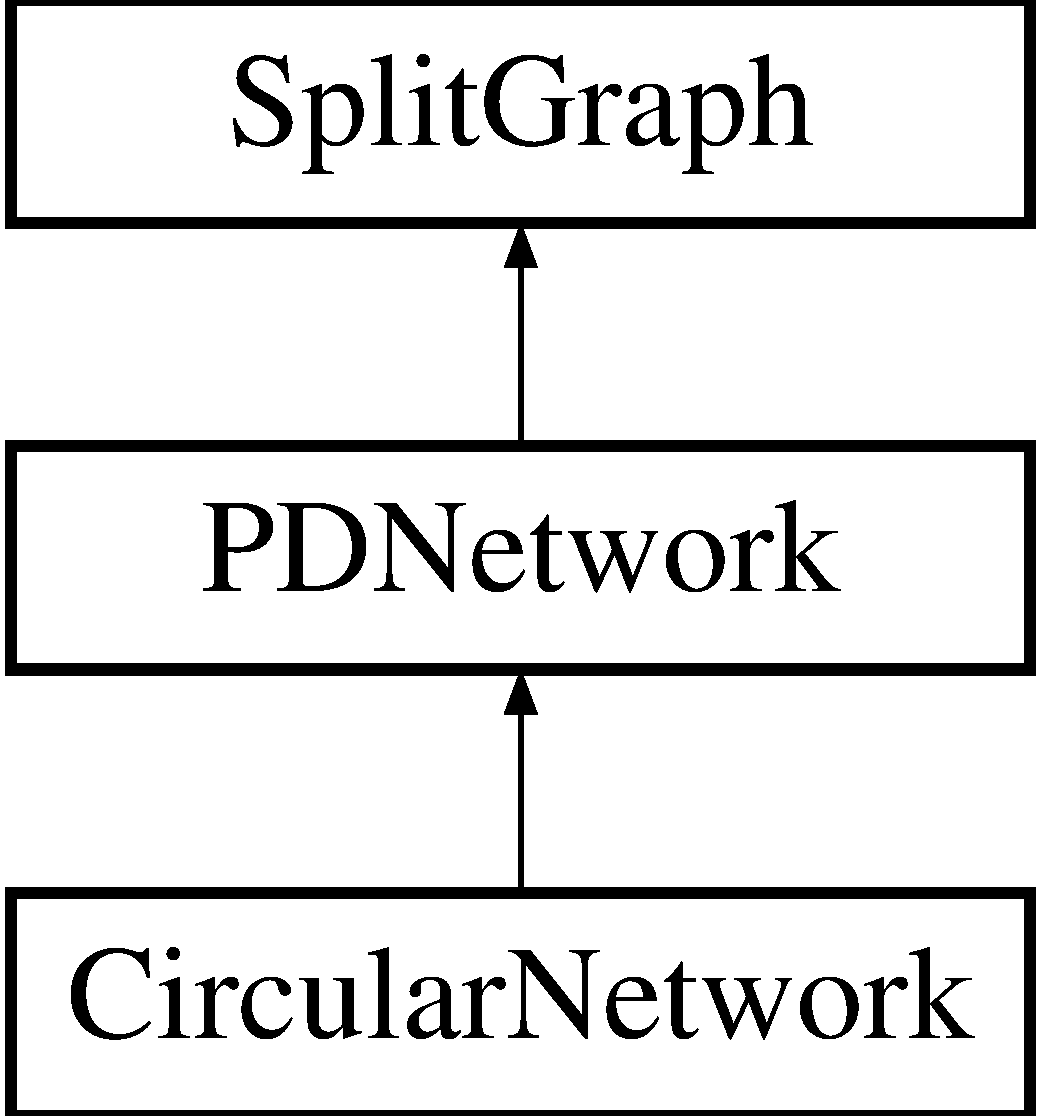
\includegraphics[height=3cm]{classCircularNetwork}
\end{center}
\end{figure}
\subsection*{Public Member Functions}
\begin{DoxyCompactItemize}
\item 
\hyperlink{classCircularNetwork_acc7bc17d879498a780501e2a0bdaec03}{CircularNetwork} ()
\item 
\hyperlink{classCircularNetwork_acdd16c31a1ef6cdcbfeaf60d71e8b47e}{CircularNetwork} (\hyperlink{structParams}{Params} \&params)
\item 
virtual void \hyperlink{classCircularNetwork_a2d7a229ba82a87667c7f194249484f38}{findPD} (\hyperlink{structParams}{Params} \&params, vector$<$ \hyperlink{classSplitSet}{SplitSet} $>$ \&taxa\_\-set, vector$<$ int $>$ \&taxa\_\-order)
\item 
void \hyperlink{classCircularNetwork_a366581f42f10893f5a804073163e609c}{findCircularPD} (\hyperlink{structParams}{Params} \&params, vector$<$ \hyperlink{classSplitSet}{SplitSet} $>$ \&taxa\_\-set, vector$<$ int $>$ \&taxa\_\-order)
\item 
void \hyperlink{classCircularNetwork_af1ee858ebbe97abd3296cad55590f24a}{findCircularRootedPD} (\hyperlink{structParams}{Params} \&params, vector$<$ \hyperlink{classSplitSet}{SplitSet} $>$ \&taxa\_\-set, vector$<$ int $>$ \&taxa\_\-order, int root)
\item 
void \hyperlink{classCircularNetwork_a5fe3bf80c02888d7cacf87a04c041651}{findCircularPDBudget} (\hyperlink{structParams}{Params} \&params, vector$<$ \hyperlink{classSplitSet}{SplitSet} $>$ \&taxa\_\-set, vector$<$ int $>$ \&taxa\_\-order)
\item 
void \hyperlink{classCircularNetwork_ae661db891b7746f63444cb221df89e68}{findCircularRootedPDBudget} (\hyperlink{structParams}{Params} \&params, vector$<$ \hyperlink{classSplitSet}{SplitSet} $>$ \&taxa\_\-set, vector$<$ int $>$ \&taxa\_\-order, int root)
\end{DoxyCompactItemize}
\subsection*{Protected Member Functions}
\begin{DoxyCompactItemize}
\item 
void \hyperlink{classCircularNetwork_acb433def7804457703524e09beea5848}{computePDInfo} (\hyperlink{structParams}{Params} \&params, DoubleMatrix \&table, DoubleMatrix \&dist, int root)
\item 
double \hyperlink{classCircularNetwork_a948222663b8ba7352ef09d037814e25b}{computePDScore} (int sub\_\-size, DoubleMatrix \&table, int root)
\item 
void \hyperlink{classCircularNetwork_a7bfd9c6ef8b4810c421b6613cdd3eecc}{constructPD} (int sub\_\-size, bool find\_\-all, int pd\_\-limit, DoubleMatrix \&table, DoubleMatrix \&dist, \hyperlink{classSplitSet}{SplitSet} \&taxa\_\-set, vector$<$ int $>$ \&taxa\_\-order, int root)
\item 
void \hyperlink{classCircularNetwork_ad4b30f917950be55c1c2b2c5bc66dc3a}{constructPD} (int sub\_\-size, int max\_\-v, int pd\_\-limit, \hyperlink{classSplit}{Split} $\ast$pd\_\-set, DoubleMatrix \&table, DoubleMatrix \&dist, \hyperlink{classSplitSet}{SplitSet} \&taxa\_\-set, vector$<$ int $>$ \&taxa\_\-order, int root)
\item 
void \hyperlink{classCircularNetwork_a71bc1e5b303f8e0b51746e55cd3315e0}{calcMaxBudget} (int budget, matrix(int)\&max\_\-b, vector$<$ int $>$ \&taxa\_\-order)
\item 
void \hyperlink{classCircularNetwork_a18087619b5d6cc0b5c06c8e8daf65709}{constructPDBudget} (int budget, bool find\_\-all, matrix(double)\&table, matrix(double)\&dist, \hyperlink{classSplitSet}{SplitSet} \&taxa\_\-set, vector$<$ int $>$ \&taxa\_\-order, matrix(int)\&max\_\-b, int root)
\item 
void \hyperlink{classCircularNetwork_ac193309edd3ea5117af994273031f344}{constructPDBudget} (int budget, int max\_\-v, \hyperlink{classSplit}{Split} $\ast$pd\_\-set, matrix(double)\&table, matrix(double)\&dist, \hyperlink{classSplitSet}{SplitSet} \&taxa\_\-set, vector$<$ int $>$ \&taxa\_\-order, matrix(int)\&max\_\-b, int root)
\item 
void \hyperlink{classCircularNetwork_a07284c802eadf2367a90ed76eacad4ac}{computePDBudgetInfo} (\hyperlink{structParams}{Params} \&params, matrix(double)\&table, matrix(int)\&id, matrix(double)\&dist, vector$<$ int $>$ \&taxa\_\-order, matrix(int)\&max\_\-b, int root)
\item 
double \hyperlink{classCircularNetwork_a7656f85224812c604e818c4448ac79cf}{computePDBudgetScore} (int budget, matrix(double)\&table, matrix(double)\&dist, vector$<$ int $>$ \&taxa\_\-order, matrix(int)\&max\_\-b, int root)
\end{DoxyCompactItemize}


\subsection{Detailed Description}
Circular Network for PDA algorithm

\begin{DoxyAuthor}{Author}
BUI Quang Minh, Steffen Klaere, Arndt von Haeseler 
\end{DoxyAuthor}


\subsection{Constructor \& Destructor Documentation}
\hypertarget{classCircularNetwork_acc7bc17d879498a780501e2a0bdaec03}{
\index{CircularNetwork@{CircularNetwork}!CircularNetwork@{CircularNetwork}}
\index{CircularNetwork@{CircularNetwork}!CircularNetwork@{CircularNetwork}}
\subsubsection[{CircularNetwork}]{\setlength{\rightskip}{0pt plus 5cm}CircularNetwork::CircularNetwork ()}}
\label{classCircularNetwork_acc7bc17d879498a780501e2a0bdaec03}
empty constructor \hypertarget{classCircularNetwork_acdd16c31a1ef6cdcbfeaf60d71e8b47e}{
\index{CircularNetwork@{CircularNetwork}!CircularNetwork@{CircularNetwork}}
\index{CircularNetwork@{CircularNetwork}!CircularNetwork@{CircularNetwork}}
\subsubsection[{CircularNetwork}]{\setlength{\rightskip}{0pt plus 5cm}CircularNetwork::CircularNetwork ({\bf Params} \& {\em params})}}
\label{classCircularNetwork_acdd16c31a1ef6cdcbfeaf60d71e8b47e}
construct network from a NEXUS file, e.g. produced by SplitsTree 
\begin{DoxyParams}{Parameters}
\item[{\em params}]program parameters \end{DoxyParams}


\subsection{Member Function Documentation}
\hypertarget{classCircularNetwork_a71bc1e5b303f8e0b51746e55cd3315e0}{
\index{CircularNetwork@{CircularNetwork}!calcMaxBudget@{calcMaxBudget}}
\index{calcMaxBudget@{calcMaxBudget}!CircularNetwork@{CircularNetwork}}
\subsubsection[{calcMaxBudget}]{\setlength{\rightskip}{0pt plus 5cm}void CircularNetwork::calcMaxBudget (int {\em budget}, \/  matrix(int)\& {\em max\_\-b}, \/  vector$<$ int $>$ \& {\em taxa\_\-order})\hspace{0.3cm}{\ttfamily  \mbox{[}protected\mbox{]}}}}
\label{classCircularNetwork_a71bc1e5b303f8e0b51746e55cd3315e0}
calculate the maximum budget required from u to v (excluding u and v) 
\begin{DoxyParams}{Parameters}
\item[{\em budget}]total budget \item[{\em max\_\-b}](OUT) max budget matrix between taxa \item[{\em taxa\_\-order}]circular order \end{DoxyParams}
\hypertarget{classCircularNetwork_a07284c802eadf2367a90ed76eacad4ac}{
\index{CircularNetwork@{CircularNetwork}!computePDBudgetInfo@{computePDBudgetInfo}}
\index{computePDBudgetInfo@{computePDBudgetInfo}!CircularNetwork@{CircularNetwork}}
\subsubsection[{computePDBudgetInfo}]{\setlength{\rightskip}{0pt plus 5cm}void CircularNetwork::computePDBudgetInfo ({\bf Params} \& {\em params}, \/  matrix(double)\& {\em table}, \/  matrix(int)\& {\em id}, \/  matrix(double)\& {\em dist}, \/  vector$<$ int $>$ \& {\em taxa\_\-order}, \/  matrix(int)\& {\em max\_\-b}, \/  int {\em root})\hspace{0.3cm}{\ttfamily  \mbox{[}protected\mbox{]}}}}
\label{classCircularNetwork_a07284c802eadf2367a90ed76eacad4ac}
compute the PD information table with budget 
\begin{DoxyParams}{Parameters}
\item[{\em params}]program parameters \item[{\em table}](OUT) computed information \item[{\em id}](OUT) computed information \item[{\em dist}]distance matrix \item[{\em taxa\_\-order}]circular order \item[{\em max\_\-b}]max budget matrix between taxa \item[{\em root}]index of the root taxon \end{DoxyParams}
\hypertarget{classCircularNetwork_a7656f85224812c604e818c4448ac79cf}{
\index{CircularNetwork@{CircularNetwork}!computePDBudgetScore@{computePDBudgetScore}}
\index{computePDBudgetScore@{computePDBudgetScore}!CircularNetwork@{CircularNetwork}}
\subsubsection[{computePDBudgetScore}]{\setlength{\rightskip}{0pt plus 5cm}double CircularNetwork::computePDBudgetScore (int {\em budget}, \/  matrix(double)\& {\em table}, \/  matrix(double)\& {\em dist}, \/  vector$<$ int $>$ \& {\em taxa\_\-order}, \/  matrix(int)\& {\em max\_\-b}, \/  int {\em root})\hspace{0.3cm}{\ttfamily  \mbox{[}protected\mbox{]}}}}
\label{classCircularNetwork_a7656f85224812c604e818c4448ac79cf}
compute the PD score with budget 
\begin{DoxyParams}{Parameters}
\item[{\em budget}]total budget \item[{\em table}](OUT) computed information \item[{\em dist}]distance matrix \item[{\em taxa\_\-order}]circular order \item[{\em max\_\-b}]max budget matrix between taxa \item[{\em root}]index of the root taxon \end{DoxyParams}
\hypertarget{classCircularNetwork_acb433def7804457703524e09beea5848}{
\index{CircularNetwork@{CircularNetwork}!computePDInfo@{computePDInfo}}
\index{computePDInfo@{computePDInfo}!CircularNetwork@{CircularNetwork}}
\subsubsection[{computePDInfo}]{\setlength{\rightskip}{0pt plus 5cm}void CircularNetwork::computePDInfo ({\bf Params} \& {\em params}, \/  DoubleMatrix \& {\em table}, \/  DoubleMatrix \& {\em dist}, \/  int {\em root})\hspace{0.3cm}{\ttfamily  \mbox{[}protected\mbox{]}}}}
\label{classCircularNetwork_acb433def7804457703524e09beea5848}
compute the PD information table 
\begin{DoxyParams}{Parameters}
\item[{\em params}]program parameters \item[{\em table}](OUT) computed information \item[{\em dist}]distance matrix \item[{\em root}]index of the root taxon \end{DoxyParams}
\hypertarget{classCircularNetwork_a948222663b8ba7352ef09d037814e25b}{
\index{CircularNetwork@{CircularNetwork}!computePDScore@{computePDScore}}
\index{computePDScore@{computePDScore}!CircularNetwork@{CircularNetwork}}
\subsubsection[{computePDScore}]{\setlength{\rightskip}{0pt plus 5cm}double CircularNetwork::computePDScore (int {\em sub\_\-size}, \/  DoubleMatrix \& {\em table}, \/  int {\em root})\hspace{0.3cm}{\ttfamily  \mbox{[}protected\mbox{]}}}}
\label{classCircularNetwork_a948222663b8ba7352ef09d037814e25b}
compute the PD score 
\begin{DoxyParams}{Parameters}
\item[{\em sub\_\-size}]the subset size \item[{\em table}]computed information \item[{\em root}]index of the root taxon \end{DoxyParams}
\hypertarget{classCircularNetwork_ad4b30f917950be55c1c2b2c5bc66dc3a}{
\index{CircularNetwork@{CircularNetwork}!constructPD@{constructPD}}
\index{constructPD@{constructPD}!CircularNetwork@{CircularNetwork}}
\subsubsection[{constructPD}]{\setlength{\rightskip}{0pt plus 5cm}void CircularNetwork::constructPD (int {\em sub\_\-size}, \/  int {\em max\_\-v}, \/  int {\em pd\_\-limit}, \/  {\bf Split} $\ast$ {\em pd\_\-set}, \/  DoubleMatrix \& {\em table}, \/  DoubleMatrix \& {\em dist}, \/  {\bf SplitSet} \& {\em taxa\_\-set}, \/  vector$<$ int $>$ \& {\em taxa\_\-order}, \/  int {\em root})\hspace{0.3cm}{\ttfamily  \mbox{[}protected\mbox{]}}}}
\label{classCircularNetwork_ad4b30f917950be55c1c2b2c5bc66dc3a}
construct optimal PD set from computed information for ROOTED case circular network 
\begin{DoxyParams}{Parameters}
\item[{\em sub\_\-size}]the subset size \item[{\em max\_\-v}]end taxon \item[{\em pd\_\-limit}]maximum number of returned PD sets \item[{\em pd\_\-set}]the current constructed PD set \item[{\em table}]computed information \item[{\em dist}]distance matrix \item[{\em taxa\_\-set}](OUT) sets of taxa with optimal PD \item[{\em taxa\_\-order}]circular order \item[{\em root}]the root \end{DoxyParams}
\hypertarget{classCircularNetwork_a7bfd9c6ef8b4810c421b6613cdd3eecc}{
\index{CircularNetwork@{CircularNetwork}!constructPD@{constructPD}}
\index{constructPD@{constructPD}!CircularNetwork@{CircularNetwork}}
\subsubsection[{constructPD}]{\setlength{\rightskip}{0pt plus 5cm}void CircularNetwork::constructPD (int {\em sub\_\-size}, \/  bool {\em find\_\-all}, \/  int {\em pd\_\-limit}, \/  DoubleMatrix \& {\em table}, \/  DoubleMatrix \& {\em dist}, \/  {\bf SplitSet} \& {\em taxa\_\-set}, \/  vector$<$ int $>$ \& {\em taxa\_\-order}, \/  int {\em root})\hspace{0.3cm}{\ttfamily  \mbox{[}protected\mbox{]}}}}
\label{classCircularNetwork_a7bfd9c6ef8b4810c421b6613cdd3eecc}
construct optimal PD set from computed information for ROOTED case circular network 
\begin{DoxyParams}{Parameters}
\item[{\em sub\_\-size}]the subset size \item[{\em find\_\-all}]TRUE of want to find all PD sets \item[{\em pd\_\-limit}]maximum number of returned PD sets \item[{\em table}]computed information \item[{\em dist}]distance matrix \item[{\em taxa\_\-set}](OUT) sets of taxa with optimal PD \item[{\em taxa\_\-order}]circular order \item[{\em root}]the root \end{DoxyParams}
\hypertarget{classCircularNetwork_ac193309edd3ea5117af994273031f344}{
\index{CircularNetwork@{CircularNetwork}!constructPDBudget@{constructPDBudget}}
\index{constructPDBudget@{constructPDBudget}!CircularNetwork@{CircularNetwork}}
\subsubsection[{constructPDBudget}]{\setlength{\rightskip}{0pt plus 5cm}void CircularNetwork::constructPDBudget (int {\em budget}, \/  int {\em max\_\-v}, \/  {\bf Split} $\ast$ {\em pd\_\-set}, \/  matrix(double)\& {\em table}, \/  matrix(double)\& {\em dist}, \/  {\bf SplitSet} \& {\em taxa\_\-set}, \/  vector$<$ int $>$ \& {\em taxa\_\-order}, \/  matrix(int)\& {\em max\_\-b}, \/  int {\em root})\hspace{0.3cm}{\ttfamily  \mbox{[}protected\mbox{]}}}}
\label{classCircularNetwork_ac193309edd3ea5117af994273031f344}
construct optimal PD set from computed information for budget constraint (ROOTED case) 
\begin{DoxyParams}{Parameters}
\item[{\em budget}]total budget \item[{\em max\_\-v}]end taxon \item[{\em pd\_\-set}]the current constructed PD set \item[{\em table}]computed information \item[{\em dist}]distance matrix \item[{\em taxa\_\-set}](OUT) sets of taxa with optimal PD \item[{\em taxa\_\-order}]circular order \item[{\em max\_\-b}]max budget matrix between taxa \item[{\em root}]the root \end{DoxyParams}
\hypertarget{classCircularNetwork_a18087619b5d6cc0b5c06c8e8daf65709}{
\index{CircularNetwork@{CircularNetwork}!constructPDBudget@{constructPDBudget}}
\index{constructPDBudget@{constructPDBudget}!CircularNetwork@{CircularNetwork}}
\subsubsection[{constructPDBudget}]{\setlength{\rightskip}{0pt plus 5cm}void CircularNetwork::constructPDBudget (int {\em budget}, \/  bool {\em find\_\-all}, \/  matrix(double)\& {\em table}, \/  matrix(double)\& {\em dist}, \/  {\bf SplitSet} \& {\em taxa\_\-set}, \/  vector$<$ int $>$ \& {\em taxa\_\-order}, \/  matrix(int)\& {\em max\_\-b}, \/  int {\em root})\hspace{0.3cm}{\ttfamily  \mbox{[}protected\mbox{]}}}}
\label{classCircularNetwork_a18087619b5d6cc0b5c06c8e8daf65709}
construct optimal PD set from computed information for budget constraint (ROOTED case) 
\begin{DoxyParams}{Parameters}
\item[{\em budget}]total budget \item[{\em find\_\-all}]TRUE of want to find all PD sets \item[{\em table}]computed information \item[{\em dist}]distance matrix \item[{\em taxa\_\-set}](OUT) sets of taxa with optimal PD \item[{\em taxa\_\-order}]circular order \item[{\em max\_\-b}]max budget matrix between taxa \item[{\em root}]the root \end{DoxyParams}
\hypertarget{classCircularNetwork_a366581f42f10893f5a804073163e609c}{
\index{CircularNetwork@{CircularNetwork}!findCircularPD@{findCircularPD}}
\index{findCircularPD@{findCircularPD}!CircularNetwork@{CircularNetwork}}
\subsubsection[{findCircularPD}]{\setlength{\rightskip}{0pt plus 5cm}void CircularNetwork::findCircularPD ({\bf Params} \& {\em params}, \/  vector$<$ {\bf SplitSet} $>$ \& {\em taxa\_\-set}, \/  vector$<$ int $>$ \& {\em taxa\_\-order})}}
\label{classCircularNetwork_a366581f42f10893f5a804073163e609c}
dynamic programming algorithm in UNROOTED circular splits graph for phylogenetic diversity of a given size 
\begin{DoxyParams}{Parameters}
\item[{\em params}]parameters \item[{\em taxa\_\-set}](OUT) the set of taxa in the PD-\/set \item[{\em taxa\_\-order}](IN) order of inserted taxa \end{DoxyParams}
\hypertarget{classCircularNetwork_a5fe3bf80c02888d7cacf87a04c041651}{
\index{CircularNetwork@{CircularNetwork}!findCircularPDBudget@{findCircularPDBudget}}
\index{findCircularPDBudget@{findCircularPDBudget}!CircularNetwork@{CircularNetwork}}
\subsubsection[{findCircularPDBudget}]{\setlength{\rightskip}{0pt plus 5cm}void CircularNetwork::findCircularPDBudget ({\bf Params} \& {\em params}, \/  vector$<$ {\bf SplitSet} $>$ \& {\em taxa\_\-set}, \/  vector$<$ int $>$ \& {\em taxa\_\-order})}}
\label{classCircularNetwork_a5fe3bf80c02888d7cacf87a04c041651}
dynamic programming algorithm with cost-\/constrained in UNROOTED circular splits graph for phylogenetic diversity under budget constraint 
\begin{DoxyParams}{Parameters}
\item[{\em params}]program parameters \item[{\em taxa\_\-set}](OUT) the set of taxa in the PD-\/set \item[{\em taxa\_\-order}](IN) order of inserted taxa \end{DoxyParams}
\begin{DoxyReturn}{Returns}
the PD score of the maximal set, also returned in taxa\_\-set.weight 
\end{DoxyReturn}
\hypertarget{classCircularNetwork_af1ee858ebbe97abd3296cad55590f24a}{
\index{CircularNetwork@{CircularNetwork}!findCircularRootedPD@{findCircularRootedPD}}
\index{findCircularRootedPD@{findCircularRootedPD}!CircularNetwork@{CircularNetwork}}
\subsubsection[{findCircularRootedPD}]{\setlength{\rightskip}{0pt plus 5cm}void CircularNetwork::findCircularRootedPD ({\bf Params} \& {\em params}, \/  vector$<$ {\bf SplitSet} $>$ \& {\em taxa\_\-set}, \/  vector$<$ int $>$ \& {\em taxa\_\-order}, \/  int {\em root})}}
\label{classCircularNetwork_af1ee858ebbe97abd3296cad55590f24a}
dynamic programming algorithm in ROOTED circular splits graph for phylogenetic diversity of a given size 
\begin{DoxyParams}{Parameters}
\item[{\em params}]parameters \item[{\em taxa\_\-set}](OUT) the set of taxa in the PD-\/set \item[{\em taxa\_\-order}](IN) order of inserted taxa \item[{\em root}]index of the root taxon \end{DoxyParams}
\hypertarget{classCircularNetwork_ae661db891b7746f63444cb221df89e68}{
\index{CircularNetwork@{CircularNetwork}!findCircularRootedPDBudget@{findCircularRootedPDBudget}}
\index{findCircularRootedPDBudget@{findCircularRootedPDBudget}!CircularNetwork@{CircularNetwork}}
\subsubsection[{findCircularRootedPDBudget}]{\setlength{\rightskip}{0pt plus 5cm}void CircularNetwork::findCircularRootedPDBudget ({\bf Params} \& {\em params}, \/  vector$<$ {\bf SplitSet} $>$ \& {\em taxa\_\-set}, \/  vector$<$ int $>$ \& {\em taxa\_\-order}, \/  int {\em root})}}
\label{classCircularNetwork_ae661db891b7746f63444cb221df89e68}
dynamic programming algorithm with cost-\/constrained in ROOTED circular splits graph for phylogenetic diversity under budget constraint 
\begin{DoxyParams}{Parameters}
\item[{\em params}]program parameters \item[{\em taxa\_\-set}](OUT) the set of taxa in the PD-\/set \item[{\em taxa\_\-order}](IN) order of inserted taxa \end{DoxyParams}
\begin{DoxyReturn}{Returns}
the PD score of the maximal set, also returned in taxa\_\-set.weight 
\end{DoxyReturn}

\begin{DoxyParams}{Parameters}
\item[{\em root}]index of the root taxon \end{DoxyParams}
\hypertarget{classCircularNetwork_a2d7a229ba82a87667c7f194249484f38}{
\index{CircularNetwork@{CircularNetwork}!findPD@{findPD}}
\index{findPD@{findPD}!CircularNetwork@{CircularNetwork}}
\subsubsection[{findPD}]{\setlength{\rightskip}{0pt plus 5cm}void CircularNetwork::findPD ({\bf Params} \& {\em params}, \/  vector$<$ {\bf SplitSet} $>$ \& {\em taxa\_\-set}, \/  vector$<$ int $>$ \& {\em taxa\_\-order})\hspace{0.3cm}{\ttfamily  \mbox{[}virtual\mbox{]}}}}
\label{classCircularNetwork_a2d7a229ba82a87667c7f194249484f38}
MAIN FUNCTION which will call other other findPD depending on the input splits. Search for maximal phylogenetic diversity of a given size 
\begin{DoxyParams}{Parameters}
\item[{\em params}]program parameters \item[{\em taxa\_\-set}](OUT) the set of taxa in the maximal PD set \item[{\em taxa\_\-order}](OUT) order of inserted taxa \end{DoxyParams}


Reimplemented from \hyperlink{classPDNetwork_ae481d52c7f411e1fa1f768746329130b}{PDNetwork}.

The documentation for this class was generated from the following files:\begin{DoxyCompactItemize}
\item 
src/circularnetwork.h\item 
src/circularnetwork.cpp\end{DoxyCompactItemize}

\hypertarget{classEigenDecomposition}{
\section{EigenDecomposition Class Reference}
\label{classEigenDecomposition}\index{EigenDecomposition@{EigenDecomposition}}
}


{\ttfamily \#include $<$eigendecomposition.h$>$}Inheritance diagram for EigenDecomposition::\begin{figure}[H]
\begin{center}
\leavevmode
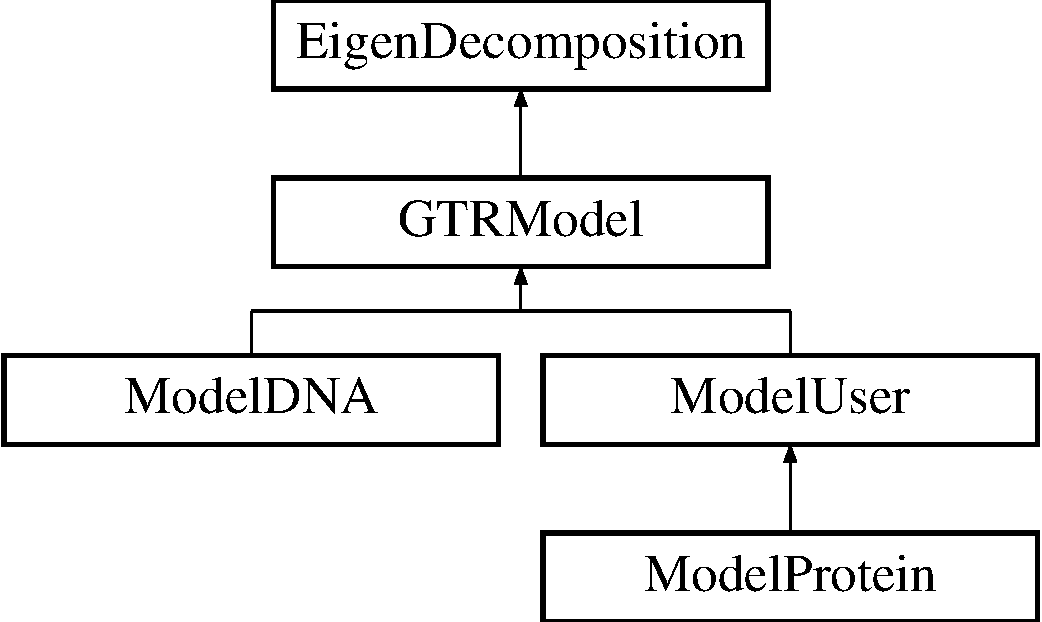
\includegraphics[height=4cm]{classEigenDecomposition}
\end{center}
\end{figure}
\subsection*{Public Member Functions}
\begin{DoxyCompactItemize}
\item 
void \hyperlink{classEigenDecomposition_a9d97980b08c8f486b7ef26afff08947f}{eigensystem\_\-sym} (double $\ast$$\ast$rate\_\-params, double $\ast$state\_\-freq, double $\ast$eval, double $\ast$$\ast$evec, double $\ast$$\ast$inv\_\-evec, int num\_\-state)
\end{DoxyCompactItemize}
\subsection*{Protected Attributes}
\begin{DoxyCompactItemize}
\item 
double \hyperlink{classEigenDecomposition_ad628b6f3a05b9ba605698b9814f81e6f}{total\_\-num\_\-subst}
\end{DoxyCompactItemize}


\subsection{Detailed Description}
Eigenvalues, eigenvectors decomposition

\begin{DoxyAuthor}{Author}
BUI Quang Minh $<$\href{mailto:minh.bui@univie.ac.at}{\tt minh.bui@univie.ac.at}$>$ 
\end{DoxyAuthor}


\subsection{Member Function Documentation}
\hypertarget{classEigenDecomposition_a9d97980b08c8f486b7ef26afff08947f}{
\index{EigenDecomposition@{EigenDecomposition}!eigensystem\_\-sym@{eigensystem\_\-sym}}
\index{eigensystem\_\-sym@{eigensystem\_\-sym}!EigenDecomposition@{EigenDecomposition}}
\subsubsection[{eigensystem\_\-sym}]{\setlength{\rightskip}{0pt plus 5cm}void EigenDecomposition::eigensystem\_\-sym (double $\ast$$\ast$ {\em rate\_\-params}, \/  double $\ast$ {\em state\_\-freq}, \/  double $\ast$ {\em eval}, \/  double $\ast$$\ast$ {\em evec}, \/  double $\ast$$\ast$ {\em inv\_\-evec}, \/  int {\em num\_\-state})}}
\label{classEigenDecomposition_a9d97980b08c8f486b7ef26afff08947f}
EigenSystem for symmetric matrix 
\begin{DoxyParams}{Parameters}
\item[{\em rate\_\-params}]rate parameters (not the rate matrix) \item[{\em state\_\-freq}]state frequencies \item[{\em eval}](OUT) eigenvalues \item[{\em evec}](OUT) eigenvectors \item[{\em inv\_\-evec}](OUT) inverse matrix of eigenvectors \item[{\em num\_\-state}](IN) number of states \end{DoxyParams}


\subsection{Member Data Documentation}
\hypertarget{classEigenDecomposition_ad628b6f3a05b9ba605698b9814f81e6f}{
\index{EigenDecomposition@{EigenDecomposition}!total\_\-num\_\-subst@{total\_\-num\_\-subst}}
\index{total\_\-num\_\-subst@{total\_\-num\_\-subst}!EigenDecomposition@{EigenDecomposition}}
\subsubsection[{total\_\-num\_\-subst}]{\setlength{\rightskip}{0pt plus 5cm}double {\bf EigenDecomposition::total\_\-num\_\-subst}\hspace{0.3cm}{\ttfamily  \mbox{[}protected\mbox{]}}}}
\label{classEigenDecomposition_ad628b6f3a05b9ba605698b9814f81e6f}
the total number of substitutions per unit time 

The documentation for this class was generated from the following files:\begin{DoxyCompactItemize}
\item 
src/eigendecomposition.h\item 
src/eigendecomposition.cpp\end{DoxyCompactItemize}

\hypertarget{structstd_1_1equal__to_3_01Split_01_5_01_4}{
\section{std::equal\_\-to$<$ Split $\ast$ $>$ Struct Template Reference}
\label{structstd_1_1equal__to_3_01Split_01_5_01_4}\index{std::equal\_\-to$<$ Split $\ast$ $>$@{std::equal\_\-to$<$ Split $\ast$ $>$}}
}


{\ttfamily \#include $<$hashsplitset.h$>$}\subsection*{Public Member Functions}
\begin{DoxyCompactItemize}
\item 
bool \hyperlink{structstd_1_1equal__to_3_01Split_01_5_01_4_aea844965cab3be25f669b684bef7dc21}{operator()} (const \hyperlink{classSplit}{Split} $\ast$s1, const \hyperlink{classSplit}{Split} $\ast$s2) const 
\end{DoxyCompactItemize}


\subsection{Detailed Description}
\subsubsection*{template$<$$>$ struct std::equal\_\-to$<$ Split $\ast$ $>$}

Define equal\_\-to of two splits, used for hash\_\-set (or hash\_\-map) template 

\subsection{Member Function Documentation}
\hypertarget{structstd_1_1equal__to_3_01Split_01_5_01_4_aea844965cab3be25f669b684bef7dc21}{
\index{std::equal\_\-to$<$ Split $\ast$ $>$@{std::equal\_\-to$<$ Split $\ast$ $>$}!operator()@{operator()}}
\index{operator()@{operator()}!std::equal_to< Split * >@{std::equal\_\-to$<$ Split $\ast$ $>$}}
\subsubsection[{operator()}]{\setlength{\rightskip}{0pt plus 5cm}bool std::equal\_\-to$<$ {\bf Split} $\ast$ $>$::operator() (const {\bf Split} $\ast$ {\em s1}, \/  const {\bf Split} $\ast$ {\em s2}) const\hspace{0.3cm}{\ttfamily  \mbox{[}inline\mbox{]}}}}
\label{structstd_1_1equal__to_3_01Split_01_5_01_4_aea844965cab3be25f669b684bef7dc21}
\begin{DoxyReturn}{Returns}
true if $\ast$s1 == $\ast$s2 
\end{DoxyReturn}

\begin{DoxyParams}{Parameters}
\item[{\em s1}]first split \item[{\em s2}]second split \end{DoxyParams}


The documentation for this struct was generated from the following file:\begin{DoxyCompactItemize}
\item 
src/hashsplitset.h\end{DoxyCompactItemize}

\hypertarget{classGreedy}{
\section{Greedy Class Reference}
\label{classGreedy}\index{Greedy@{Greedy}}
}


{\ttfamily \#include $<$greedy.h$>$}Inheritance diagram for Greedy::\begin{figure}[H]
\begin{center}
\leavevmode
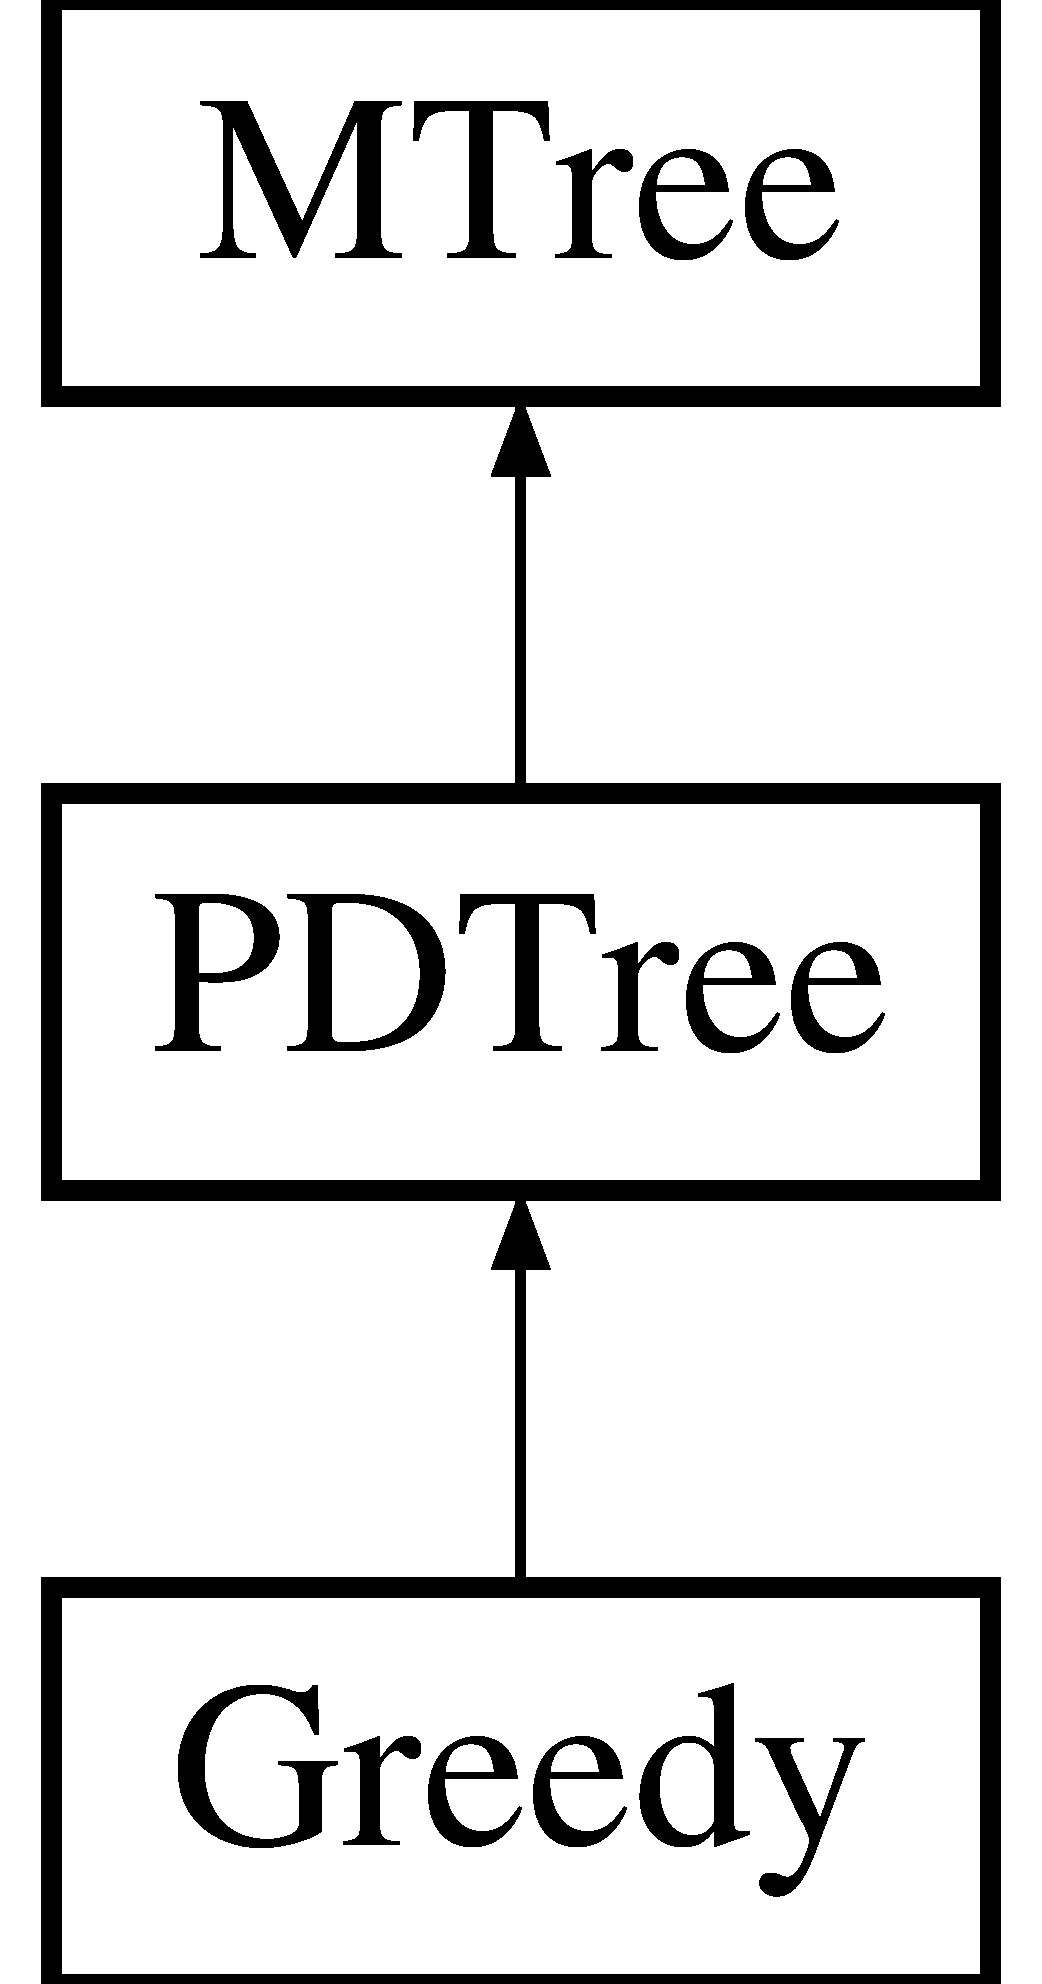
\includegraphics[height=3cm]{classGreedy}
\end{center}
\end{figure}
\subsection*{Public Member Functions}
\begin{DoxyCompactItemize}
\item 
\hyperlink{classGreedy_a1aeec7fbb70ebb2abe0fcb97f21995d8}{Greedy} (\hyperlink{structParams}{Params} \&params)
\item 
\hyperlink{classGreedy_ab5f9558f6a84338ab866c11bffa934cc}{Greedy} (\hyperlink{classPDTree}{PDTree} \&tree)
\item 
\hyperlink{classGreedy_a916c0ab051f780c4d3ccec06f44bbf6c}{Greedy} ()
\item 
void \hyperlink{classGreedy_a9e5abfe8869f9e6695f77748d6fe5e51}{run} (\hyperlink{structParams}{Params} \&params, vector$<$ \hyperlink{classPDTaxaSet}{PDTaxaSet} $>$ \&taxa\_\-set)
\item 
void \hyperlink{classGreedy_a933a3b9c40efec6d2643092baccf6b7f}{updateOnLongestPath} (\hyperlink{classNode}{Node} $\ast$node, NodeVector \&\hyperlink{classGreedy_ac7f2cff520d775503d290e236fce8baf}{subtree}, \hyperlink{classPDTaxaSet}{PDTaxaSet} \&cur\_\-set)
\item 
void \hyperlink{classGreedy_a52d592f837f77cd51b39b8f4c3f64e0c}{buildOnInitialSet} (NodeVector \&\hyperlink{classGreedy_ac7f2cff520d775503d290e236fce8baf}{subtree}, NodeVector \&nodestack, \hyperlink{classNode}{Node} $\ast$node=NULL, \hyperlink{classNode}{Node} $\ast$dad=NULL)
\item 
double \hyperlink{classGreedy_a0f31932ace48884fa0b6aadbd444229d}{updateOnInitialSet} (NodeVector \&\hyperlink{classGreedy_ac7f2cff520d775503d290e236fce8baf}{subtree})
\item 
NeighborSet::iterator \hyperlink{classGreedy_a6b90a3f292fcf91be8f0a156e67822f0}{highestNeighbor} ()
\item 
void \hyperlink{classGreedy_aaa333c0d2919689abfe5a439f4e41b6a}{addNeighbor} (\hyperlink{classNeighbor}{Neighbor} $\ast$neigh)
\end{DoxyCompactItemize}
\subsection*{Public Attributes}
\begin{DoxyCompactItemize}
\item 
NeighborSet \hyperlink{classGreedy_a56a5f478b16b0da1304d79d03d390ab0}{neighset}
\item 
NodeVector \hyperlink{classGreedy_ac7f2cff520d775503d290e236fce8baf}{subtree}
\end{DoxyCompactItemize}


\subsection{Detailed Description}
Implementation of greedy algorithm with complexity O(n$\ast$logk) \begin{DoxyAuthor}{Author}
BUI Quang Minh, Steffen Klaere, Arndt von Haeseler 
\end{DoxyAuthor}


\subsection{Constructor \& Destructor Documentation}
\hypertarget{classGreedy_a1aeec7fbb70ebb2abe0fcb97f21995d8}{
\index{Greedy@{Greedy}!Greedy@{Greedy}}
\index{Greedy@{Greedy}!Greedy@{Greedy}}
\subsubsection[{Greedy}]{\setlength{\rightskip}{0pt plus 5cm}Greedy::Greedy ({\bf Params} \& {\em params})\hspace{0.3cm}{\ttfamily  \mbox{[}inline\mbox{]}}}}
\label{classGreedy_a1aeec7fbb70ebb2abe0fcb97f21995d8}
construct from program parameters 
\begin{DoxyParams}{Parameters}
\item[{\em params}]program parameters \end{DoxyParams}
\hypertarget{classGreedy_ab5f9558f6a84338ab866c11bffa934cc}{
\index{Greedy@{Greedy}!Greedy@{Greedy}}
\index{Greedy@{Greedy}!Greedy@{Greedy}}
\subsubsection[{Greedy}]{\setlength{\rightskip}{0pt plus 5cm}Greedy::Greedy ({\bf PDTree} \& {\em tree})\hspace{0.3cm}{\ttfamily  \mbox{[}inline\mbox{]}}}}
\label{classGreedy_ab5f9558f6a84338ab866c11bffa934cc}
construct from a tree 
\begin{DoxyParams}{Parameters}
\item[{\em tree}]a tree class \end{DoxyParams}
\hypertarget{classGreedy_a916c0ab051f780c4d3ccec06f44bbf6c}{
\index{Greedy@{Greedy}!Greedy@{Greedy}}
\index{Greedy@{Greedy}!Greedy@{Greedy}}
\subsubsection[{Greedy}]{\setlength{\rightskip}{0pt plus 5cm}Greedy::Greedy ()\hspace{0.3cm}{\ttfamily  \mbox{[}inline\mbox{]}}}}
\label{classGreedy_a916c0ab051f780c4d3ccec06f44bbf6c}
constructor 

\subsection{Member Function Documentation}
\hypertarget{classGreedy_aaa333c0d2919689abfe5a439f4e41b6a}{
\index{Greedy@{Greedy}!addNeighbor@{addNeighbor}}
\index{addNeighbor@{addNeighbor}!Greedy@{Greedy}}
\subsubsection[{addNeighbor}]{\setlength{\rightskip}{0pt plus 5cm}void Greedy::addNeighbor ({\bf Neighbor} $\ast$ {\em neigh})}}
\label{classGreedy_aaa333c0d2919689abfe5a439f4e41b6a}
add an edge into the NeighborSet \hypertarget{classGreedy_a52d592f837f77cd51b39b8f4c3f64e0c}{
\index{Greedy@{Greedy}!buildOnInitialSet@{buildOnInitialSet}}
\index{buildOnInitialSet@{buildOnInitialSet}!Greedy@{Greedy}}
\subsubsection[{buildOnInitialSet}]{\setlength{\rightskip}{0pt plus 5cm}void Greedy::buildOnInitialSet (NodeVector \& {\em subtree}, \/  NodeVector \& {\em nodestack}, \/  {\bf Node} $\ast$ {\em node} = {\ttfamily NULL}, \/  {\bf Node} $\ast$ {\em dad} = {\ttfamily NULL})}}
\label{classGreedy_a52d592f837f77cd51b39b8f4c3f64e0c}
build the initial subtree based on the initial set of taxa 
\begin{DoxyParams}{Parameters}
\item[{\em node}]the starting node, NULL to start from the root \item[{\em dad}]dad of the node, used to direct the search \item[{\em subtree}](OUT) resulted subtree \item[{\em nodestack}](TEMP) stack of node, used only by function\end{DoxyParams}
initialize the ordered list based on the initial tree structure \hypertarget{classGreedy_a6b90a3f292fcf91be8f0a156e67822f0}{
\index{Greedy@{Greedy}!highestNeighbor@{highestNeighbor}}
\index{highestNeighbor@{highestNeighbor}!Greedy@{Greedy}}
\subsubsection[{highestNeighbor}]{\setlength{\rightskip}{0pt plus 5cm}NeighborSet::iterator Greedy::highestNeighbor ()}}
\label{classGreedy_a6b90a3f292fcf91be8f0a156e67822f0}
\begin{DoxyReturn}{Returns}
innodes.begin(). 
\end{DoxyReturn}
\hypertarget{classGreedy_a9e5abfe8869f9e6695f77748d6fe5e51}{
\index{Greedy@{Greedy}!run@{run}}
\index{run@{run}!Greedy@{Greedy}}
\subsubsection[{run}]{\setlength{\rightskip}{0pt plus 5cm}void Greedy::run ({\bf Params} \& {\em params}, \/  vector$<$ {\bf PDTaxaSet} $>$ \& {\em taxa\_\-set})}}
\label{classGreedy_a9e5abfe8869f9e6695f77748d6fe5e51}
run the algorithm 
\begin{DoxyParams}{Parameters}
\item[{\em params}]program parameters \item[{\em taxa\_\-set}](OUT) vector of PD sets\end{DoxyParams}
run the algorithm \hypertarget{classGreedy_a0f31932ace48884fa0b6aadbd444229d}{
\index{Greedy@{Greedy}!updateOnInitialSet@{updateOnInitialSet}}
\index{updateOnInitialSet@{updateOnInitialSet}!Greedy@{Greedy}}
\subsubsection[{updateOnInitialSet}]{\setlength{\rightskip}{0pt plus 5cm}double Greedy::updateOnInitialSet (NodeVector \& {\em subtree})}}
\label{classGreedy_a0f31932ace48884fa0b6aadbd444229d}
initialize the ordered list based on the initial subtree structure 
\begin{DoxyParams}{Parameters}
\item[{\em subtree}]vector containing nodes in the subtree \end{DoxyParams}
\begin{DoxyReturn}{Returns}
the subtree length 
\end{DoxyReturn}
\hypertarget{classGreedy_a933a3b9c40efec6d2643092baccf6b7f}{
\index{Greedy@{Greedy}!updateOnLongestPath@{updateOnLongestPath}}
\index{updateOnLongestPath@{updateOnLongestPath}!Greedy@{Greedy}}
\subsubsection[{updateOnLongestPath}]{\setlength{\rightskip}{0pt plus 5cm}void Greedy::updateOnLongestPath ({\bf Node} $\ast$ {\em node}, \/  NodeVector \& {\em subtree}, \/  {\bf PDTaxaSet} \& {\em cur\_\-set})}}
\label{classGreedy_a933a3b9c40efec6d2643092baccf6b7f}
update the ordered list based on the recent longest path 
\begin{DoxyParams}{Parameters}
\item[{\em node}]the starting node \item[{\em subtree}](OUT) resulted subtree \item[{\em cur\_\-set}]the current set \end{DoxyParams}


\subsection{Member Data Documentation}
\hypertarget{classGreedy_a56a5f478b16b0da1304d79d03d390ab0}{
\index{Greedy@{Greedy}!neighset@{neighset}}
\index{neighset@{neighset}!Greedy@{Greedy}}
\subsubsection[{neighset}]{\setlength{\rightskip}{0pt plus 5cm}NeighborSet {\bf Greedy::neighset}}}
\label{classGreedy_a56a5f478b16b0da1304d79d03d390ab0}
neighbor set \hypertarget{classGreedy_ac7f2cff520d775503d290e236fce8baf}{
\index{Greedy@{Greedy}!subtree@{subtree}}
\index{subtree@{subtree}!Greedy@{Greedy}}
\subsubsection[{subtree}]{\setlength{\rightskip}{0pt plus 5cm}NodeVector {\bf Greedy::subtree}}}
\label{classGreedy_ac7f2cff520d775503d290e236fce8baf}
list of nodes in the subtree 

The documentation for this class was generated from the following files:\begin{DoxyCompactItemize}
\item 
src/greedy.h\item 
src/greedy.cpp\end{DoxyCompactItemize}

\hypertarget{classGTRModel}{
\section{GTRModel Class Reference}
\label{classGTRModel}\index{GTRModel@{GTRModel}}
}


{\ttfamily \#include $<$gtrmodel.h$>$}Inheritance diagram for GTRModel::\begin{figure}[H]
\begin{center}
\leavevmode
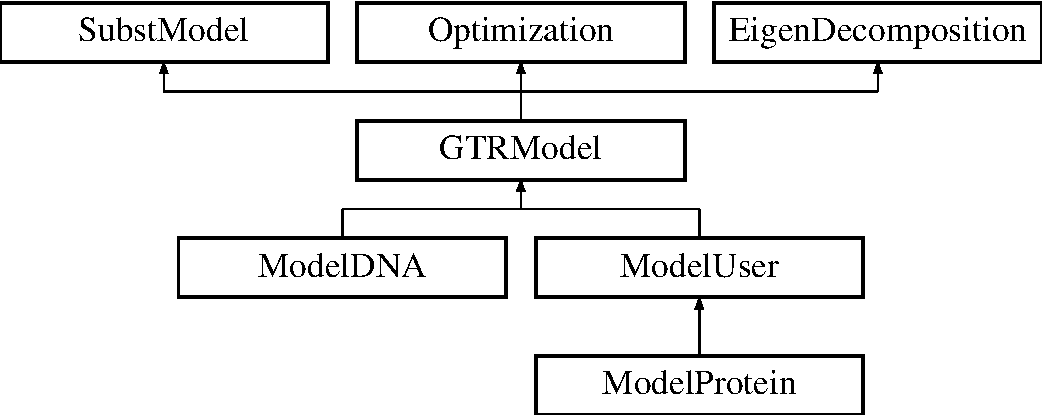
\includegraphics[height=4cm]{classGTRModel}
\end{center}
\end{figure}
\subsection*{Public Member Functions}
\begin{DoxyCompactItemize}
\item 
\hyperlink{classGTRModel_a6c79a459f383e64ee9540eaf8b854827}{GTRModel} (\hyperlink{classPhyloTree}{PhyloTree} $\ast$tree)
\item 
void \hyperlink{classGTRModel_a6a5736bfb839fca17dc6db2ee1cf91d5}{init} (StateFreqType \hyperlink{classGTRModel_a699318690979ff66c655dd3022d5127a}{freq\_\-type})
\item 
virtual void \hyperlink{classGTRModel_ad0625a75ce5e8f5fca7f65657b2677b8}{init} (const char $\ast$model\_\-name, StateFreqType \hyperlink{classGTRModel_a699318690979ff66c655dd3022d5127a}{freq\_\-type})
\item 
virtual \hyperlink{classGTRModel_aca20597dad26270745e2e82c771b5ee9}{$\sim$GTRModel} ()
\item 
void \hyperlink{classGTRModel_a121f6e38dae476820555a66ed3e6f10a}{setTree} (\hyperlink{classPhyloTree}{PhyloTree} $\ast$tree)
\item 
virtual void \hyperlink{classGTRModel_aa779b66b3824c4e956db7b56dee668c2}{computeTransMatrix} (double time, double $\ast$trans\_\-matrix)
\item 
virtual void \hyperlink{classGTRModel_aa7cdd1fb6852faccc185284c075c918b}{getStateFrequency} (double $\ast$\hyperlink{classGTRModel_a03c2ca5094d8c6563dbded5a05b26319}{state\_\-freq})
\item 
virtual void \hyperlink{classGTRModel_a9f6c7532d57b0e41d95dd95c5972cf5b}{computeTransDerv} (double time, double $\ast$trans\_\-matrix, double $\ast$trans\_\-derv1, double $\ast$trans\_\-derv2)
\item 
StateFreqType \hyperlink{classGTRModel_af2447a8e79a031706028d36beb6931bd}{getFreqType} ()
\item 
virtual int \hyperlink{classGTRModel_a6e2066898fbbb245596d4a97dd8ee33c}{getNDim} ()
\item 
virtual double \hyperlink{classGTRModel_ac32444cf94b5c3f3240aa344d4bc40b1}{targetFunk} (double x\mbox{[}$\,$\mbox{]})
\item 
virtual double \hyperlink{classGTRModel_a01c47ec7ac4b856e60aa3e4339e0044a}{optimizeParameters} ()
\item 
virtual void \hyperlink{classGTRModel_a233f9b473e4e3c549d801ff8a084e35e}{writeInfo} (ostream \&out)
\item 
virtual void \hyperlink{classGTRModel_a3dd6bc6cb405e76346eac7b813687a20}{writeParameters} (ostream \&out)
\item 
void \hyperlink{classGTRModel_ab73647f93c4fdde88c62a775586ae9ea}{decomposeRateMatrix} ()
\end{DoxyCompactItemize}
\subsection*{Protected Member Functions}
\begin{DoxyCompactItemize}
\item 
virtual void \hyperlink{classGTRModel_a1231f10a523ef280e1862b18b0549aa6}{setVariables} (double $\ast$variables)
\item 
virtual void \hyperlink{classGTRModel_ae0d291e293dd142d41466650539a2481}{getVariables} (double $\ast$variables)
\end{DoxyCompactItemize}
\subsection*{Protected Attributes}
\begin{DoxyCompactItemize}
\item 
\hyperlink{classPhyloTree}{PhyloTree} $\ast$ \hyperlink{classGTRModel_a21785f014f182f075d608cfc9118e6fb}{phylo\_\-tree}
\item 
double $\ast$ \hyperlink{classGTRModel_ad194dff1b132c09e4c2ebff0f8cdedab}{rates}
\item 
double $\ast$ \hyperlink{classGTRModel_a03c2ca5094d8c6563dbded5a05b26319}{state\_\-freq}
\item 
StateFreqType \hyperlink{classGTRModel_a699318690979ff66c655dd3022d5127a}{freq\_\-type}
\item 
double $\ast$ \hyperlink{classGTRModel_a162f4d6889a320c2753ea31d6c0b03f1}{eigenvalues}
\item 
double $\ast$$\ast$ \hyperlink{classGTRModel_ab8e201929a6d84d9bd2e58d0a3e03b5b}{eigenvectors}
\item 
double $\ast$$\ast$ \hyperlink{classGTRModel_a74c9c92fe909714d09f75fdcb8459ac9}{inv\_\-eigenvectors}
\item 
double $\ast$ \hyperlink{classGTRModel_a79645d7740f239a3a101c0b58fcb236c}{eigen\_\-coeff}
\end{DoxyCompactItemize}


\subsection{Detailed Description}
General Time Reversible (GTR) model of substitution. This works for all kind of data, not only DNA

\begin{DoxyAuthor}{Author}
BUI Quang Minh $<$\href{mailto:minh.bui@univie.ac.at}{\tt minh.bui@univie.ac.at}$>$ 
\end{DoxyAuthor}


\subsection{Constructor \& Destructor Documentation}
\hypertarget{classGTRModel_a6c79a459f383e64ee9540eaf8b854827}{
\index{GTRModel@{GTRModel}!GTRModel@{GTRModel}}
\index{GTRModel@{GTRModel}!GTRModel@{GTRModel}}
\subsubsection[{GTRModel}]{\setlength{\rightskip}{0pt plus 5cm}GTRModel::GTRModel ({\bf PhyloTree} $\ast$ {\em tree})}}
\label{classGTRModel_a6c79a459f383e64ee9540eaf8b854827}
constructor 
\begin{DoxyParams}{Parameters}
\item[{\em tree}]associated tree for the model \end{DoxyParams}
\hypertarget{classGTRModel_aca20597dad26270745e2e82c771b5ee9}{
\index{GTRModel@{GTRModel}!$\sim$GTRModel@{$\sim$GTRModel}}
\index{$\sim$GTRModel@{$\sim$GTRModel}!GTRModel@{GTRModel}}
\subsubsection[{$\sim$GTRModel}]{\setlength{\rightskip}{0pt plus 5cm}GTRModel::$\sim$GTRModel ()\hspace{0.3cm}{\ttfamily  \mbox{[}virtual\mbox{]}}}}
\label{classGTRModel_aca20597dad26270745e2e82c771b5ee9}
destructor 

\subsection{Member Function Documentation}
\hypertarget{classGTRModel_a9f6c7532d57b0e41d95dd95c5972cf5b}{
\index{GTRModel@{GTRModel}!computeTransDerv@{computeTransDerv}}
\index{computeTransDerv@{computeTransDerv}!GTRModel@{GTRModel}}
\subsubsection[{computeTransDerv}]{\setlength{\rightskip}{0pt plus 5cm}void GTRModel::computeTransDerv (double {\em time}, \/  double $\ast$ {\em trans\_\-matrix}, \/  double $\ast$ {\em trans\_\-derv1}, \/  double $\ast$ {\em trans\_\-derv2})\hspace{0.3cm}{\ttfamily  \mbox{[}virtual\mbox{]}}}}
\label{classGTRModel_a9f6c7532d57b0e41d95dd95c5972cf5b}
compute the transition probability matrix.and the derivative 1 and 2 
\begin{DoxyParams}{Parameters}
\item[{\em time}]time between two events \item[{\em trans\_\-matrix}](OUT) the transition matrix between all pairs of states. Assume trans\_\-matrix has size of num\_\-states $\ast$ num\_\-states. \item[{\em trans\_\-derv1}](OUT) the 1st derivative matrix between all pairs of states. \item[{\em trans\_\-derv2}](OUT) the 2nd derivative matrix between all pairs of states. \end{DoxyParams}


Reimplemented from \hyperlink{classSubstModel_ada88db5c6befc33de5ddb590667ba865}{SubstModel}.\hypertarget{classGTRModel_aa779b66b3824c4e956db7b56dee668c2}{
\index{GTRModel@{GTRModel}!computeTransMatrix@{computeTransMatrix}}
\index{computeTransMatrix@{computeTransMatrix}!GTRModel@{GTRModel}}
\subsubsection[{computeTransMatrix}]{\setlength{\rightskip}{0pt plus 5cm}void GTRModel::computeTransMatrix (double {\em time}, \/  double $\ast$ {\em trans\_\-matrix})\hspace{0.3cm}{\ttfamily  \mbox{[}virtual\mbox{]}}}}
\label{classGTRModel_aa779b66b3824c4e956db7b56dee668c2}
compute the transition probability matrix. 
\begin{DoxyParams}{Parameters}
\item[{\em time}]time between two events \item[{\em trans\_\-matrix}](OUT) the transition matrix between all pairs of states. Assume trans\_\-matrix has size of num\_\-states $\ast$ num\_\-states. \end{DoxyParams}


Reimplemented from \hyperlink{classSubstModel_a83997a2aaea95f2c994d88a9d1cb190e}{SubstModel}.\hypertarget{classGTRModel_ab73647f93c4fdde88c62a775586ae9ea}{
\index{GTRModel@{GTRModel}!decomposeRateMatrix@{decomposeRateMatrix}}
\index{decomposeRateMatrix@{decomposeRateMatrix}!GTRModel@{GTRModel}}
\subsubsection[{decomposeRateMatrix}]{\setlength{\rightskip}{0pt plus 5cm}void GTRModel::decomposeRateMatrix ()}}
\label{classGTRModel_ab73647f93c4fdde88c62a775586ae9ea}
decompose the rate matrix into eigenvalues and eigenvectors \hypertarget{classGTRModel_af2447a8e79a031706028d36beb6931bd}{
\index{GTRModel@{GTRModel}!getFreqType@{getFreqType}}
\index{getFreqType@{getFreqType}!GTRModel@{GTRModel}}
\subsubsection[{getFreqType}]{\setlength{\rightskip}{0pt plus 5cm}StateFreqType GTRModel::getFreqType ()\hspace{0.3cm}{\ttfamily  \mbox{[}inline\mbox{]}}}}
\label{classGTRModel_af2447a8e79a031706028d36beb6931bd}
get frequency type \begin{DoxyReturn}{Returns}
frequency type 
\end{DoxyReturn}
\hypertarget{classGTRModel_a6e2066898fbbb245596d4a97dd8ee33c}{
\index{GTRModel@{GTRModel}!getNDim@{getNDim}}
\index{getNDim@{getNDim}!GTRModel@{GTRModel}}
\subsubsection[{getNDim}]{\setlength{\rightskip}{0pt plus 5cm}int GTRModel::getNDim ()\hspace{0.3cm}{\ttfamily  \mbox{[}virtual\mbox{]}}}}
\label{classGTRModel_a6e2066898fbbb245596d4a97dd8ee33c}
\begin{DoxyReturn}{Returns}
the number of dimensions 
\end{DoxyReturn}


Reimplemented from \hyperlink{classOptimization_a6d04cefb0969f3cac9b607aa1412eb57}{Optimization}.

Reimplemented in \hyperlink{classModelDNA_adc73fda51fb0f02049ed891b29c3a951}{ModelDNA}, and \hyperlink{classModelUser_ad5a88a6c25475b8bb0ea778f4c40cf3b}{ModelUser}.\hypertarget{classGTRModel_aa7cdd1fb6852faccc185284c075c918b}{
\index{GTRModel@{GTRModel}!getStateFrequency@{getStateFrequency}}
\index{getStateFrequency@{getStateFrequency}!GTRModel@{GTRModel}}
\subsubsection[{getStateFrequency}]{\setlength{\rightskip}{0pt plus 5cm}void GTRModel::getStateFrequency (double $\ast$ {\em state\_\-freq})\hspace{0.3cm}{\ttfamily  \mbox{[}virtual\mbox{]}}}}
\label{classGTRModel_aa7cdd1fb6852faccc185284c075c918b}
compute the state frequency vector 
\begin{DoxyParams}{Parameters}
\item[{\em state\_\-freq}](OUT) state frequency vector. Assume state\_\-freq has size of num\_\-states \end{DoxyParams}


Reimplemented from \hyperlink{classSubstModel_a18f98e25cacbd18e1b64b25d10a3e11f}{SubstModel}.\hypertarget{classGTRModel_ae0d291e293dd142d41466650539a2481}{
\index{GTRModel@{GTRModel}!getVariables@{getVariables}}
\index{getVariables@{getVariables}!GTRModel@{GTRModel}}
\subsubsection[{getVariables}]{\setlength{\rightskip}{0pt plus 5cm}void GTRModel::getVariables (double $\ast$ {\em variables})\hspace{0.3cm}{\ttfamily  \mbox{[}protected, virtual\mbox{]}}}}
\label{classGTRModel_ae0d291e293dd142d41466650539a2481}
this function is served for the multi-\/dimension optimization. It should assign the model parameters from a vector of variables that is index from 1 (NOTE: not from 0) 
\begin{DoxyParams}{Parameters}
\item[{\em variables}]vector of variables, indexed from 1 \end{DoxyParams}


Reimplemented in \hyperlink{classModelDNA_a4083dfee9b55936019483c5e9a4bb2f7}{ModelDNA}.\hypertarget{classGTRModel_ad0625a75ce5e8f5fca7f65657b2677b8}{
\index{GTRModel@{GTRModel}!init@{init}}
\index{init@{init}!GTRModel@{GTRModel}}
\subsubsection[{init}]{\setlength{\rightskip}{0pt plus 5cm}virtual void GTRModel::init (const char $\ast$ {\em model\_\-name}, \/  StateFreqType {\em freq\_\-type})\hspace{0.3cm}{\ttfamily  \mbox{[}inline, virtual\mbox{]}}}}
\label{classGTRModel_ad0625a75ce5e8f5fca7f65657b2677b8}
this function is served for \hyperlink{classModelDNA}{ModelDNA} and \hyperlink{classModelProtein}{ModelProtein} 
\begin{DoxyParams}{Parameters}
\item[{\em model\_\-name}]name of the model \item[{\em freq\_\-type}]state frequency type, can be FREQ\_\-USER\_\-DEFINED, FREQ\_\-EQUAL, FREQ\_\-EMPIRICAL, or FREQ\_\-ESTIMATE \end{DoxyParams}


Reimplemented in \hyperlink{classModelDNA_ad7f5b56ae6499a222c01ad81e92e27a2}{ModelDNA}, and \hyperlink{classModelProtein_a752778117ce79f5c0161397835fc6bf0}{ModelProtein}.\hypertarget{classGTRModel_a6a5736bfb839fca17dc6db2ee1cf91d5}{
\index{GTRModel@{GTRModel}!init@{init}}
\index{init@{init}!GTRModel@{GTRModel}}
\subsubsection[{init}]{\setlength{\rightskip}{0pt plus 5cm}void GTRModel::init (StateFreqType {\em freq\_\-type})}}
\label{classGTRModel_a6a5736bfb839fca17dc6db2ee1cf91d5}
init the model and decompose the rate matrix. This function should always be called after creating the class. Otherwise it will not work properly. 
\begin{DoxyParams}{Parameters}
\item[{\em freq\_\-type}]state frequency type, can be FREQ\_\-USER\_\-DEFINED, FREQ\_\-EQUAL, FREQ\_\-EMPIRICAL, or FREQ\_\-ESTIMATE \end{DoxyParams}
\hypertarget{classGTRModel_a01c47ec7ac4b856e60aa3e4339e0044a}{
\index{GTRModel@{GTRModel}!optimizeParameters@{optimizeParameters}}
\index{optimizeParameters@{optimizeParameters}!GTRModel@{GTRModel}}
\subsubsection[{optimizeParameters}]{\setlength{\rightskip}{0pt plus 5cm}double GTRModel::optimizeParameters ()\hspace{0.3cm}{\ttfamily  \mbox{[}virtual\mbox{]}}}}
\label{classGTRModel_a01c47ec7ac4b856e60aa3e4339e0044a}
optimize model parameters \begin{DoxyReturn}{Returns}
the best likelihood 
\end{DoxyReturn}


Reimplemented from \hyperlink{classSubstModel_aa2d4bd724a699264b40dd5b2d129e29f}{SubstModel}.\hypertarget{classGTRModel_a121f6e38dae476820555a66ed3e6f10a}{
\index{GTRModel@{GTRModel}!setTree@{setTree}}
\index{setTree@{setTree}!GTRModel@{GTRModel}}
\subsubsection[{setTree}]{\setlength{\rightskip}{0pt plus 5cm}void GTRModel::setTree ({\bf PhyloTree} $\ast$ {\em tree})}}
\label{classGTRModel_a121f6e38dae476820555a66ed3e6f10a}
set the associated tree 
\begin{DoxyParams}{Parameters}
\item[{\em tree}]the associated tree \end{DoxyParams}
\hypertarget{classGTRModel_a1231f10a523ef280e1862b18b0549aa6}{
\index{GTRModel@{GTRModel}!setVariables@{setVariables}}
\index{setVariables@{setVariables}!GTRModel@{GTRModel}}
\subsubsection[{setVariables}]{\setlength{\rightskip}{0pt plus 5cm}void GTRModel::setVariables (double $\ast$ {\em variables})\hspace{0.3cm}{\ttfamily  \mbox{[}protected, virtual\mbox{]}}}}
\label{classGTRModel_a1231f10a523ef280e1862b18b0549aa6}
this function is served for the multi-\/dimension optimization. It should pack the model parameters into a vector that is index from 1 (NOTE: not from 0) 
\begin{DoxyParams}{Parameters}
\item[{\em variables}](OUT) vector of variables, indexed from 1 \end{DoxyParams}


Reimplemented in \hyperlink{classModelDNA_a83af5938f0b38371b6b971931b8748c2}{ModelDNA}.\hypertarget{classGTRModel_ac32444cf94b5c3f3240aa344d4bc40b1}{
\index{GTRModel@{GTRModel}!targetFunk@{targetFunk}}
\index{targetFunk@{targetFunk}!GTRModel@{GTRModel}}
\subsubsection[{targetFunk}]{\setlength{\rightskip}{0pt plus 5cm}double GTRModel::targetFunk (double {\em x}\mbox{[}$\,$\mbox{]})\hspace{0.3cm}{\ttfamily  \mbox{[}virtual\mbox{]}}}}
\label{classGTRModel_ac32444cf94b5c3f3240aa344d4bc40b1}
the target function which needs to be optimized 
\begin{DoxyParams}{Parameters}
\item[{\em x}]the input vector x \end{DoxyParams}
\begin{DoxyReturn}{Returns}
the function value at x 
\end{DoxyReturn}


Reimplemented from \hyperlink{classOptimization_a7fe7c6178977ef7840ff65d216bf590e}{Optimization}.\hypertarget{classGTRModel_a233f9b473e4e3c549d801ff8a084e35e}{
\index{GTRModel@{GTRModel}!writeInfo@{writeInfo}}
\index{writeInfo@{writeInfo}!GTRModel@{GTRModel}}
\subsubsection[{writeInfo}]{\setlength{\rightskip}{0pt plus 5cm}void GTRModel::writeInfo (ostream \& {\em out})\hspace{0.3cm}{\ttfamily  \mbox{[}virtual\mbox{]}}}}
\label{classGTRModel_a233f9b473e4e3c549d801ff8a084e35e}
write information 
\begin{DoxyParams}{Parameters}
\item[{\em out}]output stream \end{DoxyParams}


Reimplemented from \hyperlink{classSubstModel_ac81144591a9eb6b6d9abc9e873a20af6}{SubstModel}.\hypertarget{classGTRModel_a3dd6bc6cb405e76346eac7b813687a20}{
\index{GTRModel@{GTRModel}!writeParameters@{writeParameters}}
\index{writeParameters@{writeParameters}!GTRModel@{GTRModel}}
\subsubsection[{writeParameters}]{\setlength{\rightskip}{0pt plus 5cm}virtual void GTRModel::writeParameters (ostream \& {\em out})\hspace{0.3cm}{\ttfamily  \mbox{[}inline, virtual\mbox{]}}}}
\label{classGTRModel_a3dd6bc6cb405e76346eac7b813687a20}
write parameters, used with modeltest 
\begin{DoxyParams}{Parameters}
\item[{\em out}]output stream \end{DoxyParams}


Reimplemented in \hyperlink{classModelDNA_a46a8fd333239a3937e6116608e20cc78}{ModelDNA}.

\subsection{Member Data Documentation}
\hypertarget{classGTRModel_a79645d7740f239a3a101c0b58fcb236c}{
\index{GTRModel@{GTRModel}!eigen\_\-coeff@{eigen\_\-coeff}}
\index{eigen\_\-coeff@{eigen\_\-coeff}!GTRModel@{GTRModel}}
\subsubsection[{eigen\_\-coeff}]{\setlength{\rightskip}{0pt plus 5cm}double$\ast$ {\bf GTRModel::eigen\_\-coeff}\hspace{0.3cm}{\ttfamily  \mbox{[}protected\mbox{]}}}}
\label{classGTRModel_a79645d7740f239a3a101c0b58fcb236c}
coefficient cache, served for fast computation of the P(t) matrix \hypertarget{classGTRModel_a162f4d6889a320c2753ea31d6c0b03f1}{
\index{GTRModel@{GTRModel}!eigenvalues@{eigenvalues}}
\index{eigenvalues@{eigenvalues}!GTRModel@{GTRModel}}
\subsubsection[{eigenvalues}]{\setlength{\rightskip}{0pt plus 5cm}double$\ast$ {\bf GTRModel::eigenvalues}\hspace{0.3cm}{\ttfamily  \mbox{[}protected\mbox{]}}}}
\label{classGTRModel_a162f4d6889a320c2753ea31d6c0b03f1}
eigenvalues of the rate matrix Q \hypertarget{classGTRModel_ab8e201929a6d84d9bd2e58d0a3e03b5b}{
\index{GTRModel@{GTRModel}!eigenvectors@{eigenvectors}}
\index{eigenvectors@{eigenvectors}!GTRModel@{GTRModel}}
\subsubsection[{eigenvectors}]{\setlength{\rightskip}{0pt plus 5cm}double$\ast$$\ast$ {\bf GTRModel::eigenvectors}\hspace{0.3cm}{\ttfamily  \mbox{[}protected\mbox{]}}}}
\label{classGTRModel_ab8e201929a6d84d9bd2e58d0a3e03b5b}
eigenvectors of the rate matrix Q \hypertarget{classGTRModel_a699318690979ff66c655dd3022d5127a}{
\index{GTRModel@{GTRModel}!freq\_\-type@{freq\_\-type}}
\index{freq\_\-type@{freq\_\-type}!GTRModel@{GTRModel}}
\subsubsection[{freq\_\-type}]{\setlength{\rightskip}{0pt plus 5cm}StateFreqType {\bf GTRModel::freq\_\-type}\hspace{0.3cm}{\ttfamily  \mbox{[}protected\mbox{]}}}}
\label{classGTRModel_a699318690979ff66c655dd3022d5127a}
state frequency type \hypertarget{classGTRModel_a74c9c92fe909714d09f75fdcb8459ac9}{
\index{GTRModel@{GTRModel}!inv\_\-eigenvectors@{inv\_\-eigenvectors}}
\index{inv\_\-eigenvectors@{inv\_\-eigenvectors}!GTRModel@{GTRModel}}
\subsubsection[{inv\_\-eigenvectors}]{\setlength{\rightskip}{0pt plus 5cm}double$\ast$$\ast$ {\bf GTRModel::inv\_\-eigenvectors}\hspace{0.3cm}{\ttfamily  \mbox{[}protected\mbox{]}}}}
\label{classGTRModel_a74c9c92fe909714d09f75fdcb8459ac9}
inverse eigenvectors of the rate matrix Q \hypertarget{classGTRModel_a21785f014f182f075d608cfc9118e6fb}{
\index{GTRModel@{GTRModel}!phylo\_\-tree@{phylo\_\-tree}}
\index{phylo\_\-tree@{phylo\_\-tree}!GTRModel@{GTRModel}}
\subsubsection[{phylo\_\-tree}]{\setlength{\rightskip}{0pt plus 5cm}{\bf PhyloTree}$\ast$ {\bf GTRModel::phylo\_\-tree}\hspace{0.3cm}{\ttfamily  \mbox{[}protected\mbox{]}}}}
\label{classGTRModel_a21785f014f182f075d608cfc9118e6fb}
phylogenetic tree associated \hypertarget{classGTRModel_ad194dff1b132c09e4c2ebff0f8cdedab}{
\index{GTRModel@{GTRModel}!rates@{rates}}
\index{rates@{rates}!GTRModel@{GTRModel}}
\subsubsection[{rates}]{\setlength{\rightskip}{0pt plus 5cm}double$\ast$ {\bf GTRModel::rates}\hspace{0.3cm}{\ttfamily  \mbox{[}protected\mbox{]}}}}
\label{classGTRModel_ad194dff1b132c09e4c2ebff0f8cdedab}
rates between pairs of states of the unit rate matrix Q. In order A-\/C, A-\/G, A-\/T, C-\/G, C-\/T (rate G-\/T = 1 always) \hypertarget{classGTRModel_a03c2ca5094d8c6563dbded5a05b26319}{
\index{GTRModel@{GTRModel}!state\_\-freq@{state\_\-freq}}
\index{state\_\-freq@{state\_\-freq}!GTRModel@{GTRModel}}
\subsubsection[{state\_\-freq}]{\setlength{\rightskip}{0pt plus 5cm}double$\ast$ {\bf GTRModel::state\_\-freq}\hspace{0.3cm}{\ttfamily  \mbox{[}protected\mbox{]}}}}
\label{classGTRModel_a03c2ca5094d8c6563dbded5a05b26319}
state frequencies 

The documentation for this class was generated from the following files:\begin{DoxyCompactItemize}
\item 
src/gtrmodel.h\item 
src/gtrmodel.cpp\end{DoxyCompactItemize}

\hypertarget{classIndent}{
\section{Indent Class Reference}
\label{classIndent}\index{Indent@{Indent}}
}
\subsection*{Public Member Functions}
\begin{DoxyCompactItemize}
\item 
\hypertarget{classIndent_ab7229c22c53bcb875c80c3add138b6e9}{
{\bfseries Indent} (unsigned i)}
\label{classIndent_ab7229c22c53bcb875c80c3add138b6e9}

\end{DoxyCompactItemize}
\subsection*{Public Attributes}
\begin{DoxyCompactItemize}
\item 
\hypertarget{classIndent_a56bffbdb61889db4b9122bff33c7ceb4}{
unsigned {\bfseries leftMarg}}
\label{classIndent_a56bffbdb61889db4b9122bff33c7ceb4}

\end{DoxyCompactItemize}


The documentation for this class was generated from the following file:\begin{DoxyCompactItemize}
\item 
src/ncl/nxsindent.h\end{DoxyCompactItemize}

\hypertarget{classIQPTree}{
\section{IQPTree Class Reference}
\label{classIQPTree}\index{IQPTree@{IQPTree}}
}


{\ttfamily \#include $<$iqptree.h$>$}Inheritance diagram for IQPTree::\begin{figure}[H]
\begin{center}
\leavevmode
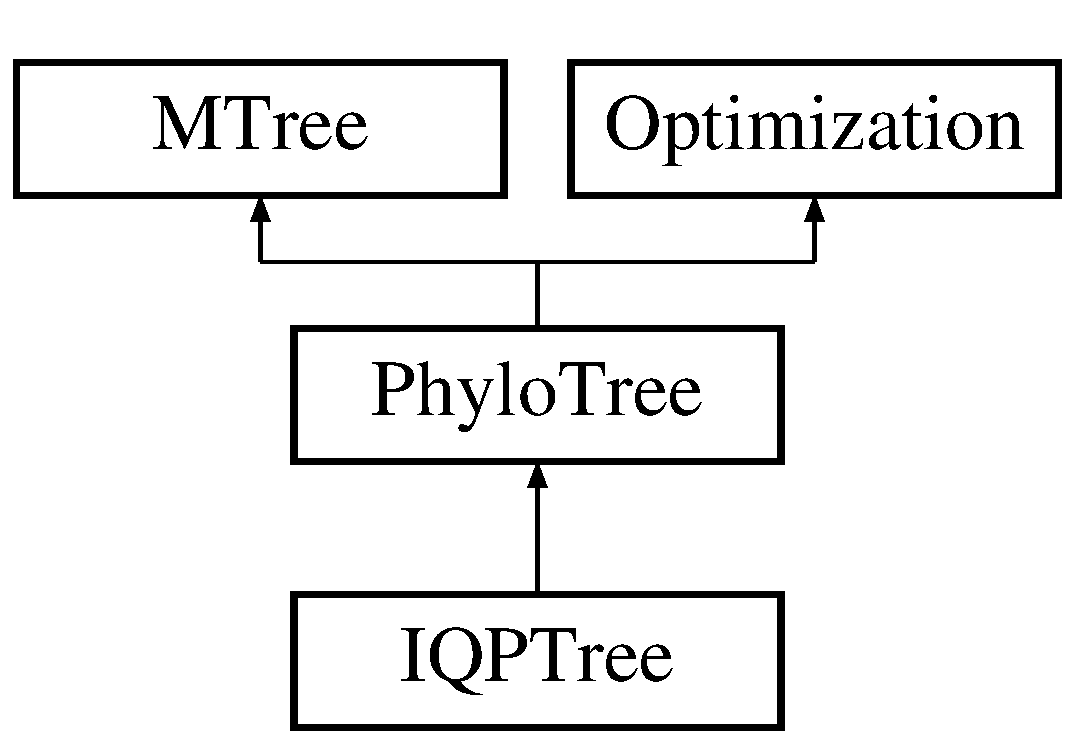
\includegraphics[height=3cm]{classIQPTree}
\end{center}
\end{figure}
\subsection*{Public Member Functions}
\begin{DoxyCompactItemize}
\item 
\hyperlink{classIQPTree_aa29641a82fd24a3023b527496b1d1903}{IQPTree} ()
\item 
virtual \hyperlink{classIQPTree_a35619d9f009df68327f7639ecded27f8}{$\sim$IQPTree} ()
\item 
void \hyperlink{classIQPTree_aa77b4949058eb92e6179f9cfab2330d1}{setRepresentNum} (int k\_\-rep)
\item 
void \hyperlink{classIQPTree_a94b43e66444d6f5d8f6fec75ff708add}{setProbDelete} (double p\_\-del)
\item 
void \hyperlink{classIQPTree_a8e837502069fdce36da52ac029b5f1ff}{setIQPIterations} (int iterations)
\item 
void \hyperlink{classIQPTree_a008a05f575902d53ca355452a8e63082}{findRepresentLeaves} (RepresentLeafSet \&leaves, \hyperlink{classPhyloNode}{PhyloNode} $\ast$node=NULL, \hyperlink{classPhyloNode}{PhyloNode} $\ast$dad=NULL)
\item 
double \hyperlink{classIQPTree_aa7d776139b6b10625fce6bc0cd33274d}{doIQP} ()
\item 
double \hyperlink{classIQPTree_af92cd63a37e644c51bb4006b07a32a53}{doIQPNNI} (string tree\_\-file\_\-name)
\item 
virtual double \hyperlink{classIQPTree_a8d1a63f976a3a219bc8a23ed356e1d65}{optimizeNNI} ()
\end{DoxyCompactItemize}
\subsection*{Public Attributes}
\begin{DoxyCompactItemize}
\item 
double $\ast$ \hyperlink{classIQPTree_a48c7ed5f847b021180e600b1d779c8cb}{dist\_\-matrix}
\end{DoxyCompactItemize}
\subsection*{Protected Member Functions}
\begin{DoxyCompactItemize}
\item 
void \hyperlink{classIQPTree_a2e7b8c974f3d42a09bf652e8683d79f1}{deleteLeaf} (\hyperlink{classNode}{Node} $\ast$leaf)
\item 
void \hyperlink{classIQPTree_a038522be23c6a8fef71a2a1ffa983976}{deleteLeaves} (PhyloNodeVector \&del\_\-leaves, PhyloNodeVector \&adjacent\_\-nodes)
\item 
void \hyperlink{classIQPTree_ad6adbd783583faa754deb9c6d15eb93f}{reinsertLeaf} (\hyperlink{classNode}{Node} $\ast$leaf, \hyperlink{classNode}{Node} $\ast$adjacent\_\-node, \hyperlink{classNode}{Node} $\ast$node, \hyperlink{classNode}{Node} $\ast$dad)
\item 
void \hyperlink{classIQPTree_a803d8f087733ff4c7d4b400c87b35cea}{reinsertLeaves} (PhyloNodeVector \&del\_\-leaves, PhyloNodeVector \&adjacent\_\-nodes)
\item 
int \hyperlink{classIQPTree_ac33ea4963fb4d0ae1ba3e9df424aa7bc}{assessQuartet} (\hyperlink{classNode}{Node} $\ast$leaf0, \hyperlink{classNode}{Node} $\ast$leaf1, \hyperlink{classNode}{Node} $\ast$leaf2, \hyperlink{classNode}{Node} $\ast$del\_\-leaf)
\item 
void \hyperlink{classIQPTree_a5d319c525a15c21f9956fcae5e9d0884}{assessQuartets} (\hyperlink{classPhyloNode}{PhyloNode} $\ast$cur\_\-root, \hyperlink{classPhyloNode}{PhyloNode} $\ast$del\_\-leaf)
\item 
void \hyperlink{classIQPTree_ad617c01926a2efbdf1c64b025edddccc}{initializeBonus} ()
\item 
void \hyperlink{classIQPTree_a72733c572a34fce5483d9c58fddc54d1}{raiseBonus} (\hyperlink{classNode}{Node} $\ast$node, \hyperlink{classNode}{Node} $\ast$dad)
\item 
double \hyperlink{classIQPTree_a96cbd6e8fa106324e176fa15c6c7e77a}{findBestBonus} (\hyperlink{classNode}{Node} $\ast$node, \hyperlink{classNode}{Node} $\ast$dad, \hyperlink{classNode}{Node} $\ast$\&best\_\-node, \hyperlink{classNode}{Node} $\ast$\&best\_\-dad)
\end{DoxyCompactItemize}
\subsection*{Protected Attributes}
\begin{DoxyCompactItemize}
\item 
int \hyperlink{classIQPTree_a3ee6ae6c50af3a0bf669e7f550a5d670}{k\_\-represent}
\item 
double \hyperlink{classIQPTree_a74e9e5f5ce563559d2788818f0584459}{p\_\-delete}
\item 
int \hyperlink{classIQPTree_aee1659fac7169d2adca3e9b2609b638e}{iqpnni\_\-iterations}
\item 
double $\ast$ \hyperlink{classIQPTree_ae9f6d55e262018addddb737f16ca1bd5}{bonus\_\-values}
\end{DoxyCompactItemize}


\subsection{Detailed Description}
Important Quartet Puzzling

\begin{DoxyAuthor}{Author}
BUI Quang Minh $<$\href{mailto:minh.bui@univie.ac.at}{\tt minh.bui@univie.ac.at}$>$ 
\end{DoxyAuthor}


\subsection{Constructor \& Destructor Documentation}
\hypertarget{classIQPTree_aa29641a82fd24a3023b527496b1d1903}{
\index{IQPTree@{IQPTree}!IQPTree@{IQPTree}}
\index{IQPTree@{IQPTree}!IQPTree@{IQPTree}}
\subsubsection[{IQPTree}]{\setlength{\rightskip}{0pt plus 5cm}IQPTree::IQPTree ()}}
\label{classIQPTree_aa29641a82fd24a3023b527496b1d1903}
constructor \hypertarget{classIQPTree_a35619d9f009df68327f7639ecded27f8}{
\index{IQPTree@{IQPTree}!$\sim$IQPTree@{$\sim$IQPTree}}
\index{$\sim$IQPTree@{$\sim$IQPTree}!IQPTree@{IQPTree}}
\subsubsection[{$\sim$IQPTree}]{\setlength{\rightskip}{0pt plus 5cm}IQPTree::$\sim$IQPTree ()\hspace{0.3cm}{\ttfamily  \mbox{[}virtual\mbox{]}}}}
\label{classIQPTree_a35619d9f009df68327f7639ecded27f8}
destructor 

\subsection{Member Function Documentation}
\hypertarget{classIQPTree_ac33ea4963fb4d0ae1ba3e9df424aa7bc}{
\index{IQPTree@{IQPTree}!assessQuartet@{assessQuartet}}
\index{assessQuartet@{assessQuartet}!IQPTree@{IQPTree}}
\subsubsection[{assessQuartet}]{\setlength{\rightskip}{0pt plus 5cm}int IQPTree::assessQuartet ({\bf Node} $\ast$ {\em leaf0}, \/  {\bf Node} $\ast$ {\em leaf1}, \/  {\bf Node} $\ast$ {\em leaf2}, \/  {\bf Node} $\ast$ {\em del\_\-leaf})\hspace{0.3cm}{\ttfamily  \mbox{[}protected\mbox{]}}}}
\label{classIQPTree_ac33ea4963fb4d0ae1ba3e9df424aa7bc}
assess a quartet with four taxa. Current implementation uses the four-\/point condition based on distance matrix for quick evaluation. 
\begin{DoxyParams}{Parameters}
\item[{\em leaf0}]one of the leaf in the existing sub-\/tree \item[{\em leaf1}]one of the leaf in the existing sub-\/tree \item[{\em leaf2}]one of the leaf in the existing sub-\/tree \item[{\em del\_\-leaf}]a leaf that was deleted (not in the existing sub-\/tree) \end{DoxyParams}
\hypertarget{classIQPTree_a5d319c525a15c21f9956fcae5e9d0884}{
\index{IQPTree@{IQPTree}!assessQuartets@{assessQuartets}}
\index{assessQuartets@{assessQuartets}!IQPTree@{IQPTree}}
\subsubsection[{assessQuartets}]{\setlength{\rightskip}{0pt plus 5cm}void IQPTree::assessQuartets ({\bf PhyloNode} $\ast$ {\em cur\_\-root}, \/  {\bf PhyloNode} $\ast$ {\em del\_\-leaf})\hspace{0.3cm}{\ttfamily  \mbox{[}protected\mbox{]}}}}
\label{classIQPTree_a5d319c525a15c21f9956fcae5e9d0884}
assess the important quartets around a virtual root of the tree. This function will assign bonus points to branches by updating the variable 'bonus\_\-values' 
\begin{DoxyParams}{Parameters}
\item[{\em cur\_\-root}]the current virtual root \item[{\em del\_\-leaf}]a leaf that was deleted (not in the existing sub-\/tree) \end{DoxyParams}
\hypertarget{classIQPTree_a2e7b8c974f3d42a09bf652e8683d79f1}{
\index{IQPTree@{IQPTree}!deleteLeaf@{deleteLeaf}}
\index{deleteLeaf@{deleteLeaf}!IQPTree@{IQPTree}}
\subsubsection[{deleteLeaf}]{\setlength{\rightskip}{0pt plus 5cm}void IQPTree::deleteLeaf ({\bf Node} $\ast$ {\em leaf})\hspace{0.3cm}{\ttfamily  \mbox{[}protected\mbox{]}}}}
\label{classIQPTree_a2e7b8c974f3d42a09bf652e8683d79f1}
delete a leaf from the tree, assume tree is birfucating 
\begin{DoxyParams}{Parameters}
\item[{\em leaf}]the leaf node to remove \end{DoxyParams}
\hypertarget{classIQPTree_a038522be23c6a8fef71a2a1ffa983976}{
\index{IQPTree@{IQPTree}!deleteLeaves@{deleteLeaves}}
\index{deleteLeaves@{deleteLeaves}!IQPTree@{IQPTree}}
\subsubsection[{deleteLeaves}]{\setlength{\rightskip}{0pt plus 5cm}void IQPTree::deleteLeaves (PhyloNodeVector \& {\em del\_\-leaves}, \/  PhyloNodeVector \& {\em adjacent\_\-nodes})\hspace{0.3cm}{\ttfamily  \mbox{[}protected\mbox{]}}}}
\label{classIQPTree_a038522be23c6a8fef71a2a1ffa983976}
delete a set of leaves from tree (with the probability p\_\-delete), assume tree is birfucating 
\begin{DoxyParams}{Parameters}
\item[{\em del\_\-leaves}](OUT) the list of deleted leaves \item[{\em adjacent\_\-nodes}](OUT) the corresponding list of nodes adjacent to the deleted leaves \end{DoxyParams}
\hypertarget{classIQPTree_aa7d776139b6b10625fce6bc0cd33274d}{
\index{IQPTree@{IQPTree}!doIQP@{doIQP}}
\index{doIQP@{doIQP}!IQPTree@{IQPTree}}
\subsubsection[{doIQP}]{\setlength{\rightskip}{0pt plus 5cm}double IQPTree::doIQP ()}}
\label{classIQPTree_aa7d776139b6b10625fce6bc0cd33274d}
perform one IQPNNI iteration \begin{DoxyReturn}{Returns}
current likelihood 
\end{DoxyReturn}
\hypertarget{classIQPTree_af92cd63a37e644c51bb4006b07a32a53}{
\index{IQPTree@{IQPTree}!doIQPNNI@{doIQPNNI}}
\index{doIQPNNI@{doIQPNNI}!IQPTree@{IQPTree}}
\subsubsection[{doIQPNNI}]{\setlength{\rightskip}{0pt plus 5cm}double IQPTree::doIQPNNI (string {\em tree\_\-file\_\-name})}}
\label{classIQPTree_af92cd63a37e644c51bb4006b07a32a53}
perform all IQPNNI iterations \begin{DoxyReturn}{Returns}
best likelihood found 
\end{DoxyReturn}

\begin{DoxyParams}{Parameters}
\item[{\em tree\_\-file\_\-name}]name of the tree file to write the best tree found \end{DoxyParams}
\hypertarget{classIQPTree_a96cbd6e8fa106324e176fa15c6c7e77a}{
\index{IQPTree@{IQPTree}!findBestBonus@{findBestBonus}}
\index{findBestBonus@{findBestBonus}!IQPTree@{IQPTree}}
\subsubsection[{findBestBonus}]{\setlength{\rightskip}{0pt plus 5cm}double IQPTree::findBestBonus ({\bf Node} $\ast$ {\em node}, \/  {\bf Node} $\ast$ {\em dad}, \/  {\bf Node} $\ast$\& {\em best\_\-node}, \/  {\bf Node} $\ast$\& {\em best\_\-dad})\hspace{0.3cm}{\ttfamily  \mbox{[}protected\mbox{]}}}}
\label{classIQPTree_a96cbd6e8fa106324e176fa15c6c7e77a}
find the branch with the best bonus points 
\begin{DoxyParams}{Parameters}
\item[{\em node}]the root of the sub-\/tree \item[{\em dad}]dad of 'node', used to direct the recursion \item[{\em best\_\-node}](OUT) one end of the branch with highest bonus point \item[{\em best\_\-dad}](OUT) the other end of the branch with highest bonus point \end{DoxyParams}
\hypertarget{classIQPTree_a008a05f575902d53ca355452a8e63082}{
\index{IQPTree@{IQPTree}!findRepresentLeaves@{findRepresentLeaves}}
\index{findRepresentLeaves@{findRepresentLeaves}!IQPTree@{IQPTree}}
\subsubsection[{findRepresentLeaves}]{\setlength{\rightskip}{0pt plus 5cm}void IQPTree::findRepresentLeaves (RepresentLeafSet \& {\em leaves}, \/  {\bf PhyloNode} $\ast$ {\em node} = {\ttfamily NULL}, \/  {\bf PhyloNode} $\ast$ {\em dad} = {\ttfamily NULL})}}
\label{classIQPTree_a008a05f575902d53ca355452a8e63082}
find the k-\/representative leaves under the node 
\begin{DoxyParams}{Parameters}
\item[{\em node}]the node at which the subtree is rooted \item[{\em dad}]the dad node of the considered subtree, to direct the search \item[{\em leaves}](OUT) the k-\/representative leaf set \end{DoxyParams}
\hypertarget{classIQPTree_ad617c01926a2efbdf1c64b025edddccc}{
\index{IQPTree@{IQPTree}!initializeBonus@{initializeBonus}}
\index{initializeBonus@{initializeBonus}!IQPTree@{IQPTree}}
\subsubsection[{initializeBonus}]{\setlength{\rightskip}{0pt plus 5cm}void IQPTree::initializeBonus ()\hspace{0.3cm}{\ttfamily  \mbox{[}protected\mbox{]}}}}
\label{classIQPTree_ad617c01926a2efbdf1c64b025edddccc}
initialize the bonus points to ZERO \hypertarget{classIQPTree_a8d1a63f976a3a219bc8a23ed356e1d65}{
\index{IQPTree@{IQPTree}!optimizeNNI@{optimizeNNI}}
\index{optimizeNNI@{optimizeNNI}!IQPTree@{IQPTree}}
\subsubsection[{optimizeNNI}]{\setlength{\rightskip}{0pt plus 5cm}double IQPTree::optimizeNNI ()\hspace{0.3cm}{\ttfamily  \mbox{[}virtual\mbox{]}}}}
\label{classIQPTree_a8d1a63f976a3a219bc8a23ed356e1d65}
This implement the fastNNI algorithm proposed in PHYML paper TUNG: this is a virtual function, so it will be called automatically by \hyperlink{classPhyloTree_acef313906a2021de5de2eb87226a202d}{optimizeNNIBranches()} \begin{DoxyReturn}{Returns}
best likelihood found 
\end{DoxyReturn}


Reimplemented from \hyperlink{classPhyloTree_a8927dbf75a06ea797cc76b619759985d}{PhyloTree}.\hypertarget{classIQPTree_a72733c572a34fce5483d9c58fddc54d1}{
\index{IQPTree@{IQPTree}!raiseBonus@{raiseBonus}}
\index{raiseBonus@{raiseBonus}!IQPTree@{IQPTree}}
\subsubsection[{raiseBonus}]{\setlength{\rightskip}{0pt plus 5cm}void IQPTree::raiseBonus ({\bf Node} $\ast$ {\em node}, \/  {\bf Node} $\ast$ {\em dad})\hspace{0.3cm}{\ttfamily  \mbox{[}protected\mbox{]}}}}
\label{classIQPTree_a72733c572a34fce5483d9c58fddc54d1}
raise the bonus points for all branches in the subtree rooted at a node 
\begin{DoxyParams}{Parameters}
\item[{\em node}]the root of the sub-\/tree \item[{\em dad}]dad of 'node', used to direct the recursion \end{DoxyParams}
\hypertarget{classIQPTree_ad6adbd783583faa754deb9c6d15eb93f}{
\index{IQPTree@{IQPTree}!reinsertLeaf@{reinsertLeaf}}
\index{reinsertLeaf@{reinsertLeaf}!IQPTree@{IQPTree}}
\subsubsection[{reinsertLeaf}]{\setlength{\rightskip}{0pt plus 5cm}void IQPTree::reinsertLeaf ({\bf Node} $\ast$ {\em leaf}, \/  {\bf Node} $\ast$ {\em adjacent\_\-node}, \/  {\bf Node} $\ast$ {\em node}, \/  {\bf Node} $\ast$ {\em dad})\hspace{0.3cm}{\ttfamily  \mbox{[}protected\mbox{]}}}}
\label{classIQPTree_ad6adbd783583faa754deb9c6d15eb93f}
reinsert one leaf back into the tree 
\begin{DoxyParams}{Parameters}
\item[{\em leaf}]the leaf to reinsert \item[{\em adjacent\_\-node}]the node adjacent to the leaf, returned by \hyperlink{classIQPTree_a038522be23c6a8fef71a2a1ffa983976}{deleteLeaves()} funcrion \item[{\em node}]one end node of the reinsertion branch in the existing tree \item[{\em dad}]the other node of the reinsertion branch in the existing tree \end{DoxyParams}
\hypertarget{classIQPTree_a803d8f087733ff4c7d4b400c87b35cea}{
\index{IQPTree@{IQPTree}!reinsertLeaves@{reinsertLeaves}}
\index{reinsertLeaves@{reinsertLeaves}!IQPTree@{IQPTree}}
\subsubsection[{reinsertLeaves}]{\setlength{\rightskip}{0pt plus 5cm}void IQPTree::reinsertLeaves (PhyloNodeVector \& {\em del\_\-leaves}, \/  PhyloNodeVector \& {\em adjacent\_\-nodes})\hspace{0.3cm}{\ttfamily  \mbox{[}protected\mbox{]}}}}
\label{classIQPTree_a803d8f087733ff4c7d4b400c87b35cea}
reinsert the whole list of leaves back into the tree 
\begin{DoxyParams}{Parameters}
\item[{\em del\_\-leaves}]the list of deleted leaves, returned by \hyperlink{classIQPTree_a038522be23c6a8fef71a2a1ffa983976}{deleteLeaves()} function \item[{\em adjacent\_\-nodes}]the corresponding list of nodes adjacent to the deleted leaves, returned by \hyperlink{classIQPTree_a038522be23c6a8fef71a2a1ffa983976}{deleteLeaves()} function \end{DoxyParams}
\hypertarget{classIQPTree_a8e837502069fdce36da52ac029b5f1ff}{
\index{IQPTree@{IQPTree}!setIQPIterations@{setIQPIterations}}
\index{setIQPIterations@{setIQPIterations}!IQPTree@{IQPTree}}
\subsubsection[{setIQPIterations}]{\setlength{\rightskip}{0pt plus 5cm}void IQPTree::setIQPIterations (int {\em iterations})}}
\label{classIQPTree_a8e837502069fdce36da52ac029b5f1ff}
set the number of iterations for the IQPNNI algorithm 
\begin{DoxyParams}{Parameters}
\item[{\em iterations}]the number of iterations \end{DoxyParams}
\hypertarget{classIQPTree_a94b43e66444d6f5d8f6fec75ff708add}{
\index{IQPTree@{IQPTree}!setProbDelete@{setProbDelete}}
\index{setProbDelete@{setProbDelete}!IQPTree@{IQPTree}}
\subsubsection[{setProbDelete}]{\setlength{\rightskip}{0pt plus 5cm}void IQPTree::setProbDelete (double {\em p\_\-del})}}
\label{classIQPTree_a94b43e66444d6f5d8f6fec75ff708add}
set the probability of deleteing sequences for IQP algorithm 
\begin{DoxyParams}{Parameters}
\item[{\em p\_\-del}]probability of deleting sequences \end{DoxyParams}
\hypertarget{classIQPTree_aa77b4949058eb92e6179f9cfab2330d1}{
\index{IQPTree@{IQPTree}!setRepresentNum@{setRepresentNum}}
\index{setRepresentNum@{setRepresentNum}!IQPTree@{IQPTree}}
\subsubsection[{setRepresentNum}]{\setlength{\rightskip}{0pt plus 5cm}void IQPTree::setRepresentNum (int {\em k\_\-rep})}}
\label{classIQPTree_aa77b4949058eb92e6179f9cfab2330d1}
set k-\/representative parameter 
\begin{DoxyParams}{Parameters}
\item[{\em k\_\-rep}]k-\/representative \end{DoxyParams}


\subsection{Member Data Documentation}
\hypertarget{classIQPTree_ae9f6d55e262018addddb737f16ca1bd5}{
\index{IQPTree@{IQPTree}!bonus\_\-values@{bonus\_\-values}}
\index{bonus\_\-values@{bonus\_\-values}!IQPTree@{IQPTree}}
\subsubsection[{bonus\_\-values}]{\setlength{\rightskip}{0pt plus 5cm}double$\ast$ {\bf IQPTree::bonus\_\-values}\hspace{0.3cm}{\ttfamily  \mbox{[}protected\mbox{]}}}}
\label{classIQPTree_ae9f6d55e262018addddb737f16ca1bd5}
bonus values of all branches, used for IQP algorithm \hypertarget{classIQPTree_a48c7ed5f847b021180e600b1d779c8cb}{
\index{IQPTree@{IQPTree}!dist\_\-matrix@{dist\_\-matrix}}
\index{dist\_\-matrix@{dist\_\-matrix}!IQPTree@{IQPTree}}
\subsubsection[{dist\_\-matrix}]{\setlength{\rightskip}{0pt plus 5cm}double$\ast$ {\bf IQPTree::dist\_\-matrix}}}
\label{classIQPTree_a48c7ed5f847b021180e600b1d779c8cb}
distance matrix, used for IQP algorithm \hypertarget{classIQPTree_aee1659fac7169d2adca3e9b2609b638e}{
\index{IQPTree@{IQPTree}!iqpnni\_\-iterations@{iqpnni\_\-iterations}}
\index{iqpnni\_\-iterations@{iqpnni\_\-iterations}!IQPTree@{IQPTree}}
\subsubsection[{iqpnni\_\-iterations}]{\setlength{\rightskip}{0pt plus 5cm}int {\bf IQPTree::iqpnni\_\-iterations}\hspace{0.3cm}{\ttfamily  \mbox{[}protected\mbox{]}}}}
\label{classIQPTree_aee1659fac7169d2adca3e9b2609b638e}
number of IQPNNI iterations \hypertarget{classIQPTree_a3ee6ae6c50af3a0bf669e7f550a5d670}{
\index{IQPTree@{IQPTree}!k\_\-represent@{k\_\-represent}}
\index{k\_\-represent@{k\_\-represent}!IQPTree@{IQPTree}}
\subsubsection[{k\_\-represent}]{\setlength{\rightskip}{0pt plus 5cm}int {\bf IQPTree::k\_\-represent}\hspace{0.3cm}{\ttfamily  \mbox{[}protected\mbox{]}}}}
\label{classIQPTree_a3ee6ae6c50af3a0bf669e7f550a5d670}
k-\/representative parameter \hypertarget{classIQPTree_a74e9e5f5ce563559d2788818f0584459}{
\index{IQPTree@{IQPTree}!p\_\-delete@{p\_\-delete}}
\index{p\_\-delete@{p\_\-delete}!IQPTree@{IQPTree}}
\subsubsection[{p\_\-delete}]{\setlength{\rightskip}{0pt plus 5cm}double {\bf IQPTree::p\_\-delete}\hspace{0.3cm}{\ttfamily  \mbox{[}protected\mbox{]}}}}
\label{classIQPTree_a74e9e5f5ce563559d2788818f0584459}
probability to delete a leaf 

The documentation for this class was generated from the following files:\begin{DoxyCompactItemize}
\item 
src/iqptree.h\item 
src/iqptree.cpp\end{DoxyCompactItemize}

\hypertarget{structstd_1_1less_3_01Split_01_5_01_4}{
\section{std::less$<$ Split $\ast$ $>$ Struct Template Reference}
\label{structstd_1_1less_3_01Split_01_5_01_4}\index{std::less$<$ Split $\ast$ $>$@{std::less$<$ Split $\ast$ $>$}}
}


{\ttfamily \#include $<$hashsplitset.h$>$}\subsection*{Public Member Functions}
\begin{DoxyCompactItemize}
\item 
bool \hyperlink{structstd_1_1less_3_01Split_01_5_01_4_ac0a084b10fedf41d9459766b5c3a0033}{operator()} (const \hyperlink{classSplit}{Split} $\ast$s1, const \hyperlink{classSplit}{Split} $\ast$s2) const 
\end{DoxyCompactItemize}


\subsection{Detailed Description}
\subsubsection*{template$<$$>$ struct std::less$<$ Split $\ast$ $>$}

Define less than relationship of two splits, used for set (or map) template 

\subsection{Member Function Documentation}
\hypertarget{structstd_1_1less_3_01Split_01_5_01_4_ac0a084b10fedf41d9459766b5c3a0033}{
\index{std::less$<$ Split $\ast$ $>$@{std::less$<$ Split $\ast$ $>$}!operator()@{operator()}}
\index{operator()@{operator()}!std::less< Split * >@{std::less$<$ Split $\ast$ $>$}}
\subsubsection[{operator()}]{\setlength{\rightskip}{0pt plus 5cm}bool std::less$<$ {\bf Split} $\ast$ $>$::operator() (const {\bf Split} $\ast$ {\em s1}, \/  const {\bf Split} $\ast$ {\em s2}) const\hspace{0.3cm}{\ttfamily  \mbox{[}inline\mbox{]}}}}
\label{structstd_1_1less_3_01Split_01_5_01_4_ac0a084b10fedf41d9459766b5c3a0033}
\begin{DoxyReturn}{Returns}
true if $\ast$s1 $<$ $\ast$s2 alphabetically 
\end{DoxyReturn}

\begin{DoxyParams}{Parameters}
\item[{\em s1}]first split \item[{\em s2}]second split \end{DoxyParams}


The documentation for this struct was generated from the following file:\begin{DoxyCompactItemize}
\item 
src/hashsplitset.h\end{DoxyCompactItemize}

\hypertarget{classMExtTree}{
\section{MExtTree Class Reference}
\label{classMExtTree}\index{MExtTree@{MExtTree}}
}


{\ttfamily \#include $<$mexttree.h$>$}Inheritance diagram for MExtTree::\begin{figure}[H]
\begin{center}
\leavevmode
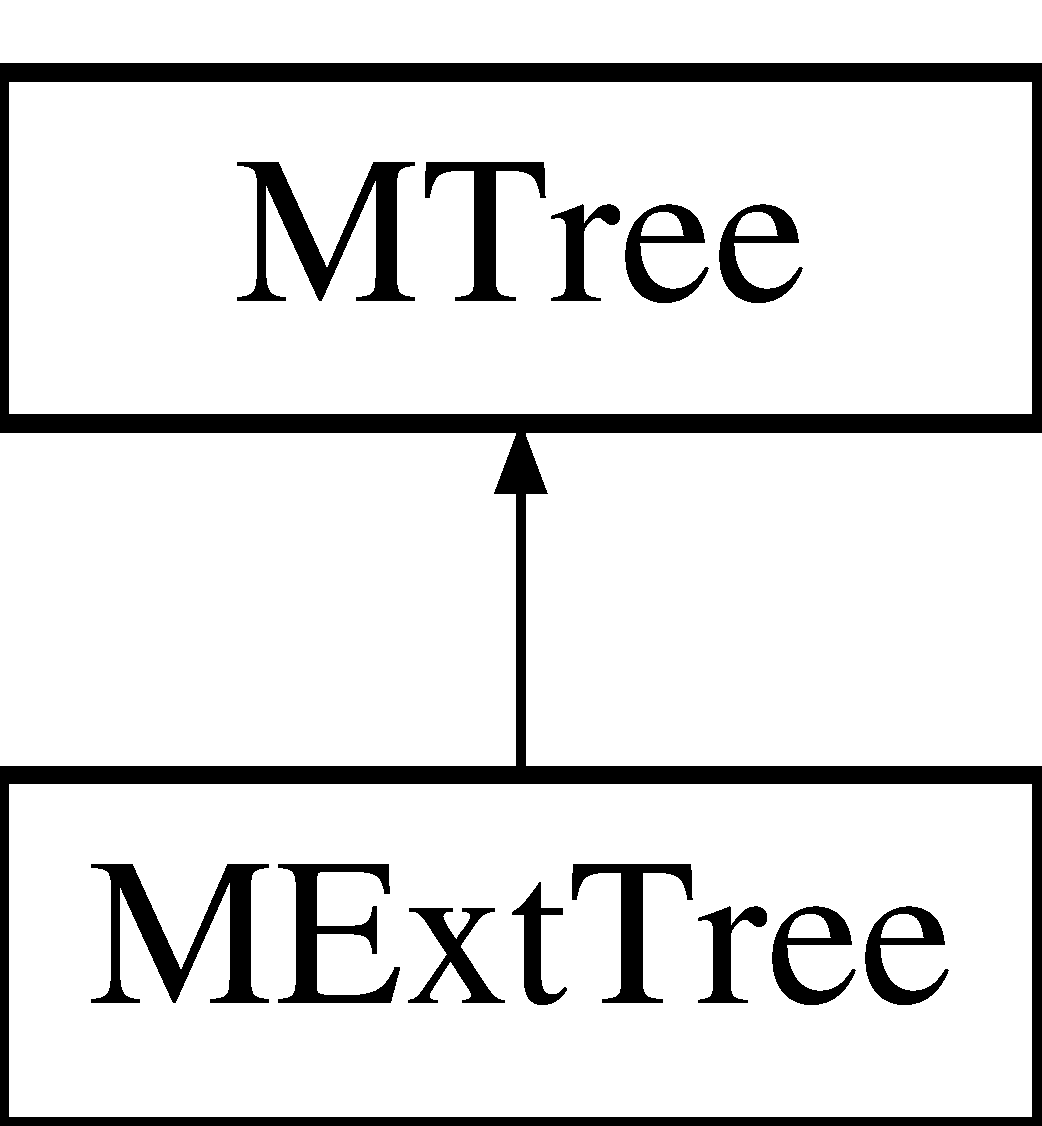
\includegraphics[height=2cm]{classMExtTree}
\end{center}
\end{figure}
\subsection*{Public Member Functions}
\begin{DoxyCompactItemize}
\item 
\hyperlink{classMExtTree_a98519878a9ba52ed6a8b6672666407af}{MExtTree} (const char $\ast$userTreeFile, bool \&is\_\-rooted)
\item 
\hyperlink{classMExtTree_a7a4160a0b7fccfa64ad1e26ceba7774b}{MExtTree} (\hyperlink{classMTree}{MTree} \&tree)
\item 
\hyperlink{classMExtTree_abbad38db501392d69db9544b7f796054}{MExtTree} ()
\item 
void \hyperlink{classMExtTree_aa709714f825099a4128ff8eb0fc3c419}{generateRandomTree} (TreeGenType tree\_\-type, \hyperlink{structParams}{Params} \&params, bool binary=true)
\item 
void \hyperlink{classMExtTree_a9e048ce7a85817ff65dabe6a739ab1d0}{generateYuleHarding} (\hyperlink{structParams}{Params} \&params, bool binary=true)
\item 
void \hyperlink{classMExtTree_a9fa7114ba07c9ae332235e5e2a5baf2b}{generateUniform} (int size, bool binary=true)
\item 
void \hyperlink{classMExtTree_aedaa4579940f46a5a4becde25856d8b4}{generateCaterpillar} (int size)
\item 
void \hyperlink{classMExtTree_aace82df578f02396df24b7dde3ae81bc}{generateBalanced} (int size)
\item 
void \hyperlink{classMExtTree_a690a4da143b341b8969c9d176a221984}{setLeavesName} (NodeVector \&myleaves)
\item 
void \hyperlink{classMExtTree_ab89f62be12aaaf2b63ddbef4e8750b38}{calcDist} (char $\ast$filename)
\item 
void \hyperlink{classMExtTree_a283c7b86a9755f4cc4ec0c9fa7787a48}{calcDist} (matrix(double)\&dist, \hyperlink{classNode}{Node} $\ast$node=NULL, \hyperlink{classNode}{Node} $\ast$dad=NULL)
\item 
void \hyperlink{classMExtTree_a0519ce518addd2ada2794e16436491f3}{calcDist} (\hyperlink{classNode}{Node} $\ast$aroot, double cur\_\-len, matrix(double)\&dist, \hyperlink{classNode}{Node} $\ast$node, \hyperlink{classNode}{Node} $\ast$dad)
\item 
void \hyperlink{classMExtTree_ae1336390c977f7de6153ca2b06e9fbe1}{createBootstrapSupport} (vector$<$ \hyperlink{classNxsString}{NxsString} $>$ \&taxname, \hyperlink{classMTreeSet}{MTreeSet} \&trees, \hyperlink{classSplitGraph}{SplitGraph} \&sg, \hyperlink{classSplitIntMap}{SplitIntMap} \&hash\_\-ss, \hyperlink{classNode}{Node} $\ast$node=NULL, \hyperlink{classNode}{Node} $\ast$dad=NULL)
\item 
\hypertarget{classMExtTree_af47064686e191078090afb640d02fec1}{
void {\bfseries reportDisagreedTrees} (vector$<$ \hyperlink{classNxsString}{NxsString} $>$ \&taxname, \hyperlink{classMTreeSet}{MTreeSet} \&trees, \hyperlink{classSplit}{Split} \&mysplit)}
\label{classMExtTree_af47064686e191078090afb640d02fec1}

\item 
void \hyperlink{classMExtTree_a39d9c5216f1c8cad04b50972a2c83897}{createCluster} (NodeVector \&taxa, matrix(int)\&clusters, \hyperlink{classNode}{Node} $\ast$node=NULL, \hyperlink{classNode}{Node} $\ast$dad=NULL)
\item 
void \hyperlink{classMExtTree_a658a3e1db727b23b7ce67754347230f5}{createCluster} (int clu\_\-num, \hyperlink{classNode}{Node} $\ast$node, \hyperlink{classNode}{Node} $\ast$dad)
\end{DoxyCompactItemize}


\subsection{Detailed Description}
extended tree, for bootstrap, cluster, etc (do not related to PDA main topic)

\begin{DoxyAuthor}{Author}
BUI Quang Minh, Steffen Klaere, Arndt von Haeseler 
\end{DoxyAuthor}


\subsection{Constructor \& Destructor Documentation}
\hypertarget{classMExtTree_a98519878a9ba52ed6a8b6672666407af}{
\index{MExtTree@{MExtTree}!MExtTree@{MExtTree}}
\index{MExtTree@{MExtTree}!MExtTree@{MExtTree}}
\subsubsection[{MExtTree}]{\setlength{\rightskip}{0pt plus 5cm}MExtTree::MExtTree (const char $\ast$ {\em userTreeFile}, \/  bool \& {\em is\_\-rooted})\hspace{0.3cm}{\ttfamily  \mbox{[}inline\mbox{]}}}}
\label{classMExtTree_a98519878a9ba52ed6a8b6672666407af}
constructor, read tree from user file 
\begin{DoxyParams}{Parameters}
\item[{\em userTreeFile}]the name of the user tree \item[{\em is\_\-rooted}](IN/OUT) true if tree is rooted \end{DoxyParams}
\hypertarget{classMExtTree_a7a4160a0b7fccfa64ad1e26ceba7774b}{
\index{MExtTree@{MExtTree}!MExtTree@{MExtTree}}
\index{MExtTree@{MExtTree}!MExtTree@{MExtTree}}
\subsubsection[{MExtTree}]{\setlength{\rightskip}{0pt plus 5cm}MExtTree::MExtTree ({\bf MTree} \& {\em tree})\hspace{0.3cm}{\ttfamily  \mbox{[}inline\mbox{]}}}}
\label{classMExtTree_a7a4160a0b7fccfa64ad1e26ceba7774b}
constructor, get from another tree 
\begin{DoxyParams}{Parameters}
\item[{\em tree}]another \hyperlink{classMTree}{MTree} \end{DoxyParams}
\hypertarget{classMExtTree_abbad38db501392d69db9544b7f796054}{
\index{MExtTree@{MExtTree}!MExtTree@{MExtTree}}
\index{MExtTree@{MExtTree}!MExtTree@{MExtTree}}
\subsubsection[{MExtTree}]{\setlength{\rightskip}{0pt plus 5cm}MExtTree::MExtTree ()\hspace{0.3cm}{\ttfamily  \mbox{[}inline\mbox{]}}}}
\label{classMExtTree_abbad38db501392d69db9544b7f796054}
constructor 

\subsection{Member Function Documentation}
\hypertarget{classMExtTree_a0519ce518addd2ada2794e16436491f3}{
\index{MExtTree@{MExtTree}!calcDist@{calcDist}}
\index{calcDist@{calcDist}!MExtTree@{MExtTree}}
\subsubsection[{calcDist}]{\setlength{\rightskip}{0pt plus 5cm}void MExtTree::calcDist ({\bf Node} $\ast$ {\em aroot}, \/  double {\em cur\_\-len}, \/  matrix(double)\& {\em dist}, \/  {\bf Node} $\ast$ {\em node}, \/  {\bf Node} $\ast$ {\em dad})}}
\label{classMExtTree_a0519ce518addd2ada2794e16436491f3}
calculate the pairwise distances on the tree 
\begin{DoxyParams}{Parameters}
\item[{\em aroot}]the starting root \item[{\em node}]the starting node, NULL to start from the root \item[{\em dad}]dad of the node, used to direct the search \item[{\em cur\_\-len}]current length from aroot to node \item[{\em dist}](OUT) distance matrix \end{DoxyParams}
\hypertarget{classMExtTree_a283c7b86a9755f4cc4ec0c9fa7787a48}{
\index{MExtTree@{MExtTree}!calcDist@{calcDist}}
\index{calcDist@{calcDist}!MExtTree@{MExtTree}}
\subsubsection[{calcDist}]{\setlength{\rightskip}{0pt plus 5cm}void MExtTree::calcDist (matrix(double)\& {\em dist}, \/  {\bf Node} $\ast$ {\em node} = {\ttfamily NULL}, \/  {\bf Node} $\ast$ {\em dad} = {\ttfamily NULL})}}
\label{classMExtTree_a283c7b86a9755f4cc4ec0c9fa7787a48}
calculate the pairwise distances on the tree 
\begin{DoxyParams}{Parameters}
\item[{\em node}]the starting node, NULL to start from the root \item[{\em dad}]dad of the node, used to direct the search \item[{\em dist}](OUT) distance matrix \end{DoxyParams}
\hypertarget{classMExtTree_ab89f62be12aaaf2b63ddbef4e8750b38}{
\index{MExtTree@{MExtTree}!calcDist@{calcDist}}
\index{calcDist@{calcDist}!MExtTree@{MExtTree}}
\subsubsection[{calcDist}]{\setlength{\rightskip}{0pt plus 5cm}void MExtTree::calcDist (char $\ast$ {\em filename})}}
\label{classMExtTree_ab89f62be12aaaf2b63ddbef4e8750b38}
calculate the pairwise distances on the tree, print the matrix to file (in phylip format) 
\begin{DoxyParams}{Parameters}
\item[{\em filename}]file name \end{DoxyParams}
\hypertarget{classMExtTree_ae1336390c977f7de6153ca2b06e9fbe1}{
\index{MExtTree@{MExtTree}!createBootstrapSupport@{createBootstrapSupport}}
\index{createBootstrapSupport@{createBootstrapSupport}!MExtTree@{MExtTree}}
\subsubsection[{createBootstrapSupport}]{\setlength{\rightskip}{0pt plus 5cm}void MExtTree::createBootstrapSupport (vector$<$ {\bf NxsString} $>$ \& {\em taxname}, \/  {\bf MTreeSet} \& {\em trees}, \/  {\bf SplitGraph} \& {\em sg}, \/  {\bf SplitIntMap} \& {\em hash\_\-ss}, \/  {\bf Node} $\ast$ {\em node} = {\ttfamily NULL}, \/  {\bf Node} $\ast$ {\em dad} = {\ttfamily NULL})}}
\label{classMExtTree_ae1336390c977f7de6153ca2b06e9fbe1}
create support value for each internal node to the weight of split in the split graph 
\begin{DoxyParams}{Parameters}
\item[{\em node}]the starting node, NULL to start from the root \item[{\em dad}]dad of the node, used to direct the search \item[{\em sg}]split graph \item[{\em hash\_\-ss}]hash split set \item[{\em taxname}]vector of taxa names \item[{\em trees}]set of trees \end{DoxyParams}
\hypertarget{classMExtTree_a658a3e1db727b23b7ce67754347230f5}{
\index{MExtTree@{MExtTree}!createCluster@{createCluster}}
\index{createCluster@{createCluster}!MExtTree@{MExtTree}}
\subsubsection[{createCluster}]{\setlength{\rightskip}{0pt plus 5cm}void MExtTree::createCluster (int {\em clu\_\-num}, \/  {\bf Node} $\ast$ {\em node}, \/  {\bf Node} $\ast$ {\em dad})}}
\label{classMExtTree_a658a3e1db727b23b7ce67754347230f5}
create CLUSTER for each branch, useful for likelihood mapping analysis 
\begin{DoxyParams}{Parameters}
\item[{\em clu\_\-num}]cluster number \item[{\em node}]the starting node, NULL to start from the root \item[{\em dad}]dad of the node, used to direct the search \end{DoxyParams}
\hypertarget{classMExtTree_a39d9c5216f1c8cad04b50972a2c83897}{
\index{MExtTree@{MExtTree}!createCluster@{createCluster}}
\index{createCluster@{createCluster}!MExtTree@{MExtTree}}
\subsubsection[{createCluster}]{\setlength{\rightskip}{0pt plus 5cm}void MExtTree::createCluster (NodeVector \& {\em taxa}, \/  matrix(int)\& {\em clusters}, \/  {\bf Node} $\ast$ {\em node} = {\ttfamily NULL}, \/  {\bf Node} $\ast$ {\em dad} = {\ttfamily NULL})}}
\label{classMExtTree_a39d9c5216f1c8cad04b50972a2c83897}
create CLUSTER for each branch, useful for likelihood mapping analysis 
\begin{DoxyParams}{Parameters}
\item[{\em taxa}]an order of taxa \item[{\em clusters}](OUT) list of all clusters \item[{\em node}]the starting node, NULL to start from the root \item[{\em dad}]dad of the node, used to direct the search \end{DoxyParams}
\hypertarget{classMExtTree_aace82df578f02396df24b7dde3ae81bc}{
\index{MExtTree@{MExtTree}!generateBalanced@{generateBalanced}}
\index{generateBalanced@{generateBalanced}!MExtTree@{MExtTree}}
\subsubsection[{generateBalanced}]{\setlength{\rightskip}{0pt plus 5cm}void MExtTree::generateBalanced (int {\em size})}}
\label{classMExtTree_aace82df578f02396df24b7dde3ae81bc}
generate a balanced tree 
\begin{DoxyParams}{Parameters}
\item[{\em size}]number of taxa \end{DoxyParams}
\hypertarget{classMExtTree_aedaa4579940f46a5a4becde25856d8b4}{
\index{MExtTree@{MExtTree}!generateCaterpillar@{generateCaterpillar}}
\index{generateCaterpillar@{generateCaterpillar}!MExtTree@{MExtTree}}
\subsubsection[{generateCaterpillar}]{\setlength{\rightskip}{0pt plus 5cm}void MExtTree::generateCaterpillar (int {\em size})}}
\label{classMExtTree_aedaa4579940f46a5a4becde25856d8b4}
generate a caterpillar tree 
\begin{DoxyParams}{Parameters}
\item[{\em size}]number of taxa \end{DoxyParams}
\hypertarget{classMExtTree_aa709714f825099a4128ff8eb0fc3c419}{
\index{MExtTree@{MExtTree}!generateRandomTree@{generateRandomTree}}
\index{generateRandomTree@{generateRandomTree}!MExtTree@{MExtTree}}
\subsubsection[{generateRandomTree}]{\setlength{\rightskip}{0pt plus 5cm}void MExtTree::generateRandomTree (TreeGenType {\em tree\_\-type}, \/  {\bf Params} \& {\em params}, \/  bool {\em binary} = {\ttfamily true})}}
\label{classMExtTree_aa709714f825099a4128ff8eb0fc3c419}
generate a random tree with given tree type 
\begin{DoxyParams}{Parameters}
\item[{\em tree\_\-type}]can be YULE\_\-HARDING, UNIFORM, BALANCED, or CATERPILLAR \item[{\em params}]program parameters \item[{\em binary}]TRUE if you want to generate a binary tree \end{DoxyParams}
\hypertarget{classMExtTree_a9fa7114ba07c9ae332235e5e2a5baf2b}{
\index{MExtTree@{MExtTree}!generateUniform@{generateUniform}}
\index{generateUniform@{generateUniform}!MExtTree@{MExtTree}}
\subsubsection[{generateUniform}]{\setlength{\rightskip}{0pt plus 5cm}void MExtTree::generateUniform (int {\em size}, \/  bool {\em binary} = {\ttfamily true})}}
\label{classMExtTree_a9fa7114ba07c9ae332235e5e2a5baf2b}
generate a random tree following uniform model 
\begin{DoxyParams}{Parameters}
\item[{\em size}]number of taxa \item[{\em binary}]TRUE if you want to generate a binary tree\end{DoxyParams}
generate a random tree following uniform model \hypertarget{classMExtTree_a9e048ce7a85817ff65dabe6a739ab1d0}{
\index{MExtTree@{MExtTree}!generateYuleHarding@{generateYuleHarding}}
\index{generateYuleHarding@{generateYuleHarding}!MExtTree@{MExtTree}}
\subsubsection[{generateYuleHarding}]{\setlength{\rightskip}{0pt plus 5cm}void MExtTree::generateYuleHarding ({\bf Params} \& {\em params}, \/  bool {\em binary} = {\ttfamily true})}}
\label{classMExtTree_a9e048ce7a85817ff65dabe6a739ab1d0}
generate a random tree following Yule-\/Harding model 
\begin{DoxyParams}{Parameters}
\item[{\em params}]program parameters \item[{\em binary}]TRUE if you want to generate a binary tree\end{DoxyParams}
generate a random tree following Yule Harding model \hypertarget{classMExtTree_a690a4da143b341b8969c9d176a221984}{
\index{MExtTree@{MExtTree}!setLeavesName@{setLeavesName}}
\index{setLeavesName@{setLeavesName}!MExtTree@{MExtTree}}
\subsubsection[{setLeavesName}]{\setlength{\rightskip}{0pt plus 5cm}void MExtTree::setLeavesName (NodeVector \& {\em myleaves})}}
\label{classMExtTree_a690a4da143b341b8969c9d176a221984}
set the leaf ID and names when generating random tree 
\begin{DoxyParams}{Parameters}
\item[{\em myleaves}]vector of leaves \end{DoxyParams}


The documentation for this class was generated from the following files:\begin{DoxyCompactItemize}
\item 
src/mexttree.h\item 
src/mexttree.cpp\end{DoxyCompactItemize}

\hypertarget{classModelDNA}{
\section{ModelDNA Class Reference}
\label{classModelDNA}\index{ModelDNA@{ModelDNA}}
}


{\ttfamily \#include $<$modeldna.h$>$}Inheritance diagram for ModelDNA::\begin{figure}[H]
\begin{center}
\leavevmode
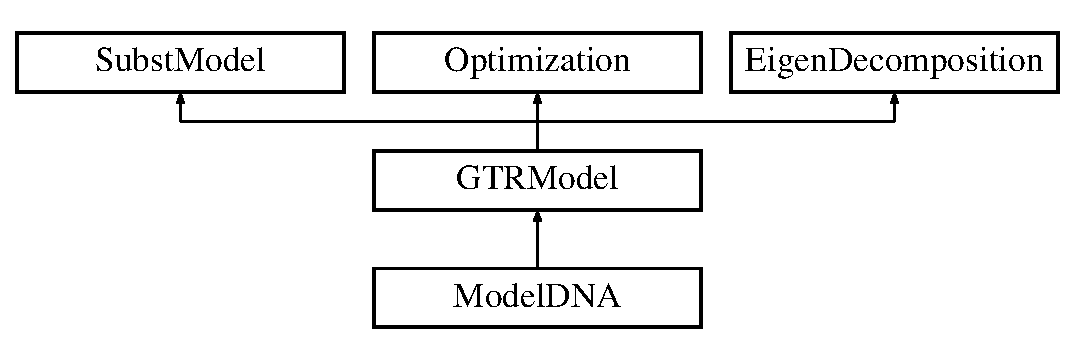
\includegraphics[height=3cm]{classModelDNA}
\end{center}
\end{figure}
\subsection*{Public Member Functions}
\begin{DoxyCompactItemize}
\item 
\hyperlink{classModelDNA_a58ee74d1a55b85db517f65bfa865b4c6}{ModelDNA} (const char $\ast$model\_\-name, StateFreqType freq, \hyperlink{classPhyloTree}{PhyloTree} $\ast$tree)
\item 
virtual void \hyperlink{classModelDNA_ad7f5b56ae6499a222c01ad81e92e27a2}{init} (const char $\ast$model\_\-name, StateFreqType freq)
\item 
void \hyperlink{classModelDNA_a2a44458bfe1d673b6718f2b881682cee}{setRateType} (const char $\ast$rate\_\-spec)
\item 
virtual int \hyperlink{classModelDNA_adc73fda51fb0f02049ed891b29c3a951}{getNDim} ()
\item 
virtual void \hyperlink{classModelDNA_a46a8fd333239a3937e6116608e20cc78}{writeParameters} (ostream \&out)
\end{DoxyCompactItemize}
\subsection*{Protected Member Functions}
\begin{DoxyCompactItemize}
\item 
virtual void \hyperlink{classModelDNA_a83af5938f0b38371b6b971931b8748c2}{setVariables} (double $\ast$variables)
\item 
virtual void \hyperlink{classModelDNA_a4083dfee9b55936019483c5e9a4bb2f7}{getVariables} (double $\ast$variables)
\end{DoxyCompactItemize}
\subsection*{Protected Attributes}
\begin{DoxyCompactItemize}
\item 
string \hyperlink{classModelDNA_a519992726b2a06ec784c036aef64e749}{param\_\-spec}
\item 
int \hyperlink{classModelDNA_acb20f55e922b675d5eb110907fe97ea6}{num\_\-params}
\end{DoxyCompactItemize}


\subsection{Detailed Description}
All DNA models are managed here

\begin{DoxyAuthor}{Author}
BUI Quang Minh $<$\href{mailto:minh.bui@univie.ac.at}{\tt minh.bui@univie.ac.at}$>$ 
\end{DoxyAuthor}


\subsection{Constructor \& Destructor Documentation}
\hypertarget{classModelDNA_a58ee74d1a55b85db517f65bfa865b4c6}{
\index{ModelDNA@{ModelDNA}!ModelDNA@{ModelDNA}}
\index{ModelDNA@{ModelDNA}!ModelDNA@{ModelDNA}}
\subsubsection[{ModelDNA}]{\setlength{\rightskip}{0pt plus 5cm}ModelDNA::ModelDNA (const char $\ast$ {\em model\_\-name}, \/  StateFreqType {\em freq}, \/  {\bf PhyloTree} $\ast$ {\em tree})}}
\label{classModelDNA_a58ee74d1a55b85db517f65bfa865b4c6}
constructor 
\begin{DoxyParams}{Parameters}
\item[{\em model\_\-name}]model name, e.g., JC, HKY. \item[{\em freq}]state frequency type \item[{\em tree}]associated phylogenetic tree \end{DoxyParams}


\subsection{Member Function Documentation}
\hypertarget{classModelDNA_adc73fda51fb0f02049ed891b29c3a951}{
\index{ModelDNA@{ModelDNA}!getNDim@{getNDim}}
\index{getNDim@{getNDim}!ModelDNA@{ModelDNA}}
\subsubsection[{getNDim}]{\setlength{\rightskip}{0pt plus 5cm}int ModelDNA::getNDim ()\hspace{0.3cm}{\ttfamily  \mbox{[}virtual\mbox{]}}}}
\label{classModelDNA_adc73fda51fb0f02049ed891b29c3a951}
return the number of dimensions 

Reimplemented from \hyperlink{classGTRModel_a6e2066898fbbb245596d4a97dd8ee33c}{GTRModel}.\hypertarget{classModelDNA_a4083dfee9b55936019483c5e9a4bb2f7}{
\index{ModelDNA@{ModelDNA}!getVariables@{getVariables}}
\index{getVariables@{getVariables}!ModelDNA@{ModelDNA}}
\subsubsection[{getVariables}]{\setlength{\rightskip}{0pt plus 5cm}void ModelDNA::getVariables (double $\ast$ {\em variables})\hspace{0.3cm}{\ttfamily  \mbox{[}protected, virtual\mbox{]}}}}
\label{classModelDNA_a4083dfee9b55936019483c5e9a4bb2f7}
this function is served for the multi-\/dimension optimization. It should assign the model parameters from a vector of variables that is index from 1 (NOTE: not from 0) 
\begin{DoxyParams}{Parameters}
\item[{\em variables}]vector of variables, indexed from 1 \end{DoxyParams}


Reimplemented from \hyperlink{classGTRModel_ae0d291e293dd142d41466650539a2481}{GTRModel}.\hypertarget{classModelDNA_ad7f5b56ae6499a222c01ad81e92e27a2}{
\index{ModelDNA@{ModelDNA}!init@{init}}
\index{init@{init}!ModelDNA@{ModelDNA}}
\subsubsection[{init}]{\setlength{\rightskip}{0pt plus 5cm}void ModelDNA::init (const char $\ast$ {\em model\_\-name}, \/  StateFreqType {\em freq})\hspace{0.3cm}{\ttfamily  \mbox{[}virtual\mbox{]}}}}
\label{classModelDNA_ad7f5b56ae6499a222c01ad81e92e27a2}
initialization, called automatically by the constructor, no need to call it 
\begin{DoxyParams}{Parameters}
\item[{\em model\_\-name}]model name, e.g., JC, HKY. \item[{\em freq}]state frequency type \end{DoxyParams}


Reimplemented from \hyperlink{classGTRModel_ad0625a75ce5e8f5fca7f65657b2677b8}{GTRModel}.\hypertarget{classModelDNA_a2a44458bfe1d673b6718f2b881682cee}{
\index{ModelDNA@{ModelDNA}!setRateType@{setRateType}}
\index{setRateType@{setRateType}!ModelDNA@{ModelDNA}}
\subsubsection[{setRateType}]{\setlength{\rightskip}{0pt plus 5cm}void ModelDNA::setRateType (const char $\ast$ {\em rate\_\-spec})}}
\label{classModelDNA_a2a44458bfe1d673b6718f2b881682cee}
set the substitution rate parameters by a specification 
\begin{DoxyParams}{Parameters}
\item[{\em rate\_\-spec}]a string of six letters describing how rates are related \end{DoxyParams}
\hypertarget{classModelDNA_a83af5938f0b38371b6b971931b8748c2}{
\index{ModelDNA@{ModelDNA}!setVariables@{setVariables}}
\index{setVariables@{setVariables}!ModelDNA@{ModelDNA}}
\subsubsection[{setVariables}]{\setlength{\rightskip}{0pt plus 5cm}void ModelDNA::setVariables (double $\ast$ {\em variables})\hspace{0.3cm}{\ttfamily  \mbox{[}protected, virtual\mbox{]}}}}
\label{classModelDNA_a83af5938f0b38371b6b971931b8748c2}
this function is served for the multi-\/dimension optimization. It should pack the model parameters into a vector that is index from 1 (NOTE: not from 0) 
\begin{DoxyParams}{Parameters}
\item[{\em variables}](OUT) vector of variables, indexed from 1 \end{DoxyParams}


Reimplemented from \hyperlink{classGTRModel_a1231f10a523ef280e1862b18b0549aa6}{GTRModel}.\hypertarget{classModelDNA_a46a8fd333239a3937e6116608e20cc78}{
\index{ModelDNA@{ModelDNA}!writeParameters@{writeParameters}}
\index{writeParameters@{writeParameters}!ModelDNA@{ModelDNA}}
\subsubsection[{writeParameters}]{\setlength{\rightskip}{0pt plus 5cm}void ModelDNA::writeParameters (ostream \& {\em out})\hspace{0.3cm}{\ttfamily  \mbox{[}virtual\mbox{]}}}}
\label{classModelDNA_a46a8fd333239a3937e6116608e20cc78}
write parameters, used with modeltest 
\begin{DoxyParams}{Parameters}
\item[{\em out}]output stream \end{DoxyParams}


Reimplemented from \hyperlink{classGTRModel_a3dd6bc6cb405e76346eac7b813687a20}{GTRModel}.

\subsection{Member Data Documentation}
\hypertarget{classModelDNA_acb20f55e922b675d5eb110907fe97ea6}{
\index{ModelDNA@{ModelDNA}!num\_\-params@{num\_\-params}}
\index{num\_\-params@{num\_\-params}!ModelDNA@{ModelDNA}}
\subsubsection[{num\_\-params}]{\setlength{\rightskip}{0pt plus 5cm}int {\bf ModelDNA::num\_\-params}\hspace{0.3cm}{\ttfamily  \mbox{[}protected\mbox{]}}}}
\label{classModelDNA_acb20f55e922b675d5eb110907fe97ea6}
the number of free parameters \hypertarget{classModelDNA_a519992726b2a06ec784c036aef64e749}{
\index{ModelDNA@{ModelDNA}!param\_\-spec@{param\_\-spec}}
\index{param\_\-spec@{param\_\-spec}!ModelDNA@{ModelDNA}}
\subsubsection[{param\_\-spec}]{\setlength{\rightskip}{0pt plus 5cm}string {\bf ModelDNA::param\_\-spec}\hspace{0.3cm}{\ttfamily  \mbox{[}protected\mbox{]}}}}
\label{classModelDNA_a519992726b2a06ec784c036aef64e749}
rate parameter specification, a string of 6 characters 

The documentation for this class was generated from the following files:\begin{DoxyCompactItemize}
\item 
src/modeldna.h\item 
src/modeldna.cpp\end{DoxyCompactItemize}

\hypertarget{classModelProtein}{
\section{ModelProtein Class Reference}
\label{classModelProtein}\index{ModelProtein@{ModelProtein}}
}


{\ttfamily \#include $<$modelprotein.h$>$}Inheritance diagram for ModelProtein::\begin{figure}[H]
\begin{center}
\leavevmode
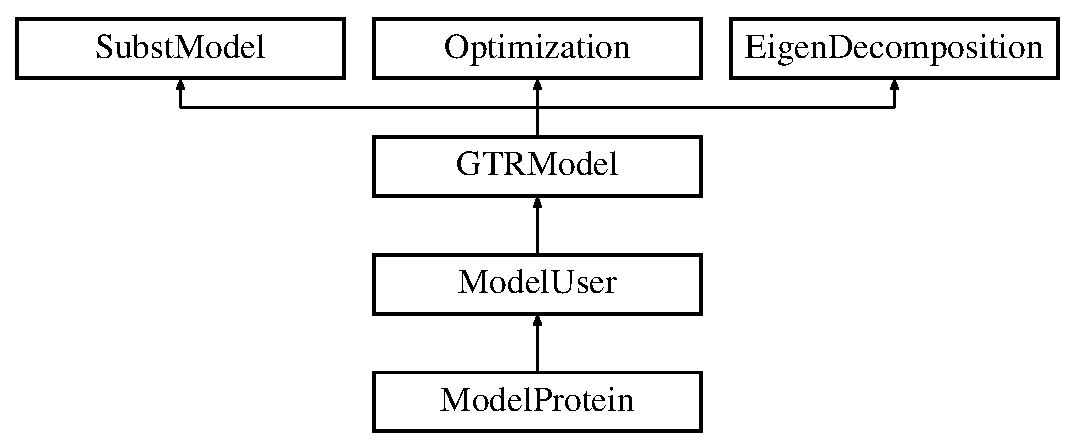
\includegraphics[height=4cm]{classModelProtein}
\end{center}
\end{figure}
\subsection*{Public Member Functions}
\begin{DoxyCompactItemize}
\item 
\hyperlink{classModelProtein_a962861c07a7741cdefb856572fff0757}{ModelProtein} (const char $\ast$model\_\-name, StateFreqType freq, \hyperlink{classPhyloTree}{PhyloTree} $\ast$tree)
\item 
virtual void \hyperlink{classModelProtein_a752778117ce79f5c0161397835fc6bf0}{init} (const char $\ast$model\_\-name, StateFreqType freq)
\item 
virtual void \hyperlink{classModelProtein_a4809c8c2aaa4e5d976214034b3b94df3}{readRates} (istream \&in)  throw (const char$\ast$)
\end{DoxyCompactItemize}


\subsection{Detailed Description}
Substitution models for protein sequences

\begin{DoxyAuthor}{Author}
BUI Quang Minh $<$\href{mailto:minh.bui@univie.ac.at}{\tt minh.bui@univie.ac.at}$>$ 
\end{DoxyAuthor}


\subsection{Constructor \& Destructor Documentation}
\hypertarget{classModelProtein_a962861c07a7741cdefb856572fff0757}{
\index{ModelProtein@{ModelProtein}!ModelProtein@{ModelProtein}}
\index{ModelProtein@{ModelProtein}!ModelProtein@{ModelProtein}}
\subsubsection[{ModelProtein}]{\setlength{\rightskip}{0pt plus 5cm}ModelProtein::ModelProtein (const char $\ast$ {\em model\_\-name}, \/  StateFreqType {\em freq}, \/  {\bf PhyloTree} $\ast$ {\em tree})}}
\label{classModelProtein_a962861c07a7741cdefb856572fff0757}
constructor 
\begin{DoxyParams}{Parameters}
\item[{\em model\_\-name}]model name, e.g., JTT, WAG. \item[{\em freq}]state frequency type \item[{\em tree}]associated phylogenetic tree \end{DoxyParams}


\subsection{Member Function Documentation}
\hypertarget{classModelProtein_a752778117ce79f5c0161397835fc6bf0}{
\index{ModelProtein@{ModelProtein}!init@{init}}
\index{init@{init}!ModelProtein@{ModelProtein}}
\subsubsection[{init}]{\setlength{\rightskip}{0pt plus 5cm}void ModelProtein::init (const char $\ast$ {\em model\_\-name}, \/  StateFreqType {\em freq})\hspace{0.3cm}{\ttfamily  \mbox{[}virtual\mbox{]}}}}
\label{classModelProtein_a752778117ce79f5c0161397835fc6bf0}
initialization, called automatically by the constructor, no need to call it 
\begin{DoxyParams}{Parameters}
\item[{\em model\_\-name}]model name, e.g., JTT, WAG. \item[{\em freq}]state frequency type \end{DoxyParams}


Reimplemented from \hyperlink{classGTRModel_ad0625a75ce5e8f5fca7f65657b2677b8}{GTRModel}.\hypertarget{classModelProtein_a4809c8c2aaa4e5d976214034b3b94df3}{
\index{ModelProtein@{ModelProtein}!readRates@{readRates}}
\index{readRates@{readRates}!ModelProtein@{ModelProtein}}
\subsubsection[{readRates}]{\setlength{\rightskip}{0pt plus 5cm}void ModelProtein::readRates (istream \& {\em in})  throw (const char$\ast$)\hspace{0.3cm}{\ttfamily  \mbox{[}virtual\mbox{]}}}}
\label{classModelProtein_a4809c8c2aaa4e5d976214034b3b94df3}
read the rates from an input stream. it will throw error messages if failed 
\begin{DoxyParams}{Parameters}
\item[{\em in}]input stream \end{DoxyParams}


Reimplemented from \hyperlink{classModelUser_ae0aedeb30d43fbcffcaf5da4bbef5c06}{ModelUser}.

The documentation for this class was generated from the following files:\begin{DoxyCompactItemize}
\item 
src/modelprotein.h\item 
src/modelprotein.cpp\end{DoxyCompactItemize}

\hypertarget{structModelSt}{
\section{ModelSt Struct Reference}
\label{structModelSt}\index{ModelSt@{ModelSt}}
}
\subsection*{Public Attributes}
\begin{DoxyCompactItemize}
\item 
\hypertarget{structModelSt_ae112c8543adfe4b946539d391815856f}{
float {\bfseries ln}}
\label{structModelSt_ae112c8543adfe4b946539d391815856f}

\item 
\hypertarget{structModelSt_af5b410752b63ab6cbf4023a5c6c68d8d}{
int {\bfseries parameters}}
\label{structModelSt_af5b410752b63ab6cbf4023a5c6c68d8d}

\item 
\hypertarget{structModelSt_aaa1ca9eacc333f443da43cd0e26a1ec7}{
char $\ast$ {\bfseries name}}
\label{structModelSt_aaa1ca9eacc333f443da43cd0e26a1ec7}

\end{DoxyCompactItemize}


The documentation for this struct was generated from the following file:\begin{DoxyCompactItemize}
\item 
src/modeltest/modeltest3\_\-7.c\end{DoxyCompactItemize}

\hypertarget{classModelUser}{
\section{ModelUser Class Reference}
\label{classModelUser}\index{ModelUser@{ModelUser}}
}


{\ttfamily \#include $<$modeluser.h$>$}Inheritance diagram for ModelUser::\begin{figure}[H]
\begin{center}
\leavevmode
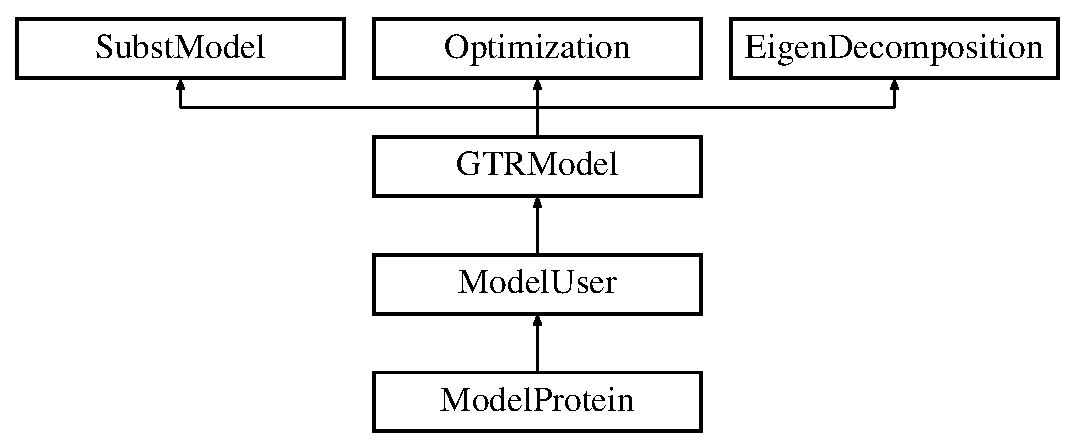
\includegraphics[height=4cm]{classModelUser}
\end{center}
\end{figure}
\subsection*{Public Member Functions}
\begin{DoxyCompactItemize}
\item 
\hyperlink{classModelUser_a69fd20f8460e71c0d2e3f7b0daf015c3}{ModelUser} (\hyperlink{classPhyloTree}{PhyloTree} $\ast$tree)
\item 
virtual void \hyperlink{classModelUser_ae0aedeb30d43fbcffcaf5da4bbef5c06}{readRates} (istream \&in)  throw (const char$\ast$)
\item 
virtual void \hyperlink{classModelUser_a9f0085e7db330321824bf0ccce250bd5}{readStateFreq} (istream \&in)  throw (const char$\ast$)
\item 
virtual int \hyperlink{classModelUser_ad5a88a6c25475b8bb0ea778f4c40cf3b}{getNDim} ()
\end{DoxyCompactItemize}


\subsection{Detailed Description}
User-\/defined models: The rates will be fixed.

\begin{DoxyAuthor}{Author}
BUI Quang Minh $<$\href{mailto:minh.bui@univie.ac.at}{\tt minh.bui@univie.ac.at}$>$ 
\end{DoxyAuthor}


\subsection{Constructor \& Destructor Documentation}
\hypertarget{classModelUser_a69fd20f8460e71c0d2e3f7b0daf015c3}{
\index{ModelUser@{ModelUser}!ModelUser@{ModelUser}}
\index{ModelUser@{ModelUser}!ModelUser@{ModelUser}}
\subsubsection[{ModelUser}]{\setlength{\rightskip}{0pt plus 5cm}ModelUser::ModelUser ({\bf PhyloTree} $\ast$ {\em tree})}}
\label{classModelUser_a69fd20f8460e71c0d2e3f7b0daf015c3}
construction 
\begin{DoxyParams}{Parameters}
\item[{\em tree}]associated phylogenetic tree \end{DoxyParams}


\subsection{Member Function Documentation}
\hypertarget{classModelUser_ad5a88a6c25475b8bb0ea778f4c40cf3b}{
\index{ModelUser@{ModelUser}!getNDim@{getNDim}}
\index{getNDim@{getNDim}!ModelUser@{ModelUser}}
\subsubsection[{getNDim}]{\setlength{\rightskip}{0pt plus 5cm}int ModelUser::getNDim ()\hspace{0.3cm}{\ttfamily  \mbox{[}virtual\mbox{]}}}}
\label{classModelUser_ad5a88a6c25475b8bb0ea778f4c40cf3b}
\begin{DoxyReturn}{Returns}
the number of dimensions 
\end{DoxyReturn}


Reimplemented from \hyperlink{classGTRModel_a6e2066898fbbb245596d4a97dd8ee33c}{GTRModel}.\hypertarget{classModelUser_ae0aedeb30d43fbcffcaf5da4bbef5c06}{
\index{ModelUser@{ModelUser}!readRates@{readRates}}
\index{readRates@{readRates}!ModelUser@{ModelUser}}
\subsubsection[{readRates}]{\setlength{\rightskip}{0pt plus 5cm}void ModelUser::readRates (istream \& {\em in})  throw (const char$\ast$)\hspace{0.3cm}{\ttfamily  \mbox{[}virtual\mbox{]}}}}
\label{classModelUser_ae0aedeb30d43fbcffcaf5da4bbef5c06}
read the rates from an input stream. it will throw error messages if failed 
\begin{DoxyParams}{Parameters}
\item[{\em in}]input stream \end{DoxyParams}


Reimplemented in \hyperlink{classModelProtein_a4809c8c2aaa4e5d976214034b3b94df3}{ModelProtein}.\hypertarget{classModelUser_a9f0085e7db330321824bf0ccce250bd5}{
\index{ModelUser@{ModelUser}!readStateFreq@{readStateFreq}}
\index{readStateFreq@{readStateFreq}!ModelUser@{ModelUser}}
\subsubsection[{readStateFreq}]{\setlength{\rightskip}{0pt plus 5cm}void ModelUser::readStateFreq (istream \& {\em in})  throw (const char$\ast$)\hspace{0.3cm}{\ttfamily  \mbox{[}virtual\mbox{]}}}}
\label{classModelUser_a9f0085e7db330321824bf0ccce250bd5}
read state frequencies from an input stream. it will throw error messages if failed 
\begin{DoxyParams}{Parameters}
\item[{\em in}]input stream \end{DoxyParams}


The documentation for this class was generated from the following files:\begin{DoxyCompactItemize}
\item 
src/modeluser.h\item 
src/modeluser.cpp\end{DoxyCompactItemize}

\hypertarget{classMPdaBlock}{
\section{MPdaBlock Class Reference}
\label{classMPdaBlock}\index{MPdaBlock@{MPdaBlock}}
}


{\ttfamily \#include $<$mpdablock.h$>$}Inheritance diagram for MPdaBlock::\begin{figure}[H]
\begin{center}
\leavevmode
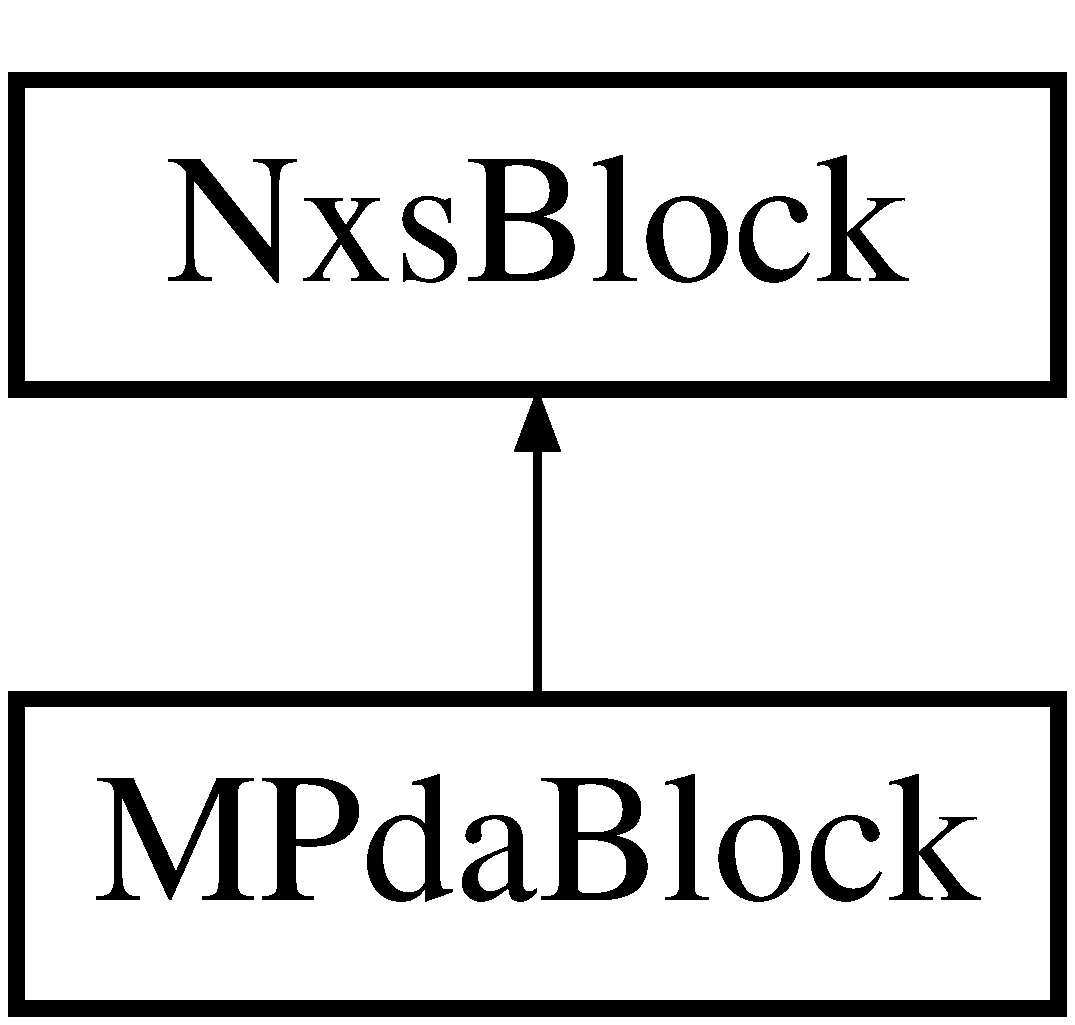
\includegraphics[height=2cm]{classMPdaBlock}
\end{center}
\end{figure}
\subsection*{Public Member Functions}
\begin{DoxyCompactItemize}
\item 
\hyperlink{classMPdaBlock_ae7836b51af1d605dc14372c86b0e996f}{MPdaBlock} (\hyperlink{classSplitGraph}{SplitGraph} $\ast$asgraph)
\item 
virtual \hyperlink{classMPdaBlock_a89cff585f4dcb2f8a2ee1fd6a1c325b0}{$\sim$MPdaBlock} ()
\item 
virtual void \hyperlink{classMPdaBlock_a2ff807bfbacc967eabb5dd643c557fb4}{Report} (ostream \&out)
\item 
virtual void \hyperlink{classMPdaBlock_aba6f6df591c6d1938470e1d13cd9dbef}{Reset} ()
\item 
virtual void \hyperlink{classMPdaBlock_a8fdbc4b20dbfc882e40438a0d8903702}{SkippingCommand} (\hyperlink{classNxsString}{NxsString} commandName)
\item 
void \hyperlink{classMPdaBlock_a0ce085cb000043bf029ef69abf4a97da}{readBudgetFile} (\hyperlink{structParams}{Params} \&params)
\item 
void \hyperlink{classMPdaBlock_af0f2d47828ca74a66567e2655ceb3c83}{readBudgetAreaFile} (\hyperlink{structParams}{Params} \&params)
\item 
int \hyperlink{classMPdaBlock_a670ae262a9f283604cdb289a54f3abd5}{getBudget} ()
\item 
int \hyperlink{classMPdaBlock_a6a41191883550a8b986a2a6e43617ca5}{getMinBudget} ()
\item 
int \hyperlink{classMPdaBlock_a551b1f35390ddf325216d2a70f8adb3f}{getSubSize} ()
\item 
int \hyperlink{classMPdaBlock_a1055777b11e0944b8ca18935f3af6f2e}{getCost} (int tax\_\-id)
\end{DoxyCompactItemize}
\subsection*{Protected Member Functions}
\begin{DoxyCompactItemize}
\item 
virtual void \hyperlink{classMPdaBlock_a80e0ffd8121c77ad6ee49810cd58b1bf}{Read} (\hyperlink{classNxsToken}{NxsToken} \&token)
\end{DoxyCompactItemize}
\subsection*{Protected Attributes}
\begin{DoxyCompactItemize}
\item 
\hyperlink{classSplitGraph}{SplitGraph} $\ast$ \hyperlink{classMPdaBlock_a277cd105fdf1b93184da7deb04279cbb}{sgraph}
\item 
int \hyperlink{classMPdaBlock_a694b0dff038fbd8758c08bfef30adfe5}{budget}
\item 
int \hyperlink{classMPdaBlock_a00091599a4c464c6b530b888bbefc7fd}{min\_\-budget}
\item 
int \hyperlink{classMPdaBlock_a3a6d616fef6b8dfc9f16e098545c5675}{sub\_\-size}
\item 
bool \hyperlink{classMPdaBlock_ab7786c1edc907720b5f309365d6ea070}{cost\_\-constrained}
\item 
vector$<$ int $>$ \hyperlink{classMPdaBlock_a541fd9f72745ea8c285cf1ea8aeb6074}{costs}
\end{DoxyCompactItemize}
\subsection*{Friends}
\begin{DoxyCompactItemize}
\item 
\hypertarget{classMPdaBlock_ab8ea3e9164803ba3b6b59fab949bd0f3}{
class \hyperlink{classMPdaBlock_ab8ea3e9164803ba3b6b59fab949bd0f3}{SplitGraph}}
\label{classMPdaBlock_ab8ea3e9164803ba3b6b59fab949bd0f3}

\item 
\hypertarget{classMPdaBlock_aa341ce7452c8af86ea325aa7eff2f02d}{
class \hyperlink{classMPdaBlock_aa341ce7452c8af86ea325aa7eff2f02d}{PDNetwork}}
\label{classMPdaBlock_aa341ce7452c8af86ea325aa7eff2f02d}

\item 
\hypertarget{classMPdaBlock_a1615e6a0c22088bac5824899e6c3fa6e}{
class \hyperlink{classMPdaBlock_a1615e6a0c22088bac5824899e6c3fa6e}{CircularNetwork}}
\label{classMPdaBlock_a1615e6a0c22088bac5824899e6c3fa6e}

\end{DoxyCompactItemize}


\subsection{Detailed Description}
PdaBlock to read from nexus file

\begin{DoxyAuthor}{Author}
BUI Quang Minh, Steffen Klaere, Arndt von Haeseler 
\end{DoxyAuthor}


\subsection{Constructor \& Destructor Documentation}
\hypertarget{classMPdaBlock_ae7836b51af1d605dc14372c86b0e996f}{
\index{MPdaBlock@{MPdaBlock}!MPdaBlock@{MPdaBlock}}
\index{MPdaBlock@{MPdaBlock}!MPdaBlock@{MPdaBlock}}
\subsubsection[{MPdaBlock}]{\setlength{\rightskip}{0pt plus 5cm}MPdaBlock::MPdaBlock ({\bf SplitGraph} $\ast$ {\em asgraph})}}
\label{classMPdaBlock_ae7836b51af1d605dc14372c86b0e996f}
constructor, assigning an associated splits graph 
\begin{DoxyParams}{Parameters}
\item[{\em asgraph}]a splits graph \end{DoxyParams}
\hypertarget{classMPdaBlock_a89cff585f4dcb2f8a2ee1fd6a1c325b0}{
\index{MPdaBlock@{MPdaBlock}!$\sim$MPdaBlock@{$\sim$MPdaBlock}}
\index{$\sim$MPdaBlock@{$\sim$MPdaBlock}!MPdaBlock@{MPdaBlock}}
\subsubsection[{$\sim$MPdaBlock}]{\setlength{\rightskip}{0pt plus 5cm}MPdaBlock::$\sim$MPdaBlock ()\hspace{0.3cm}{\ttfamily  \mbox{[}virtual\mbox{]}}}}
\label{classMPdaBlock_a89cff585f4dcb2f8a2ee1fd6a1c325b0}
destructor 

\subsection{Member Function Documentation}
\hypertarget{classMPdaBlock_a670ae262a9f283604cdb289a54f3abd5}{
\index{MPdaBlock@{MPdaBlock}!getBudget@{getBudget}}
\index{getBudget@{getBudget}!MPdaBlock@{MPdaBlock}}
\subsubsection[{getBudget}]{\setlength{\rightskip}{0pt plus 5cm}int MPdaBlock::getBudget ()\hspace{0.3cm}{\ttfamily  \mbox{[}inline\mbox{]}}}}
\label{classMPdaBlock_a670ae262a9f283604cdb289a54f3abd5}
\begin{DoxyReturn}{Returns}
total budget 
\end{DoxyReturn}
\hypertarget{classMPdaBlock_a1055777b11e0944b8ca18935f3af6f2e}{
\index{MPdaBlock@{MPdaBlock}!getCost@{getCost}}
\index{getCost@{getCost}!MPdaBlock@{MPdaBlock}}
\subsubsection[{getCost}]{\setlength{\rightskip}{0pt plus 5cm}int MPdaBlock::getCost (int {\em tax\_\-id})\hspace{0.3cm}{\ttfamily  \mbox{[}inline\mbox{]}}}}
\label{classMPdaBlock_a1055777b11e0944b8ca18935f3af6f2e}
\begin{DoxyReturn}{Returns}
cost of a taxon 
\end{DoxyReturn}
\hypertarget{classMPdaBlock_a6a41191883550a8b986a2a6e43617ca5}{
\index{MPdaBlock@{MPdaBlock}!getMinBudget@{getMinBudget}}
\index{getMinBudget@{getMinBudget}!MPdaBlock@{MPdaBlock}}
\subsubsection[{getMinBudget}]{\setlength{\rightskip}{0pt plus 5cm}int MPdaBlock::getMinBudget ()\hspace{0.3cm}{\ttfamily  \mbox{[}inline\mbox{]}}}}
\label{classMPdaBlock_a6a41191883550a8b986a2a6e43617ca5}
\begin{DoxyReturn}{Returns}
min budget 
\end{DoxyReturn}
\hypertarget{classMPdaBlock_a551b1f35390ddf325216d2a70f8adb3f}{
\index{MPdaBlock@{MPdaBlock}!getSubSize@{getSubSize}}
\index{getSubSize@{getSubSize}!MPdaBlock@{MPdaBlock}}
\subsubsection[{getSubSize}]{\setlength{\rightskip}{0pt plus 5cm}int MPdaBlock::getSubSize ()\hspace{0.3cm}{\ttfamily  \mbox{[}inline\mbox{]}}}}
\label{classMPdaBlock_a551b1f35390ddf325216d2a70f8adb3f}
\begin{DoxyReturn}{Returns}
size of PD set 
\end{DoxyReturn}
\hypertarget{classMPdaBlock_a80e0ffd8121c77ad6ee49810cd58b1bf}{
\index{MPdaBlock@{MPdaBlock}!Read@{Read}}
\index{Read@{Read}!MPdaBlock@{MPdaBlock}}
\subsubsection[{Read}]{\setlength{\rightskip}{0pt plus 5cm}void MPdaBlock::Read ({\bf NxsToken} \& {\em token})\hspace{0.3cm}{\ttfamily  \mbox{[}protected, virtual\mbox{]}}}}
\label{classMPdaBlock_a80e0ffd8121c77ad6ee49810cd58b1bf}
main method to read block from file 
\begin{DoxyParams}{Parameters}
\item[{\em token}]a token reader \end{DoxyParams}


Reimplemented from \hyperlink{classNxsBlock}{NxsBlock}.\hypertarget{classMPdaBlock_af0f2d47828ca74a66567e2655ceb3c83}{
\index{MPdaBlock@{MPdaBlock}!readBudgetAreaFile@{readBudgetAreaFile}}
\index{readBudgetAreaFile@{readBudgetAreaFile}!MPdaBlock@{MPdaBlock}}
\subsubsection[{readBudgetAreaFile}]{\setlength{\rightskip}{0pt plus 5cm}void MPdaBlock::readBudgetAreaFile ({\bf Params} \& {\em params})}}
\label{classMPdaBlock_af0f2d47828ca74a66567e2655ceb3c83}
read the file containing total budget and area costs informations 
\begin{DoxyParams}{Parameters}
\item[{\em params}]program parameters \end{DoxyParams}
\hypertarget{classMPdaBlock_a0ce085cb000043bf029ef69abf4a97da}{
\index{MPdaBlock@{MPdaBlock}!readBudgetFile@{readBudgetFile}}
\index{readBudgetFile@{readBudgetFile}!MPdaBlock@{MPdaBlock}}
\subsubsection[{readBudgetFile}]{\setlength{\rightskip}{0pt plus 5cm}void MPdaBlock::readBudgetFile ({\bf Params} \& {\em params})}}
\label{classMPdaBlock_a0ce085cb000043bf029ef69abf4a97da}
read the file containing total budget and taxa costs informations 
\begin{DoxyParams}{Parameters}
\item[{\em params}]program parameters \end{DoxyParams}
\hypertarget{classMPdaBlock_a2ff807bfbacc967eabb5dd643c557fb4}{
\index{MPdaBlock@{MPdaBlock}!Report@{Report}}
\index{Report@{Report}!MPdaBlock@{MPdaBlock}}
\subsubsection[{Report}]{\setlength{\rightskip}{0pt plus 5cm}void MPdaBlock::Report (ostream \& {\em out})\hspace{0.3cm}{\ttfamily  \mbox{[}virtual\mbox{]}}}}
\label{classMPdaBlock_a2ff807bfbacc967eabb5dd643c557fb4}
print info to an output stream 
\begin{DoxyParams}{Parameters}
\item[{\em out}]output stream, cout for output to screen \end{DoxyParams}
\hypertarget{classMPdaBlock_aba6f6df591c6d1938470e1d13cd9dbef}{
\index{MPdaBlock@{MPdaBlock}!Reset@{Reset}}
\index{Reset@{Reset}!MPdaBlock@{MPdaBlock}}
\subsubsection[{Reset}]{\setlength{\rightskip}{0pt plus 5cm}void MPdaBlock::Reset ()\hspace{0.3cm}{\ttfamily  \mbox{[}virtual\mbox{]}}}}
\label{classMPdaBlock_aba6f6df591c6d1938470e1d13cd9dbef}
reset the block 

Reimplemented from \hyperlink{classNxsBlock}{NxsBlock}.\hypertarget{classMPdaBlock_a8fdbc4b20dbfc882e40438a0d8903702}{
\index{MPdaBlock@{MPdaBlock}!SkippingCommand@{SkippingCommand}}
\index{SkippingCommand@{SkippingCommand}!MPdaBlock@{MPdaBlock}}
\subsubsection[{SkippingCommand}]{\setlength{\rightskip}{0pt plus 5cm}void MPdaBlock::SkippingCommand ({\bf NxsString} {\em commandName})\hspace{0.3cm}{\ttfamily  \mbox{[}virtual\mbox{]}}}}
\label{classMPdaBlock_a8fdbc4b20dbfc882e40438a0d8903702}
called when some commands are skipped 
\begin{DoxyParams}{Parameters}
\item[{\em commandName}]command name \end{DoxyParams}


Reimplemented from \hyperlink{classNxsBlock}{NxsBlock}.

\subsection{Member Data Documentation}
\hypertarget{classMPdaBlock_a694b0dff038fbd8758c08bfef30adfe5}{
\index{MPdaBlock@{MPdaBlock}!budget@{budget}}
\index{budget@{budget}!MPdaBlock@{MPdaBlock}}
\subsubsection[{budget}]{\setlength{\rightskip}{0pt plus 5cm}int {\bf MPdaBlock::budget}\hspace{0.3cm}{\ttfamily  \mbox{[}protected\mbox{]}}}}
\label{classMPdaBlock_a694b0dff038fbd8758c08bfef30adfe5}
total budget \hypertarget{classMPdaBlock_ab7786c1edc907720b5f309365d6ea070}{
\index{MPdaBlock@{MPdaBlock}!cost\_\-constrained@{cost\_\-constrained}}
\index{cost\_\-constrained@{cost\_\-constrained}!MPdaBlock@{MPdaBlock}}
\subsubsection[{cost\_\-constrained}]{\setlength{\rightskip}{0pt plus 5cm}bool {\bf MPdaBlock::cost\_\-constrained}\hspace{0.3cm}{\ttfamily  \mbox{[}protected\mbox{]}}}}
\label{classMPdaBlock_ab7786c1edc907720b5f309365d6ea070}
true if cost constrained PD problem \hypertarget{classMPdaBlock_a541fd9f72745ea8c285cf1ea8aeb6074}{
\index{MPdaBlock@{MPdaBlock}!costs@{costs}}
\index{costs@{costs}!MPdaBlock@{MPdaBlock}}
\subsubsection[{costs}]{\setlength{\rightskip}{0pt plus 5cm}vector$<$int$>$ {\bf MPdaBlock::costs}\hspace{0.3cm}{\ttfamily  \mbox{[}protected\mbox{]}}}}
\label{classMPdaBlock_a541fd9f72745ea8c285cf1ea8aeb6074}
cost of each taxon \hypertarget{classMPdaBlock_a00091599a4c464c6b530b888bbefc7fd}{
\index{MPdaBlock@{MPdaBlock}!min\_\-budget@{min\_\-budget}}
\index{min\_\-budget@{min\_\-budget}!MPdaBlock@{MPdaBlock}}
\subsubsection[{min\_\-budget}]{\setlength{\rightskip}{0pt plus 5cm}int {\bf MPdaBlock::min\_\-budget}\hspace{0.3cm}{\ttfamily  \mbox{[}protected\mbox{]}}}}
\label{classMPdaBlock_a00091599a4c464c6b530b888bbefc7fd}
min budget, to compute PD sets with preservation costs from min\_\-budget to budget \hypertarget{classMPdaBlock_a277cd105fdf1b93184da7deb04279cbb}{
\index{MPdaBlock@{MPdaBlock}!sgraph@{sgraph}}
\index{sgraph@{sgraph}!MPdaBlock@{MPdaBlock}}
\subsubsection[{sgraph}]{\setlength{\rightskip}{0pt plus 5cm}{\bf SplitGraph}$\ast$ {\bf MPdaBlock::sgraph}\hspace{0.3cm}{\ttfamily  \mbox{[}protected\mbox{]}}}}
\label{classMPdaBlock_a277cd105fdf1b93184da7deb04279cbb}
the associated splits graph \hypertarget{classMPdaBlock_a3a6d616fef6b8dfc9f16e098545c5675}{
\index{MPdaBlock@{MPdaBlock}!sub\_\-size@{sub\_\-size}}
\index{sub\_\-size@{sub\_\-size}!MPdaBlock@{MPdaBlock}}
\subsubsection[{sub\_\-size}]{\setlength{\rightskip}{0pt plus 5cm}int {\bf MPdaBlock::sub\_\-size}\hspace{0.3cm}{\ttfamily  \mbox{[}protected\mbox{]}}}}
\label{classMPdaBlock_a3a6d616fef6b8dfc9f16e098545c5675}
size of PD set 

The documentation for this class was generated from the following files:\begin{DoxyCompactItemize}
\item 
src/mpdablock.h\item 
src/mpdablock.cpp\end{DoxyCompactItemize}

\hypertarget{classMSetsBlock}{
\section{MSetsBlock Class Reference}
\label{classMSetsBlock}\index{MSetsBlock@{MSetsBlock}}
}


{\ttfamily \#include $<$msetsblock.h$>$}Inheritance diagram for MSetsBlock::\begin{figure}[H]
\begin{center}
\leavevmode
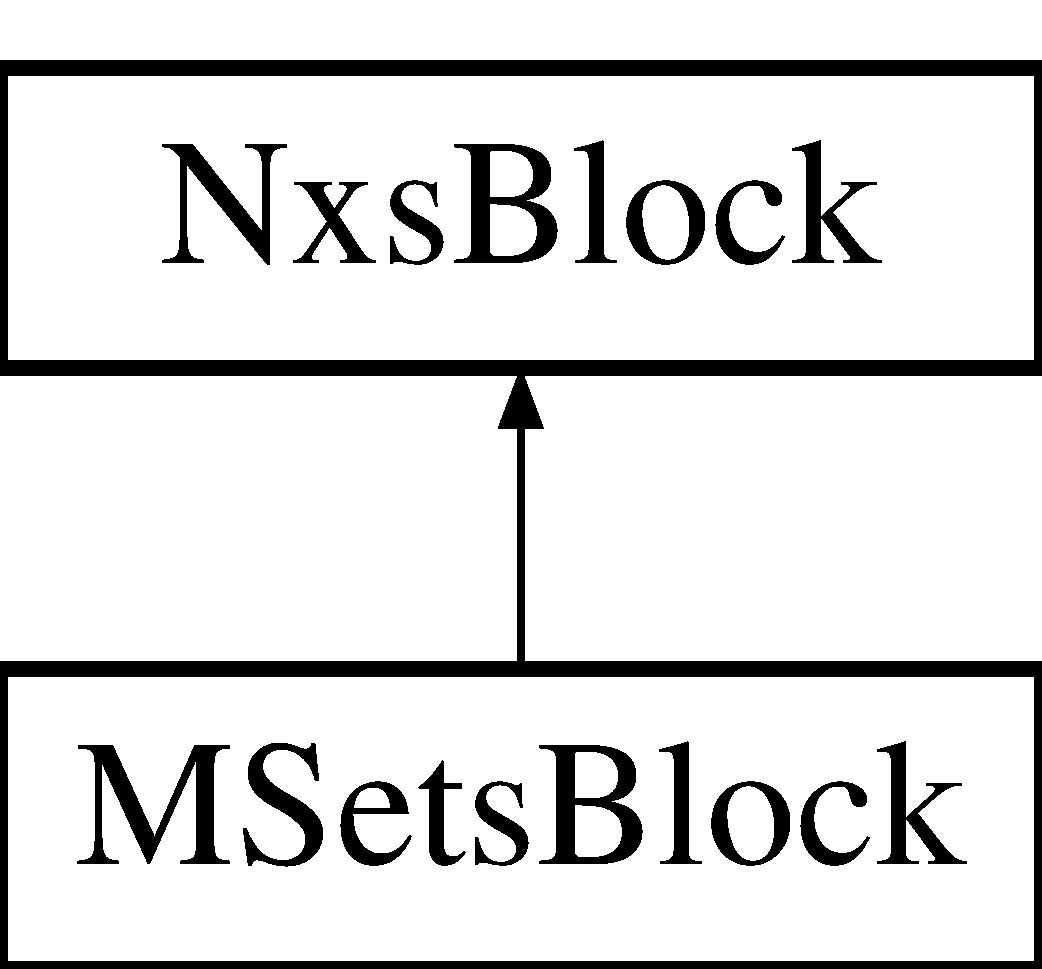
\includegraphics[height=2cm]{classMSetsBlock}
\end{center}
\end{figure}
\subsection*{Public Member Functions}
\begin{DoxyCompactItemize}
\item 
\hyperlink{classMSetsBlock_a46e45cb2258e0c5295d2c22ed8a03333}{MSetsBlock} ()
\item 
virtual \hyperlink{classMSetsBlock_aec8a27486caa13efccfcef0420287c31}{$\sim$MSetsBlock} ()
\item 
virtual void \hyperlink{classMSetsBlock_a88203ea243140fc5402abfecb41ee2c7}{Report} (ostream \&out)
\item 
virtual void \hyperlink{classMSetsBlock_a64e9ca54bba770d1a663de30dfca2073}{Reset} ()
\item 
int \hyperlink{classMSetsBlock_a0950179c8789b05e53fafc981281e694}{getNSets} () const 
\item 
\hyperlink{structTaxaSetName}{TaxaSetName} \& \hyperlink{classMSetsBlock_ac38f25bafc3eaaa704e3bc3d892f3783}{getSet} (int id)
\item 
TaxaSetNameVector \& \hyperlink{classMSetsBlock_af7a44d6b45025b01b20ba612e72c2f4d}{getSets} ()
\item 
int \hyperlink{classMSetsBlock_aae67ce46658428cb5a1793f5ead91ea8}{findArea} (string \&name)
\end{DoxyCompactItemize}
\subsection*{Protected Member Functions}
\begin{DoxyCompactItemize}
\item 
virtual void \hyperlink{classMSetsBlock_ada321520d3bf38ec70c09e8e4568d2fd}{Read} (\hyperlink{classNxsToken}{NxsToken} \&token)
\end{DoxyCompactItemize}
\subsection*{Protected Attributes}
\begin{DoxyCompactItemize}
\item 
TaxaSetNameVector \hyperlink{classMSetsBlock_a30ed727f77895254e40487fc27ae2c97}{sets}
\end{DoxyCompactItemize}


\subsection{Detailed Description}
Sets Block of Nexus file parser

\begin{DoxyAuthor}{Author}
BUI Quang Minh, Steffen Klaere, Arndt von Haeseler 
\end{DoxyAuthor}


\subsection{Constructor \& Destructor Documentation}
\hypertarget{classMSetsBlock_a46e45cb2258e0c5295d2c22ed8a03333}{
\index{MSetsBlock@{MSetsBlock}!MSetsBlock@{MSetsBlock}}
\index{MSetsBlock@{MSetsBlock}!MSetsBlock@{MSetsBlock}}
\subsubsection[{MSetsBlock}]{\setlength{\rightskip}{0pt plus 5cm}MSetsBlock::MSetsBlock ()}}
\label{classMSetsBlock_a46e45cb2258e0c5295d2c22ed8a03333}
constructor, assigning an associated splits graph \hypertarget{classMSetsBlock_aec8a27486caa13efccfcef0420287c31}{
\index{MSetsBlock@{MSetsBlock}!$\sim$MSetsBlock@{$\sim$MSetsBlock}}
\index{$\sim$MSetsBlock@{$\sim$MSetsBlock}!MSetsBlock@{MSetsBlock}}
\subsubsection[{$\sim$MSetsBlock}]{\setlength{\rightskip}{0pt plus 5cm}MSetsBlock::$\sim$MSetsBlock ()\hspace{0.3cm}{\ttfamily  \mbox{[}virtual\mbox{]}}}}
\label{classMSetsBlock_aec8a27486caa13efccfcef0420287c31}
destructor 

\subsection{Member Function Documentation}
\hypertarget{classMSetsBlock_aae67ce46658428cb5a1793f5ead91ea8}{
\index{MSetsBlock@{MSetsBlock}!findArea@{findArea}}
\index{findArea@{findArea}!MSetsBlock@{MSetsBlock}}
\subsubsection[{findArea}]{\setlength{\rightskip}{0pt plus 5cm}int MSetsBlock::findArea (string \& {\em name})}}
\label{classMSetsBlock_aae67ce46658428cb5a1793f5ead91ea8}

\begin{DoxyParams}{Parameters}
\item[{\em name}]an area name \end{DoxyParams}
\begin{DoxyReturn}{Returns}
ID of the area with that name, -\/1 if not found 
\end{DoxyReturn}
\hypertarget{classMSetsBlock_a0950179c8789b05e53fafc981281e694}{
\index{MSetsBlock@{MSetsBlock}!getNSets@{getNSets}}
\index{getNSets@{getNSets}!MSetsBlock@{MSetsBlock}}
\subsubsection[{getNSets}]{\setlength{\rightskip}{0pt plus 5cm}int MSetsBlock::getNSets () const\hspace{0.3cm}{\ttfamily  \mbox{[}inline\mbox{]}}}}
\label{classMSetsBlock_a0950179c8789b05e53fafc981281e694}
\begin{DoxyReturn}{Returns}
the number of sets 
\end{DoxyReturn}
\hypertarget{classMSetsBlock_ac38f25bafc3eaaa704e3bc3d892f3783}{
\index{MSetsBlock@{MSetsBlock}!getSet@{getSet}}
\index{getSet@{getSet}!MSetsBlock@{MSetsBlock}}
\subsubsection[{getSet}]{\setlength{\rightskip}{0pt plus 5cm}{\bf TaxaSetName}\& MSetsBlock::getSet (int {\em id})\hspace{0.3cm}{\ttfamily  \mbox{[}inline\mbox{]}}}}
\label{classMSetsBlock_ac38f25bafc3eaaa704e3bc3d892f3783}

\begin{DoxyParams}{Parameters}
\item[{\em id}]set id \end{DoxyParams}
\begin{DoxyReturn}{Returns}
reference to the corresponding set 
\end{DoxyReturn}
\hypertarget{classMSetsBlock_af7a44d6b45025b01b20ba612e72c2f4d}{
\index{MSetsBlock@{MSetsBlock}!getSets@{getSets}}
\index{getSets@{getSets}!MSetsBlock@{MSetsBlock}}
\subsubsection[{getSets}]{\setlength{\rightskip}{0pt plus 5cm}TaxaSetNameVector\& MSetsBlock::getSets ()\hspace{0.3cm}{\ttfamily  \mbox{[}inline\mbox{]}}}}
\label{classMSetsBlock_af7a44d6b45025b01b20ba612e72c2f4d}
\begin{DoxyReturn}{Returns}
vector of all taxa set 
\end{DoxyReturn}
\hypertarget{classMSetsBlock_ada321520d3bf38ec70c09e8e4568d2fd}{
\index{MSetsBlock@{MSetsBlock}!Read@{Read}}
\index{Read@{Read}!MSetsBlock@{MSetsBlock}}
\subsubsection[{Read}]{\setlength{\rightskip}{0pt plus 5cm}void MSetsBlock::Read ({\bf NxsToken} \& {\em token})\hspace{0.3cm}{\ttfamily  \mbox{[}protected, virtual\mbox{]}}}}
\label{classMSetsBlock_ada321520d3bf38ec70c09e8e4568d2fd}
main method to read block from file 
\begin{DoxyParams}{Parameters}
\item[{\em token}]a token reader \end{DoxyParams}


Reimplemented from \hyperlink{classNxsBlock}{NxsBlock}.\hypertarget{classMSetsBlock_a88203ea243140fc5402abfecb41ee2c7}{
\index{MSetsBlock@{MSetsBlock}!Report@{Report}}
\index{Report@{Report}!MSetsBlock@{MSetsBlock}}
\subsubsection[{Report}]{\setlength{\rightskip}{0pt plus 5cm}void MSetsBlock::Report (ostream \& {\em out})\hspace{0.3cm}{\ttfamily  \mbox{[}virtual\mbox{]}}}}
\label{classMSetsBlock_a88203ea243140fc5402abfecb41ee2c7}
print info to an output stream 
\begin{DoxyParams}{Parameters}
\item[{\em out}]output stream, cout for output to screen \end{DoxyParams}
\hypertarget{classMSetsBlock_a64e9ca54bba770d1a663de30dfca2073}{
\index{MSetsBlock@{MSetsBlock}!Reset@{Reset}}
\index{Reset@{Reset}!MSetsBlock@{MSetsBlock}}
\subsubsection[{Reset}]{\setlength{\rightskip}{0pt plus 5cm}void MSetsBlock::Reset ()\hspace{0.3cm}{\ttfamily  \mbox{[}virtual\mbox{]}}}}
\label{classMSetsBlock_a64e9ca54bba770d1a663de30dfca2073}
reset the block 

Reimplemented from \hyperlink{classNxsBlock}{NxsBlock}.

\subsection{Member Data Documentation}
\hypertarget{classMSetsBlock_a30ed727f77895254e40487fc27ae2c97}{
\index{MSetsBlock@{MSetsBlock}!sets@{sets}}
\index{sets@{sets}!MSetsBlock@{MSetsBlock}}
\subsubsection[{sets}]{\setlength{\rightskip}{0pt plus 5cm}TaxaSetNameVector {\bf MSetsBlock::sets}\hspace{0.3cm}{\ttfamily  \mbox{[}protected\mbox{]}}}}
\label{classMSetsBlock_a30ed727f77895254e40487fc27ae2c97}
list of taxa set names 

The documentation for this class was generated from the following files:\begin{DoxyCompactItemize}
\item 
src/msetsblock.h\item 
src/msetsblock.cpp\end{DoxyCompactItemize}

\hypertarget{classMSplitsBlock}{
\section{MSplitsBlock Class Reference}
\label{classMSplitsBlock}\index{MSplitsBlock@{MSplitsBlock}}
}


{\ttfamily \#include $<$msplitsblock.h$>$}Inheritance diagram for MSplitsBlock::\begin{figure}[H]
\begin{center}
\leavevmode
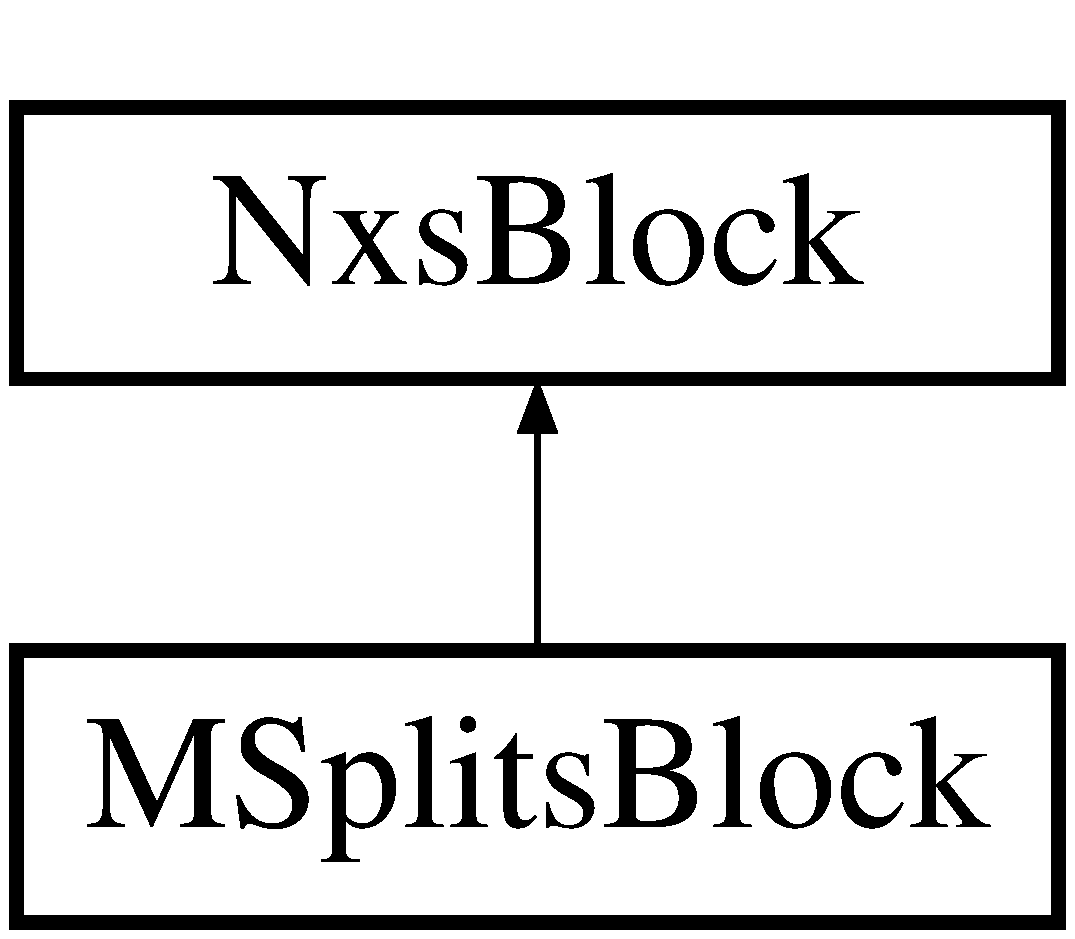
\includegraphics[height=2cm]{classMSplitsBlock}
\end{center}
\end{figure}
\subsection*{Public Member Functions}
\begin{DoxyCompactItemize}
\item 
\hyperlink{classMSplitsBlock_a17ec9ef3354fde89163fd1ee6c22d5d6}{MSplitsBlock} (\hyperlink{classSplitGraph}{SplitGraph} $\ast$asgraph)
\item 
virtual \hyperlink{classMSplitsBlock_a214ec1c6f4a93bafc034d58794e0ca52}{$\sim$MSplitsBlock} ()
\item 
virtual void \hyperlink{classMSplitsBlock_a693bbbb86942e0ede5f21e2aa9caf008}{Report} (ostream \&out)
\item 
virtual void \hyperlink{classMSplitsBlock_ab05dcffb5cbb74d05a809e1ca81d7e23}{Reset} ()
\item 
void \hyperlink{classMSplitsBlock_a3f4b4b3afd38d0ddf0dc553836fd9e73}{AddSplit} (\hyperlink{classNxsToken}{NxsToken} \&token)
\item 
vector$<$ int $>$ \& \hyperlink{classMSplitsBlock_a900cb7fe40906072a3cf490ae647c5ce}{getCycle} ()
\end{DoxyCompactItemize}
\subsection*{Protected Member Functions}
\begin{DoxyCompactItemize}
\item 
virtual void \hyperlink{classMSplitsBlock_a4eb9285aac79a0a29bc0f6be59a4b229}{Read} (\hyperlink{classNxsToken}{NxsToken} \&token)
\end{DoxyCompactItemize}
\subsection*{Protected Attributes}
\begin{DoxyCompactItemize}
\item 
int \hyperlink{classMSplitsBlock_abe567d446c6da8b7f31a3ac1e975cf2b}{ntaxa}
\item 
int \hyperlink{classMSplitsBlock_a6cc2af084a4652277e09c85b2feaea37}{nsplits}
\item 
\hyperlink{classSplitGraph}{SplitGraph} $\ast$ \hyperlink{classMSplitsBlock_a6b5251e50f2faf8c1ae161d2c76ca266}{sgraph}
\item 
vector$<$ int $>$ \hyperlink{classMSplitsBlock_a243b83ab3a6a5c3206da496475765d9d}{cycle}
\end{DoxyCompactItemize}
\subsection*{Friends}
\begin{DoxyCompactItemize}
\item 
\hypertarget{classMSplitsBlock_ab8ea3e9164803ba3b6b59fab949bd0f3}{
class \hyperlink{classMSplitsBlock_ab8ea3e9164803ba3b6b59fab949bd0f3}{SplitGraph}}
\label{classMSplitsBlock_ab8ea3e9164803ba3b6b59fab949bd0f3}

\item 
\hypertarget{classMSplitsBlock_a7a747beac427dfc013c53501e474d452}{
class \hyperlink{classMSplitsBlock_a7a747beac427dfc013c53501e474d452}{MTree}}
\label{classMSplitsBlock_a7a747beac427dfc013c53501e474d452}

\end{DoxyCompactItemize}


\subsection{Detailed Description}
SplitsBlock to read from nexus file

\begin{DoxyAuthor}{Author}
BUI Quang Minh, Steffen Klaere, Arndt von Haeseler 
\end{DoxyAuthor}


\subsection{Constructor \& Destructor Documentation}
\hypertarget{classMSplitsBlock_a17ec9ef3354fde89163fd1ee6c22d5d6}{
\index{MSplitsBlock@{MSplitsBlock}!MSplitsBlock@{MSplitsBlock}}
\index{MSplitsBlock@{MSplitsBlock}!MSplitsBlock@{MSplitsBlock}}
\subsubsection[{MSplitsBlock}]{\setlength{\rightskip}{0pt plus 5cm}MSplitsBlock::MSplitsBlock ({\bf SplitGraph} $\ast$ {\em asgraph})}}
\label{classMSplitsBlock_a17ec9ef3354fde89163fd1ee6c22d5d6}
constructor, assigning an associated splits graph 
\begin{DoxyParams}{Parameters}
\item[{\em asgraph}]a splits graph \end{DoxyParams}
\hypertarget{classMSplitsBlock_a214ec1c6f4a93bafc034d58794e0ca52}{
\index{MSplitsBlock@{MSplitsBlock}!$\sim$MSplitsBlock@{$\sim$MSplitsBlock}}
\index{$\sim$MSplitsBlock@{$\sim$MSplitsBlock}!MSplitsBlock@{MSplitsBlock}}
\subsubsection[{$\sim$MSplitsBlock}]{\setlength{\rightskip}{0pt plus 5cm}MSplitsBlock::$\sim$MSplitsBlock ()\hspace{0.3cm}{\ttfamily  \mbox{[}virtual\mbox{]}}}}
\label{classMSplitsBlock_a214ec1c6f4a93bafc034d58794e0ca52}
destructor 

\subsection{Member Function Documentation}
\hypertarget{classMSplitsBlock_a3f4b4b3afd38d0ddf0dc553836fd9e73}{
\index{MSplitsBlock@{MSplitsBlock}!AddSplit@{AddSplit}}
\index{AddSplit@{AddSplit}!MSplitsBlock@{MSplitsBlock}}
\subsubsection[{AddSplit}]{\setlength{\rightskip}{0pt plus 5cm}void MSplitsBlock::AddSplit ({\bf NxsToken} \& {\em token})}}
\label{classMSplitsBlock_a3f4b4b3afd38d0ddf0dc553836fd9e73}
parse a line containing split 
\begin{DoxyParams}{Parameters}
\item[{\em token}]a token reader \end{DoxyParams}
\hypertarget{classMSplitsBlock_a900cb7fe40906072a3cf490ae647c5ce}{
\index{MSplitsBlock@{MSplitsBlock}!getCycle@{getCycle}}
\index{getCycle@{getCycle}!MSplitsBlock@{MSplitsBlock}}
\subsubsection[{getCycle}]{\setlength{\rightskip}{0pt plus 5cm}vector$<$int$>$\& MSplitsBlock::getCycle ()\hspace{0.3cm}{\ttfamily  \mbox{[}inline\mbox{]}}}}
\label{classMSplitsBlock_a900cb7fe40906072a3cf490ae647c5ce}
\begin{DoxyReturn}{Returns}
cycle 
\end{DoxyReturn}
\hypertarget{classMSplitsBlock_a4eb9285aac79a0a29bc0f6be59a4b229}{
\index{MSplitsBlock@{MSplitsBlock}!Read@{Read}}
\index{Read@{Read}!MSplitsBlock@{MSplitsBlock}}
\subsubsection[{Read}]{\setlength{\rightskip}{0pt plus 5cm}void MSplitsBlock::Read ({\bf NxsToken} \& {\em token})\hspace{0.3cm}{\ttfamily  \mbox{[}protected, virtual\mbox{]}}}}
\label{classMSplitsBlock_a4eb9285aac79a0a29bc0f6be59a4b229}
main method to read block from file 
\begin{DoxyParams}{Parameters}
\item[{\em token}]a token reader \end{DoxyParams}


Reimplemented from \hyperlink{classNxsBlock}{NxsBlock}.\hypertarget{classMSplitsBlock_a693bbbb86942e0ede5f21e2aa9caf008}{
\index{MSplitsBlock@{MSplitsBlock}!Report@{Report}}
\index{Report@{Report}!MSplitsBlock@{MSplitsBlock}}
\subsubsection[{Report}]{\setlength{\rightskip}{0pt plus 5cm}void MSplitsBlock::Report (ostream \& {\em out})\hspace{0.3cm}{\ttfamily  \mbox{[}virtual\mbox{]}}}}
\label{classMSplitsBlock_a693bbbb86942e0ede5f21e2aa9caf008}
print info to an output stream 
\begin{DoxyParams}{Parameters}
\item[{\em out}]output stream, cout for output to screen \end{DoxyParams}
\hypertarget{classMSplitsBlock_ab05dcffb5cbb74d05a809e1ca81d7e23}{
\index{MSplitsBlock@{MSplitsBlock}!Reset@{Reset}}
\index{Reset@{Reset}!MSplitsBlock@{MSplitsBlock}}
\subsubsection[{Reset}]{\setlength{\rightskip}{0pt plus 5cm}void MSplitsBlock::Reset ()\hspace{0.3cm}{\ttfamily  \mbox{[}virtual\mbox{]}}}}
\label{classMSplitsBlock_ab05dcffb5cbb74d05a809e1ca81d7e23}
reset the block 

Reimplemented from \hyperlink{classNxsBlock}{NxsBlock}.

\subsection{Member Data Documentation}
\hypertarget{classMSplitsBlock_a243b83ab3a6a5c3206da496475765d9d}{
\index{MSplitsBlock@{MSplitsBlock}!cycle@{cycle}}
\index{cycle@{cycle}!MSplitsBlock@{MSplitsBlock}}
\subsubsection[{cycle}]{\setlength{\rightskip}{0pt plus 5cm}vector$<$int$>$ {\bf MSplitsBlock::cycle}\hspace{0.3cm}{\ttfamily  \mbox{[}protected\mbox{]}}}}
\label{classMSplitsBlock_a243b83ab3a6a5c3206da496475765d9d}
taxa index around circle, if it is a circular split graph \hypertarget{classMSplitsBlock_a6cc2af084a4652277e09c85b2feaea37}{
\index{MSplitsBlock@{MSplitsBlock}!nsplits@{nsplits}}
\index{nsplits@{nsplits}!MSplitsBlock@{MSplitsBlock}}
\subsubsection[{nsplits}]{\setlength{\rightskip}{0pt plus 5cm}int {\bf MSplitsBlock::nsplits}\hspace{0.3cm}{\ttfamily  \mbox{[}protected\mbox{]}}}}
\label{classMSplitsBlock_a6cc2af084a4652277e09c85b2feaea37}
number of splits \hypertarget{classMSplitsBlock_abe567d446c6da8b7f31a3ac1e975cf2b}{
\index{MSplitsBlock@{MSplitsBlock}!ntaxa@{ntaxa}}
\index{ntaxa@{ntaxa}!MSplitsBlock@{MSplitsBlock}}
\subsubsection[{ntaxa}]{\setlength{\rightskip}{0pt plus 5cm}int {\bf MSplitsBlock::ntaxa}\hspace{0.3cm}{\ttfamily  \mbox{[}protected\mbox{]}}}}
\label{classMSplitsBlock_abe567d446c6da8b7f31a3ac1e975cf2b}
number of taxa \hypertarget{classMSplitsBlock_a6b5251e50f2faf8c1ae161d2c76ca266}{
\index{MSplitsBlock@{MSplitsBlock}!sgraph@{sgraph}}
\index{sgraph@{sgraph}!MSplitsBlock@{MSplitsBlock}}
\subsubsection[{sgraph}]{\setlength{\rightskip}{0pt plus 5cm}{\bf SplitGraph}$\ast$ {\bf MSplitsBlock::sgraph}\hspace{0.3cm}{\ttfamily  \mbox{[}protected\mbox{]}}}}
\label{classMSplitsBlock_a6b5251e50f2faf8c1ae161d2c76ca266}
the associated splits graph 

The documentation for this class was generated from the following files:\begin{DoxyCompactItemize}
\item 
src/msplitsblock.h\item 
src/msplitsblock.cpp\end{DoxyCompactItemize}

\hypertarget{classMTree}{
\section{MTree Class Reference}
\label{classMTree}\index{MTree@{MTree}}
}


{\ttfamily \#include $<$mtree.h$>$}Inheritance diagram for MTree::\begin{figure}[H]
\begin{center}
\leavevmode
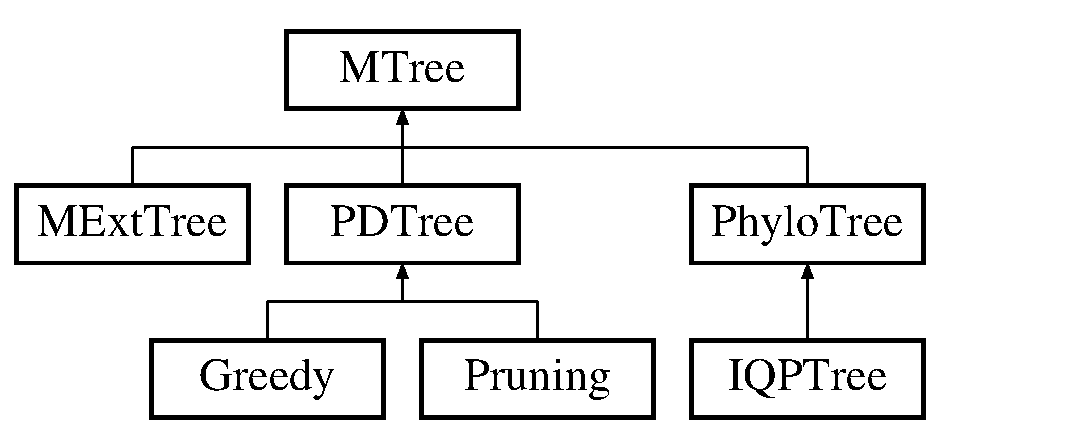
\includegraphics[height=3cm]{classMTree}
\end{center}
\end{figure}
\subsection*{Public Member Functions}
\begin{DoxyCompactItemize}
\item 
\hyperlink{classMTree_ac3f7f958f638616e0728cb8e2b865922}{MTree} (const char $\ast$userTreeFile, bool \&is\_\-rooted)
\item 
\hyperlink{classMTree_aa5d236fb4f1f1fbead1d167675c236c6}{MTree} (\hyperlink{classMTree}{MTree} \&tree)
\item 
\hyperlink{classMTree_aa6a5b154429fee7f9507f8fadce1fe95}{MTree} ()
\item 
virtual void \hyperlink{classMTree_ae1f6543f83abd7236065218131d7ea4b}{copyTree} (\hyperlink{classMTree}{MTree} $\ast$tree)
\item 
void \hyperlink{classMTree_a055e39797764c95c56dadd039eb4d00e}{init} (const char $\ast$userTreeFile, bool \&is\_\-rooted)
\item 
void \hyperlink{classMTree_ad7da0ad44a31e8e98262bd7ad0f494ab}{init} (\hyperlink{classMTree}{MTree} \&tree)
\item 
virtual \hyperlink{classMTree_ab56a0aa9ff7ee51f3b2352a0e80ca973}{$\sim$MTree} ()
\item 
virtual \hyperlink{classNode}{Node} $\ast$ \hyperlink{classMTree_a5e9560ad6b544027bea362387eb2ec3f}{newNode} (int node\_\-id=-\/1, const char $\ast$node\_\-name=NULL)
\item 
\hypertarget{classMTree_a8f1151b6e6d42903b7d02084c8deee43}{
virtual \hyperlink{classNode}{Node} $\ast$ {\bfseries newNode} (int node\_\-id, int node\_\-name)}
\label{classMTree_a8f1151b6e6d42903b7d02084c8deee43}

\item 
void \hyperlink{classMTree_ac186b9f3438e277d476f51803f2d3ce3}{printInfo} (\hyperlink{classNode}{Node} $\ast$node=NULL, \hyperlink{classNode}{Node} $\ast$dad=NULL)
\item 
void \hyperlink{classMTree_a96831ce48d235543e2c5ecb5fed65f75}{printTree} (const char $\ast$outfile, int brtype=WT\_\-BR\_\-LEN)
\item 
void \hyperlink{classMTree_a55093d54d06d5e8841799a9bf7a0ce87}{printTree} (ostream \&out, int brtype=WT\_\-BR\_\-LEN)
\item 
void \hyperlink{classMTree_a822157e8fc26b2d434cc5c1e3129fdf0}{printTree} (ostream \&out, int brtype, \hyperlink{classNode}{Node} $\ast$node, \hyperlink{classNode}{Node} $\ast$dad=NULL)
\item 
void \hyperlink{classMTree_ac360bb6736a82da78866093e3a58123d}{printSubTree} (ostream \&out, NodeVector \&subtree)
\item 
void \hyperlink{classMTree_a898930e7052de462eac23705647762d8}{printSubTree} (ostream \&out, NodeVector \&subtree, \hyperlink{classNode}{Node} $\ast$node, \hyperlink{classNode}{Node} $\ast$dad=NULL)
\item 
void \hyperlink{classMTree_a5d39b487a997d5f5792c19fdc2db0dbe}{printTaxa} (const char $\ast$outfile)
\item 
void \hyperlink{classMTree_a192b058b88470afc75cc588d8c6ebf3d}{printTaxa} (ostream \&out, \hyperlink{classNode}{Node} $\ast$node=NULL, \hyperlink{classNode}{Node} $\ast$dad=NULL)
\item 
void \hyperlink{classMTree_a4c243dff35cd7214acd606ebd59f6bf4}{printTaxa} (ostream \&out, NodeVector \&subtree)
\item 
void \hyperlink{classMTree_abc9c58ea59b80013b0581fe3644c9149}{readTree} (const char $\ast$infile, bool \&is\_\-rooted)
\item 
void \hyperlink{classMTree_a7ca6e031f4df4f38bad9f45a5d4891fb}{readTree} (istream \&in, bool \&is\_\-rooted)
\item 
void \hyperlink{classMTree_a6fa426401166681959012177d0e66f39}{parseFile} (istream \&infile, char \&ch, \hyperlink{classNode}{Node} $\ast$\&\hyperlink{classMTree_af29314a803a9e49bdddd4f5e374bd35e}{root}, double \&branch\_\-len)
\item 
void \hyperlink{classMTree_ad856b7db2e4871e455e1e69c4d5767ae}{initializeTree} (\hyperlink{classNode}{Node} $\ast$node=NULL, \hyperlink{classNode}{Node} $\ast$dad=NULL)
\item 
double \hyperlink{classMTree_a82b21a2f17affae4922b690ea6d2837b}{treeLength} (\hyperlink{classNode}{Node} $\ast$node=NULL, \hyperlink{classNode}{Node} $\ast$dad=NULL)
\item 
void \hyperlink{classMTree_ab0f71f4d94294490f3afe53873d394b5}{getTaxaID} (vector$<$ int $>$ \&taxa, \hyperlink{classNode}{Node} $\ast$node=NULL, \hyperlink{classNode}{Node} $\ast$dad=NULL)
\item 
void \hyperlink{classMTree_af8a50c7ddd8edaf62e10c14e719c6b05}{getTaxa} (NodeVector \&taxa, \hyperlink{classNode}{Node} $\ast$node=NULL, \hyperlink{classNode}{Node} $\ast$dad=NULL)
\item 
void \hyperlink{classMTree_a7552f9cfb570e529ba25a4d6f223ea16}{getTaxaName} (vector$<$ \hyperlink{classNxsString}{NxsString} $>$ \&taxname, \hyperlink{classNode}{Node} $\ast$node=NULL, \hyperlink{classNode}{Node} $\ast$dad=NULL)
\item 
void \hyperlink{classMTree_a26dd819152fe104a747b279619c0e844}{getInternalNodes} (NodeVector \&nodes, \hyperlink{classNode}{Node} $\ast$node=NULL, \hyperlink{classNode}{Node} $\ast$dad=NULL)
\item 
\hyperlink{classNode}{Node} $\ast$ \hyperlink{classMTree_a9bccf760c31c8eb021c4c93eb40575ed}{findNodeName} (string \&name, \hyperlink{classNode}{Node} $\ast$node=NULL, \hyperlink{classNode}{Node} $\ast$dad=NULL)
\item 
\hyperlink{classNode}{Node} $\ast$ \hyperlink{classMTree_a391cb6c0dc914177caa89a42a5fb8dcc}{findNodeID} (int id, \hyperlink{classNode}{Node} $\ast$node=NULL, \hyperlink{classNode}{Node} $\ast$dad=NULL)
\item 
void \hyperlink{classMTree_a2f178b012e999e855bafa053a8caba8f}{scaleLength} (double norm, bool make\_\-int=false, \hyperlink{classNode}{Node} $\ast$node=NULL, \hyperlink{classNode}{Node} $\ast$dad=NULL)
\item 
void \hyperlink{classMTree_a3d183600999c6af85817be3959b43ca8}{scaleCladeSupport} (double norm, bool make\_\-int=false, \hyperlink{classNode}{Node} $\ast$node=NULL, \hyperlink{classNode}{Node} $\ast$dad=NULL)
\item 
void \hyperlink{classMTree_a95c626b2d8172ad06fabab353a77346e}{convertSplits} (\hyperlink{classSplitGraph}{SplitGraph} \&sg)
\item 
void \hyperlink{classMTree_a491979300fde5d4fac2f820c6ae327af}{convertSplits} (vector$<$ \hyperlink{classNxsString}{NxsString} $>$ \&taxname, \hyperlink{classSplitGraph}{SplitGraph} \&sg)
\item 
void \hyperlink{classMTree_a4f9af679d8d53b11044343f6a394e9ab}{convertSplits} (\hyperlink{classSplitGraph}{SplitGraph} \&sg, \hyperlink{classSplit}{Split} $\ast$resp, \hyperlink{classNode}{Node} $\ast$node=NULL, \hyperlink{classNode}{Node} $\ast$dad=NULL)
\item 
void \hyperlink{classMTree_abd4b8cde5e2244eac599a42b33f21698}{convertToTree} (\hyperlink{classSplitGraph}{SplitGraph} \&sg)
\end{DoxyCompactItemize}
\subsection*{Public Attributes}
\begin{DoxyCompactItemize}
\item 
\hyperlink{classNode}{Node} $\ast$ \hyperlink{classMTree_af29314a803a9e49bdddd4f5e374bd35e}{root}
\item 
int \hyperlink{classMTree_a8fe3d41dd96bf4507c60f2c73dcb1026}{leafNum}
\item 
int \hyperlink{classMTree_a1b8904ca0e0218081a92233cbe21478c}{nodeNum}
\item 
bool \hyperlink{classMTree_ae9131924ff162d9cda80333b6f6242b4}{rooted}
\end{DoxyCompactItemize}
\subsection*{Protected Member Functions}
\begin{DoxyCompactItemize}
\item 
void \hyperlink{classMTree_ad81304aa2535e3e43f28eadcb5471c07}{freeNode} (\hyperlink{classNode}{Node} $\ast$node=NULL, \hyperlink{classNode}{Node} $\ast$dad=NULL)
\item 
void \hyperlink{classMTree_a4ba0e04e2f9a71b98eb2c640a1931fa7}{checkValidTree} (bool \&stop, \hyperlink{classNode}{Node} $\ast$node=NULL, \hyperlink{classNode}{Node} $\ast$dad=NULL)
\end{DoxyCompactItemize}


\subsection{Detailed Description}
General-\/purposed tree \begin{DoxyAuthor}{Author}
BUI Quang Minh, Steffen Klaere, Arndt von Haeseler 
\end{DoxyAuthor}


\subsection{Constructor \& Destructor Documentation}
\hypertarget{classMTree_ac3f7f958f638616e0728cb8e2b865922}{
\index{MTree@{MTree}!MTree@{MTree}}
\index{MTree@{MTree}!MTree@{MTree}}
\subsubsection[{MTree}]{\setlength{\rightskip}{0pt plus 5cm}MTree::MTree (const char $\ast$ {\em userTreeFile}, \/  bool \& {\em is\_\-rooted})}}
\label{classMTree_ac3f7f958f638616e0728cb8e2b865922}
constructor, read tree from user file 
\begin{DoxyParams}{Parameters}
\item[{\em userTreeFile}]the name of the user tree \item[{\em is\_\-rooted}](IN/OUT) true if tree is rooted \end{DoxyParams}
\hypertarget{classMTree_aa5d236fb4f1f1fbead1d167675c236c6}{
\index{MTree@{MTree}!MTree@{MTree}}
\index{MTree@{MTree}!MTree@{MTree}}
\subsubsection[{MTree}]{\setlength{\rightskip}{0pt plus 5cm}MTree::MTree ({\bf MTree} \& {\em tree})}}
\label{classMTree_aa5d236fb4f1f1fbead1d167675c236c6}
constructor, get from another tree 
\begin{DoxyParams}{Parameters}
\item[{\em tree}]another \hyperlink{classMTree}{MTree}\end{DoxyParams}
constructor, get from another tree \hypertarget{classMTree_aa6a5b154429fee7f9507f8fadce1fe95}{
\index{MTree@{MTree}!MTree@{MTree}}
\index{MTree@{MTree}!MTree@{MTree}}
\subsubsection[{MTree}]{\setlength{\rightskip}{0pt plus 5cm}MTree::MTree ()}}
\label{classMTree_aa6a5b154429fee7f9507f8fadce1fe95}
constructor \hypertarget{classMTree_ab56a0aa9ff7ee51f3b2352a0e80ca973}{
\index{MTree@{MTree}!$\sim$MTree@{$\sim$MTree}}
\index{$\sim$MTree@{$\sim$MTree}!MTree@{MTree}}
\subsubsection[{$\sim$MTree}]{\setlength{\rightskip}{0pt plus 5cm}MTree::$\sim$MTree ()\hspace{0.3cm}{\ttfamily  \mbox{[}virtual\mbox{]}}}}
\label{classMTree_ab56a0aa9ff7ee51f3b2352a0e80ca973}
destructor 

\subsection{Member Function Documentation}
\hypertarget{classMTree_a4ba0e04e2f9a71b98eb2c640a1931fa7}{
\index{MTree@{MTree}!checkValidTree@{checkValidTree}}
\index{checkValidTree@{checkValidTree}!MTree@{MTree}}
\subsubsection[{checkValidTree}]{\setlength{\rightskip}{0pt plus 5cm}void MTree::checkValidTree (bool \& {\em stop}, \/  {\bf Node} $\ast$ {\em node} = {\ttfamily NULL}, \/  {\bf Node} $\ast$ {\em dad} = {\ttfamily NULL})\hspace{0.3cm}{\ttfamily  \mbox{[}protected\mbox{]}}}}
\label{classMTree_a4ba0e04e2f9a71b98eb2c640a1931fa7}
check tree is bifurcating tree (every leaf with level 1 or 3) 
\begin{DoxyParams}{Parameters}
\item[{\em node}]the starting node, NULL to start from the root \item[{\em dad}]dad of the node, used to direct the search \item[{\em stop}](IN/OUT) set = true to stop the search\end{DoxyParams}
check tree is bifurcating tree (every leaf with level 1 or 3) \hypertarget{classMTree_a4f9af679d8d53b11044343f6a394e9ab}{
\index{MTree@{MTree}!convertSplits@{convertSplits}}
\index{convertSplits@{convertSplits}!MTree@{MTree}}
\subsubsection[{convertSplits}]{\setlength{\rightskip}{0pt plus 5cm}void MTree::convertSplits ({\bf SplitGraph} \& {\em sg}, \/  {\bf Split} $\ast$ {\em resp}, \/  {\bf Node} $\ast$ {\em node} = {\ttfamily NULL}, \/  {\bf Node} $\ast$ {\em dad} = {\ttfamily NULL})}}
\label{classMTree_a4f9af679d8d53b11044343f6a394e9ab}
convert the tree into the split system, iterative procedure 
\begin{DoxyParams}{Parameters}
\item[{\em sg}](OUT) resulting split graph \item[{\em resp}](internal) set of taxa below node \item[{\em node}]the starting node, NULL to start from the root \item[{\em dad}]dad of the node, used to direct the search \end{DoxyParams}
\hypertarget{classMTree_a491979300fde5d4fac2f820c6ae327af}{
\index{MTree@{MTree}!convertSplits@{convertSplits}}
\index{convertSplits@{convertSplits}!MTree@{MTree}}
\subsubsection[{convertSplits}]{\setlength{\rightskip}{0pt plus 5cm}void MTree::convertSplits (vector$<$ {\bf NxsString} $>$ \& {\em taxname}, \/  {\bf SplitGraph} \& {\em sg})}}
\label{classMTree_a491979300fde5d4fac2f820c6ae327af}
convert the tree into the split system 
\begin{DoxyParams}{Parameters}
\item[{\em taxname}]certain taxa name \item[{\em sg}](OUT) resulting split graph \end{DoxyParams}
\hypertarget{classMTree_a95c626b2d8172ad06fabab353a77346e}{
\index{MTree@{MTree}!convertSplits@{convertSplits}}
\index{convertSplits@{convertSplits}!MTree@{MTree}}
\subsubsection[{convertSplits}]{\setlength{\rightskip}{0pt plus 5cm}void MTree::convertSplits ({\bf SplitGraph} \& {\em sg})}}
\label{classMTree_a95c626b2d8172ad06fabab353a77346e}
convert the tree into the split system 
\begin{DoxyParams}{Parameters}
\item[{\em sg}](OUT) resulting split graph \end{DoxyParams}
\hypertarget{classMTree_abd4b8cde5e2244eac599a42b33f21698}{
\index{MTree@{MTree}!convertToTree@{convertToTree}}
\index{convertToTree@{convertToTree}!MTree@{MTree}}
\subsubsection[{convertToTree}]{\setlength{\rightskip}{0pt plus 5cm}void MTree::convertToTree ({\bf SplitGraph} \& {\em sg})}}
\label{classMTree_abd4b8cde5e2244eac599a42b33f21698}
convert compatible split set into tree 
\begin{DoxyParams}{Parameters}
\item[{\em sg}]source split graph \end{DoxyParams}
\hypertarget{classMTree_ae1f6543f83abd7236065218131d7ea4b}{
\index{MTree@{MTree}!copyTree@{copyTree}}
\index{copyTree@{copyTree}!MTree@{MTree}}
\subsubsection[{copyTree}]{\setlength{\rightskip}{0pt plus 5cm}void MTree::copyTree ({\bf MTree} $\ast$ {\em tree})\hspace{0.3cm}{\ttfamily  \mbox{[}virtual\mbox{]}}}}
\label{classMTree_ae1f6543f83abd7236065218131d7ea4b}
copy the tree structure into this tree 
\begin{DoxyParams}{Parameters}
\item[{\em tree}]the tree to copy \end{DoxyParams}
\hypertarget{classMTree_a391cb6c0dc914177caa89a42a5fb8dcc}{
\index{MTree@{MTree}!findNodeID@{findNodeID}}
\index{findNodeID@{findNodeID}!MTree@{MTree}}
\subsubsection[{findNodeID}]{\setlength{\rightskip}{0pt plus 5cm}{\bf Node} $\ast$ MTree::findNodeID (int {\em id}, \/  {\bf Node} $\ast$ {\em node} = {\ttfamily NULL}, \/  {\bf Node} $\ast$ {\em dad} = {\ttfamily NULL})}}
\label{classMTree_a391cb6c0dc914177caa89a42a5fb8dcc}
find a node with corresponding ID 
\begin{DoxyParams}{Parameters}
\item[{\em id}]node ID \item[{\em node}]the starting node, NULL to start from the root \item[{\em dad}]dad of the node, used to direct the search \end{DoxyParams}
\begin{DoxyReturn}{Returns}
node if found, otherwise NULL 
\end{DoxyReturn}
\hypertarget{classMTree_a9bccf760c31c8eb021c4c93eb40575ed}{
\index{MTree@{MTree}!findNodeName@{findNodeName}}
\index{findNodeName@{findNodeName}!MTree@{MTree}}
\subsubsection[{findNodeName}]{\setlength{\rightskip}{0pt plus 5cm}{\bf Node} $\ast$ MTree::findNodeName (string \& {\em name}, \/  {\bf Node} $\ast$ {\em node} = {\ttfamily NULL}, \/  {\bf Node} $\ast$ {\em dad} = {\ttfamily NULL})}}
\label{classMTree_a9bccf760c31c8eb021c4c93eb40575ed}
find a node with corresponding name 
\begin{DoxyParams}{Parameters}
\item[{\em name}]node name \item[{\em node}]the starting node, NULL to start from the root \item[{\em dad}]dad of the node, used to direct the search \end{DoxyParams}
\begin{DoxyReturn}{Returns}
node if found, otherwise NULL 
\end{DoxyReturn}
\hypertarget{classMTree_ad81304aa2535e3e43f28eadcb5471c07}{
\index{MTree@{MTree}!freeNode@{freeNode}}
\index{freeNode@{freeNode}!MTree@{MTree}}
\subsubsection[{freeNode}]{\setlength{\rightskip}{0pt plus 5cm}void MTree::freeNode ({\bf Node} $\ast$ {\em node} = {\ttfamily NULL}, \/  {\bf Node} $\ast$ {\em dad} = {\ttfamily NULL})\hspace{0.3cm}{\ttfamily  \mbox{[}protected\mbox{]}}}}
\label{classMTree_ad81304aa2535e3e43f28eadcb5471c07}
release the nemory. 
\begin{DoxyParams}{Parameters}
\item[{\em node}]the starting node, NULL to start from the root \item[{\em dad}]dad of the node, used to direct the search \end{DoxyParams}
\hypertarget{classMTree_a26dd819152fe104a747b279619c0e844}{
\index{MTree@{MTree}!getInternalNodes@{getInternalNodes}}
\index{getInternalNodes@{getInternalNodes}!MTree@{MTree}}
\subsubsection[{getInternalNodes}]{\setlength{\rightskip}{0pt plus 5cm}void MTree::getInternalNodes (NodeVector \& {\em nodes}, \/  {\bf Node} $\ast$ {\em node} = {\ttfamily NULL}, \/  {\bf Node} $\ast$ {\em dad} = {\ttfamily NULL})}}
\label{classMTree_a26dd819152fe104a747b279619c0e844}
get the descending internal nodes below the node 
\begin{DoxyParams}{Parameters}
\item[{\em node}]the starting node, NULL to start from the root \item[{\em dad}]dad of the node, used to direct the search \item[{\em nodes}](OUT) vector of internal nodes \end{DoxyParams}
\hypertarget{classMTree_af8a50c7ddd8edaf62e10c14e719c6b05}{
\index{MTree@{MTree}!getTaxa@{getTaxa}}
\index{getTaxa@{getTaxa}!MTree@{MTree}}
\subsubsection[{getTaxa}]{\setlength{\rightskip}{0pt plus 5cm}void MTree::getTaxa (NodeVector \& {\em taxa}, \/  {\bf Node} $\ast$ {\em node} = {\ttfamily NULL}, \/  {\bf Node} $\ast$ {\em dad} = {\ttfamily NULL})}}
\label{classMTree_af8a50c7ddd8edaf62e10c14e719c6b05}
get the descending taxa below the node 
\begin{DoxyParams}{Parameters}
\item[{\em node}]the starting node, NULL to start from the root \item[{\em dad}]dad of the node, used to direct the search \item[{\em taxa}](OUT) vector of taxa \end{DoxyParams}
\hypertarget{classMTree_ab0f71f4d94294490f3afe53873d394b5}{
\index{MTree@{MTree}!getTaxaID@{getTaxaID}}
\index{getTaxaID@{getTaxaID}!MTree@{MTree}}
\subsubsection[{getTaxaID}]{\setlength{\rightskip}{0pt plus 5cm}void MTree::getTaxaID (vector$<$ int $>$ \& {\em taxa}, \/  {\bf Node} $\ast$ {\em node} = {\ttfamily NULL}, \/  {\bf Node} $\ast$ {\em dad} = {\ttfamily NULL})}}
\label{classMTree_ab0f71f4d94294490f3afe53873d394b5}
get the descending taxa ID list below the node 
\begin{DoxyParams}{Parameters}
\item[{\em node}]the starting node, NULL to start from the root \item[{\em dad}]dad of the node, used to direct the search \item[{\em taxa}](OUT) taxa ID \end{DoxyParams}
\hypertarget{classMTree_a7552f9cfb570e529ba25a4d6f223ea16}{
\index{MTree@{MTree}!getTaxaName@{getTaxaName}}
\index{getTaxaName@{getTaxaName}!MTree@{MTree}}
\subsubsection[{getTaxaName}]{\setlength{\rightskip}{0pt plus 5cm}void MTree::getTaxaName (vector$<$ {\bf NxsString} $>$ \& {\em taxname}, \/  {\bf Node} $\ast$ {\em node} = {\ttfamily NULL}, \/  {\bf Node} $\ast$ {\em dad} = {\ttfamily NULL})}}
\label{classMTree_a7552f9cfb570e529ba25a4d6f223ea16}
get the descending taxa names below the node 
\begin{DoxyParams}{Parameters}
\item[{\em node}]the starting node, NULL to start from the root \item[{\em dad}]dad of the node, used to direct the search \item[{\em taxname}](OUT) taxa name \end{DoxyParams}
\hypertarget{classMTree_ad7da0ad44a31e8e98262bd7ad0f494ab}{
\index{MTree@{MTree}!init@{init}}
\index{init@{init}!MTree@{MTree}}
\subsubsection[{init}]{\setlength{\rightskip}{0pt plus 5cm}void MTree::init ({\bf MTree} \& {\em tree})}}
\label{classMTree_ad7da0ad44a31e8e98262bd7ad0f494ab}
initialize tree, get from another tree 
\begin{DoxyParams}{Parameters}
\item[{\em tree}]another \hyperlink{classMTree}{MTree} \end{DoxyParams}


Reimplemented in \hyperlink{classPDTree_a423ef933e7940c5c745e27898a394bfc}{PDTree}.\hypertarget{classMTree_a055e39797764c95c56dadd039eb4d00e}{
\index{MTree@{MTree}!init@{init}}
\index{init@{init}!MTree@{MTree}}
\subsubsection[{init}]{\setlength{\rightskip}{0pt plus 5cm}void MTree::init (const char $\ast$ {\em userTreeFile}, \/  bool \& {\em is\_\-rooted})}}
\label{classMTree_a055e39797764c95c56dadd039eb4d00e}
initialize the tree from a NEWICK tree file 
\begin{DoxyParams}{Parameters}
\item[{\em userTreeFile}]the name of the user tree \item[{\em is\_\-rooted}](IN/OUT) true if tree is rooted \end{DoxyParams}
\hypertarget{classMTree_ad856b7db2e4871e455e1e69c4d5767ae}{
\index{MTree@{MTree}!initializeTree@{initializeTree}}
\index{initializeTree@{initializeTree}!MTree@{MTree}}
\subsubsection[{initializeTree}]{\setlength{\rightskip}{0pt plus 5cm}void MTree::initializeTree ({\bf Node} $\ast$ {\em node} = {\ttfamily NULL}, \/  {\bf Node} $\ast$ {\em dad} = {\ttfamily NULL})}}
\label{classMTree_ad856b7db2e4871e455e1e69c4d5767ae}
initialize tree, set node structure 
\begin{DoxyParams}{Parameters}
\item[{\em node}]the starting node, NULL to start from the root \item[{\em dad}]dad of the node, used to direct the search \end{DoxyParams}
\hypertarget{classMTree_a5e9560ad6b544027bea362387eb2ec3f}{
\index{MTree@{MTree}!newNode@{newNode}}
\index{newNode@{newNode}!MTree@{MTree}}
\subsubsection[{newNode}]{\setlength{\rightskip}{0pt plus 5cm}{\bf Node} $\ast$ MTree::newNode (int {\em node\_\-id} = {\ttfamily -\/1}, \/  const char $\ast$ {\em node\_\-name} = {\ttfamily NULL})\hspace{0.3cm}{\ttfamily  \mbox{[}virtual\mbox{]}}}}
\label{classMTree_a5e9560ad6b544027bea362387eb2ec3f}
allocate a new node. Override this if you have an inherited \hyperlink{classNode}{Node} class. 
\begin{DoxyParams}{Parameters}
\item[{\em node\_\-id}]node ID \item[{\em node\_\-name}]node name \end{DoxyParams}
\begin{DoxyReturn}{Returns}
a new node 
\end{DoxyReturn}


Reimplemented in \hyperlink{classPhyloTree_a08daeabbb3fa596916aa48834e0b152d}{PhyloTree}.\hypertarget{classMTree_a6fa426401166681959012177d0e66f39}{
\index{MTree@{MTree}!parseFile@{parseFile}}
\index{parseFile@{parseFile}!MTree@{MTree}}
\subsubsection[{parseFile}]{\setlength{\rightskip}{0pt plus 5cm}void MTree::parseFile (istream \& {\em infile}, \/  char \& {\em ch}, \/  {\bf Node} $\ast$\& {\em root}, \/  double \& {\em branch\_\-len})}}
\label{classMTree_a6fa426401166681959012177d0e66f39}
parse the tree from the input file in newick format 
\begin{DoxyParams}{Parameters}
\item[{\em infile}]the input file \item[{\em ch}](IN/OUT) current char \item[{\em root}](IN/OUT) the root of the (sub)tree \item[{\em branch\_\-len}](OUT) branch length associated to the current root \end{DoxyParams}
\hypertarget{classMTree_ac186b9f3438e277d476f51803f2d3ce3}{
\index{MTree@{MTree}!printInfo@{printInfo}}
\index{printInfo@{printInfo}!MTree@{MTree}}
\subsubsection[{printInfo}]{\setlength{\rightskip}{0pt plus 5cm}void MTree::printInfo ({\bf Node} $\ast$ {\em node} = {\ttfamily NULL}, \/  {\bf Node} $\ast$ {\em dad} = {\ttfamily NULL})}}
\label{classMTree_ac186b9f3438e277d476f51803f2d3ce3}
print information 
\begin{DoxyParams}{Parameters}
\item[{\em node}]the starting node, NULL to start from the root \item[{\em dad}]dad of the node, used to direct the search \end{DoxyParams}
\hypertarget{classMTree_a898930e7052de462eac23705647762d8}{
\index{MTree@{MTree}!printSubTree@{printSubTree}}
\index{printSubTree@{printSubTree}!MTree@{MTree}}
\subsubsection[{printSubTree}]{\setlength{\rightskip}{0pt plus 5cm}void MTree::printSubTree (ostream \& {\em out}, \/  NodeVector \& {\em subtree}, \/  {\bf Node} $\ast$ {\em node}, \/  {\bf Node} $\ast$ {\em dad} = {\ttfamily NULL})}}
\label{classMTree_a898930e7052de462eac23705647762d8}
print the sub-\/tree to the output file in newick format 
\begin{DoxyParams}{Parameters}
\item[{\em out}]the output file. \item[{\em node}]the starting node, NULL to start from the root \item[{\em dad}]dad of the node, used to direct the search \item[{\em subtree}]list of nodes (internal \& external) contained in the new tree \end{DoxyParams}
\hypertarget{classMTree_ac360bb6736a82da78866093e3a58123d}{
\index{MTree@{MTree}!printSubTree@{printSubTree}}
\index{printSubTree@{printSubTree}!MTree@{MTree}}
\subsubsection[{printSubTree}]{\setlength{\rightskip}{0pt plus 5cm}void MTree::printSubTree (ostream \& {\em out}, \/  NodeVector \& {\em subtree})}}
\label{classMTree_ac360bb6736a82da78866093e3a58123d}
print the sub-\/tree to the output file in newick format 
\begin{DoxyParams}{Parameters}
\item[{\em out}]the output file. \item[{\em subtree}]list of nodes (internal \& external) contained in the new tree \end{DoxyParams}
\hypertarget{classMTree_a4c243dff35cd7214acd606ebd59f6bf4}{
\index{MTree@{MTree}!printTaxa@{printTaxa}}
\index{printTaxa@{printTaxa}!MTree@{MTree}}
\subsubsection[{printTaxa}]{\setlength{\rightskip}{0pt plus 5cm}void MTree::printTaxa (ostream \& {\em out}, \/  NodeVector \& {\em subtree})}}
\label{classMTree_a4c243dff35cd7214acd606ebd59f6bf4}
print the taxa set of a given subtree 
\begin{DoxyParams}{Parameters}
\item[{\em out}]the output file. \item[{\em subtree}]the subtree vector \end{DoxyParams}
\hypertarget{classMTree_a192b058b88470afc75cc588d8c6ebf3d}{
\index{MTree@{MTree}!printTaxa@{printTaxa}}
\index{printTaxa@{printTaxa}!MTree@{MTree}}
\subsubsection[{printTaxa}]{\setlength{\rightskip}{0pt plus 5cm}void MTree::printTaxa (ostream \& {\em out}, \/  {\bf Node} $\ast$ {\em node} = {\ttfamily NULL}, \/  {\bf Node} $\ast$ {\em dad} = {\ttfamily NULL})}}
\label{classMTree_a192b058b88470afc75cc588d8c6ebf3d}
print the taxa set to the output file 
\begin{DoxyParams}{Parameters}
\item[{\em out}]the output file. \item[{\em node}]the starting node, NULL to start from the root \item[{\em dad}]dad of the node, used to direct the search \end{DoxyParams}
\hypertarget{classMTree_a5d39b487a997d5f5792c19fdc2db0dbe}{
\index{MTree@{MTree}!printTaxa@{printTaxa}}
\index{printTaxa@{printTaxa}!MTree@{MTree}}
\subsubsection[{printTaxa}]{\setlength{\rightskip}{0pt plus 5cm}void MTree::printTaxa (const char $\ast$ {\em outfile})}}
\label{classMTree_a5d39b487a997d5f5792c19fdc2db0dbe}
print the taxa set to the output file 
\begin{DoxyParams}{Parameters}
\item[{\em outfile}]the output file. \end{DoxyParams}
\hypertarget{classMTree_a822157e8fc26b2d434cc5c1e3129fdf0}{
\index{MTree@{MTree}!printTree@{printTree}}
\index{printTree@{printTree}!MTree@{MTree}}
\subsubsection[{printTree}]{\setlength{\rightskip}{0pt plus 5cm}void MTree::printTree (ostream \& {\em out}, \/  int {\em brtype}, \/  {\bf Node} $\ast$ {\em node}, \/  {\bf Node} $\ast$ {\em dad} = {\ttfamily NULL})}}
\label{classMTree_a822157e8fc26b2d434cc5c1e3129fdf0}
print the tree to the output file in newick format 
\begin{DoxyParams}{Parameters}
\item[{\em out}]the output file. \item[{\em node}]the starting node, NULL to start from the root \item[{\em dad}]dad of the node, used to direct the search \item[{\em brtype}]type of branch to print \end{DoxyParams}
\hypertarget{classMTree_a55093d54d06d5e8841799a9bf7a0ce87}{
\index{MTree@{MTree}!printTree@{printTree}}
\index{printTree@{printTree}!MTree@{MTree}}
\subsubsection[{printTree}]{\setlength{\rightskip}{0pt plus 5cm}void MTree::printTree (ostream \& {\em out}, \/  int {\em brtype} = {\ttfamily WT\_\-BR\_\-LEN})}}
\label{classMTree_a55093d54d06d5e8841799a9bf7a0ce87}
print the tree to the output file in newick format 
\begin{DoxyParams}{Parameters}
\item[{\em out}]the output stream. \item[{\em brtype}]type of branch to print \end{DoxyParams}
\hypertarget{classMTree_a96831ce48d235543e2c5ecb5fed65f75}{
\index{MTree@{MTree}!printTree@{printTree}}
\index{printTree@{printTree}!MTree@{MTree}}
\subsubsection[{printTree}]{\setlength{\rightskip}{0pt plus 5cm}void MTree::printTree (const char $\ast$ {\em outfile}, \/  int {\em brtype} = {\ttfamily WT\_\-BR\_\-LEN})}}
\label{classMTree_a96831ce48d235543e2c5ecb5fed65f75}
print the tree to the output file in newick format 
\begin{DoxyParams}{Parameters}
\item[{\em outfile}]the output file. \item[{\em brtype}]type of branch to print \end{DoxyParams}
\hypertarget{classMTree_a7ca6e031f4df4f38bad9f45a5d4891fb}{
\index{MTree@{MTree}!readTree@{readTree}}
\index{readTree@{readTree}!MTree@{MTree}}
\subsubsection[{readTree}]{\setlength{\rightskip}{0pt plus 5cm}void MTree::readTree (istream \& {\em in}, \/  bool \& {\em is\_\-rooted})}}
\label{classMTree_a7ca6e031f4df4f38bad9f45a5d4891fb}
read the tree from the ifstream in newick format 
\begin{DoxyParams}{Parameters}
\item[{\em in}]the input stream. \item[{\em is\_\-rooted}](IN/OUT) true if tree is rooted \end{DoxyParams}
\hypertarget{classMTree_abc9c58ea59b80013b0581fe3644c9149}{
\index{MTree@{MTree}!readTree@{readTree}}
\index{readTree@{readTree}!MTree@{MTree}}
\subsubsection[{readTree}]{\setlength{\rightskip}{0pt plus 5cm}void MTree::readTree (const char $\ast$ {\em infile}, \/  bool \& {\em is\_\-rooted})}}
\label{classMTree_abc9c58ea59b80013b0581fe3644c9149}
read the tree from the input file in newick format 
\begin{DoxyParams}{Parameters}
\item[{\em infile}]the input file file. \item[{\em is\_\-rooted}](IN/OUT) true if tree is rooted \end{DoxyParams}
\hypertarget{classMTree_a3d183600999c6af85817be3959b43ca8}{
\index{MTree@{MTree}!scaleCladeSupport@{scaleCladeSupport}}
\index{scaleCladeSupport@{scaleCladeSupport}!MTree@{MTree}}
\subsubsection[{scaleCladeSupport}]{\setlength{\rightskip}{0pt plus 5cm}void MTree::scaleCladeSupport (double {\em norm}, \/  bool {\em make\_\-int} = {\ttfamily false}, \/  {\bf Node} $\ast$ {\em node} = {\ttfamily NULL}, \/  {\bf Node} $\ast$ {\em dad} = {\ttfamily NULL})}}
\label{classMTree_a3d183600999c6af85817be3959b43ca8}
scale the clade supports of all internal nodes to a norm factor 
\begin{DoxyParams}{Parameters}
\item[{\em norm}]normalized factor \item[{\em make\_\-int}]TRUE to round lengths to int, FALSE otherwise \item[{\em node}]the starting node, NULL to start from the root \item[{\em dad}]dad of the node, used to direct the search \end{DoxyParams}
\hypertarget{classMTree_a2f178b012e999e855bafa053a8caba8f}{
\index{MTree@{MTree}!scaleLength@{scaleLength}}
\index{scaleLength@{scaleLength}!MTree@{MTree}}
\subsubsection[{scaleLength}]{\setlength{\rightskip}{0pt plus 5cm}void MTree::scaleLength (double {\em norm}, \/  bool {\em make\_\-int} = {\ttfamily false}, \/  {\bf Node} $\ast$ {\em node} = {\ttfamily NULL}, \/  {\bf Node} $\ast$ {\em dad} = {\ttfamily NULL})}}
\label{classMTree_a2f178b012e999e855bafa053a8caba8f}
scale the length of all branches to a norm factor 
\begin{DoxyParams}{Parameters}
\item[{\em norm}]normalized factor \item[{\em make\_\-int}]TRUE to round lengths to int, FALSE otherwise \item[{\em node}]the starting node, NULL to start from the root \item[{\em dad}]dad of the node, used to direct the search \end{DoxyParams}
\hypertarget{classMTree_a82b21a2f17affae4922b690ea6d2837b}{
\index{MTree@{MTree}!treeLength@{treeLength}}
\index{treeLength@{treeLength}!MTree@{MTree}}
\subsubsection[{treeLength}]{\setlength{\rightskip}{0pt plus 5cm}double MTree::treeLength ({\bf Node} $\ast$ {\em node} = {\ttfamily NULL}, \/  {\bf Node} $\ast$ {\em dad} = {\ttfamily NULL})}}
\label{classMTree_a82b21a2f17affae4922b690ea6d2837b}
\begin{DoxyReturn}{Returns}
sum of all branch lengths 
\end{DoxyReturn}

\begin{DoxyParams}{Parameters}
\item[{\em node}]the starting node, NULL to start from the root \item[{\em dad}]dad of the node, used to direct the search \end{DoxyParams}


\subsection{Member Data Documentation}
\hypertarget{classMTree_a8fe3d41dd96bf4507c60f2c73dcb1026}{
\index{MTree@{MTree}!leafNum@{leafNum}}
\index{leafNum@{leafNum}!MTree@{MTree}}
\subsubsection[{leafNum}]{\setlength{\rightskip}{0pt plus 5cm}int {\bf MTree::leafNum}}}
\label{classMTree_a8fe3d41dd96bf4507c60f2c73dcb1026}
number of leaves \hypertarget{classMTree_a1b8904ca0e0218081a92233cbe21478c}{
\index{MTree@{MTree}!nodeNum@{nodeNum}}
\index{nodeNum@{nodeNum}!MTree@{MTree}}
\subsubsection[{nodeNum}]{\setlength{\rightskip}{0pt plus 5cm}int {\bf MTree::nodeNum}}}
\label{classMTree_a1b8904ca0e0218081a92233cbe21478c}
total number of nodes in the tree \hypertarget{classMTree_af29314a803a9e49bdddd4f5e374bd35e}{
\index{MTree@{MTree}!root@{root}}
\index{root@{root}!MTree@{MTree}}
\subsubsection[{root}]{\setlength{\rightskip}{0pt plus 5cm}{\bf Node}$\ast$ {\bf MTree::root}}}
\label{classMTree_af29314a803a9e49bdddd4f5e374bd35e}
root node. \hypertarget{classMTree_ae9131924ff162d9cda80333b6f6242b4}{
\index{MTree@{MTree}!rooted@{rooted}}
\index{rooted@{rooted}!MTree@{MTree}}
\subsubsection[{rooted}]{\setlength{\rightskip}{0pt plus 5cm}bool {\bf MTree::rooted}}}
\label{classMTree_ae9131924ff162d9cda80333b6f6242b4}
user tree file name TRUE if the tree is rooted 

The documentation for this class was generated from the following files:\begin{DoxyCompactItemize}
\item 
src/mtree.h\item 
src/mtree.cpp\end{DoxyCompactItemize}

\hypertarget{classMTreeSet}{
\section{MTreeSet Class Reference}
\label{classMTreeSet}\index{MTreeSet@{MTreeSet}}
}


{\ttfamily \#include $<$mtreeset.h$>$}Inheritance diagram for MTreeSet::\begin{figure}[H]
\begin{center}
\leavevmode
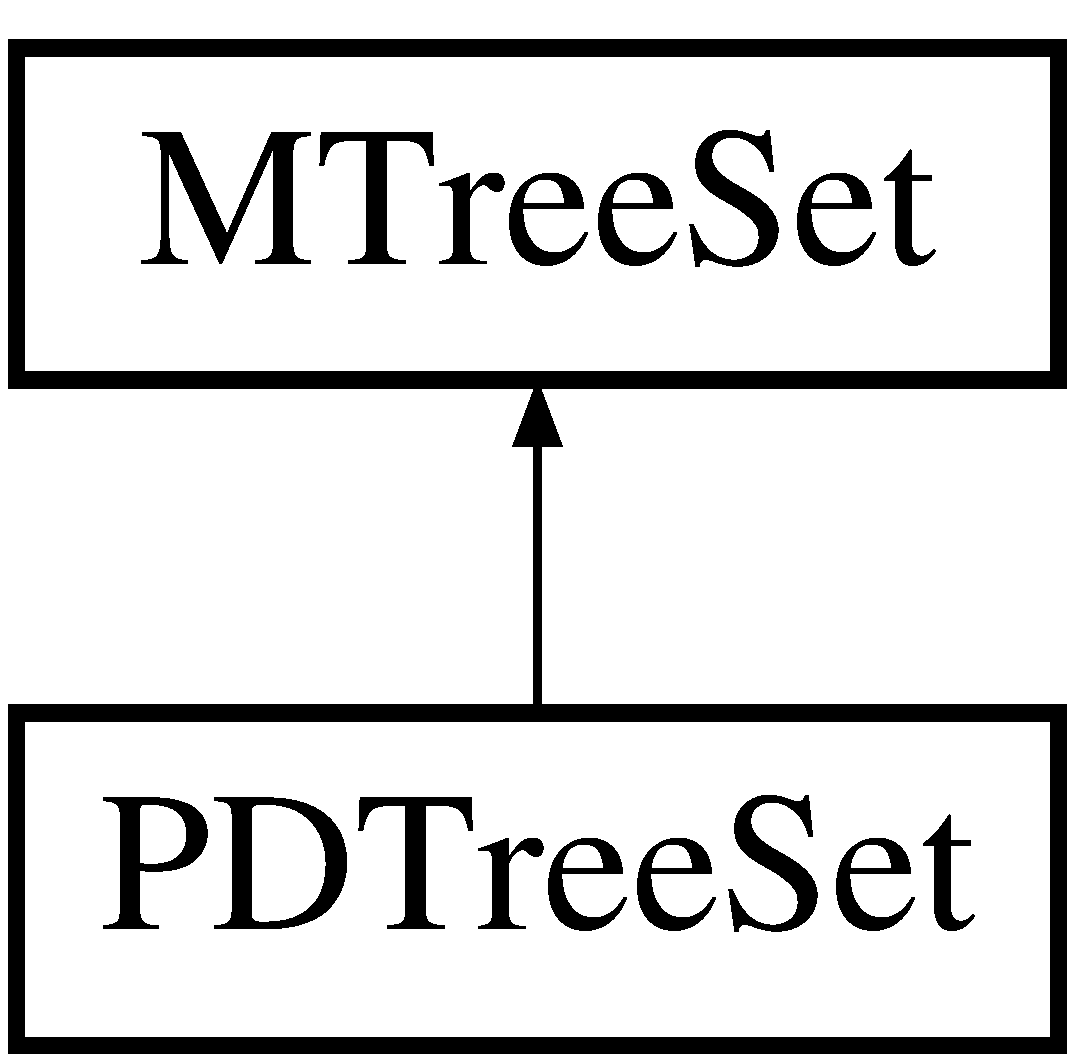
\includegraphics[height=2cm]{classMTreeSet}
\end{center}
\end{figure}
\subsection*{Public Member Functions}
\begin{DoxyCompactItemize}
\item 
\hyperlink{classMTreeSet_a88d94d529da4f81c2fe4537baa794333}{MTreeSet} (const char $\ast$userTreeFile, bool \&is\_\-rooted, int burnin)
\item 
void \hyperlink{classMTreeSet_aef18c58d44d7f2fe2a9cf81e68e570cd}{init} (const char $\ast$userTreeFile, bool \&is\_\-rooted, int burnin)
\item 
void \hyperlink{classMTreeSet_a5522394de84eee1544e021d1baed3655}{readTrees} (const char $\ast$userTreeFile, bool \&is\_\-rooted, int burnin)
\item 
void \hyperlink{classMTreeSet_a0ebff75dc397363dc55622ad094c4432}{checkConsistency} ()
\item 
bool \hyperlink{classMTreeSet_a1788a15758d1c5292f05afb3b7920fbe}{isRooted} ()
\item 
void \hyperlink{classMTreeSet_a0fbde69391914ed669cd05007946867d}{printTrees} (const char $\ast$outfile, int brtype=WT\_\-BR\_\-LEN)
\item 
void \hyperlink{classMTreeSet_ad4401d1bde1649b95439953c218ca224}{printTrees} (ostream \&out, int brtype=WT\_\-BR\_\-LEN)
\item 
void \hyperlink{classMTreeSet_ae937b8a9957d096c14b2fa9364c6c660}{convertSplits} (vector$<$ \hyperlink{classNxsString}{NxsString} $>$ \&taxname, \hyperlink{classSplitGraph}{SplitGraph} \&sg, \hyperlink{classSplitIntMap}{SplitIntMap} \&hash\_\-ss, bool lensum)
\item 
void \hyperlink{classMTreeSet_ae973cf95e914256097ee21fd2491b89a}{convertSplits} (\hyperlink{classSplitGraph}{SplitGraph} \&sg, \hyperlink{classSplitIntMap}{SplitIntMap} \&hash\_\-ss, bool lensum)
\item 
void \hyperlink{classMTreeSet_a935eb55c363c816242dfa2c1f112cbec}{convertSplits} (\hyperlink{classSplitGraph}{SplitGraph} \&sg, double split\_\-threshold, bool lensum)
\item 
virtual \hyperlink{classMTreeSet_a27a34c268f7cdd554271771363d4d104}{$\sim$MTreeSet} ()
\item 
virtual \hyperlink{classMTree}{MTree} $\ast$ \hyperlink{classMTreeSet_a14f065ce54450ea54f3fd8e1cc025103}{newTree} ()
\end{DoxyCompactItemize}


\subsection{Detailed Description}
Set of trees

\begin{DoxyAuthor}{Author}
BUI Quang Minh, Steffen Klaere, Arndt von Haeseler 
\end{DoxyAuthor}


\subsection{Constructor \& Destructor Documentation}
\hypertarget{classMTreeSet_a88d94d529da4f81c2fe4537baa794333}{
\index{MTreeSet@{MTreeSet}!MTreeSet@{MTreeSet}}
\index{MTreeSet@{MTreeSet}!MTreeSet@{MTreeSet}}
\subsubsection[{MTreeSet}]{\setlength{\rightskip}{0pt plus 5cm}MTreeSet::MTreeSet (const char $\ast$ {\em userTreeFile}, \/  bool \& {\em is\_\-rooted}, \/  int {\em burnin})}}
\label{classMTreeSet_a88d94d529da4f81c2fe4537baa794333}
constructor, read trees from user file 
\begin{DoxyParams}{Parameters}
\item[{\em userTreeFile}]the name of the user trees \item[{\em is\_\-rooted}](IN/OUT) true if tree is rooted \item[{\em burnin}]the number of beginning trees to be discarded \end{DoxyParams}
\hypertarget{classMTreeSet_a27a34c268f7cdd554271771363d4d104}{
\index{MTreeSet@{MTreeSet}!$\sim$MTreeSet@{$\sim$MTreeSet}}
\index{$\sim$MTreeSet@{$\sim$MTreeSet}!MTreeSet@{MTreeSet}}
\subsubsection[{$\sim$MTreeSet}]{\setlength{\rightskip}{0pt plus 5cm}MTreeSet::$\sim$MTreeSet ()\hspace{0.3cm}{\ttfamily  \mbox{[}virtual\mbox{]}}}}
\label{classMTreeSet_a27a34c268f7cdd554271771363d4d104}
destructor 

\subsection{Member Function Documentation}
\hypertarget{classMTreeSet_a0ebff75dc397363dc55622ad094c4432}{
\index{MTreeSet@{MTreeSet}!checkConsistency@{checkConsistency}}
\index{checkConsistency@{checkConsistency}!MTreeSet@{MTreeSet}}
\subsubsection[{checkConsistency}]{\setlength{\rightskip}{0pt plus 5cm}void MTreeSet::checkConsistency ()}}
\label{classMTreeSet_a0ebff75dc397363dc55622ad094c4432}
check the consistency of trees: taxa names between trees are matched, same rooted or unrooted \hypertarget{classMTreeSet_a935eb55c363c816242dfa2c1f112cbec}{
\index{MTreeSet@{MTreeSet}!convertSplits@{convertSplits}}
\index{convertSplits@{convertSplits}!MTreeSet@{MTreeSet}}
\subsubsection[{convertSplits}]{\setlength{\rightskip}{0pt plus 5cm}void MTreeSet::convertSplits ({\bf SplitGraph} \& {\em sg}, \/  double {\em split\_\-threshold}, \/  bool {\em lensum})}}
\label{classMTreeSet_a935eb55c363c816242dfa2c1f112cbec}
convert all trees into the split system 
\begin{DoxyParams}{Parameters}
\item[{\em sg}](OUT) resulting split graph \item[{\em split\_\-threshold}]only keep those splits which appear more than this threshold \item[{\em lensum}]TRUE to assign split weight as sum of corresponding branch lengths. Otherwise just count the number of branches. \end{DoxyParams}
\hypertarget{classMTreeSet_ae973cf95e914256097ee21fd2491b89a}{
\index{MTreeSet@{MTreeSet}!convertSplits@{convertSplits}}
\index{convertSplits@{convertSplits}!MTreeSet@{MTreeSet}}
\subsubsection[{convertSplits}]{\setlength{\rightskip}{0pt plus 5cm}void MTreeSet::convertSplits ({\bf SplitGraph} \& {\em sg}, \/  {\bf SplitIntMap} \& {\em hash\_\-ss}, \/  bool {\em lensum})}}
\label{classMTreeSet_ae973cf95e914256097ee21fd2491b89a}
convert all trees into the split system 
\begin{DoxyParams}{Parameters}
\item[{\em sg}](OUT) resulting split graph \item[{\em hash\_\-ss}](OUT) hash split set \item[{\em lensum}]TRUE to assign split weight as sum of corresponding branch lengths. Otherwise just count the number of branches. \end{DoxyParams}
\hypertarget{classMTreeSet_ae937b8a9957d096c14b2fa9364c6c660}{
\index{MTreeSet@{MTreeSet}!convertSplits@{convertSplits}}
\index{convertSplits@{convertSplits}!MTreeSet@{MTreeSet}}
\subsubsection[{convertSplits}]{\setlength{\rightskip}{0pt plus 5cm}void MTreeSet::convertSplits (vector$<$ {\bf NxsString} $>$ \& {\em taxname}, \/  {\bf SplitGraph} \& {\em sg}, \/  {\bf SplitIntMap} \& {\em hash\_\-ss}, \/  bool {\em lensum})}}
\label{classMTreeSet_ae937b8a9957d096c14b2fa9364c6c660}
convert all trees into the split system 
\begin{DoxyParams}{Parameters}
\item[{\em taxname}]certain taxa name \item[{\em sg}](OUT) resulting split graph \item[{\em hash\_\-ss}](OUT) hash split set \item[{\em lensum}]TRUE if summing split length, FALSE to increment only \end{DoxyParams}
\hypertarget{classMTreeSet_aef18c58d44d7f2fe2a9cf81e68e570cd}{
\index{MTreeSet@{MTreeSet}!init@{init}}
\index{init@{init}!MTreeSet@{MTreeSet}}
\subsubsection[{init}]{\setlength{\rightskip}{0pt plus 5cm}void MTreeSet::init (const char $\ast$ {\em userTreeFile}, \/  bool \& {\em is\_\-rooted}, \/  int {\em burnin})}}
\label{classMTreeSet_aef18c58d44d7f2fe2a9cf81e68e570cd}
initialize the tree from a NEWICK tree file 
\begin{DoxyParams}{Parameters}
\item[{\em userTreeFile}]the name of the user tree \item[{\em is\_\-rooted}](IN/OUT) true if tree is rooted \item[{\em burnin}]the number of beginning trees to be discarded \end{DoxyParams}
\hypertarget{classMTreeSet_a1788a15758d1c5292f05afb3b7920fbe}{
\index{MTreeSet@{MTreeSet}!isRooted@{isRooted}}
\index{isRooted@{isRooted}!MTreeSet@{MTreeSet}}
\subsubsection[{isRooted}]{\setlength{\rightskip}{0pt plus 5cm}bool MTreeSet::isRooted ()}}
\label{classMTreeSet_a1788a15758d1c5292f05afb3b7920fbe}
\begin{DoxyReturn}{Returns}
true if trees are rooted 
\end{DoxyReturn}
\hypertarget{classMTreeSet_a14f065ce54450ea54f3fd8e1cc025103}{
\index{MTreeSet@{MTreeSet}!newTree@{newTree}}
\index{newTree@{newTree}!MTreeSet@{MTreeSet}}
\subsubsection[{newTree}]{\setlength{\rightskip}{0pt plus 5cm}virtual {\bf MTree}$\ast$ MTreeSet::newTree ()\hspace{0.3cm}{\ttfamily  \mbox{[}inline, virtual\mbox{]}}}}
\label{classMTreeSet_a14f065ce54450ea54f3fd8e1cc025103}
new tree allocator \begin{DoxyReturn}{Returns}
a new tree 
\end{DoxyReturn}


Reimplemented in \hyperlink{classPDTreeSet_a0af6b254e9faff292db3684ec6089e24}{PDTreeSet}.\hypertarget{classMTreeSet_ad4401d1bde1649b95439953c218ca224}{
\index{MTreeSet@{MTreeSet}!printTrees@{printTrees}}
\index{printTrees@{printTrees}!MTreeSet@{MTreeSet}}
\subsubsection[{printTrees}]{\setlength{\rightskip}{0pt plus 5cm}void MTreeSet::printTrees (ostream \& {\em out}, \/  int {\em brtype} = {\ttfamily WT\_\-BR\_\-LEN})}}
\label{classMTreeSet_ad4401d1bde1649b95439953c218ca224}
print the tree to the output file in newick format 
\begin{DoxyParams}{Parameters}
\item[{\em out}]the output stream. \item[{\em brtype}]type of branch to print \end{DoxyParams}
\hypertarget{classMTreeSet_a0fbde69391914ed669cd05007946867d}{
\index{MTreeSet@{MTreeSet}!printTrees@{printTrees}}
\index{printTrees@{printTrees}!MTreeSet@{MTreeSet}}
\subsubsection[{printTrees}]{\setlength{\rightskip}{0pt plus 5cm}void MTreeSet::printTrees (const char $\ast$ {\em outfile}, \/  int {\em brtype} = {\ttfamily WT\_\-BR\_\-LEN})}}
\label{classMTreeSet_a0fbde69391914ed669cd05007946867d}
print the tree to the output file in newick format 
\begin{DoxyParams}{Parameters}
\item[{\em outfile}]the output file. \item[{\em brtype}]type of branch to print \end{DoxyParams}
\hypertarget{classMTreeSet_a5522394de84eee1544e021d1baed3655}{
\index{MTreeSet@{MTreeSet}!readTrees@{readTrees}}
\index{readTrees@{readTrees}!MTreeSet@{MTreeSet}}
\subsubsection[{readTrees}]{\setlength{\rightskip}{0pt plus 5cm}void MTreeSet::readTrees (const char $\ast$ {\em userTreeFile}, \/  bool \& {\em is\_\-rooted}, \/  int {\em burnin})}}
\label{classMTreeSet_a5522394de84eee1544e021d1baed3655}
read the tree from the input file in newick format 
\begin{DoxyParams}{Parameters}
\item[{\em userTreeFile}]the name of the user trees \item[{\em is\_\-rooted}](IN/OUT) true if tree is rooted \item[{\em burnin}]the number of beginning trees to be discarded \end{DoxyParams}


The documentation for this class was generated from the following files:\begin{DoxyCompactItemize}
\item 
src/mtreeset.h\item 
src/mtreeset.cpp\end{DoxyCompactItemize}

\hypertarget{classMyReader}{
\section{MyReader Class Reference}
\label{classMyReader}\index{MyReader@{MyReader}}
}


{\ttfamily \#include $<$myreader.h$>$}Inheritance diagram for MyReader::\begin{figure}[H]
\begin{center}
\leavevmode
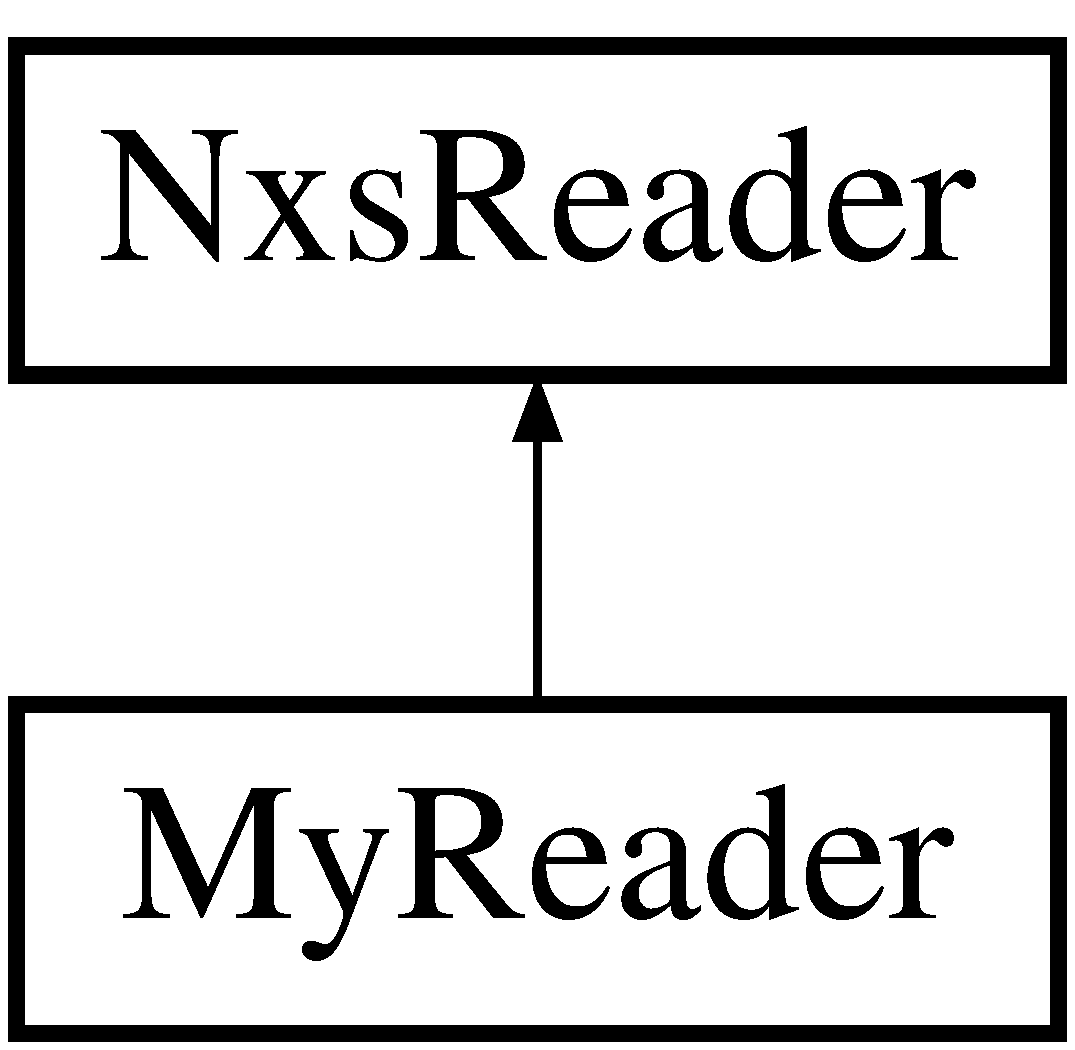
\includegraphics[height=2cm]{classMyReader}
\end{center}
\end{figure}
\subsection*{Public Member Functions}
\begin{DoxyCompactItemize}
\item 
\hyperlink{classMyReader_a739b792f1ac98c5a80720c13f34f2e31}{MyReader} (char $\ast$infname)
\item 
virtual \hyperlink{classMyReader_a16fff4945fbe5120e2ba761dbdf157dd}{$\sim$MyReader} ()
\item 
virtual void \hyperlink{classMyReader_a93ece63ab4306cf45f030b07395bc66e}{ExecuteStarting} ()
\item 
virtual void \hyperlink{classMyReader_aba1935daa8cec049934eb84822ddda4e}{ExecuteStopping} ()
\item 
virtual bool \hyperlink{classMyReader_a9ec496b979676b633003d5d3534c026c}{EnteringBlock} (\hyperlink{classNxsString}{NxsString} blockName)
\item 
virtual void \hyperlink{classMyReader_a81320d28a7b55fd8c56a949457640b99}{SkippingBlock} (\hyperlink{classNxsString}{NxsString} blockName)
\item 
virtual void \hyperlink{classMyReader_a0860a9670236993a197ace29278b0eea}{OutputComment} (const \hyperlink{classNxsString}{NxsString} \&comment)
\item 
virtual void \hyperlink{classMyReader_ad9cf686cdeb2e191cb5179094f723ef0}{NexusError} (\hyperlink{classNxsString}{NxsString} msg, file\_\-pos pos, long line, long col)
\end{DoxyCompactItemize}
\subsection*{Public Attributes}
\begin{DoxyCompactItemize}
\item 
ifstream \hyperlink{classMyReader_a324d60c6621c75e8ae83b4edab0344f8}{inf}
\end{DoxyCompactItemize}


\subsection{Detailed Description}
\hyperlink{classMyReader}{MyReader} class to make more informative message 

\subsection{Constructor \& Destructor Documentation}
\hypertarget{classMyReader_a739b792f1ac98c5a80720c13f34f2e31}{
\index{MyReader@{MyReader}!MyReader@{MyReader}}
\index{MyReader@{MyReader}!MyReader@{MyReader}}
\subsubsection[{MyReader}]{\setlength{\rightskip}{0pt plus 5cm}MyReader::MyReader (char $\ast$ {\em infname})\hspace{0.3cm}{\ttfamily  \mbox{[}inline\mbox{]}}}}
\label{classMyReader_a739b792f1ac98c5a80720c13f34f2e31}
constructor 
\begin{DoxyParams}{Parameters}
\item[{\em infname}]input file name \end{DoxyParams}
\hypertarget{classMyReader_a16fff4945fbe5120e2ba761dbdf157dd}{
\index{MyReader@{MyReader}!$\sim$MyReader@{$\sim$MyReader}}
\index{$\sim$MyReader@{$\sim$MyReader}!MyReader@{MyReader}}
\subsubsection[{$\sim$MyReader}]{\setlength{\rightskip}{0pt plus 5cm}virtual MyReader::$\sim$MyReader ()\hspace{0.3cm}{\ttfamily  \mbox{[}inline, virtual\mbox{]}}}}
\label{classMyReader_a16fff4945fbe5120e2ba761dbdf157dd}
destructor 

\subsection{Member Function Documentation}
\hypertarget{classMyReader_a9ec496b979676b633003d5d3534c026c}{
\index{MyReader@{MyReader}!EnteringBlock@{EnteringBlock}}
\index{EnteringBlock@{EnteringBlock}!MyReader@{MyReader}}
\subsubsection[{EnteringBlock}]{\setlength{\rightskip}{0pt plus 5cm}virtual bool MyReader::EnteringBlock ({\bf NxsString} {\em blockName})\hspace{0.3cm}{\ttfamily  \mbox{[}inline, virtual\mbox{]}}}}
\label{classMyReader_a9ec496b979676b633003d5d3534c026c}
enter a block 
\begin{DoxyParams}{Parameters}
\item[{\em blockName}]block name \end{DoxyParams}
\begin{DoxyReturn}{Returns}
true always 
\end{DoxyReturn}


Reimplemented from \hyperlink{classNxsReader}{NxsReader}.\hypertarget{classMyReader_a93ece63ab4306cf45f030b07395bc66e}{
\index{MyReader@{MyReader}!ExecuteStarting@{ExecuteStarting}}
\index{ExecuteStarting@{ExecuteStarting}!MyReader@{MyReader}}
\subsubsection[{ExecuteStarting}]{\setlength{\rightskip}{0pt plus 5cm}virtual void MyReader::ExecuteStarting ()\hspace{0.3cm}{\ttfamily  \mbox{[}inline, virtual\mbox{]}}}}
\label{classMyReader_a93ece63ab4306cf45f030b07395bc66e}
start 

Reimplemented from \hyperlink{classNxsReader}{NxsReader}.\hypertarget{classMyReader_aba1935daa8cec049934eb84822ddda4e}{
\index{MyReader@{MyReader}!ExecuteStopping@{ExecuteStopping}}
\index{ExecuteStopping@{ExecuteStopping}!MyReader@{MyReader}}
\subsubsection[{ExecuteStopping}]{\setlength{\rightskip}{0pt plus 5cm}virtual void MyReader::ExecuteStopping ()\hspace{0.3cm}{\ttfamily  \mbox{[}inline, virtual\mbox{]}}}}
\label{classMyReader_aba1935daa8cec049934eb84822ddda4e}
stop 

Reimplemented from \hyperlink{classNxsReader}{NxsReader}.\hypertarget{classMyReader_ad9cf686cdeb2e191cb5179094f723ef0}{
\index{MyReader@{MyReader}!NexusError@{NexusError}}
\index{NexusError@{NexusError}!MyReader@{MyReader}}
\subsubsection[{NexusError}]{\setlength{\rightskip}{0pt plus 5cm}virtual void MyReader::NexusError ({\bf NxsString} {\em msg}, \/  file\_\-pos {\em pos}, \/  long {\em line}, \/  long {\em col})\hspace{0.3cm}{\ttfamily  \mbox{[}inline, virtual\mbox{]}}}}
\label{classMyReader_ad9cf686cdeb2e191cb5179094f723ef0}
called when error occurs 
\begin{DoxyParams}{Parameters}
\item[{\em msg}]additional message \item[{\em pos}]file position \item[{\em line}]line number \item[{\em col}]column number \end{DoxyParams}


Reimplemented from \hyperlink{classNxsReader}{NxsReader}.\hypertarget{classMyReader_a0860a9670236993a197ace29278b0eea}{
\index{MyReader@{MyReader}!OutputComment@{OutputComment}}
\index{OutputComment@{OutputComment}!MyReader@{MyReader}}
\subsubsection[{OutputComment}]{\setlength{\rightskip}{0pt plus 5cm}virtual void MyReader::OutputComment (const {\bf NxsString} \& {\em comment})\hspace{0.3cm}{\ttfamily  \mbox{[}inline, virtual\mbox{]}}}}
\label{classMyReader_a0860a9670236993a197ace29278b0eea}
print comments 
\begin{DoxyParams}{Parameters}
\item[{\em comment}]comment string \end{DoxyParams}


Reimplemented from \hyperlink{classNxsReader}{NxsReader}.\hypertarget{classMyReader_a81320d28a7b55fd8c56a949457640b99}{
\index{MyReader@{MyReader}!SkippingBlock@{SkippingBlock}}
\index{SkippingBlock@{SkippingBlock}!MyReader@{MyReader}}
\subsubsection[{SkippingBlock}]{\setlength{\rightskip}{0pt plus 5cm}virtual void MyReader::SkippingBlock ({\bf NxsString} {\em blockName})\hspace{0.3cm}{\ttfamily  \mbox{[}inline, virtual\mbox{]}}}}
\label{classMyReader_a81320d28a7b55fd8c56a949457640b99}
skip a block 
\begin{DoxyParams}{Parameters}
\item[{\em blockName}]block name \end{DoxyParams}


Reimplemented from \hyperlink{classNxsReader}{NxsReader}.

\subsection{Member Data Documentation}
\hypertarget{classMyReader_a324d60c6621c75e8ae83b4edab0344f8}{
\index{MyReader@{MyReader}!inf@{inf}}
\index{inf@{inf}!MyReader@{MyReader}}
\subsubsection[{inf}]{\setlength{\rightskip}{0pt plus 5cm}ifstream {\bf MyReader::inf}}}
\label{classMyReader_a324d60c6621c75e8ae83b4edab0344f8}
input stream 

The documentation for this class was generated from the following file:\begin{DoxyCompactItemize}
\item 
src/myreader.h\end{DoxyCompactItemize}

\hypertarget{classMyToken}{
\section{MyToken Class Reference}
\label{classMyToken}\index{MyToken@{MyToken}}
}


{\ttfamily \#include $<$myreader.h$>$}Inheritance diagram for MyToken::\begin{figure}[H]
\begin{center}
\leavevmode
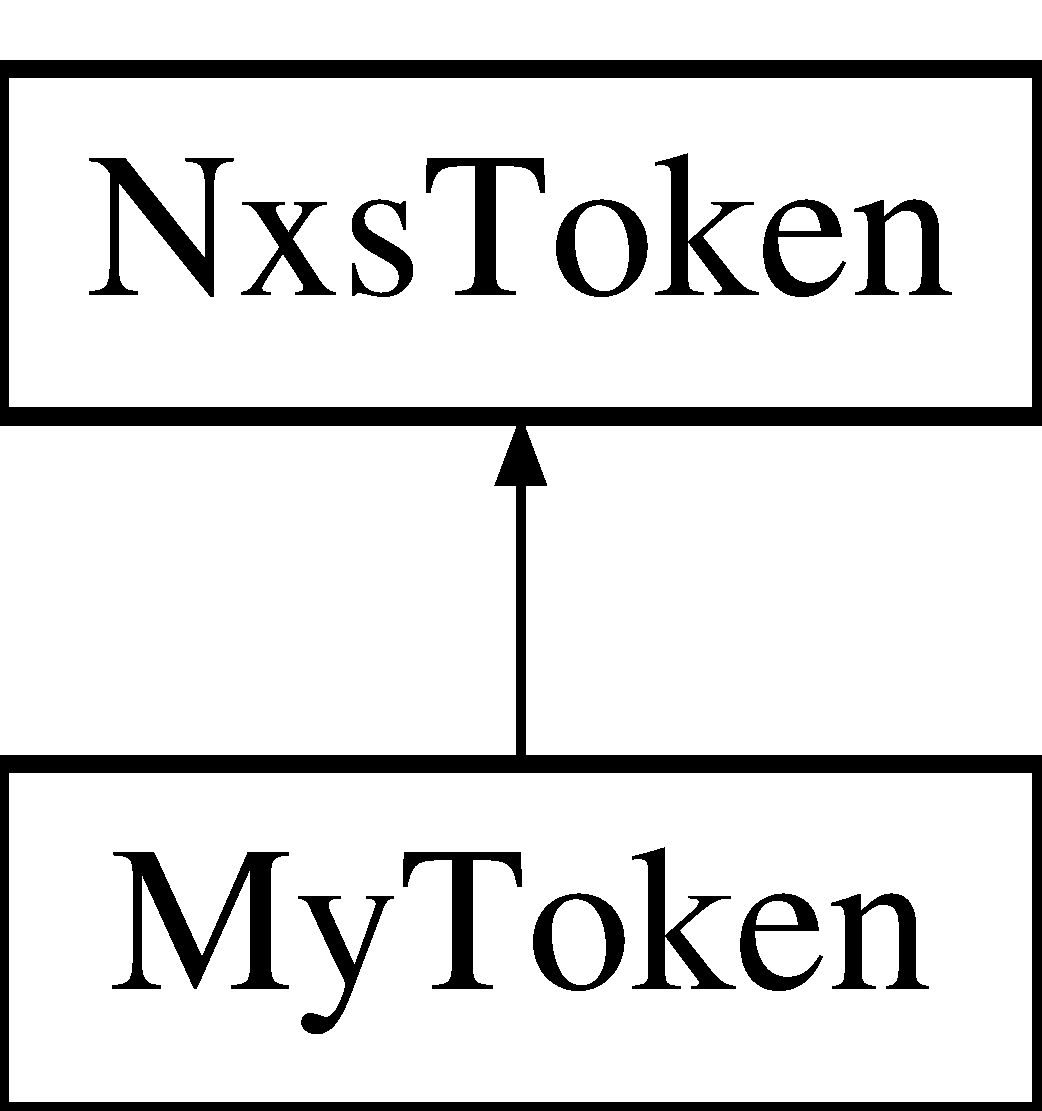
\includegraphics[height=2cm]{classMyToken}
\end{center}
\end{figure}
\subsection*{Public Member Functions}
\begin{DoxyCompactItemize}
\item 
\hyperlink{classMyToken_a617868499b04824c4ca84ba74cd7fc09}{MyToken} (istream \&is)
\item 
virtual void \hyperlink{classMyToken_a8b9a7b1c600e6d836c3f8e18a54cc71e}{OutputComment} (const \hyperlink{classNxsString}{NxsString} \&msg)
\end{DoxyCompactItemize}


\subsection{Detailed Description}
\hyperlink{classMyToken}{MyToken} class to make more informative message 

\subsection{Constructor \& Destructor Documentation}
\hypertarget{classMyToken_a617868499b04824c4ca84ba74cd7fc09}{
\index{MyToken@{MyToken}!MyToken@{MyToken}}
\index{MyToken@{MyToken}!MyToken@{MyToken}}
\subsubsection[{MyToken}]{\setlength{\rightskip}{0pt plus 5cm}MyToken::MyToken (istream \& {\em is})\hspace{0.3cm}{\ttfamily  \mbox{[}inline\mbox{]}}}}
\label{classMyToken_a617868499b04824c4ca84ba74cd7fc09}
constructor 
\begin{DoxyParams}{Parameters}
\item[{\em is}]input stream \end{DoxyParams}


\subsection{Member Function Documentation}
\hypertarget{classMyToken_a8b9a7b1c600e6d836c3f8e18a54cc71e}{
\index{MyToken@{MyToken}!OutputComment@{OutputComment}}
\index{OutputComment@{OutputComment}!MyToken@{MyToken}}
\subsubsection[{OutputComment}]{\setlength{\rightskip}{0pt plus 5cm}virtual void MyToken::OutputComment (const {\bf NxsString} \& {\em msg})\hspace{0.3cm}{\ttfamily  \mbox{[}inline, virtual\mbox{]}}}}
\label{classMyToken_a8b9a7b1c600e6d836c3f8e18a54cc71e}
print comments 
\begin{DoxyParams}{Parameters}
\item[{\em msg}]comment string \end{DoxyParams}


Reimplemented from \hyperlink{classNxsToken}{NxsToken}.

The documentation for this class was generated from the following file:\begin{DoxyCompactItemize}
\item 
src/myreader.h\end{DoxyCompactItemize}

\hypertarget{classNeighbor}{
\section{Neighbor Class Reference}
\label{classNeighbor}\index{Neighbor@{Neighbor}}
}


{\ttfamily \#include $<$node.h$>$}Inheritance diagram for Neighbor::\begin{figure}[H]
\begin{center}
\leavevmode
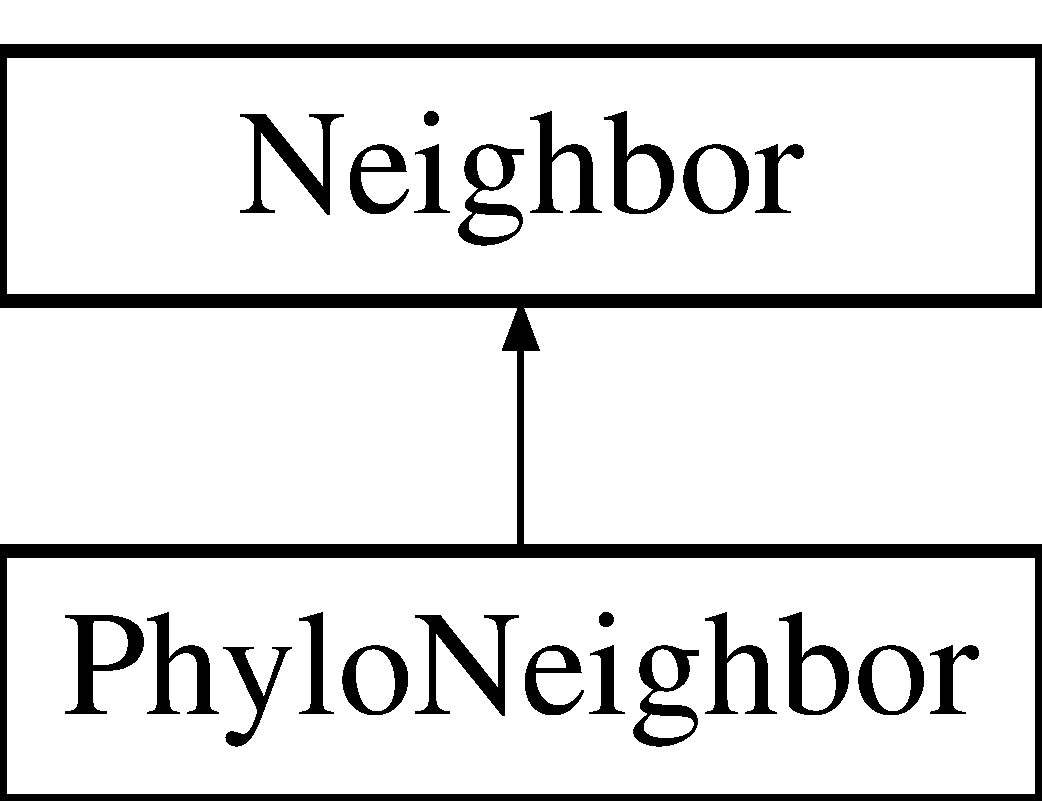
\includegraphics[height=2cm]{classNeighbor}
\end{center}
\end{figure}
\subsection*{Public Member Functions}
\begin{DoxyCompactItemize}
\item 
\hyperlink{classNeighbor_a5fce1b4b3ca5dc76bb7ba042b76786cb}{Neighbor} (\hyperlink{classNode}{Node} $\ast$anode, double alength)
\item 
\hyperlink{classNeighbor_aa93ef5611e62a5249e743465df3845ad}{Neighbor} (\hyperlink{classNeighbor}{Neighbor} $\ast$nei)
\item 
virtual \hyperlink{classNeighbor_a5dc94080d5904a504dfe3bcc7e9e14bb}{$\sim$Neighbor} ()
\end{DoxyCompactItemize}
\subsection*{Public Attributes}
\begin{DoxyCompactItemize}
\item 
\hyperlink{classNode}{Node} $\ast$ \hyperlink{classNeighbor_aa3e869eea994f6aa07708d3f326e01cb}{node}
\item 
double \hyperlink{classNeighbor_af6ad6ad901efea8b73bca889e2a0a501}{length}
\end{DoxyCompactItemize}


\subsection{Detailed Description}
\hyperlink{classNeighbor}{Neighbor} list of a node in the tree 

\subsection{Constructor \& Destructor Documentation}
\hypertarget{classNeighbor_a5fce1b4b3ca5dc76bb7ba042b76786cb}{
\index{Neighbor@{Neighbor}!Neighbor@{Neighbor}}
\index{Neighbor@{Neighbor}!Neighbor@{Neighbor}}
\subsubsection[{Neighbor}]{\setlength{\rightskip}{0pt plus 5cm}Neighbor::Neighbor ({\bf Node} $\ast$ {\em anode}, \/  double {\em alength})\hspace{0.3cm}{\ttfamily  \mbox{[}inline\mbox{]}}}}
\label{classNeighbor_a5fce1b4b3ca5dc76bb7ba042b76786cb}
construct class with a node and length 
\begin{DoxyParams}{Parameters}
\item[{\em anode}]the other end of the branch \item[{\em alength}]length of branch \end{DoxyParams}
\hypertarget{classNeighbor_aa93ef5611e62a5249e743465df3845ad}{
\index{Neighbor@{Neighbor}!Neighbor@{Neighbor}}
\index{Neighbor@{Neighbor}!Neighbor@{Neighbor}}
\subsubsection[{Neighbor}]{\setlength{\rightskip}{0pt plus 5cm}Neighbor::Neighbor ({\bf Neighbor} $\ast$ {\em nei})\hspace{0.3cm}{\ttfamily  \mbox{[}inline\mbox{]}}}}
\label{classNeighbor_aa93ef5611e62a5249e743465df3845ad}
construct class with another \hyperlink{classNeighbor}{Neighbor} 
\begin{DoxyParams}{Parameters}
\item[{\em nei}]another \hyperlink{classNeighbor}{Neighbor} \end{DoxyParams}
\hypertarget{classNeighbor_a5dc94080d5904a504dfe3bcc7e9e14bb}{
\index{Neighbor@{Neighbor}!$\sim$Neighbor@{$\sim$Neighbor}}
\index{$\sim$Neighbor@{$\sim$Neighbor}!Neighbor@{Neighbor}}
\subsubsection[{$\sim$Neighbor}]{\setlength{\rightskip}{0pt plus 5cm}virtual Neighbor::$\sim$Neighbor ()\hspace{0.3cm}{\ttfamily  \mbox{[}inline, virtual\mbox{]}}}}
\label{classNeighbor_a5dc94080d5904a504dfe3bcc7e9e14bb}
destructor 

\subsection{Member Data Documentation}
\hypertarget{classNeighbor_af6ad6ad901efea8b73bca889e2a0a501}{
\index{Neighbor@{Neighbor}!length@{length}}
\index{length@{length}!Neighbor@{Neighbor}}
\subsubsection[{length}]{\setlength{\rightskip}{0pt plus 5cm}double {\bf Neighbor::length}}}
\label{classNeighbor_af6ad6ad901efea8b73bca889e2a0a501}
branch length \hypertarget{classNeighbor_aa3e869eea994f6aa07708d3f326e01cb}{
\index{Neighbor@{Neighbor}!node@{node}}
\index{node@{node}!Neighbor@{Neighbor}}
\subsubsection[{node}]{\setlength{\rightskip}{0pt plus 5cm}{\bf Node}$\ast$ {\bf Neighbor::node}}}
\label{classNeighbor_aa3e869eea994f6aa07708d3f326e01cb}
the other end of the branch 

The documentation for this class was generated from the following file:\begin{DoxyCompactItemize}
\item 
src/node.h\end{DoxyCompactItemize}

\hypertarget{structneighborcmp}{
\section{neighborcmp Struct Reference}
\label{structneighborcmp}\index{neighborcmp@{neighborcmp}}
}


{\ttfamily \#include $<$node.h$>$}\subsection*{Public Member Functions}
\begin{DoxyCompactItemize}
\item 
bool \hyperlink{structneighborcmp_a9163b5610ba0f4e37061d88ecaeb2f6a}{operator()} (const \hyperlink{classNeighbor}{Neighbor} $\ast$s1, const \hyperlink{classNeighbor}{Neighbor} $\ast$s2) const 
\end{DoxyCompactItemize}


\subsection{Detailed Description}
\hyperlink{structneighborcmp}{neighborcmp}, for greedy algorithm 

\subsection{Member Function Documentation}
\hypertarget{structneighborcmp_a9163b5610ba0f4e37061d88ecaeb2f6a}{
\index{neighborcmp@{neighborcmp}!operator()@{operator()}}
\index{operator()@{operator()}!neighborcmp@{neighborcmp}}
\subsubsection[{operator()}]{\setlength{\rightskip}{0pt plus 5cm}bool neighborcmp::operator() (const {\bf Neighbor} $\ast$ {\em s1}, \/  const {\bf Neighbor} $\ast$ {\em s2}) const\hspace{0.3cm}{\ttfamily  \mbox{[}inline\mbox{]}}}}
\label{structneighborcmp_a9163b5610ba0f4e37061d88ecaeb2f6a}
\hyperlink{structneighborcmp}{neighborcmp}, for greedy algorithm 

The documentation for this struct was generated from the following file:\begin{DoxyCompactItemize}
\item 
src/node.h\end{DoxyCompactItemize}

\hypertarget{classNode}{
\section{Node Class Reference}
\label{classNode}\index{Node@{Node}}
}


{\ttfamily \#include $<$node.h$>$}Inheritance diagram for Node::\begin{figure}[H]
\begin{center}
\leavevmode
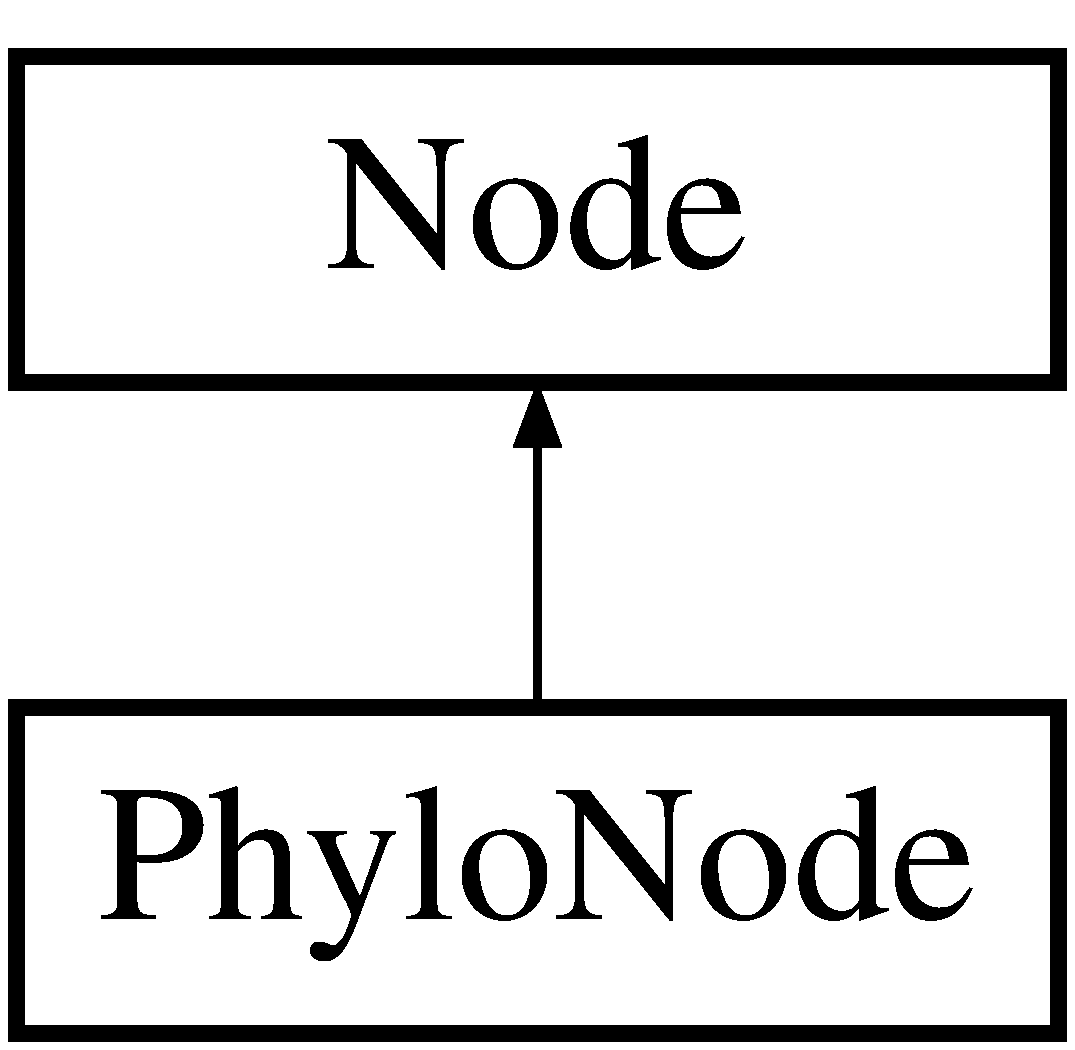
\includegraphics[height=2cm]{classNode}
\end{center}
\end{figure}
\subsection*{Public Member Functions}
\begin{DoxyCompactItemize}
\item 
\hyperlink{classNode_ad7a34779cad45d997bfd6d3d8043c75f}{Node} ()
\item 
\hyperlink{classNode_af6165e50e0ce42c0cfad89e62066be69}{Node} (int aid)
\item 
\hyperlink{classNode_a5161742d57505f425fb3f8b8ab0c883e}{Node} (int aid, int aname)
\item 
\hyperlink{classNode_aa8da7627c64a07c011e78cd71d9d5f8e}{Node} (int aid, const char $\ast$aname)
\item 
virtual \hyperlink{classNode_aa0840c3cb5c7159be6d992adecd2097c}{$\sim$Node} ()
\item 
virtual void \hyperlink{classNode_aaccc6f1874a0ddf07d281270d9f9c301}{deleteNode} ()
\item 
bool \hyperlink{classNode_a3a61dca67d5ad06cacb8c48eb6374973}{isLeaf} ()
\item 
int \hyperlink{classNode_a83a14e84b986038eb444e8945849d127}{degree} ()
\item 
\hyperlink{classNode}{Node} $\ast$ \hyperlink{classNode_a1340ab80fa547e2f09e766a4c327f387}{calcHeight} (\hyperlink{classNode}{Node} $\ast$dad=NULL)
\item 
double \hyperlink{classNode_a327b0ab1379f0dc6ad4062e3b253dd6f}{longestPath2} (\hyperlink{classNode}{Node} $\ast$\&node1, \hyperlink{classNode}{Node} $\ast$\&node2)
\item 
\hyperlink{classNeighbor}{Neighbor} $\ast$ \hyperlink{classNode_a522b44457c22e6c97e7becfec43cbdba}{findNeighbor} (\hyperlink{classNode}{Node} $\ast$node)
\item 
NeighborVec::iterator \hyperlink{classNode_acb2b4563be11a48ec1503bb22a56893a}{findNeighborIt} (\hyperlink{classNode}{Node} $\ast$node)
\item 
void \hyperlink{classNode_a991931db235cedbcdae20bcb77a57671}{updateNeighbor} (\hyperlink{classNode}{Node} $\ast$node, \hyperlink{classNode}{Node} $\ast$newnode, double newlen)
\item 
double \hyperlink{classNode_ac0dce50c1942b6c015fb8a10695dcc5a}{updateNeighbor} (\hyperlink{classNode}{Node} $\ast$node, \hyperlink{classNode}{Node} $\ast$newnode)
\item 
void \hyperlink{classNode_ab45fa6addf881a2c6c090bbd9686710f}{updateNeighbor} (NeighborVec::iterator nei\_\-it, \hyperlink{classNeighbor}{Neighbor} $\ast$newnei)
\item 
void \hyperlink{classNode_a60ae4ce857e2ed5c3115060eeeec405b}{updateNeighbor} (NeighborVec::iterator nei\_\-it, \hyperlink{classNeighbor}{Neighbor} $\ast$newnei, double newlen)
\item 
void \hyperlink{classNode_a7939f3acf93cb262bfea402e7c81bc87}{updateNeighbor} (\hyperlink{classNode}{Node} $\ast$node, \hyperlink{classNeighbor}{Neighbor} $\ast$newnei)
\item 
void \hyperlink{classNode_a0994f789ab4030889f70e5b69bcc57b3}{updateNeighbor} (\hyperlink{classNode}{Node} $\ast$node, \hyperlink{classNeighbor}{Neighbor} $\ast$newnei, double newlen)
\item 
virtual void \hyperlink{classNode_abd8e9dbecc4ad76fdebefbb1b578b6f0}{addNeighbor} (\hyperlink{classNode}{Node} $\ast$node, double length)
\end{DoxyCompactItemize}
\subsection*{Public Attributes}
\begin{DoxyCompactItemize}
\item 
int \hyperlink{classNode_a59a543130a10c95f1e8642cf8c5645e8}{id}
\item 
\hyperlink{classNxsString}{NxsString} \hyperlink{classNode_a57c014f7366ed417746d92336d869510}{name}
\item 
NeighborVec \hyperlink{classNode_a35de03872f10f71851fe4c115a981d93}{neighbors}
\item 
double \hyperlink{classNode_aa0f22093957939b69e2872893ac6bccd}{height}
\item 
\hyperlink{classNeighbor}{Neighbor} $\ast$ \hyperlink{classNode_a2683e662b7577fbd5a5b78a9d2976a17}{highestNei}
\end{DoxyCompactItemize}


\subsection{Detailed Description}
A \hyperlink{classNode}{Node} in the tree \begin{DoxyAuthor}{Author}
BUI Quang Minh, Steffen Klaere, Arndt von Haeseler 
\end{DoxyAuthor}


\subsection{Constructor \& Destructor Documentation}
\hypertarget{classNode_ad7a34779cad45d997bfd6d3d8043c75f}{
\index{Node@{Node}!Node@{Node}}
\index{Node@{Node}!Node@{Node}}
\subsubsection[{Node}]{\setlength{\rightskip}{0pt plus 5cm}Node::Node ()\hspace{0.3cm}{\ttfamily  \mbox{[}inline\mbox{]}}}}
\label{classNode_ad7a34779cad45d997bfd6d3d8043c75f}
constructor \hypertarget{classNode_af6165e50e0ce42c0cfad89e62066be69}{
\index{Node@{Node}!Node@{Node}}
\index{Node@{Node}!Node@{Node}}
\subsubsection[{Node}]{\setlength{\rightskip}{0pt plus 5cm}Node::Node (int {\em aid})}}
\label{classNode_af6165e50e0ce42c0cfad89e62066be69}
constructor 
\begin{DoxyParams}{Parameters}
\item[{\em aid}]id of this node \end{DoxyParams}
\hypertarget{classNode_a5161742d57505f425fb3f8b8ab0c883e}{
\index{Node@{Node}!Node@{Node}}
\index{Node@{Node}!Node@{Node}}
\subsubsection[{Node}]{\setlength{\rightskip}{0pt plus 5cm}Node::Node (int {\em aid}, \/  int {\em aname})}}
\label{classNode_a5161742d57505f425fb3f8b8ab0c883e}
constructor 
\begin{DoxyParams}{Parameters}
\item[{\em aid}]id of this node \item[{\em aname}]name of this node \end{DoxyParams}
\hypertarget{classNode_aa8da7627c64a07c011e78cd71d9d5f8e}{
\index{Node@{Node}!Node@{Node}}
\index{Node@{Node}!Node@{Node}}
\subsubsection[{Node}]{\setlength{\rightskip}{0pt plus 5cm}Node::Node (int {\em aid}, \/  const char $\ast$ {\em aname})}}
\label{classNode_aa8da7627c64a07c011e78cd71d9d5f8e}
constructor 
\begin{DoxyParams}{Parameters}
\item[{\em aid}]id of this node \item[{\em aname}]name of this node \end{DoxyParams}
\hypertarget{classNode_aa0840c3cb5c7159be6d992adecd2097c}{
\index{Node@{Node}!$\sim$Node@{$\sim$Node}}
\index{$\sim$Node@{$\sim$Node}!Node@{Node}}
\subsubsection[{$\sim$Node}]{\setlength{\rightskip}{0pt plus 5cm}Node::$\sim$Node ()\hspace{0.3cm}{\ttfamily  \mbox{[}virtual\mbox{]}}}}
\label{classNode_aa0840c3cb5c7159be6d992adecd2097c}
destructor 

\subsection{Member Function Documentation}
\hypertarget{classNode_abd8e9dbecc4ad76fdebefbb1b578b6f0}{
\index{Node@{Node}!addNeighbor@{addNeighbor}}
\index{addNeighbor@{addNeighbor}!Node@{Node}}
\subsubsection[{addNeighbor}]{\setlength{\rightskip}{0pt plus 5cm}void Node::addNeighbor ({\bf Node} $\ast$ {\em node}, \/  double {\em length})\hspace{0.3cm}{\ttfamily  \mbox{[}virtual\mbox{]}}}}
\label{classNode_abd8e9dbecc4ad76fdebefbb1b578b6f0}
add a neighbor 
\begin{DoxyParams}{Parameters}
\item[{\em node}]the neighbor node \item[{\em length}]branch length \end{DoxyParams}
\hypertarget{classNode_a1340ab80fa547e2f09e766a4c327f387}{
\index{Node@{Node}!calcHeight@{calcHeight}}
\index{calcHeight@{calcHeight}!Node@{Node}}
\subsubsection[{calcHeight}]{\setlength{\rightskip}{0pt plus 5cm}{\bf Node} $\ast$ Node::calcHeight ({\bf Node} $\ast$ {\em dad} = {\ttfamily NULL})}}
\label{classNode_a1340ab80fa547e2f09e766a4c327f387}
calculate the height of the subtree rooted at this node, given the dad. Also return the lowestLeaf. 
\begin{DoxyParams}{Parameters}
\item[{\em dad}]the dad of this node \end{DoxyParams}
\begin{DoxyReturn}{Returns}
the leaf at the lowest level. Also modify the height, highestNei of this class. 
\end{DoxyReturn}
\hypertarget{classNode_a83a14e84b986038eb444e8945849d127}{
\index{Node@{Node}!degree@{degree}}
\index{degree@{degree}!Node@{Node}}
\subsubsection[{degree}]{\setlength{\rightskip}{0pt plus 5cm}int Node::degree ()}}
\label{classNode_a83a14e84b986038eb444e8945849d127}
\begin{DoxyReturn}{Returns}
the number of adjacent nodes 
\end{DoxyReturn}
\hypertarget{classNode_aaccc6f1874a0ddf07d281270d9f9c301}{
\index{Node@{Node}!deleteNode@{deleteNode}}
\index{deleteNode@{deleteNode}!Node@{Node}}
\subsubsection[{deleteNode}]{\setlength{\rightskip}{0pt plus 5cm}void Node::deleteNode ()\hspace{0.3cm}{\ttfamily  \mbox{[}virtual\mbox{]}}}}
\label{classNode_aaccc6f1874a0ddf07d281270d9f9c301}
used for the destructor \hypertarget{classNode_a522b44457c22e6c97e7becfec43cbdba}{
\index{Node@{Node}!findNeighbor@{findNeighbor}}
\index{findNeighbor@{findNeighbor}!Node@{Node}}
\subsubsection[{findNeighbor}]{\setlength{\rightskip}{0pt plus 5cm}{\bf Neighbor} $\ast$ Node::findNeighbor ({\bf Node} $\ast$ {\em node})}}
\label{classNode_a522b44457c22e6c97e7becfec43cbdba}

\begin{DoxyParams}{Parameters}
\item[{\em node}]the target node \end{DoxyParams}
\begin{DoxyReturn}{Returns}
the iterator to the neighbor that has the node. If not found, return NULL 
\end{DoxyReturn}
\hypertarget{classNode_acb2b4563be11a48ec1503bb22a56893a}{
\index{Node@{Node}!findNeighborIt@{findNeighborIt}}
\index{findNeighborIt@{findNeighborIt}!Node@{Node}}
\subsubsection[{findNeighborIt}]{\setlength{\rightskip}{0pt plus 5cm}NeighborVec::iterator Node::findNeighborIt ({\bf Node} $\ast$ {\em node})}}
\label{classNode_acb2b4563be11a48ec1503bb22a56893a}

\begin{DoxyParams}{Parameters}
\item[{\em node}]the target node \end{DoxyParams}
\begin{DoxyReturn}{Returns}
the iterator to the neighbor that has the node. If not found, return neighbors.end() 
\end{DoxyReturn}
\hypertarget{classNode_a3a61dca67d5ad06cacb8c48eb6374973}{
\index{Node@{Node}!isLeaf@{isLeaf}}
\index{isLeaf@{isLeaf}!Node@{Node}}
\subsubsection[{isLeaf}]{\setlength{\rightskip}{0pt plus 5cm}bool Node::isLeaf ()}}
\label{classNode_a3a61dca67d5ad06cacb8c48eb6374973}
\begin{DoxyReturn}{Returns}
true of this is a leaf 
\end{DoxyReturn}
\hypertarget{classNode_a327b0ab1379f0dc6ad4062e3b253dd6f}{
\index{Node@{Node}!longestPath2@{longestPath2}}
\index{longestPath2@{longestPath2}!Node@{Node}}
\subsubsection[{longestPath2}]{\setlength{\rightskip}{0pt plus 5cm}double Node::longestPath2 ({\bf Node} $\ast$\& {\em node1}, \/  {\bf Node} $\ast$\& {\em node2})}}
\label{classNode_a327b0ab1379f0dc6ad4062e3b253dd6f}
calculate the longest path in the subtree (version 2: more efficient) 
\begin{DoxyParams}{Parameters}
\item[{\em node1}]the returned node1 of the one end of the path \item[{\em node2}]the returned node2 of the one end of the path \end{DoxyParams}
\begin{DoxyReturn}{Returns}
the length of the longest path
\end{DoxyReturn}
efficient longest path algorithm \hypertarget{classNode_a0994f789ab4030889f70e5b69bcc57b3}{
\index{Node@{Node}!updateNeighbor@{updateNeighbor}}
\index{updateNeighbor@{updateNeighbor}!Node@{Node}}
\subsubsection[{updateNeighbor}]{\setlength{\rightskip}{0pt plus 5cm}void Node::updateNeighbor ({\bf Node} $\ast$ {\em node}, \/  {\bf Neighbor} $\ast$ {\em newnei}, \/  double {\em newlen})}}
\label{classNode_a0994f789ab4030889f70e5b69bcc57b3}
update the neighbor node with the newnode 
\begin{DoxyParams}{Parameters}
\item[{\em node}]old neighbor node \item[{\em newnei}]new neighbor \item[{\em newlen}]new branch length \end{DoxyParams}
\hypertarget{classNode_a7939f3acf93cb262bfea402e7c81bc87}{
\index{Node@{Node}!updateNeighbor@{updateNeighbor}}
\index{updateNeighbor@{updateNeighbor}!Node@{Node}}
\subsubsection[{updateNeighbor}]{\setlength{\rightskip}{0pt plus 5cm}void Node::updateNeighbor ({\bf Node} $\ast$ {\em node}, \/  {\bf Neighbor} $\ast$ {\em newnei})}}
\label{classNode_a7939f3acf93cb262bfea402e7c81bc87}
update the neighbor node with the newnode 
\begin{DoxyParams}{Parameters}
\item[{\em node}]old neighbor node \item[{\em newnei}]new neighbor \end{DoxyParams}
\hypertarget{classNode_a60ae4ce857e2ed5c3115060eeeec405b}{
\index{Node@{Node}!updateNeighbor@{updateNeighbor}}
\index{updateNeighbor@{updateNeighbor}!Node@{Node}}
\subsubsection[{updateNeighbor}]{\setlength{\rightskip}{0pt plus 5cm}void Node::updateNeighbor (NeighborVec::iterator {\em nei\_\-it}, \/  {\bf Neighbor} $\ast$ {\em newnei}, \/  double {\em newlen})}}
\label{classNode_a60ae4ce857e2ed5c3115060eeeec405b}
update the neighbor node with the newnode 
\begin{DoxyParams}{Parameters}
\item[{\em nei\_\-it}]iterator to the neighbor \item[{\em newnei}]new neighbor \item[{\em newlen}]new branch length \end{DoxyParams}
\hypertarget{classNode_ab45fa6addf881a2c6c090bbd9686710f}{
\index{Node@{Node}!updateNeighbor@{updateNeighbor}}
\index{updateNeighbor@{updateNeighbor}!Node@{Node}}
\subsubsection[{updateNeighbor}]{\setlength{\rightskip}{0pt plus 5cm}void Node::updateNeighbor (NeighborVec::iterator {\em nei\_\-it}, \/  {\bf Neighbor} $\ast$ {\em newnei})}}
\label{classNode_ab45fa6addf881a2c6c090bbd9686710f}
update the neighbor node with the newnode 
\begin{DoxyParams}{Parameters}
\item[{\em nei\_\-it}]iterator to the neighbor \item[{\em newnei}]new neighbor \end{DoxyParams}
\hypertarget{classNode_ac0dce50c1942b6c015fb8a10695dcc5a}{
\index{Node@{Node}!updateNeighbor@{updateNeighbor}}
\index{updateNeighbor@{updateNeighbor}!Node@{Node}}
\subsubsection[{updateNeighbor}]{\setlength{\rightskip}{0pt plus 5cm}double Node::updateNeighbor ({\bf Node} $\ast$ {\em node}, \/  {\bf Node} $\ast$ {\em newnode})}}
\label{classNode_ac0dce50c1942b6c015fb8a10695dcc5a}
update the neighbor node with the newnode 
\begin{DoxyParams}{Parameters}
\item[{\em node}]old neighbor node \item[{\em newnode}]new neighbor node \end{DoxyParams}
\begin{DoxyReturn}{Returns}
length applied for the corresponding branch 
\end{DoxyReturn}
\hypertarget{classNode_a991931db235cedbcdae20bcb77a57671}{
\index{Node@{Node}!updateNeighbor@{updateNeighbor}}
\index{updateNeighbor@{updateNeighbor}!Node@{Node}}
\subsubsection[{updateNeighbor}]{\setlength{\rightskip}{0pt plus 5cm}void Node::updateNeighbor ({\bf Node} $\ast$ {\em node}, \/  {\bf Node} $\ast$ {\em newnode}, \/  double {\em newlen})}}
\label{classNode_a991931db235cedbcdae20bcb77a57671}
update the neighbor node with the newnode 
\begin{DoxyParams}{Parameters}
\item[{\em node}]old neighbor node \item[{\em newnode}]new neighbor node \item[{\em newlen}]new length applied for the corresponding branch \end{DoxyParams}


\subsection{Member Data Documentation}
\hypertarget{classNode_aa0f22093957939b69e2872893ac6bccd}{
\index{Node@{Node}!height@{height}}
\index{height@{height}!Node@{Node}}
\subsubsection[{height}]{\setlength{\rightskip}{0pt plus 5cm}double {\bf Node::height}}}
\label{classNode_aa0f22093957939b69e2872893ac6bccd}
the height of subtree rooted at this node, used for greedy algorithm \hypertarget{classNode_a2683e662b7577fbd5a5b78a9d2976a17}{
\index{Node@{Node}!highestNei@{highestNei}}
\index{highestNei@{highestNei}!Node@{Node}}
\subsubsection[{highestNei}]{\setlength{\rightskip}{0pt plus 5cm}{\bf Neighbor}$\ast$ {\bf Node::highestNei}}}
\label{classNode_a2683e662b7577fbd5a5b78a9d2976a17}
child of maximal height of subtree rooted at this node, used for greedy algorithm \hypertarget{classNode_a59a543130a10c95f1e8642cf8c5645e8}{
\index{Node@{Node}!id@{id}}
\index{id@{id}!Node@{Node}}
\subsubsection[{id}]{\setlength{\rightskip}{0pt plus 5cm}int {\bf Node::id}}}
\label{classNode_a59a543130a10c95f1e8642cf8c5645e8}
node id. \hypertarget{classNode_a57c014f7366ed417746d92336d869510}{
\index{Node@{Node}!name@{name}}
\index{name@{name}!Node@{Node}}
\subsubsection[{name}]{\setlength{\rightskip}{0pt plus 5cm}{\bf NxsString} {\bf Node::name}}}
\label{classNode_a57c014f7366ed417746d92336d869510}
node name \hypertarget{classNode_a35de03872f10f71851fe4c115a981d93}{
\index{Node@{Node}!neighbors@{neighbors}}
\index{neighbors@{neighbors}!Node@{Node}}
\subsubsection[{neighbors}]{\setlength{\rightskip}{0pt plus 5cm}NeighborVec {\bf Node::neighbors}}}
\label{classNode_a35de03872f10f71851fe4c115a981d93}
list of neighbors 

The documentation for this class was generated from the following files:\begin{DoxyCompactItemize}
\item 
src/node.h\item 
src/node.cpp\end{DoxyCompactItemize}

\hypertarget{structnodecmp}{
\section{nodecmp Struct Reference}
\label{structnodecmp}\index{nodecmp@{nodecmp}}
}


{\ttfamily \#include $<$node.h$>$}\subsection*{Public Member Functions}
\begin{DoxyCompactItemize}
\item 
bool \hyperlink{structnodecmp_a1125c1d530d06317a559aade3744bc78}{operator()} (const \hyperlink{classNode}{Node} $\ast$s1, const \hyperlink{classNode}{Node} $\ast$s2) const 
\end{DoxyCompactItemize}


\subsection{Detailed Description}
\hyperlink{structnodecmp}{nodecmp}, for pruning algorithm 

\subsection{Member Function Documentation}
\hypertarget{structnodecmp_a1125c1d530d06317a559aade3744bc78}{
\index{nodecmp@{nodecmp}!operator()@{operator()}}
\index{operator()@{operator()}!nodecmp@{nodecmp}}
\subsubsection[{operator()}]{\setlength{\rightskip}{0pt plus 5cm}bool nodecmp::operator() (const {\bf Node} $\ast$ {\em s1}, \/  const {\bf Node} $\ast$ {\em s2}) const\hspace{0.3cm}{\ttfamily  \mbox{[}inline\mbox{]}}}}
\label{structnodecmp_a1125c1d530d06317a559aade3744bc78}
\hyperlink{structnodecmp}{nodecmp}, for pruning algorithm 

The documentation for this struct was generated from the following file:\begin{DoxyCompactItemize}
\item 
src/node.h\end{DoxyCompactItemize}

\hypertarget{structnodeheightcmp}{
\section{nodeheightcmp Struct Reference}
\label{structnodeheightcmp}\index{nodeheightcmp@{nodeheightcmp}}
}


{\ttfamily \#include $<$iqptree.h$>$}\subsection*{Public Member Functions}
\begin{DoxyCompactItemize}
\item 
bool \hyperlink{structnodeheightcmp_ae30bce4c8c8585e4250e18cdaf51d740}{operator()} (const \hyperlink{classNode}{Node} $\ast$s1, const \hyperlink{classNode}{Node} $\ast$s2) const 
\end{DoxyCompactItemize}


\subsection{Detailed Description}
\hyperlink{structnodeheightcmp}{nodeheightcmp}, for building k-\/representative leaf set 

\subsection{Member Function Documentation}
\hypertarget{structnodeheightcmp_ae30bce4c8c8585e4250e18cdaf51d740}{
\index{nodeheightcmp@{nodeheightcmp}!operator()@{operator()}}
\index{operator()@{operator()}!nodeheightcmp@{nodeheightcmp}}
\subsubsection[{operator()}]{\setlength{\rightskip}{0pt plus 5cm}bool nodeheightcmp::operator() (const {\bf Node} $\ast$ {\em s1}, \/  const {\bf Node} $\ast$ {\em s2}) const\hspace{0.3cm}{\ttfamily  \mbox{[}inline\mbox{]}}}}
\label{structnodeheightcmp_ae30bce4c8c8585e4250e18cdaf51d740}
\hyperlink{structnodeheightcmp}{nodeheightcmp}, for building k-\/representative leaf set 

The documentation for this struct was generated from the following file:\begin{DoxyCompactItemize}
\item 
src/iqptree.h\end{DoxyCompactItemize}

\hypertarget{classNStrCaseInsensitiveEquals}{
\section{NStrCaseInsensitiveEquals Class Reference}
\label{classNStrCaseInsensitiveEquals}\index{NStrCaseInsensitiveEquals@{NStrCaseInsensitiveEquals}}
}
\subsection*{Public Member Functions}
\begin{DoxyCompactItemize}
\item 
\hypertarget{classNStrCaseInsensitiveEquals_a07277f6ad9a09a10fa51894fe99909d3}{
{\bfseries NStrCaseInsensitiveEquals} (const \hyperlink{classNxsString}{NxsString} \&s)}
\label{classNStrCaseInsensitiveEquals_a07277f6ad9a09a10fa51894fe99909d3}

\item 
\hypertarget{classNStrCaseInsensitiveEquals_ab0538585efbf2bf3195b47a7a014a49c}{
bool {\bfseries operator()} (const \hyperlink{classNxsString}{NxsString} \&s)}
\label{classNStrCaseInsensitiveEquals_ab0538585efbf2bf3195b47a7a014a49c}

\end{DoxyCompactItemize}
\subsection*{Protected Attributes}
\begin{DoxyCompactItemize}
\item 
\hypertarget{classNStrCaseInsensitiveEquals_ad9362da48b09a005c82612ee3d8b6840}{
\hyperlink{classNxsString}{NxsString} {\bfseries compStr}}
\label{classNStrCaseInsensitiveEquals_ad9362da48b09a005c82612ee3d8b6840}

\end{DoxyCompactItemize}


The documentation for this class was generated from the following file:\begin{DoxyCompactItemize}
\item 
src/ncl/nxsstring.h\end{DoxyCompactItemize}

\hypertarget{classNStrCaseSensitiveEquals}{
\section{NStrCaseSensitiveEquals Class Reference}
\label{classNStrCaseSensitiveEquals}\index{NStrCaseSensitiveEquals@{NStrCaseSensitiveEquals}}
}
\subsection*{Public Member Functions}
\begin{DoxyCompactItemize}
\item 
\hypertarget{classNStrCaseSensitiveEquals_ad58017adf2d891883fb6276f4abc7314}{
{\bfseries NStrCaseSensitiveEquals} (const \hyperlink{classNxsString}{NxsString} \&s)}
\label{classNStrCaseSensitiveEquals_ad58017adf2d891883fb6276f4abc7314}

\item 
\hypertarget{classNStrCaseSensitiveEquals_a0917aae2b04a80ab0a6e5f780d4b3d79}{
bool {\bfseries operator()} (const \hyperlink{classNxsString}{NxsString} \&s) const }
\label{classNStrCaseSensitiveEquals_a0917aae2b04a80ab0a6e5f780d4b3d79}

\end{DoxyCompactItemize}
\subsection*{Protected Attributes}
\begin{DoxyCompactItemize}
\item 
\hypertarget{classNStrCaseSensitiveEquals_a3a3722574f9268f9c3009a53adb7123f}{
\hyperlink{classNxsString}{NxsString} {\bfseries compStr}}
\label{classNStrCaseSensitiveEquals_a3a3722574f9268f9c3009a53adb7123f}

\end{DoxyCompactItemize}


The documentation for this class was generated from the following file:\begin{DoxyCompactItemize}
\item 
src/ncl/nxsstring.h\end{DoxyCompactItemize}

\hypertarget{classNxsAssumptionsBlock}{
\section{NxsAssumptionsBlock Class Reference}
\label{classNxsAssumptionsBlock}\index{NxsAssumptionsBlock@{NxsAssumptionsBlock}}
}
Inheritance diagram for NxsAssumptionsBlock::\begin{figure}[H]
\begin{center}
\leavevmode
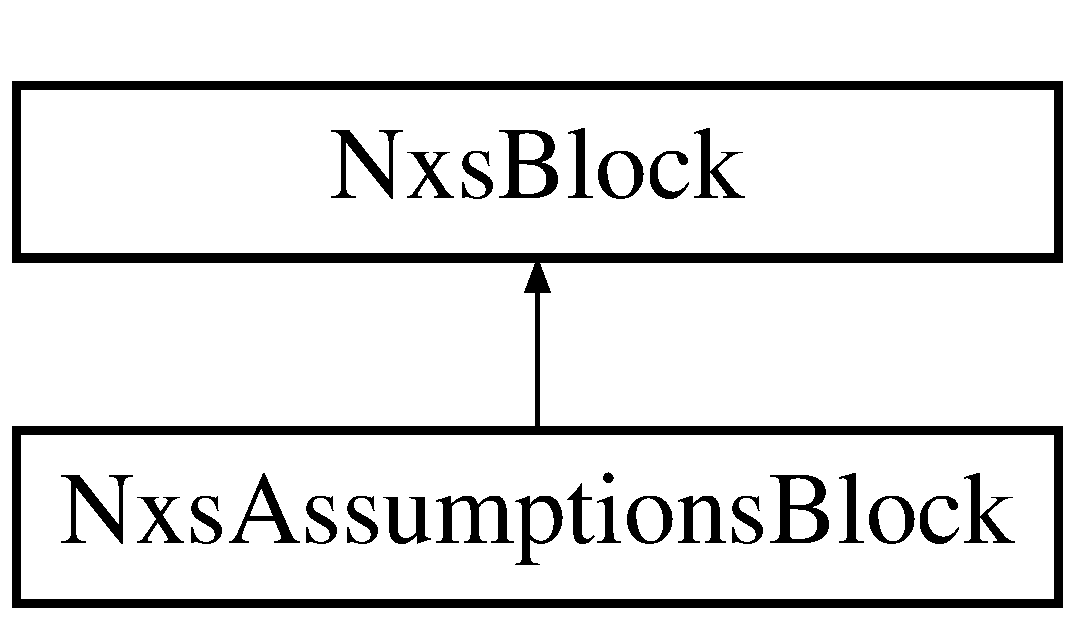
\includegraphics[height=2cm]{classNxsAssumptionsBlock}
\end{center}
\end{figure}
\subsection*{Public Member Functions}
\begin{DoxyCompactItemize}
\item 
\hypertarget{classNxsAssumptionsBlock_a1c91eb5774685b8876250056f08bf3a2}{
{\bfseries NxsAssumptionsBlock} (\hyperlink{classNxsTaxaBlock}{NxsTaxaBlock} $\ast$t)}
\label{classNxsAssumptionsBlock_a1c91eb5774685b8876250056f08bf3a2}

\item 
\hypertarget{classNxsAssumptionsBlock_a18237c0576ffeee41fca0deabc73a743}{
void {\bfseries ReplaceTaxaBlockPtr} (\hyperlink{classNxsTaxaBlock}{NxsTaxaBlock} $\ast$tb)}
\label{classNxsAssumptionsBlock_a18237c0576ffeee41fca0deabc73a743}

\item 
\hypertarget{classNxsAssumptionsBlock_a7eb13fdafe622c0a114bc9f4d9426ea3}{
void {\bfseries SetCallback} (\hyperlink{classNxsCharactersBlock}{NxsCharactersBlock} $\ast$p)}
\label{classNxsAssumptionsBlock_a7eb13fdafe622c0a114bc9f4d9426ea3}

\item 
\hypertarget{classNxsAssumptionsBlock_a65424f0588dc3d77834f6b3f1bc61867}{
int {\bfseries GetNumCharSets} ()}
\label{classNxsAssumptionsBlock_a65424f0588dc3d77834f6b3f1bc61867}

\item 
\hypertarget{classNxsAssumptionsBlock_a4dc4bd89b848a1ffc86b054cc7d6601c}{
void {\bfseries GetCharSetNames} (NxsStringVector \&names)}
\label{classNxsAssumptionsBlock_a4dc4bd89b848a1ffc86b054cc7d6601c}

\item 
\hypertarget{classNxsAssumptionsBlock_abefd0efc65f9cddf675166060df1ccce}{
NxsUnsignedSet \& {\bfseries GetCharSet} (\hyperlink{classNxsString}{NxsString} nm)}
\label{classNxsAssumptionsBlock_abefd0efc65f9cddf675166060df1ccce}

\item 
\hypertarget{classNxsAssumptionsBlock_a7336b168163deaf0fd20cb918498785c}{
\hyperlink{classNxsString}{NxsString} {\bfseries GetDefCharSetName} ()}
\label{classNxsAssumptionsBlock_a7336b168163deaf0fd20cb918498785c}

\item 
\hypertarget{classNxsAssumptionsBlock_aead6a4a2ddb3894003d32af95a45465b}{
int {\bfseries GetNumTaxSets} ()}
\label{classNxsAssumptionsBlock_aead6a4a2ddb3894003d32af95a45465b}

\item 
\hypertarget{classNxsAssumptionsBlock_a26f2fa28d0797b832dfaebe29e5a5e2e}{
void {\bfseries GetTaxSetNames} (NxsStringVector \&names)}
\label{classNxsAssumptionsBlock_a26f2fa28d0797b832dfaebe29e5a5e2e}

\item 
\hypertarget{classNxsAssumptionsBlock_a77edaa6ed625e35f6cab8c8f2ff85f08}{
NxsUnsignedSet \& {\bfseries GetTaxSet} (\hyperlink{classNxsString}{NxsString} nm)}
\label{classNxsAssumptionsBlock_a77edaa6ed625e35f6cab8c8f2ff85f08}

\item 
\hypertarget{classNxsAssumptionsBlock_a6a5f666ad93a34e92731810ab566b1d7}{
\hyperlink{classNxsString}{NxsString} {\bfseries GetDefTaxSetName} ()}
\label{classNxsAssumptionsBlock_a6a5f666ad93a34e92731810ab566b1d7}

\item 
\hypertarget{classNxsAssumptionsBlock_ab0cb9b501b0e4698df204c243352caeb}{
int {\bfseries GetNumExSets} ()}
\label{classNxsAssumptionsBlock_ab0cb9b501b0e4698df204c243352caeb}

\item 
\hypertarget{classNxsAssumptionsBlock_a858efae26b2eff355b5240405493f057}{
void {\bfseries GetExSetNames} (NxsStringVector \&names)}
\label{classNxsAssumptionsBlock_a858efae26b2eff355b5240405493f057}

\item 
\hypertarget{classNxsAssumptionsBlock_ab3e975170b5b3f292cb4d9de01297f43}{
NxsUnsignedSet \& {\bfseries GetExSet} (\hyperlink{classNxsString}{NxsString} nm)}
\label{classNxsAssumptionsBlock_ab3e975170b5b3f292cb4d9de01297f43}

\item 
\hypertarget{classNxsAssumptionsBlock_a008b67365008523a422529f45d1d070e}{
\hyperlink{classNxsString}{NxsString} {\bfseries GetDefExSetName} ()}
\label{classNxsAssumptionsBlock_a008b67365008523a422529f45d1d070e}

\item 
\hypertarget{classNxsAssumptionsBlock_a9d4a7bf784a6a97d1df06a88c0082459}{
void {\bfseries ApplyExSet} (\hyperlink{classNxsString}{NxsString} nm)}
\label{classNxsAssumptionsBlock_a9d4a7bf784a6a97d1df06a88c0082459}

\item 
\hypertarget{classNxsAssumptionsBlock_afda8d8dff218d4eb7ca3179d53af2e5b}{
virtual void {\bfseries Report} (std::ostream \&out)}
\label{classNxsAssumptionsBlock_afda8d8dff218d4eb7ca3179d53af2e5b}

\item 
\hypertarget{classNxsAssumptionsBlock_a04c34387927c777895d86b06b3c8569e}{
virtual void {\bfseries Reset} ()}
\label{classNxsAssumptionsBlock_a04c34387927c777895d86b06b3c8569e}

\end{DoxyCompactItemize}
\subsection*{Protected Member Functions}
\begin{DoxyCompactItemize}
\item 
\hypertarget{classNxsAssumptionsBlock_ab08302b1e83993e290aa46ee9492598e}{
void {\bfseries HandleCharset} (\hyperlink{classNxsToken}{NxsToken} \&token)}
\label{classNxsAssumptionsBlock_ab08302b1e83993e290aa46ee9492598e}

\item 
\hypertarget{classNxsAssumptionsBlock_aa110a0927abf602901eea652d6837785}{
void {\bfseries HandleEndblock} (\hyperlink{classNxsToken}{NxsToken} \&token)}
\label{classNxsAssumptionsBlock_aa110a0927abf602901eea652d6837785}

\item 
\hypertarget{classNxsAssumptionsBlock_aa072891dbd4a6f44c5c6652a5e33ed33}{
void {\bfseries HandleExset} (\hyperlink{classNxsToken}{NxsToken} \&token)}
\label{classNxsAssumptionsBlock_aa072891dbd4a6f44c5c6652a5e33ed33}

\item 
\hypertarget{classNxsAssumptionsBlock_a055f3c4c8a07f9428b68fbd42d1714fc}{
void {\bfseries HandleTaxset} (\hyperlink{classNxsToken}{NxsToken} \&token)}
\label{classNxsAssumptionsBlock_a055f3c4c8a07f9428b68fbd42d1714fc}

\item 
\hypertarget{classNxsAssumptionsBlock_ab5564d8dc36afc344531b24c41b2689f}{
virtual void {\bfseries Read} (\hyperlink{classNxsToken}{NxsToken} \&token)}
\label{classNxsAssumptionsBlock_ab5564d8dc36afc344531b24c41b2689f}

\item 
\hypertarget{classNxsAssumptionsBlock_a33b56497b1dbfc694d5f3e4d84a76b11}{
virtual unsigned {\bfseries TaxonLabelToNumber} (\hyperlink{classNxsString}{NxsString} s)}
\label{classNxsAssumptionsBlock_a33b56497b1dbfc694d5f3e4d84a76b11}

\end{DoxyCompactItemize}
\subsection*{Protected Attributes}
\begin{DoxyCompactItemize}
\item 
\hypertarget{classNxsAssumptionsBlock_a508e1de60779c879b745e302f9362710}{
NxsUnsignedSetMap {\bfseries charsets}}
\label{classNxsAssumptionsBlock_a508e1de60779c879b745e302f9362710}

\item 
\hypertarget{classNxsAssumptionsBlock_a7198495563281db0873eb073a27f70c4}{
NxsUnsignedSetMap {\bfseries taxsets}}
\label{classNxsAssumptionsBlock_a7198495563281db0873eb073a27f70c4}

\item 
\hypertarget{classNxsAssumptionsBlock_a1fc9a777dac58b15cbdfc612252a19e2}{
NxsUnsignedSetMap {\bfseries exsets}}
\label{classNxsAssumptionsBlock_a1fc9a777dac58b15cbdfc612252a19e2}

\item 
\hypertarget{classNxsAssumptionsBlock_ad5f1746eda7c3d382bfc11369a1b99c3}{
\hyperlink{classNxsString}{NxsString} {\bfseries def\_\-charset}}
\label{classNxsAssumptionsBlock_ad5f1746eda7c3d382bfc11369a1b99c3}

\item 
\hypertarget{classNxsAssumptionsBlock_a26ed61ddb7521a28f84664ffe5fb16db}{
\hyperlink{classNxsString}{NxsString} {\bfseries def\_\-taxset}}
\label{classNxsAssumptionsBlock_a26ed61ddb7521a28f84664ffe5fb16db}

\item 
\hypertarget{classNxsAssumptionsBlock_a1879c7387e60556615468c778f7b3dc9}{
\hyperlink{classNxsString}{NxsString} {\bfseries def\_\-exset}}
\label{classNxsAssumptionsBlock_a1879c7387e60556615468c778f7b3dc9}

\end{DoxyCompactItemize}


The documentation for this class was generated from the following files:\begin{DoxyCompactItemize}
\item 
src/ncl/nxsassumptionsblock.h\item 
src/ncl/nxsassumptionsblock.cpp\end{DoxyCompactItemize}

\hypertarget{classNxsBlock}{
\section{NxsBlock Class Reference}
\label{classNxsBlock}\index{NxsBlock@{NxsBlock}}
}
Inheritance diagram for NxsBlock::\begin{figure}[H]
\begin{center}
\leavevmode
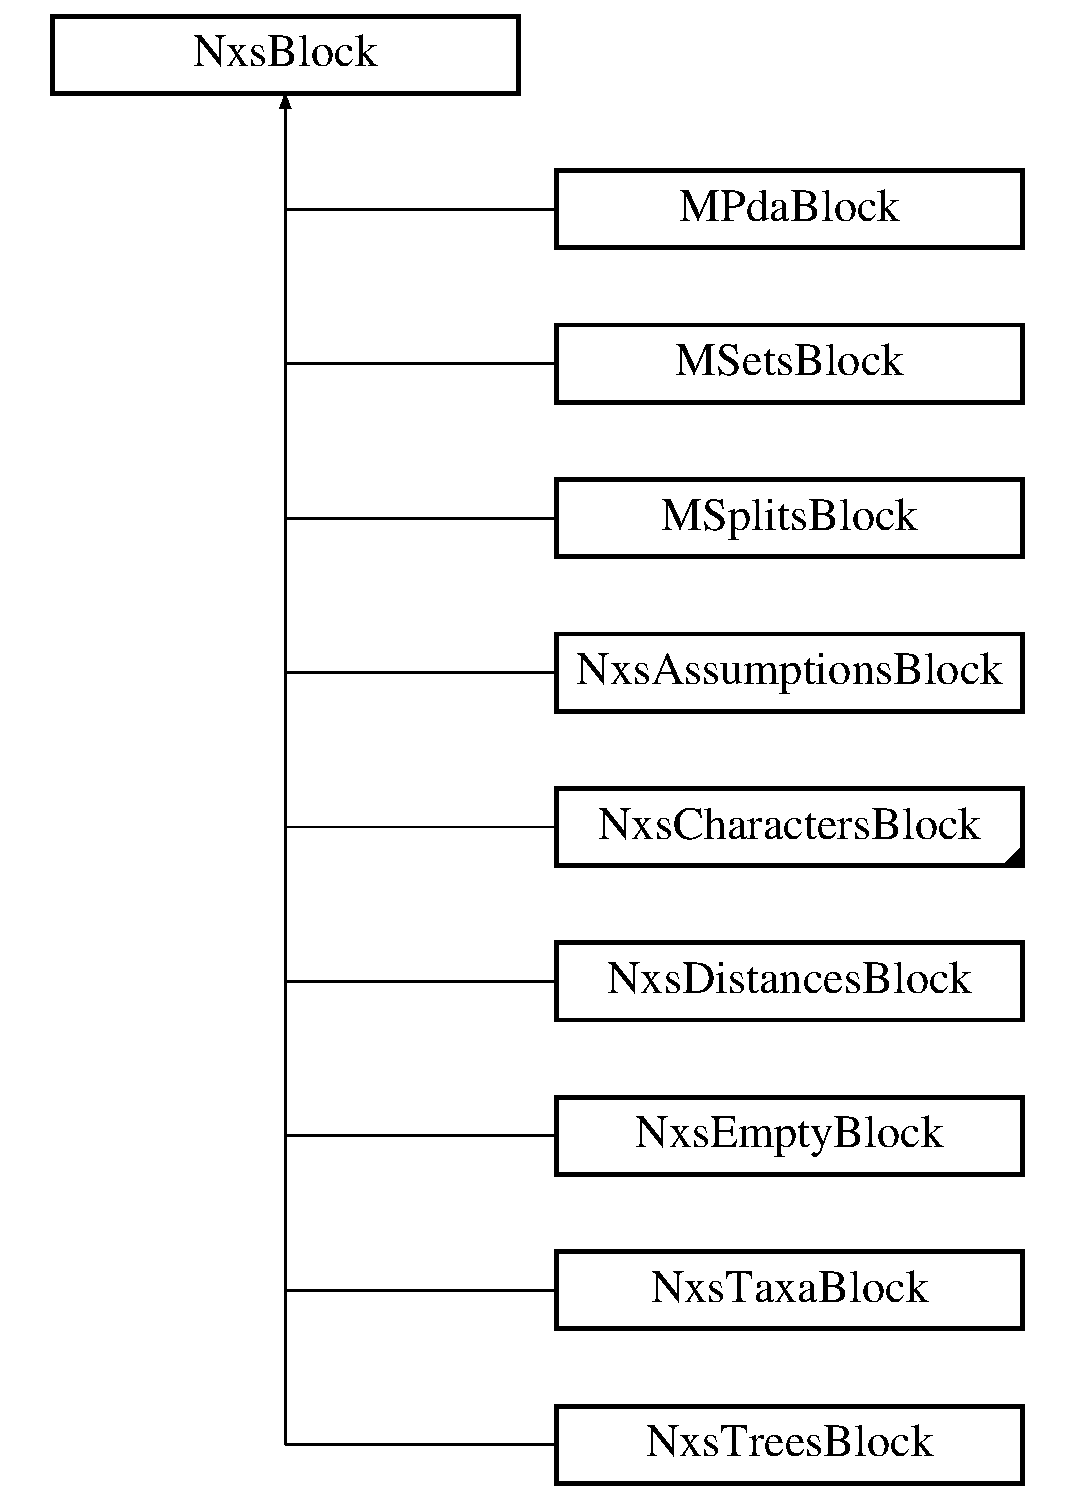
\includegraphics[height=10cm]{classNxsBlock}
\end{center}
\end{figure}
\subsection*{Public Member Functions}
\begin{DoxyCompactItemize}
\item 
\hypertarget{classNxsBlock_ade0e632784669a14df73fa0dc927d6b2}{
void {\bfseries SetNexus} (\hyperlink{classNxsReader}{NxsReader} $\ast$nxsptr)}
\label{classNxsBlock_ade0e632784669a14df73fa0dc927d6b2}

\item 
\hypertarget{classNxsBlock_a69f8ef50e0b6ab9a967b02f35d226e4e}{
\hyperlink{classNxsString}{NxsString} {\bfseries GetID} ()}
\label{classNxsBlock_a69f8ef50e0b6ab9a967b02f35d226e4e}

\item 
\hypertarget{classNxsBlock_adb227d7b480839feaf8f352993c746b4}{
bool {\bfseries IsEmpty} ()}
\label{classNxsBlock_adb227d7b480839feaf8f352993c746b4}

\item 
\hypertarget{classNxsBlock_ae3236495862428eb16ffe8fa841fd76a}{
void {\bfseries Enable} ()}
\label{classNxsBlock_ae3236495862428eb16ffe8fa841fd76a}

\item 
\hypertarget{classNxsBlock_a08fd00d328cba58ead5a98f8edd39f14}{
void {\bfseries Disable} ()}
\label{classNxsBlock_a08fd00d328cba58ead5a98f8edd39f14}

\item 
\hypertarget{classNxsBlock_aad4bd8800e59e1504036525c945aea55}{
bool {\bfseries IsEnabled} ()}
\label{classNxsBlock_aad4bd8800e59e1504036525c945aea55}

\item 
\hypertarget{classNxsBlock_a8e41dfbbba26e86d841ca917ea0cdfcd}{
bool {\bfseries IsUserSupplied} ()}
\label{classNxsBlock_a8e41dfbbba26e86d841ca917ea0cdfcd}

\item 
\hypertarget{classNxsBlock_ae7eb26a193ae8f65017427e83a69de0e}{
virtual unsigned {\bfseries CharLabelToNumber} (\hyperlink{classNxsString}{NxsString} s)}
\label{classNxsBlock_ae7eb26a193ae8f65017427e83a69de0e}

\item 
\hypertarget{classNxsBlock_a22fe174afbb5f5a97c3eb386ea43c8c8}{
virtual unsigned {\bfseries TaxonLabelToNumber} (\hyperlink{classNxsString}{NxsString} s)}
\label{classNxsBlock_a22fe174afbb5f5a97c3eb386ea43c8c8}

\item 
\hypertarget{classNxsBlock_ad369f29d49db5f6bc0d9603571813cb5}{
virtual void {\bfseries SkippingCommand} (\hyperlink{classNxsString}{NxsString} commandName)}
\label{classNxsBlock_ad369f29d49db5f6bc0d9603571813cb5}

\item 
\hypertarget{classNxsBlock_a7c88492f921b9952381c57c59233a04f}{
virtual void {\bfseries Report} (std::ostream \&out)}
\label{classNxsBlock_a7c88492f921b9952381c57c59233a04f}

\item 
\hypertarget{classNxsBlock_a3642d732dd82298ef2f35a7b83b97719}{
virtual void {\bfseries Reset} ()}
\label{classNxsBlock_a3642d732dd82298ef2f35a7b83b97719}

\end{DoxyCompactItemize}
\subsection*{Public Attributes}
\begin{DoxyCompactItemize}
\item 
\hypertarget{classNxsBlock_a8d85c9a7d0e2958b5531a9b734bdc1ea}{
\hyperlink{classNxsString}{NxsString} {\bfseries errormsg}}
\label{classNxsBlock_a8d85c9a7d0e2958b5531a9b734bdc1ea}

\end{DoxyCompactItemize}
\subsection*{Protected Member Functions}
\begin{DoxyCompactItemize}
\item 
\hypertarget{classNxsBlock_a3b7a229312d9182c6a7a3823d0e46a69}{
virtual void {\bfseries Read} (\hyperlink{classNxsToken}{NxsToken} \&token)}
\label{classNxsBlock_a3b7a229312d9182c6a7a3823d0e46a69}

\end{DoxyCompactItemize}
\subsection*{Protected Attributes}
\begin{DoxyCompactItemize}
\item 
\hypertarget{classNxsBlock_a3838d36624b7c4dbe47abfc558804f24}{
bool {\bfseries isEmpty}}
\label{classNxsBlock_a3838d36624b7c4dbe47abfc558804f24}

\item 
\hypertarget{classNxsBlock_a05a921edcd6bafc355b0c80352ada90d}{
bool {\bfseries isEnabled}}
\label{classNxsBlock_a05a921edcd6bafc355b0c80352ada90d}

\item 
\hypertarget{classNxsBlock_a6d7a0fdf8299bdaeca506f9c679fe804}{
bool {\bfseries isUserSupplied}}
\label{classNxsBlock_a6d7a0fdf8299bdaeca506f9c679fe804}

\item 
\hypertarget{classNxsBlock_a19738e5181f077f44a194d1841abc897}{
\hyperlink{classNxsReader}{NxsReader} $\ast$ {\bfseries nexus}}
\label{classNxsBlock_a19738e5181f077f44a194d1841abc897}

\item 
\hypertarget{classNxsBlock_a7af6b491ff4bbc4430489843268a5520}{
\hyperlink{classNxsBlock}{NxsBlock} $\ast$ {\bfseries next}}
\label{classNxsBlock_a7af6b491ff4bbc4430489843268a5520}

\item 
\hypertarget{classNxsBlock_a5adb993ee6e0e71448e5c51424ef30cb}{
\hyperlink{classNxsString}{NxsString} {\bfseries id}}
\label{classNxsBlock_a5adb993ee6e0e71448e5c51424ef30cb}

\end{DoxyCompactItemize}
\subsection*{Friends}
\begin{DoxyCompactItemize}
\item 
\hypertarget{classNxsBlock_a52410e92e5139842228caeaf0ac8dcc1}{
class \hyperlink{classNxsBlock_a52410e92e5139842228caeaf0ac8dcc1}{NxsReader}}
\label{classNxsBlock_a52410e92e5139842228caeaf0ac8dcc1}

\end{DoxyCompactItemize}


The documentation for this class was generated from the following files:\begin{DoxyCompactItemize}
\item 
src/ncl/nxsblock.h\item 
src/ncl/nxsblock.cpp\end{DoxyCompactItemize}

\hypertarget{classNxsCharactersBlock}{
\section{NxsCharactersBlock Class Reference}
\label{classNxsCharactersBlock}\index{NxsCharactersBlock@{NxsCharactersBlock}}
}
Inheritance diagram for NxsCharactersBlock::\begin{figure}[H]
\begin{center}
\leavevmode
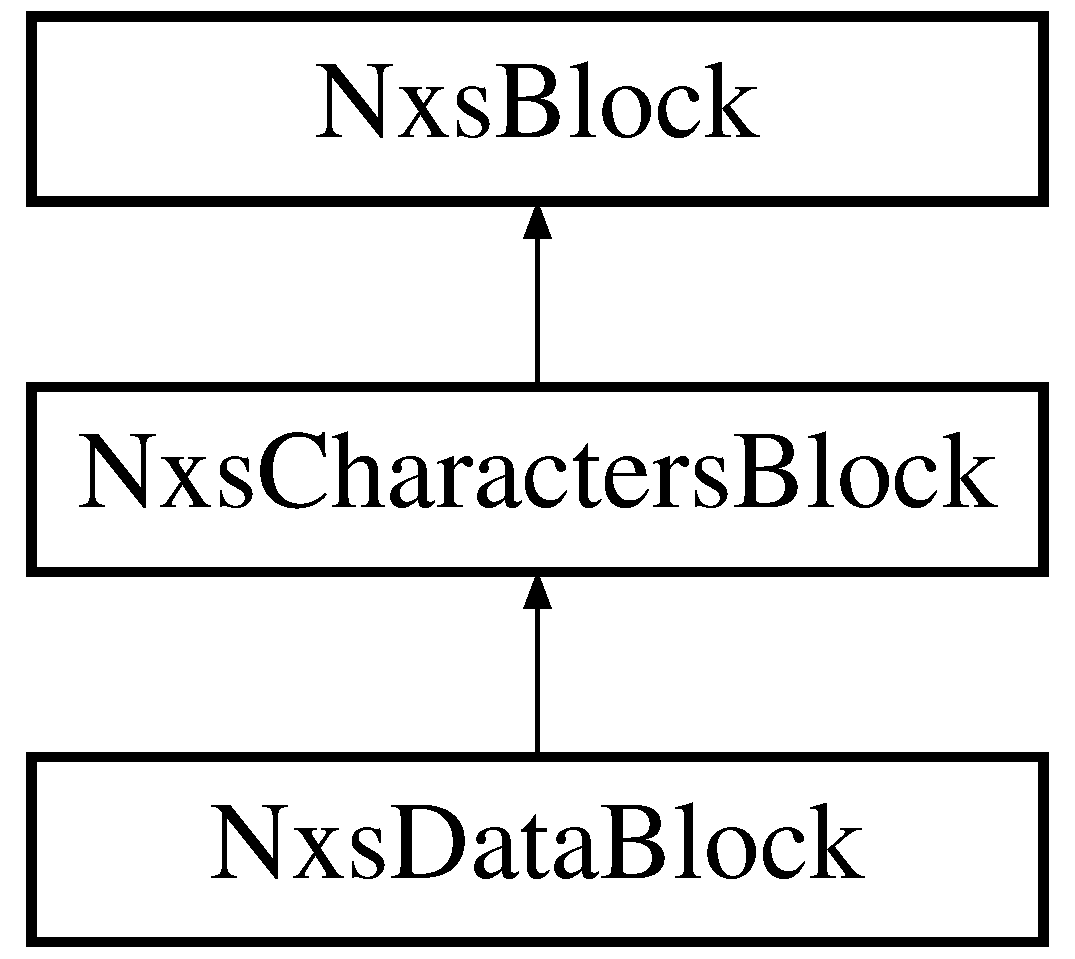
\includegraphics[height=3cm]{classNxsCharactersBlock}
\end{center}
\end{figure}
\subsection*{Public Types}
\begin{DoxyCompactItemize}
\item 
enum {\bfseries DataTypesEnum} \{ \par
{\bfseries standard} =  1, 
{\bfseries dna}, 
{\bfseries rna}, 
{\bfseries nucleotide}, 
\par
{\bfseries protein}, 
{\bfseries continuous}
 \}
\end{DoxyCompactItemize}
\subsection*{Public Member Functions}
\begin{DoxyCompactItemize}
\item 
\hypertarget{classNxsCharactersBlock_a8725c329790b33cdcf52c6aa1ee30b19}{
{\bfseries NxsCharactersBlock} (\hyperlink{classNxsTaxaBlock}{NxsTaxaBlock} $\ast$tb, \hyperlink{classNxsAssumptionsBlock}{NxsAssumptionsBlock} $\ast$ab)}
\label{classNxsCharactersBlock_a8725c329790b33cdcf52c6aa1ee30b19}

\item 
\hypertarget{classNxsCharactersBlock_ab8954865f54fb384cb13c299bd19b407}{
unsigned {\bfseries ApplyDelset} (NxsUnsignedSet \&delset)}
\label{classNxsCharactersBlock_ab8954865f54fb384cb13c299bd19b407}

\item 
\hypertarget{classNxsCharactersBlock_ae724d86e3ec64f4ee56962e69eabdb0b}{
unsigned {\bfseries ApplyExset} (NxsUnsignedSet \&exset)}
\label{classNxsCharactersBlock_ae724d86e3ec64f4ee56962e69eabdb0b}

\item 
\hypertarget{classNxsCharactersBlock_a39d83d6ddebf1b5abeda386812577d04}{
unsigned {\bfseries ApplyIncludeset} (NxsUnsignedSet \&inset)}
\label{classNxsCharactersBlock_a39d83d6ddebf1b5abeda386812577d04}

\item 
\hypertarget{classNxsCharactersBlock_a4ad02c2fc15ecb81f391f1ac27163de8}{
unsigned {\bfseries ApplyRestoreset} (NxsUnsignedSet \&restoreset)}
\label{classNxsCharactersBlock_a4ad02c2fc15ecb81f391f1ac27163de8}

\item 
\hypertarget{classNxsCharactersBlock_ad4b8b10e9e3367fa1ecac7a14266f3a8}{
unsigned {\bfseries GetCharPos} (unsigned origCharIndex)}
\label{classNxsCharactersBlock_ad4b8b10e9e3367fa1ecac7a14266f3a8}

\item 
\hypertarget{classNxsCharactersBlock_ae8ebb5ab6fb300779b5a67b2259a92db}{
unsigned {\bfseries GetTaxPos} (unsigned origTaxonIndex)}
\label{classNxsCharactersBlock_ae8ebb5ab6fb300779b5a67b2259a92db}

\item 
\hypertarget{classNxsCharactersBlock_a450d8f31ed9662e1930aac87eb61d8aa}{
unsigned {\bfseries GetDataType} ()}
\label{classNxsCharactersBlock_a450d8f31ed9662e1930aac87eb61d8aa}

\item 
\hypertarget{classNxsCharactersBlock_a681a9a39ad83766172e793139625029d}{
int {\bfseries GetInternalRepresentation} (unsigned i, unsigned j, unsigned k=0)}
\label{classNxsCharactersBlock_a681a9a39ad83766172e793139625029d}

\item 
\hypertarget{classNxsCharactersBlock_af86976f48a20f5070614d5bba79f5dd8}{
unsigned {\bfseries GetNTax} ()}
\label{classNxsCharactersBlock_af86976f48a20f5070614d5bba79f5dd8}

\item 
\hypertarget{classNxsCharactersBlock_a31fd31b367f9ea2ba68befafd375d098}{
unsigned {\bfseries GetNChar} ()}
\label{classNxsCharactersBlock_a31fd31b367f9ea2ba68befafd375d098}

\item 
\hypertarget{classNxsCharactersBlock_a68ae4020e94ccc851518bf1b75fee6db}{
unsigned {\bfseries GetNCharTotal} ()}
\label{classNxsCharactersBlock_a68ae4020e94ccc851518bf1b75fee6db}

\item 
\hypertarget{classNxsCharactersBlock_a201539150be60777b242bd51950970a9}{
unsigned {\bfseries GetNTaxTotal} ()}
\label{classNxsCharactersBlock_a201539150be60777b242bd51950970a9}

\item 
\hypertarget{classNxsCharactersBlock_a937d67e5d8dbacfb254ab558c7fe40fc}{
unsigned {\bfseries GetNumActiveChar} ()}
\label{classNxsCharactersBlock_a937d67e5d8dbacfb254ab558c7fe40fc}

\item 
\hypertarget{classNxsCharactersBlock_adcaf9c88dae34c0dc55a34d7c5c87bd7}{
unsigned {\bfseries GetNumActiveTaxa} ()}
\label{classNxsCharactersBlock_adcaf9c88dae34c0dc55a34d7c5c87bd7}

\item 
\hypertarget{classNxsCharactersBlock_a2487dd4245fe27bdd2875b28e220cb53}{
unsigned {\bfseries GetNumEliminated} ()}
\label{classNxsCharactersBlock_a2487dd4245fe27bdd2875b28e220cb53}

\item 
\hypertarget{classNxsCharactersBlock_a82168b018dec9309602c792d2186d2b9}{
unsigned {\bfseries GetNumEquates} ()}
\label{classNxsCharactersBlock_a82168b018dec9309602c792d2186d2b9}

\item 
\hypertarget{classNxsCharactersBlock_ad61b58c4ba502c3575e6e14dcfe07a77}{
unsigned {\bfseries GetNumMatrixCols} ()}
\label{classNxsCharactersBlock_ad61b58c4ba502c3575e6e14dcfe07a77}

\item 
\hypertarget{classNxsCharactersBlock_a74ebd4179a89e6c378fd4b5297ad4ebf}{
unsigned {\bfseries GetNumMatrixRows} ()}
\label{classNxsCharactersBlock_a74ebd4179a89e6c378fd4b5297ad4ebf}

\item 
\hypertarget{classNxsCharactersBlock_ad20d075197ab074d653d01fe8b073289}{
unsigned {\bfseries GetNumStates} (unsigned i, unsigned j)}
\label{classNxsCharactersBlock_ad20d075197ab074d653d01fe8b073289}

\item 
\hypertarget{classNxsCharactersBlock_a5ba82311067498a6fd9dcdb15850a617}{
unsigned {\bfseries GetOrigCharIndex} (unsigned j)}
\label{classNxsCharactersBlock_a5ba82311067498a6fd9dcdb15850a617}

\item 
\hypertarget{classNxsCharactersBlock_ad36d67a9d545e2f92ff11632f366a181}{
unsigned {\bfseries GetOrigCharNumber} (unsigned j)}
\label{classNxsCharactersBlock_ad36d67a9d545e2f92ff11632f366a181}

\item 
\hypertarget{classNxsCharactersBlock_a69cfbe6acdf4bfc6f08c0aa976aadaf3}{
unsigned {\bfseries GetOrigTaxonIndex} (unsigned j)}
\label{classNxsCharactersBlock_a69cfbe6acdf4bfc6f08c0aa976aadaf3}

\item 
\hypertarget{classNxsCharactersBlock_a304faaeb4e1e4288e0b1129e6a92c3d9}{
unsigned {\bfseries GetOrigTaxonNumber} (unsigned j)}
\label{classNxsCharactersBlock_a304faaeb4e1e4288e0b1129e6a92c3d9}

\item 
\hypertarget{classNxsCharactersBlock_a4b8703839c71602a102aed13c6633519}{
char {\bfseries GetGapSymbol} ()}
\label{classNxsCharactersBlock_a4b8703839c71602a102aed13c6633519}

\item 
\hypertarget{classNxsCharactersBlock_a50da85f7069ada52108f0b823c4560f4}{
char {\bfseries GetMatchcharSymbol} ()}
\label{classNxsCharactersBlock_a50da85f7069ada52108f0b823c4560f4}

\item 
\hypertarget{classNxsCharactersBlock_ae8bd3c4778a0e9932580fb144c11afea}{
char {\bfseries GetMissingSymbol} ()}
\label{classNxsCharactersBlock_ae8bd3c4778a0e9932580fb144c11afea}

\item 
\hypertarget{classNxsCharactersBlock_a17e72cc245c600ee8722fb69f751874e}{
bool {\bfseries IsGapState} (unsigned i, unsigned j)}
\label{classNxsCharactersBlock_a17e72cc245c600ee8722fb69f751874e}

\item 
\hypertarget{classNxsCharactersBlock_a358ef8de2a1b95187386708e4fd33990}{
bool {\bfseries IsInterleave} ()}
\label{classNxsCharactersBlock_a358ef8de2a1b95187386708e4fd33990}

\item 
\hypertarget{classNxsCharactersBlock_a3d59bc7867cb9843d776f6c6d9ee9dd2}{
bool {\bfseries IsLabels} ()}
\label{classNxsCharactersBlock_a3d59bc7867cb9843d776f6c6d9ee9dd2}

\item 
\hypertarget{classNxsCharactersBlock_a31b36c09144f155727cd05abe6a433a9}{
bool {\bfseries IsMissingState} (unsigned i, unsigned j)}
\label{classNxsCharactersBlock_a31b36c09144f155727cd05abe6a433a9}

\item 
\hypertarget{classNxsCharactersBlock_acd4f1bc9b1752d7053ae21d3ce235fa3}{
bool {\bfseries IsPolymorphic} (unsigned i, unsigned j)}
\label{classNxsCharactersBlock_acd4f1bc9b1752d7053ae21d3ce235fa3}

\item 
\hypertarget{classNxsCharactersBlock_ad41a9b80dbddf86530202c617548bde6}{
bool {\bfseries IsRespectCase} ()}
\label{classNxsCharactersBlock_ad41a9b80dbddf86530202c617548bde6}

\item 
\hypertarget{classNxsCharactersBlock_acbf05dc8273866d8fe7c23045d983758}{
bool {\bfseries IsTokens} ()}
\label{classNxsCharactersBlock_acbf05dc8273866d8fe7c23045d983758}

\item 
\hypertarget{classNxsCharactersBlock_a12980167f9e6a555ffa6cb466cadbb6f}{
bool {\bfseries IsTranspose} ()}
\label{classNxsCharactersBlock_a12980167f9e6a555ffa6cb466cadbb6f}

\item 
\hypertarget{classNxsCharactersBlock_a4d585738466acb117f62235a7d74f0c4}{
bool {\bfseries IsEliminated} (unsigned origCharIndex)}
\label{classNxsCharactersBlock_a4d585738466acb117f62235a7d74f0c4}

\item 
\hypertarget{classNxsCharactersBlock_a95c89bcff05d6d3718c39a74e859369f}{
void {\bfseries Consume} (\hyperlink{classNxsCharactersBlock}{NxsCharactersBlock} \&other)}
\label{classNxsCharactersBlock_a95c89bcff05d6d3718c39a74e859369f}

\item 
\hypertarget{classNxsCharactersBlock_a5c12fb5d3295cce9292839d9fe774e1b}{
void {\bfseries ExcludeCharacter} (unsigned i)}
\label{classNxsCharactersBlock_a5c12fb5d3295cce9292839d9fe774e1b}

\item 
\hypertarget{classNxsCharactersBlock_a77cae32fe241edccb568c974f84f4d6e}{
void {\bfseries IncludeCharacter} (unsigned i)}
\label{classNxsCharactersBlock_a77cae32fe241edccb568c974f84f4d6e}

\item 
\hypertarget{classNxsCharactersBlock_a25aae5cc0a427e49584f3a9413ac3d08}{
bool {\bfseries IsActiveChar} (unsigned j)}
\label{classNxsCharactersBlock_a25aae5cc0a427e49584f3a9413ac3d08}

\item 
\hypertarget{classNxsCharactersBlock_afa5db060aaac010e1715f4e4f4e0c280}{
bool {\bfseries IsExcluded} (unsigned j)}
\label{classNxsCharactersBlock_afa5db060aaac010e1715f4e4f4e0c280}

\item 
\hypertarget{classNxsCharactersBlock_a9b5e518a17c0faf5fc74e08bef824747}{
void {\bfseries DeleteTaxon} (unsigned i)}
\label{classNxsCharactersBlock_a9b5e518a17c0faf5fc74e08bef824747}

\item 
\hypertarget{classNxsCharactersBlock_a9d70d4f161d881b06c6321a7a6c0d18c}{
void {\bfseries RestoreTaxon} (unsigned i)}
\label{classNxsCharactersBlock_a9d70d4f161d881b06c6321a7a6c0d18c}

\item 
\hypertarget{classNxsCharactersBlock_afb7e89237e90c6012fb43144ce676f2a}{
bool {\bfseries IsActiveTaxon} (unsigned i)}
\label{classNxsCharactersBlock_afb7e89237e90c6012fb43144ce676f2a}

\item 
\hypertarget{classNxsCharactersBlock_abaf10f1fcc54eff6db1f9feba225b31a}{
bool {\bfseries IsDeleted} (unsigned i)}
\label{classNxsCharactersBlock_abaf10f1fcc54eff6db1f9feba225b31a}

\item 
\hypertarget{classNxsCharactersBlock_a3ec722e8713bac7824a4fda5de072722}{
void {\bfseries ShowStateLabels} (ostream \&out, unsigned i, unsigned c, unsigned first\_\-taxon=-\/1)}
\label{classNxsCharactersBlock_a3ec722e8713bac7824a4fda5de072722}

\item 
\hypertarget{classNxsCharactersBlock_a7331c7b7cd5bf5a3dfc43adf0efd4e40}{
unsigned {\bfseries GetStateSymbolIndex} (unsigned i, unsigned j, unsigned k=0)}
\label{classNxsCharactersBlock_a7331c7b7cd5bf5a3dfc43adf0efd4e40}

\item 
\hypertarget{classNxsCharactersBlock_a5109912828413e406a0884db25625923}{
char {\bfseries GetState} (unsigned i, unsigned j, unsigned k=0)}
\label{classNxsCharactersBlock_a5109912828413e406a0884db25625923}

\item 
\hypertarget{classNxsCharactersBlock_a43f0fb559f83dad0506074fde144fa1c}{
char $\ast$ {\bfseries GetSymbols} ()}
\label{classNxsCharactersBlock_a43f0fb559f83dad0506074fde144fa1c}

\item 
\hypertarget{classNxsCharactersBlock_ab396aa3b6513467319db9d4ec79b3491}{
bool $\ast$ {\bfseries GetActiveTaxonArray} ()}
\label{classNxsCharactersBlock_ab396aa3b6513467319db9d4ec79b3491}

\item 
\hypertarget{classNxsCharactersBlock_ae4053fcae2b3e2c4717d56a307ff43bc}{
bool $\ast$ {\bfseries GetActiveCharArray} ()}
\label{classNxsCharactersBlock_ae4053fcae2b3e2c4717d56a307ff43bc}

\item 
\hypertarget{classNxsCharactersBlock_a78a05d5817099b1ca757bf2f98d6eee4}{
\hyperlink{classNxsString}{NxsString} {\bfseries GetCharLabel} (unsigned i)}
\label{classNxsCharactersBlock_a78a05d5817099b1ca757bf2f98d6eee4}

\item 
\hypertarget{classNxsCharactersBlock_a97fb878930c0c923f5d5782784f9a30f}{
\hyperlink{classNxsString}{NxsString} {\bfseries GetStateLabel} (unsigned i, unsigned j)}
\label{classNxsCharactersBlock_a97fb878930c0c923f5d5782784f9a30f}

\item 
\hypertarget{classNxsCharactersBlock_a5e3fef4cb87159439657eeaa87915bca}{
\hyperlink{classNxsString}{NxsString} {\bfseries GetTaxonLabel} (unsigned i)}
\label{classNxsCharactersBlock_a5e3fef4cb87159439657eeaa87915bca}

\item 
\hypertarget{classNxsCharactersBlock_a8d74801e350fac497cfe131f42f69827}{
virtual unsigned {\bfseries CharLabelToNumber} (\hyperlink{classNxsString}{NxsString} s)}
\label{classNxsCharactersBlock_a8d74801e350fac497cfe131f42f69827}

\item 
\hypertarget{classNxsCharactersBlock_afbd900762109bd46339bf37f3996a04b}{
virtual unsigned {\bfseries TaxonLabelToNumber} (\hyperlink{classNxsString}{NxsString} s)}
\label{classNxsCharactersBlock_afbd900762109bd46339bf37f3996a04b}

\item 
\hypertarget{classNxsCharactersBlock_a5f69b7cf427afe4b9000bf1c574fc1e5}{
virtual unsigned {\bfseries GetMaxObsNumStates} ()}
\label{classNxsCharactersBlock_a5f69b7cf427afe4b9000bf1c574fc1e5}

\item 
\hypertarget{classNxsCharactersBlock_abcb7a058864974a71803856ac008f76a}{
virtual unsigned {\bfseries GetObsNumStates} (unsigned j)}
\label{classNxsCharactersBlock_abcb7a058864974a71803856ac008f76a}

\item 
\hypertarget{classNxsCharactersBlock_a6454d17f2bed1a5355f7b068362fbea0}{
virtual void {\bfseries DebugShowMatrix} (ostream \&out, bool use\_\-matchchar, const char $\ast$marginText=NULL)}
\label{classNxsCharactersBlock_a6454d17f2bed1a5355f7b068362fbea0}

\item 
\hypertarget{classNxsCharactersBlock_a13ed7f2a0dfbbdae5d62905232ccfe61}{
virtual void {\bfseries Report} (ostream \&out)}
\label{classNxsCharactersBlock_a13ed7f2a0dfbbdae5d62905232ccfe61}

\item 
\hypertarget{classNxsCharactersBlock_a2e479f3c7a744057e5ee3e653f9061e9}{
virtual void {\bfseries Reset} ()}
\label{classNxsCharactersBlock_a2e479f3c7a744057e5ee3e653f9061e9}

\end{DoxyCompactItemize}
\subsection*{Protected Member Functions}
\begin{DoxyCompactItemize}
\item 
\hypertarget{classNxsCharactersBlock_ac4e2040633ec934055c68229b7030129}{
void {\bfseries BuildCharPosArray} (bool check\_\-eliminated=false)}
\label{classNxsCharactersBlock_ac4e2040633ec934055c68229b7030129}

\item 
\hypertarget{classNxsCharactersBlock_adda12e700129a5adbcb62d04dfb5aea4}{
bool {\bfseries IsInSymbols} (char ch)}
\label{classNxsCharactersBlock_adda12e700129a5adbcb62d04dfb5aea4}

\item 
\hypertarget{classNxsCharactersBlock_a687f6d028e959d04e8662251b1946514}{
void {\bfseries HandleCharlabels} (\hyperlink{classNxsToken}{NxsToken} \&token)}
\label{classNxsCharactersBlock_a687f6d028e959d04e8662251b1946514}

\item 
\hypertarget{classNxsCharactersBlock_a28830ac9b39ade49fefafb2e7ba33a16}{
void {\bfseries HandleCharstatelabels} (\hyperlink{classNxsToken}{NxsToken} \&token)}
\label{classNxsCharactersBlock_a28830ac9b39ade49fefafb2e7ba33a16}

\item 
\hypertarget{classNxsCharactersBlock_a2403d3b7e8c91566a2bb39dc7807e33e}{
void {\bfseries HandleDimensions} (\hyperlink{classNxsToken}{NxsToken} \&token, \hyperlink{classNxsString}{NxsString} newtaxaLabel, \hyperlink{classNxsString}{NxsString} ntaxLabel, \hyperlink{classNxsString}{NxsString} ncharLabel)}
\label{classNxsCharactersBlock_a2403d3b7e8c91566a2bb39dc7807e33e}

\item 
\hypertarget{classNxsCharactersBlock_a051b9cfd99599fd8894c067274952d30}{
void {\bfseries HandleEliminate} (\hyperlink{classNxsToken}{NxsToken} \&token)}
\label{classNxsCharactersBlock_a051b9cfd99599fd8894c067274952d30}

\item 
\hypertarget{classNxsCharactersBlock_a635fe7add4fee21d8d40a3f50ab1d740}{
void {\bfseries HandleEndblock} (\hyperlink{classNxsToken}{NxsToken} \&token, \hyperlink{classNxsString}{NxsString} charToken)}
\label{classNxsCharactersBlock_a635fe7add4fee21d8d40a3f50ab1d740}

\item 
\hypertarget{classNxsCharactersBlock_a8fc039e274e43180293b6f0741f5486f}{
virtual void {\bfseries HandleFormat} (\hyperlink{classNxsToken}{NxsToken} \&token)}
\label{classNxsCharactersBlock_a8fc039e274e43180293b6f0741f5486f}

\item 
\hypertarget{classNxsCharactersBlock_ac3182cda60e8ecb7bf6fbef6abe187ee}{
virtual void {\bfseries HandleMatrix} (\hyperlink{classNxsToken}{NxsToken} \&token)}
\label{classNxsCharactersBlock_ac3182cda60e8ecb7bf6fbef6abe187ee}

\item 
\hypertarget{classNxsCharactersBlock_ab5a639cfe3cecacf98fbf21232507fd8}{
virtual bool {\bfseries HandleNextState} (\hyperlink{classNxsToken}{NxsToken} \&token, unsigned i, unsigned c)}
\label{classNxsCharactersBlock_ab5a639cfe3cecacf98fbf21232507fd8}

\item 
\hypertarget{classNxsCharactersBlock_afa4e2954e61ccdfaafda0609d294d729}{
virtual void {\bfseries HandleStdMatrix} (\hyperlink{classNxsToken}{NxsToken} \&token)}
\label{classNxsCharactersBlock_afa4e2954e61ccdfaafda0609d294d729}

\item 
\hypertarget{classNxsCharactersBlock_aa9ee838c740babd226c917f716a281da}{
virtual unsigned {\bfseries HandleTokenState} (\hyperlink{classNxsToken}{NxsToken} \&token, unsigned c)}
\label{classNxsCharactersBlock_aa9ee838c740babd226c917f716a281da}

\item 
\hypertarget{classNxsCharactersBlock_ad1e6cab805c606e17d5d57b2e5e36b50}{
virtual void {\bfseries HandleTransposedMatrix} (\hyperlink{classNxsToken}{NxsToken} \&token)}
\label{classNxsCharactersBlock_ad1e6cab805c606e17d5d57b2e5e36b50}

\item 
\hypertarget{classNxsCharactersBlock_af13ecbcad48d15bcade4eb44875644dd}{
virtual void {\bfseries Read} (\hyperlink{classNxsToken}{NxsToken} \&token)}
\label{classNxsCharactersBlock_af13ecbcad48d15bcade4eb44875644dd}

\item 
\hypertarget{classNxsCharactersBlock_a6b1936d89a877e42178d00543a322c02}{
unsigned {\bfseries PositionInSymbols} (char ch)}
\label{classNxsCharactersBlock_a6b1936d89a877e42178d00543a322c02}

\item 
\hypertarget{classNxsCharactersBlock_ae52c5cc8b8e1a8473be02c9a1ec63dfc}{
void {\bfseries HandleStatelabels} (\hyperlink{classNxsToken}{NxsToken} \&token)}
\label{classNxsCharactersBlock_ae52c5cc8b8e1a8473be02c9a1ec63dfc}

\item 
\hypertarget{classNxsCharactersBlock_a41f8b6956a6556e9cc5fd1d68bb834e7}{
void {\bfseries HandleTaxlabels} (\hyperlink{classNxsToken}{NxsToken} \&token)}
\label{classNxsCharactersBlock_a41f8b6956a6556e9cc5fd1d68bb834e7}

\item 
\hypertarget{classNxsCharactersBlock_a60329b2e678a91ca6cd46957093e6f56}{
void {\bfseries ResetSymbols} ()}
\label{classNxsCharactersBlock_a60329b2e678a91ca6cd46957093e6f56}

\item 
\hypertarget{classNxsCharactersBlock_aaeacb0381494d0b1d451135929874743}{
void {\bfseries ShowStates} (ostream \&out, unsigned i, unsigned j)}
\label{classNxsCharactersBlock_aaeacb0381494d0b1d451135929874743}

\item 
\hypertarget{classNxsCharactersBlock_a393ef5490c25965a1418115780afa3f8}{
void {\bfseries WriteStates} (\hyperlink{classNxsDiscreteDatum}{NxsDiscreteDatum} \&d, char $\ast$s, unsigned slen)}
\label{classNxsCharactersBlock_a393ef5490c25965a1418115780afa3f8}

\end{DoxyCompactItemize}
\subsection*{Protected Attributes}
\begin{DoxyCompactItemize}
\item 
\hypertarget{classNxsCharactersBlock_a568870c5d3b91dfda7a380818cf71089}{
\hyperlink{classNxsTaxaBlock}{NxsTaxaBlock} $\ast$ {\bfseries taxa}}
\label{classNxsCharactersBlock_a568870c5d3b91dfda7a380818cf71089}

\item 
\hypertarget{classNxsCharactersBlock_aafbff474ceaddb7e7ced8763f4f85671}{
\hyperlink{classNxsAssumptionsBlock}{NxsAssumptionsBlock} $\ast$ {\bfseries assumptionsBlock}}
\label{classNxsCharactersBlock_aafbff474ceaddb7e7ced8763f4f85671}

\item 
\hypertarget{classNxsCharactersBlock_a507131223ec9381eb038bdf4f72772c2}{
unsigned {\bfseries ntax}}
\label{classNxsCharactersBlock_a507131223ec9381eb038bdf4f72772c2}

\item 
\hypertarget{classNxsCharactersBlock_ac97ac41ab36654d1740566fd7e025ffa}{
unsigned {\bfseries ntaxTotal}}
\label{classNxsCharactersBlock_ac97ac41ab36654d1740566fd7e025ffa}

\item 
\hypertarget{classNxsCharactersBlock_a1900011b78247598ad421ee1387bc9ab}{
unsigned {\bfseries nchar}}
\label{classNxsCharactersBlock_a1900011b78247598ad421ee1387bc9ab}

\item 
\hypertarget{classNxsCharactersBlock_aac04ff11e093c6fda180123a570a5b25}{
unsigned {\bfseries ncharTotal}}
\label{classNxsCharactersBlock_aac04ff11e093c6fda180123a570a5b25}

\item 
\hypertarget{classNxsCharactersBlock_a1748d02f27126e3e333993855aaf6d0e}{
bool {\bfseries newtaxa}}
\label{classNxsCharactersBlock_a1748d02f27126e3e333993855aaf6d0e}

\item 
\hypertarget{classNxsCharactersBlock_a3ccd76d32f6e970022b115734e326248}{
bool {\bfseries newchar}}
\label{classNxsCharactersBlock_a3ccd76d32f6e970022b115734e326248}

\item 
\hypertarget{classNxsCharactersBlock_a0556d651c9f4878a738590cb45397c3e}{
bool {\bfseries formerly\_\-datablock}}
\label{classNxsCharactersBlock_a0556d651c9f4878a738590cb45397c3e}

\item 
\hypertarget{classNxsCharactersBlock_ae49a072b05aaeb6e935b0c9ec58546ec}{
bool {\bfseries respectingCase}}
\label{classNxsCharactersBlock_ae49a072b05aaeb6e935b0c9ec58546ec}

\item 
\hypertarget{classNxsCharactersBlock_adcd310904cc0a2a45b897ee24df14eea}{
bool {\bfseries transposing}}
\label{classNxsCharactersBlock_adcd310904cc0a2a45b897ee24df14eea}

\item 
\hypertarget{classNxsCharactersBlock_ac2ee7ac653d6c64103f5f1d22623a42e}{
bool {\bfseries interleaving}}
\label{classNxsCharactersBlock_ac2ee7ac653d6c64103f5f1d22623a42e}

\item 
\hypertarget{classNxsCharactersBlock_a6b68dcd93531ade9e737717d1a45289f}{
bool {\bfseries tokens}}
\label{classNxsCharactersBlock_a6b68dcd93531ade9e737717d1a45289f}

\item 
\hypertarget{classNxsCharactersBlock_a4425a48b9ee7b7430f9ce8830bddfe28}{
bool {\bfseries labels}}
\label{classNxsCharactersBlock_a4425a48b9ee7b7430f9ce8830bddfe28}

\item 
\hypertarget{classNxsCharactersBlock_a2c8e17d398815513fb162f3e08a5d3e0}{
char {\bfseries missing}}
\label{classNxsCharactersBlock_a2c8e17d398815513fb162f3e08a5d3e0}

\item 
\hypertarget{classNxsCharactersBlock_a6966bcd592fcce0ccce990fe9f9e7a99}{
char {\bfseries gap}}
\label{classNxsCharactersBlock_a6966bcd592fcce0ccce990fe9f9e7a99}

\item 
\hypertarget{classNxsCharactersBlock_a81b8b7578d0b364480e73cffcf6d72b8}{
char {\bfseries matchchar}}
\label{classNxsCharactersBlock_a81b8b7578d0b364480e73cffcf6d72b8}

\item 
\hypertarget{classNxsCharactersBlock_a09f5996b8d2feb6818465eb1db10e7fc}{
char $\ast$ {\bfseries symbols}}
\label{classNxsCharactersBlock_a09f5996b8d2feb6818465eb1db10e7fc}

\item 
\hypertarget{classNxsCharactersBlock_a2aa1fa00c24e601ce86ca4c5e69a73ef}{
NxsStringMap {\bfseries equates}}
\label{classNxsCharactersBlock_a2aa1fa00c24e601ce86ca4c5e69a73ef}

\item 
\hypertarget{classNxsCharactersBlock_a0d2aad02c54cced5273878a960e47557}{
\hyperlink{classNxsDiscreteMatrix}{NxsDiscreteMatrix} $\ast$ {\bfseries matrix}}
\label{classNxsCharactersBlock_a0d2aad02c54cced5273878a960e47557}

\item 
\hypertarget{classNxsCharactersBlock_afaf75137ef3e389566bf3334964998c8}{
unsigned $\ast$ {\bfseries charPos}}
\label{classNxsCharactersBlock_afaf75137ef3e389566bf3334964998c8}

\item 
\hypertarget{classNxsCharactersBlock_a0428a316fae8eeb8af293370ce604598}{
unsigned $\ast$ {\bfseries taxonPos}}
\label{classNxsCharactersBlock_a0428a316fae8eeb8af293370ce604598}

\item 
\hypertarget{classNxsCharactersBlock_a37dbaacd79e577d99901dbc01834a012}{
NxsUnsignedSet {\bfseries eliminated}}
\label{classNxsCharactersBlock_a37dbaacd79e577d99901dbc01834a012}

\item 
\hypertarget{classNxsCharactersBlock_a73590a6876462d6a897e7ab2a0177a62}{
bool $\ast$ {\bfseries activeChar}}
\label{classNxsCharactersBlock_a73590a6876462d6a897e7ab2a0177a62}

\item 
\hypertarget{classNxsCharactersBlock_a0dbee8381f8575b0436f61b032e12ffe}{
bool $\ast$ {\bfseries activeTaxon}}
\label{classNxsCharactersBlock_a0dbee8381f8575b0436f61b032e12ffe}

\item 
\hypertarget{classNxsCharactersBlock_a3f9e1f582590b4fe7ca35bc1fd5d96c7}{
NxsStringVector {\bfseries charLabels}}
\label{classNxsCharactersBlock_a3f9e1f582590b4fe7ca35bc1fd5d96c7}

\item 
\hypertarget{classNxsCharactersBlock_a6e73be6a91ea04e9b220d79de72f1f49}{
NxsStringVectorMap {\bfseries charStates}}
\label{classNxsCharactersBlock_a6e73be6a91ea04e9b220d79de72f1f49}

\end{DoxyCompactItemize}
\subsection*{Friends}
\begin{DoxyCompactItemize}
\item 
\hypertarget{classNxsCharactersBlock_a97ede2c71acd1e6aa5521164f8eaba1e}{
class \hyperlink{classNxsCharactersBlock_a97ede2c71acd1e6aa5521164f8eaba1e}{NxsAssumptionsBlock}}
\label{classNxsCharactersBlock_a97ede2c71acd1e6aa5521164f8eaba1e}

\end{DoxyCompactItemize}


The documentation for this class was generated from the following files:\begin{DoxyCompactItemize}
\item 
src/ncl/nxscharactersblock.h\item 
src/ncl/nxscharactersblock.cpp\end{DoxyCompactItemize}

\hypertarget{classNxsDataBlock}{
\section{NxsDataBlock Class Reference}
\label{classNxsDataBlock}\index{NxsDataBlock@{NxsDataBlock}}
}
Inheritance diagram for NxsDataBlock::\begin{figure}[H]
\begin{center}
\leavevmode
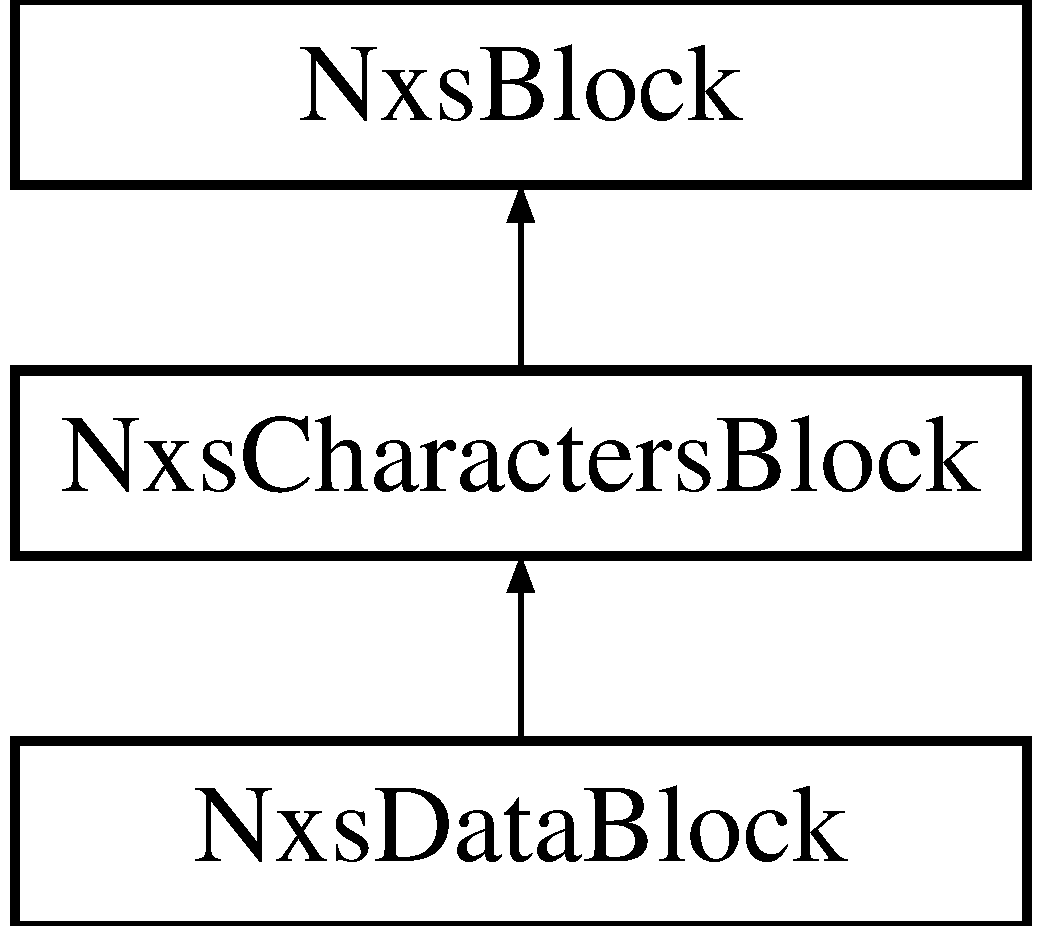
\includegraphics[height=3cm]{classNxsDataBlock}
\end{center}
\end{figure}
\subsection*{Public Member Functions}
\begin{DoxyCompactItemize}
\item 
\hypertarget{classNxsDataBlock_a48ab9ef4ea76a56b5eee04984362f5b7}{
{\bfseries NxsDataBlock} (\hyperlink{classNxsTaxaBlock}{NxsTaxaBlock} $\ast$tb, \hyperlink{classNxsAssumptionsBlock}{NxsAssumptionsBlock} $\ast$ab)}
\label{classNxsDataBlock_a48ab9ef4ea76a56b5eee04984362f5b7}

\item 
\hypertarget{classNxsDataBlock_a6362a21b1e29eab0db7c41792dc5c339}{
void {\bfseries TransferTo} (\hyperlink{classNxsCharactersBlock}{NxsCharactersBlock} \&charactersblock)}
\label{classNxsDataBlock_a6362a21b1e29eab0db7c41792dc5c339}

\item 
\hypertarget{classNxsDataBlock_afbb0d98c0a459bb77b318c314c80dff1}{
void {\bfseries Reset} ()}
\label{classNxsDataBlock_afbb0d98c0a459bb77b318c314c80dff1}

\end{DoxyCompactItemize}


The documentation for this class was generated from the following files:\begin{DoxyCompactItemize}
\item 
src/ncl/nxsdatablock.h\item 
src/ncl/nxsdatablock.cpp\end{DoxyCompactItemize}

\hypertarget{classNxsDiscreteDatum}{
\section{NxsDiscreteDatum Class Reference}
\label{classNxsDiscreteDatum}\index{NxsDiscreteDatum@{NxsDiscreteDatum}}
}
\subsection*{Public Member Functions}
\begin{DoxyCompactItemize}
\item 
\hypertarget{classNxsDiscreteDatum_a17f59c28cd4a83d49c152894d0548ceb}{
void {\bfseries CopyFrom} (const \hyperlink{classNxsDiscreteDatum}{NxsDiscreteDatum} \&other)}
\label{classNxsDiscreteDatum_a17f59c28cd4a83d49c152894d0548ceb}

\end{DoxyCompactItemize}
\subsection*{Friends}
\begin{DoxyCompactItemize}
\item 
\hypertarget{classNxsDiscreteDatum_a6c46ccb809a45095d7976b5d0e4466b2}{
class \hyperlink{classNxsDiscreteDatum_a6c46ccb809a45095d7976b5d0e4466b2}{NxsDiscreteMatrix}}
\label{classNxsDiscreteDatum_a6c46ccb809a45095d7976b5d0e4466b2}

\end{DoxyCompactItemize}


The documentation for this class was generated from the following files:\begin{DoxyCompactItemize}
\item 
src/ncl/nxsdiscretedatum.h\item 
src/ncl/nxsdiscretedatum.cpp\end{DoxyCompactItemize}

\hypertarget{classNxsDiscreteMatrix}{
\section{NxsDiscreteMatrix Class Reference}
\label{classNxsDiscreteMatrix}\index{NxsDiscreteMatrix@{NxsDiscreteMatrix}}
}
\subsection*{Public Member Functions}
\begin{DoxyCompactItemize}
\item 
\hypertarget{classNxsDiscreteMatrix_a537a120d005714989645805bb946a184}{
{\bfseries NxsDiscreteMatrix} (unsigned rows, unsigned cols)}
\label{classNxsDiscreteMatrix_a537a120d005714989645805bb946a184}

\item 
\hypertarget{classNxsDiscreteMatrix_a17c807f6229f13f93bd50b86726911be}{
void {\bfseries AddRows} (unsigned nAddRows)}
\label{classNxsDiscreteMatrix_a17c807f6229f13f93bd50b86726911be}

\item 
\hypertarget{classNxsDiscreteMatrix_aa748836bfeeaf4d91567539a5f06297b}{
void {\bfseries AddState} (unsigned i, unsigned j, unsigned value)}
\label{classNxsDiscreteMatrix_aa748836bfeeaf4d91567539a5f06297b}

\item 
\hypertarget{classNxsDiscreteMatrix_a9c833ce4c0f7770401014141bf0afad3}{
void {\bfseries CopyStatesFromFirstTaxon} (unsigned i, unsigned j)}
\label{classNxsDiscreteMatrix_a9c833ce4c0f7770401014141bf0afad3}

\item 
\hypertarget{classNxsDiscreteMatrix_a25211235186f83196e719a983673c5f1}{
void {\bfseries DebugSaveMatrix} (ostream \&out, unsigned colwidth=12)}
\label{classNxsDiscreteMatrix_a25211235186f83196e719a983673c5f1}

\item 
\hypertarget{classNxsDiscreteMatrix_aa521f18e6fc030122599c227644e9a4d}{
unsigned {\bfseries DuplicateRow} (unsigned row, unsigned count, unsigned startCol=0, unsigned endCol=UINT\_\-MAX)}
\label{classNxsDiscreteMatrix_aa521f18e6fc030122599c227644e9a4d}

\item 
\hypertarget{classNxsDiscreteMatrix_a89da8bcc568a9fa8b57a3c40453b8287}{
void {\bfseries Flush} ()}
\label{classNxsDiscreteMatrix_a89da8bcc568a9fa8b57a3c40453b8287}

\item 
\hypertarget{classNxsDiscreteMatrix_ada0b24e0f87ff41386c0947e51c340f1}{
unsigned {\bfseries GetState} (unsigned i, unsigned j, unsigned k=0)}
\label{classNxsDiscreteMatrix_ada0b24e0f87ff41386c0947e51c340f1}

\item 
\hypertarget{classNxsDiscreteMatrix_a5888814b520e5850ff6cf1ab11edc71d}{
unsigned {\bfseries GetNumStates} (unsigned i, unsigned j)}
\label{classNxsDiscreteMatrix_a5888814b520e5850ff6cf1ab11edc71d}

\item 
\hypertarget{classNxsDiscreteMatrix_a931d90b0bf6e031582b3d9c040e7ad6b}{
unsigned {\bfseries GetObsNumStates} (unsigned j)}
\label{classNxsDiscreteMatrix_a931d90b0bf6e031582b3d9c040e7ad6b}

\item 
\hypertarget{classNxsDiscreteMatrix_a1ff98ffcf216238b4dd43b74fe0f8941}{
bool {\bfseries IsGap} (unsigned i, unsigned j)}
\label{classNxsDiscreteMatrix_a1ff98ffcf216238b4dd43b74fe0f8941}

\item 
\hypertarget{classNxsDiscreteMatrix_a73adaad1c6b008aa44f2e4f181b6365a}{
bool {\bfseries IsMissing} (unsigned i, unsigned j)}
\label{classNxsDiscreteMatrix_a73adaad1c6b008aa44f2e4f181b6365a}

\item 
\hypertarget{classNxsDiscreteMatrix_a9614a45c41e6db08bd067999d26095a4}{
bool {\bfseries IsPolymorphic} (unsigned i, unsigned j)}
\label{classNxsDiscreteMatrix_a9614a45c41e6db08bd067999d26095a4}

\item 
\hypertarget{classNxsDiscreteMatrix_aa82127952da11e91b2c89b8937a52f64}{
void {\bfseries Reset} (unsigned rows, unsigned cols)}
\label{classNxsDiscreteMatrix_aa82127952da11e91b2c89b8937a52f64}

\item 
\hypertarget{classNxsDiscreteMatrix_a21162ff674ebeb3e2cb330ab0de6206e}{
void {\bfseries SetGap} (unsigned i, unsigned j)}
\label{classNxsDiscreteMatrix_a21162ff674ebeb3e2cb330ab0de6206e}

\item 
\hypertarget{classNxsDiscreteMatrix_a8afd5f10fb53529af048cd822fede5a9}{
void {\bfseries SetMissing} (unsigned i, unsigned j)}
\label{classNxsDiscreteMatrix_a8afd5f10fb53529af048cd822fede5a9}

\item 
\hypertarget{classNxsDiscreteMatrix_aef3c5167d49997c45c1913d1fd21bd11}{
void {\bfseries SetPolymorphic} (unsigned i, unsigned j, unsigned value=1)}
\label{classNxsDiscreteMatrix_aef3c5167d49997c45c1913d1fd21bd11}

\item 
\hypertarget{classNxsDiscreteMatrix_a7e7de3f9d25943e889917cbc989f2278}{
void {\bfseries SetState} (unsigned i, unsigned j, unsigned value)}
\label{classNxsDiscreteMatrix_a7e7de3f9d25943e889917cbc989f2278}

\end{DoxyCompactItemize}
\subsection*{Friends}
\begin{DoxyCompactItemize}
\item 
\hypertarget{classNxsDiscreteMatrix_ab9466d1b21f90b6fd961284f19c6e9d4}{
class \hyperlink{classNxsDiscreteMatrix_ab9466d1b21f90b6fd961284f19c6e9d4}{NxsCharactersBlock}}
\label{classNxsDiscreteMatrix_ab9466d1b21f90b6fd961284f19c6e9d4}

\item 
\hypertarget{classNxsDiscreteMatrix_ad9ba2bb6bba16b181df5d60f0c244681}{
class {\bfseries NxsAllelesBlock}}
\label{classNxsDiscreteMatrix_ad9ba2bb6bba16b181df5d60f0c244681}

\end{DoxyCompactItemize}


The documentation for this class was generated from the following files:\begin{DoxyCompactItemize}
\item 
src/ncl/nxsdiscretematrix.h\item 
src/ncl/nxsdiscretematrix.cpp\end{DoxyCompactItemize}

\hypertarget{classNxsDistanceDatum}{
\section{NxsDistanceDatum Class Reference}
\label{classNxsDistanceDatum}\index{NxsDistanceDatum@{NxsDistanceDatum}}
}
\subsection*{Friends}
\begin{DoxyCompactItemize}
\item 
\hypertarget{classNxsDistanceDatum_aa46e2fbd4a6264cf2f0f91035cdf6188}{
class \hyperlink{classNxsDistanceDatum_aa46e2fbd4a6264cf2f0f91035cdf6188}{NxsDistancesBlock}}
\label{classNxsDistanceDatum_aa46e2fbd4a6264cf2f0f91035cdf6188}

\end{DoxyCompactItemize}


The documentation for this class was generated from the following files:\begin{DoxyCompactItemize}
\item 
src/ncl/nxsdistancedatum.h\item 
src/ncl/nxsdistancedatum.cpp\end{DoxyCompactItemize}

\hypertarget{classNxsDistancesBlock}{
\section{NxsDistancesBlock Class Reference}
\label{classNxsDistancesBlock}\index{NxsDistancesBlock@{NxsDistancesBlock}}
}
Inheritance diagram for NxsDistancesBlock::\begin{figure}[H]
\begin{center}
\leavevmode
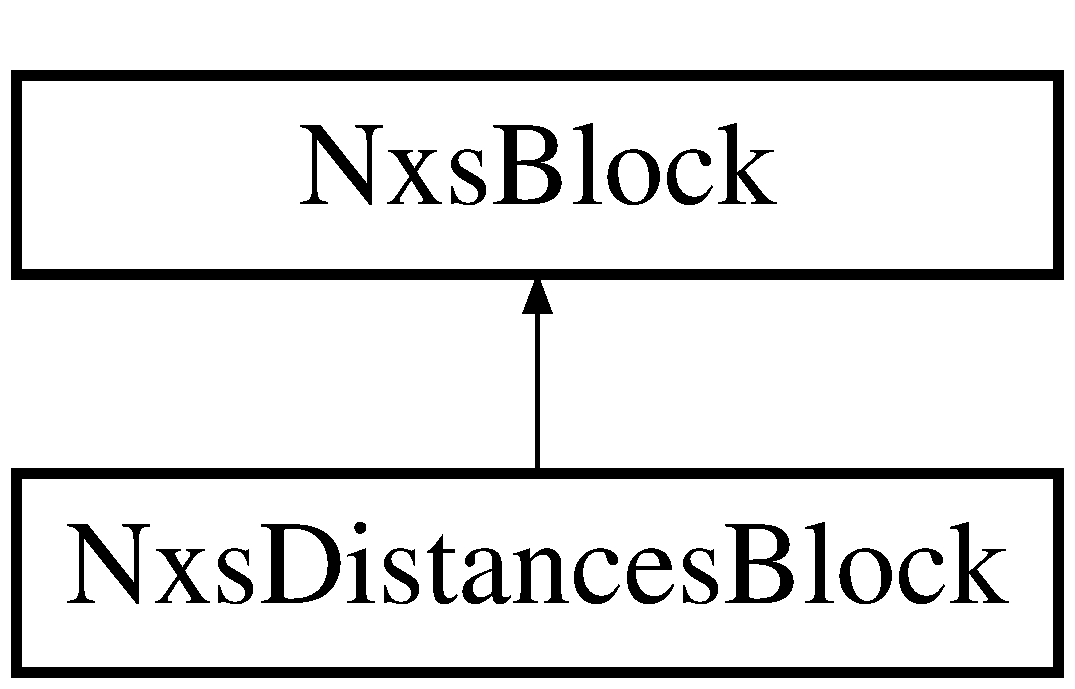
\includegraphics[height=2cm]{classNxsDistancesBlock}
\end{center}
\end{figure}
\subsection*{Public Types}
\begin{DoxyCompactItemize}
\item 
enum {\bfseries NxsDistancesBlockEnum} \{ {\bfseries upper} =  1, 
{\bfseries lower} =  2, 
{\bfseries both} =  3
 \}
\end{DoxyCompactItemize}
\subsection*{Public Member Functions}
\begin{DoxyCompactItemize}
\item 
\hypertarget{classNxsDistancesBlock_a0afb8eecb772d5def91a8ab45ef20564}{
{\bfseries NxsDistancesBlock} (\hyperlink{classNxsTaxaBlock}{NxsTaxaBlock} $\ast$t)}
\label{classNxsDistancesBlock_a0afb8eecb772d5def91a8ab45ef20564}

\item 
\hypertarget{classNxsDistancesBlock_ab98d07a76ea319334f4fa9154abe5f61}{
double {\bfseries GetDistance} (unsigned i, unsigned j)}
\label{classNxsDistancesBlock_ab98d07a76ea319334f4fa9154abe5f61}

\item 
\hypertarget{classNxsDistancesBlock_afe9b1dfa12825f9919b00cdaa41e156b}{
char {\bfseries GetMissingSymbol} ()}
\label{classNxsDistancesBlock_afe9b1dfa12825f9919b00cdaa41e156b}

\item 
\hypertarget{classNxsDistancesBlock_a8306a3d48d35bf3e1e1e8c23ffa096c2}{
unsigned {\bfseries GetNchar} ()}
\label{classNxsDistancesBlock_a8306a3d48d35bf3e1e1e8c23ffa096c2}

\item 
\hypertarget{classNxsDistancesBlock_a540edf63d4b225a488f36339411819f6}{
unsigned {\bfseries GetNtax} ()}
\label{classNxsDistancesBlock_a540edf63d4b225a488f36339411819f6}

\item 
\hypertarget{classNxsDistancesBlock_a40cc90a67e533b680fe9169ff25c70eb}{
unsigned {\bfseries GetTriangle} ()}
\label{classNxsDistancesBlock_a40cc90a67e533b680fe9169ff25c70eb}

\item 
\hypertarget{classNxsDistancesBlock_ab0284b8ebcd606ab989d11cc2351aa5d}{
bool {\bfseries IsRectangular} ()}
\label{classNxsDistancesBlock_ab0284b8ebcd606ab989d11cc2351aa5d}

\item 
\hypertarget{classNxsDistancesBlock_a2ff6b037d7deb7f088962df4f1df41f4}{
bool {\bfseries IsDiagonal} ()}
\label{classNxsDistancesBlock_a2ff6b037d7deb7f088962df4f1df41f4}

\item 
\hypertarget{classNxsDistancesBlock_a0c9bcad2e71262f51d2bc494d7981f9f}{
bool {\bfseries IsInterleave} ()}
\label{classNxsDistancesBlock_a0c9bcad2e71262f51d2bc494d7981f9f}

\item 
\hypertarget{classNxsDistancesBlock_af6063bb6cf45bee5590144adcab89673}{
bool {\bfseries IsLabels} ()}
\label{classNxsDistancesBlock_af6063bb6cf45bee5590144adcab89673}

\item 
\hypertarget{classNxsDistancesBlock_a454ff6c246f432f417f623fff68ca25d}{
bool {\bfseries IsLowerTriangular} ()}
\label{classNxsDistancesBlock_a454ff6c246f432f417f623fff68ca25d}

\item 
\hypertarget{classNxsDistancesBlock_aca14b29ff8132f68642f61c85bda31c1}{
bool {\bfseries IsMissing} (unsigned i, unsigned j)}
\label{classNxsDistancesBlock_aca14b29ff8132f68642f61c85bda31c1}

\item 
\hypertarget{classNxsDistancesBlock_a444b5d2109eb9d6120f7d8e00015b7ee}{
bool {\bfseries IsUpperTriangular} ()}
\label{classNxsDistancesBlock_a444b5d2109eb9d6120f7d8e00015b7ee}

\item 
\hypertarget{classNxsDistancesBlock_a2ae3df65eb0e820b0cd775ed250ee274}{
virtual void {\bfseries Report} (std::ostream \&out)}
\label{classNxsDistancesBlock_a2ae3df65eb0e820b0cd775ed250ee274}

\item 
\hypertarget{classNxsDistancesBlock_a67ad7aa8d41ab4c501b0955190eecdb4}{
virtual void {\bfseries Reset} ()}
\label{classNxsDistancesBlock_a67ad7aa8d41ab4c501b0955190eecdb4}

\item 
\hypertarget{classNxsDistancesBlock_abf60adc4c72d7cd3f9d618f5fc523dae}{
void {\bfseries SetDistance} (unsigned i, unsigned j, double d)}
\label{classNxsDistancesBlock_abf60adc4c72d7cd3f9d618f5fc523dae}

\item 
\hypertarget{classNxsDistancesBlock_adcdbab373c50bbb880fb1135ddd49318}{
void {\bfseries SetMissing} (unsigned i, unsigned j)}
\label{classNxsDistancesBlock_adcdbab373c50bbb880fb1135ddd49318}

\item 
\hypertarget{classNxsDistancesBlock_af6751142a49be625373bd1900aa6764a}{
void {\bfseries SetNchar} (unsigned i)}
\label{classNxsDistancesBlock_af6751142a49be625373bd1900aa6764a}

\end{DoxyCompactItemize}
\subsection*{Protected Member Functions}
\begin{DoxyCompactItemize}
\item 
\hypertarget{classNxsDistancesBlock_a2515878c3059a7289fddb1333bf3ab3a}{
void {\bfseries HandleDimensionsCommand} (\hyperlink{classNxsToken}{NxsToken} \&token)}
\label{classNxsDistancesBlock_a2515878c3059a7289fddb1333bf3ab3a}

\item 
\hypertarget{classNxsDistancesBlock_a935db45ad89e52f0b4b78f6b86c3d594}{
void {\bfseries HandleFormatCommand} (\hyperlink{classNxsToken}{NxsToken} \&token)}
\label{classNxsDistancesBlock_a935db45ad89e52f0b4b78f6b86c3d594}

\item 
\hypertarget{classNxsDistancesBlock_a34437a6e19eed81bfc1d1d5b6b7483d1}{
void {\bfseries HandleMatrixCommand} (\hyperlink{classNxsToken}{NxsToken} \&token)}
\label{classNxsDistancesBlock_a34437a6e19eed81bfc1d1d5b6b7483d1}

\item 
\hypertarget{classNxsDistancesBlock_a734b53f5d2d9ff8d406fb3d330972260}{
bool {\bfseries HandleNextPass} (\hyperlink{classNxsToken}{NxsToken} \&token, unsigned \&offset)}
\label{classNxsDistancesBlock_a734b53f5d2d9ff8d406fb3d330972260}

\item 
\hypertarget{classNxsDistancesBlock_ae23b77f2d2777f6728fa75e2d6bdc525}{
void {\bfseries HandleTaxlabelsCommand} (\hyperlink{classNxsToken}{NxsToken} \&token)}
\label{classNxsDistancesBlock_ae23b77f2d2777f6728fa75e2d6bdc525}

\item 
\hypertarget{classNxsDistancesBlock_ae1ba118f39196c10f788832f5abab6be}{
virtual void {\bfseries Read} (\hyperlink{classNxsToken}{NxsToken} \&token)}
\label{classNxsDistancesBlock_ae1ba118f39196c10f788832f5abab6be}

\end{DoxyCompactItemize}


The documentation for this class was generated from the following files:\begin{DoxyCompactItemize}
\item 
src/ncl/nxsdistancesblock.h\item 
src/ncl/nxsdistancesblock.cpp\end{DoxyCompactItemize}

\hypertarget{classNxsEmptyBlock}{
\section{NxsEmptyBlock Class Reference}
\label{classNxsEmptyBlock}\index{NxsEmptyBlock@{NxsEmptyBlock}}
}
Inheritance diagram for NxsEmptyBlock::\begin{figure}[H]
\begin{center}
\leavevmode
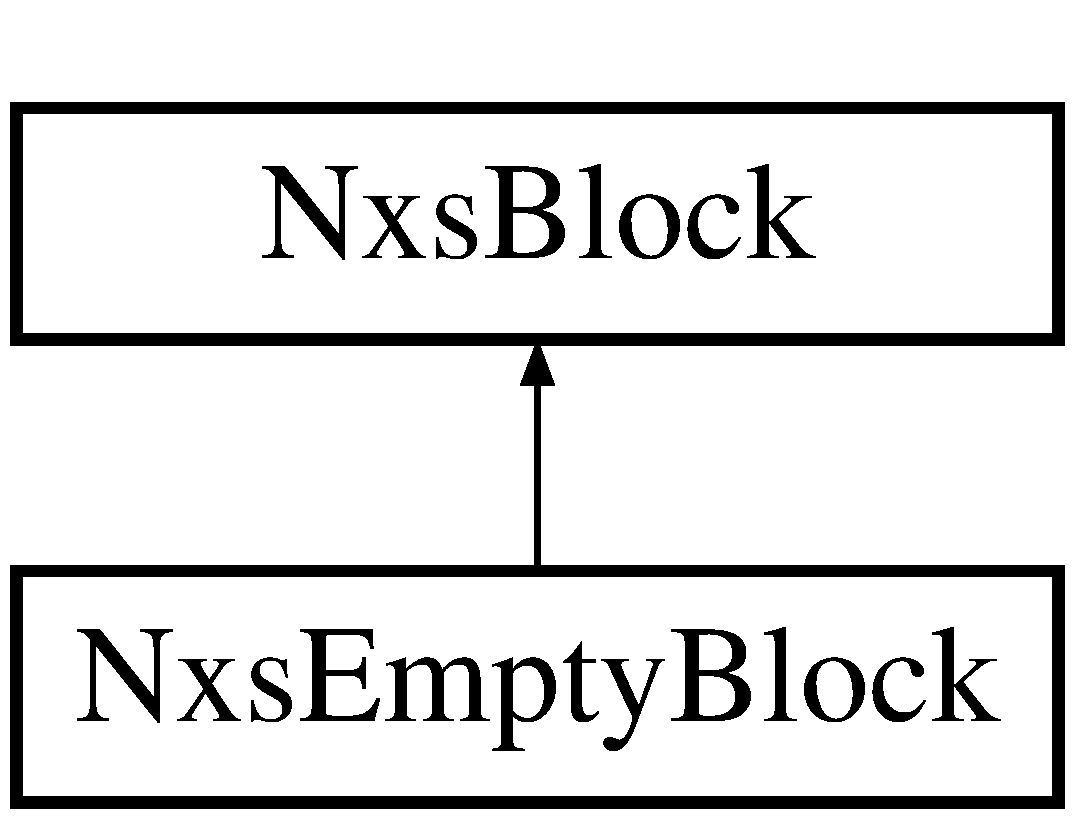
\includegraphics[height=2cm]{classNxsEmptyBlock}
\end{center}
\end{figure}
\subsection*{Public Member Functions}
\begin{DoxyCompactItemize}
\item 
\hypertarget{classNxsEmptyBlock_a9dc245da7055805dffd8ee400b2e24ae}{
virtual void {\bfseries Report} (ostream \&out)}
\label{classNxsEmptyBlock_a9dc245da7055805dffd8ee400b2e24ae}

\end{DoxyCompactItemize}
\subsection*{Protected Member Functions}
\begin{DoxyCompactItemize}
\item 
\hypertarget{classNxsEmptyBlock_a954ac92f354a0f8a35d95ba4b48ebfd5}{
void {\bfseries SkippingCommand} (\hyperlink{classNxsString}{NxsString} commandName)}
\label{classNxsEmptyBlock_a954ac92f354a0f8a35d95ba4b48ebfd5}

\item 
\hypertarget{classNxsEmptyBlock_a4e9244ea2c99002369d17ea29265890e}{
unsigned {\bfseries TaxonLabelToNumber} (\hyperlink{classNxsString}{NxsString} s)}
\label{classNxsEmptyBlock_a4e9244ea2c99002369d17ea29265890e}

\item 
\hypertarget{classNxsEmptyBlock_a3ba3c4cc2e8d54d23606b295a1f85ecf}{
unsigned {\bfseries CharLabelToNumber} (\hyperlink{classNxsString}{NxsString} s)}
\label{classNxsEmptyBlock_a3ba3c4cc2e8d54d23606b295a1f85ecf}

\item 
\hypertarget{classNxsEmptyBlock_ab55cc172c8c22ed1964e529745c67b70}{
void {\bfseries HandleEndblock} (\hyperlink{classNxsToken}{NxsToken} \&token)}
\label{classNxsEmptyBlock_ab55cc172c8c22ed1964e529745c67b70}

\item 
\hypertarget{classNxsEmptyBlock_ac41146480434ddb64d9471b34dbc779e}{
virtual void {\bfseries Read} (\hyperlink{classNxsToken}{NxsToken} \&token)}
\label{classNxsEmptyBlock_ac41146480434ddb64d9471b34dbc779e}

\item 
\hypertarget{classNxsEmptyBlock_a08f186cd2108bde98519a77e186fa2ab}{
virtual void {\bfseries Reset} ()}
\label{classNxsEmptyBlock_a08f186cd2108bde98519a77e186fa2ab}

\end{DoxyCompactItemize}


The documentation for this class was generated from the following files:\begin{DoxyCompactItemize}
\item 
src/ncl/nxsemptyblock.h\item 
src/ncl/nxsemptyblock.cpp\end{DoxyCompactItemize}

\hypertarget{classNxsException}{
\section{NxsException Class Reference}
\label{classNxsException}\index{NxsException@{NxsException}}
}
\subsection*{Public Member Functions}
\begin{DoxyCompactItemize}
\item 
\hypertarget{classNxsException_afbde84e7c1c8b01bd30fe1b1e3325d0e}{
{\bfseries NxsException} (\hyperlink{classNxsString}{NxsString} s, file\_\-pos fp=0, long fl=0L, long fc=0L)}
\label{classNxsException_afbde84e7c1c8b01bd30fe1b1e3325d0e}

\item 
\hypertarget{classNxsException_a3fc21e7072c996a1fa1a26413d3c19e7}{
{\bfseries NxsException} (const \hyperlink{classNxsString}{NxsString} \&s, const \hyperlink{classNxsToken}{NxsToken} \&t)}
\label{classNxsException_a3fc21e7072c996a1fa1a26413d3c19e7}

\end{DoxyCompactItemize}
\subsection*{Public Attributes}
\begin{DoxyCompactItemize}
\item 
\hypertarget{classNxsException_a7dba767f41b6231577b2f1d56b006f23}{
\hyperlink{classNxsString}{NxsString} {\bfseries msg}}
\label{classNxsException_a7dba767f41b6231577b2f1d56b006f23}

\item 
\hypertarget{classNxsException_a23a5c45f4ecf444ebdd0c9764df9b326}{
file\_\-pos {\bfseries pos}}
\label{classNxsException_a23a5c45f4ecf444ebdd0c9764df9b326}

\item 
\hypertarget{classNxsException_a4775b1e4ae814d024b1abec1afafeb2c}{
long {\bfseries line}}
\label{classNxsException_a4775b1e4ae814d024b1abec1afafeb2c}

\item 
\hypertarget{classNxsException_a73581aacb676bc6051733d4b53dd2fbc}{
long {\bfseries col}}
\label{classNxsException_a73581aacb676bc6051733d4b53dd2fbc}

\end{DoxyCompactItemize}


The documentation for this class was generated from the following files:\begin{DoxyCompactItemize}
\item 
src/ncl/nxsexception.h\item 
src/ncl/nxsexception.cpp\end{DoxyCompactItemize}

\hypertarget{classNxsReader}{
\section{NxsReader Class Reference}
\label{classNxsReader}\index{NxsReader@{NxsReader}}
}
Inheritance diagram for NxsReader::\begin{figure}[H]
\begin{center}
\leavevmode
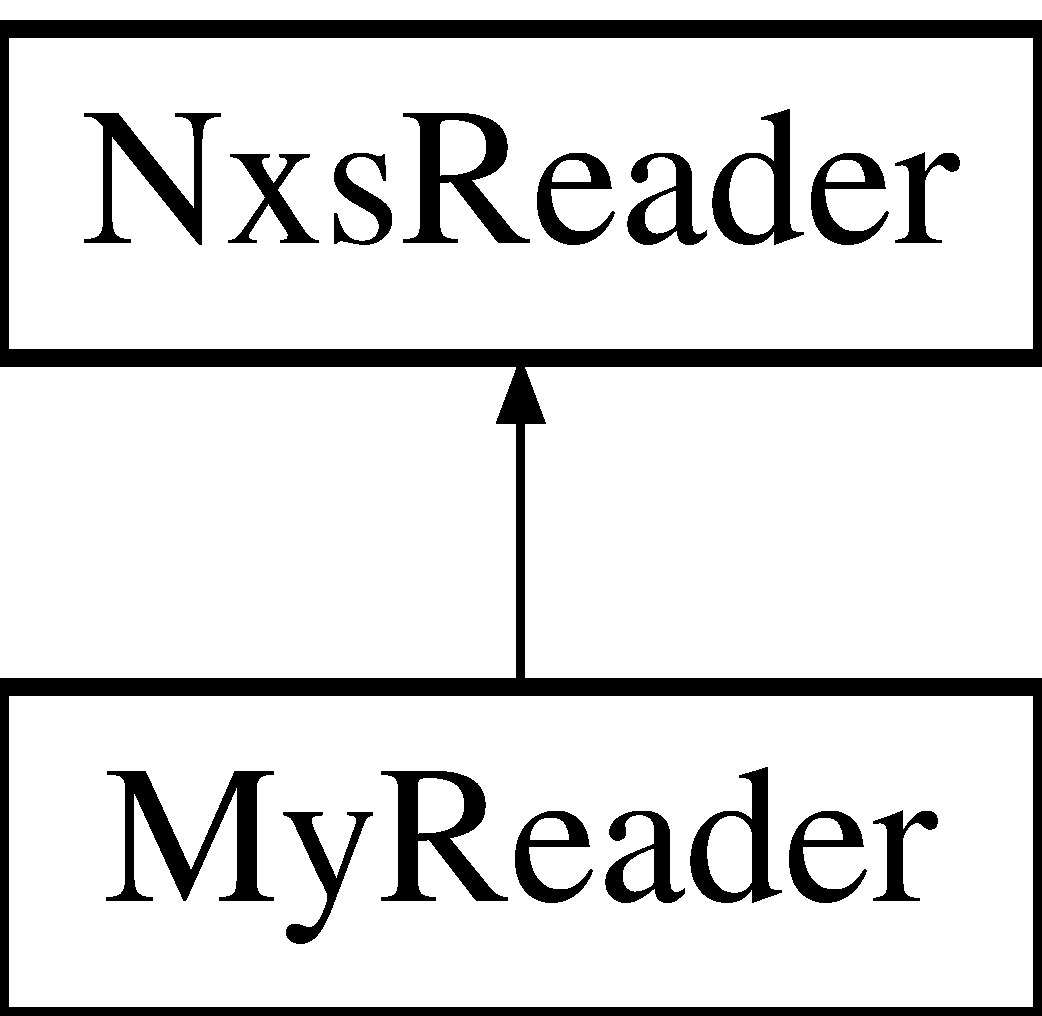
\includegraphics[height=2cm]{classNxsReader}
\end{center}
\end{figure}
\subsection*{Public Types}
\begin{DoxyCompactItemize}
\item 
enum {\bfseries NxsTolerateFlags} \{ {\bfseries allowMissingInEquate} =  0x0001, 
{\bfseries allowPunctuationInNames} =  0x0002
 \}
\end{DoxyCompactItemize}
\subsection*{Public Member Functions}
\begin{DoxyCompactItemize}
\item 
\hypertarget{classNxsReader_a9a3140d103c5aba78f2abb92fe27b73a}{
bool {\bfseries BlockListEmpty} ()}
\label{classNxsReader_a9a3140d103c5aba78f2abb92fe27b73a}

\item 
\hypertarget{classNxsReader_ad8e1a7dcb1c13c88bd1bba769caff29f}{
unsigned {\bfseries PositionInBlockList} (\hyperlink{classNxsBlock}{NxsBlock} $\ast$b)}
\label{classNxsReader_ad8e1a7dcb1c13c88bd1bba769caff29f}

\item 
\hypertarget{classNxsReader_a6d8b9b4cbb59099097a529a4fe6abe39}{
void {\bfseries Add} (\hyperlink{classNxsBlock}{NxsBlock} $\ast$newBlock)}
\label{classNxsReader_a6d8b9b4cbb59099097a529a4fe6abe39}

\item 
\hypertarget{classNxsReader_aa40874a7359e61aef723430c171527e5}{
void {\bfseries Detach} (\hyperlink{classNxsBlock}{NxsBlock} $\ast$newBlock)}
\label{classNxsReader_aa40874a7359e61aef723430c171527e5}

\item 
\hypertarget{classNxsReader_a0a6e516ef15a8c44847a17dc63853fe4}{
void {\bfseries Reassign} (\hyperlink{classNxsBlock}{NxsBlock} $\ast$oldb, \hyperlink{classNxsBlock}{NxsBlock} $\ast$newb)}
\label{classNxsReader_a0a6e516ef15a8c44847a17dc63853fe4}

\item 
\hypertarget{classNxsReader_a57f6e706bac65d43bf5eb2bba3c58a0e}{
void {\bfseries Execute} (\hyperlink{classNxsToken}{NxsToken} \&token, bool notifyStartStop=true)}
\label{classNxsReader_a57f6e706bac65d43bf5eb2bba3c58a0e}

\item 
\hypertarget{classNxsReader_a6be16f40c9f3cbf0028c17dcee96d932}{
virtual void {\bfseries DebugReportBlock} (\hyperlink{classNxsBlock}{NxsBlock} \&nexusBlock)}
\label{classNxsReader_a6be16f40c9f3cbf0028c17dcee96d932}

\item 
\hypertarget{classNxsReader_a22c46391d31a39e4999812698cbcfa30}{
const char $\ast$ {\bfseries NCLNameAndVersion} ()}
\label{classNxsReader_a22c46391d31a39e4999812698cbcfa30}

\item 
\hypertarget{classNxsReader_a1d539ed1e250dcd8a22a7ea3ff9b0cbb}{
const char $\ast$ {\bfseries NCLCopyrightNotice} ()}
\label{classNxsReader_a1d539ed1e250dcd8a22a7ea3ff9b0cbb}

\item 
\hypertarget{classNxsReader_a247cad6e4eeaf06ddeffed70dd6e9b5b}{
const char $\ast$ {\bfseries NCLHomePageURL} ()}
\label{classNxsReader_a247cad6e4eeaf06ddeffed70dd6e9b5b}

\item 
\hypertarget{classNxsReader_ad4468971caafbaa4e17e27ec47174cdd}{
virtual void {\bfseries ExecuteStarting} ()}
\label{classNxsReader_ad4468971caafbaa4e17e27ec47174cdd}

\item 
\hypertarget{classNxsReader_a73220bf4a4db2c3083ba30031972cf02}{
virtual void {\bfseries ExecuteStopping} ()}
\label{classNxsReader_a73220bf4a4db2c3083ba30031972cf02}

\item 
\hypertarget{classNxsReader_a64c3828e9f7ec7061c1a9b7c31b2b783}{
virtual bool {\bfseries EnteringBlock} (\hyperlink{classNxsString}{NxsString} blockName)}
\label{classNxsReader_a64c3828e9f7ec7061c1a9b7c31b2b783}

\item 
\hypertarget{classNxsReader_a6cbf692997601704d4b349108ccaee1a}{
virtual void {\bfseries ExitingBlock} (\hyperlink{classNxsString}{NxsString} blockName)}
\label{classNxsReader_a6cbf692997601704d4b349108ccaee1a}

\item 
\hypertarget{classNxsReader_a86147e9167f9994866f4ba0b34ad0775}{
virtual void {\bfseries OutputComment} (const \hyperlink{classNxsString}{NxsString} \&comment)}
\label{classNxsReader_a86147e9167f9994866f4ba0b34ad0775}

\item 
\hypertarget{classNxsReader_a285ef73c2126ba6ae25d43d95e0ad766}{
virtual void {\bfseries NexusError} (\hyperlink{classNxsString}{NxsString} msg, file\_\-pos pos, long line, long col)}
\label{classNxsReader_a285ef73c2126ba6ae25d43d95e0ad766}

\item 
\hypertarget{classNxsReader_aafc8e7cb840dcc4ded6bcf0a85c4375e}{
virtual void {\bfseries SkippingDisabledBlock} (\hyperlink{classNxsString}{NxsString} blockName)}
\label{classNxsReader_aafc8e7cb840dcc4ded6bcf0a85c4375e}

\item 
\hypertarget{classNxsReader_aa99f543d61a8ed69b1ce4428569ac2a2}{
virtual void {\bfseries SkippingBlock} (\hyperlink{classNxsString}{NxsString} blockName)}
\label{classNxsReader_aa99f543d61a8ed69b1ce4428569ac2a2}

\end{DoxyCompactItemize}
\subsection*{Protected Attributes}
\begin{DoxyCompactItemize}
\item 
\hypertarget{classNxsReader_a655db3db8fbd4ea24a02a9aef3fc872b}{
\hyperlink{classNxsBlock}{NxsBlock} $\ast$ {\bfseries blockList}}
\label{classNxsReader_a655db3db8fbd4ea24a02a9aef3fc872b}

\item 
\hypertarget{classNxsReader_a97928eea97d0cac263162875dedd7afb}{
\hyperlink{classNxsBlock}{NxsBlock} $\ast$ {\bfseries currBlock}}
\label{classNxsReader_a97928eea97d0cac263162875dedd7afb}

\end{DoxyCompactItemize}


The documentation for this class was generated from the following files:\begin{DoxyCompactItemize}
\item 
src/ncl/nxsreader.h\item 
src/ncl/nxsreader.cpp\end{DoxyCompactItemize}

\hypertarget{classNxsSetReader}{
\section{NxsSetReader Class Reference}
\label{classNxsSetReader}\index{NxsSetReader@{NxsSetReader}}
}
\subsection*{Public Types}
\begin{DoxyCompactItemize}
\item 
enum {\bfseries NxsSetReaderEnum} \{ {\bfseries generic} =  1, 
{\bfseries charset}, 
{\bfseries taxset}
 \}
\end{DoxyCompactItemize}
\subsection*{Public Member Functions}
\begin{DoxyCompactItemize}
\item 
\hypertarget{classNxsSetReader_a6db0be01a8a93639a413acd60014200e}{
{\bfseries NxsSetReader} (\hyperlink{classNxsToken}{NxsToken} \&t, unsigned maxValue, NxsUnsignedSet \&iset, \hyperlink{classNxsBlock}{NxsBlock} \&nxsblk, unsigned type)}
\label{classNxsSetReader_a6db0be01a8a93639a413acd60014200e}

\item 
\hypertarget{classNxsSetReader_a28c0f1ed6842b24c5346693d36c0642d}{
bool {\bfseries Run} ()}
\label{classNxsSetReader_a28c0f1ed6842b24c5346693d36c0642d}

\end{DoxyCompactItemize}
\subsection*{Protected Member Functions}
\begin{DoxyCompactItemize}
\item 
\hypertarget{classNxsSetReader_afbb627dcc53f244dbf94539dc49417ea}{
bool {\bfseries AddRange} (unsigned first, unsigned last, unsigned modulus=0)}
\label{classNxsSetReader_afbb627dcc53f244dbf94539dc49417ea}

\end{DoxyCompactItemize}


The documentation for this class was generated from the following files:\begin{DoxyCompactItemize}
\item 
src/ncl/nxssetreader.h\item 
src/ncl/nxssetreader.cpp\end{DoxyCompactItemize}

\hypertarget{classNxsString}{
\section{NxsString Class Reference}
\label{classNxsString}\index{NxsString@{NxsString}}
}
\subsection*{Classes}
\begin{DoxyCompactItemize}
\item 
class \hyperlink{classNxsString_1_1NxsX__NotANumber}{NxsX\_\-NotANumber}
\end{DoxyCompactItemize}
\subsection*{Public Types}
\begin{DoxyCompactItemize}
\item 
enum {\bfseries CmpEnum} \{ {\bfseries respect\_\-case}, 
{\bfseries no\_\-respect\_\-case}, 
{\bfseries abbrev}
 \}
\end{DoxyCompactItemize}
\subsection*{Public Member Functions}
\begin{DoxyCompactItemize}
\item 
\hypertarget{classNxsString_abcd673658cc53d7029dd7196deb65719}{
{\bfseries NxsString} (const char $\ast$s)}
\label{classNxsString_abcd673658cc53d7029dd7196deb65719}

\item 
\hypertarget{classNxsString_a1cea39f14ea5ad1d0a28c6d596003b48}{
{\bfseries NxsString} (const \hyperlink{classNxsString}{NxsString} \&s)}
\label{classNxsString_a1cea39f14ea5ad1d0a28c6d596003b48}

\item 
\hypertarget{classNxsString_af5a5447a725d0772c2a4fb913cc0674c}{
bool {\bfseries Abbreviates} (const \hyperlink{classNxsString}{NxsString} \&s, NxsString::CmpEnum mode=NxsString::no\_\-respect\_\-case) const }
\label{classNxsString_af5a5447a725d0772c2a4fb913cc0674c}

\item 
\hypertarget{classNxsString_af86c992b7d613025ba4ec14bef4e923a}{
unsigned {\bfseries ConvertToUnsigned} () const }
\label{classNxsString_af86c992b7d613025ba4ec14bef4e923a}

\item 
\hypertarget{classNxsString_a195f32f9024ec445e9af4a98d6e1431a}{
int {\bfseries ConvertToInt} () const }
\label{classNxsString_a195f32f9024ec445e9af4a98d6e1431a}

\item 
\hypertarget{classNxsString_a37cb990a4d48d86a2c650cf49f5a7533}{
long {\bfseries ConvertToLong} () const }
\label{classNxsString_a37cb990a4d48d86a2c650cf49f5a7533}

\item 
\hypertarget{classNxsString_ab0ba8827ba9778ace41c65e5c4908471}{
double {\bfseries ConvertToDouble} () const }
\label{classNxsString_ab0ba8827ba9778ace41c65e5c4908471}

\item 
\hypertarget{classNxsString_abd881b99ee0b2a2d9af22ff07fd7a746}{
bool {\bfseries Equals} (const \hyperlink{classNxsString}{NxsString} \&s, NxsString::CmpEnum mode=respect\_\-case) const }
\label{classNxsString_abd881b99ee0b2a2d9af22ff07fd7a746}

\item 
\hypertarget{classNxsString_a1c9d6018f25dd43b0e6795afa25cadd8}{
bool {\bfseries EqualsCaseInsensitive} (const \hyperlink{classNxsString}{NxsString} \&s) const }
\label{classNxsString_a1c9d6018f25dd43b0e6795afa25cadd8}

\item 
\hypertarget{classNxsString_a94c43a042fdd27d06a69beb55abfb09b}{
\hyperlink{classNxsString}{NxsString} {\bfseries GetQuoted} () const }
\label{classNxsString_a94c43a042fdd27d06a69beb55abfb09b}

\item 
\hypertarget{classNxsString_a75e55f7b719838d83e6af1581170dbd9}{
bool {\bfseries IsADouble} () const }
\label{classNxsString_a75e55f7b719838d83e6af1581170dbd9}

\item 
\hypertarget{classNxsString_a71b060209ee38eb8192397ba4459c670}{
bool {\bfseries IsALong} () const }
\label{classNxsString_a71b060209ee38eb8192397ba4459c670}

\item 
\hypertarget{classNxsString_a9b55e9e8030de880de4a9ef2a9c4f3ce}{
bool {\bfseries IsCapAbbreviation} (const \hyperlink{classNxsString}{NxsString} \&s) const }
\label{classNxsString_a9b55e9e8030de880de4a9ef2a9c4f3ce}

\item 
\hypertarget{classNxsString_af4db407b6aad6b6f03fbad6b50f200d2}{
bool {\bfseries IsInVector} (const NxsStringVector \&s, NxsString::CmpEnum mode=respect\_\-case) const }
\label{classNxsString_af4db407b6aad6b6f03fbad6b50f200d2}

\item 
\hypertarget{classNxsString_acaf129f876d1a0471e029e74d79535f8}{
bool {\bfseries IsStdAbbreviation} (const \hyperlink{classNxsString}{NxsString} \&s, bool respectCase) const }
\label{classNxsString_acaf129f876d1a0471e029e74d79535f8}

\item 
\hypertarget{classNxsString_a3c511d513ba1355d94d43b67e263d812}{
bool {\bfseries IsNexusPunctuation} (const char c) const }
\label{classNxsString_a3c511d513ba1355d94d43b67e263d812}

\item 
\hypertarget{classNxsString_ae480dfaa6d3054bc612293cba9821738}{
bool {\bfseries QuotesNeeded} () const }
\label{classNxsString_ae480dfaa6d3054bc612293cba9821738}

\item 
\hypertarget{classNxsString_a32f73ef4a6de84f9f5cf44350bde828d}{
\hyperlink{classNxsString}{NxsString} {\bfseries UpperCasePrefix} () const }
\label{classNxsString_a32f73ef4a6de84f9f5cf44350bde828d}

\item 
\hypertarget{classNxsString_a925aa5c1fd14d364b411e864ab9b2604}{
\hyperlink{classNxsString}{NxsString} \& {\bfseries operator=} (char)}
\label{classNxsString_a925aa5c1fd14d364b411e864ab9b2604}

\item 
\hypertarget{classNxsString_a3636754537192607f211d480f4dfc8cc}{
\hyperlink{classNxsString}{NxsString} \& {\bfseries operator=} (const char $\ast$s)}
\label{classNxsString_a3636754537192607f211d480f4dfc8cc}

\item 
\hypertarget{classNxsString_a4bde9ea22d1e7abed52915e4c6d84b77}{
\hyperlink{classNxsString}{NxsString} \& {\bfseries operator+=} (const char $\ast$s)}
\label{classNxsString_a4bde9ea22d1e7abed52915e4c6d84b77}

\item 
\hypertarget{classNxsString_abf63038f2b7fe55448c0e621295dedf1}{
\hyperlink{classNxsString}{NxsString} \& {\bfseries operator+=} (const \hyperlink{classNxsString}{NxsString} \&s)}
\label{classNxsString_abf63038f2b7fe55448c0e621295dedf1}

\item 
\hypertarget{classNxsString_ad91ba6b582a1b33184d72885363410fe}{
\hyperlink{classNxsString}{NxsString} \& {\bfseries operator+=} (const char c)}
\label{classNxsString_ad91ba6b582a1b33184d72885363410fe}

\item 
\hypertarget{classNxsString_a4bd658ece3ab00a7a1c2789d80f42d3e}{
\hyperlink{classNxsString}{NxsString} \& {\bfseries operator+=} (const int i)}
\label{classNxsString_a4bd658ece3ab00a7a1c2789d80f42d3e}

\item 
\hypertarget{classNxsString_acb657c1ad600c857f42a737bd5f3f58a}{
\hyperlink{classNxsString}{NxsString} \& {\bfseries operator+=} (unsigned i)}
\label{classNxsString_acb657c1ad600c857f42a737bd5f3f58a}

\item 
\hypertarget{classNxsString_a7329e333b6ed7b9caef4102c5bcd5106}{
\hyperlink{classNxsString}{NxsString} \& {\bfseries operator+=} (unsigned long i)}
\label{classNxsString_a7329e333b6ed7b9caef4102c5bcd5106}

\item 
\hypertarget{classNxsString_a2b564181063eb188be85e5c15dc199e7}{
\hyperlink{classNxsString}{NxsString} \& {\bfseries operator+=} (const long l)}
\label{classNxsString_a2b564181063eb188be85e5c15dc199e7}

\item 
\hypertarget{classNxsString_a22901e23a358cdd6f4f7b920cdd5d897}{
\hyperlink{classNxsString}{NxsString} \& {\bfseries operator+=} (const double d)}
\label{classNxsString_a22901e23a358cdd6f4f7b920cdd5d897}

\item 
\hypertarget{classNxsString_af2aacc7c8396f1de338100947fc94ea6}{
\hyperlink{classNxsString}{NxsString} \& {\bfseries operator+=} (const IndexSet \&d)}
\label{classNxsString_af2aacc7c8396f1de338100947fc94ea6}

\item 
\hypertarget{classNxsString_adeb755ab28a88ef19e306cecd9298137}{
\hyperlink{classNxsString}{NxsString} \& {\bfseries operator$<$$<$} (int i)}
\label{classNxsString_adeb755ab28a88ef19e306cecd9298137}

\item 
\hypertarget{classNxsString_a34495041b1536df3ff3d3db73c36e3ab}{
\hyperlink{classNxsString}{NxsString} \& {\bfseries operator$<$$<$} (unsigned i)}
\label{classNxsString_a34495041b1536df3ff3d3db73c36e3ab}

\item 
\hypertarget{classNxsString_a6545e80f1893b1eaa0a4c95f4f898698}{
\hyperlink{classNxsString}{NxsString} \& {\bfseries operator$<$$<$} (long l)}
\label{classNxsString_a6545e80f1893b1eaa0a4c95f4f898698}

\item 
\hypertarget{classNxsString_ae4b766e43d2b2849c3f61de8e33f1d8c}{
\hyperlink{classNxsString}{NxsString} \& {\bfseries operator$<$$<$} (unsigned long l)}
\label{classNxsString_ae4b766e43d2b2849c3f61de8e33f1d8c}

\item 
\hypertarget{classNxsString_a0cacd37439646287ea65199347c37a01}{
\hyperlink{classNxsString}{NxsString} \& {\bfseries operator$<$$<$} (double d)}
\label{classNxsString_a0cacd37439646287ea65199347c37a01}

\item 
\hypertarget{classNxsString_ab50f0327a063eec157fe873d5763f0fb}{
\hyperlink{classNxsString}{NxsString} \& {\bfseries operator$<$$<$} (const char $\ast$c)}
\label{classNxsString_ab50f0327a063eec157fe873d5763f0fb}

\item 
\hypertarget{classNxsString_a5eece8c6a8dacc258afd1da2fdc15606}{
\hyperlink{classNxsString}{NxsString} \& {\bfseries operator$<$$<$} (char c)}
\label{classNxsString_a5eece8c6a8dacc258afd1da2fdc15606}

\item 
\hypertarget{classNxsString_aff7e42d574494ca2982e2c8a3f475890}{
\hyperlink{classNxsString}{NxsString} \& {\bfseries operator$<$$<$} (const \hyperlink{classNxsString}{NxsString} \&s)}
\label{classNxsString_aff7e42d574494ca2982e2c8a3f475890}

\item 
\hypertarget{classNxsString_aa958f87c211324454e01fc4fb3c31432}{
\hyperlink{classNxsString}{NxsString} \& {\bfseries operator$<$$<$} (const IndexSet \&s)}
\label{classNxsString_aa958f87c211324454e01fc4fb3c31432}

\item 
\hypertarget{classNxsString_ae713252b6eb56aab58484a0bb07877a0}{
\hyperlink{classNxsString}{NxsString} \& {\bfseries operator$<$$<$} (\hyperlink{classIndent}{Indent})}
\label{classNxsString_ae713252b6eb56aab58484a0bb07877a0}

\item 
\hypertarget{classNxsString_a7d5287ed3070b7f8fc3fdb8348011ff9}{
\hyperlink{classNxsString}{NxsString} \& {\bfseries operator$<$$<$} (\hyperlink{classNxsString}{NxsString} \&($\ast$funcPtr)(\hyperlink{classNxsString}{NxsString} \&))}
\label{classNxsString_a7d5287ed3070b7f8fc3fdb8348011ff9}

\item 
\hypertarget{classNxsString_abbf904c772d9776139dcae602c9fd06b}{
void {\bfseries clear} ()}
\label{classNxsString_abbf904c772d9776139dcae602c9fd06b}

\item 
\hypertarget{classNxsString_aa306462f5efd5859b5b9e51e3cca4b5f}{
int {\bfseries PrintF} (const char $\ast$formatStr,...)}
\label{classNxsString_aa306462f5efd5859b5b9e51e3cca4b5f}

\item 
\hypertarget{classNxsString_a3e1b16d6ff2fdd61ec12fe93bfb8b777}{
unsigned char $\ast$ {\bfseries p\_\-str} (unsigned char $\ast$) const }
\label{classNxsString_a3e1b16d6ff2fdd61ec12fe93bfb8b777}

\item 
\hypertarget{classNxsString_a8a218e1cef0a63b07699392b5dd057b8}{
\hyperlink{classNxsString}{NxsString} \& {\bfseries AddQuotes} ()}
\label{classNxsString_a8a218e1cef0a63b07699392b5dd057b8}

\item 
\hypertarget{classNxsString_aefdfa11e806b213308bdfe88b6ff9467}{
\hyperlink{classNxsString}{NxsString} \& {\bfseries AddTail} (char c, unsigned n)}
\label{classNxsString_aefdfa11e806b213308bdfe88b6ff9467}

\item 
\hypertarget{classNxsString_a09a3670ce5a889ed02f3cc27afa1fc7d}{
\hyperlink{classNxsString}{NxsString} \& {\bfseries NumberThenWord} (unsigned i, \hyperlink{classNxsString}{NxsString} s)}
\label{classNxsString_a09a3670ce5a889ed02f3cc27afa1fc7d}

\item 
\hypertarget{classNxsString_acd7d1c1d359c1b7ef1e4c8bd8622b802}{
\hyperlink{classNxsString}{NxsString} \& {\bfseries ShortenTo} (unsigned n)}
\label{classNxsString_acd7d1c1d359c1b7ef1e4c8bd8622b802}

\item 
\hypertarget{classNxsString_a7c7a84d57ced24640a02fdbc7be0bbc6}{
\hyperlink{classNxsString}{NxsString} \& {\bfseries AppendDouble} (unsigned minFieldFormat, unsigned precFormat, double x)}
\label{classNxsString_a7c7a84d57ced24640a02fdbc7be0bbc6}

\item 
\hypertarget{classNxsString_a6c8fffe2a4a5f4223671fb5327581e38}{
\hyperlink{classNxsString}{NxsString} \& {\bfseries Capitalize} ()}
\label{classNxsString_a6c8fffe2a4a5f4223671fb5327581e38}

\item 
\hypertarget{classNxsString_a4d0871e7dde794face7cb0f68e8d36ca}{
\hyperlink{classNxsString}{NxsString} \& {\bfseries RightJustifyString} (const \hyperlink{classNxsString}{NxsString} \&s, unsigned w, bool clear\_\-first=false)}
\label{classNxsString_a4d0871e7dde794face7cb0f68e8d36ca}

\item 
\hypertarget{classNxsString_ae7e8aef09b2ec6e928bd881726954bd3}{
\hyperlink{classNxsString}{NxsString} \& {\bfseries RightJustifyLong} (long x, unsigned w, bool clear\_\-first=false)}
\label{classNxsString_ae7e8aef09b2ec6e928bd881726954bd3}

\item 
\hypertarget{classNxsString_a273973a9da80ae8d41d913a2ba9e1def}{
\hyperlink{classNxsString}{NxsString} \& {\bfseries RightJustifyDbl} (double x, unsigned w, unsigned p, bool clear\_\-first=false)}
\label{classNxsString_a273973a9da80ae8d41d913a2ba9e1def}

\item 
\hypertarget{classNxsString_ac32218d5a09d7698a6d1e96a739766e5}{
\hyperlink{classNxsString}{NxsString} \& {\bfseries ToLower} ()}
\label{classNxsString_ac32218d5a09d7698a6d1e96a739766e5}

\item 
\hypertarget{classNxsString_a510af5287bee6eee8227d08715cd0ef4}{
\hyperlink{classNxsString}{NxsString} \& {\bfseries ToUpper} ()}
\label{classNxsString_a510af5287bee6eee8227d08715cd0ef4}

\item 
\hypertarget{classNxsString_a3ff89d00ced11f031db05153b1bbb095}{
\hyperlink{classNxsString}{NxsString} \& {\bfseries BlanksToUnderscores} ()}
\label{classNxsString_a3ff89d00ced11f031db05153b1bbb095}

\item 
\hypertarget{classNxsString_a523fb661c23791d3e0d0d022b62c835c}{
\hyperlink{classNxsString}{NxsString} \& {\bfseries UnderscoresToBlanks} ()}
\label{classNxsString_a523fb661c23791d3e0d0d022b62c835c}

\end{DoxyCompactItemize}
\subsection*{Static Public Member Functions}
\begin{DoxyCompactItemize}
\item 
\hypertarget{classNxsString_ae1ea616b5c58b8efcf4d9310ae557dc4}{
static \hyperlink{classNxsString}{NxsString} {\bfseries ToHex} (long p, unsigned nFours)}
\label{classNxsString_ae1ea616b5c58b8efcf4d9310ae557dc4}

\end{DoxyCompactItemize}
\subsection*{Friends}
\begin{DoxyCompactItemize}
\item 
\hypertarget{classNxsString_a6a6a52802a6cd6fa55b079e03fe65042}{
ostream \& {\bfseries operator$<$$<$} (std::ostream \&out, const \hyperlink{classNxsString}{NxsString} \&s)}
\label{classNxsString_a6a6a52802a6cd6fa55b079e03fe65042}

\end{DoxyCompactItemize}


The documentation for this class was generated from the following files:\begin{DoxyCompactItemize}
\item 
src/ncl/nxsstring.h\item 
src/ncl/nxsstring.cpp\end{DoxyCompactItemize}

\hypertarget{structNxsStringEqual}{
\section{NxsStringEqual Struct Reference}
\label{structNxsStringEqual}\index{NxsStringEqual@{NxsStringEqual}}
}
\subsection*{Public Member Functions}
\begin{DoxyCompactItemize}
\item 
\hypertarget{structNxsStringEqual_aa394cf5616bb90e30a5287eb3422bac0}{
bool {\bfseries operator()} (const \hyperlink{classNxsString}{NxsString} \&x, const \hyperlink{classNxsString}{NxsString} \&y) const }
\label{structNxsStringEqual_aa394cf5616bb90e30a5287eb3422bac0}

\end{DoxyCompactItemize}


The documentation for this struct was generated from the following file:\begin{DoxyCompactItemize}
\item 
src/ncl/nxsstring.h\end{DoxyCompactItemize}

\hypertarget{classNxsTaxaBlock}{
\section{NxsTaxaBlock Class Reference}
\label{classNxsTaxaBlock}\index{NxsTaxaBlock@{NxsTaxaBlock}}
}
Inheritance diagram for NxsTaxaBlock::\begin{figure}[H]
\begin{center}
\leavevmode
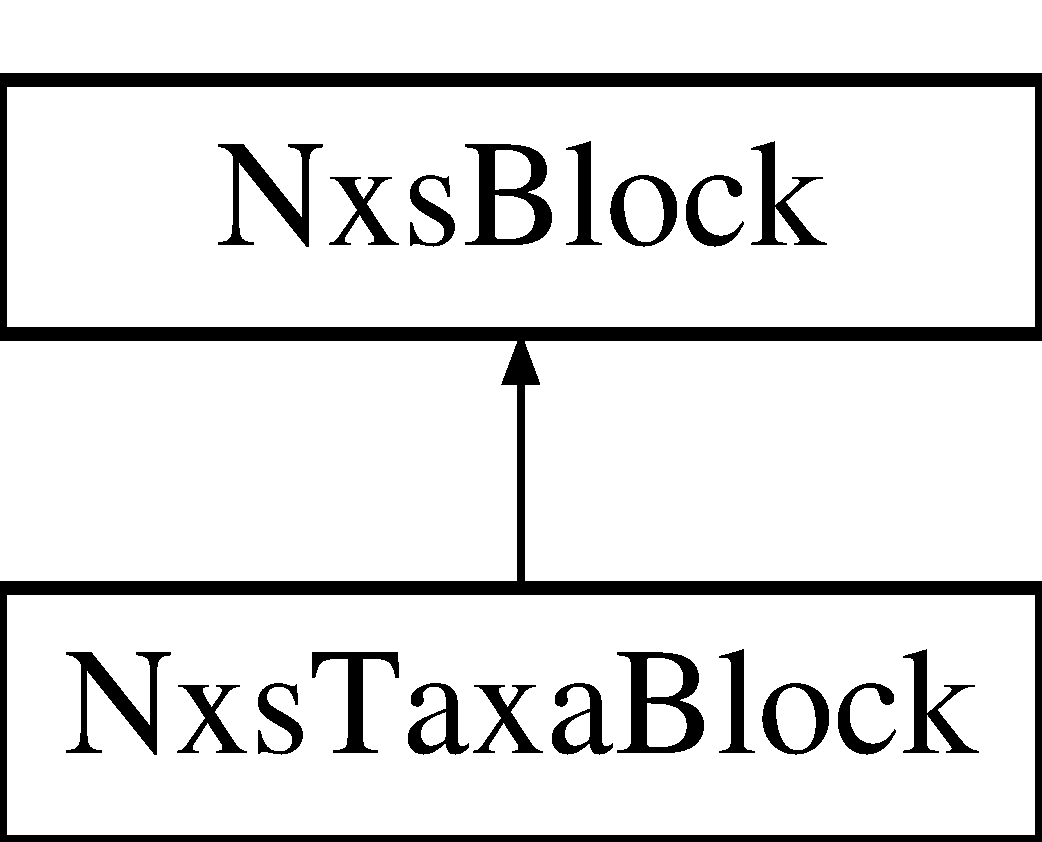
\includegraphics[height=2cm]{classNxsTaxaBlock}
\end{center}
\end{figure}
\subsection*{Classes}
\begin{DoxyCompactItemize}
\item 
class \hyperlink{classNxsTaxaBlock_1_1NxsX__NoSuchTaxon}{NxsX\_\-NoSuchTaxon}
\end{DoxyCompactItemize}
\subsection*{Public Member Functions}
\begin{DoxyCompactItemize}
\item 
\hypertarget{classNxsTaxaBlock_a30181a6a7279c6fcbbaff0bbc0b7b52d}{
virtual unsigned {\bfseries AddTaxonLabel} (\hyperlink{classNxsString}{NxsString} s)}
\label{classNxsTaxaBlock_a30181a6a7279c6fcbbaff0bbc0b7b52d}

\item 
\hypertarget{classNxsTaxaBlock_aebf194e4a18ed394d390bf40c356a809}{
void {\bfseries ChangeTaxonLabel} (unsigned i, \hyperlink{classNxsString}{NxsString} s)}
\label{classNxsTaxaBlock_aebf194e4a18ed394d390bf40c356a809}

\item 
\hypertarget{classNxsTaxaBlock_a1b214b4f3abbd5a0834ae2f4b2dc3e91}{
unsigned {\bfseries FindTaxon} (\hyperlink{classNxsString}{NxsString} label)}
\label{classNxsTaxaBlock_a1b214b4f3abbd5a0834ae2f4b2dc3e91}

\item 
\hypertarget{classNxsTaxaBlock_a0584cfe7dba6c10b8d09292a0cf9cdd2}{
bool {\bfseries IsAlreadyDefined} (\hyperlink{classNxsString}{NxsString} label)}
\label{classNxsTaxaBlock_a0584cfe7dba6c10b8d09292a0cf9cdd2}

\item 
\hypertarget{classNxsTaxaBlock_a81de8995268dbcab73a400762778e743}{
unsigned {\bfseries GetMaxTaxonLabelLength} ()}
\label{classNxsTaxaBlock_a81de8995268dbcab73a400762778e743}

\item 
\hypertarget{classNxsTaxaBlock_aa40174941ba01275db4f9d67fb03dcdf}{
unsigned {\bfseries GetNumTaxonLabels} ()}
\label{classNxsTaxaBlock_aa40174941ba01275db4f9d67fb03dcdf}

\item 
\hypertarget{classNxsTaxaBlock_a52342eda06e07b8eb38f9c5a8bad8cba}{
\hyperlink{classNxsString}{NxsString} {\bfseries GetTaxonLabel} (unsigned i)}
\label{classNxsTaxaBlock_a52342eda06e07b8eb38f9c5a8bad8cba}

\item 
\hypertarget{classNxsTaxaBlock_a8dd12e868709d36640456c5b59983f8a}{
bool {\bfseries NeedsQuotes} (unsigned i)}
\label{classNxsTaxaBlock_a8dd12e868709d36640456c5b59983f8a}

\item 
\hypertarget{classNxsTaxaBlock_a0b0fd6be375b3bc6f14603da640c7659}{
virtual void {\bfseries Report} (ostream \&out)}
\label{classNxsTaxaBlock_a0b0fd6be375b3bc6f14603da640c7659}

\item 
\hypertarget{classNxsTaxaBlock_a9787a850ce00e40428696b93b1669020}{
virtual void {\bfseries Reset} ()}
\label{classNxsTaxaBlock_a9787a850ce00e40428696b93b1669020}

\end{DoxyCompactItemize}
\subsection*{Protected Member Functions}
\begin{DoxyCompactItemize}
\item 
\hypertarget{classNxsTaxaBlock_ad2f6ed5bca65a4f13297b96f5ce2c103}{
virtual void {\bfseries Read} (\hyperlink{classNxsToken}{NxsToken} \&token)}
\label{classNxsTaxaBlock_ad2f6ed5bca65a4f13297b96f5ce2c103}

\end{DoxyCompactItemize}
\subsection*{Protected Attributes}
\begin{DoxyCompactItemize}
\item 
\hypertarget{classNxsTaxaBlock_abd5df0c58e31ddfa79d1590684708323}{
unsigned {\bfseries ntax}}
\label{classNxsTaxaBlock_abd5df0c58e31ddfa79d1590684708323}

\item 
\hypertarget{classNxsTaxaBlock_ad60b4588aa924cf2a99b4101d0477adc}{
NxsStringVector {\bfseries taxonLabels}}
\label{classNxsTaxaBlock_ad60b4588aa924cf2a99b4101d0477adc}

\item 
\hypertarget{classNxsTaxaBlock_ae69aaf354301e536f5b9524dc5e3f3de}{
NxsBoolVector {\bfseries needsQuotes}}
\label{classNxsTaxaBlock_ae69aaf354301e536f5b9524dc5e3f3de}

\end{DoxyCompactItemize}
\subsection*{Friends}
\begin{DoxyCompactItemize}
\item 
\hypertarget{classNxsTaxaBlock_a69ad16654c829e898a92c569c7fa8b8d}{
class \hyperlink{classNxsTaxaBlock_a69ad16654c829e898a92c569c7fa8b8d}{NxsDataBlock}}
\label{classNxsTaxaBlock_a69ad16654c829e898a92c569c7fa8b8d}

\item 
\hypertarget{classNxsTaxaBlock_ad9ba2bb6bba16b181df5d60f0c244681}{
class {\bfseries NxsAllelesBlock}}
\label{classNxsTaxaBlock_ad9ba2bb6bba16b181df5d60f0c244681}

\item 
\hypertarget{classNxsTaxaBlock_ab9466d1b21f90b6fd961284f19c6e9d4}{
class \hyperlink{classNxsTaxaBlock_ab9466d1b21f90b6fd961284f19c6e9d4}{NxsCharactersBlock}}
\label{classNxsTaxaBlock_ab9466d1b21f90b6fd961284f19c6e9d4}

\item 
\hypertarget{classNxsTaxaBlock_aa46e2fbd4a6264cf2f0f91035cdf6188}{
class \hyperlink{classNxsTaxaBlock_aa46e2fbd4a6264cf2f0f91035cdf6188}{NxsDistancesBlock}}
\label{classNxsTaxaBlock_aa46e2fbd4a6264cf2f0f91035cdf6188}

\end{DoxyCompactItemize}


The documentation for this class was generated from the following files:\begin{DoxyCompactItemize}
\item 
src/ncl/nxstaxablock.h\item 
src/ncl/nxstaxablock.cpp\end{DoxyCompactItemize}

\hypertarget{classNxsToken}{
\section{NxsToken Class Reference}
\label{classNxsToken}\index{NxsToken@{NxsToken}}
}
Inheritance diagram for NxsToken::\begin{figure}[H]
\begin{center}
\leavevmode
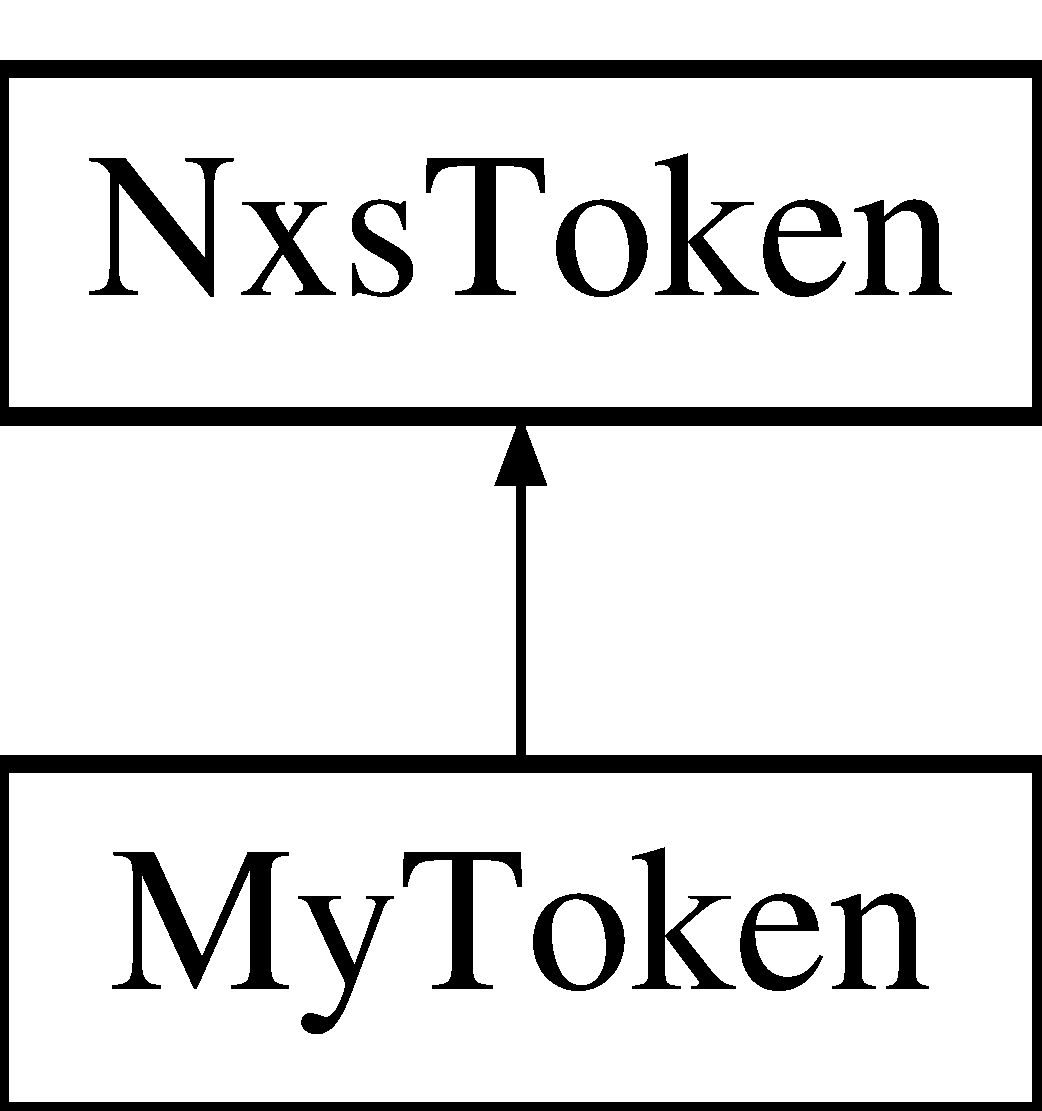
\includegraphics[height=2cm]{classNxsToken}
\end{center}
\end{figure}
\subsection*{Public Types}
\begin{DoxyCompactItemize}
\item 
enum {\bfseries NxsTokenFlags} \{ \par
{\bfseries saveCommandComments} =  0x0001, 
{\bfseries parentheticalToken} =  0x0002, 
{\bfseries curlyBracketedToken} =  0x0004, 
{\bfseries doubleQuotedToken} =  0x0008, 
\par
{\bfseries singleCharacterToken} =  0x0010, 
{\bfseries newlineIsToken} =  0x0020, 
{\bfseries tildeIsPunctuation} =  0x0040, 
{\bfseries useSpecialPunctuation} =  0x0080, 
\par
{\bfseries hyphenNotPunctuation} =  0x0100, 
{\bfseries preserveUnderscores} =  0x0200, 
{\bfseries ignorePunctuation} =  0x0400
 \}
\end{DoxyCompactItemize}
\subsection*{Public Member Functions}
\begin{DoxyCompactItemize}
\item 
\hypertarget{classNxsToken_aa7932e5bf17ccae942e64d9cb1f6ae4c}{
{\bfseries NxsToken} (istream \&i)}
\label{classNxsToken_aa7932e5bf17ccae942e64d9cb1f6ae4c}

\item 
\hypertarget{classNxsToken_a54326092fbb2974720ddbc2ea176bb65}{
bool {\bfseries AtEOF} ()}
\label{classNxsToken_a54326092fbb2974720ddbc2ea176bb65}

\item 
\hypertarget{classNxsToken_ad2671eb776f8f76ac946fd5b76e93c0a}{
bool {\bfseries AtEOL} ()}
\label{classNxsToken_ad2671eb776f8f76ac946fd5b76e93c0a}

\item 
\hypertarget{classNxsToken_a27b278f4a91b233ec6412d1359ed4e04}{
bool {\bfseries Abbreviation} (\hyperlink{classNxsString}{NxsString} s)}
\label{classNxsToken_a27b278f4a91b233ec6412d1359ed4e04}

\item 
\hypertarget{classNxsToken_a8982d8c087b1c10ffd794c1689e0acea}{
bool {\bfseries Begins} (\hyperlink{classNxsString}{NxsString} s, bool respect\_\-case=false)}
\label{classNxsToken_a8982d8c087b1c10ffd794c1689e0acea}

\item 
\hypertarget{classNxsToken_adaffa5866ddf0a39a26a5e436183b9c5}{
void {\bfseries BlanksToUnderscores} ()}
\label{classNxsToken_adaffa5866ddf0a39a26a5e436183b9c5}

\item 
\hypertarget{classNxsToken_a339c42adadfab9d221581d6d64208b80}{
bool {\bfseries Equals} (\hyperlink{classNxsString}{NxsString} s, bool respect\_\-case=false)}
\label{classNxsToken_a339c42adadfab9d221581d6d64208b80}

\item 
\hypertarget{classNxsToken_a7272fd1469fa6424086a95ec4f92eab0}{
long {\bfseries GetFileColumn} () const }
\label{classNxsToken_a7272fd1469fa6424086a95ec4f92eab0}

\item 
\hypertarget{classNxsToken_a17e5caf91acc756c23159f76f8b2d0fd}{
file\_\-pos {\bfseries GetFilePosition} () const }
\label{classNxsToken_a17e5caf91acc756c23159f76f8b2d0fd}

\item 
\hypertarget{classNxsToken_ae0fb11bf350d907295447864afa714ec}{
long {\bfseries GetFileLine} () const }
\label{classNxsToken_ae0fb11bf350d907295447864afa714ec}

\item 
\hypertarget{classNxsToken_a3346e398b3f6b5e8c7c3cebc49ae1c4b}{
void {\bfseries GetNextToken} ()}
\label{classNxsToken_a3346e398b3f6b5e8c7c3cebc49ae1c4b}

\item 
\hypertarget{classNxsToken_a83d7b2a9a2307a0aee8476b904c8145f}{
\hyperlink{classNxsString}{NxsString} {\bfseries GetToken} (bool respect\_\-case=true)}
\label{classNxsToken_a83d7b2a9a2307a0aee8476b904c8145f}

\item 
\hypertarget{classNxsToken_abb9c1599e43267a342fb72be7b878541}{
const char $\ast$ {\bfseries GetTokenAsCStr} (bool respect\_\-case=true)}
\label{classNxsToken_abb9c1599e43267a342fb72be7b878541}

\item 
\hypertarget{classNxsToken_aba7767f4b14936fa7061b77cf2f9e543}{
const \hyperlink{classNxsString}{NxsString} \& {\bfseries GetTokenReference} ()}
\label{classNxsToken_aba7767f4b14936fa7061b77cf2f9e543}

\item 
\hypertarget{classNxsToken_a8231aba780039e4ef1fe2fbf24e21dba}{
int {\bfseries GetTokenLength} () const }
\label{classNxsToken_a8231aba780039e4ef1fe2fbf24e21dba}

\item 
\hypertarget{classNxsToken_af75d27ce09e09c66c838ad61e13839f7}{
bool {\bfseries IsPlusMinusToken} ()}
\label{classNxsToken_af75d27ce09e09c66c838ad61e13839f7}

\item 
\hypertarget{classNxsToken_a0e5bcf6a302bf475420b28036a218b51}{
bool {\bfseries IsPunctuationToken} ()}
\label{classNxsToken_a0e5bcf6a302bf475420b28036a218b51}

\item 
\hypertarget{classNxsToken_ada43d5e71e16665d7f20874bd6fb6641}{
bool {\bfseries IsWhitespaceToken} ()}
\label{classNxsToken_ada43d5e71e16665d7f20874bd6fb6641}

\item 
\hypertarget{classNxsToken_ac77db1862982198172efd9bc908d8e38}{
void {\bfseries ReplaceToken} (const \hyperlink{classNxsString}{NxsString} s)}
\label{classNxsToken_ac77db1862982198172efd9bc908d8e38}

\item 
\hypertarget{classNxsToken_afd330ed87b253864f10dd8c4282d824d}{
void {\bfseries ResetToken} ()}
\label{classNxsToken_afd330ed87b253864f10dd8c4282d824d}

\item 
\hypertarget{classNxsToken_ad6e4423d22411f5779f2043f22008256}{
void {\bfseries SetSpecialPunctuationCharacter} (char c)}
\label{classNxsToken_ad6e4423d22411f5779f2043f22008256}

\item 
\hypertarget{classNxsToken_afa5232738ca19e069173e8befe75e730}{
void {\bfseries SetLabileFlagBit} (int bit)}
\label{classNxsToken_afa5232738ca19e069173e8befe75e730}

\item 
\hypertarget{classNxsToken_a866fd0156710932ff8cc9aeeccde3fa6}{
bool {\bfseries StoppedOn} (char ch)}
\label{classNxsToken_a866fd0156710932ff8cc9aeeccde3fa6}

\item 
\hypertarget{classNxsToken_a1c6fa60bd11ed8df496ea30083005532}{
void {\bfseries StripWhitespace} ()}
\label{classNxsToken_a1c6fa60bd11ed8df496ea30083005532}

\item 
\hypertarget{classNxsToken_a19a122c7b27d6cda65034acee1d61d01}{
void {\bfseries ToUpper} ()}
\label{classNxsToken_a19a122c7b27d6cda65034acee1d61d01}

\item 
\hypertarget{classNxsToken_a0ae503db53d3e2ec1e194505575e9721}{
void {\bfseries Write} (ostream \&out)}
\label{classNxsToken_a0ae503db53d3e2ec1e194505575e9721}

\item 
\hypertarget{classNxsToken_afb060151230ba6d764dd894f5e50b075}{
void {\bfseries Writeln} (ostream \&out)}
\label{classNxsToken_afb060151230ba6d764dd894f5e50b075}

\item 
\hypertarget{classNxsToken_a8bcc10cb8b852257dc0449491e74cbff}{
virtual void {\bfseries OutputComment} (const \hyperlink{classNxsString}{NxsString} \&msg)}
\label{classNxsToken_a8bcc10cb8b852257dc0449491e74cbff}

\end{DoxyCompactItemize}
\subsection*{Public Attributes}
\begin{DoxyCompactItemize}
\item 
\hypertarget{classNxsToken_a30b21153e170902dbfd8554a10c982ea}{
\hyperlink{classNxsString}{NxsString} {\bfseries errormsg}}
\label{classNxsToken_a30b21153e170902dbfd8554a10c982ea}

\end{DoxyCompactItemize}
\subsection*{Protected Member Functions}
\begin{DoxyCompactItemize}
\item 
\hypertarget{classNxsToken_aa142a5a69e1c72baf998e368f727ffee}{
void {\bfseries AppendToComment} (char ch)}
\label{classNxsToken_aa142a5a69e1c72baf998e368f727ffee}

\item 
\hypertarget{classNxsToken_afb74dbfb0fa6a930fd33ef59e235f710}{
void {\bfseries AppendToToken} (char ch)}
\label{classNxsToken_afb74dbfb0fa6a930fd33ef59e235f710}

\item 
\hypertarget{classNxsToken_a4f192c1a77663b4de509e0838929d312}{
char {\bfseries GetNextChar} ()}
\label{classNxsToken_a4f192c1a77663b4de509e0838929d312}

\item 
\hypertarget{classNxsToken_aad4d827a0814f56659327415508c9d79}{
void {\bfseries GetComment} ()}
\label{classNxsToken_aad4d827a0814f56659327415508c9d79}

\item 
\hypertarget{classNxsToken_a795e4e69cf60a1d2d61db352f79aedd2}{
void {\bfseries GetCurlyBracketedToken} ()}
\label{classNxsToken_a795e4e69cf60a1d2d61db352f79aedd2}

\item 
\hypertarget{classNxsToken_a574341a2ecd844630d340a28e64ff413}{
void {\bfseries GetDoubleQuotedToken} ()}
\label{classNxsToken_a574341a2ecd844630d340a28e64ff413}

\item 
\hypertarget{classNxsToken_a76bc1b62bee1e6de6a9ab2e01d720517}{
void {\bfseries GetQuoted} ()}
\label{classNxsToken_a76bc1b62bee1e6de6a9ab2e01d720517}

\item 
\hypertarget{classNxsToken_ad73bcb3d0feecbbf86d2b3b017667047}{
void {\bfseries GetParentheticalToken} ()}
\label{classNxsToken_ad73bcb3d0feecbbf86d2b3b017667047}

\item 
\hypertarget{classNxsToken_ace5934a87892ba50ebea2c1b93866dc3}{
bool {\bfseries IsPunctuation} (char ch)}
\label{classNxsToken_ace5934a87892ba50ebea2c1b93866dc3}

\item 
\hypertarget{classNxsToken_a4362f9387840f57ebde0f7aa5bf6d4c8}{
bool {\bfseries IsWhitespace} (char ch)}
\label{classNxsToken_a4362f9387840f57ebde0f7aa5bf6d4c8}

\end{DoxyCompactItemize}


The documentation for this class was generated from the following files:\begin{DoxyCompactItemize}
\item 
src/ncl/nxstoken.h\item 
src/ncl/nxstoken.cpp\end{DoxyCompactItemize}

\hypertarget{classNxsTreesBlock}{
\section{NxsTreesBlock Class Reference}
\label{classNxsTreesBlock}\index{NxsTreesBlock@{NxsTreesBlock}}
}
Inheritance diagram for NxsTreesBlock::\begin{figure}[H]
\begin{center}
\leavevmode
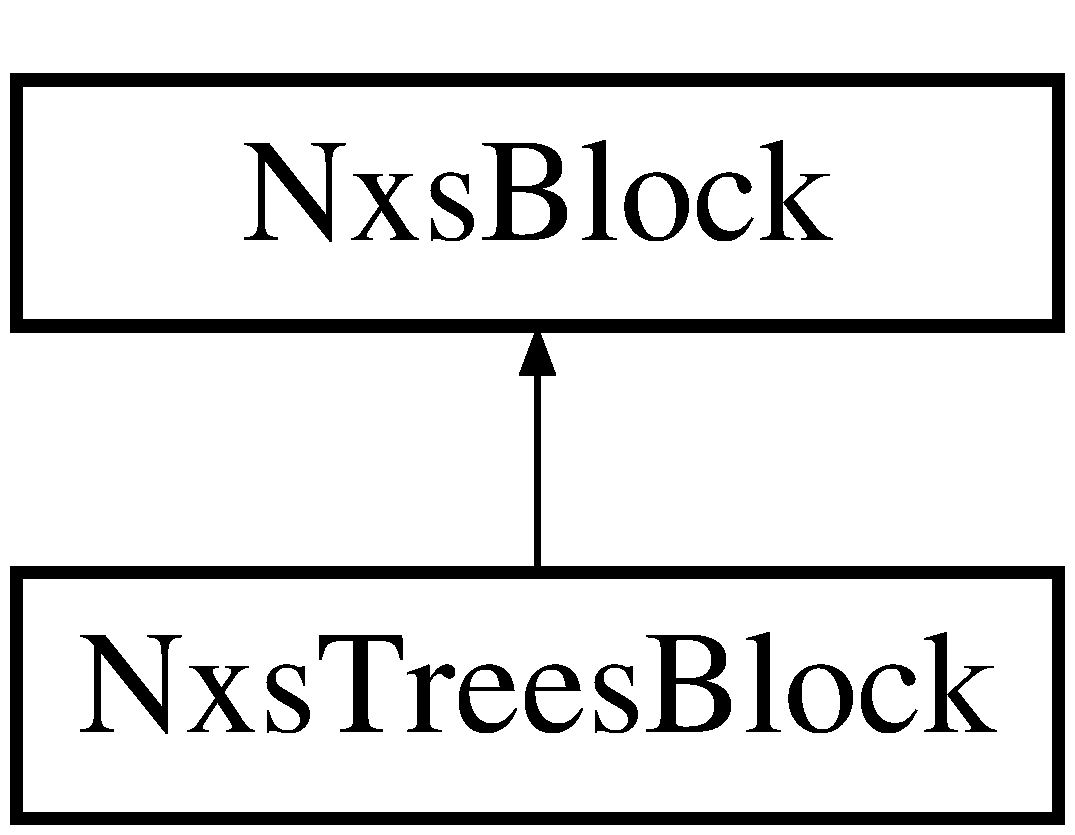
\includegraphics[height=2cm]{classNxsTreesBlock}
\end{center}
\end{figure}
\subsection*{Public Member Functions}
\begin{DoxyCompactItemize}
\item 
\hypertarget{classNxsTreesBlock_a704547f062feafaf84297830b402e8eb}{
{\bfseries NxsTreesBlock} (\hyperlink{classNxsTaxaBlock}{NxsTaxaBlock} $\ast$tb)}
\label{classNxsTreesBlock_a704547f062feafaf84297830b402e8eb}

\item 
\hypertarget{classNxsTreesBlock_ad28d89fdc04168557dcfeaf287311340}{
void {\bfseries ReplaceTaxaBlockPtr} (\hyperlink{classNxsTaxaBlock}{NxsTaxaBlock} $\ast$tb)}
\label{classNxsTreesBlock_ad28d89fdc04168557dcfeaf287311340}

\item 
\hypertarget{classNxsTreesBlock_ac0b38cb4008db1b378aa4dd0d2860bd3}{
unsigned {\bfseries GetNumDefaultTree} ()}
\label{classNxsTreesBlock_ac0b38cb4008db1b378aa4dd0d2860bd3}

\item 
\hypertarget{classNxsTreesBlock_ab8482cf659047135f64473ae241eae70}{
unsigned {\bfseries GetNumTrees} ()}
\label{classNxsTreesBlock_ab8482cf659047135f64473ae241eae70}

\item 
\hypertarget{classNxsTreesBlock_a6498e89a41074ff0f3f330b89c6abb06}{
\hyperlink{classNxsString}{NxsString} {\bfseries GetTreeName} (unsigned i)}
\label{classNxsTreesBlock_a6498e89a41074ff0f3f330b89c6abb06}

\item 
\hypertarget{classNxsTreesBlock_aa00e91e2ff1a4482d6c162ccc3486eef}{
\hyperlink{classNxsString}{NxsString} {\bfseries GetTreeDescription} (unsigned i)}
\label{classNxsTreesBlock_aa00e91e2ff1a4482d6c162ccc3486eef}

\item 
\hypertarget{classNxsTreesBlock_aad4276c6d0813bfafb138f55a6f42ad5}{
\hyperlink{classNxsString}{NxsString} {\bfseries GetTranslatedTreeDescription} (unsigned i)}
\label{classNxsTreesBlock_aad4276c6d0813bfafb138f55a6f42ad5}

\item 
\hypertarget{classNxsTreesBlock_a497c23c2acca696f9248ab88bf2db946}{
bool {\bfseries IsDefaultTree} (unsigned i)}
\label{classNxsTreesBlock_a497c23c2acca696f9248ab88bf2db946}

\item 
\hypertarget{classNxsTreesBlock_aee81a3a2830bd695566e3b0d1b5d079f}{
bool {\bfseries IsRootedTree} (unsigned i)}
\label{classNxsTreesBlock_aee81a3a2830bd695566e3b0d1b5d079f}

\item 
\hypertarget{classNxsTreesBlock_a0303349f1351d4a00f20be5130783fa9}{
virtual void {\bfseries Report} (std::ostream \&out)}
\label{classNxsTreesBlock_a0303349f1351d4a00f20be5130783fa9}

\item 
\hypertarget{classNxsTreesBlock_ab6f6fde301d28f9082acca328b1cddcc}{
virtual void {\bfseries BriefReport} (\hyperlink{classNxsString}{NxsString} \&s)}
\label{classNxsTreesBlock_ab6f6fde301d28f9082acca328b1cddcc}

\item 
\hypertarget{classNxsTreesBlock_aebea09e1b7b01331ee2f89beee2ece46}{
virtual void {\bfseries Reset} ()}
\label{classNxsTreesBlock_aebea09e1b7b01331ee2f89beee2ece46}

\end{DoxyCompactItemize}
\subsection*{Protected Member Functions}
\begin{DoxyCompactItemize}
\item 
\hypertarget{classNxsTreesBlock_a60a667c2b280c08ddd2608e0b2aff9d3}{
virtual void {\bfseries Read} (\hyperlink{classNxsToken}{NxsToken} \&token)}
\label{classNxsTreesBlock_a60a667c2b280c08ddd2608e0b2aff9d3}

\item 
\hypertarget{classNxsTreesBlock_ad54cdad1ec707602b1468af2962f5b15}{
void {\bfseries HandleTreeDescription} (\hyperlink{classNxsToken}{NxsToken} \&token, bool utree)}
\label{classNxsTreesBlock_ad54cdad1ec707602b1468af2962f5b15}

\end{DoxyCompactItemize}
\subsection*{Protected Attributes}
\begin{DoxyCompactItemize}
\item 
\hypertarget{classNxsTreesBlock_a9b98704435d1d19b44e0413bc683501a}{
NxsStringMap {\bfseries translateList}}
\label{classNxsTreesBlock_a9b98704435d1d19b44e0413bc683501a}

\item 
\hypertarget{classNxsTreesBlock_a783481691f6eb6f76ededc08ef54b88e}{
NxsStringVector {\bfseries treeName}}
\label{classNxsTreesBlock_a783481691f6eb6f76ededc08ef54b88e}

\item 
\hypertarget{classNxsTreesBlock_add8b39382c1adbb4d2be37ddce1d983b}{
NxsStringVector {\bfseries treeDescription}}
\label{classNxsTreesBlock_add8b39382c1adbb4d2be37ddce1d983b}

\item 
\hypertarget{classNxsTreesBlock_a96b97e6ca078dd1405a3bf0a20e3de1f}{
NxsBoolVector {\bfseries rooted}}
\label{classNxsTreesBlock_a96b97e6ca078dd1405a3bf0a20e3de1f}

\item 
\hypertarget{classNxsTreesBlock_aa0e5a09dd29bbcdd4b18b0870e01b2d8}{
\hyperlink{classNxsTaxaBlock}{NxsTaxaBlock} $\ast$ {\bfseries taxa}}
\label{classNxsTreesBlock_aa0e5a09dd29bbcdd4b18b0870e01b2d8}

\item 
\hypertarget{classNxsTreesBlock_a8c3a9f04200ab3d2ed4072cbd636b9c8}{
unsigned {\bfseries ntrees}}
\label{classNxsTreesBlock_a8c3a9f04200ab3d2ed4072cbd636b9c8}

\item 
\hypertarget{classNxsTreesBlock_aeb1d8248a0840568c429776bc0246821}{
unsigned {\bfseries defaultTree}}
\label{classNxsTreesBlock_aeb1d8248a0840568c429776bc0246821}

\end{DoxyCompactItemize}


The documentation for this class was generated from the following files:\begin{DoxyCompactItemize}
\item 
src/ncl/nxstreesblock.h\item 
src/ncl/nxstreesblock.cpp\end{DoxyCompactItemize}

\hypertarget{classNxsTaxaBlock_1_1NxsX__NoSuchTaxon}{
\section{NxsTaxaBlock::NxsX\_\-NoSuchTaxon Class Reference}
\label{classNxsTaxaBlock_1_1NxsX__NoSuchTaxon}\index{NxsTaxaBlock::NxsX\_\-NoSuchTaxon@{NxsTaxaBlock::NxsX\_\-NoSuchTaxon}}
}


The documentation for this class was generated from the following file:\begin{DoxyCompactItemize}
\item 
src/ncl/nxstaxablock.h\end{DoxyCompactItemize}

\hypertarget{classNxsString_1_1NxsX__NotANumber}{
\section{NxsString::NxsX\_\-NotANumber Class Reference}
\label{classNxsString_1_1NxsX__NotANumber}\index{NxsString::NxsX\_\-NotANumber@{NxsString::NxsX\_\-NotANumber}}
}


The documentation for this class was generated from the following file:\begin{DoxyCompactItemize}
\item 
src/ncl/nxsstring.h\end{DoxyCompactItemize}

\hypertarget{classOptimization}{
\section{Optimization Class Reference}
\label{classOptimization}\index{Optimization@{Optimization}}
}


{\ttfamily \#include $<$optimization.h$>$}Inheritance diagram for Optimization::\begin{figure}[H]
\begin{center}
\leavevmode
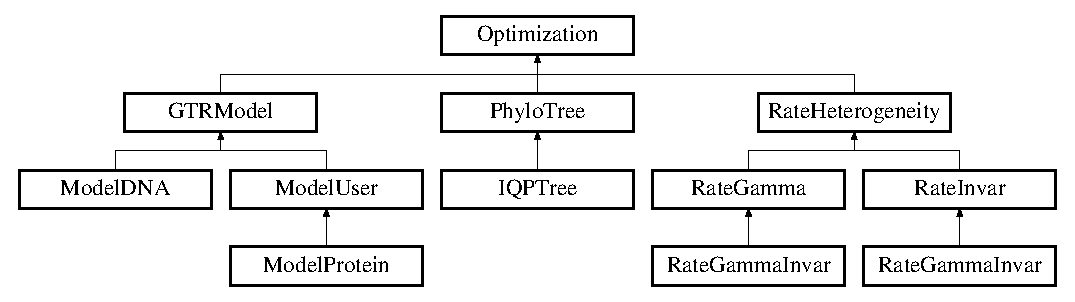
\includegraphics[height=3.6129cm]{classOptimization}
\end{center}
\end{figure}
\subsection*{Public Member Functions}
\begin{DoxyCompactItemize}
\item 
virtual double \hyperlink{classOptimization_ad7ca7b884076f8c76312d516e23c6609}{computeFunction} (double value)
\item 
double \hyperlink{classOptimization_a59ccdfae81744716ce48226da029d470}{minimizeOneDimen} (double xmin, double xguess, double xmax, double tolerance, double $\ast$fx, double $\ast$ferror)
\item 
virtual double \hyperlink{classOptimization_a18bedacde6fd259ff5923c9e936464bd}{computeFuncDerv} (double value, double \&df, double \&ddf)
\item 
double \hyperlink{classOptimization_a32d3810b12230f4201e03ea25f0320ec}{minimizeNewton} (double xmin, double xguess, double xmax, double tolerance, double \&f)
\item 
virtual int \hyperlink{classOptimization_a6d04cefb0969f3cac9b607aa1412eb57}{getNDim} ()
\item 
virtual double \hyperlink{classOptimization_a7fe7c6178977ef7840ff65d216bf590e}{targetFunk} (double x\mbox{[}$\,$\mbox{]})
\item 
virtual double \hyperlink{classOptimization_a804d1f309afd4285d62bc48b6c00338a}{derivativeFunk} (double x\mbox{[}$\,$\mbox{]}, double dfx\mbox{[}$\,$\mbox{]})
\item 
virtual bool \hyperlink{classOptimization_aa80661f2519aa3a9f1521309e854acfc}{checkRange} (double x\mbox{[}$\,$\mbox{]})
\item 
double \hyperlink{classOptimization_a2e263d2334c328f6a0a8429bc901a42b}{minimizeMultiDimen} (double guess\mbox{[}$\,$\mbox{]}, int ndim, double lower\mbox{[}$\,$\mbox{]}, double upper\mbox{[}$\,$\mbox{]}, bool bound\_\-check\mbox{[}$\,$\mbox{]}, double gtol)
\end{DoxyCompactItemize}


\subsection{Detailed Description}
\hyperlink{classOptimization}{Optimization} class, implement some methods like Brent, Newton-\/Raphson (for 1 variable function), BFGS (for multi-\/dimensional function)

\begin{DoxyAuthor}{Author}
BUI Quang Minh, Steffen Klaere, Arndt von Haeseler $<$\href{mailto:minh.bui@univie.ac.at}{\tt minh.bui@univie.ac.at}$>$ 
\end{DoxyAuthor}


\subsection{Member Function Documentation}
\hypertarget{classOptimization_aa80661f2519aa3a9f1521309e854acfc}{
\index{Optimization@{Optimization}!checkRange@{checkRange}}
\index{checkRange@{checkRange}!Optimization@{Optimization}}
\subsubsection[{checkRange}]{\setlength{\rightskip}{0pt plus 5cm}virtual bool Optimization::checkRange (double {\em x}\mbox{[}$\,$\mbox{]})\hspace{0.3cm}{\ttfamily  \mbox{[}inline, virtual\mbox{]}}}}
\label{classOptimization_aa80661f2519aa3a9f1521309e854acfc}
check of range of parameters \hypertarget{classOptimization_a18bedacde6fd259ff5923c9e936464bd}{
\index{Optimization@{Optimization}!computeFuncDerv@{computeFuncDerv}}
\index{computeFuncDerv@{computeFuncDerv}!Optimization@{Optimization}}
\subsubsection[{computeFuncDerv}]{\setlength{\rightskip}{0pt plus 5cm}virtual double Optimization::computeFuncDerv (double {\em value}, \/  double \& {\em df}, \/  double \& {\em ddf})\hspace{0.3cm}{\ttfamily  \mbox{[}inline, virtual\mbox{]}}}}
\label{classOptimization_a18bedacde6fd259ff5923c9e936464bd}
This function calculate f(value), first derivative f'(value) and 2nd derivative f''(value). used by Newton raphson method to minimize the function. Please always override this function to adapt to likelihood or parsimony score. The default is for function f(x) = x$^\wedge$2. 
\begin{DoxyParams}{Parameters}
\item[{\em value}]x-\/value of the function \item[{\em df}](OUT) first derivative \item[{\em ddf}](OUT) second derivative \end{DoxyParams}
\begin{DoxyReturn}{Returns}
f(value) of function f you want to minimize 
\end{DoxyReturn}


Reimplemented in \hyperlink{classPhyloTree_a9ae5f61aa0d22976b2d2e8f3ed15f44f}{PhyloTree}.\hypertarget{classOptimization_ad7ca7b884076f8c76312d516e23c6609}{
\index{Optimization@{Optimization}!computeFunction@{computeFunction}}
\index{computeFunction@{computeFunction}!Optimization@{Optimization}}
\subsubsection[{computeFunction}]{\setlength{\rightskip}{0pt plus 5cm}virtual double Optimization::computeFunction (double {\em value})\hspace{0.3cm}{\ttfamily  \mbox{[}inline, virtual\mbox{]}}}}
\label{classOptimization_ad7ca7b884076f8c76312d516e23c6609}
This function calculate f(value) of the f() function, used by other general optimization method to minimize it. Please always override this function to adapt to likelihood or parsimony score. The default is for function f(x)=x. 
\begin{DoxyParams}{Parameters}
\item[{\em value}]x-\/value of the function \end{DoxyParams}
\begin{DoxyReturn}{Returns}
f(value) of function f you want to minimize 
\end{DoxyReturn}


Reimplemented in \hyperlink{classPhyloTree_a34c7bdc00d48d66e1a8ebfee9af1f100}{PhyloTree}, \hyperlink{classRateGamma_a24e01b7ec0d9170ceebcf03b603b2bbb}{RateGamma}, \hyperlink{classRateGammaInvar_a48fde92a023867c5d0656572f8dc0f71}{RateGammaInvar}, and \hyperlink{classRateInvar_a23d4b3aed6205e4f121a3aee43996a49}{RateInvar}.\hypertarget{classOptimization_a804d1f309afd4285d62bc48b6c00338a}{
\index{Optimization@{Optimization}!derivativeFunk@{derivativeFunk}}
\index{derivativeFunk@{derivativeFunk}!Optimization@{Optimization}}
\subsubsection[{derivativeFunk}]{\setlength{\rightskip}{0pt plus 5cm}double Optimization::derivativeFunk (double {\em x}\mbox{[}$\,$\mbox{]}, \/  double {\em dfx}\mbox{[}$\,$\mbox{]})\hspace{0.3cm}{\ttfamily  \mbox{[}virtual\mbox{]}}}}
\label{classOptimization_a804d1f309afd4285d62bc48b6c00338a}
the approximated derivative function 
\begin{DoxyParams}{Parameters}
\item[{\em x}]the input vector x \item[{\em dfx}]the derivative at x \end{DoxyParams}
\begin{DoxyReturn}{Returns}
the function value at x 
\end{DoxyReturn}
\hypertarget{classOptimization_a6d04cefb0969f3cac9b607aa1412eb57}{
\index{Optimization@{Optimization}!getNDim@{getNDim}}
\index{getNDim@{getNDim}!Optimization@{Optimization}}
\subsubsection[{getNDim}]{\setlength{\rightskip}{0pt plus 5cm}virtual int Optimization::getNDim ()\hspace{0.3cm}{\ttfamily  \mbox{[}inline, virtual\mbox{]}}}}
\label{classOptimization_a6d04cefb0969f3cac9b607aa1412eb57}
return the number of dimensions 

Reimplemented in \hyperlink{classGTRModel_a6e2066898fbbb245596d4a97dd8ee33c}{GTRModel}, \hyperlink{classModelDNA_adc73fda51fb0f02049ed891b29c3a951}{ModelDNA}, \hyperlink{classModelUser_ad5a88a6c25475b8bb0ea778f4c40cf3b}{ModelUser}, \hyperlink{classRateGamma_af271c0115c8a81ff6fac32d1cfef6187}{RateGamma}, \hyperlink{classRateGammaInvar_a4f276d1639a79eece217b365439049c7}{RateGammaInvar}, and \hyperlink{classRateInvar_a3ffa388d5aa7f56bb2c047c35bc3b453}{RateInvar}.\hypertarget{classOptimization_a2e263d2334c328f6a0a8429bc901a42b}{
\index{Optimization@{Optimization}!minimizeMultiDimen@{minimizeMultiDimen}}
\index{minimizeMultiDimen@{minimizeMultiDimen}!Optimization@{Optimization}}
\subsubsection[{minimizeMultiDimen}]{\setlength{\rightskip}{0pt plus 5cm}double Optimization::minimizeMultiDimen (double {\em guess}\mbox{[}$\,$\mbox{]}, \/  int {\em ndim}, \/  double {\em lower}\mbox{[}$\,$\mbox{]}, \/  double {\em upper}\mbox{[}$\,$\mbox{]}, \/  bool {\em bound\_\-check}\mbox{[}$\,$\mbox{]}, \/  double {\em gtol})}}
\label{classOptimization_a2e263d2334c328f6a0a8429bc901a42b}
multi dimensional optimization by BFGS method 
\begin{DoxyParams}{Parameters}
\item[{\em guess}]the initial starting point \item[{\em ndim}]number of dimension \item[{\em gtol}]tolerance \item[{\em lower}]the lower bound vector \item[{\em upper}]the upper bound vector \item[{\em bound\_\-check}]bound checking vector \end{DoxyParams}
\begin{DoxyReturn}{Returns}
the minimum function value obtained 
\end{DoxyReturn}
\hypertarget{classOptimization_a32d3810b12230f4201e03ea25f0320ec}{
\index{Optimization@{Optimization}!minimizeNewton@{minimizeNewton}}
\index{minimizeNewton@{minimizeNewton}!Optimization@{Optimization}}
\subsubsection[{minimizeNewton}]{\setlength{\rightskip}{0pt plus 5cm}double Optimization::minimizeNewton (double {\em xmin}, \/  double {\em xguess}, \/  double {\em xmax}, \/  double {\em tolerance}, \/  double \& {\em f})}}
\label{classOptimization_a32d3810b12230f4201e03ea25f0320ec}
Newton-\/Raphson method to minimize \hyperlink{classOptimization_a18bedacde6fd259ff5923c9e936464bd}{computeFuncDerv()} \begin{DoxyReturn}{Returns}
the x-\/value that minimize the function 
\end{DoxyReturn}

\begin{DoxyParams}{Parameters}
\item[{\em xmin}]lower bound \item[{\em xmax}]upper bound \item[{\em xguess}]first guess \item[{\em tolerance}]tolerance of x-\/value to stop the iterations \item[{\em fx}](OUT) function value at the minimum x found \end{DoxyParams}
\hypertarget{classOptimization_a59ccdfae81744716ce48226da029d470}{
\index{Optimization@{Optimization}!minimizeOneDimen@{minimizeOneDimen}}
\index{minimizeOneDimen@{minimizeOneDimen}!Optimization@{Optimization}}
\subsubsection[{minimizeOneDimen}]{\setlength{\rightskip}{0pt plus 5cm}double Optimization::minimizeOneDimen (double {\em xmin}, \/  double {\em xguess}, \/  double {\em xmax}, \/  double {\em tolerance}, \/  double $\ast$ {\em fx}, \/  double $\ast$ {\em ferror})}}
\label{classOptimization_a59ccdfae81744716ce48226da029d470}
the brent method to find the value that minimizes the \hyperlink{classOptimization_ad7ca7b884076f8c76312d516e23c6609}{computeFunction()}. \begin{DoxyReturn}{Returns}
the x-\/value that minimize the function 
\end{DoxyReturn}

\begin{DoxyParams}{Parameters}
\item[{\em xmin}]lower bound \item[{\em xmax}]upper bound \item[{\em xguess}]first guess \item[{\em tolerance}]tolerance \item[{\em fx}](OUT) function value at the minimum x found \item[{\em ferror}](OUT) Dont know \end{DoxyParams}
\hypertarget{classOptimization_a7fe7c6178977ef7840ff65d216bf590e}{
\index{Optimization@{Optimization}!targetFunk@{targetFunk}}
\index{targetFunk@{targetFunk}!Optimization@{Optimization}}
\subsubsection[{targetFunk}]{\setlength{\rightskip}{0pt plus 5cm}virtual double Optimization::targetFunk (double {\em x}\mbox{[}$\,$\mbox{]})\hspace{0.3cm}{\ttfamily  \mbox{[}inline, virtual\mbox{]}}}}
\label{classOptimization_a7fe7c6178977ef7840ff65d216bf590e}
the target function which needs to be optimized 
\begin{DoxyParams}{Parameters}
\item[{\em x}]the input vector x \end{DoxyParams}
\begin{DoxyReturn}{Returns}
the function value at x 
\end{DoxyReturn}


Reimplemented in \hyperlink{classGTRModel_ac32444cf94b5c3f3240aa344d4bc40b1}{GTRModel}.

The documentation for this class was generated from the following files:\begin{DoxyCompactItemize}
\item 
src/optimization.h\item 
src/optimization.cpp\end{DoxyCompactItemize}

\hypertarget{structParams}{
\section{Params Struct Reference}
\label{structParams}\index{Params@{Params}}
}


{\ttfamily \#include $<$tools.h$>$}\subsection*{Public Attributes}
\begin{DoxyCompactItemize}
\item 
char $\ast$ \hyperlink{structParams_ab48a8287f2f15edd57f036f11d63c943}{user\_\-file}
\item 
char $\ast$ \hyperlink{structParams_a9d9693f707bda46bd7b29e1c2dcd2d27}{aln\_\-file}
\item 
bool \hyperlink{structParams_a1e66dd646d24a63748e593eba27d17ce}{parsimony}
\item 
char $\ast$ \hyperlink{structParams_a85c096289839853f35830aacc504e054}{out\_\-file}
\item 
int \hyperlink{structParams_a9eb4314daa4b7cf2d08d974c25665d90}{sub\_\-size}
\item 
int \hyperlink{structParams_a3c78c1ab3fab2a470ea7e39a8dd9e4ca}{min\_\-size}
\item 
int \hyperlink{structParams_ac667acebdd5c50499542b4da18d6f60c}{step\_\-size}
\item 
int \hyperlink{structParams_a7da850df5469927efa827d3430774662}{sample\_\-size}
\item 
bool \hyperlink{structParams_ae91712db78b9355a45eb1f1d4301c6c3}{find\_\-all}
\item 
TreeGenType \hyperlink{structParams_af8d9052e0d195e5904e8322889534287}{tree\_\-gen}
\item 
int \hyperlink{structParams_a90484230e2806a900defa3d2f1de0fa5}{num\_\-splits}
\item 
RunMode \hyperlink{structParams_a0ec421aba92e29bf97cc7b0e11480a24}{run\_\-mode}
\item 
RunMode \hyperlink{structParams_ae90dd5c282eca93289af52cda370871b}{detected\_\-mode}
\item 
char $\ast$ \hyperlink{structParams_a24504739447edd1580288dd460179eba}{param\_\-file}
\item 
char $\ast$ \hyperlink{structParams_a709f1c5dcb82385904014373d459f3cf}{initial\_\-file}
\item 
char $\ast$ \hyperlink{structParams_a13862fabd178533e46d5f5e4111d2abc}{initial\_\-area\_\-file}
\item 
char $\ast$ \hyperlink{structParams_ab6f02cc1e64ce54975e3ce1086ee0519}{pdtaxa\_\-file}
\item 
char $\ast$ \hyperlink{structParams_ae8c3ff238e4cf8e20c1d00304f45df9f}{dist\_\-file}
\item 
char $\ast$ \hyperlink{structParams_a256c00c33ab2ce34c017b8e2110c53cc}{budget\_\-file}
\item 
int \hyperlink{structParams_af327f4f532c8cf4ec6867ccfbdc5fc9e}{overlap}
\item 
int \hyperlink{structParams_a7b77c9978a0a9763650a583363edb858}{repeated\_\-time}
\item 
int \hyperlink{structParams_a0a642b128382191a7b873cff928bcbdc}{nr\_\-output}
\item 
InputType \hyperlink{structParams_a3a37fea06df61c82fc8079ed54256d21}{intype}
\item 
int \hyperlink{structParams_a9d6288f6b41f2be731b7250dbc7cf6df}{budget}
\item 
int \hyperlink{structParams_a079ae51c87f97bfe3e2b4aa3551f673e}{min\_\-budget}
\item 
int \hyperlink{structParams_aa1f16d303940a9d714226c8b8daab901}{step\_\-budget}
\item 
char $\ast$ \hyperlink{structParams_ac7f6d239858b254af5c9dafdd2595803}{root}
\item 
bool \hyperlink{structParams_a31427c957607da1fda1078a5dfcc198e}{is\_\-rooted}
\item 
double \hyperlink{structParams_aacbf6830829833568038fa4731d348a9}{min\_\-len}
\item 
double \hyperlink{structParams_ae0161060ce510ef5c0d4c190f04d612a}{mean\_\-len}
\item 
double \hyperlink{structParams_a48436529adb1e9fae4e7fc3ff0a7b7e9}{max\_\-len}
\item 
unsigned int \hyperlink{structParams_ae2b98e7ce38bfbbc6ceb4ab2bcb89d1a}{ran\_\-seed}
\item 
long \hyperlink{structParams_a6bbf50b9c4d395aa45bc32030a7c5470}{run\_\-time}
\item 
int \hyperlink{structParams_a8efb97f088befdd78725c209ed9dbe03}{pd\_\-limit}
\item 
bool \hyperlink{structParams_a2131820dbdf84b690e9ba5459bc4cec8}{calc\_\-pdgain}
\item 
bool \hyperlink{structParams_a3d87d2c85fac27e211f2877ba5f48d76}{multi\_\-tree}
\item 
char $\ast$ \hyperlink{structParams_aa62c599d6c296704df86389b6be31cba}{boot\_\-trees}
\item 
ConsensusType \hyperlink{structParams_a5ec9506c1542fcae316153229fb4c9be}{calc\_\-consensus}
\item 
bool \hyperlink{structParams_a021b7ee8df12237dae17cd4572f5f4db}{find\_\-pd\_\-min}
\item 
bool \hyperlink{structParams_a122ecf2200489cc4464df2dac76c0128}{endemic\_\-pd}
\item 
bool \hyperlink{structParams_aa62226e3872e1c56ffdd034c19555789}{exclusive\_\-pd}
\item 
char $\ast$ \hyperlink{structParams_a1386d8afdf2ff06b85f3a0be5ddfa823}{complement\_\-area}
\item 
int \hyperlink{structParams_a5ca0c7f44245eca4522cfcf82fb5490a}{branch\_\-cluster}
\item 
char $\ast$ \hyperlink{structParams_ad15ab64e7e9b8686c789aee676c19ac9}{taxa\_\-order\_\-file}
\item 
double \hyperlink{structParams_a34fce45414ecb0b1629ed858f02df0be}{scaling\_\-factor}
\item 
bool \hyperlink{structParams_a9386717dfd35f6fa4ecde965aadef2cb}{binary\_\-programming}
\item 
TestType \hyperlink{structParams_aa079ee14272d9032681bb814d21fb6db}{test\_\-input}
\item 
int \hyperlink{structParams_a74d04b254a9213c18dd3119331795ef5}{tree\_\-burnin}
\item 
double \hyperlink{structParams_a8e5d88154702dd77ae3acc1244b6b0ac}{split\_\-threshold}
\item 
bool \hyperlink{structParams_a9123fc947c3d4707fa39debd109e70f1}{tree\_\-spr}
\item 
bool \hyperlink{structParams_a91030c2a58bbf5c53f91c2d14dcae7c1}{nexus\_\-output}
\item 
int \hyperlink{structParams_ae0f41285759c8d6b4f059a1c3bd9b8ca}{k\_\-representative}
\item 
double \hyperlink{structParams_a5f2181d954439ef8c43fb9f6dd07139b}{p\_\-delete}
\item 
int \hyperlink{structParams_abe6f69e000e06dcc8aec92f8301b1f63}{iqpnni\_\-iterations}
\item 
string \hyperlink{structParams_a3f8a82796a96decaefc07154b58565cf}{model\_\-name}
\item 
StateFreqType \hyperlink{structParams_aa7578d1989c15917667f77c5def68e88}{freq\_\-type}
\item 
int \hyperlink{structParams_aa3139383f4a928160f768f084fa09771}{num\_\-rate\_\-cats}
\item 
bool \hyperlink{structParams_acd0efde7ff44948e3193e1e248866e8b}{optimize\_\-by\_\-newton}
\end{DoxyCompactItemize}


\subsection{Detailed Description}
program parameters, everything is specified here 

\subsection{Member Data Documentation}
\hypertarget{structParams_a9d9693f707bda46bd7b29e1c2dcd2d27}{
\index{Params@{Params}!aln\_\-file@{aln\_\-file}}
\index{aln\_\-file@{aln\_\-file}!Params@{Params}}
\subsubsection[{aln\_\-file}]{\setlength{\rightskip}{0pt plus 5cm}char$\ast$ {\bf Params::aln\_\-file}}}
\label{structParams_a9d9693f707bda46bd7b29e1c2dcd2d27}
alignment file name \hypertarget{structParams_a9386717dfd35f6fa4ecde965aadef2cb}{
\index{Params@{Params}!binary\_\-programming@{binary\_\-programming}}
\index{binary\_\-programming@{binary\_\-programming}!Params@{Params}}
\subsubsection[{binary\_\-programming}]{\setlength{\rightskip}{0pt plus 5cm}bool {\bf Params::binary\_\-programming}}}
\label{structParams_a9386717dfd35f6fa4ecde965aadef2cb}
TRUE if always use binary linear programming \hypertarget{structParams_aa62c599d6c296704df86389b6be31cba}{
\index{Params@{Params}!boot\_\-trees@{boot\_\-trees}}
\index{boot\_\-trees@{boot\_\-trees}!Params@{Params}}
\subsubsection[{boot\_\-trees}]{\setlength{\rightskip}{0pt plus 5cm}char$\ast$ {\bf Params::boot\_\-trees}}}
\label{structParams_aa62c599d6c296704df86389b6be31cba}
file name containing all trees from bootstrap analysis \hypertarget{structParams_a5ca0c7f44245eca4522cfcf82fb5490a}{
\index{Params@{Params}!branch\_\-cluster@{branch\_\-cluster}}
\index{branch\_\-cluster@{branch\_\-cluster}!Params@{Params}}
\subsubsection[{branch\_\-cluster}]{\setlength{\rightskip}{0pt plus 5cm}int {\bf Params::branch\_\-cluster}}}
\label{structParams_a5ca0c7f44245eca4522cfcf82fb5490a}
used for likelihood mapping: for each branch, print the four cluster \hypertarget{structParams_a9d6288f6b41f2be731b7250dbc7cf6df}{
\index{Params@{Params}!budget@{budget}}
\index{budget@{budget}!Params@{Params}}
\subsubsection[{budget}]{\setlength{\rightskip}{0pt plus 5cm}int {\bf Params::budget}}}
\label{structParams_a9d6288f6b41f2be731b7250dbc7cf6df}
total budget, for cost constrained PD problem \hypertarget{structParams_a256c00c33ab2ce34c017b8e2110c53cc}{
\index{Params@{Params}!budget\_\-file@{budget\_\-file}}
\index{budget\_\-file@{budget\_\-file}!Params@{Params}}
\subsubsection[{budget\_\-file}]{\setlength{\rightskip}{0pt plus 5cm}char$\ast$ {\bf Params::budget\_\-file}}}
\label{structParams_a256c00c33ab2ce34c017b8e2110c53cc}
file containing budget information \hypertarget{structParams_a5ec9506c1542fcae316153229fb4c9be}{
\index{Params@{Params}!calc\_\-consensus@{calc\_\-consensus}}
\index{calc\_\-consensus@{calc\_\-consensus}!Params@{Params}}
\subsubsection[{calc\_\-consensus}]{\setlength{\rightskip}{0pt plus 5cm}ConsensusType {\bf Params::calc\_\-consensus}}}
\label{structParams_a5ec9506c1542fcae316153229fb4c9be}
type of consensus building \hypertarget{structParams_a2131820dbdf84b690e9ba5459bc4cec8}{
\index{Params@{Params}!calc\_\-pdgain@{calc\_\-pdgain}}
\index{calc\_\-pdgain@{calc\_\-pdgain}!Params@{Params}}
\subsubsection[{calc\_\-pdgain}]{\setlength{\rightskip}{0pt plus 5cm}bool {\bf Params::calc\_\-pdgain}}}
\label{structParams_a2131820dbdf84b690e9ba5459bc4cec8}
TRUE if one wants to calculate the PD gain matrix in terms of delta\_\-k$^\wedge$j = pd(PD\_\-k $\backslash$/ \{j\}) -\/ pd\_\-k \hypertarget{structParams_a1386d8afdf2ff06b85f3a0be5ddfa823}{
\index{Params@{Params}!complement\_\-area@{complement\_\-area}}
\index{complement\_\-area@{complement\_\-area}!Params@{Params}}
\subsubsection[{complement\_\-area}]{\setlength{\rightskip}{0pt plus 5cm}char$\ast$ {\bf Params::complement\_\-area}}}
\label{structParams_a1386d8afdf2ff06b85f3a0be5ddfa823}
to find PD complementarity given this area \hypertarget{structParams_ae90dd5c282eca93289af52cda370871b}{
\index{Params@{Params}!detected\_\-mode@{detected\_\-mode}}
\index{detected\_\-mode@{detected\_\-mode}!Params@{Params}}
\subsubsection[{detected\_\-mode}]{\setlength{\rightskip}{0pt plus 5cm}RunMode {\bf Params::detected\_\-mode}}}
\label{structParams_ae90dd5c282eca93289af52cda370871b}
real running mode if run\_\-mode == DETECTED \hypertarget{structParams_ae8c3ff238e4cf8e20c1d00304f45df9f}{
\index{Params@{Params}!dist\_\-file@{dist\_\-file}}
\index{dist\_\-file@{dist\_\-file}!Params@{Params}}
\subsubsection[{dist\_\-file}]{\setlength{\rightskip}{0pt plus 5cm}char$\ast$ {\bf Params::dist\_\-file}}}
\label{structParams_ae8c3ff238e4cf8e20c1d00304f45df9f}
output file to store the distance matrix \hypertarget{structParams_a122ecf2200489cc4464df2dac76c0128}{
\index{Params@{Params}!endemic\_\-pd@{endemic\_\-pd}}
\index{endemic\_\-pd@{endemic\_\-pd}!Params@{Params}}
\subsubsection[{endemic\_\-pd}]{\setlength{\rightskip}{0pt plus 5cm}bool {\bf Params::endemic\_\-pd}}}
\label{structParams_a122ecf2200489cc4464df2dac76c0128}
set TRUE to find area's endemic PD instead of regular PD \hypertarget{structParams_aa62226e3872e1c56ffdd034c19555789}{
\index{Params@{Params}!exclusive\_\-pd@{exclusive\_\-pd}}
\index{exclusive\_\-pd@{exclusive\_\-pd}!Params@{Params}}
\subsubsection[{exclusive\_\-pd}]{\setlength{\rightskip}{0pt plus 5cm}bool {\bf Params::exclusive\_\-pd}}}
\label{structParams_aa62226e3872e1c56ffdd034c19555789}
set TRUE to find exclusive PD instead of regular PD \hypertarget{structParams_ae91712db78b9355a45eb1f1d4301c6c3}{
\index{Params@{Params}!find\_\-all@{find\_\-all}}
\index{find\_\-all@{find\_\-all}!Params@{Params}}
\subsubsection[{find\_\-all}]{\setlength{\rightskip}{0pt plus 5cm}bool {\bf Params::find\_\-all}}}
\label{structParams_ae91712db78b9355a45eb1f1d4301c6c3}
TRUE if want to find all optimal PD-\/k set with the same maximal PD score \hypertarget{structParams_a021b7ee8df12237dae17cd4572f5f4db}{
\index{Params@{Params}!find\_\-pd\_\-min@{find\_\-pd\_\-min}}
\index{find\_\-pd\_\-min@{find\_\-pd\_\-min}!Params@{Params}}
\subsubsection[{find\_\-pd\_\-min}]{\setlength{\rightskip}{0pt plus 5cm}bool {\bf Params::find\_\-pd\_\-min}}}
\label{structParams_a021b7ee8df12237dae17cd4572f5f4db}
set the TRUE if want to find the minimal PD set, instead of the default maximal PD set \hypertarget{structParams_aa7578d1989c15917667f77c5def68e88}{
\index{Params@{Params}!freq\_\-type@{freq\_\-type}}
\index{freq\_\-type@{freq\_\-type}!Params@{Params}}
\subsubsection[{freq\_\-type}]{\setlength{\rightskip}{0pt plus 5cm}StateFreqType {\bf Params::freq\_\-type}}}
\label{structParams_aa7578d1989c15917667f77c5def68e88}
state frequency type \hypertarget{structParams_a13862fabd178533e46d5f5e4111d2abc}{
\index{Params@{Params}!initial\_\-area\_\-file@{initial\_\-area\_\-file}}
\index{initial\_\-area\_\-file@{initial\_\-area\_\-file}!Params@{Params}}
\subsubsection[{initial\_\-area\_\-file}]{\setlength{\rightskip}{0pt plus 5cm}char$\ast$ {\bf Params::initial\_\-area\_\-file}}}
\label{structParams_a13862fabd178533e46d5f5e4111d2abc}
file containing area names to be included into the PD set \hypertarget{structParams_a709f1c5dcb82385904014373d459f3cf}{
\index{Params@{Params}!initial\_\-file@{initial\_\-file}}
\index{initial\_\-file@{initial\_\-file}!Params@{Params}}
\subsubsection[{initial\_\-file}]{\setlength{\rightskip}{0pt plus 5cm}char$\ast$ {\bf Params::initial\_\-file}}}
\label{structParams_a709f1c5dcb82385904014373d459f3cf}
file containing taxa names to be included into the PD-\/tree \hypertarget{structParams_a3a37fea06df61c82fc8079ed54256d21}{
\index{Params@{Params}!intype@{intype}}
\index{intype@{intype}!Params@{Params}}
\subsubsection[{intype}]{\setlength{\rightskip}{0pt plus 5cm}InputType {\bf Params::intype}}}
\label{structParams_a3a37fea06df61c82fc8079ed54256d21}
input type, tree or splits graph \hypertarget{structParams_abe6f69e000e06dcc8aec92f8301b1f63}{
\index{Params@{Params}!iqpnni\_\-iterations@{iqpnni\_\-iterations}}
\index{iqpnni\_\-iterations@{iqpnni\_\-iterations}!Params@{Params}}
\subsubsection[{iqpnni\_\-iterations}]{\setlength{\rightskip}{0pt plus 5cm}int {\bf Params::iqpnni\_\-iterations}}}
\label{structParams_abe6f69e000e06dcc8aec92f8301b1f63}
number of iqpnni iterations \hypertarget{structParams_a31427c957607da1fda1078a5dfcc198e}{
\index{Params@{Params}!is\_\-rooted@{is\_\-rooted}}
\index{is\_\-rooted@{is\_\-rooted}!Params@{Params}}
\subsubsection[{is\_\-rooted}]{\setlength{\rightskip}{0pt plus 5cm}bool {\bf Params::is\_\-rooted}}}
\label{structParams_a31427c957607da1fda1078a5dfcc198e}
true if tree is forced to be rooted \hypertarget{structParams_ae0f41285759c8d6b4f059a1c3bd9b8ca}{
\index{Params@{Params}!k\_\-representative@{k\_\-representative}}
\index{k\_\-representative@{k\_\-representative}!Params@{Params}}
\subsubsection[{k\_\-representative}]{\setlength{\rightskip}{0pt plus 5cm}int {\bf Params::k\_\-representative}}}
\label{structParams_ae0f41285759c8d6b4f059a1c3bd9b8ca}
k-\/representative parameter, used for IQP algorithm \hypertarget{structParams_a48436529adb1e9fae4e7fc3ff0a7b7e9}{
\index{Params@{Params}!max\_\-len@{max\_\-len}}
\index{max\_\-len@{max\_\-len}!Params@{Params}}
\subsubsection[{max\_\-len}]{\setlength{\rightskip}{0pt plus 5cm}double {\bf Params::max\_\-len}}}
\label{structParams_a48436529adb1e9fae4e7fc3ff0a7b7e9}
max branch length, used to create random tree/network \hypertarget{structParams_ae0161060ce510ef5c0d4c190f04d612a}{
\index{Params@{Params}!mean\_\-len@{mean\_\-len}}
\index{mean\_\-len@{mean\_\-len}!Params@{Params}}
\subsubsection[{mean\_\-len}]{\setlength{\rightskip}{0pt plus 5cm}double {\bf Params::mean\_\-len}}}
\label{structParams_ae0161060ce510ef5c0d4c190f04d612a}
mean branch length, used to create random tree/network \hypertarget{structParams_a079ae51c87f97bfe3e2b4aa3551f673e}{
\index{Params@{Params}!min\_\-budget@{min\_\-budget}}
\index{min\_\-budget@{min\_\-budget}!Params@{Params}}
\subsubsection[{min\_\-budget}]{\setlength{\rightskip}{0pt plus 5cm}int {\bf Params::min\_\-budget}}}
\label{structParams_a079ae51c87f97bfe3e2b4aa3551f673e}
minimum budget, for cost constrained PD problem \hypertarget{structParams_aacbf6830829833568038fa4731d348a9}{
\index{Params@{Params}!min\_\-len@{min\_\-len}}
\index{min\_\-len@{min\_\-len}!Params@{Params}}
\subsubsection[{min\_\-len}]{\setlength{\rightskip}{0pt plus 5cm}double {\bf Params::min\_\-len}}}
\label{structParams_aacbf6830829833568038fa4731d348a9}
min branch length, used to create random tree/network \hypertarget{structParams_a3c78c1ab3fab2a470ea7e39a8dd9e4ca}{
\index{Params@{Params}!min\_\-size@{min\_\-size}}
\index{min\_\-size@{min\_\-size}!Params@{Params}}
\subsubsection[{min\_\-size}]{\setlength{\rightskip}{0pt plus 5cm}int {\bf Params::min\_\-size}}}
\label{structParams_a3c78c1ab3fab2a470ea7e39a8dd9e4ca}
min size of the maximal PD-\/tree used to calculate all PD-\/k trees from min\_\-size to sub\_\-size \hypertarget{structParams_a3f8a82796a96decaefc07154b58565cf}{
\index{Params@{Params}!model\_\-name@{model\_\-name}}
\index{model\_\-name@{model\_\-name}!Params@{Params}}
\subsubsection[{model\_\-name}]{\setlength{\rightskip}{0pt plus 5cm}string {\bf Params::model\_\-name}}}
\label{structParams_a3f8a82796a96decaefc07154b58565cf}
name of the substitution model (e.g., HKY, GTR, TN+I+G, JC+G, etc.) \hypertarget{structParams_a3d87d2c85fac27e211f2877ba5f48d76}{
\index{Params@{Params}!multi\_\-tree@{multi\_\-tree}}
\index{multi\_\-tree@{multi\_\-tree}!Params@{Params}}
\subsubsection[{multi\_\-tree}]{\setlength{\rightskip}{0pt plus 5cm}bool {\bf Params::multi\_\-tree}}}
\label{structParams_a3d87d2c85fac27e211f2877ba5f48d76}
TRUE if tree file contains more than 1 tree \hypertarget{structParams_a91030c2a58bbf5c53f91c2d14dcae7c1}{
\index{Params@{Params}!nexus\_\-output@{nexus\_\-output}}
\index{nexus\_\-output@{nexus\_\-output}!Params@{Params}}
\subsubsection[{nexus\_\-output}]{\setlength{\rightskip}{0pt plus 5cm}bool {\bf Params::nexus\_\-output}}}
\label{structParams_a91030c2a58bbf5c53f91c2d14dcae7c1}
true if printing out of optimal sets in NEXUS format \hypertarget{structParams_a0a642b128382191a7b873cff928bcbdc}{
\index{Params@{Params}!nr\_\-output@{nr\_\-output}}
\index{nr\_\-output@{nr\_\-output}!Params@{Params}}
\subsubsection[{nr\_\-output}]{\setlength{\rightskip}{0pt plus 5cm}int {\bf Params::nr\_\-output}}}
\label{structParams_a0a642b128382191a7b873cff928bcbdc}
print no tree to output \hypertarget{structParams_aa3139383f4a928160f768f084fa09771}{
\index{Params@{Params}!num\_\-rate\_\-cats@{num\_\-rate\_\-cats}}
\index{num\_\-rate\_\-cats@{num\_\-rate\_\-cats}!Params@{Params}}
\subsubsection[{num\_\-rate\_\-cats}]{\setlength{\rightskip}{0pt plus 5cm}int {\bf Params::num\_\-rate\_\-cats}}}
\label{structParams_aa3139383f4a928160f768f084fa09771}
the number of rate categories \hypertarget{structParams_a90484230e2806a900defa3d2f1de0fa5}{
\index{Params@{Params}!num\_\-splits@{num\_\-splits}}
\index{num\_\-splits@{num\_\-splits}!Params@{Params}}
\subsubsection[{num\_\-splits}]{\setlength{\rightskip}{0pt plus 5cm}int {\bf Params::num\_\-splits}}}
\label{structParams_a90484230e2806a900defa3d2f1de0fa5}
when generating random split graph, specify the number of splits here! \hypertarget{structParams_acd0efde7ff44948e3193e1e248866e8b}{
\index{Params@{Params}!optimize\_\-by\_\-newton@{optimize\_\-by\_\-newton}}
\index{optimize\_\-by\_\-newton@{optimize\_\-by\_\-newton}!Params@{Params}}
\subsubsection[{optimize\_\-by\_\-newton}]{\setlength{\rightskip}{0pt plus 5cm}bool {\bf Params::optimize\_\-by\_\-newton}}}
\label{structParams_acd0efde7ff44948e3193e1e248866e8b}
TRUE if you want to optimize branch lengths by Newton-\/Raphson method \hypertarget{structParams_a85c096289839853f35830aacc504e054}{
\index{Params@{Params}!out\_\-file@{out\_\-file}}
\index{out\_\-file@{out\_\-file}!Params@{Params}}
\subsubsection[{out\_\-file}]{\setlength{\rightskip}{0pt plus 5cm}char$\ast$ {\bf Params::out\_\-file}}}
\label{structParams_a85c096289839853f35830aacc504e054}
output file name \hypertarget{structParams_af327f4f532c8cf4ec6867ccfbdc5fc9e}{
\index{Params@{Params}!overlap@{overlap}}
\index{overlap@{overlap}!Params@{Params}}
\subsubsection[{overlap}]{\setlength{\rightskip}{0pt plus 5cm}int {\bf Params::overlap}}}
\label{structParams_af327f4f532c8cf4ec6867ccfbdc5fc9e}
used when generating pair of taxa set with overlapping \hypertarget{structParams_a5f2181d954439ef8c43fb9f6dd07139b}{
\index{Params@{Params}!p\_\-delete@{p\_\-delete}}
\index{p\_\-delete@{p\_\-delete}!Params@{Params}}
\subsubsection[{p\_\-delete}]{\setlength{\rightskip}{0pt plus 5cm}double {\bf Params::p\_\-delete}}}
\label{structParams_a5f2181d954439ef8c43fb9f6dd07139b}
probability of deleting a leaf, used for IQP algorithm \hypertarget{structParams_a24504739447edd1580288dd460179eba}{
\index{Params@{Params}!param\_\-file@{param\_\-file}}
\index{param\_\-file@{param\_\-file}!Params@{Params}}
\subsubsection[{param\_\-file}]{\setlength{\rightskip}{0pt plus 5cm}char$\ast$ {\bf Params::param\_\-file}}}
\label{structParams_a24504739447edd1580288dd460179eba}
parameter file \hypertarget{structParams_a1e66dd646d24a63748e593eba27d17ce}{
\index{Params@{Params}!parsimony@{parsimony}}
\index{parsimony@{parsimony}!Params@{Params}}
\subsubsection[{parsimony}]{\setlength{\rightskip}{0pt plus 5cm}bool {\bf Params::parsimony}}}
\label{structParams_a1e66dd646d24a63748e593eba27d17ce}
compute parsimony score on trees \hypertarget{structParams_a8efb97f088befdd78725c209ed9dbe03}{
\index{Params@{Params}!pd\_\-limit@{pd\_\-limit}}
\index{pd\_\-limit@{pd\_\-limit}!Params@{Params}}
\subsubsection[{pd\_\-limit}]{\setlength{\rightskip}{0pt plus 5cm}int {\bf Params::pd\_\-limit}}}
\label{structParams_a8efb97f088befdd78725c209ed9dbe03}
limit on the number of optimal PD sets \hypertarget{structParams_ab6f02cc1e64ce54975e3ce1086ee0519}{
\index{Params@{Params}!pdtaxa\_\-file@{pdtaxa\_\-file}}
\index{pdtaxa\_\-file@{pdtaxa\_\-file}!Params@{Params}}
\subsubsection[{pdtaxa\_\-file}]{\setlength{\rightskip}{0pt plus 5cm}char$\ast$ {\bf Params::pdtaxa\_\-file}}}
\label{structParams_ab6f02cc1e64ce54975e3ce1086ee0519}
file containing a list of specific taxa sets which user wants to compute PD score on these sets only \hypertarget{structParams_ae2b98e7ce38bfbbc6ceb4ab2bcb89d1a}{
\index{Params@{Params}!ran\_\-seed@{ran\_\-seed}}
\index{ran\_\-seed@{ran\_\-seed}!Params@{Params}}
\subsubsection[{ran\_\-seed}]{\setlength{\rightskip}{0pt plus 5cm}unsigned int {\bf Params::ran\_\-seed}}}
\label{structParams_ae2b98e7ce38bfbbc6ceb4ab2bcb89d1a}
random number seed \hypertarget{structParams_a7b77c9978a0a9763650a583363edb858}{
\index{Params@{Params}!repeated\_\-time@{repeated\_\-time}}
\index{repeated\_\-time@{repeated\_\-time}!Params@{Params}}
\subsubsection[{repeated\_\-time}]{\setlength{\rightskip}{0pt plus 5cm}int {\bf Params::repeated\_\-time}}}
\label{structParams_a7b77c9978a0a9763650a583363edb858}
number of times to repeat the algorithms \hypertarget{structParams_ac7f6d239858b254af5c9dafdd2595803}{
\index{Params@{Params}!root@{root}}
\index{root@{root}!Params@{Params}}
\subsubsection[{root}]{\setlength{\rightskip}{0pt plus 5cm}char$\ast$ {\bf Params::root}}}
\label{structParams_ac7f6d239858b254af5c9dafdd2595803}
name of the root taxon \hypertarget{structParams_a0ec421aba92e29bf97cc7b0e11480a24}{
\index{Params@{Params}!run\_\-mode@{run\_\-mode}}
\index{run\_\-mode@{run\_\-mode}!Params@{Params}}
\subsubsection[{run\_\-mode}]{\setlength{\rightskip}{0pt plus 5cm}RunMode {\bf Params::run\_\-mode}}}
\label{structParams_a0ec421aba92e29bf97cc7b0e11480a24}
running mode: which algorithms to be applied \hypertarget{structParams_a6bbf50b9c4d395aa45bc32030a7c5470}{
\index{Params@{Params}!run\_\-time@{run\_\-time}}
\index{run\_\-time@{run\_\-time}!Params@{Params}}
\subsubsection[{run\_\-time}]{\setlength{\rightskip}{0pt plus 5cm}long {\bf Params::run\_\-time}}}
\label{structParams_a6bbf50b9c4d395aa45bc32030a7c5470}
run time of the algorithm \hypertarget{structParams_a7da850df5469927efa827d3430774662}{
\index{Params@{Params}!sample\_\-size@{sample\_\-size}}
\index{sample\_\-size@{sample\_\-size}!Params@{Params}}
\subsubsection[{sample\_\-size}]{\setlength{\rightskip}{0pt plus 5cm}int {\bf Params::sample\_\-size}}}
\label{structParams_a7da850df5469927efa827d3430774662}
sample size for computing PD distribution \hypertarget{structParams_a34fce45414ecb0b1629ed858f02df0be}{
\index{Params@{Params}!scaling\_\-factor@{scaling\_\-factor}}
\index{scaling\_\-factor@{scaling\_\-factor}!Params@{Params}}
\subsubsection[{scaling\_\-factor}]{\setlength{\rightskip}{0pt plus 5cm}double {\bf Params::scaling\_\-factor}}}
\label{structParams_a34fce45414ecb0b1629ed858f02df0be}
to scale branch length or clade support with a factor \hypertarget{structParams_a8e5d88154702dd77ae3acc1244b6b0ac}{
\index{Params@{Params}!split\_\-threshold@{split\_\-threshold}}
\index{split\_\-threshold@{split\_\-threshold}!Params@{Params}}
\subsubsection[{split\_\-threshold}]{\setlength{\rightskip}{0pt plus 5cm}double {\bf Params::split\_\-threshold}}}
\label{structParams_a8e5d88154702dd77ae3acc1244b6b0ac}
threshold of split frequency, splits appear less than threshold will be discarded \hypertarget{structParams_aa1f16d303940a9d714226c8b8daab901}{
\index{Params@{Params}!step\_\-budget@{step\_\-budget}}
\index{step\_\-budget@{step\_\-budget}!Params@{Params}}
\subsubsection[{step\_\-budget}]{\setlength{\rightskip}{0pt plus 5cm}int {\bf Params::step\_\-budget}}}
\label{structParams_aa1f16d303940a9d714226c8b8daab901}
step\_\-budget when running from min\_\-budget to budget \hypertarget{structParams_ac667acebdd5c50499542b4da18d6f60c}{
\index{Params@{Params}!step\_\-size@{step\_\-size}}
\index{step\_\-size@{step\_\-size}!Params@{Params}}
\subsubsection[{step\_\-size}]{\setlength{\rightskip}{0pt plus 5cm}int {\bf Params::step\_\-size}}}
\label{structParams_ac667acebdd5c50499542b4da18d6f60c}
step\_\-size when running from min\_\-size to sub\_\-size \hypertarget{structParams_a9eb4314daa4b7cf2d08d974c25665d90}{
\index{Params@{Params}!sub\_\-size@{sub\_\-size}}
\index{sub\_\-size@{sub\_\-size}!Params@{Params}}
\subsubsection[{sub\_\-size}]{\setlength{\rightskip}{0pt plus 5cm}int {\bf Params::sub\_\-size}}}
\label{structParams_a9eb4314daa4b7cf2d08d974c25665d90}
size of the maximal PD-\/tree \hypertarget{structParams_ad15ab64e7e9b8686c789aee676c19ac9}{
\index{Params@{Params}!taxa\_\-order\_\-file@{taxa\_\-order\_\-file}}
\index{taxa\_\-order\_\-file@{taxa\_\-order\_\-file}!Params@{Params}}
\subsubsection[{taxa\_\-order\_\-file}]{\setlength{\rightskip}{0pt plus 5cm}char$\ast$ {\bf Params::taxa\_\-order\_\-file}}}
\label{structParams_ad15ab64e7e9b8686c789aee676c19ac9}
file containing taxa order \hypertarget{structParams_aa079ee14272d9032681bb814d21fb6db}{
\index{Params@{Params}!test\_\-input@{test\_\-input}}
\index{test\_\-input@{test\_\-input}!Params@{Params}}
\subsubsection[{test\_\-input}]{\setlength{\rightskip}{0pt plus 5cm}TestType {\bf Params::test\_\-input}}}
\label{structParams_aa079ee14272d9032681bb814d21fb6db}
test the input split system in one of the TestType \hypertarget{structParams_a74d04b254a9213c18dd3119331795ef5}{
\index{Params@{Params}!tree\_\-burnin@{tree\_\-burnin}}
\index{tree\_\-burnin@{tree\_\-burnin}!Params@{Params}}
\subsubsection[{tree\_\-burnin}]{\setlength{\rightskip}{0pt plus 5cm}int {\bf Params::tree\_\-burnin}}}
\label{structParams_a74d04b254a9213c18dd3119331795ef5}
burnin value: number of beginning trees to be discarded \hypertarget{structParams_af8d9052e0d195e5904e8322889534287}{
\index{Params@{Params}!tree\_\-gen@{tree\_\-gen}}
\index{tree\_\-gen@{tree\_\-gen}!Params@{Params}}
\subsubsection[{tree\_\-gen}]{\setlength{\rightskip}{0pt plus 5cm}TreeGenType {\bf Params::tree\_\-gen}}}
\label{structParams_af8d9052e0d195e5904e8322889534287}
type of random tree to be generated \hypertarget{structParams_a9123fc947c3d4707fa39debd109e70f1}{
\index{Params@{Params}!tree\_\-spr@{tree\_\-spr}}
\index{tree\_\-spr@{tree\_\-spr}!Params@{Params}}
\subsubsection[{tree\_\-spr}]{\setlength{\rightskip}{0pt plus 5cm}bool {\bf Params::tree\_\-spr}}}
\label{structParams_a9123fc947c3d4707fa39debd109e70f1}
true if one wants to optimize tree by subtree pruning and regrafting \hypertarget{structParams_ab48a8287f2f15edd57f036f11d63c943}{
\index{Params@{Params}!user\_\-file@{user\_\-file}}
\index{user\_\-file@{user\_\-file}!Params@{Params}}
\subsubsection[{user\_\-file}]{\setlength{\rightskip}{0pt plus 5cm}char$\ast$ {\bf Params::user\_\-file}}}
\label{structParams_ab48a8287f2f15edd57f036f11d63c943}
input file name 

The documentation for this struct was generated from the following file:\begin{DoxyCompactItemize}
\item 
src/tools.h\end{DoxyCompactItemize}

\hypertarget{classPattern}{
\section{Pattern Class Reference}
\label{classPattern}\index{Pattern@{Pattern}}
}


{\ttfamily \#include $<$pattern.h$>$}\subsection*{Public Member Functions}
\begin{DoxyCompactItemize}
\item 
\hyperlink{classPattern_a95f42b0f1717d9e6c2d831e87d27f83c}{Pattern} ()
\item 
void \hyperlink{classPattern_a59d62a45aa4541a8fe378bae9b25b9af}{computeConst} ()
\item 
virtual \hyperlink{classPattern_a6e8b9388bbd39934e9f9534b974d7498}{$\sim$Pattern} ()
\end{DoxyCompactItemize}
\subsection*{Public Attributes}
\begin{DoxyCompactItemize}
\item 
int \hyperlink{classPattern_aa7c284ee648d82461922d6c1d6214631}{frequency}
\item 
bool \hyperlink{classPattern_af6375248ff24797d1e0e8177a98c93b8}{is\_\-const}
\end{DoxyCompactItemize}


\subsection{Detailed Description}
Site-\/patterns in a multiple sequence alignment \begin{DoxyAuthor}{Author}
BUI Quang Minh, Steffen Klaere, Arndt von Haeseler $<$\href{mailto:minh.bui@univie.ac.at}{\tt minh.bui@univie.ac.at}$>$ 
\end{DoxyAuthor}


\subsection{Constructor \& Destructor Documentation}
\hypertarget{classPattern_a95f42b0f1717d9e6c2d831e87d27f83c}{
\index{Pattern@{Pattern}!Pattern@{Pattern}}
\index{Pattern@{Pattern}!Pattern@{Pattern}}
\subsubsection[{Pattern}]{\setlength{\rightskip}{0pt plus 5cm}Pattern::Pattern ()}}
\label{classPattern_a95f42b0f1717d9e6c2d831e87d27f83c}
constructor \hypertarget{classPattern_a6e8b9388bbd39934e9f9534b974d7498}{
\index{Pattern@{Pattern}!$\sim$Pattern@{$\sim$Pattern}}
\index{$\sim$Pattern@{$\sim$Pattern}!Pattern@{Pattern}}
\subsubsection[{$\sim$Pattern}]{\setlength{\rightskip}{0pt plus 5cm}Pattern::$\sim$Pattern ()\hspace{0.3cm}{\ttfamily  \mbox{[}virtual\mbox{]}}}}
\label{classPattern_a6e8b9388bbd39934e9f9534b974d7498}
destructor 

\subsection{Member Function Documentation}
\hypertarget{classPattern_a59d62a45aa4541a8fe378bae9b25b9af}{
\index{Pattern@{Pattern}!computeConst@{computeConst}}
\index{computeConst@{computeConst}!Pattern@{Pattern}}
\subsubsection[{computeConst}]{\setlength{\rightskip}{0pt plus 5cm}void Pattern::computeConst ()}}
\label{classPattern_a59d62a45aa4541a8fe378bae9b25b9af}
determine if the pattern is constant. update the is\_\-const variable. 

\subsection{Member Data Documentation}
\hypertarget{classPattern_aa7c284ee648d82461922d6c1d6214631}{
\index{Pattern@{Pattern}!frequency@{frequency}}
\index{frequency@{frequency}!Pattern@{Pattern}}
\subsubsection[{frequency}]{\setlength{\rightskip}{0pt plus 5cm}int {\bf Pattern::frequency}}}
\label{classPattern_aa7c284ee648d82461922d6c1d6214631}
frequency appearance of the pattern \hypertarget{classPattern_af6375248ff24797d1e0e8177a98c93b8}{
\index{Pattern@{Pattern}!is\_\-const@{is\_\-const}}
\index{is\_\-const@{is\_\-const}!Pattern@{Pattern}}
\subsubsection[{is\_\-const}]{\setlength{\rightskip}{0pt plus 5cm}bool {\bf Pattern::is\_\-const}}}
\label{classPattern_af6375248ff24797d1e0e8177a98c93b8}
true if this is a constant pattern 

The documentation for this class was generated from the following files:\begin{DoxyCompactItemize}
\item 
src/pattern.h\item 
src/pattern.cpp\end{DoxyCompactItemize}

\hypertarget{classPDNetwork}{
\section{PDNetwork Class Reference}
\label{classPDNetwork}\index{PDNetwork@{PDNetwork}}
}


{\ttfamily \#include $<$pdnetwork.h$>$}Inheritance diagram for PDNetwork::\begin{figure}[H]
\begin{center}
\leavevmode
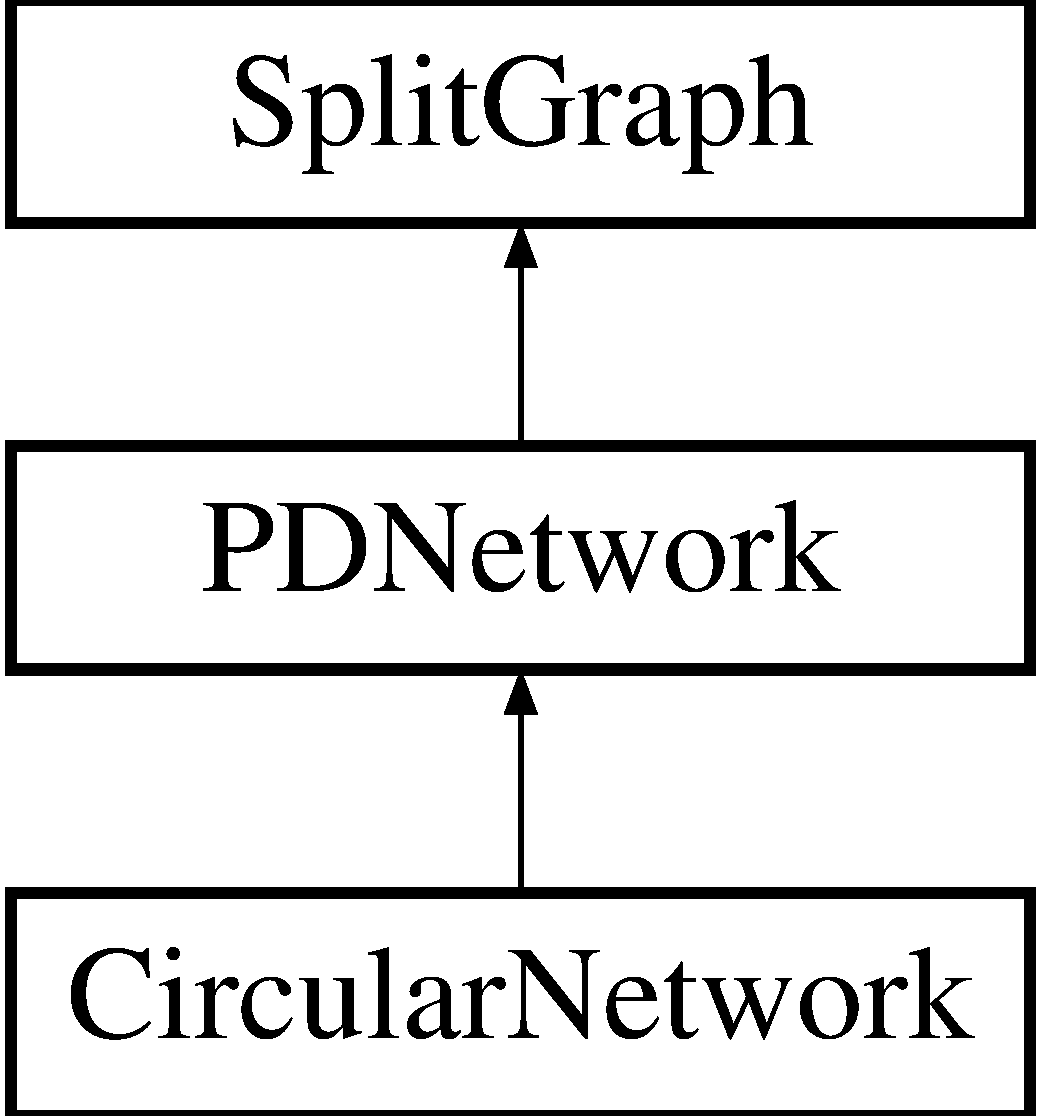
\includegraphics[height=3cm]{classPDNetwork}
\end{center}
\end{figure}
\subsection*{Public Member Functions}
\begin{DoxyCompactItemize}
\item 
\hyperlink{classPDNetwork_a26121c6a073dcaabb9c49e2b2144fde4}{PDNetwork} ()
\item 
\hyperlink{classPDNetwork_aba3316a0d0ed8fb67dce12fd9cc74b39}{PDNetwork} (\hyperlink{structParams}{Params} \&params)
\item 
void \hyperlink{classPDNetwork_a9a178e8280d5fc19f40b15903fc08320}{readRootNode} (const char $\ast$root\_\-name)
\item 
void \hyperlink{classPDNetwork_ab220164dcf5705a35884005476488262}{readParams} (\hyperlink{structParams}{Params} \&params)
\item 
void \hyperlink{classPDNetwork_ad228e5aa31704ab00b4689bcde67551c}{readInitialSet} (\hyperlink{structParams}{Params} \&params)
\item 
void \hyperlink{classPDNetwork_ad63b20eaa9bc56a456350d590f1c574e}{readInitialAreas} (\hyperlink{structParams}{Params} \&params)
\item 
void \hyperlink{classPDNetwork_a8612c1f67250fad10a5585ec727019ab}{proceedInitialSet} ()
\item 
void \hyperlink{classPDNetwork_ae7dc55bf1b3d05baa5ee85f58709ccc3}{initPDMin} ()
\item 
int \hyperlink{classPDNetwork_ad93961e85ba88b91ce1afce0ba594fa7}{calcCost} (IntVector \&taxset)
\item 
int \hyperlink{classPDNetwork_a14b0a52d17495905424fb42b81d61af3}{calcCost} (\hyperlink{classSplit}{Split} \&taxset)
\item 
void \hyperlink{classPDNetwork_a7a4584a81ad96405c27083bc436ab9ce}{computePD} (\hyperlink{structParams}{Params} \&params, \hyperlink{classSplitSet}{SplitSet} \&taxa\_\-set, \hyperlink{structPDRelatedMeasures}{PDRelatedMeasures} \&pd\_\-more)
\item 
virtual void \hyperlink{classPDNetwork_a43fb83d870d86c62c10e57e8eac7ecdd}{enterFindPD} (\hyperlink{structParams}{Params} \&params)
\item 
virtual void \hyperlink{classPDNetwork_ae481d52c7f411e1fa1f768746329130b}{findPD} (\hyperlink{structParams}{Params} \&params, vector$<$ \hyperlink{classSplitSet}{SplitSet} $>$ \&taxa\_\-set, vector$<$ int $>$ \&taxa\_\-order)
\item 
virtual void \hyperlink{classPDNetwork_a22260c3a934e8f657451066bb45d9ce2}{leaveFindPD} (vector$<$ \hyperlink{classSplitSet}{SplitSet} $>$ \&taxa\_\-set)
\item 
void \hyperlink{classPDNetwork_a49a2c3d1f88418aefe5c254cb1d54c03}{calcPDGain} (vector$<$ \hyperlink{classSplitSet}{SplitSet} $>$ \&pd\_\-set, matrix(double)\&delta)
\item 
void \hyperlink{classPDNetwork_a4921770ad17b4d871726b0f118386bcf}{calcPD} (\hyperlink{classSplit}{Split} \&id\_\-set)
\item 
void \hyperlink{classPDNetwork_ae591e54724f7d6f31b0b1ba264bfb876}{calcPDArea} (\hyperlink{classSplit}{Split} \&area\_\-id\_\-set)
\item 
void \hyperlink{classPDNetwork_a0500f181c9b5f1d42812794a7ece40c4}{calcExclusivePD} (\hyperlink{classSplit}{Split} \&id\_\-set)
\item 
void \hyperlink{classPDNetwork_ae578ebf3ba8d3dff2275b7961abd9574}{calcPDEndemism} (\hyperlink{classSplitSet}{SplitSet} \&area\_\-set, DoubleVector \&pd\_\-endem)
\item 
void \hyperlink{classPDNetwork_aff4ede123b2e4460a44d43fc504427ca}{calcPDComplementarity} (\hyperlink{classSplitSet}{SplitSet} \&area\_\-set, char $\ast$area\_\-names, vector$<$ \hyperlink{classNxsString}{NxsString} $>$ \&all\_\-names, DoubleVector \&pd\_\-comp)
\item 
void \hyperlink{classPDNetwork_aab6e6faf6c987ce8a4c5780b02774503}{transformLP} (\hyperlink{structParams}{Params} \&params, const char $\ast$outfile, int total\_\-size, bool make\_\-bin)
\item 
void \hyperlink{classPDNetwork_a0845b62f009a89057f045019dc547ff2}{transformLP\_\-Area} (\hyperlink{structParams}{Params} \&params, const char $\ast$outfile, int total\_\-size, bool make\_\-bin)
\item 
void \hyperlink{classPDNetwork_aa86d84304ea9865f0a97f1329057b6ad}{findPD\_\-LP} (\hyperlink{structParams}{Params} \&params, vector$<$ \hyperlink{classSplitSet}{SplitSet} $>$ \&taxa\_\-set)
\item 
void \hyperlink{classPDNetwork_ab7529ca69f5a56de23aae6853276dec7}{findPDArea\_\-LP} (\hyperlink{structParams}{Params} \&params, vector$<$ \hyperlink{classSplitSet}{SplitSet} $>$ \&areas\_\-set)
\item 
bool \hyperlink{classPDNetwork_a4b01aead98ff4ffc2f4ad1b020ffaa39}{isPDArea} ()
\item 
bool \hyperlink{classPDNetwork_aa7a36298000e66475cbd4f4ceab2f662}{checkAreaCoverage} ()
\item 
void \hyperlink{classPDNetwork_a02a5df18864c94bef7bbbfa0f5f7c80b}{transformLP\_\-Area\_\-Coverage} (const char $\ast$outfile, \hyperlink{classSplit}{Split} \&included\_\-area)
\item 
int \hyperlink{classPDNetwork_ad5c5c01afa0f14529d2b798670c8ce25}{findMinAreas} (\hyperlink{structParams}{Params} \&params, \hyperlink{classSplit}{Split} \&area\_\-id)
\end{DoxyCompactItemize}
\subsection*{Public Attributes}
\begin{DoxyCompactItemize}
\item 
\hyperlink{classSplitSet}{SplitSet} \hyperlink{classPDNetwork_a74a7b822f5483c3a6e2e6bbdc98ef1a3}{area\_\-taxa}
\end{DoxyCompactItemize}
\subsection*{Protected Member Functions}
\begin{DoxyCompactItemize}
\item 
int \hyperlink{classPDNetwork_af8e34bc2e3a369335ef9c7499a2712ea}{calcMaxBudget} ()
\item 
double \hyperlink{classPDNetwork_a45e8597bb2a7f8829b2560c613a10497}{greedyPD} (int subsize, \hyperlink{classSplit}{Split} \&taxa\_\-set, vector$<$ int $>$ \&taxa\_\-order)
\item 
double \hyperlink{classPDNetwork_afad7cba535aee59bb8b96542cb195e35}{localSearchPD} (int subsize, \hyperlink{classSplit}{Split} \&taxa\_\-set, vector$<$ int $>$ \&taxa\_\-order)
\item 
double \hyperlink{classPDNetwork_ac61874535f7ab2a49611444ca53b93cd}{exhaustPD2} (int subsize, int cur\_\-tax, \hyperlink{classSplit}{Split} \&curset, bool find\_\-all, \hyperlink{classSplitSet}{SplitSet} \&best\_\-set, vector$<$ int $>$ \&taxa\_\-order, IntList \&rem\_\-splits, IntList::iterator \&rem\_\-it)
\item 
double \hyperlink{classPDNetwork_a05d495099dac5a851aa057c05bd5f780}{exhaustPDBudget} (int cur\_\-budget, int cur\_\-tax, \hyperlink{classSplit}{Split} \&curset, bool find\_\-all, \hyperlink{classSplitSet}{SplitSet} \&best\_\-set, vector$<$ int $>$ \&taxa\_\-order, IntList \&rem\_\-splits, IntList::iterator \&rem\_\-it)
\item 
double \hyperlink{classPDNetwork_adbdf5778b7d6b1468d9a32c831d0f951}{calcRaisedWeight} (\hyperlink{classSplit}{Split} \&taxa\_\-set, IntList \&rem\_\-splits, IntList::iterator \&rem\_\-it)
\item 
void \hyperlink{classPDNetwork_a684fdd0cfd902a037bb8ce0bb6846a43}{updateSplitVector} (\hyperlink{classSplit}{Split} \&curset, \hyperlink{classSplitSet}{SplitSet} \&best\_\-set)
\item 
void \hyperlink{classPDNetwork_a1e9909731a5f229897392d802ef69a60}{checkYValue} (int total\_\-size, vector$<$ int $>$ \&y\_\-value)
\item 
void \hyperlink{classPDNetwork_a438360816421d31dc8902323ce57a497}{checkYValue\_\-Area} (int total\_\-size, vector$<$ int $>$ \&y\_\-value, vector$<$ int $>$ \&count1, vector$<$ int $>$ \&count2)
\item 
bool \hyperlink{classPDNetwork_a89a41e4b180dacd776a0496cb4137080}{isUniquelyCovered} (int taxon, int \&area)
\end{DoxyCompactItemize}
\subsection*{Protected Attributes}
\begin{DoxyCompactItemize}
\item 
double \hyperlink{classPDNetwork_a0a092e4f0267eb88e6459e9e7e552b14}{extra\_\-pd}
\item 
bool \hyperlink{classPDNetwork_a2427fd91e8ae19784de05e574ea75dae}{min\_\-pd}
\item 
IntVector \hyperlink{classPDNetwork_a316ec40bb65670852e08371985d786e0}{initialset}
\item 
IntVector \hyperlink{classPDNetwork_ae82636a4b7ce25ca1604cceefc79bb6a}{initialareas}
\end{DoxyCompactItemize}
\subsection*{Friends}
\begin{DoxyCompactItemize}
\item 
\hypertarget{classPDNetwork_a7a747beac427dfc013c53501e474d452}{
class \hyperlink{classPDNetwork_a7a747beac427dfc013c53501e474d452}{MTree}}
\label{classPDNetwork_a7a747beac427dfc013c53501e474d452}

\end{DoxyCompactItemize}


\subsection{Detailed Description}
General \hyperlink{classSplit}{Split} Network for Phylogenetic Diversity Algorithm

\begin{DoxyAuthor}{Author}
BUI Quang Minh, Steffen Klaere, Arndt von Haeseler 
\end{DoxyAuthor}


\subsection{Constructor \& Destructor Documentation}
\hypertarget{classPDNetwork_a26121c6a073dcaabb9c49e2b2144fde4}{
\index{PDNetwork@{PDNetwork}!PDNetwork@{PDNetwork}}
\index{PDNetwork@{PDNetwork}!PDNetwork@{PDNetwork}}
\subsubsection[{PDNetwork}]{\setlength{\rightskip}{0pt plus 5cm}PDNetwork::PDNetwork ()}}
\label{classPDNetwork_a26121c6a073dcaabb9c49e2b2144fde4}
empty constructor \hypertarget{classPDNetwork_aba3316a0d0ed8fb67dce12fd9cc74b39}{
\index{PDNetwork@{PDNetwork}!PDNetwork@{PDNetwork}}
\index{PDNetwork@{PDNetwork}!PDNetwork@{PDNetwork}}
\subsubsection[{PDNetwork}]{\setlength{\rightskip}{0pt plus 5cm}PDNetwork::PDNetwork ({\bf Params} \& {\em params})}}
\label{classPDNetwork_aba3316a0d0ed8fb67dce12fd9cc74b39}
construct PD network from a NEXUS or NEWICK file, e.g. produced by SplitsTree 
\begin{DoxyParams}{Parameters}
\item[{\em params}]program parameters \end{DoxyParams}


\subsection{Member Function Documentation}
\hypertarget{classPDNetwork_a14b0a52d17495905424fb42b81d61af3}{
\index{PDNetwork@{PDNetwork}!calcCost@{calcCost}}
\index{calcCost@{calcCost}!PDNetwork@{PDNetwork}}
\subsubsection[{calcCost}]{\setlength{\rightskip}{0pt plus 5cm}int PDNetwork::calcCost ({\bf Split} \& {\em taxset})}}
\label{classPDNetwork_a14b0a52d17495905424fb42b81d61af3}
compute the minimum required costs to conserve a taxa set 
\begin{DoxyParams}{Parameters}
\item[{\em taxset}]set of taxa \end{DoxyParams}
\begin{DoxyReturn}{Returns}
budget required
\end{DoxyReturn}
compute the required costs to conserve a taxa set 
\begin{DoxyParams}{Parameters}
\item[{\em taxset}]set of taxa \end{DoxyParams}
\begin{DoxyReturn}{Returns}
minimum budget required 
\end{DoxyReturn}
\hypertarget{classPDNetwork_ad93961e85ba88b91ce1afce0ba594fa7}{
\index{PDNetwork@{PDNetwork}!calcCost@{calcCost}}
\index{calcCost@{calcCost}!PDNetwork@{PDNetwork}}
\subsubsection[{calcCost}]{\setlength{\rightskip}{0pt plus 5cm}int PDNetwork::calcCost (IntVector \& {\em taxset})}}
\label{classPDNetwork_ad93961e85ba88b91ce1afce0ba594fa7}
compute the minimum required costs to conserve a taxa set 
\begin{DoxyParams}{Parameters}
\item[{\em taxset}]set of taxa \end{DoxyParams}
\begin{DoxyReturn}{Returns}
budget required
\end{DoxyReturn}
compute the required costs to conserve a taxa set 
\begin{DoxyParams}{Parameters}
\item[{\em taxset}]set of taxa \end{DoxyParams}
\begin{DoxyReturn}{Returns}
minimum budget required 
\end{DoxyReturn}
\hypertarget{classPDNetwork_a0500f181c9b5f1d42812794a7ece40c4}{
\index{PDNetwork@{PDNetwork}!calcExclusivePD@{calcExclusivePD}}
\index{calcExclusivePD@{calcExclusivePD}!PDNetwork@{PDNetwork}}
\subsubsection[{calcExclusivePD}]{\setlength{\rightskip}{0pt plus 5cm}void PDNetwork::calcExclusivePD ({\bf Split} \& {\em id\_\-set})}}
\label{classPDNetwork_a0500f181c9b5f1d42812794a7ece40c4}
compute the EXCLUSIVE PD score of a given taxa set with name in taxa\_\-name, result is written to id\_\-set.weight 
\begin{DoxyParams}{Parameters}
\item[{\em id\_\-set}](IN/OUT) corresponding set of taxa IDs \end{DoxyParams}
\hypertarget{classPDNetwork_af8e34bc2e3a369335ef9c7499a2712ea}{
\index{PDNetwork@{PDNetwork}!calcMaxBudget@{calcMaxBudget}}
\index{calcMaxBudget@{calcMaxBudget}!PDNetwork@{PDNetwork}}
\subsubsection[{calcMaxBudget}]{\setlength{\rightskip}{0pt plus 5cm}int PDNetwork::calcMaxBudget ()\hspace{0.3cm}{\ttfamily  \mbox{[}protected\mbox{]}}}}
\label{classPDNetwork_af8e34bc2e3a369335ef9c7499a2712ea}
calculate the total maximum budget required \begin{DoxyReturn}{Returns}
total maximum budget required 
\end{DoxyReturn}
\hypertarget{classPDNetwork_a4921770ad17b4d871726b0f118386bcf}{
\index{PDNetwork@{PDNetwork}!calcPD@{calcPD}}
\index{calcPD@{calcPD}!PDNetwork@{PDNetwork}}
\subsubsection[{calcPD}]{\setlength{\rightskip}{0pt plus 5cm}void PDNetwork::calcPD ({\bf Split} \& {\em id\_\-set})}}
\label{classPDNetwork_a4921770ad17b4d871726b0f118386bcf}
compute the PD score of a given taxa set with name in taxa\_\-name, result is written to id\_\-set.weight. The difference from \hyperlink{classSplitGraph_aaff18dd254098b4e1912593f0e2de524}{calcWeight()} is that calcPD takes initialset into account 
\begin{DoxyParams}{Parameters}
\item[{\em id\_\-set}](IN/OUT) corresponding set of taxa \end{DoxyParams}
\hypertarget{classPDNetwork_ae591e54724f7d6f31b0b1ba264bfb876}{
\index{PDNetwork@{PDNetwork}!calcPDArea@{calcPDArea}}
\index{calcPDArea@{calcPDArea}!PDNetwork@{PDNetwork}}
\subsubsection[{calcPDArea}]{\setlength{\rightskip}{0pt plus 5cm}void PDNetwork::calcPDArea ({\bf Split} \& {\em area\_\-id\_\-set})}}
\label{classPDNetwork_ae591e54724f7d6f31b0b1ba264bfb876}
compute PD of a set of areas. It implicitly takes area\_\-taxa map into account. 
\begin{DoxyParams}{Parameters}
\item[{\em area\_\-id\_\-set}]IDs of areas in the set \end{DoxyParams}
\hypertarget{classPDNetwork_aff4ede123b2e4460a44d43fc504427ca}{
\index{PDNetwork@{PDNetwork}!calcPDComplementarity@{calcPDComplementarity}}
\index{calcPDComplementarity@{calcPDComplementarity}!PDNetwork@{PDNetwork}}
\subsubsection[{calcPDComplementarity}]{\setlength{\rightskip}{0pt plus 5cm}void PDNetwork::calcPDComplementarity ({\bf SplitSet} \& {\em area\_\-set}, \/  char $\ast$ {\em area\_\-names}, \/  vector$<$ {\bf NxsString} $>$ \& {\em all\_\-names}, \/  DoubleVector \& {\em pd\_\-comp})}}
\label{classPDNetwork_aff4ede123b2e4460a44d43fc504427ca}
compute the area's PD complementarity given a specific area 
\begin{DoxyParams}{Parameters}
\item[{\em area\_\-set}]set of area \item[{\em area\_\-names}]given area names as string separated by commas \item[{\em all\_\-names}]all area names \item[{\em pd\_\-comp}](OUT) corresponding PD endemism \end{DoxyParams}
\hypertarget{classPDNetwork_ae578ebf3ba8d3dff2275b7961abd9574}{
\index{PDNetwork@{PDNetwork}!calcPDEndemism@{calcPDEndemism}}
\index{calcPDEndemism@{calcPDEndemism}!PDNetwork@{PDNetwork}}
\subsubsection[{calcPDEndemism}]{\setlength{\rightskip}{0pt plus 5cm}void PDNetwork::calcPDEndemism ({\bf SplitSet} \& {\em area\_\-set}, \/  DoubleVector \& {\em pd\_\-endem})}}
\label{classPDNetwork_ae578ebf3ba8d3dff2275b7961abd9574}
compute the area's PD ENDEMISM of set of area 
\begin{DoxyParams}{Parameters}
\item[{\em area\_\-set}]set of area \item[{\em pd\_\-endem}](OUT) corresponding PD endemism \end{DoxyParams}
\hypertarget{classPDNetwork_a49a2c3d1f88418aefe5c254cb1d54c03}{
\index{PDNetwork@{PDNetwork}!calcPDGain@{calcPDGain}}
\index{calcPDGain@{calcPDGain}!PDNetwork@{PDNetwork}}
\subsubsection[{calcPDGain}]{\setlength{\rightskip}{0pt plus 5cm}void PDNetwork::calcPDGain (vector$<$ {\bf SplitSet} $>$ \& {\em pd\_\-set}, \/  matrix(double)\& {\em delta})}}
\label{classPDNetwork_a49a2c3d1f88418aefe5c254cb1d54c03}
calculate the PD gain matrix in terms of delta\_\-k$^\wedge$j = pd(PD\_\-k $\backslash$/ \{j\}) -\/ pd\_\-k 
\begin{DoxyParams}{Parameters}
\item[{\em pd\_\-set}]set of optimal PD sets \item[{\em delta}](OUT) PD gain matrix \end{DoxyParams}
\hypertarget{classPDNetwork_adbdf5778b7d6b1468d9a32c831d0f951}{
\index{PDNetwork@{PDNetwork}!calcRaisedWeight@{calcRaisedWeight}}
\index{calcRaisedWeight@{calcRaisedWeight}!PDNetwork@{PDNetwork}}
\subsubsection[{calcRaisedWeight}]{\setlength{\rightskip}{0pt plus 5cm}double PDNetwork::calcRaisedWeight ({\bf Split} \& {\em taxa\_\-set}, \/  IntList \& {\em rem\_\-splits}, \/  IntList::iterator \& {\em rem\_\-it})\hspace{0.3cm}{\ttfamily  \mbox{[}protected\mbox{]}}}}
\label{classPDNetwork_adbdf5778b7d6b1468d9a32c831d0f951}
calculate sum of weights of preserved splits in the taxa\_\-set 
\begin{DoxyParams}{Parameters}
\item[{\em taxa\_\-set}]a set of taxa \item[{\em rem\_\-splits}]remaining splits \item[{\em rem\_\-it}]begin iterator of remaining splits\end{DoxyParams}
calculate sum of weights of preserved splits in the taxa\_\-set 
\begin{DoxyParams}{Parameters}
\item[{\em taxa\_\-set}]a set of taxa \end{DoxyParams}
\hypertarget{classPDNetwork_aa7a36298000e66475cbd4f4ceab2f662}{
\index{PDNetwork@{PDNetwork}!checkAreaCoverage@{checkAreaCoverage}}
\index{checkAreaCoverage@{checkAreaCoverage}!PDNetwork@{PDNetwork}}
\subsubsection[{checkAreaCoverage}]{\setlength{\rightskip}{0pt plus 5cm}bool PDNetwork::checkAreaCoverage ()}}
\label{classPDNetwork_aa7a36298000e66475cbd4f4ceab2f662}
check if all taxa are covered by the set of areas \begin{DoxyReturn}{Returns}
false if there exists some taxon which is not covered by any areas 
\end{DoxyReturn}
\hypertarget{classPDNetwork_a1e9909731a5f229897392d802ef69a60}{
\index{PDNetwork@{PDNetwork}!checkYValue@{checkYValue}}
\index{checkYValue@{checkYValue}!PDNetwork@{PDNetwork}}
\subsubsection[{checkYValue}]{\setlength{\rightskip}{0pt plus 5cm}void PDNetwork::checkYValue (int {\em total\_\-size}, \/  vector$<$ int $>$ \& {\em y\_\-value})\hspace{0.3cm}{\ttfamily  \mbox{[}protected\mbox{]}}}}
\label{classPDNetwork_a1e9909731a5f229897392d802ef69a60}
y variables in the LP formulation, check if it can be dropped or equals some x variable. 
\begin{DoxyParams}{Parameters}
\item[{\em total\_\-size}]k for PD\_\-k or total budget \item[{\em y\_\-value}](OUT): vector of: -\/1 if cannot reduce, 1 if equals 1, or id+2 where id is the trivial split id \end{DoxyParams}
\hypertarget{classPDNetwork_a438360816421d31dc8902323ce57a497}{
\index{PDNetwork@{PDNetwork}!checkYValue\_\-Area@{checkYValue\_\-Area}}
\index{checkYValue\_\-Area@{checkYValue\_\-Area}!PDNetwork@{PDNetwork}}
\subsubsection[{checkYValue\_\-Area}]{\setlength{\rightskip}{0pt plus 5cm}void PDNetwork::checkYValue\_\-Area (int {\em total\_\-size}, \/  vector$<$ int $>$ \& {\em y\_\-value}, \/  vector$<$ int $>$ \& {\em count1}, \/  vector$<$ int $>$ \& {\em count2})\hspace{0.3cm}{\ttfamily  \mbox{[}protected\mbox{]}}}}
\label{classPDNetwork_a438360816421d31dc8902323ce57a497}
y variables in the LP formulation for PD area optimization, check if it can be dropped or equals some x variable. 
\begin{DoxyParams}{Parameters}
\item[{\em total\_\-size}]k for PD\_\-k or total budget \item[{\em y\_\-value}](OUT) vector of: -\/1 if cannot reduce, 1 if can be dropped, or id+2 where id is the trivial area id \item[{\em count1}](OUT) count of x variables in the inequality 1 \item[{\em count2}](OUT) count of x variables in the inequality 2 \end{DoxyParams}
\hypertarget{classPDNetwork_a7a4584a81ad96405c27083bc436ab9ce}{
\index{PDNetwork@{PDNetwork}!computePD@{computePD}}
\index{computePD@{computePD}!PDNetwork@{PDNetwork}}
\subsubsection[{computePD}]{\setlength{\rightskip}{0pt plus 5cm}void PDNetwork::computePD ({\bf Params} \& {\em params}, \/  {\bf SplitSet} \& {\em taxa\_\-set}, \/  {\bf PDRelatedMeasures} \& {\em pd\_\-more})}}
\label{classPDNetwork_a7a4584a81ad96405c27083bc436ab9ce}
compute the PD score of a given taxa set in filename 
\begin{DoxyParams}{Parameters}
\item[{\em params}]program parameters \item[{\em taxa\_\-set}](OUT) corresponding set of taxa \item[{\em pd\_\-more}](OUT) more computed PD measures will be stored here \end{DoxyParams}
\hypertarget{classPDNetwork_a43fb83d870d86c62c10e57e8eac7ecdd}{
\index{PDNetwork@{PDNetwork}!enterFindPD@{enterFindPD}}
\index{enterFindPD@{enterFindPD}!PDNetwork@{PDNetwork}}
\subsubsection[{enterFindPD}]{\setlength{\rightskip}{0pt plus 5cm}void PDNetwork::enterFindPD ({\bf Params} \& {\em params})\hspace{0.3cm}{\ttfamily  \mbox{[}virtual\mbox{]}}}}
\label{classPDNetwork_a43fb83d870d86c62c10e57e8eac7ecdd}
this will be called by findPD at the beginning 
\begin{DoxyParams}{Parameters}
\item[{\em params}]program parameters \end{DoxyParams}
\hypertarget{classPDNetwork_ac61874535f7ab2a49611444ca53b93cd}{
\index{PDNetwork@{PDNetwork}!exhaustPD2@{exhaustPD2}}
\index{exhaustPD2@{exhaustPD2}!PDNetwork@{PDNetwork}}
\subsubsection[{exhaustPD2}]{\setlength{\rightskip}{0pt plus 5cm}double PDNetwork::exhaustPD2 (int {\em subsize}, \/  int {\em cur\_\-tax}, \/  {\bf Split} \& {\em curset}, \/  bool {\em find\_\-all}, \/  {\bf SplitSet} \& {\em best\_\-set}, \/  vector$<$ int $>$ \& {\em taxa\_\-order}, \/  IntList \& {\em rem\_\-splits}, \/  IntList::iterator \& {\em rem\_\-it})\hspace{0.3cm}{\ttfamily  \mbox{[}protected\mbox{]}}}}
\label{classPDNetwork_ac61874535f7ab2a49611444ca53b93cd}
exhaustive search version 2 for maximal phylogenetic diversity of a given size 
\begin{DoxyParams}{Parameters}
\item[{\em subsize}]the subset size \item[{\em cur\_\-tax}]current taxon \item[{\em curset}]current set \item[{\em find\_\-all}]TRUE if wanting all max PD set \item[{\em best\_\-set}](OUT) the set of taxa in the maximal PD set \item[{\em taxa\_\-order}](OUT) order of inserted taxa \item[{\em rem\_\-splits}](IN) remaining splits \item[{\em rem\_\-it}](IN) begin of remaining iterator \end{DoxyParams}
\begin{DoxyReturn}{Returns}
the PD score of the maximal set
\end{DoxyReturn}
exhaustive search VERSION 2 for maximal phylogenetic diversity of a given size 
\begin{DoxyParams}{Parameters}
\item[{\em subsize}]the subset size \item[{\em best\_\-set}](OUT) the set of taxa in the maximal PD set \item[{\em cur\_\-tax}]current taxon \item[{\em curset}]current set \item[{\em taxa\_\-order}](OUT) order of inserted taxa \item[{\em rem\_\-splits}](IN) remaining splits \end{DoxyParams}
\begin{DoxyReturn}{Returns}
the PD score of the maximal set 
\end{DoxyReturn}
\hypertarget{classPDNetwork_a05d495099dac5a851aa057c05bd5f780}{
\index{PDNetwork@{PDNetwork}!exhaustPDBudget@{exhaustPDBudget}}
\index{exhaustPDBudget@{exhaustPDBudget}!PDNetwork@{PDNetwork}}
\subsubsection[{exhaustPDBudget}]{\setlength{\rightskip}{0pt plus 5cm}double PDNetwork::exhaustPDBudget (int {\em cur\_\-budget}, \/  int {\em cur\_\-tax}, \/  {\bf Split} \& {\em curset}, \/  bool {\em find\_\-all}, \/  {\bf SplitSet} \& {\em best\_\-set}, \/  vector$<$ int $>$ \& {\em taxa\_\-order}, \/  IntList \& {\em rem\_\-splits}, \/  IntList::iterator \& {\em rem\_\-it})\hspace{0.3cm}{\ttfamily  \mbox{[}protected\mbox{]}}}}
\label{classPDNetwork_a05d495099dac5a851aa057c05bd5f780}
exhaustive search for maximal PD with cost-\/constrained 
\begin{DoxyParams}{Parameters}
\item[{\em cur\_\-budget}]current budget \item[{\em cur\_\-tax}]current taxon \item[{\em curset}]current set \item[{\em find\_\-all}]TRUE if wanting all max PD set \item[{\em best\_\-set}](OUT) the set of taxa in the maximal PD set \item[{\em taxa\_\-order}](OUT) order of inserted taxa \item[{\em rem\_\-splits}](IN) remaining splits \item[{\em rem\_\-it}](IN) begin of remaining iterator \end{DoxyParams}
\begin{DoxyReturn}{Returns}
the PD score of the maximal set 
\end{DoxyReturn}
\hypertarget{classPDNetwork_ad5c5c01afa0f14529d2b798670c8ce25}{
\index{PDNetwork@{PDNetwork}!findMinAreas@{findMinAreas}}
\index{findMinAreas@{findMinAreas}!PDNetwork@{PDNetwork}}
\subsubsection[{findMinAreas}]{\setlength{\rightskip}{0pt plus 5cm}int PDNetwork::findMinAreas ({\bf Params} \& {\em params}, \/  {\bf Split} \& {\em area\_\-id})}}
\label{classPDNetwork_ad5c5c01afa0f14529d2b798670c8ce25}
\begin{DoxyReturn}{Returns}
the minimum number of areas needed to cover all taxa 
\end{DoxyReturn}

\begin{DoxyParams}{Parameters}
\item[{\em params}]program parameters \item[{\em area\_\-id}](OUT) minimal set of areas which cover all taxa \end{DoxyParams}
\hypertarget{classPDNetwork_ae481d52c7f411e1fa1f768746329130b}{
\index{PDNetwork@{PDNetwork}!findPD@{findPD}}
\index{findPD@{findPD}!PDNetwork@{PDNetwork}}
\subsubsection[{findPD}]{\setlength{\rightskip}{0pt plus 5cm}void PDNetwork::findPD ({\bf Params} \& {\em params}, \/  vector$<$ {\bf SplitSet} $>$ \& {\em taxa\_\-set}, \/  vector$<$ int $>$ \& {\em taxa\_\-order})\hspace{0.3cm}{\ttfamily  \mbox{[}virtual\mbox{]}}}}
\label{classPDNetwork_ae481d52c7f411e1fa1f768746329130b}
main function to search for maximal phylogenetic diversity 
\begin{DoxyParams}{Parameters}
\item[{\em params}]program parameters \item[{\em taxa\_\-set}](OUT) the vector of set of taxa in the maximal PD set \item[{\em taxa\_\-order}](OUT) order of inserted taxa \end{DoxyParams}


Reimplemented in \hyperlink{classCircularNetwork_a2d7a229ba82a87667c7f194249484f38}{CircularNetwork}.\hypertarget{classPDNetwork_aa86d84304ea9865f0a97f1329057b6ad}{
\index{PDNetwork@{PDNetwork}!findPD\_\-LP@{findPD\_\-LP}}
\index{findPD\_\-LP@{findPD\_\-LP}!PDNetwork@{PDNetwork}}
\subsubsection[{findPD\_\-LP}]{\setlength{\rightskip}{0pt plus 5cm}void PDNetwork::findPD\_\-LP ({\bf Params} \& {\em params}, \/  vector$<$ {\bf SplitSet} $>$ \& {\em taxa\_\-set})}}
\label{classPDNetwork_aa86d84304ea9865f0a97f1329057b6ad}
transform the PD problem into linear programming and solve it 
\begin{DoxyParams}{Parameters}
\item[{\em params}]program parameters \item[{\em taxa\_\-set}](OUT) the vector of set of taxa in the maximal PD set \end{DoxyParams}
\hypertarget{classPDNetwork_ab7529ca69f5a56de23aae6853276dec7}{
\index{PDNetwork@{PDNetwork}!findPDArea\_\-LP@{findPDArea\_\-LP}}
\index{findPDArea\_\-LP@{findPDArea\_\-LP}!PDNetwork@{PDNetwork}}
\subsubsection[{findPDArea\_\-LP}]{\setlength{\rightskip}{0pt plus 5cm}void PDNetwork::findPDArea\_\-LP ({\bf Params} \& {\em params}, \/  vector$<$ {\bf SplitSet} $>$ \& {\em areas\_\-set})}}
\label{classPDNetwork_ab7529ca69f5a56de23aae6853276dec7}
transform the PD problem into linear programming and solve it 
\begin{DoxyParams}{Parameters}
\item[{\em params}]program parameters \item[{\em areas\_\-set}](OUT) the vector of set of areas in the maximal PD set \end{DoxyParams}
\hypertarget{classPDNetwork_a45e8597bb2a7f8829b2560c613a10497}{
\index{PDNetwork@{PDNetwork}!greedyPD@{greedyPD}}
\index{greedyPD@{greedyPD}!PDNetwork@{PDNetwork}}
\subsubsection[{greedyPD}]{\setlength{\rightskip}{0pt plus 5cm}double PDNetwork::greedyPD (int {\em subsize}, \/  {\bf Split} \& {\em taxa\_\-set}, \/  vector$<$ int $>$ \& {\em taxa\_\-order})\hspace{0.3cm}{\ttfamily  \mbox{[}protected\mbox{]}}}}
\label{classPDNetwork_a45e8597bb2a7f8829b2560c613a10497}
greedy algorithm for phylogenetic diversity of a given size 
\begin{DoxyParams}{Parameters}
\item[{\em subsize}]the subset size \item[{\em taxa\_\-set}](OUT) the set of taxa in the PD-\/set \item[{\em taxa\_\-order}](OUT) order of inserted taxa \end{DoxyParams}
\begin{DoxyReturn}{Returns}
the PD score of the maximal set, also returned in taxa\_\-set.weight
\end{DoxyReturn}
greedy algorithm for phylogenetic diversity of a given size 
\begin{DoxyParams}{Parameters}
\item[{\em subsize}]the subset size \item[{\em taxa\_\-set}](OUT) the set of taxa in the PD-\/set \end{DoxyParams}
\begin{DoxyReturn}{Returns}
the PD score of the maximal set, also returned in taxa\_\-set.weight 
\end{DoxyReturn}
\hypertarget{classPDNetwork_ae7dc55bf1b3d05baa5ee85f58709ccc3}{
\index{PDNetwork@{PDNetwork}!initPDMin@{initPDMin}}
\index{initPDMin@{initPDMin}!PDNetwork@{PDNetwork}}
\subsubsection[{initPDMin}]{\setlength{\rightskip}{0pt plus 5cm}void PDNetwork::initPDMin ()}}
\label{classPDNetwork_ae7dc55bf1b3d05baa5ee85f58709ccc3}
initialize when PD min specified \hypertarget{classPDNetwork_a4b01aead98ff4ffc2f4ad1b020ffaa39}{
\index{PDNetwork@{PDNetwork}!isPDArea@{isPDArea}}
\index{isPDArea@{isPDArea}!PDNetwork@{PDNetwork}}
\subsubsection[{isPDArea}]{\setlength{\rightskip}{0pt plus 5cm}bool PDNetwork::isPDArea ()}}
\label{classPDNetwork_a4b01aead98ff4ffc2f4ad1b020ffaa39}
\begin{DoxyReturn}{Returns}
TRUE if we are doing PD area optimization 
\end{DoxyReturn}
\hypertarget{classPDNetwork_a89a41e4b180dacd776a0496cb4137080}{
\index{PDNetwork@{PDNetwork}!isUniquelyCovered@{isUniquelyCovered}}
\index{isUniquelyCovered@{isUniquelyCovered}!PDNetwork@{PDNetwork}}
\subsubsection[{isUniquelyCovered}]{\setlength{\rightskip}{0pt plus 5cm}bool PDNetwork::isUniquelyCovered (int {\em taxon}, \/  int \& {\em area})\hspace{0.3cm}{\ttfamily  \mbox{[}protected\mbox{]}}}}
\label{classPDNetwork_a89a41e4b180dacd776a0496cb4137080}
check if a taxon is uniquely covered by one area 
\begin{DoxyParams}{Parameters}
\item[{\em taxon}]the taxon ID \item[{\em area}](OUT) area the area ID that covers taxon \end{DoxyParams}
\begin{DoxyReturn}{Returns}
TRUE if the 'taxon' is uniquely covered by only one area. Otherwise FALSE. 
\end{DoxyReturn}
\hypertarget{classPDNetwork_a22260c3a934e8f657451066bb45d9ce2}{
\index{PDNetwork@{PDNetwork}!leaveFindPD@{leaveFindPD}}
\index{leaveFindPD@{leaveFindPD}!PDNetwork@{PDNetwork}}
\subsubsection[{leaveFindPD}]{\setlength{\rightskip}{0pt plus 5cm}void PDNetwork::leaveFindPD (vector$<$ {\bf SplitSet} $>$ \& {\em taxa\_\-set})\hspace{0.3cm}{\ttfamily  \mbox{[}virtual\mbox{]}}}}
\label{classPDNetwork_a22260c3a934e8f657451066bb45d9ce2}
this function will be called by findPD at the end 
\begin{DoxyParams}{Parameters}
\item[{\em taxa\_\-set}](IN/OUT) the vector of set of taxa in the maximal PD set \end{DoxyParams}
\hypertarget{classPDNetwork_afad7cba535aee59bb8b96542cb195e35}{
\index{PDNetwork@{PDNetwork}!localSearchPD@{localSearchPD}}
\index{localSearchPD@{localSearchPD}!PDNetwork@{PDNetwork}}
\subsubsection[{localSearchPD}]{\setlength{\rightskip}{0pt plus 5cm}double PDNetwork::localSearchPD (int {\em subsize}, \/  {\bf Split} \& {\em taxa\_\-set}, \/  vector$<$ int $>$ \& {\em taxa\_\-order})\hspace{0.3cm}{\ttfamily  \mbox{[}protected\mbox{]}}}}
\label{classPDNetwork_afad7cba535aee59bb8b96542cb195e35}
local search algorithm for phylogenetic diversity of a given size 
\begin{DoxyParams}{Parameters}
\item[{\em subsize}]the subset size \item[{\em taxa\_\-set}](OUT) the set of taxa in the PD-\/set \item[{\em taxa\_\-order}](IN) order of inserted taxa \end{DoxyParams}
\begin{DoxyReturn}{Returns}
the PD score of the maximal set, also returned in taxa\_\-set.weight
\end{DoxyReturn}
testing algorithm for phylogenetic diversity of a given size 
\begin{DoxyParams}{Parameters}
\item[{\em subsize}]the subset size \item[{\em taxa\_\-set}](OUT) the set of taxa in the PD-\/set \end{DoxyParams}
\begin{DoxyReturn}{Returns}
the PD score of the maximal set, also returned in taxa\_\-set.weight 
\end{DoxyReturn}
\hypertarget{classPDNetwork_a8612c1f67250fad10a5585ec727019ab}{
\index{PDNetwork@{PDNetwork}!proceedInitialSet@{proceedInitialSet}}
\index{proceedInitialSet@{proceedInitialSet}!PDNetwork@{PDNetwork}}
\subsubsection[{proceedInitialSet}]{\setlength{\rightskip}{0pt plus 5cm}void PDNetwork::proceedInitialSet ()}}
\label{classPDNetwork_a8612c1f67250fad10a5585ec727019ab}
increase the weight of the split associated with initial set \hypertarget{classPDNetwork_ad63b20eaa9bc56a456350d590f1c574e}{
\index{PDNetwork@{PDNetwork}!readInitialAreas@{readInitialAreas}}
\index{readInitialAreas@{readInitialAreas}!PDNetwork@{PDNetwork}}
\subsubsection[{readInitialAreas}]{\setlength{\rightskip}{0pt plus 5cm}void PDNetwork::readInitialAreas ({\bf Params} \& {\em params})}}
\label{classPDNetwork_ad63b20eaa9bc56a456350d590f1c574e}
read the initial areas to be included into PD set 
\begin{DoxyParams}{Parameters}
\item[{\em params}]program parameters \end{DoxyParams}
\hypertarget{classPDNetwork_ad228e5aa31704ab00b4689bcde67551c}{
\index{PDNetwork@{PDNetwork}!readInitialSet@{readInitialSet}}
\index{readInitialSet@{readInitialSet}!PDNetwork@{PDNetwork}}
\subsubsection[{readInitialSet}]{\setlength{\rightskip}{0pt plus 5cm}void PDNetwork::readInitialSet ({\bf Params} \& {\em params})}}
\label{classPDNetwork_ad228e5aa31704ab00b4689bcde67551c}
read the initial set of taxa to be included into PD-\/tree 
\begin{DoxyParams}{Parameters}
\item[{\em params}]program parameters \end{DoxyParams}
\hypertarget{classPDNetwork_ab220164dcf5705a35884005476488262}{
\index{PDNetwork@{PDNetwork}!readParams@{readParams}}
\index{readParams@{readParams}!PDNetwork@{PDNetwork}}
\subsubsection[{readParams}]{\setlength{\rightskip}{0pt plus 5cm}void PDNetwork::readParams ({\bf Params} \& {\em params})}}
\label{classPDNetwork_ab220164dcf5705a35884005476488262}
read the parameter from the file and incoporate into split system 
\begin{DoxyParams}{Parameters}
\item[{\em params}]program parameters \end{DoxyParams}
\hypertarget{classPDNetwork_a9a178e8280d5fc19f40b15903fc08320}{
\index{PDNetwork@{PDNetwork}!readRootNode@{readRootNode}}
\index{readRootNode@{readRootNode}!PDNetwork@{PDNetwork}}
\subsubsection[{readRootNode}]{\setlength{\rightskip}{0pt plus 5cm}void PDNetwork::readRootNode (const char $\ast$ {\em root\_\-name})}}
\label{classPDNetwork_a9a178e8280d5fc19f40b15903fc08320}
Identify the root node if specified, include it into the initial set 
\begin{DoxyParams}{Parameters}
\item[{\em root\_\-name}]name of the root node \end{DoxyParams}
\hypertarget{classPDNetwork_aab6e6faf6c987ce8a4c5780b02774503}{
\index{PDNetwork@{PDNetwork}!transformLP@{transformLP}}
\index{transformLP@{transformLP}!PDNetwork@{PDNetwork}}
\subsubsection[{transformLP}]{\setlength{\rightskip}{0pt plus 5cm}void PDNetwork::transformLP ({\bf Params} \& {\em params}, \/  const char $\ast$ {\em outfile}, \/  int {\em total\_\-size}, \/  bool {\em make\_\-bin})}}
\label{classPDNetwork_aab6e6faf6c987ce8a4c5780b02774503}
transform the problem into an Integer Linear Programming and write to .lp file 
\begin{DoxyParams}{Parameters}
\item[{\em params}]program parameters \item[{\em outfile}]name of output file in LP format \item[{\em total\_\-size}]k for PD\_\-k or total budget \item[{\em make\_\-bin}]TRUE if creating binary programming \end{DoxyParams}
\hypertarget{classPDNetwork_a0845b62f009a89057f045019dc547ff2}{
\index{PDNetwork@{PDNetwork}!transformLP\_\-Area@{transformLP\_\-Area}}
\index{transformLP\_\-Area@{transformLP\_\-Area}!PDNetwork@{PDNetwork}}
\subsubsection[{transformLP\_\-Area}]{\setlength{\rightskip}{0pt plus 5cm}void PDNetwork::transformLP\_\-Area ({\bf Params} \& {\em params}, \/  const char $\ast$ {\em outfile}, \/  int {\em total\_\-size}, \/  bool {\em make\_\-bin})}}
\label{classPDNetwork_a0845b62f009a89057f045019dc547ff2}
transform the problem into an Integer Linear Programming and write to .lp file 
\begin{DoxyParams}{Parameters}
\item[{\em params}]program parameters \item[{\em outfile}]name of output file in LP format \item[{\em total\_\-size}]k for PD\_\-k or total budget \item[{\em make\_\-bin}]TRUE if creating binary programming \end{DoxyParams}
\hypertarget{classPDNetwork_a02a5df18864c94bef7bbbfa0f5f7c80b}{
\index{PDNetwork@{PDNetwork}!transformLP\_\-Area\_\-Coverage@{transformLP\_\-Area\_\-Coverage}}
\index{transformLP\_\-Area\_\-Coverage@{transformLP\_\-Area\_\-Coverage}!PDNetwork@{PDNetwork}}
\subsubsection[{transformLP\_\-Area\_\-Coverage}]{\setlength{\rightskip}{0pt plus 5cm}void PDNetwork::transformLP\_\-Area\_\-Coverage (const char $\ast$ {\em outfile}, \/  {\bf Split} \& {\em included\_\-area})}}
\label{classPDNetwork_a02a5df18864c94bef7bbbfa0f5f7c80b}
transform the problem into an Integer Linear Programming and write to .lp file 
\begin{DoxyParams}{Parameters}
\item[{\em outfile}]name of output file in LP format \item[{\em included\_\-area}](OUT) collection of areas that should always be included \end{DoxyParams}
\hypertarget{classPDNetwork_a684fdd0cfd902a037bb8ce0bb6846a43}{
\index{PDNetwork@{PDNetwork}!updateSplitVector@{updateSplitVector}}
\index{updateSplitVector@{updateSplitVector}!PDNetwork@{PDNetwork}}
\subsubsection[{updateSplitVector}]{\setlength{\rightskip}{0pt plus 5cm}void PDNetwork::updateSplitVector ({\bf Split} \& {\em curset}, \/  {\bf SplitSet} \& {\em best\_\-set})\hspace{0.3cm}{\ttfamily  \mbox{[}protected\mbox{]}}}}
\label{classPDNetwork_a684fdd0cfd902a037bb8ce0bb6846a43}
update the best taxa set during the search 
\begin{DoxyParams}{Parameters}
\item[{\em curset}]the current taxa set \item[{\em best\_\-set}]the list of best taxa set so far \end{DoxyParams}


\subsection{Member Data Documentation}
\hypertarget{classPDNetwork_a74a7b822f5483c3a6e2e6bbdc98ef1a3}{
\index{PDNetwork@{PDNetwork}!area\_\-taxa@{area\_\-taxa}}
\index{area\_\-taxa@{area\_\-taxa}!PDNetwork@{PDNetwork}}
\subsubsection[{area\_\-taxa}]{\setlength{\rightskip}{0pt plus 5cm}{\bf SplitSet} {\bf PDNetwork::area\_\-taxa}}}
\label{classPDNetwork_a74a7b822f5483c3a6e2e6bbdc98ef1a3}
the set of areas, each item contains the set of taxa in the area. \hypertarget{classPDNetwork_a0a092e4f0267eb88e6459e9e7e552b14}{
\index{PDNetwork@{PDNetwork}!extra\_\-pd@{extra\_\-pd}}
\index{extra\_\-pd@{extra\_\-pd}!PDNetwork@{PDNetwork}}
\subsubsection[{extra\_\-pd}]{\setlength{\rightskip}{0pt plus 5cm}double {\bf PDNetwork::extra\_\-pd}\hspace{0.3cm}{\ttfamily  \mbox{[}protected\mbox{]}}}}
\label{classPDNetwork_a0a092e4f0267eb88e6459e9e7e552b14}
extra PD when integrating initial set \hypertarget{classPDNetwork_ae82636a4b7ce25ca1604cceefc79bb6a}{
\index{PDNetwork@{PDNetwork}!initialareas@{initialareas}}
\index{initialareas@{initialareas}!PDNetwork@{PDNetwork}}
\subsubsection[{initialareas}]{\setlength{\rightskip}{0pt plus 5cm}IntVector {\bf PDNetwork::initialareas}\hspace{0.3cm}{\ttfamily  \mbox{[}protected\mbox{]}}}}
\label{classPDNetwork_ae82636a4b7ce25ca1604cceefc79bb6a}
areas to be included into optimal PD set (with -\/ia option) \hypertarget{classPDNetwork_a316ec40bb65670852e08371985d786e0}{
\index{PDNetwork@{PDNetwork}!initialset@{initialset}}
\index{initialset@{initialset}!PDNetwork@{PDNetwork}}
\subsubsection[{initialset}]{\setlength{\rightskip}{0pt plus 5cm}IntVector {\bf PDNetwork::initialset}\hspace{0.3cm}{\ttfamily  \mbox{[}protected\mbox{]}}}}
\label{classPDNetwork_a316ec40bb65670852e08371985d786e0}
taxa set to be included into optimal PD set (with -\/i option) \hypertarget{classPDNetwork_a2427fd91e8ae19784de05e574ea75dae}{
\index{PDNetwork@{PDNetwork}!min\_\-pd@{min\_\-pd}}
\index{min\_\-pd@{min\_\-pd}!PDNetwork@{PDNetwork}}
\subsubsection[{min\_\-pd}]{\setlength{\rightskip}{0pt plus 5cm}bool {\bf PDNetwork::min\_\-pd}\hspace{0.3cm}{\ttfamily  \mbox{[}protected\mbox{]}}}}
\label{classPDNetwork_a2427fd91e8ae19784de05e574ea75dae}
when computing PD min (instead of PD max) 

The documentation for this class was generated from the following files:\begin{DoxyCompactItemize}
\item 
src/pdnetwork.h\item 
src/pdnetwork.cpp\end{DoxyCompactItemize}

\hypertarget{structPDRelatedMeasures}{
\section{PDRelatedMeasures Struct Reference}
\label{structPDRelatedMeasures}\index{PDRelatedMeasures@{PDRelatedMeasures}}
}


{\ttfamily \#include $<$tools.h$>$}\subsection*{Public Attributes}
\begin{DoxyCompactItemize}
\item 
vector$<$ \hyperlink{classNxsString}{NxsString} $>$ \hyperlink{structPDRelatedMeasures_ae7a4293fcd630131eb7eaf2a66f7540d}{setName}
\item 
DoubleVector \hyperlink{structPDRelatedMeasures_a2d20e4c7fb660ce8571723b3116032c4}{PDScore}
\item 
DoubleVector \hyperlink{structPDRelatedMeasures_a2f579e206a60fb498f1f096364056fc4}{exclusivePD}
\item 
DoubleVector \hyperlink{structPDRelatedMeasures_a995d83e663bf9bf39dbcf8e0c93b3c53}{PDEndemism}
\item 
DoubleVector \hyperlink{structPDRelatedMeasures_a441d326b67a831588dc07ae3aeb996a4}{PDComplementarity}
\end{DoxyCompactItemize}


\subsection{Detailed Description}
related measures for PD 

\subsection{Member Data Documentation}
\hypertarget{structPDRelatedMeasures_a2f579e206a60fb498f1f096364056fc4}{
\index{PDRelatedMeasures@{PDRelatedMeasures}!exclusivePD@{exclusivePD}}
\index{exclusivePD@{exclusivePD}!PDRelatedMeasures@{PDRelatedMeasures}}
\subsubsection[{exclusivePD}]{\setlength{\rightskip}{0pt plus 5cm}DoubleVector {\bf PDRelatedMeasures::exclusivePD}}}
\label{structPDRelatedMeasures_a2f579e206a60fb498f1f096364056fc4}
exclusive PD scores \hypertarget{structPDRelatedMeasures_a441d326b67a831588dc07ae3aeb996a4}{
\index{PDRelatedMeasures@{PDRelatedMeasures}!PDComplementarity@{PDComplementarity}}
\index{PDComplementarity@{PDComplementarity}!PDRelatedMeasures@{PDRelatedMeasures}}
\subsubsection[{PDComplementarity}]{\setlength{\rightskip}{0pt plus 5cm}DoubleVector {\bf PDRelatedMeasures::PDComplementarity}}}
\label{structPDRelatedMeasures_a441d326b67a831588dc07ae3aeb996a4}
pd-\/complementarity scores of an area given some provided area \hypertarget{structPDRelatedMeasures_a995d83e663bf9bf39dbcf8e0c93b3c53}{
\index{PDRelatedMeasures@{PDRelatedMeasures}!PDEndemism@{PDEndemism}}
\index{PDEndemism@{PDEndemism}!PDRelatedMeasures@{PDRelatedMeasures}}
\subsubsection[{PDEndemism}]{\setlength{\rightskip}{0pt plus 5cm}DoubleVector {\bf PDRelatedMeasures::PDEndemism}}}
\label{structPDRelatedMeasures_a995d83e663bf9bf39dbcf8e0c93b3c53}
endemic pd scores of an area given all other areas \hypertarget{structPDRelatedMeasures_a2d20e4c7fb660ce8571723b3116032c4}{
\index{PDRelatedMeasures@{PDRelatedMeasures}!PDScore@{PDScore}}
\index{PDScore@{PDScore}!PDRelatedMeasures@{PDRelatedMeasures}}
\subsubsection[{PDScore}]{\setlength{\rightskip}{0pt plus 5cm}DoubleVector {\bf PDRelatedMeasures::PDScore}}}
\label{structPDRelatedMeasures_a2d20e4c7fb660ce8571723b3116032c4}
pd scores of areas \hypertarget{structPDRelatedMeasures_ae7a4293fcd630131eb7eaf2a66f7540d}{
\index{PDRelatedMeasures@{PDRelatedMeasures}!setName@{setName}}
\index{setName@{setName}!PDRelatedMeasures@{PDRelatedMeasures}}
\subsubsection[{setName}]{\setlength{\rightskip}{0pt plus 5cm}vector$<${\bf NxsString}$>$ {\bf PDRelatedMeasures::setName}}}
\label{structPDRelatedMeasures_ae7a4293fcd630131eb7eaf2a66f7540d}
names of areas 

The documentation for this struct was generated from the following file:\begin{DoxyCompactItemize}
\item 
src/tools.h\end{DoxyCompactItemize}

\hypertarget{classPDTaxaSet}{
\section{PDTaxaSet Class Reference}
\label{classPDTaxaSet}\index{PDTaxaSet@{PDTaxaSet}}
}


{\ttfamily \#include $<$mtree.h$>$}\subsection*{Public Member Functions}
\begin{DoxyCompactItemize}
\item 
void \hyperlink{classPDTaxaSet_aaec7e5e2824f3b853cfc95c9b66658d3}{setSubTree} (\hyperlink{classMTree}{MTree} \&tree, NodeVector \&subtree)
\item 
void \hyperlink{classPDTaxaSet_aa025792b1112c59c6335da02133cd1d5}{setTree} (\hyperlink{classMTree}{MTree} \&tree)
\item 
void \hyperlink{classPDTaxaSet_a077e50e0d00317fd16f49b1e6ec61833}{printTaxa} (ostream \&out)
\item 
void \hyperlink{classPDTaxaSet_ac9d03151ac179718da133ff5032cfcf1}{printTaxa} (char $\ast$filename)
\item 
void \hyperlink{classPDTaxaSet_a0984e1dde694d35ebbbeef292d29a182}{printTree} (ostream \&out)
\item 
void \hyperlink{classPDTaxaSet_a602f719dcbdaccbe9e39c7c984419262}{printTree} (char $\ast$filename)
\item 
void \hyperlink{classPDTaxaSet_a1d0a17a1df458f812f50def71d399d0b}{makeIDSet} (int ntaxa, \hyperlink{classSplit}{Split} \&id\_\-set)
\end{DoxyCompactItemize}
\subsection*{Public Attributes}
\begin{DoxyCompactItemize}
\item 
double \hyperlink{classPDTaxaSet_aa281eabc1b4daf3d617933ad5be08356}{score}
\item 
string \hyperlink{classPDTaxaSet_a70b88295e19674b5cee453c411114dc1}{tree\_\-str}
\item 
\hyperlink{classNxsString}{NxsString} \hyperlink{classPDTaxaSet_a25fe9fd5ea2bf9ecd576353cba7f84cc}{name}
\end{DoxyCompactItemize}


\subsection{Detailed Description}
PD set \begin{DoxyAuthor}{Author}
BUI Quang Minh, Steffen Klaere, Arndt von Haeseler 
\end{DoxyAuthor}


\subsection{Member Function Documentation}
\hypertarget{classPDTaxaSet_a1d0a17a1df458f812f50def71d399d0b}{
\index{PDTaxaSet@{PDTaxaSet}!makeIDSet@{makeIDSet}}
\index{makeIDSet@{makeIDSet}!PDTaxaSet@{PDTaxaSet}}
\subsubsection[{makeIDSet}]{\setlength{\rightskip}{0pt plus 5cm}void PDTaxaSet::makeIDSet (int {\em ntaxa}, \/  {\bf Split} \& {\em id\_\-set})}}
\label{classPDTaxaSet_a1d0a17a1df458f812f50def71d399d0b}
convert from the taxa node vector to set of their IDs 
\begin{DoxyParams}{Parameters}
\item[{\em ntaxa}]total number of taxa \item[{\em id\_\-set}](OUT) set of their IDs \end{DoxyParams}
\hypertarget{classPDTaxaSet_ac9d03151ac179718da133ff5032cfcf1}{
\index{PDTaxaSet@{PDTaxaSet}!printTaxa@{printTaxa}}
\index{printTaxa@{printTaxa}!PDTaxaSet@{PDTaxaSet}}
\subsubsection[{printTaxa}]{\setlength{\rightskip}{0pt plus 5cm}void PDTaxaSet::printTaxa (char $\ast$ {\em filename})}}
\label{classPDTaxaSet_ac9d03151ac179718da133ff5032cfcf1}
print taxa to file 
\begin{DoxyParams}{Parameters}
\item[{\em filename}]output file name \end{DoxyParams}
\hypertarget{classPDTaxaSet_a077e50e0d00317fd16f49b1e6ec61833}{
\index{PDTaxaSet@{PDTaxaSet}!printTaxa@{printTaxa}}
\index{printTaxa@{printTaxa}!PDTaxaSet@{PDTaxaSet}}
\subsubsection[{printTaxa}]{\setlength{\rightskip}{0pt plus 5cm}void PDTaxaSet::printTaxa (ostream \& {\em out})}}
\label{classPDTaxaSet_a077e50e0d00317fd16f49b1e6ec61833}
print taxa to stream 
\begin{DoxyParams}{Parameters}
\item[{\em out}]output stream \end{DoxyParams}
\hypertarget{classPDTaxaSet_a602f719dcbdaccbe9e39c7c984419262}{
\index{PDTaxaSet@{PDTaxaSet}!printTree@{printTree}}
\index{printTree@{printTree}!PDTaxaSet@{PDTaxaSet}}
\subsubsection[{printTree}]{\setlength{\rightskip}{0pt plus 5cm}void PDTaxaSet::printTree (char $\ast$ {\em filename})}}
\label{classPDTaxaSet_a602f719dcbdaccbe9e39c7c984419262}
print tree to file 
\begin{DoxyParams}{Parameters}
\item[{\em filename}]output file name \end{DoxyParams}
\hypertarget{classPDTaxaSet_a0984e1dde694d35ebbbeef292d29a182}{
\index{PDTaxaSet@{PDTaxaSet}!printTree@{printTree}}
\index{printTree@{printTree}!PDTaxaSet@{PDTaxaSet}}
\subsubsection[{printTree}]{\setlength{\rightskip}{0pt plus 5cm}void PDTaxaSet::printTree (ostream \& {\em out})}}
\label{classPDTaxaSet_a0984e1dde694d35ebbbeef292d29a182}
print tree to stream 
\begin{DoxyParams}{Parameters}
\item[{\em out}]output stream \end{DoxyParams}
\hypertarget{classPDTaxaSet_aaec7e5e2824f3b853cfc95c9b66658d3}{
\index{PDTaxaSet@{PDTaxaSet}!setSubTree@{setSubTree}}
\index{setSubTree@{setSubTree}!PDTaxaSet@{PDTaxaSet}}
\subsubsection[{setSubTree}]{\setlength{\rightskip}{0pt plus 5cm}void PDTaxaSet::setSubTree ({\bf MTree} \& {\em tree}, \/  NodeVector \& {\em subtree})}}
\label{classPDTaxaSet_aaec7e5e2824f3b853cfc95c9b66658d3}
assign subtree string 
\begin{DoxyParams}{Parameters}
\item[{\em tree}]a \hyperlink{classMTree}{MTree} class \item[{\em subtree}]list of nodes (internal \& external) contained in the tree \end{DoxyParams}
\begin{DoxyReturn}{Returns}
score and tree\_\-str variables of this class 
\end{DoxyReturn}
\hypertarget{classPDTaxaSet_aa025792b1112c59c6335da02133cd1d5}{
\index{PDTaxaSet@{PDTaxaSet}!setTree@{setTree}}
\index{setTree@{setTree}!PDTaxaSet@{PDTaxaSet}}
\subsubsection[{setTree}]{\setlength{\rightskip}{0pt plus 5cm}void PDTaxaSet::setTree ({\bf MTree} \& {\em tree})}}
\label{classPDTaxaSet_aa025792b1112c59c6335da02133cd1d5}
assign the taxa, score and subtree string 
\begin{DoxyParams}{Parameters}
\item[{\em tree}]a \hyperlink{classMTree}{MTree} class \end{DoxyParams}


\subsection{Member Data Documentation}
\hypertarget{classPDTaxaSet_a25fe9fd5ea2bf9ecd576353cba7f84cc}{
\index{PDTaxaSet@{PDTaxaSet}!name@{name}}
\index{name@{name}!PDTaxaSet@{PDTaxaSet}}
\subsubsection[{name}]{\setlength{\rightskip}{0pt plus 5cm}{\bf NxsString} {\bf PDTaxaSet::name}}}
\label{classPDTaxaSet_a25fe9fd5ea2bf9ecd576353cba7f84cc}
name of this taxa set \hypertarget{classPDTaxaSet_aa281eabc1b4daf3d617933ad5be08356}{
\index{PDTaxaSet@{PDTaxaSet}!score@{score}}
\index{score@{score}!PDTaxaSet@{PDTaxaSet}}
\subsubsection[{score}]{\setlength{\rightskip}{0pt plus 5cm}double {\bf PDTaxaSet::score}}}
\label{classPDTaxaSet_aa281eabc1b4daf3d617933ad5be08356}
PD score \hypertarget{classPDTaxaSet_a70b88295e19674b5cee453c411114dc1}{
\index{PDTaxaSet@{PDTaxaSet}!tree\_\-str@{tree\_\-str}}
\index{tree\_\-str@{tree\_\-str}!PDTaxaSet@{PDTaxaSet}}
\subsubsection[{tree\_\-str}]{\setlength{\rightskip}{0pt plus 5cm}string {\bf PDTaxaSet::tree\_\-str}}}
\label{classPDTaxaSet_a70b88295e19674b5cee453c411114dc1}
string representing subtree connecting taxa in the PD set 

The documentation for this class was generated from the following files:\begin{DoxyCompactItemize}
\item 
src/mtree.h\item 
src/mtree.cpp\end{DoxyCompactItemize}

\hypertarget{classPDTree}{
\section{PDTree Class Reference}
\label{classPDTree}\index{PDTree@{PDTree}}
}


{\ttfamily \#include $<$pdtree.h$>$}Inheritance diagram for PDTree::\begin{figure}[H]
\begin{center}
\leavevmode
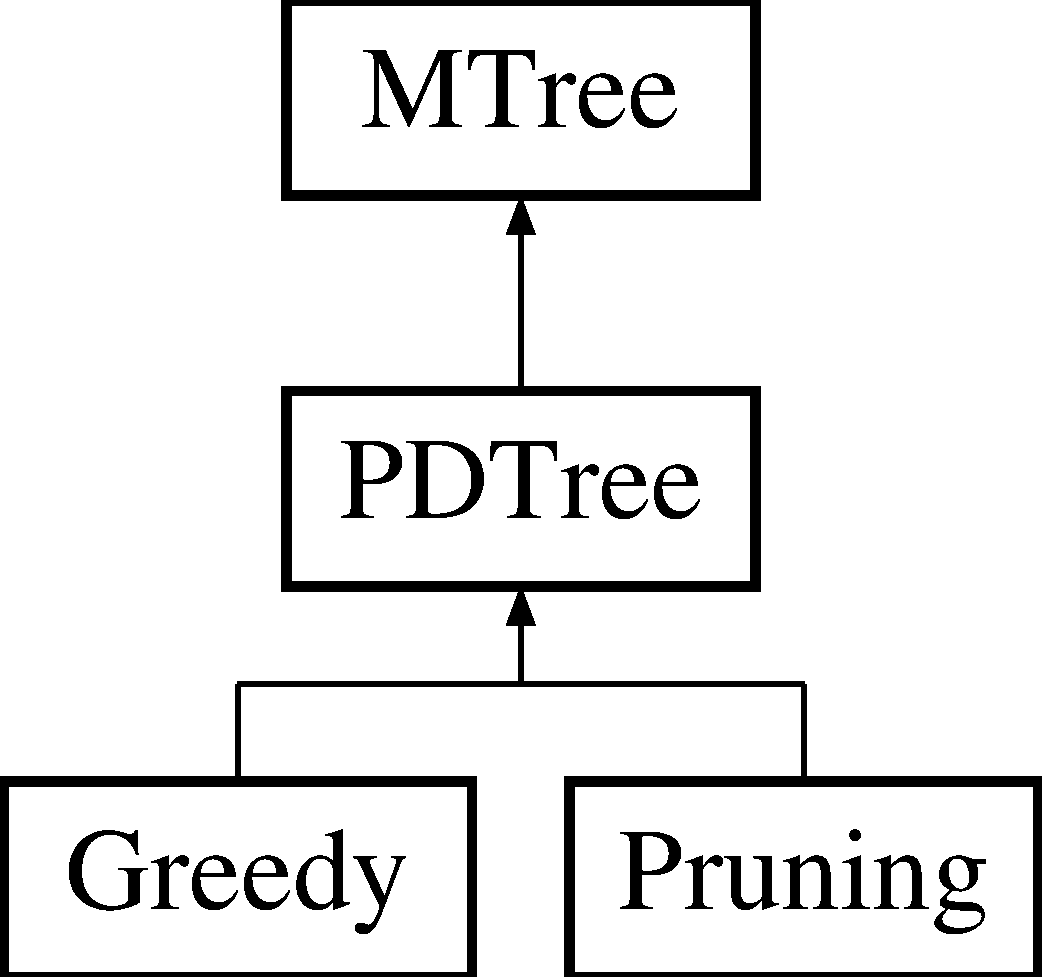
\includegraphics[height=3cm]{classPDTree}
\end{center}
\end{figure}
\subsection*{Public Member Functions}
\begin{DoxyCompactItemize}
\item 
\hyperlink{classPDTree_a3561a63dd0ff1df68e0705bd3a734802}{PDTree} (\hyperlink{structParams}{Params} \&params)
\item 
\hyperlink{classPDTree_aabcb230432131fcf1a626497582136b7}{PDTree} (\hyperlink{classPDTree}{PDTree} \&tree)
\item 
\hyperlink{classPDTree_afbd93cea8f1f5d76f1b5f5130bf0933f}{PDTree} ()
\item 
void \hyperlink{classPDTree_ac90fad3aa9dd0dd64594a15135c8685a}{init} (\hyperlink{structParams}{Params} \&params)
\item 
void \hyperlink{classPDTree_a423ef933e7940c5c745e27898a394bfc}{init} (\hyperlink{classPDTree}{PDTree} \&tree)
\item 
void \hyperlink{classPDTree_a912f332d0f5b13f4bc6820196af53875}{readParams} (\hyperlink{structParams}{Params} \&params)
\item 
void \hyperlink{classPDTree_a5153f2fadfa0f9a60e1289127afa31b3}{readRootNode} (char $\ast$root\_\-name)
\item 
void \hyperlink{classPDTree_a74fae123a26ba1061e5bba39f2b88525}{readInitialSet} (\hyperlink{structParams}{Params} \&params)
\item 
void \hyperlink{classPDTree_a9a4be8dc6c13aa51a188f17d04a8c492}{incoporateParams} (double \&scale, DoubleVector \&tax\_\-weight, \hyperlink{classNode}{Node} $\ast$node=NULL, \hyperlink{classNode}{Node} $\ast$dad=NULL)
\item 
void \hyperlink{classPDTree_ad309e7ef92c45dcad2e84bad0f216cb1}{buildLeafMapName} (LeafMapName \&lsn, \hyperlink{classNode}{Node} $\ast$node=NULL, \hyperlink{classNode}{Node} $\ast$dad=NULL)
\item 
void \hyperlink{classPDTree_af35a390cd0d1e7d9b24447d356f99ed1}{computePD} (\hyperlink{structParams}{Params} \&params, vector$<$ \hyperlink{classPDTaxaSet}{PDTaxaSet} $>$ \&taxa\_\-set, \hyperlink{structPDRelatedMeasures}{PDRelatedMeasures} \&pd\_\-more)
\item 
void \hyperlink{classPDTree_aff9a948210c8eaeab55b820fb908c3c1}{makeTaxaSet} (set$<$ \hyperlink{classNxsString}{NxsString} $>$ \&taxa\_\-name, \hyperlink{classPDTaxaSet}{PDTaxaSet} \&taxa\_\-set, \hyperlink{classNode}{Node} $\ast$node=NULL, \hyperlink{classNode}{Node} $\ast$dad=NULL)
\item 
bool \hyperlink{classPDTree_a0f7b9ac448266270a1e9d3d18218dc2e}{calcPD} (\hyperlink{classSplit}{Split} \&id\_\-set, double curlen=0.0, \hyperlink{classNode}{Node} $\ast$node=NULL, \hyperlink{classNode}{Node} $\ast$dad=NULL)
\item 
void \hyperlink{classPDTree_afe962ef278b4c52c969d073c8909a3e5}{calcExclusivePD} (\hyperlink{classSplit}{Split} \&id\_\-set)
\item 
void \hyperlink{classPDTree_ade969be738be4cf02944a1093bfbb52d}{calcPDEndemism} (vector$<$ \hyperlink{classPDTaxaSet}{PDTaxaSet} $>$ \&area\_\-set, DoubleVector \&pd\_\-endem)
\item 
void \hyperlink{classPDTree_acc3ea0e90a8788dcdea8d268a7139d31}{calcPDComplementarity} (vector$<$ \hyperlink{classPDTaxaSet}{PDTaxaSet} $>$ \&area\_\-set, char $\ast$area\_\-name, DoubleVector \&pd\_\-comp)
\end{DoxyCompactItemize}
\subsection*{Public Attributes}
\begin{DoxyCompactItemize}
\item 
NodeVector \hyperlink{classPDTree_aeb8c8f4c842f30b7a0d70b32546e7af1}{initialset}
\end{DoxyCompactItemize}


\subsection{Detailed Description}
Specialized Tree for Phylogenetic Diversity Algorithms \begin{DoxyAuthor}{Author}
BUI Quang Minh, Steffen Klaere, Arndt von Haeseler 
\end{DoxyAuthor}


\subsection{Constructor \& Destructor Documentation}
\hypertarget{classPDTree_a3561a63dd0ff1df68e0705bd3a734802}{
\index{PDTree@{PDTree}!PDTree@{PDTree}}
\index{PDTree@{PDTree}!PDTree@{PDTree}}
\subsubsection[{PDTree}]{\setlength{\rightskip}{0pt plus 5cm}PDTree::PDTree ({\bf Params} \& {\em params})}}
\label{classPDTree_a3561a63dd0ff1df68e0705bd3a734802}
construct from program parameters 
\begin{DoxyParams}{Parameters}
\item[{\em params}]program parameters \end{DoxyParams}
\hypertarget{classPDTree_aabcb230432131fcf1a626497582136b7}{
\index{PDTree@{PDTree}!PDTree@{PDTree}}
\index{PDTree@{PDTree}!PDTree@{PDTree}}
\subsubsection[{PDTree}]{\setlength{\rightskip}{0pt plus 5cm}PDTree::PDTree ({\bf PDTree} \& {\em tree})}}
\label{classPDTree_aabcb230432131fcf1a626497582136b7}
constructor, get from another tree 
\begin{DoxyParams}{Parameters}
\item[{\em tree}]another \hyperlink{classMTree}{MTree}\end{DoxyParams}
constructor \hypertarget{classPDTree_afbd93cea8f1f5d76f1b5f5130bf0933f}{
\index{PDTree@{PDTree}!PDTree@{PDTree}}
\index{PDTree@{PDTree}!PDTree@{PDTree}}
\subsubsection[{PDTree}]{\setlength{\rightskip}{0pt plus 5cm}PDTree::PDTree ()\hspace{0.3cm}{\ttfamily  \mbox{[}inline\mbox{]}}}}
\label{classPDTree_afbd93cea8f1f5d76f1b5f5130bf0933f}
constructor 

\subsection{Member Function Documentation}
\hypertarget{classPDTree_ad309e7ef92c45dcad2e84bad0f216cb1}{
\index{PDTree@{PDTree}!buildLeafMapName@{buildLeafMapName}}
\index{buildLeafMapName@{buildLeafMapName}!PDTree@{PDTree}}
\subsubsection[{buildLeafMapName}]{\setlength{\rightskip}{0pt plus 5cm}void PDTree::buildLeafMapName (LeafMapName \& {\em lsn}, \/  {\bf Node} $\ast$ {\em node} = {\ttfamily NULL}, \/  {\bf Node} $\ast$ {\em dad} = {\ttfamily NULL})}}
\label{classPDTree_ad309e7ef92c45dcad2e84bad0f216cb1}
build a set of leaf name, return to lsn 
\begin{DoxyParams}{Parameters}
\item[{\em node}]the starting node, NULL to start from the root \item[{\em dad}]dad of the node, used to direct the search \item[{\em lsn}](OUT) leaf set name \end{DoxyParams}
\hypertarget{classPDTree_afe962ef278b4c52c969d073c8909a3e5}{
\index{PDTree@{PDTree}!calcExclusivePD@{calcExclusivePD}}
\index{calcExclusivePD@{calcExclusivePD}!PDTree@{PDTree}}
\subsubsection[{calcExclusivePD}]{\setlength{\rightskip}{0pt plus 5cm}void PDTree::calcExclusivePD ({\bf Split} \& {\em id\_\-set})}}
\label{classPDTree_afe962ef278b4c52c969d073c8909a3e5}
compute the EXCLUSIVE PD score of a given taxa set with name in taxa\_\-name 
\begin{DoxyParams}{Parameters}
\item[{\em id\_\-set}](IN/OUT) corresponding set of taxa IDs \end{DoxyParams}
\hypertarget{classPDTree_a0f7b9ac448266270a1e9d3d18218dc2e}{
\index{PDTree@{PDTree}!calcPD@{calcPD}}
\index{calcPD@{calcPD}!PDTree@{PDTree}}
\subsubsection[{calcPD}]{\setlength{\rightskip}{0pt plus 5cm}bool PDTree::calcPD ({\bf Split} \& {\em id\_\-set}, \/  double {\em curlen} = {\ttfamily 0.0}, \/  {\bf Node} $\ast$ {\em node} = {\ttfamily NULL}, \/  {\bf Node} $\ast$ {\em dad} = {\ttfamily NULL})}}
\label{classPDTree_a0f7b9ac448266270a1e9d3d18218dc2e}
compute the PD score of a given taxa set with name in taxa\_\-name 
\begin{DoxyParams}{Parameters}
\item[{\em id\_\-set}](IN/OUT) corresponding set of taxa \item[{\em node}]the starting node, NULL to start from the root \item[{\em dad}]dad of the node, used to direct the search \item[{\em curlen}]current length so far \end{DoxyParams}
\begin{DoxyReturn}{Returns}
TRUE if the below subtree contains taxon in id\_\-set 
\end{DoxyReturn}
\hypertarget{classPDTree_acc3ea0e90a8788dcdea8d268a7139d31}{
\index{PDTree@{PDTree}!calcPDComplementarity@{calcPDComplementarity}}
\index{calcPDComplementarity@{calcPDComplementarity}!PDTree@{PDTree}}
\subsubsection[{calcPDComplementarity}]{\setlength{\rightskip}{0pt plus 5cm}void PDTree::calcPDComplementarity (vector$<$ {\bf PDTaxaSet} $>$ \& {\em area\_\-set}, \/  char $\ast$ {\em area\_\-name}, \/  DoubleVector \& {\em pd\_\-comp})}}
\label{classPDTree_acc3ea0e90a8788dcdea8d268a7139d31}
compute the area's PD complementarity given a specific area 
\begin{DoxyParams}{Parameters}
\item[{\em area\_\-set}]set of area \item[{\em area\_\-name}]given area names as string separated by commas \item[{\em pd\_\-comp}](OUT) corresponding PD endemism \end{DoxyParams}
\hypertarget{classPDTree_ade969be738be4cf02944a1093bfbb52d}{
\index{PDTree@{PDTree}!calcPDEndemism@{calcPDEndemism}}
\index{calcPDEndemism@{calcPDEndemism}!PDTree@{PDTree}}
\subsubsection[{calcPDEndemism}]{\setlength{\rightskip}{0pt plus 5cm}void PDTree::calcPDEndemism (vector$<$ {\bf PDTaxaSet} $>$ \& {\em area\_\-set}, \/  DoubleVector \& {\em pd\_\-endem})}}
\label{classPDTree_ade969be738be4cf02944a1093bfbb52d}
compute the area's PD ENDEMISM of set of area 
\begin{DoxyParams}{Parameters}
\item[{\em area\_\-set}]set of area \item[{\em pd\_\-endem}](OUT) corresponding PD endemism \end{DoxyParams}
\hypertarget{classPDTree_af35a390cd0d1e7d9b24447d356f99ed1}{
\index{PDTree@{PDTree}!computePD@{computePD}}
\index{computePD@{computePD}!PDTree@{PDTree}}
\subsubsection[{computePD}]{\setlength{\rightskip}{0pt plus 5cm}void PDTree::computePD ({\bf Params} \& {\em params}, \/  vector$<$ {\bf PDTaxaSet} $>$ \& {\em taxa\_\-set}, \/  {\bf PDRelatedMeasures} \& {\em pd\_\-more})}}
\label{classPDTree_af35a390cd0d1e7d9b24447d356f99ed1}
compute the PD score of a given taxa set in filename 
\begin{DoxyParams}{Parameters}
\item[{\em params}]program parameters \item[{\em taxa\_\-set}](OUT) corresponding set of taxa \item[{\em pd\_\-more}](OUT) more computed PD measures will be stored here \end{DoxyParams}
\hypertarget{classPDTree_a9a4be8dc6c13aa51a188f17d04a8c492}{
\index{PDTree@{PDTree}!incoporateParams@{incoporateParams}}
\index{incoporateParams@{incoporateParams}!PDTree@{PDTree}}
\subsubsection[{incoporateParams}]{\setlength{\rightskip}{0pt plus 5cm}void PDTree::incoporateParams (double \& {\em scale}, \/  DoubleVector \& {\em tax\_\-weight}, \/  {\bf Node} $\ast$ {\em node} = {\ttfamily NULL}, \/  {\bf Node} $\ast$ {\em dad} = {\ttfamily NULL})}}
\label{classPDTree_a9a4be8dc6c13aa51a188f17d04a8c492}
incoporate the parameters to the tree 
\begin{DoxyParams}{Parameters}
\item[{\em node}]the starting node, NULL to start from the root \item[{\em dad}]dad of the node, used to direct the search \item[{\em scale}](OUT) branch scaling factor \item[{\em tax\_\-weight}](OUT) taxa weights \end{DoxyParams}
\hypertarget{classPDTree_a423ef933e7940c5c745e27898a394bfc}{
\index{PDTree@{PDTree}!init@{init}}
\index{init@{init}!PDTree@{PDTree}}
\subsubsection[{init}]{\setlength{\rightskip}{0pt plus 5cm}void PDTree::init ({\bf PDTree} \& {\em tree})}}
\label{classPDTree_a423ef933e7940c5c745e27898a394bfc}
initialize tree, get from another tree 
\begin{DoxyParams}{Parameters}
\item[{\em tree}]another \hyperlink{classMTree}{MTree} \end{DoxyParams}


Reimplemented from \hyperlink{classMTree_ad7da0ad44a31e8e98262bd7ad0f494ab}{MTree}.\hypertarget{classPDTree_ac90fad3aa9dd0dd64594a15135c8685a}{
\index{PDTree@{PDTree}!init@{init}}
\index{init@{init}!PDTree@{PDTree}}
\subsubsection[{init}]{\setlength{\rightskip}{0pt plus 5cm}void PDTree::init ({\bf Params} \& {\em params})}}
\label{classPDTree_ac90fad3aa9dd0dd64594a15135c8685a}
initialize the tree from program parameters 
\begin{DoxyParams}{Parameters}
\item[{\em params}]program parameters \end{DoxyParams}
\hypertarget{classPDTree_aff9a948210c8eaeab55b820fb908c3c1}{
\index{PDTree@{PDTree}!makeTaxaSet@{makeTaxaSet}}
\index{makeTaxaSet@{makeTaxaSet}!PDTree@{PDTree}}
\subsubsection[{makeTaxaSet}]{\setlength{\rightskip}{0pt plus 5cm}void PDTree::makeTaxaSet (set$<$ {\bf NxsString} $>$ \& {\em taxa\_\-name}, \/  {\bf PDTaxaSet} \& {\em taxa\_\-set}, \/  {\bf Node} $\ast$ {\em node} = {\ttfamily NULL}, \/  {\bf Node} $\ast$ {\em dad} = {\ttfamily NULL})}}
\label{classPDTree_aff9a948210c8eaeab55b820fb908c3c1}
compute the PD score of a given taxa set with name in taxa\_\-name 
\begin{DoxyParams}{Parameters}
\item[{\em taxa\_\-name}]vector of name of all taxa \item[{\em taxa\_\-set}](OUT) corresponding set of taxa \item[{\em node}]the starting node, NULL to start from the root \item[{\em dad}]dad of the node, used to direct the search \end{DoxyParams}
\hypertarget{classPDTree_a74fae123a26ba1061e5bba39f2b88525}{
\index{PDTree@{PDTree}!readInitialSet@{readInitialSet}}
\index{readInitialSet@{readInitialSet}!PDTree@{PDTree}}
\subsubsection[{readInitialSet}]{\setlength{\rightskip}{0pt plus 5cm}void PDTree::readInitialSet ({\bf Params} \& {\em params})}}
\label{classPDTree_a74fae123a26ba1061e5bba39f2b88525}
read the initial set of taxa to be included into PD-\/tree 
\begin{DoxyParams}{Parameters}
\item[{\em params}]program parameters\end{DoxyParams}
read the initial set of taxa to be included into PD-\/tree \hypertarget{classPDTree_a912f332d0f5b13f4bc6820196af53875}{
\index{PDTree@{PDTree}!readParams@{readParams}}
\index{readParams@{readParams}!PDTree@{PDTree}}
\subsubsection[{readParams}]{\setlength{\rightskip}{0pt plus 5cm}void PDTree::readParams ({\bf Params} \& {\em params})}}
\label{classPDTree_a912f332d0f5b13f4bc6820196af53875}
read the parameter from the file 
\begin{DoxyParams}{Parameters}
\item[{\em params}]program parameters \end{DoxyParams}
\hypertarget{classPDTree_a5153f2fadfa0f9a60e1289127afa31b3}{
\index{PDTree@{PDTree}!readRootNode@{readRootNode}}
\index{readRootNode@{readRootNode}!PDTree@{PDTree}}
\subsubsection[{readRootNode}]{\setlength{\rightskip}{0pt plus 5cm}void PDTree::readRootNode (char $\ast$ {\em root\_\-name})}}
\label{classPDTree_a5153f2fadfa0f9a60e1289127afa31b3}
Identify the root node if specified, include it into the initial set 
\begin{DoxyParams}{Parameters}
\item[{\em root\_\-name}]name of the root node \end{DoxyParams}


\subsection{Member Data Documentation}
\hypertarget{classPDTree_aeb8c8f4c842f30b7a0d70b32546e7af1}{
\index{PDTree@{PDTree}!initialset@{initialset}}
\index{initialset@{initialset}!PDTree@{PDTree}}
\subsubsection[{initialset}]{\setlength{\rightskip}{0pt plus 5cm}NodeVector {\bf PDTree::initialset}}}
\label{classPDTree_aeb8c8f4c842f30b7a0d70b32546e7af1}
initial set of taxa which must be included into the final PD set 

The documentation for this class was generated from the following files:\begin{DoxyCompactItemize}
\item 
src/pdtree.h\item 
src/pdtree.cpp\end{DoxyCompactItemize}

\hypertarget{classPDTreeSet}{
\section{PDTreeSet Class Reference}
\label{classPDTreeSet}\index{PDTreeSet@{PDTreeSet}}
}


{\ttfamily \#include $<$pdtreeset.h$>$}Inheritance diagram for PDTreeSet::\begin{figure}[H]
\begin{center}
\leavevmode
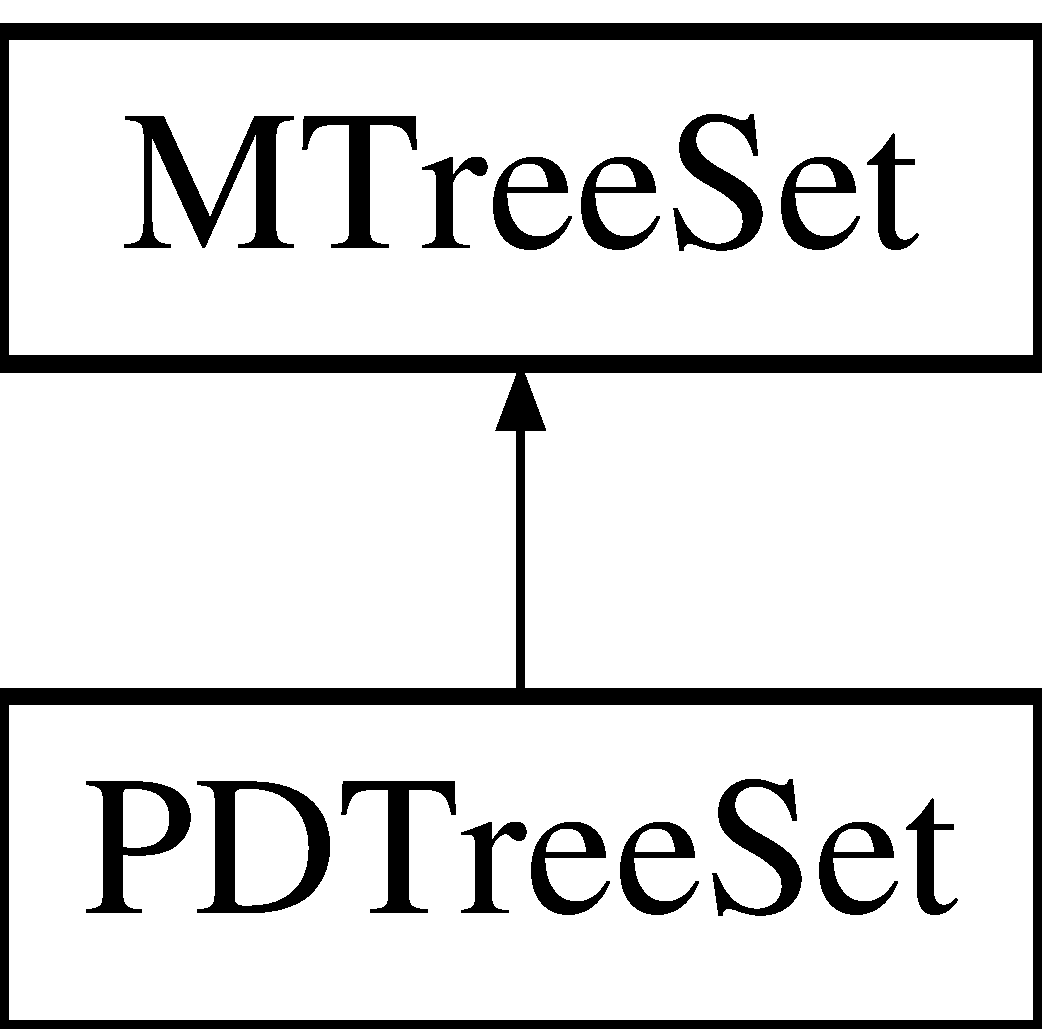
\includegraphics[height=2cm]{classPDTreeSet}
\end{center}
\end{figure}
\subsection*{Public Member Functions}
\begin{DoxyCompactItemize}
\item 
\hyperlink{classPDTreeSet_a168d632f3e858ba8e8c714e8ab85fa45}{PDTreeSet} (\hyperlink{structParams}{Params} \&params)
\item 
virtual \hyperlink{classMTree}{MTree} $\ast$ \hyperlink{classPDTreeSet_a0af6b254e9faff292db3684ec6089e24}{newTree} ()
\item 
bool \hyperlink{classPDTreeSet_ac7e97a1b3130b4b06ce154db0d8f50b9}{isRootedTrees} ()
\item 
int \hyperlink{classPDTreeSet_a9ae4ee3a64ffc0556514a9ea206b9949}{getNTaxa} ()
\item 
void \hyperlink{classPDTreeSet_aabbf34120793461a61cb099aa1095cf2}{init} (\hyperlink{structParams}{Params} \&params)
\item 
void \hyperlink{classPDTreeSet_af2a27a3ed80adb54c44c7cc3f2f43bc1}{readParams} (\hyperlink{structParams}{Params} \&params)
\item 
void \hyperlink{classPDTreeSet_a4ddfd3ac840458f8c73d9b8ff0b03bbc}{readRootNode} (char $\ast$root\_\-name)
\item 
void \hyperlink{classPDTreeSet_a4c5e9cac8a799ad0c2365cfd27dbf153}{readInitialSet} (\hyperlink{structParams}{Params} \&params)
\end{DoxyCompactItemize}
\subsection*{Protected Attributes}
\begin{DoxyCompactItemize}
\item 
StrVector \hyperlink{classPDTreeSet_ae0a51247792a6dc0d1ac141c8beb2ad1}{init\_\-taxa}
\end{DoxyCompactItemize}


\subsection{Detailed Description}
Vector of \hyperlink{classPDTree}{PDTree}

\begin{DoxyAuthor}{Author}
BUI Quang Minh, Steffen Klaere, Arndt von Haeseler 
\end{DoxyAuthor}


\subsection{Constructor \& Destructor Documentation}
\hypertarget{classPDTreeSet_a168d632f3e858ba8e8c714e8ab85fa45}{
\index{PDTreeSet@{PDTreeSet}!PDTreeSet@{PDTreeSet}}
\index{PDTreeSet@{PDTreeSet}!PDTreeSet@{PDTreeSet}}
\subsubsection[{PDTreeSet}]{\setlength{\rightskip}{0pt plus 5cm}PDTreeSet::PDTreeSet ({\bf Params} \& {\em params})}}
\label{classPDTreeSet_a168d632f3e858ba8e8c714e8ab85fa45}
constructor, read trees from user file 
\begin{DoxyParams}{Parameters}
\item[{\em params}]program parameters \end{DoxyParams}


\subsection{Member Function Documentation}
\hypertarget{classPDTreeSet_a9ae4ee3a64ffc0556514a9ea206b9949}{
\index{PDTreeSet@{PDTreeSet}!getNTaxa@{getNTaxa}}
\index{getNTaxa@{getNTaxa}!PDTreeSet@{PDTreeSet}}
\subsubsection[{getNTaxa}]{\setlength{\rightskip}{0pt plus 5cm}int PDTreeSet::getNTaxa ()}}
\label{classPDTreeSet_a9ae4ee3a64ffc0556514a9ea206b9949}
\begin{DoxyReturn}{Returns}
number of taxa 
\end{DoxyReturn}
\hypertarget{classPDTreeSet_aabbf34120793461a61cb099aa1095cf2}{
\index{PDTreeSet@{PDTreeSet}!init@{init}}
\index{init@{init}!PDTreeSet@{PDTreeSet}}
\subsubsection[{init}]{\setlength{\rightskip}{0pt plus 5cm}void PDTreeSet::init ({\bf Params} \& {\em params})}}
\label{classPDTreeSet_aabbf34120793461a61cb099aa1095cf2}
initialize the tree from program parameters 
\begin{DoxyParams}{Parameters}
\item[{\em params}]program parameters \end{DoxyParams}
\hypertarget{classPDTreeSet_ac7e97a1b3130b4b06ce154db0d8f50b9}{
\index{PDTreeSet@{PDTreeSet}!isRootedTrees@{isRootedTrees}}
\index{isRootedTrees@{isRootedTrees}!PDTreeSet@{PDTreeSet}}
\subsubsection[{isRootedTrees}]{\setlength{\rightskip}{0pt plus 5cm}bool PDTreeSet::isRootedTrees ()}}
\label{classPDTreeSet_ac7e97a1b3130b4b06ce154db0d8f50b9}
\begin{DoxyReturn}{Returns}
true if trees are rooted 
\end{DoxyReturn}
\hypertarget{classPDTreeSet_a0af6b254e9faff292db3684ec6089e24}{
\index{PDTreeSet@{PDTreeSet}!newTree@{newTree}}
\index{newTree@{newTree}!PDTreeSet@{PDTreeSet}}
\subsubsection[{newTree}]{\setlength{\rightskip}{0pt plus 5cm}virtual {\bf MTree}$\ast$ PDTreeSet::newTree ()\hspace{0.3cm}{\ttfamily  \mbox{[}inline, virtual\mbox{]}}}}
\label{classPDTreeSet_a0af6b254e9faff292db3684ec6089e24}
\begin{DoxyReturn}{Returns}
a new tree 
\end{DoxyReturn}


Reimplemented from \hyperlink{classMTreeSet_a14f065ce54450ea54f3fd8e1cc025103}{MTreeSet}.\hypertarget{classPDTreeSet_a4c5e9cac8a799ad0c2365cfd27dbf153}{
\index{PDTreeSet@{PDTreeSet}!readInitialSet@{readInitialSet}}
\index{readInitialSet@{readInitialSet}!PDTreeSet@{PDTreeSet}}
\subsubsection[{readInitialSet}]{\setlength{\rightskip}{0pt plus 5cm}void PDTreeSet::readInitialSet ({\bf Params} \& {\em params})}}
\label{classPDTreeSet_a4c5e9cac8a799ad0c2365cfd27dbf153}
read the initial set of taxa to be included into PD-\/tree 
\begin{DoxyParams}{Parameters}
\item[{\em params}]program parameters\end{DoxyParams}
read the initial set of taxa to be included into PD-\/tree \hypertarget{classPDTreeSet_af2a27a3ed80adb54c44c7cc3f2f43bc1}{
\index{PDTreeSet@{PDTreeSet}!readParams@{readParams}}
\index{readParams@{readParams}!PDTreeSet@{PDTreeSet}}
\subsubsection[{readParams}]{\setlength{\rightskip}{0pt plus 5cm}void PDTreeSet::readParams ({\bf Params} \& {\em params})}}
\label{classPDTreeSet_af2a27a3ed80adb54c44c7cc3f2f43bc1}
read the parameter from the file 
\begin{DoxyParams}{Parameters}
\item[{\em params}]program parameters \end{DoxyParams}
\hypertarget{classPDTreeSet_a4ddfd3ac840458f8c73d9b8ff0b03bbc}{
\index{PDTreeSet@{PDTreeSet}!readRootNode@{readRootNode}}
\index{readRootNode@{readRootNode}!PDTreeSet@{PDTreeSet}}
\subsubsection[{readRootNode}]{\setlength{\rightskip}{0pt plus 5cm}void PDTreeSet::readRootNode (char $\ast$ {\em root\_\-name})}}
\label{classPDTreeSet_a4ddfd3ac840458f8c73d9b8ff0b03bbc}
Identify the root node if specified, include it into the initial set 
\begin{DoxyParams}{Parameters}
\item[{\em root\_\-name}]name of the root node \end{DoxyParams}


\subsection{Member Data Documentation}
\hypertarget{classPDTreeSet_ae0a51247792a6dc0d1ac141c8beb2ad1}{
\index{PDTreeSet@{PDTreeSet}!init\_\-taxa@{init\_\-taxa}}
\index{init\_\-taxa@{init\_\-taxa}!PDTreeSet@{PDTreeSet}}
\subsubsection[{init\_\-taxa}]{\setlength{\rightskip}{0pt plus 5cm}StrVector {\bf PDTreeSet::init\_\-taxa}\hspace{0.3cm}{\ttfamily  \mbox{[}protected\mbox{]}}}}
\label{classPDTreeSet_ae0a51247792a6dc0d1ac141c8beb2ad1}
name of initial taxa, to be included into PD set 

The documentation for this class was generated from the following files:\begin{DoxyCompactItemize}
\item 
src/pdtreeset.h\item 
src/pdtreeset.cpp\end{DoxyCompactItemize}

\hypertarget{classPhyloNeighbor}{
\section{PhyloNeighbor Class Reference}
\label{classPhyloNeighbor}\index{PhyloNeighbor@{PhyloNeighbor}}
}


{\ttfamily \#include $<$phylonode.h$>$}Inheritance diagram for PhyloNeighbor::\begin{figure}[H]
\begin{center}
\leavevmode
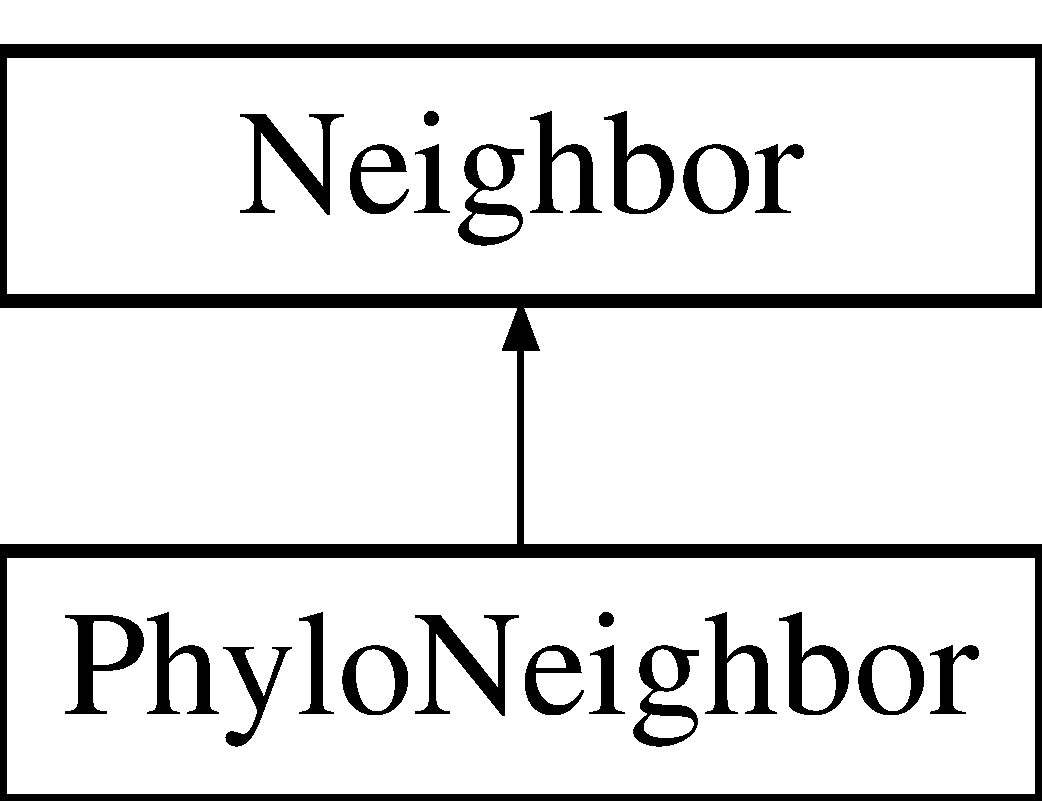
\includegraphics[height=2cm]{classPhyloNeighbor}
\end{center}
\end{figure}
\subsection*{Public Member Functions}
\begin{DoxyCompactItemize}
\item 
\hyperlink{classPhyloNeighbor_a7bed9a973f5f185142219be91e1ca654}{PhyloNeighbor} (\hyperlink{classNode}{Node} $\ast$anode, double alength)
\item 
virtual \hyperlink{classPhyloNeighbor_a60a5db92883b1af1679adab253bf1ce1}{$\sim$PhyloNeighbor} ()
\item 
void \hyperlink{classPhyloNeighbor_a361b1d766721309ab38f6c4ea028adf5}{clearPartialLh} ()
\end{DoxyCompactItemize}
\subsection*{Friends}
\begin{DoxyCompactItemize}
\item 
\hypertarget{classPhyloNeighbor_abd4cfdd3e9b09cc356912ddff682f6c3}{
class \hyperlink{classPhyloNeighbor_abd4cfdd3e9b09cc356912ddff682f6c3}{PhyloNode}}
\label{classPhyloNeighbor_abd4cfdd3e9b09cc356912ddff682f6c3}

\item 
\hypertarget{classPhyloNeighbor_a38fa7a30e653e52f48d662f26bd549be}{
class \hyperlink{classPhyloNeighbor_a38fa7a30e653e52f48d662f26bd549be}{PhyloTree}}
\label{classPhyloNeighbor_a38fa7a30e653e52f48d662f26bd549be}

\end{DoxyCompactItemize}


\subsection{Detailed Description}
A neighbor in a phylogenetic tree

\begin{DoxyAuthor}{Author}
BUI Quang Minh, Steffen Klaere, Arndt von Haeseler $<$\href{mailto:minh.bui@univie.ac.at}{\tt minh.bui@univie.ac.at}$>$ 
\end{DoxyAuthor}


\subsection{Constructor \& Destructor Documentation}
\hypertarget{classPhyloNeighbor_a7bed9a973f5f185142219be91e1ca654}{
\index{PhyloNeighbor@{PhyloNeighbor}!PhyloNeighbor@{PhyloNeighbor}}
\index{PhyloNeighbor@{PhyloNeighbor}!PhyloNeighbor@{PhyloNeighbor}}
\subsubsection[{PhyloNeighbor}]{\setlength{\rightskip}{0pt plus 5cm}PhyloNeighbor::PhyloNeighbor ({\bf Node} $\ast$ {\em anode}, \/  double {\em alength})\hspace{0.3cm}{\ttfamily  \mbox{[}inline\mbox{]}}}}
\label{classPhyloNeighbor_a7bed9a973f5f185142219be91e1ca654}
construct class with a node and length 
\begin{DoxyParams}{Parameters}
\item[{\em anode}]the other end of the branch \item[{\em alength}]length of branch \end{DoxyParams}
\hypertarget{classPhyloNeighbor_a60a5db92883b1af1679adab253bf1ce1}{
\index{PhyloNeighbor@{PhyloNeighbor}!$\sim$PhyloNeighbor@{$\sim$PhyloNeighbor}}
\index{$\sim$PhyloNeighbor@{$\sim$PhyloNeighbor}!PhyloNeighbor@{PhyloNeighbor}}
\subsubsection[{$\sim$PhyloNeighbor}]{\setlength{\rightskip}{0pt plus 5cm}virtual PhyloNeighbor::$\sim$PhyloNeighbor ()\hspace{0.3cm}{\ttfamily  \mbox{[}inline, virtual\mbox{]}}}}
\label{classPhyloNeighbor_a60a5db92883b1af1679adab253bf1ce1}
destructor 

\subsection{Member Function Documentation}
\hypertarget{classPhyloNeighbor_a361b1d766721309ab38f6c4ea028adf5}{
\index{PhyloNeighbor@{PhyloNeighbor}!clearPartialLh@{clearPartialLh}}
\index{clearPartialLh@{clearPartialLh}!PhyloNeighbor@{PhyloNeighbor}}
\subsubsection[{clearPartialLh}]{\setlength{\rightskip}{0pt plus 5cm}void PhyloNeighbor::clearPartialLh ()\hspace{0.3cm}{\ttfamily  \mbox{[}inline\mbox{]}}}}
\label{classPhyloNeighbor_a361b1d766721309ab38f6c4ea028adf5}
tell that the partial likelihood vector is not computed 

The documentation for this class was generated from the following file:\begin{DoxyCompactItemize}
\item 
src/phylonode.h\end{DoxyCompactItemize}

\hypertarget{classPhyloNode}{
\section{PhyloNode Class Reference}
\label{classPhyloNode}\index{PhyloNode@{PhyloNode}}
}


{\ttfamily \#include $<$phylonode.h$>$}Inheritance diagram for PhyloNode::\begin{figure}[H]
\begin{center}
\leavevmode
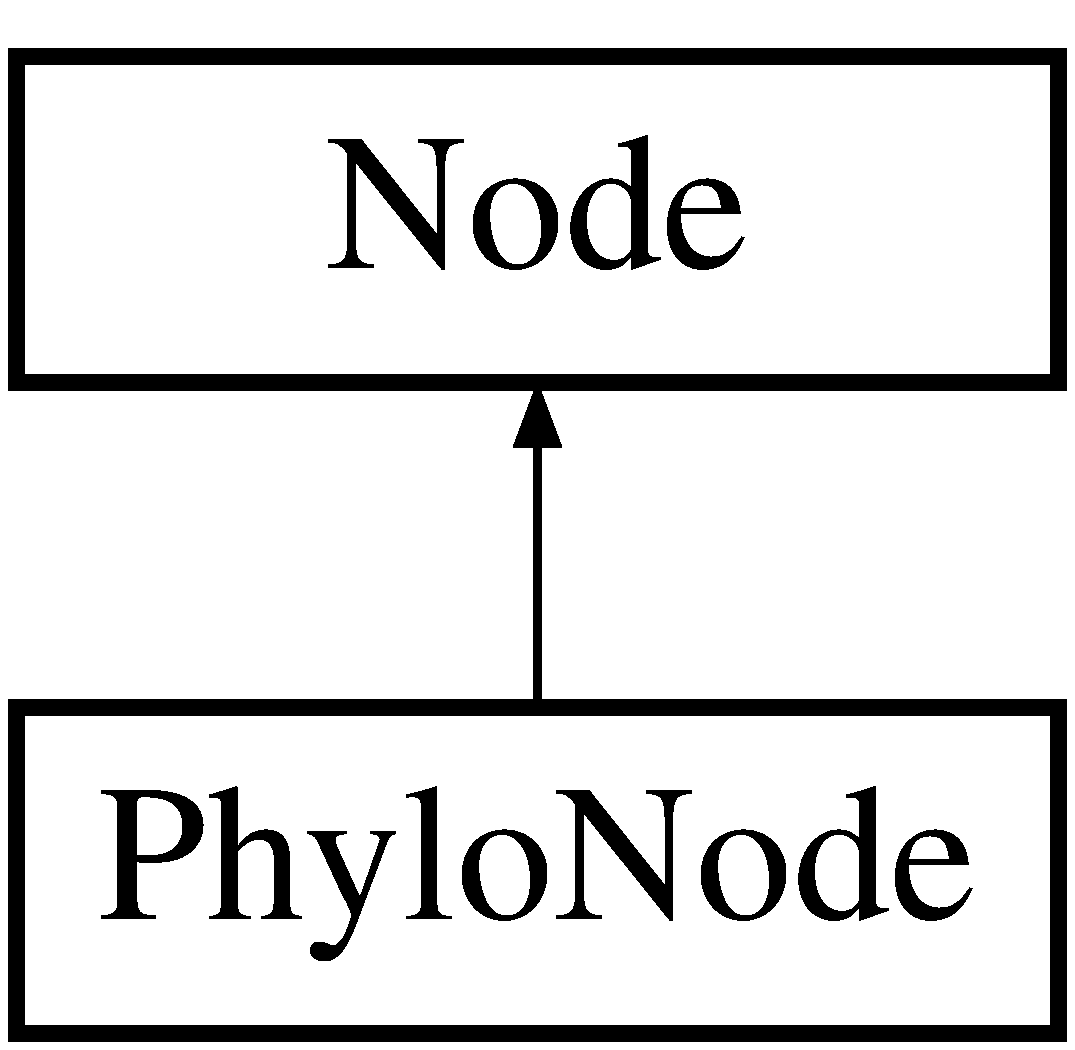
\includegraphics[height=2cm]{classPhyloNode}
\end{center}
\end{figure}
\subsection*{Public Member Functions}
\begin{DoxyCompactItemize}
\item 
\hyperlink{classPhyloNode_a82abba4349a6808ba134a89fae92fb7f}{PhyloNode} ()
\item 
\hyperlink{classPhyloNode_a07225896ff0a5e57a286f6deedef2421}{PhyloNode} (int aid)
\item 
\hyperlink{classPhyloNode_ae89376e4022663801fb2d83e2d55afbe}{PhyloNode} (int aid, int aname)
\item 
\hyperlink{classPhyloNode_aa0ef98742403e238c9ee2789cc9d4a51}{PhyloNode} (int aid, const char $\ast$aname)
\item 
void \hyperlink{classPhyloNode_abb09e14a95714aa6d590c893700be656}{init} ()
\item 
virtual void \hyperlink{classPhyloNode_a626f3e6259921ebf7769dcb19858c825}{addNeighbor} (\hyperlink{classNode}{Node} $\ast$node, double length)
\item 
void \hyperlink{classPhyloNode_a70a516028a492af1eb1a5108d04cbc5f}{clearAllPartialLh} (\hyperlink{classPhyloNode}{PhyloNode} $\ast$dad)
\item 
void \hyperlink{classPhyloNode_ad752a7a4155b10d7b46d1f92afa9acc5}{clearReversePartialLh} (\hyperlink{classPhyloNode}{PhyloNode} $\ast$dad)
\end{DoxyCompactItemize}
\subsection*{Friends}
\begin{DoxyCompactItemize}
\item 
\hypertarget{classPhyloNode_a38fa7a30e653e52f48d662f26bd549be}{
class \hyperlink{classPhyloNode_a38fa7a30e653e52f48d662f26bd549be}{PhyloTree}}
\label{classPhyloNode_a38fa7a30e653e52f48d662f26bd549be}

\end{DoxyCompactItemize}


\subsection{Detailed Description}
A node in a phylogenetic tree

\begin{DoxyAuthor}{Author}
BUI Quang Minh, Steffen Klaere, Arndt von Haeseler $<$\href{mailto:minh.bui@univie.ac.at}{\tt minh.bui@univie.ac.at}$>$ 
\end{DoxyAuthor}


\subsection{Constructor \& Destructor Documentation}
\hypertarget{classPhyloNode_a82abba4349a6808ba134a89fae92fb7f}{
\index{PhyloNode@{PhyloNode}!PhyloNode@{PhyloNode}}
\index{PhyloNode@{PhyloNode}!PhyloNode@{PhyloNode}}
\subsubsection[{PhyloNode}]{\setlength{\rightskip}{0pt plus 5cm}PhyloNode::PhyloNode ()}}
\label{classPhyloNode_a82abba4349a6808ba134a89fae92fb7f}
constructor \hypertarget{classPhyloNode_a07225896ff0a5e57a286f6deedef2421}{
\index{PhyloNode@{PhyloNode}!PhyloNode@{PhyloNode}}
\index{PhyloNode@{PhyloNode}!PhyloNode@{PhyloNode}}
\subsubsection[{PhyloNode}]{\setlength{\rightskip}{0pt plus 5cm}PhyloNode::PhyloNode (int {\em aid})}}
\label{classPhyloNode_a07225896ff0a5e57a286f6deedef2421}
constructor 
\begin{DoxyParams}{Parameters}
\item[{\em aid}]id of this node \end{DoxyParams}
\hypertarget{classPhyloNode_ae89376e4022663801fb2d83e2d55afbe}{
\index{PhyloNode@{PhyloNode}!PhyloNode@{PhyloNode}}
\index{PhyloNode@{PhyloNode}!PhyloNode@{PhyloNode}}
\subsubsection[{PhyloNode}]{\setlength{\rightskip}{0pt plus 5cm}PhyloNode::PhyloNode (int {\em aid}, \/  int {\em aname})}}
\label{classPhyloNode_ae89376e4022663801fb2d83e2d55afbe}
constructor 
\begin{DoxyParams}{Parameters}
\item[{\em aid}]id of this node \item[{\em aname}]name of this node \end{DoxyParams}
\hypertarget{classPhyloNode_aa0ef98742403e238c9ee2789cc9d4a51}{
\index{PhyloNode@{PhyloNode}!PhyloNode@{PhyloNode}}
\index{PhyloNode@{PhyloNode}!PhyloNode@{PhyloNode}}
\subsubsection[{PhyloNode}]{\setlength{\rightskip}{0pt plus 5cm}PhyloNode::PhyloNode (int {\em aid}, \/  const char $\ast$ {\em aname})}}
\label{classPhyloNode_aa0ef98742403e238c9ee2789cc9d4a51}
constructor 
\begin{DoxyParams}{Parameters}
\item[{\em aid}]id of this node \item[{\em aname}]name of this node \end{DoxyParams}


\subsection{Member Function Documentation}
\hypertarget{classPhyloNode_a626f3e6259921ebf7769dcb19858c825}{
\index{PhyloNode@{PhyloNode}!addNeighbor@{addNeighbor}}
\index{addNeighbor@{addNeighbor}!PhyloNode@{PhyloNode}}
\subsubsection[{addNeighbor}]{\setlength{\rightskip}{0pt plus 5cm}void PhyloNode::addNeighbor ({\bf Node} $\ast$ {\em node}, \/  double {\em length})\hspace{0.3cm}{\ttfamily  \mbox{[}virtual\mbox{]}}}}
\label{classPhyloNode_a626f3e6259921ebf7769dcb19858c825}
add a neighbor 
\begin{DoxyParams}{Parameters}
\item[{\em node}]the neighbor node \item[{\em length}]branch length \end{DoxyParams}
\hypertarget{classPhyloNode_a70a516028a492af1eb1a5108d04cbc5f}{
\index{PhyloNode@{PhyloNode}!clearAllPartialLh@{clearAllPartialLh}}
\index{clearAllPartialLh@{clearAllPartialLh}!PhyloNode@{PhyloNode}}
\subsubsection[{clearAllPartialLh}]{\setlength{\rightskip}{0pt plus 5cm}void PhyloNode::clearAllPartialLh ({\bf PhyloNode} $\ast$ {\em dad})}}
\label{classPhyloNode_a70a516028a492af1eb1a5108d04cbc5f}
tell that all partial likelihood vectors below this node are not computed \hypertarget{classPhyloNode_ad752a7a4155b10d7b46d1f92afa9acc5}{
\index{PhyloNode@{PhyloNode}!clearReversePartialLh@{clearReversePartialLh}}
\index{clearReversePartialLh@{clearReversePartialLh}!PhyloNode@{PhyloNode}}
\subsubsection[{clearReversePartialLh}]{\setlength{\rightskip}{0pt plus 5cm}void PhyloNode::clearReversePartialLh ({\bf PhyloNode} $\ast$ {\em dad})}}
\label{classPhyloNode_ad752a7a4155b10d7b46d1f92afa9acc5}
tell that all partial likelihood vectors (in reverse direction) below this node are not computed \hypertarget{classPhyloNode_abb09e14a95714aa6d590c893700be656}{
\index{PhyloNode@{PhyloNode}!init@{init}}
\index{init@{init}!PhyloNode@{PhyloNode}}
\subsubsection[{init}]{\setlength{\rightskip}{0pt plus 5cm}void PhyloNode::init ()}}
\label{classPhyloNode_abb09e14a95714aa6d590c893700be656}
initialization 

The documentation for this class was generated from the following files:\begin{DoxyCompactItemize}
\item 
src/phylonode.h\item 
src/phylonode.cpp\end{DoxyCompactItemize}

\hypertarget{classPhyloTree}{
\section{PhyloTree Class Reference}
\label{classPhyloTree}\index{PhyloTree@{PhyloTree}}
}


{\ttfamily \#include $<$phylotree.h$>$}Inheritance diagram for PhyloTree::\begin{figure}[H]
\begin{center}
\leavevmode
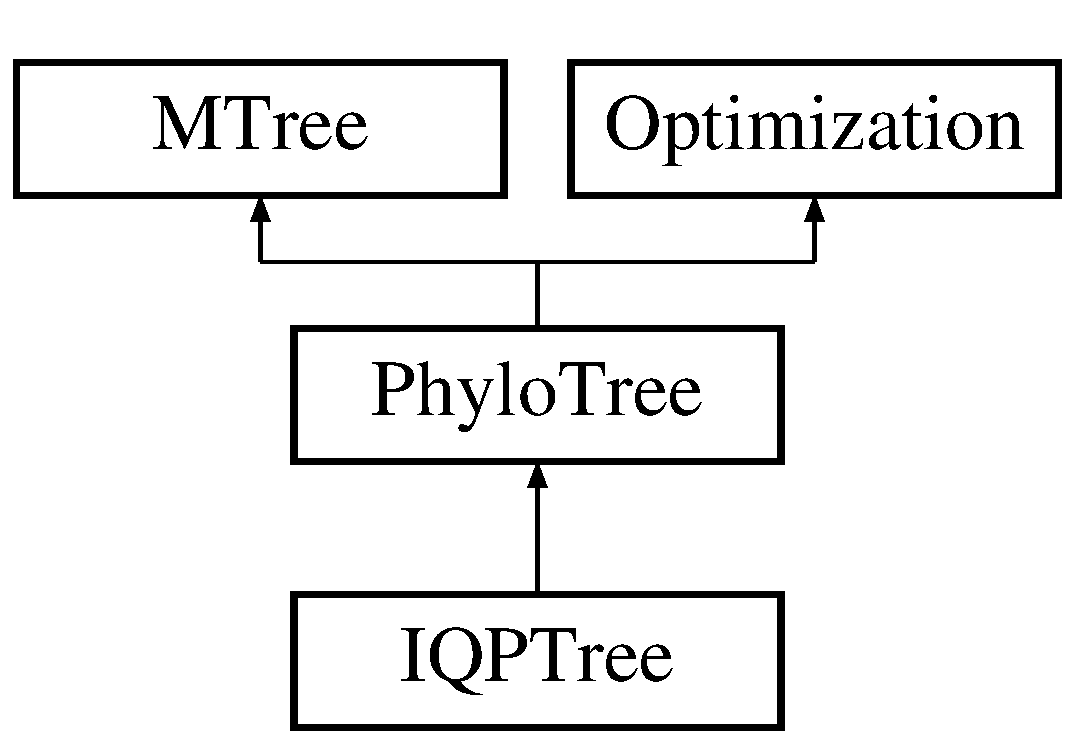
\includegraphics[height=3cm]{classPhyloTree}
\end{center}
\end{figure}
\subsection*{Public Member Functions}
\begin{DoxyCompactItemize}
\item 
\hyperlink{classPhyloTree_ab6e00efe0c10f4a93d34e7d027489ac6}{PhyloTree} ()
\item 
virtual void \hyperlink{classPhyloTree_adce7d871ad6fb36424fab1aa2b688f9a}{copyTree} (\hyperlink{classMTree}{MTree} $\ast$tree)
\item 
void \hyperlink{classPhyloTree_a195bfdd19700eb12a6680ced3bc5193b}{copyPhyloTree} (\hyperlink{classPhyloTree}{PhyloTree} $\ast$tree)
\item 
void \hyperlink{classPhyloTree_a6ea47346f05772215efc900309120428}{setAlignment} (\hyperlink{classAlignment}{Alignment} $\ast$alignment)
\item 
void \hyperlink{classPhyloTree_a0e90911542265b82a3ed52da08bf9187}{setModel} (\hyperlink{classSubstModel}{SubstModel} $\ast$amodel)
\item 
void \hyperlink{classPhyloTree_ad25ae1a621d627f255d9cd8563675165}{setRate} (\hyperlink{classRateHeterogeneity}{RateHeterogeneity} $\ast$rate)
\item 
void \hyperlink{classPhyloTree_afd022a3beda4f24e47b71046d56d4fbf}{createModel} (\hyperlink{structParams}{Params} \&params)
\item 
virtual \hyperlink{classNode}{Node} $\ast$ \hyperlink{classPhyloTree_a08daeabbb3fa596916aa48834e0b152d}{newNode} (int node\_\-id=-\/1, const char $\ast$node\_\-name=NULL)
\item 
virtual \hyperlink{classNode}{Node} $\ast$ \hyperlink{classPhyloTree_a10e2a1d34d9f9751c42c262e1ef7581e}{newNode} (int node\_\-id, int node\_\-name)
\item 
void \hyperlink{classPhyloTree_a1dc84a489c3471eff561658ab98a286a}{clearAllPartialLh} ()
\item 
int \hyperlink{classPhyloTree_a106e4c54e0e3e8d48d3922d205941e60}{computeParsimonyScore} ()
\item 
int \hyperlink{classPhyloTree_a43540029a0627fb2736464a7def1f846}{computeParsimonyScore} (int ptn, int \&states, \hyperlink{classPhyloNode}{PhyloNode} $\ast$node=NULL, \hyperlink{classPhyloNode}{PhyloNode} $\ast$dad=NULL)
\item 
double $\ast$ \hyperlink{classPhyloTree_a3a0f7bf2fc3b545f1ccb6ad2dc8d887c}{newPartialLh} ()
\item 
void \hyperlink{classPhyloTree_a1c65fd0bcc5b433e6dd4781432aaaccd}{computePartialLikelihood} (\hyperlink{classPhyloNeighbor}{PhyloNeighbor} $\ast$dad\_\-branch, \hyperlink{classPhyloNode}{PhyloNode} $\ast$dad=NULL)
\item 
double \hyperlink{classPhyloTree_a375b6b1fe6d56698b804af890a629869}{computeLikelihoodBranch} (\hyperlink{classPhyloNeighbor}{PhyloNeighbor} $\ast$dad\_\-branch, \hyperlink{classPhyloNode}{PhyloNode} $\ast$dad)
\item 
double \hyperlink{classPhyloTree_a7d6a388ffa393ccf810e8e04718725ec}{computeLikelihood} ()
\item 
virtual double \hyperlink{classPhyloTree_a1e1bf7936bb8a7dbacd92f93dad6d531}{optimizeModel} ()
\item 
double \hyperlink{classPhyloTree_a1c21d2ba4fc8755b3435b5677938a0fb}{computeLikelihoodDerv} (\hyperlink{classPhyloNeighbor}{PhyloNeighbor} $\ast$dad\_\-branch, \hyperlink{classPhyloNode}{PhyloNode} $\ast$dad, double \&df, double \&ddf)
\item 
void \hyperlink{classPhyloTree_a9537038984ab81f946a6025d5607637e}{searchNNI} ()
\item 
double \hyperlink{classPhyloTree_a87ed271cb0d09ad3069a20d996c343f9}{searchNNI} (double cur\_\-score, \hyperlink{classPhyloNode}{PhyloNode} $\ast$node=NULL, \hyperlink{classPhyloNode}{PhyloNode} $\ast$dad=NULL)
\item 
double \hyperlink{classPhyloTree_ad5019f595c9fe481d3eb326bcf10fb03}{swapNNI} (double cur\_\-score, \hyperlink{classPhyloNode}{PhyloNode} $\ast$node1, \hyperlink{classPhyloNode}{PhyloNode} $\ast$node2)
\item 
double \hyperlink{classPhyloTree_a93e28f41404baeca2afcb62f4499a3e1}{optimizeOneBranch} (\hyperlink{classPhyloNode}{PhyloNode} $\ast$node1, \hyperlink{classPhyloNode}{PhyloNode} $\ast$node2)
\item 
double \hyperlink{classPhyloTree_aaad81a0e6fc24cfb5b665655059bc17b}{optimizeChildBranches} (\hyperlink{classPhyloNode}{PhyloNode} $\ast$node, \hyperlink{classPhyloNode}{PhyloNode} $\ast$dad=NULL)
\item 
double \hyperlink{classPhyloTree_ab256efc9eb59170ba486c9b6d6d684c7}{optimizeAllBranches} (\hyperlink{classPhyloNode}{PhyloNode} $\ast$node, \hyperlink{classPhyloNode}{PhyloNode} $\ast$dad=NULL)
\item 
double \hyperlink{classPhyloTree_a0d95172300892b57830027c134d7e181}{optimizeAllBranches} (int iterations=100)
\item 
virtual double \hyperlink{classPhyloTree_a34c7bdc00d48d66e1a8ebfee9af1f100}{computeFunction} (double value)
\item 
virtual double \hyperlink{classPhyloTree_a9ae5f61aa0d22976b2d2e8f3ed15f44f}{computeFuncDerv} (double value, double \&df, double \&ddf)
\item 
double \hyperlink{classPhyloTree_acef313906a2021de5de2eb87226a202d}{optimizeNNIBranches} ()
\item 
virtual double \hyperlink{classPhyloTree_a8927dbf75a06ea797cc76b619759985d}{optimizeNNI} ()
\item 
double \hyperlink{classPhyloTree_abd42e1cc3b3da9e0d00ea00182a031d2}{optimizeNNI} (double cur\_\-score, \hyperlink{classPhyloNode}{PhyloNode} $\ast$node=NULL, \hyperlink{classPhyloNode}{PhyloNode} $\ast$dad=NULL)
\item 
double \hyperlink{classPhyloTree_ab846b2730dd57366d4d5c8412870cd9a}{swapNNIBranch} (double cur\_\-score, \hyperlink{classPhyloNode}{PhyloNode} $\ast$node1, \hyperlink{classPhyloNode}{PhyloNode} $\ast$node2)
\item 
void \hyperlink{classPhyloTree_a2de074f797940b19f9b1e923fe6c814a}{growTreeML} (\hyperlink{classAlignment}{Alignment} $\ast$alignment)
\item 
double \hyperlink{classPhyloTree_aa5fdafe246a24235967981a2df3faffb}{addTaxonML} (\hyperlink{classNode}{Node} $\ast$added\_\-node, \hyperlink{classNode}{Node} $\ast$\&target\_\-node, \hyperlink{classNode}{Node} $\ast$\&target\_\-dad, \hyperlink{classNode}{Node} $\ast$node, \hyperlink{classNode}{Node} $\ast$dad)
\item 
void \hyperlink{classPhyloTree_a760299b108adf89646a22ab1ad195cda}{computeBioNJ} (\hyperlink{structParams}{Params} \&params, \hyperlink{classAlignment}{Alignment} $\ast$alignment, double $\ast$\&dist\_\-mat)
\item 
void \hyperlink{classPhyloTree_a80df879587ccb9aa1b9b54103e87ab8a}{fixNegativeBranch} (\hyperlink{classNode}{Node} $\ast$node=NULL, \hyperlink{classNode}{Node} $\ast$dad=NULL)
\item 
double \hyperlink{classPhyloTree_ae2a229415387b5eb9f36c3bb078b6d80}{optimizeSPR} ()
\item 
double \hyperlink{classPhyloTree_a071475b37be90fb615e26b38d72a574f}{optimizeSPRBranches} ()
\item 
double \hyperlink{classPhyloTree_a726b99499f5a40395fc3c825d2d0a9ad}{optimizeSPR} (double cur\_\-score, \hyperlink{classPhyloNode}{PhyloNode} $\ast$node=NULL, \hyperlink{classPhyloNode}{PhyloNode} $\ast$dad=NULL)
\item 
double \hyperlink{classPhyloTree_a50a289b7af25842a1401856fee67d725}{swapSPR} (double cur\_\-score, int cur\_\-depth, \hyperlink{classPhyloNode}{PhyloNode} $\ast$node1, \hyperlink{classPhyloNode}{PhyloNode} $\ast$dad1, \hyperlink{classPhyloNode}{PhyloNode} $\ast$orig\_\-node1, \hyperlink{classPhyloNode}{PhyloNode} $\ast$orig\_\-node2, \hyperlink{classPhyloNode}{PhyloNode} $\ast$node2, \hyperlink{classPhyloNode}{PhyloNode} $\ast$dad2, vector$<$ \hyperlink{classPhyloNeighbor}{PhyloNeighbor} $\ast$ $>$ \&spr\_\-path)
\item 
\hypertarget{classPhyloTree_a73cd13227a66c17b96465fdc908e069f}{
double {\bfseries assessSPRMove} (double cur\_\-score, const \hyperlink{structSPRMove}{SPRMove} \&spr)}
\label{classPhyloTree_a73cd13227a66c17b96465fdc908e069f}

\item 
\hypertarget{classPhyloTree_a2a4ae0ce3b7ac61a7a870280afb85206}{
void {\bfseries pruneSubtree} (\hyperlink{classPhyloNode}{PhyloNode} $\ast$node, \hyperlink{classPhyloNode}{PhyloNode} $\ast$dad, \hyperlink{structPruningInfo}{PruningInfo} \&info)}
\label{classPhyloTree_a2a4ae0ce3b7ac61a7a870280afb85206}

\item 
\hypertarget{classPhyloTree_aa87d04899ec1ece927f02dbfa989afbf}{
void {\bfseries regraftSubtree} (\hyperlink{structPruningInfo}{PruningInfo} \&info, \hyperlink{classPhyloNode}{PhyloNode} $\ast$in\_\-node, \hyperlink{classPhyloNode}{PhyloNode} $\ast$in\_\-dad)}
\label{classPhyloTree_aa87d04899ec1ece927f02dbfa989afbf}

\end{DoxyCompactItemize}
\subsection*{Public Attributes}
\begin{DoxyCompactItemize}
\item 
\hyperlink{classAlignment}{Alignment} $\ast$ \hyperlink{classPhyloTree_a155032795a2a06262959ecba6fa1761b}{aln}
\item 
bool \hyperlink{classPhyloTree_ab17482e0cf6b9ea6def40d2c49bf0f3a}{optimize\_\-by\_\-newton}
\end{DoxyCompactItemize}
\subsection*{Protected Member Functions}
\begin{DoxyCompactItemize}
\item 
void \hyperlink{classPhyloTree_a5a35504080c18e60b3a3019c8d457253}{assignLeafNames} (\hyperlink{classNode}{Node} $\ast$node=NULL, \hyperlink{classNode}{Node} $\ast$dad=NULL)
\end{DoxyCompactItemize}
\subsection*{Protected Attributes}
\begin{DoxyCompactItemize}
\item 
\hyperlink{classSubstModel}{SubstModel} $\ast$ \hyperlink{classPhyloTree_affd265bc9cd055d0f59bfda46c98387b}{model}
\item 
\hyperlink{classRateHeterogeneity}{RateHeterogeneity} $\ast$ \hyperlink{classPhyloTree_a9b7513b9bfee50bcd6cbe97a87366c4d}{site\_\-rate}
\item 
\hyperlink{classPhyloNeighbor}{PhyloNeighbor} $\ast$ \hyperlink{classPhyloTree_a9a11206ad156f382ee0db5f92dd399ce}{current\_\-it}
\item 
\hyperlink{classPhyloNeighbor}{PhyloNeighbor} $\ast$ \hyperlink{classPhyloTree_a5016a4372500fe919bfa09b713cd2344}{current\_\-it\_\-back}
\item 
\hyperlink{classSPRMoves}{SPRMoves} \hyperlink{classPhyloTree_a0ec867545e10bf1a45c938ed5c4a43f1}{spr\_\-moves}
\item 
int \hyperlink{classPhyloTree_a63a5b49b525b22534b525d7a35e663c7}{spr\_\-radius}
\end{DoxyCompactItemize}


\subsection{Detailed Description}
Phylogenetic Tree class

\begin{DoxyAuthor}{Author}
BUI Quang Minh, Steffen Klaere, Arndt von Haeseler $<$\href{mailto:minh.bui@univie.ac.at}{\tt minh.bui@univie.ac.at}$>$ 
\end{DoxyAuthor}


\subsection{Constructor \& Destructor Documentation}
\hypertarget{classPhyloTree_ab6e00efe0c10f4a93d34e7d027489ac6}{
\index{PhyloTree@{PhyloTree}!PhyloTree@{PhyloTree}}
\index{PhyloTree@{PhyloTree}!PhyloTree@{PhyloTree}}
\subsubsection[{PhyloTree}]{\setlength{\rightskip}{0pt plus 5cm}PhyloTree::PhyloTree ()}}
\label{classPhyloTree_ab6e00efe0c10f4a93d34e7d027489ac6}
constructor 

\subsection{Member Function Documentation}
\hypertarget{classPhyloTree_aa5fdafe246a24235967981a2df3faffb}{
\index{PhyloTree@{PhyloTree}!addTaxonML@{addTaxonML}}
\index{addTaxonML@{addTaxonML}!PhyloTree@{PhyloTree}}
\subsubsection[{addTaxonML}]{\setlength{\rightskip}{0pt plus 5cm}double PhyloTree::addTaxonML ({\bf Node} $\ast$ {\em added\_\-node}, \/  {\bf Node} $\ast$\& {\em target\_\-node}, \/  {\bf Node} $\ast$\& {\em target\_\-dad}, \/  {\bf Node} $\ast$ {\em node}, \/  {\bf Node} $\ast$ {\em dad})}}
\label{classPhyloTree_aa5fdafe246a24235967981a2df3faffb}
used internally by \hyperlink{classPhyloTree_a2de074f797940b19f9b1e923fe6c814a}{growTreeML()} to find the best target branch to add into the tree 
\begin{DoxyParams}{Parameters}
\item[{\em added\_\-node}]node to add \item[{\em target\_\-node}](OUT) one end of the best branch found \item[{\em target\_\-dad}](OUT) the other end of the best branch found \item[{\em node}]the current node \item[{\em dad}]dad of the node, used to direct the search \end{DoxyParams}
\begin{DoxyReturn}{Returns}
the likelihood of the tree 
\end{DoxyReturn}
\hypertarget{classPhyloTree_a5a35504080c18e60b3a3019c8d457253}{
\index{PhyloTree@{PhyloTree}!assignLeafNames@{assignLeafNames}}
\index{assignLeafNames@{assignLeafNames}!PhyloTree@{PhyloTree}}
\subsubsection[{assignLeafNames}]{\setlength{\rightskip}{0pt plus 5cm}void PhyloTree::assignLeafNames ({\bf Node} $\ast$ {\em node} = {\ttfamily NULL}, \/  {\bf Node} $\ast$ {\em dad} = {\ttfamily NULL})\hspace{0.3cm}{\ttfamily  \mbox{[}protected\mbox{]}}}}
\label{classPhyloTree_a5a35504080c18e60b3a3019c8d457253}
assign the leaf names with the alignment sequence names, using the leaf ID for assignment. 
\begin{DoxyParams}{Parameters}
\item[{\em node}]the starting node, NULL to start from the root \item[{\em dad}]dad of the node, used to direct the search \end{DoxyParams}
\hypertarget{classPhyloTree_a1dc84a489c3471eff561658ab98a286a}{
\index{PhyloTree@{PhyloTree}!clearAllPartialLh@{clearAllPartialLh}}
\index{clearAllPartialLh@{clearAllPartialLh}!PhyloTree@{PhyloTree}}
\subsubsection[{clearAllPartialLh}]{\setlength{\rightskip}{0pt plus 5cm}void PhyloTree::clearAllPartialLh ()}}
\label{classPhyloTree_a1dc84a489c3471eff561658ab98a286a}
clear all partial likelihood for a clean computation again \hypertarget{classPhyloTree_a760299b108adf89646a22ab1ad195cda}{
\index{PhyloTree@{PhyloTree}!computeBioNJ@{computeBioNJ}}
\index{computeBioNJ@{computeBioNJ}!PhyloTree@{PhyloTree}}
\subsubsection[{computeBioNJ}]{\setlength{\rightskip}{0pt plus 5cm}void PhyloTree::computeBioNJ ({\bf Params} \& {\em params}, \/  {\bf Alignment} $\ast$ {\em alignment}, \/  double $\ast$\& {\em dist\_\-mat})}}
\label{classPhyloTree_a760299b108adf89646a22ab1ad195cda}
compute BioNJ tree 
\begin{DoxyParams}{Parameters}
\item[{\em params}]program parameters \item[{\em alignment}]input alignment \item[{\em dist\_\-mat}](OUT) distance matrix \end{DoxyParams}
\hypertarget{classPhyloTree_a9ae5f61aa0d22976b2d2e8f3ed15f44f}{
\index{PhyloTree@{PhyloTree}!computeFuncDerv@{computeFuncDerv}}
\index{computeFuncDerv@{computeFuncDerv}!PhyloTree@{PhyloTree}}
\subsubsection[{computeFuncDerv}]{\setlength{\rightskip}{0pt plus 5cm}double PhyloTree::computeFuncDerv (double {\em value}, \/  double \& {\em df}, \/  double \& {\em ddf})\hspace{0.3cm}{\ttfamily  \mbox{[}virtual\mbox{]}}}}
\label{classPhyloTree_a9ae5f61aa0d22976b2d2e8f3ed15f44f}
Inherited from \hyperlink{classOptimization}{Optimization} class. This function calculate f(value), first derivative f'(value) and 2nd derivative f''(value). used by Newton raphson method to minimize the function. 
\begin{DoxyParams}{Parameters}
\item[{\em value}]current branch length \item[{\em df}](OUT) first derivative \item[{\em ddf}](OUT) second derivative \end{DoxyParams}
\begin{DoxyReturn}{Returns}
negative of likelihood (for minimization) 
\end{DoxyReturn}


Reimplemented from \hyperlink{classOptimization_a18bedacde6fd259ff5923c9e936464bd}{Optimization}.\hypertarget{classPhyloTree_a34c7bdc00d48d66e1a8ebfee9af1f100}{
\index{PhyloTree@{PhyloTree}!computeFunction@{computeFunction}}
\index{computeFunction@{computeFunction}!PhyloTree@{PhyloTree}}
\subsubsection[{computeFunction}]{\setlength{\rightskip}{0pt plus 5cm}double PhyloTree::computeFunction (double {\em value})\hspace{0.3cm}{\ttfamily  \mbox{[}virtual\mbox{]}}}}
\label{classPhyloTree_a34c7bdc00d48d66e1a8ebfee9af1f100}
inherited from \hyperlink{classOptimization}{Optimization} class, to return to likelihood of the tree when the current branch length is set to value 
\begin{DoxyParams}{Parameters}
\item[{\em value}]current branch length \end{DoxyParams}
\begin{DoxyReturn}{Returns}
negative of likelihood (for minimization) 
\end{DoxyReturn}


Reimplemented from \hyperlink{classOptimization_ad7ca7b884076f8c76312d516e23c6609}{Optimization}.\hypertarget{classPhyloTree_a7d6a388ffa393ccf810e8e04718725ec}{
\index{PhyloTree@{PhyloTree}!computeLikelihood@{computeLikelihood}}
\index{computeLikelihood@{computeLikelihood}!PhyloTree@{PhyloTree}}
\subsubsection[{computeLikelihood}]{\setlength{\rightskip}{0pt plus 5cm}double PhyloTree::computeLikelihood ()}}
\label{classPhyloTree_a7d6a388ffa393ccf810e8e04718725ec}
compute the tree likelihood \begin{DoxyReturn}{Returns}
tree likelihood 
\end{DoxyReturn}
\hypertarget{classPhyloTree_a375b6b1fe6d56698b804af890a629869}{
\index{PhyloTree@{PhyloTree}!computeLikelihoodBranch@{computeLikelihoodBranch}}
\index{computeLikelihoodBranch@{computeLikelihoodBranch}!PhyloTree@{PhyloTree}}
\subsubsection[{computeLikelihoodBranch}]{\setlength{\rightskip}{0pt plus 5cm}double PhyloTree::computeLikelihoodBranch ({\bf PhyloNeighbor} $\ast$ {\em dad\_\-branch}, \/  {\bf PhyloNode} $\ast$ {\em dad})}}
\label{classPhyloTree_a375b6b1fe6d56698b804af890a629869}
compute tree likelihood on a branch. used to optimize branch length 
\begin{DoxyParams}{Parameters}
\item[{\em dad\_\-branch}]the branch leading to the subtree \item[{\em dad}]its dad, used to direct the tranversal \end{DoxyParams}
\begin{DoxyReturn}{Returns}
tree likelihood 
\end{DoxyReturn}
\hypertarget{classPhyloTree_a1c21d2ba4fc8755b3435b5677938a0fb}{
\index{PhyloTree@{PhyloTree}!computeLikelihoodDerv@{computeLikelihoodDerv}}
\index{computeLikelihoodDerv@{computeLikelihoodDerv}!PhyloTree@{PhyloTree}}
\subsubsection[{computeLikelihoodDerv}]{\setlength{\rightskip}{0pt plus 5cm}double PhyloTree::computeLikelihoodDerv ({\bf PhyloNeighbor} $\ast$ {\em dad\_\-branch}, \/  {\bf PhyloNode} $\ast$ {\em dad}, \/  double \& {\em df}, \/  double \& {\em ddf})}}
\label{classPhyloTree_a1c21d2ba4fc8755b3435b5677938a0fb}
compute tree likelihood and derivatives on a branch. used to optimize branch length 
\begin{DoxyParams}{Parameters}
\item[{\em dad\_\-branch}]the branch leading to the subtree \item[{\em dad}]its dad, used to direct the tranversal \item[{\em df}](OUT) first derivative \item[{\em ddf}](OUT) second derivative \end{DoxyParams}
\begin{DoxyReturn}{Returns}
tree likelihood 
\end{DoxyReturn}
\hypertarget{classPhyloTree_a43540029a0627fb2736464a7def1f846}{
\index{PhyloTree@{PhyloTree}!computeParsimonyScore@{computeParsimonyScore}}
\index{computeParsimonyScore@{computeParsimonyScore}!PhyloTree@{PhyloTree}}
\subsubsection[{computeParsimonyScore}]{\setlength{\rightskip}{0pt plus 5cm}int PhyloTree::computeParsimonyScore (int {\em ptn}, \/  int \& {\em states}, \/  {\bf PhyloNode} $\ast$ {\em node} = {\ttfamily NULL}, \/  {\bf PhyloNode} $\ast$ {\em dad} = {\ttfamily NULL})}}
\label{classPhyloTree_a43540029a0627fb2736464a7def1f846}
compute the parsimony score of the tree, given the alignment \begin{DoxyReturn}{Returns}
the parsimony score 
\end{DoxyReturn}

\begin{DoxyParams}{Parameters}
\item[{\em node}]the current node \item[{\em dad}]dad of the node, used to direct the search \item[{\em ptn}]pattern ID \item[{\em states}]set of admissible states at the current node (in binary code) \end{DoxyParams}
\hypertarget{classPhyloTree_a106e4c54e0e3e8d48d3922d205941e60}{
\index{PhyloTree@{PhyloTree}!computeParsimonyScore@{computeParsimonyScore}}
\index{computeParsimonyScore@{computeParsimonyScore}!PhyloTree@{PhyloTree}}
\subsubsection[{computeParsimonyScore}]{\setlength{\rightskip}{0pt plus 5cm}int PhyloTree::computeParsimonyScore ()}}
\label{classPhyloTree_a106e4c54e0e3e8d48d3922d205941e60}
this function return the parsimony or likelihood score of the tree. Default is to compute the parsimony score. Override this function if you define a new score function. \begin{DoxyReturn}{Returns}
the tree score compute the parsimony score of the tree, given the alignment 

the parsimony score 
\end{DoxyReturn}
\hypertarget{classPhyloTree_a1c65fd0bcc5b433e6dd4781432aaaccd}{
\index{PhyloTree@{PhyloTree}!computePartialLikelihood@{computePartialLikelihood}}
\index{computePartialLikelihood@{computePartialLikelihood}!PhyloTree@{PhyloTree}}
\subsubsection[{computePartialLikelihood}]{\setlength{\rightskip}{0pt plus 5cm}void PhyloTree::computePartialLikelihood ({\bf PhyloNeighbor} $\ast$ {\em dad\_\-branch}, \/  {\bf PhyloNode} $\ast$ {\em dad} = {\ttfamily NULL})}}
\label{classPhyloTree_a1c65fd0bcc5b433e6dd4781432aaaccd}
compute the partial likelihood at a subtree 
\begin{DoxyParams}{Parameters}
\item[{\em dad\_\-branch}]the branch leading to the subtree \item[{\em dad}]its dad, used to direct the tranversal \end{DoxyParams}
\hypertarget{classPhyloTree_a195bfdd19700eb12a6680ced3bc5193b}{
\index{PhyloTree@{PhyloTree}!copyPhyloTree@{copyPhyloTree}}
\index{copyPhyloTree@{copyPhyloTree}!PhyloTree@{PhyloTree}}
\subsubsection[{copyPhyloTree}]{\setlength{\rightskip}{0pt plus 5cm}void PhyloTree::copyPhyloTree ({\bf PhyloTree} $\ast$ {\em tree})}}
\label{classPhyloTree_a195bfdd19700eb12a6680ced3bc5193b}
copy the phylogenetic tree structure into this tree, designed specifically for \hyperlink{classPhyloTree}{PhyloTree}. So there is some distinction with copyTree. 
\begin{DoxyParams}{Parameters}
\item[{\em tree}]the tree to copy \end{DoxyParams}
\hypertarget{classPhyloTree_adce7d871ad6fb36424fab1aa2b688f9a}{
\index{PhyloTree@{PhyloTree}!copyTree@{copyTree}}
\index{copyTree@{copyTree}!PhyloTree@{PhyloTree}}
\subsubsection[{copyTree}]{\setlength{\rightskip}{0pt plus 5cm}void PhyloTree::copyTree ({\bf MTree} $\ast$ {\em tree})\hspace{0.3cm}{\ttfamily  \mbox{[}virtual\mbox{]}}}}
\label{classPhyloTree_adce7d871ad6fb36424fab1aa2b688f9a}
copy the phylogenetic tree structure into this tree, override to take sequence names in the alignment into account 
\begin{DoxyParams}{Parameters}
\item[{\em tree}]the tree to copy \end{DoxyParams}
\hypertarget{classPhyloTree_afd022a3beda4f24e47b71046d56d4fbf}{
\index{PhyloTree@{PhyloTree}!createModel@{createModel}}
\index{createModel@{createModel}!PhyloTree@{PhyloTree}}
\subsubsection[{createModel}]{\setlength{\rightskip}{0pt plus 5cm}void PhyloTree::createModel ({\bf Params} \& {\em params})}}
\label{classPhyloTree_afd022a3beda4f24e47b71046d56d4fbf}
create substitution model with possible rate heterogeneity. Create proper class objects for two variables: model and site\_\-rate. It takes the following field of params into account: model\_\-name, num\_\-rate\_\-cats, freq\_\-type 
\begin{DoxyParams}{Parameters}
\item[{\em params}]program parameters \end{DoxyParams}
\hypertarget{classPhyloTree_a80df879587ccb9aa1b9b54103e87ab8a}{
\index{PhyloTree@{PhyloTree}!fixNegativeBranch@{fixNegativeBranch}}
\index{fixNegativeBranch@{fixNegativeBranch}!PhyloTree@{PhyloTree}}
\subsubsection[{fixNegativeBranch}]{\setlength{\rightskip}{0pt plus 5cm}void PhyloTree::fixNegativeBranch ({\bf Node} $\ast$ {\em node} = {\ttfamily NULL}, \/  {\bf Node} $\ast$ {\em dad} = {\ttfamily NULL})}}
\label{classPhyloTree_a80df879587ccb9aa1b9b54103e87ab8a}
Neighbor-\/joining tree might contain negative branch length. This function will fix this. 
\begin{DoxyParams}{Parameters}
\item[{\em node}]the current node \item[{\em dad}]dad of the node, used to direct the search \end{DoxyParams}
\hypertarget{classPhyloTree_a2de074f797940b19f9b1e923fe6c814a}{
\index{PhyloTree@{PhyloTree}!growTreeML@{growTreeML}}
\index{growTreeML@{growTreeML}!PhyloTree@{PhyloTree}}
\subsubsection[{growTreeML}]{\setlength{\rightskip}{0pt plus 5cm}void PhyloTree::growTreeML ({\bf Alignment} $\ast$ {\em alignment})}}
\label{classPhyloTree_a2de074f797940b19f9b1e923fe6c814a}
grow the tree by step-\/wise addition 
\begin{DoxyParams}{Parameters}
\item[{\em alignment}]input alignment \end{DoxyParams}
\hypertarget{classPhyloTree_a10e2a1d34d9f9751c42c262e1ef7581e}{
\index{PhyloTree@{PhyloTree}!newNode@{newNode}}
\index{newNode@{newNode}!PhyloTree@{PhyloTree}}
\subsubsection[{newNode}]{\setlength{\rightskip}{0pt plus 5cm}{\bf Node} $\ast$ PhyloTree::newNode (int {\em node\_\-id}, \/  int {\em node\_\-name})\hspace{0.3cm}{\ttfamily  \mbox{[}virtual\mbox{]}}}}
\label{classPhyloTree_a10e2a1d34d9f9751c42c262e1ef7581e}
allocate a new node. Override this if you have an inherited \hyperlink{classNode}{Node} class. 
\begin{DoxyParams}{Parameters}
\item[{\em node\_\-id}]node ID \item[{\em node\_\-name}]node name issued by an interger \end{DoxyParams}
\begin{DoxyReturn}{Returns}
a new node 
\end{DoxyReturn}


Reimplemented from \hyperlink{classMTree}{MTree}.\hypertarget{classPhyloTree_a08daeabbb3fa596916aa48834e0b152d}{
\index{PhyloTree@{PhyloTree}!newNode@{newNode}}
\index{newNode@{newNode}!PhyloTree@{PhyloTree}}
\subsubsection[{newNode}]{\setlength{\rightskip}{0pt plus 5cm}{\bf Node} $\ast$ PhyloTree::newNode (int {\em node\_\-id} = {\ttfamily -\/1}, \/  const char $\ast$ {\em node\_\-name} = {\ttfamily NULL})\hspace{0.3cm}{\ttfamily  \mbox{[}virtual\mbox{]}}}}
\label{classPhyloTree_a08daeabbb3fa596916aa48834e0b152d}
allocate a new node. Override this if you have an inherited \hyperlink{classNode}{Node} class. 
\begin{DoxyParams}{Parameters}
\item[{\em node\_\-id}]node ID \item[{\em node\_\-name}]node name \end{DoxyParams}
\begin{DoxyReturn}{Returns}
a new node 
\end{DoxyReturn}


Reimplemented from \hyperlink{classMTree_a5e9560ad6b544027bea362387eb2ec3f}{MTree}.\hypertarget{classPhyloTree_a3a0f7bf2fc3b545f1ccb6ad2dc8d887c}{
\index{PhyloTree@{PhyloTree}!newPartialLh@{newPartialLh}}
\index{newPartialLh@{newPartialLh}!PhyloTree@{PhyloTree}}
\subsubsection[{newPartialLh}]{\setlength{\rightskip}{0pt plus 5cm}double $\ast$ PhyloTree::newPartialLh ()}}
\label{classPhyloTree_a3a0f7bf2fc3b545f1ccb6ad2dc8d887c}
allocate memory for a partial likelihood vector \hypertarget{classPhyloTree_a0d95172300892b57830027c134d7e181}{
\index{PhyloTree@{PhyloTree}!optimizeAllBranches@{optimizeAllBranches}}
\index{optimizeAllBranches@{optimizeAllBranches}!PhyloTree@{PhyloTree}}
\subsubsection[{optimizeAllBranches}]{\setlength{\rightskip}{0pt plus 5cm}double PhyloTree::optimizeAllBranches (int {\em iterations} = {\ttfamily 100})}}
\label{classPhyloTree_a0d95172300892b57830027c134d7e181}
optimize all branch lengths of the tree 
\begin{DoxyParams}{Parameters}
\item[{\em iterations}]number of iterations to loop through all branches \end{DoxyParams}
\begin{DoxyReturn}{Returns}
the likelihood of the tree 
\end{DoxyReturn}
\hypertarget{classPhyloTree_ab256efc9eb59170ba486c9b6d6d684c7}{
\index{PhyloTree@{PhyloTree}!optimizeAllBranches@{optimizeAllBranches}}
\index{optimizeAllBranches@{optimizeAllBranches}!PhyloTree@{PhyloTree}}
\subsubsection[{optimizeAllBranches}]{\setlength{\rightskip}{0pt plus 5cm}double PhyloTree::optimizeAllBranches ({\bf PhyloNode} $\ast$ {\em node}, \/  {\bf PhyloNode} $\ast$ {\em dad} = {\ttfamily NULL})}}
\label{classPhyloTree_ab256efc9eb59170ba486c9b6d6d684c7}
optimize all branch lengths at the subtree rooted at node step-\/by-\/step. 
\begin{DoxyParams}{Parameters}
\item[{\em node}]the current node \item[{\em dad}]dad of the node, used to direct the search \end{DoxyParams}
\begin{DoxyReturn}{Returns}
the likelihood of the tree 
\end{DoxyReturn}
\hypertarget{classPhyloTree_aaad81a0e6fc24cfb5b665655059bc17b}{
\index{PhyloTree@{PhyloTree}!optimizeChildBranches@{optimizeChildBranches}}
\index{optimizeChildBranches@{optimizeChildBranches}!PhyloTree@{PhyloTree}}
\subsubsection[{optimizeChildBranches}]{\setlength{\rightskip}{0pt plus 5cm}double PhyloTree::optimizeChildBranches ({\bf PhyloNode} $\ast$ {\em node}, \/  {\bf PhyloNode} $\ast$ {\em dad} = {\ttfamily NULL})}}
\label{classPhyloTree_aaad81a0e6fc24cfb5b665655059bc17b}
optimize all branch lengths of the children of node 
\begin{DoxyParams}{Parameters}
\item[{\em node}]the current node \item[{\em dad}]dad of the node, used to direct the search \end{DoxyParams}
\begin{DoxyReturn}{Returns}
the likelihood of the tree 
\end{DoxyReturn}
\hypertarget{classPhyloTree_a1e1bf7936bb8a7dbacd92f93dad6d531}{
\index{PhyloTree@{PhyloTree}!optimizeModel@{optimizeModel}}
\index{optimizeModel@{optimizeModel}!PhyloTree@{PhyloTree}}
\subsubsection[{optimizeModel}]{\setlength{\rightskip}{0pt plus 5cm}double PhyloTree::optimizeModel ()\hspace{0.3cm}{\ttfamily  \mbox{[}virtual\mbox{]}}}}
\label{classPhyloTree_a1e1bf7936bb8a7dbacd92f93dad6d531}
optimize model parameters and tree branch lengths \begin{DoxyReturn}{Returns}
the best likelihood 
\end{DoxyReturn}
\hypertarget{classPhyloTree_abd42e1cc3b3da9e0d00ea00182a031d2}{
\index{PhyloTree@{PhyloTree}!optimizeNNI@{optimizeNNI}}
\index{optimizeNNI@{optimizeNNI}!PhyloTree@{PhyloTree}}
\subsubsection[{optimizeNNI}]{\setlength{\rightskip}{0pt plus 5cm}double PhyloTree::optimizeNNI (double {\em cur\_\-score}, \/  {\bf PhyloNode} $\ast$ {\em node} = {\ttfamily NULL}, \/  {\bf PhyloNode} $\ast$ {\em dad} = {\ttfamily NULL})}}
\label{classPhyloTree_abd42e1cc3b3da9e0d00ea00182a031d2}
search by a nearest neigbor interchange 
\begin{DoxyParams}{Parameters}
\item[{\em cur\_\-score}]current likelihood score \item[{\em node}]the current node \item[{\em dad}]dad of the node, used to direct the search \end{DoxyParams}
\begin{DoxyReturn}{Returns}
the likelihood of the tree 
\end{DoxyReturn}
\hypertarget{classPhyloTree_a8927dbf75a06ea797cc76b619759985d}{
\index{PhyloTree@{PhyloTree}!optimizeNNI@{optimizeNNI}}
\index{optimizeNNI@{optimizeNNI}!PhyloTree@{PhyloTree}}
\subsubsection[{optimizeNNI}]{\setlength{\rightskip}{0pt plus 5cm}double PhyloTree::optimizeNNI ()\hspace{0.3cm}{\ttfamily  \mbox{[}virtual\mbox{]}}}}
\label{classPhyloTree_a8927dbf75a06ea797cc76b619759985d}
search by a nearest neigbor interchange \begin{DoxyReturn}{Returns}
the likelihood of the tree 
\end{DoxyReturn}


Reimplemented in \hyperlink{classIQPTree_a8d1a63f976a3a219bc8a23ed356e1d65}{IQPTree}.\hypertarget{classPhyloTree_acef313906a2021de5de2eb87226a202d}{
\index{PhyloTree@{PhyloTree}!optimizeNNIBranches@{optimizeNNIBranches}}
\index{optimizeNNIBranches@{optimizeNNIBranches}!PhyloTree@{PhyloTree}}
\subsubsection[{optimizeNNIBranches}]{\setlength{\rightskip}{0pt plus 5cm}double PhyloTree::optimizeNNIBranches ()}}
\label{classPhyloTree_acef313906a2021de5de2eb87226a202d}
search by a nearest neigbor interchange, then optimize branch lengths. Do it until tree does not improve \begin{DoxyReturn}{Returns}
the likelihood of the tree 
\end{DoxyReturn}
\hypertarget{classPhyloTree_a93e28f41404baeca2afcb62f4499a3e1}{
\index{PhyloTree@{PhyloTree}!optimizeOneBranch@{optimizeOneBranch}}
\index{optimizeOneBranch@{optimizeOneBranch}!PhyloTree@{PhyloTree}}
\subsubsection[{optimizeOneBranch}]{\setlength{\rightskip}{0pt plus 5cm}double PhyloTree::optimizeOneBranch ({\bf PhyloNode} $\ast$ {\em node1}, \/  {\bf PhyloNode} $\ast$ {\em node2})}}
\label{classPhyloTree_a93e28f41404baeca2afcb62f4499a3e1}
optimize one branch length by ML 
\begin{DoxyParams}{Parameters}
\item[{\em node1}]1st end node of the branch \item[{\em node2}]2nd end node of the branch \end{DoxyParams}
\begin{DoxyReturn}{Returns}
likelihood score 
\end{DoxyReturn}
\hypertarget{classPhyloTree_a726b99499f5a40395fc3c825d2d0a9ad}{
\index{PhyloTree@{PhyloTree}!optimizeSPR@{optimizeSPR}}
\index{optimizeSPR@{optimizeSPR}!PhyloTree@{PhyloTree}}
\subsubsection[{optimizeSPR}]{\setlength{\rightskip}{0pt plus 5cm}double PhyloTree::optimizeSPR (double {\em cur\_\-score}, \/  {\bf PhyloNode} $\ast$ {\em node} = {\ttfamily NULL}, \/  {\bf PhyloNode} $\ast$ {\em dad} = {\ttfamily NULL})}}
\label{classPhyloTree_a726b99499f5a40395fc3c825d2d0a9ad}
search by Subtree pruning and regrafting at a current subtree 
\begin{DoxyParams}{Parameters}
\item[{\em cur\_\-score}]current likelihood score \item[{\em node}]the current node \item[{\em dad}]dad of the node, used to direct the search \end{DoxyParams}
\begin{DoxyReturn}{Returns}
the likelihood of the tree 
\end{DoxyReturn}
\hypertarget{classPhyloTree_ae2a229415387b5eb9f36c3bb078b6d80}{
\index{PhyloTree@{PhyloTree}!optimizeSPR@{optimizeSPR}}
\index{optimizeSPR@{optimizeSPR}!PhyloTree@{PhyloTree}}
\subsubsection[{optimizeSPR}]{\setlength{\rightskip}{0pt plus 5cm}double PhyloTree::optimizeSPR ()}}
\label{classPhyloTree_ae2a229415387b5eb9f36c3bb078b6d80}
search by Subtree pruning and regrafting \begin{DoxyReturn}{Returns}
the likelihood of the tree 
\end{DoxyReturn}
\hypertarget{classPhyloTree_a071475b37be90fb615e26b38d72a574f}{
\index{PhyloTree@{PhyloTree}!optimizeSPRBranches@{optimizeSPRBranches}}
\index{optimizeSPRBranches@{optimizeSPRBranches}!PhyloTree@{PhyloTree}}
\subsubsection[{optimizeSPRBranches}]{\setlength{\rightskip}{0pt plus 5cm}double PhyloTree::optimizeSPRBranches ()}}
\label{classPhyloTree_a071475b37be90fb615e26b38d72a574f}
search by Subtree pruning and regrafting, then optimize branch lengths. Iterative until no tree improvement found. \begin{DoxyReturn}{Returns}
the likelihood of the tree 
\end{DoxyReturn}
\hypertarget{classPhyloTree_a87ed271cb0d09ad3069a20d996c343f9}{
\index{PhyloTree@{PhyloTree}!searchNNI@{searchNNI}}
\index{searchNNI@{searchNNI}!PhyloTree@{PhyloTree}}
\subsubsection[{searchNNI}]{\setlength{\rightskip}{0pt plus 5cm}double PhyloTree::searchNNI (double {\em cur\_\-score}, \/  {\bf PhyloNode} $\ast$ {\em node} = {\ttfamily NULL}, \/  {\bf PhyloNode} $\ast$ {\em dad} = {\ttfamily NULL})}}
\label{classPhyloTree_a87ed271cb0d09ad3069a20d996c343f9}
search by a nearest neigbor interchange with parsimony 
\begin{DoxyParams}{Parameters}
\item[{\em node}]the current node \item[{\em dad}]dad of the node, used to direct the search \item[{\em cur\_\-score}]current score \end{DoxyParams}
\begin{DoxyReturn}{Returns}
best score 
\end{DoxyReturn}
\hypertarget{classPhyloTree_a9537038984ab81f946a6025d5607637e}{
\index{PhyloTree@{PhyloTree}!searchNNI@{searchNNI}}
\index{searchNNI@{searchNNI}!PhyloTree@{PhyloTree}}
\subsubsection[{searchNNI}]{\setlength{\rightskip}{0pt plus 5cm}void PhyloTree::searchNNI ()}}
\label{classPhyloTree_a9537038984ab81f946a6025d5607637e}
search by a nearest neigbor interchange with parsimony \hypertarget{classPhyloTree_a6ea47346f05772215efc900309120428}{
\index{PhyloTree@{PhyloTree}!setAlignment@{setAlignment}}
\index{setAlignment@{setAlignment}!PhyloTree@{PhyloTree}}
\subsubsection[{setAlignment}]{\setlength{\rightskip}{0pt plus 5cm}void PhyloTree::setAlignment ({\bf Alignment} $\ast$ {\em alignment})}}
\label{classPhyloTree_a6ea47346f05772215efc900309120428}
set the alignment, important to compute parsimony or likelihood score 
\begin{DoxyParams}{Parameters}
\item[{\em alignment}]associated alignment \end{DoxyParams}
\hypertarget{classPhyloTree_a0e90911542265b82a3ed52da08bf9187}{
\index{PhyloTree@{PhyloTree}!setModel@{setModel}}
\index{setModel@{setModel}!PhyloTree@{PhyloTree}}
\subsubsection[{setModel}]{\setlength{\rightskip}{0pt plus 5cm}void PhyloTree::setModel ({\bf SubstModel} $\ast$ {\em amodel})}}
\label{classPhyloTree_a0e90911542265b82a3ed52da08bf9187}
set the substitution model, important to compute the likelihood 
\begin{DoxyParams}{Parameters}
\item[{\em amodel}]associated substitution model \end{DoxyParams}
\hypertarget{classPhyloTree_ad25ae1a621d627f255d9cd8563675165}{
\index{PhyloTree@{PhyloTree}!setRate@{setRate}}
\index{setRate@{setRate}!PhyloTree@{PhyloTree}}
\subsubsection[{setRate}]{\setlength{\rightskip}{0pt plus 5cm}void PhyloTree::setRate ({\bf RateHeterogeneity} $\ast$ {\em rate})}}
\label{classPhyloTree_ad25ae1a621d627f255d9cd8563675165}
set rate heterogeneity, important to compute the likelihood 
\begin{DoxyParams}{Parameters}
\item[{\em rate}]associated rate heterogeneity class \end{DoxyParams}
\hypertarget{classPhyloTree_ad5019f595c9fe481d3eb326bcf10fb03}{
\index{PhyloTree@{PhyloTree}!swapNNI@{swapNNI}}
\index{swapNNI@{swapNNI}!PhyloTree@{PhyloTree}}
\subsubsection[{swapNNI}]{\setlength{\rightskip}{0pt plus 5cm}double PhyloTree::swapNNI (double {\em cur\_\-score}, \/  {\bf PhyloNode} $\ast$ {\em node1}, \/  {\bf PhyloNode} $\ast$ {\em node2})}}
\label{classPhyloTree_ad5019f595c9fe481d3eb326bcf10fb03}
try to swap the tree with nearest neigbor interchange at the branch connecting node1-\/node2. If a swap shows better score, return the swapped tree and the score. 
\begin{DoxyParams}{Parameters}
\item[{\em cur\_\-score}]current score \item[{\em node1}]1st end node of the branch \item[{\em node2}]2nd end node of the branch \end{DoxyParams}
\begin{DoxyReturn}{Returns}
best score 
\end{DoxyReturn}
\hypertarget{classPhyloTree_ab846b2730dd57366d4d5c8412870cd9a}{
\index{PhyloTree@{PhyloTree}!swapNNIBranch@{swapNNIBranch}}
\index{swapNNIBranch@{swapNNIBranch}!PhyloTree@{PhyloTree}}
\subsubsection[{swapNNIBranch}]{\setlength{\rightskip}{0pt plus 5cm}double PhyloTree::swapNNIBranch (double {\em cur\_\-score}, \/  {\bf PhyloNode} $\ast$ {\em node1}, \/  {\bf PhyloNode} $\ast$ {\em node2})}}
\label{classPhyloTree_ab846b2730dd57366d4d5c8412870cd9a}
This is for ML. try to swap the tree with nearest neigbor interchange at the branch connecting node1-\/node2. If a swap shows better score, return the swapped tree and the score. 
\begin{DoxyParams}{Parameters}
\item[{\em cur\_\-score}]current likelihood score \item[{\em node1}]1st end node of the branch \item[{\em node2}]2nd end node of the branch \end{DoxyParams}
\begin{DoxyReturn}{Returns}
the likelihood of the tree 
\end{DoxyReturn}
\hypertarget{classPhyloTree_a50a289b7af25842a1401856fee67d725}{
\index{PhyloTree@{PhyloTree}!swapSPR@{swapSPR}}
\index{swapSPR@{swapSPR}!PhyloTree@{PhyloTree}}
\subsubsection[{swapSPR}]{\setlength{\rightskip}{0pt plus 5cm}double PhyloTree::swapSPR (double {\em cur\_\-score}, \/  int {\em cur\_\-depth}, \/  {\bf PhyloNode} $\ast$ {\em node1}, \/  {\bf PhyloNode} $\ast$ {\em dad1}, \/  {\bf PhyloNode} $\ast$ {\em orig\_\-node1}, \/  {\bf PhyloNode} $\ast$ {\em orig\_\-node2}, \/  {\bf PhyloNode} $\ast$ {\em node2}, \/  {\bf PhyloNode} $\ast$ {\em dad2}, \/  vector$<$ {\bf PhyloNeighbor} $\ast$ $>$ \& {\em spr\_\-path})}}
\label{classPhyloTree_a50a289b7af25842a1401856fee67d725}
move the subtree (dad1-\/node1) to the branch (dad2-\/node2) 

\subsection{Member Data Documentation}
\hypertarget{classPhyloTree_a155032795a2a06262959ecba6fa1761b}{
\index{PhyloTree@{PhyloTree}!aln@{aln}}
\index{aln@{aln}!PhyloTree@{PhyloTree}}
\subsubsection[{aln}]{\setlength{\rightskip}{0pt plus 5cm}{\bf Alignment}$\ast$ {\bf PhyloTree::aln}}}
\label{classPhyloTree_a155032795a2a06262959ecba6fa1761b}
associated alignment \hypertarget{classPhyloTree_a9a11206ad156f382ee0db5f92dd399ce}{
\index{PhyloTree@{PhyloTree}!current\_\-it@{current\_\-it}}
\index{current\_\-it@{current\_\-it}!PhyloTree@{PhyloTree}}
\subsubsection[{current\_\-it}]{\setlength{\rightskip}{0pt plus 5cm}{\bf PhyloNeighbor}$\ast$ {\bf PhyloTree::current\_\-it}\hspace{0.3cm}{\ttfamily  \mbox{[}protected\mbox{]}}}}
\label{classPhyloTree_a9a11206ad156f382ee0db5f92dd399ce}
current branch iterator, used by \hyperlink{classPhyloTree_a34c7bdc00d48d66e1a8ebfee9af1f100}{computeFunction()} to optimize branch lengths \hypertarget{classPhyloTree_a5016a4372500fe919bfa09b713cd2344}{
\index{PhyloTree@{PhyloTree}!current\_\-it\_\-back@{current\_\-it\_\-back}}
\index{current\_\-it\_\-back@{current\_\-it\_\-back}!PhyloTree@{PhyloTree}}
\subsubsection[{current\_\-it\_\-back}]{\setlength{\rightskip}{0pt plus 5cm}{\bf PhyloNeighbor}$\ast$ {\bf PhyloTree::current\_\-it\_\-back}\hspace{0.3cm}{\ttfamily  \mbox{[}protected\mbox{]}}}}
\label{classPhyloTree_a5016a4372500fe919bfa09b713cd2344}
current branch iterator of the other end, used by \hyperlink{classPhyloTree_a34c7bdc00d48d66e1a8ebfee9af1f100}{computeFunction()} to optimize branch lengths \hypertarget{classPhyloTree_affd265bc9cd055d0f59bfda46c98387b}{
\index{PhyloTree@{PhyloTree}!model@{model}}
\index{model@{model}!PhyloTree@{PhyloTree}}
\subsubsection[{model}]{\setlength{\rightskip}{0pt plus 5cm}{\bf SubstModel}$\ast$ {\bf PhyloTree::model}\hspace{0.3cm}{\ttfamily  \mbox{[}protected\mbox{]}}}}
\label{classPhyloTree_affd265bc9cd055d0f59bfda46c98387b}
associated substitution model \hypertarget{classPhyloTree_ab17482e0cf6b9ea6def40d2c49bf0f3a}{
\index{PhyloTree@{PhyloTree}!optimize\_\-by\_\-newton@{optimize\_\-by\_\-newton}}
\index{optimize\_\-by\_\-newton@{optimize\_\-by\_\-newton}!PhyloTree@{PhyloTree}}
\subsubsection[{optimize\_\-by\_\-newton}]{\setlength{\rightskip}{0pt plus 5cm}bool {\bf PhyloTree::optimize\_\-by\_\-newton}}}
\label{classPhyloTree_ab17482e0cf6b9ea6def40d2c49bf0f3a}
TRUE if you want to optimize branch lengths by Newton-\/Raphson method \hypertarget{classPhyloTree_a9b7513b9bfee50bcd6cbe97a87366c4d}{
\index{PhyloTree@{PhyloTree}!site\_\-rate@{site\_\-rate}}
\index{site\_\-rate@{site\_\-rate}!PhyloTree@{PhyloTree}}
\subsubsection[{site\_\-rate}]{\setlength{\rightskip}{0pt plus 5cm}{\bf RateHeterogeneity}$\ast$ {\bf PhyloTree::site\_\-rate}\hspace{0.3cm}{\ttfamily  \mbox{[}protected\mbox{]}}}}
\label{classPhyloTree_a9b7513b9bfee50bcd6cbe97a87366c4d}
among-\/site rates \hypertarget{classPhyloTree_a0ec867545e10bf1a45c938ed5c4a43f1}{
\index{PhyloTree@{PhyloTree}!spr\_\-moves@{spr\_\-moves}}
\index{spr\_\-moves@{spr\_\-moves}!PhyloTree@{PhyloTree}}
\subsubsection[{spr\_\-moves}]{\setlength{\rightskip}{0pt plus 5cm}{\bf SPRMoves} {\bf PhyloTree::spr\_\-moves}\hspace{0.3cm}{\ttfamily  \mbox{[}protected\mbox{]}}}}
\label{classPhyloTree_a0ec867545e10bf1a45c938ed5c4a43f1}
spr moves \hypertarget{classPhyloTree_a63a5b49b525b22534b525d7a35e663c7}{
\index{PhyloTree@{PhyloTree}!spr\_\-radius@{spr\_\-radius}}
\index{spr\_\-radius@{spr\_\-radius}!PhyloTree@{PhyloTree}}
\subsubsection[{spr\_\-radius}]{\setlength{\rightskip}{0pt plus 5cm}int {\bf PhyloTree::spr\_\-radius}\hspace{0.3cm}{\ttfamily  \mbox{[}protected\mbox{]}}}}
\label{classPhyloTree_a63a5b49b525b22534b525d7a35e663c7}
SPR radius 

The documentation for this class was generated from the following files:\begin{DoxyCompactItemize}
\item 
src/phylotree.h\item 
src/phylotree.cpp\end{DoxyCompactItemize}

\hypertarget{classPruning}{
\section{Pruning Class Reference}
\label{classPruning}\index{Pruning@{Pruning}}
}


{\ttfamily \#include $<$pruning.h$>$}Inheritance diagram for Pruning::\begin{figure}[H]
\begin{center}
\leavevmode
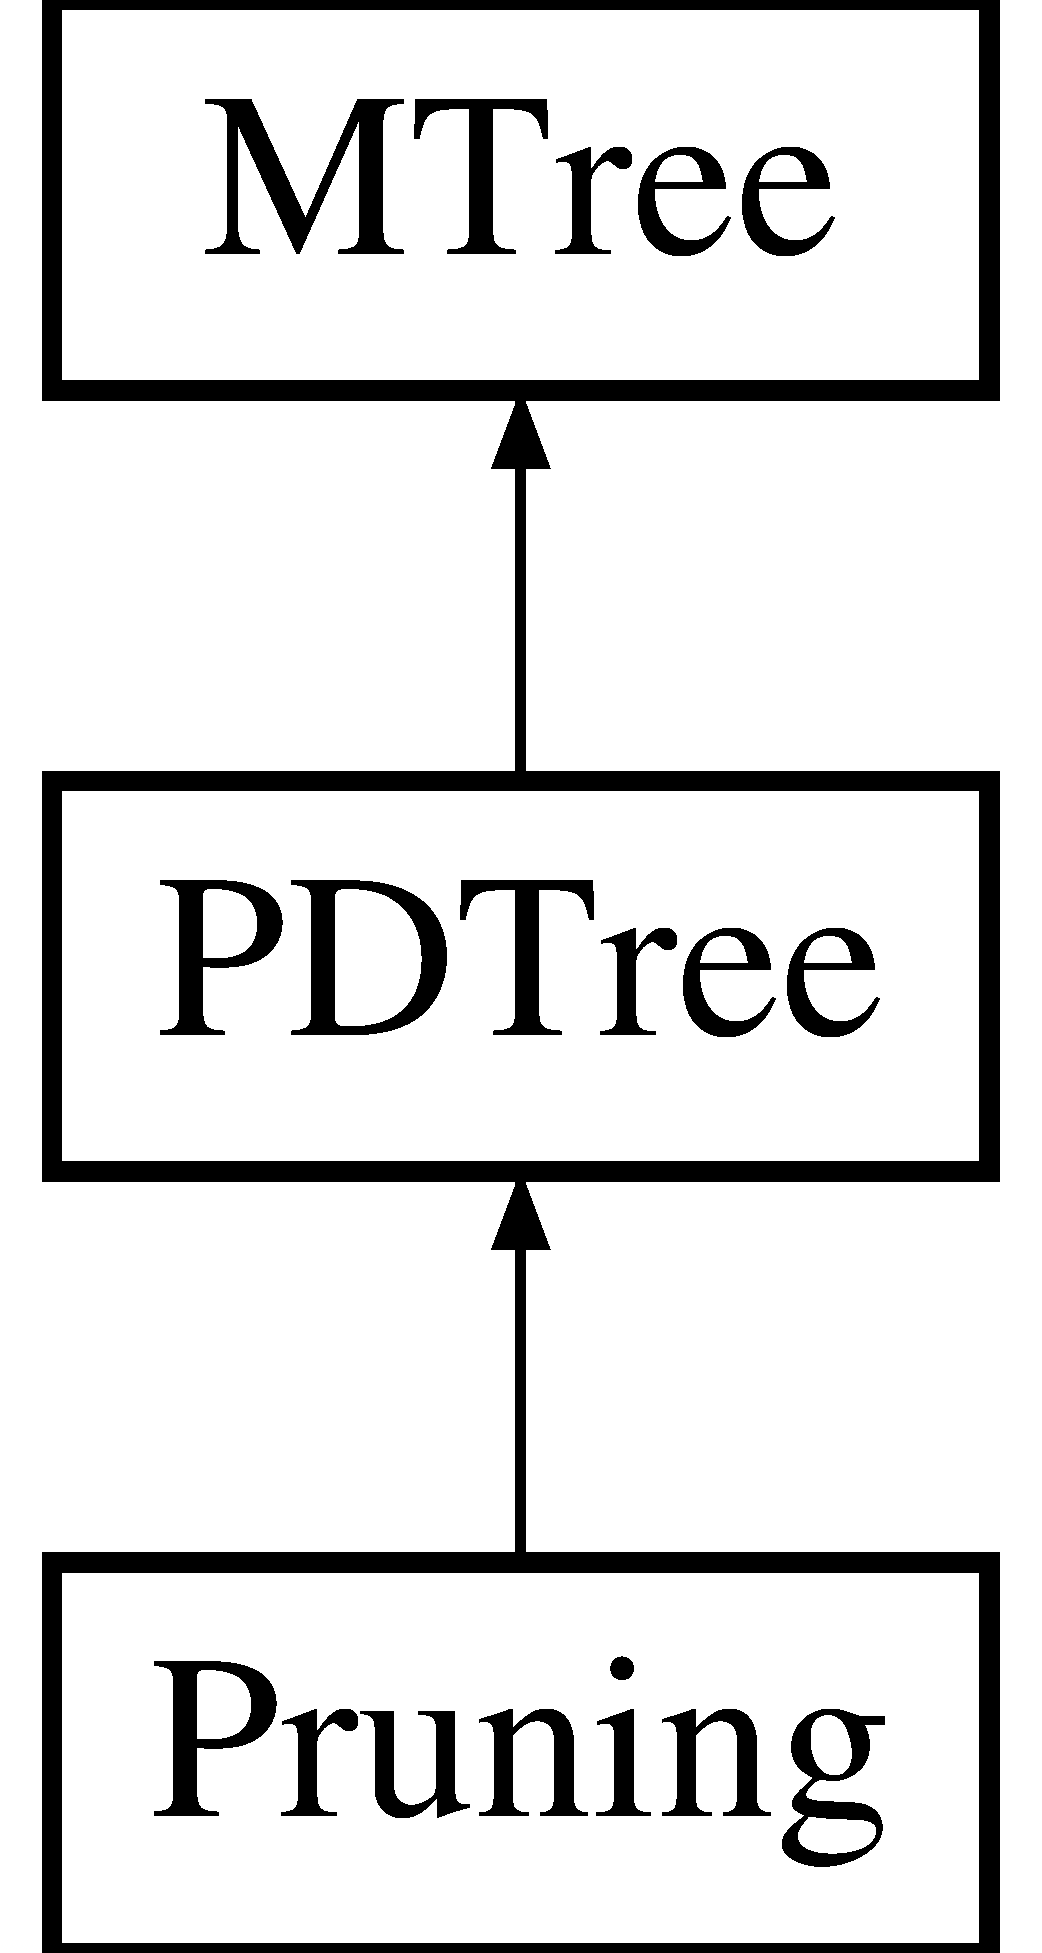
\includegraphics[height=3cm]{classPruning}
\end{center}
\end{figure}
\subsection*{Public Member Functions}
\begin{DoxyCompactItemize}
\item 
\hyperlink{classPruning_a020fa8f3cef1e1119e534c5b6f0c8fae}{Pruning} (\hyperlink{structParams}{Params} \&params)
\item 
\hyperlink{classPruning_a4dd4ec835b284391a7260e3cd6b4491d}{Pruning} (\hyperlink{classPDTree}{PDTree} \&tree)
\item 
\hyperlink{classPruning_a71d6f0210e5083b0eded402c165431b7}{Pruning} ()
\item 
void \hyperlink{classPruning_a9ee0d53c821bfca89ebe57f090eeba99}{run} (\hyperlink{structParams}{Params} \&params, vector$<$ \hyperlink{classPDTaxaSet}{PDTaxaSet} $>$ \&taxa\_\-set)
\item 
void \hyperlink{classPruning_ab3423a1002c0eb4af4568f9accac93fa}{deleteExNode} (LeafSet::iterator pos)
\item 
void \hyperlink{classPruning_aeb07f089da3792788648d2b8d7d702ca}{buildLeaves} (\hyperlink{classNode}{Node} $\ast$node=NULL, \hyperlink{classNode}{Node} $\ast$dad=NULL)
\item 
void \hyperlink{classPruning_ae0e583aa4e812cdce06af4cc634e0110}{printLeaves} ()
\item 
LeafSet::iterator \hyperlink{classPruning_a973dc17e371f5104adef79f4c227e81a}{findNode} (\hyperlink{classNode}{Node} $\ast$node)
\item 
LeafSet::iterator \hyperlink{classPruning_a9cf587b15c0bcabf01531a916d2338d5}{nearestLeaf} ()
\item 
void \hyperlink{classPruning_a03ad4c7dce2fee530783d4b783ac32e4}{doInitialSet} ()
\item 
void \hyperlink{classPruning_a6000133f6408dba298337f873dd1d165}{addLeaf} (\hyperlink{classNode}{Node} $\ast$leaf)
\end{DoxyCompactItemize}
\subsection*{Public Attributes}
\begin{DoxyCompactItemize}
\item 
LeafSet \hyperlink{classPruning_aa7b17e04be84e8605bef199af9c86656}{leaves}
\item 
int \hyperlink{classPruning_a0b7c9c3601f3facb5eeb9b40f4a11059}{list\_\-size}
\end{DoxyCompactItemize}


\subsection{Detailed Description}
Implementation of \hyperlink{classPruning}{Pruning} algorithm with complexity O(n$\ast$log(n-\/k))

\begin{DoxyAuthor}{Author}
BUI Quang Minh, Steffen Klaere, Arndt von Haeseler 
\end{DoxyAuthor}


\subsection{Constructor \& Destructor Documentation}
\hypertarget{classPruning_a020fa8f3cef1e1119e534c5b6f0c8fae}{
\index{Pruning@{Pruning}!Pruning@{Pruning}}
\index{Pruning@{Pruning}!Pruning@{Pruning}}
\subsubsection[{Pruning}]{\setlength{\rightskip}{0pt plus 5cm}Pruning::Pruning ({\bf Params} \& {\em params})\hspace{0.3cm}{\ttfamily  \mbox{[}inline\mbox{]}}}}
\label{classPruning_a020fa8f3cef1e1119e534c5b6f0c8fae}
construct from program parameters 
\begin{DoxyParams}{Parameters}
\item[{\em params}]program parameters \end{DoxyParams}
\hypertarget{classPruning_a4dd4ec835b284391a7260e3cd6b4491d}{
\index{Pruning@{Pruning}!Pruning@{Pruning}}
\index{Pruning@{Pruning}!Pruning@{Pruning}}
\subsubsection[{Pruning}]{\setlength{\rightskip}{0pt plus 5cm}Pruning::Pruning ({\bf PDTree} \& {\em tree})\hspace{0.3cm}{\ttfamily  \mbox{[}inline\mbox{]}}}}
\label{classPruning_a4dd4ec835b284391a7260e3cd6b4491d}
constructor, get from another tree 
\begin{DoxyParams}{Parameters}
\item[{\em tree}]another \hyperlink{classMTree}{MTree} \end{DoxyParams}
\hypertarget{classPruning_a71d6f0210e5083b0eded402c165431b7}{
\index{Pruning@{Pruning}!Pruning@{Pruning}}
\index{Pruning@{Pruning}!Pruning@{Pruning}}
\subsubsection[{Pruning}]{\setlength{\rightskip}{0pt plus 5cm}Pruning::Pruning ()\hspace{0.3cm}{\ttfamily  \mbox{[}inline\mbox{]}}}}
\label{classPruning_a71d6f0210e5083b0eded402c165431b7}
constructor 

\subsection{Member Function Documentation}
\hypertarget{classPruning_a6000133f6408dba298337f873dd1d165}{
\index{Pruning@{Pruning}!addLeaf@{addLeaf}}
\index{addLeaf@{addLeaf}!Pruning@{Pruning}}
\subsubsection[{addLeaf}]{\setlength{\rightskip}{0pt plus 5cm}void Pruning::addLeaf ({\bf Node} $\ast$ {\em leaf})}}
\label{classPruning_a6000133f6408dba298337f873dd1d165}
insert a leaf into the LeafSet 
\begin{DoxyParams}{Parameters}
\item[{\em leaf}]leaf node to be inserted\end{DoxyParams}
insert a leaf into the LeafSet \hypertarget{classPruning_aeb07f089da3792788648d2b8d7d702ca}{
\index{Pruning@{Pruning}!buildLeaves@{buildLeaves}}
\index{buildLeaves@{buildLeaves}!Pruning@{Pruning}}
\subsubsection[{buildLeaves}]{\setlength{\rightskip}{0pt plus 5cm}void Pruning::buildLeaves ({\bf Node} $\ast$ {\em node} = {\ttfamily NULL}, \/  {\bf Node} $\ast$ {\em dad} = {\ttfamily NULL})}}
\label{classPruning_aeb07f089da3792788648d2b8d7d702ca}
build the list of all leaves into field leaves. 
\begin{DoxyParams}{Parameters}
\item[{\em node}]the starting node, NULL to start from the root \item[{\em dad}]dad of the node, used to direct the search \end{DoxyParams}
\hypertarget{classPruning_ab3423a1002c0eb4af4568f9accac93fa}{
\index{Pruning@{Pruning}!deleteExNode@{deleteExNode}}
\index{deleteExNode@{deleteExNode}!Pruning@{Pruning}}
\subsubsection[{deleteExNode}]{\setlength{\rightskip}{0pt plus 5cm}void Pruning::deleteExNode (LeafSet::iterator {\em pos})}}
\label{classPruning_ab3423a1002c0eb4af4568f9accac93fa}
delete an external node 
\begin{DoxyParams}{Parameters}
\item[{\em pos}]the position of the node in the LeafSet \end{DoxyParams}
\hypertarget{classPruning_a03ad4c7dce2fee530783d4b783ac32e4}{
\index{Pruning@{Pruning}!doInitialSet@{doInitialSet}}
\index{doInitialSet@{doInitialSet}!Pruning@{Pruning}}
\subsubsection[{doInitialSet}]{\setlength{\rightskip}{0pt plus 5cm}void Pruning::doInitialSet ()}}
\label{classPruning_a03ad4c7dce2fee530783d4b783ac32e4}
mark the node in the inital set to be not PRUNABLE \hypertarget{classPruning_a973dc17e371f5104adef79f4c227e81a}{
\index{Pruning@{Pruning}!findNode@{findNode}}
\index{findNode@{findNode}!Pruning@{Pruning}}
\subsubsection[{findNode}]{\setlength{\rightskip}{0pt plus 5cm}LeafSet::iterator Pruning::findNode ({\bf Node} $\ast$ {\em node})}}
\label{classPruning_a973dc17e371f5104adef79f4c227e81a}
find the iterator to the leaf node in leaves field 
\begin{DoxyParams}{Parameters}
\item[{\em node}]a leaf node. \end{DoxyParams}
\begin{DoxyReturn}{Returns}
iterator to the leaf node in leaves field 
\end{DoxyReturn}
\hypertarget{classPruning_a9cf587b15c0bcabf01531a916d2338d5}{
\index{Pruning@{Pruning}!nearestLeaf@{nearestLeaf}}
\index{nearestLeaf@{nearestLeaf}!Pruning@{Pruning}}
\subsubsection[{nearestLeaf}]{\setlength{\rightskip}{0pt plus 5cm}LeafSet::iterator Pruning::nearestLeaf ()}}
\label{classPruning_a9cf587b15c0bcabf01531a916d2338d5}
\begin{DoxyReturn}{Returns}
leaves.begin(). 
\end{DoxyReturn}
\hypertarget{classPruning_ae0e583aa4e812cdce06af4cc634e0110}{
\index{Pruning@{Pruning}!printLeaves@{printLeaves}}
\index{printLeaves@{printLeaves}!Pruning@{Pruning}}
\subsubsection[{printLeaves}]{\setlength{\rightskip}{0pt plus 5cm}void Pruning::printLeaves ()}}
\label{classPruning_ae0e583aa4e812cdce06af4cc634e0110}
print all leaves into screen \hypertarget{classPruning_a9ee0d53c821bfca89ebe57f090eeba99}{
\index{Pruning@{Pruning}!run@{run}}
\index{run@{run}!Pruning@{Pruning}}
\subsubsection[{run}]{\setlength{\rightskip}{0pt plus 5cm}void Pruning::run ({\bf Params} \& {\em params}, \/  vector$<$ {\bf PDTaxaSet} $>$ \& {\em taxa\_\-set})}}
\label{classPruning_a9ee0d53c821bfca89ebe57f090eeba99}
run the algorithm 
\begin{DoxyParams}{Parameters}
\item[{\em params}]program parameters \item[{\em taxa\_\-set}](OUT) vector of PD sets\end{DoxyParams}
Steffen Klaere's pruning algorithm 

\subsection{Member Data Documentation}
\hypertarget{classPruning_aa7b17e04be84e8605bef199af9c86656}{
\index{Pruning@{Pruning}!leaves@{leaves}}
\index{leaves@{leaves}!Pruning@{Pruning}}
\subsubsection[{leaves}]{\setlength{\rightskip}{0pt plus 5cm}LeafSet {\bf Pruning::leaves}}}
\label{classPruning_aa7b17e04be84e8605bef199af9c86656}
leaf set of the tree, used for pruning algorithm \hypertarget{classPruning_a0b7c9c3601f3facb5eeb9b40f4a11059}{
\index{Pruning@{Pruning}!list\_\-size@{list\_\-size}}
\index{list\_\-size@{list\_\-size}!Pruning@{Pruning}}
\subsubsection[{list\_\-size}]{\setlength{\rightskip}{0pt plus 5cm}int {\bf Pruning::list\_\-size}}}
\label{classPruning_a0b7c9c3601f3facb5eeb9b40f4a11059}
maximum size of the ordered list of leaves 

The documentation for this class was generated from the following files:\begin{DoxyCompactItemize}
\item 
src/pruning.h\item 
src/pruning.cpp\end{DoxyCompactItemize}

\hypertarget{structPruningInfo}{
\section{PruningInfo Struct Reference}
\label{structPruningInfo}\index{PruningInfo@{PruningInfo}}
}
\subsection*{Public Attributes}
\begin{DoxyCompactItemize}
\item 
\hypertarget{structPruningInfo_a02d6eb38fbbdf135c7dcd6b43e9ac641}{
NeighborVec::iterator {\bfseries dad\_\-it\_\-left}}
\label{structPruningInfo_a02d6eb38fbbdf135c7dcd6b43e9ac641}

\item 
\hypertarget{structPruningInfo_ac0575205e6e906bbff240c2961246456}{
NeighborVec::iterator {\bfseries dad\_\-it\_\-right}}
\label{structPruningInfo_ac0575205e6e906bbff240c2961246456}

\item 
\hypertarget{structPruningInfo_a0dedf64569fe2b8ac4a1bff503667d46}{
NeighborVec::iterator {\bfseries left\_\-it}}
\label{structPruningInfo_a0dedf64569fe2b8ac4a1bff503667d46}

\item 
\hypertarget{structPruningInfo_a64882e04f5fc14dce56037aebaa29cdd}{
NeighborVec::iterator {\bfseries right\_\-it}}
\label{structPruningInfo_a64882e04f5fc14dce56037aebaa29cdd}

\item 
\hypertarget{structPruningInfo_af7052b9a2aaa8b57e2503b595adcd404}{
\hyperlink{classNeighbor}{Neighbor} $\ast$ {\bfseries dad\_\-nei\_\-left}}
\label{structPruningInfo_af7052b9a2aaa8b57e2503b595adcd404}

\item 
\hypertarget{structPruningInfo_a3c84954be0d5d9513782dc1b22c0f618}{
\hyperlink{classNeighbor}{Neighbor} $\ast$ {\bfseries dad\_\-nei\_\-right}}
\label{structPruningInfo_a3c84954be0d5d9513782dc1b22c0f618}

\item 
\hypertarget{structPruningInfo_a925d453486d7bac4b268779b84893f60}{
\hyperlink{classNeighbor}{Neighbor} $\ast$ {\bfseries left\_\-nei}}
\label{structPruningInfo_a925d453486d7bac4b268779b84893f60}

\item 
\hypertarget{structPruningInfo_aa34ac9fa1918c261d606279436e1b2b8}{
\hyperlink{classNeighbor}{Neighbor} $\ast$ {\bfseries right\_\-nei}}
\label{structPruningInfo_aa34ac9fa1918c261d606279436e1b2b8}

\item 
\hypertarget{structPruningInfo_a99285f9c2373612afe9695dbeae390d4}{
\hyperlink{classNode}{Node} $\ast$ {\bfseries node}}
\label{structPruningInfo_a99285f9c2373612afe9695dbeae390d4}

\item 
\hypertarget{structPruningInfo_adabe089d7a0af10ef05ae3a7c89efc7f}{
\hyperlink{classNode}{Node} $\ast$ {\bfseries dad}}
\label{structPruningInfo_adabe089d7a0af10ef05ae3a7c89efc7f}

\item 
\hypertarget{structPruningInfo_ad7fccd2c088de6e5dcf602d121bbf4b9}{
\hyperlink{classNode}{Node} $\ast$ {\bfseries left\_\-node}}
\label{structPruningInfo_ad7fccd2c088de6e5dcf602d121bbf4b9}

\item 
\hypertarget{structPruningInfo_a26cd0b6db39ff90d2d9eeae91072b357}{
\hyperlink{classNode}{Node} $\ast$ {\bfseries right\_\-node}}
\label{structPruningInfo_a26cd0b6db39ff90d2d9eeae91072b357}

\item 
\hypertarget{structPruningInfo_aa38d094382df0bf9332b7df30ca1dbaa}{
double {\bfseries left\_\-len}}
\label{structPruningInfo_aa38d094382df0bf9332b7df30ca1dbaa}

\item 
\hypertarget{structPruningInfo_ad707df4f786d3b69b28c37cd66861d8d}{
double {\bfseries right\_\-len}}
\label{structPruningInfo_ad707df4f786d3b69b28c37cd66861d8d}

\item 
\hypertarget{structPruningInfo_a07a4ea31a495780db8adc374ab8b4ac5}{
double $\ast$ {\bfseries dad\_\-lh\_\-left}}
\label{structPruningInfo_a07a4ea31a495780db8adc374ab8b4ac5}

\item 
\hypertarget{structPruningInfo_a49135d608f2f25ae7492080e07f04903}{
double $\ast$ {\bfseries dad\_\-lh\_\-right}}
\label{structPruningInfo_a49135d608f2f25ae7492080e07f04903}

\end{DoxyCompactItemize}


The documentation for this struct was generated from the following file:\begin{DoxyCompactItemize}
\item 
src/phylotree.h\end{DoxyCompactItemize}

\hypertarget{classRateGamma}{
\section{RateGamma Class Reference}
\label{classRateGamma}\index{RateGamma@{RateGamma}}
}


{\ttfamily \#include $<$rategamma.h$>$}Inheritance diagram for RateGamma::\begin{figure}[H]
\begin{center}
\leavevmode
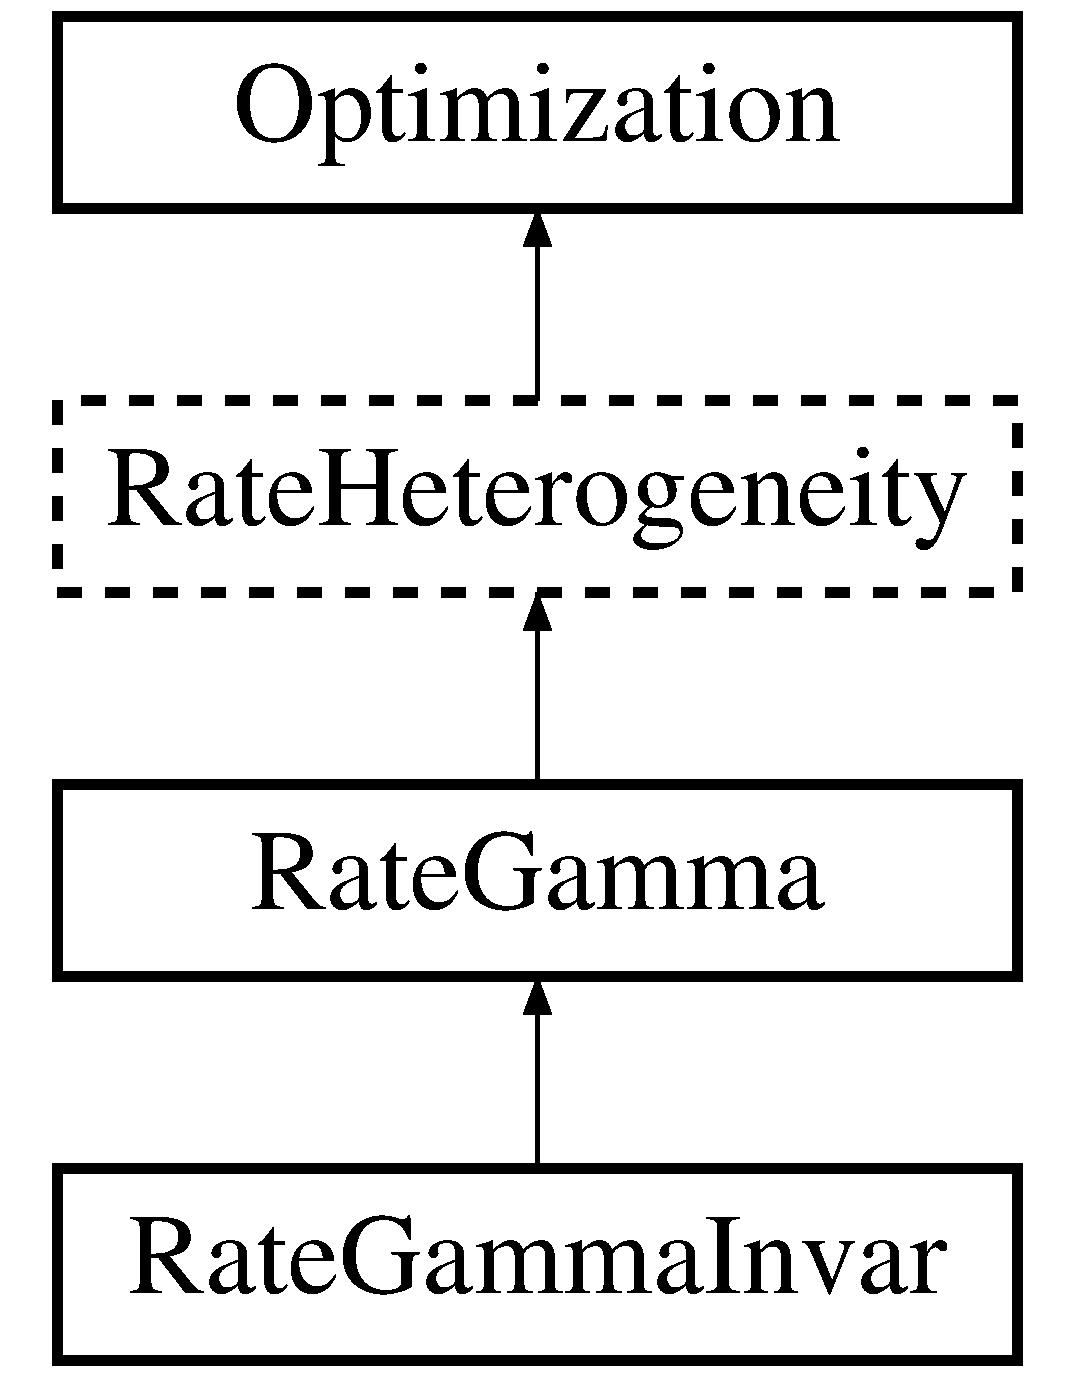
\includegraphics[height=4cm]{classRateGamma}
\end{center}
\end{figure}
\subsection*{Public Member Functions}
\begin{DoxyCompactItemize}
\item 
\hyperlink{classRateGamma_a040b97ec98732b29809b6cd03055b441}{RateGamma} (int ncat, \hyperlink{classPhyloTree}{PhyloTree} $\ast$tree)
\item 
virtual \hyperlink{classRateGamma_a5989cd3261ba9ae18d3fd23f532b74e2}{$\sim$RateGamma} ()
\item 
virtual int \hyperlink{classRateGamma_a115dac63aaa8fc7ac256304506ef3307}{getNRate} ()
\item 
virtual double \hyperlink{classRateGamma_a2e459469fd578b9d5d8bb18000d9d1d9}{getRate} (int category)
\item 
void \hyperlink{classRateGamma_a487fec4116b061846ec8cf1dd5d5b43f}{computeRates} ()
\item 
virtual double \hyperlink{classRateGamma_aadba870d743295ef057f9c78ac7fdd06}{optimizeParameters} ()
\item 
virtual double \hyperlink{classRateGamma_a24e01b7ec0d9170ceebcf03b603b2bbb}{computeFunction} (double shape)
\item 
virtual int \hyperlink{classRateGamma_af271c0115c8a81ff6fac32d1cfef6187}{getNDim} ()
\item 
virtual void \hyperlink{classRateGamma_a835bb210fd8fb4552613fe49875cbfb5}{writeInfo} (ostream \&out)
\item 
virtual void \hyperlink{classRateGamma_a88ffb33131f2cf23cfd0525e092c7717}{writeParameters} (ostream \&out)
\end{DoxyCompactItemize}
\subsection*{Protected Member Functions}
\begin{DoxyCompactItemize}
\item 
\hypertarget{classRateGamma_af08e1d7ff25ba462357db3f019617658}{
double {\bfseries cmpPerPointGamma} (const double prob, const double shape)}
\label{classRateGamma_af08e1d7ff25ba462357db3f019617658}

\item 
double \hyperlink{classRateGamma_a10e81681fe39582f6ed6c89b554fbeab}{cmpLnGamma} (double alpha)
\item 
double \hyperlink{classRateGamma_a30b08c43d6ca5266a801b825baa3ac1f}{cmpIncompleteGamma} (double x, double alpha, double ln\_\-gamma\_\-alpha)
\item 
double \hyperlink{classRateGamma_a65fda804b83f71c65b365c16a6e01e4b}{cmpPointNormal} (double prob)
\item 
double \hyperlink{classRateGamma_ac7740803fb3a31189a17d9173848774b}{cmpPointChi2} (double prob, double v)
\end{DoxyCompactItemize}
\subsection*{Protected Attributes}
\begin{DoxyCompactItemize}
\item 
int \hyperlink{classRateGamma_adeaf25f809c07e9fdf368bece8190900}{ncategory}
\item 
double $\ast$ \hyperlink{classRateGamma_a9f72703c81eb78da12198c44fcf7d68c}{rates}
\item 
double \hyperlink{classRateGamma_a88433a75c040757da67d9007c2ab9db4}{gamma\_\-shape}
\end{DoxyCompactItemize}


\subsection{Detailed Description}
Discrete gamma distributed site-\/rate model from Yang 1994

\begin{DoxyAuthor}{Author}
BUI Quang Minh $<$\href{mailto:minh.bui@univie.ac.at}{\tt minh.bui@univie.ac.at}$>$ 
\end{DoxyAuthor}


\subsection{Constructor \& Destructor Documentation}
\hypertarget{classRateGamma_a040b97ec98732b29809b6cd03055b441}{
\index{RateGamma@{RateGamma}!RateGamma@{RateGamma}}
\index{RateGamma@{RateGamma}!RateGamma@{RateGamma}}
\subsubsection[{RateGamma}]{\setlength{\rightskip}{0pt plus 5cm}RateGamma::RateGamma (int {\em ncat}, \/  {\bf PhyloTree} $\ast$ {\em tree})}}
\label{classRateGamma_a040b97ec98732b29809b6cd03055b441}
constructor 
\begin{DoxyParams}{Parameters}
\item[{\em ncat}]number of rate categories \item[{\em tree}]associated phylogenetic tree \end{DoxyParams}
\hypertarget{classRateGamma_a5989cd3261ba9ae18d3fd23f532b74e2}{
\index{RateGamma@{RateGamma}!$\sim$RateGamma@{$\sim$RateGamma}}
\index{$\sim$RateGamma@{$\sim$RateGamma}!RateGamma@{RateGamma}}
\subsubsection[{$\sim$RateGamma}]{\setlength{\rightskip}{0pt plus 5cm}RateGamma::$\sim$RateGamma ()\hspace{0.3cm}{\ttfamily  \mbox{[}virtual\mbox{]}}}}
\label{classRateGamma_a5989cd3261ba9ae18d3fd23f532b74e2}
destructor 

\subsection{Member Function Documentation}
\hypertarget{classRateGamma_a30b08c43d6ca5266a801b825baa3ac1f}{
\index{RateGamma@{RateGamma}!cmpIncompleteGamma@{cmpIncompleteGamma}}
\index{cmpIncompleteGamma@{cmpIncompleteGamma}!RateGamma@{RateGamma}}
\subsubsection[{cmpIncompleteGamma}]{\setlength{\rightskip}{0pt plus 5cm}double RateGamma::cmpIncompleteGamma (double {\em x}, \/  double {\em alpha}, \/  double {\em ln\_\-gamma\_\-alpha})\hspace{0.3cm}{\ttfamily  \mbox{[}protected\mbox{]}}}}
\label{classRateGamma_a30b08c43d6ca5266a801b825baa3ac1f}
returns the incomplete gamma ratio I(x,alpha) where x is the upper limit of the integration and alpha is the shape parameter. returns (-\/1) if in error (1) series expansion if (alpha$>$x $|$$|$ x$<$=1) (2) continued fraction otherwise RATNEST FORTRAN by Bhattacharjee GP (1970) The incomplete gamma integral. Applied Statistics, 19: 285-\/287 (AS32) \hypertarget{classRateGamma_a10e81681fe39582f6ed6c89b554fbeab}{
\index{RateGamma@{RateGamma}!cmpLnGamma@{cmpLnGamma}}
\index{cmpLnGamma@{cmpLnGamma}!RateGamma@{RateGamma}}
\subsubsection[{cmpLnGamma}]{\setlength{\rightskip}{0pt plus 5cm}double RateGamma::cmpLnGamma (double {\em alpha})\hspace{0.3cm}{\ttfamily  \mbox{[}protected\mbox{]}}}}
\label{classRateGamma_a10e81681fe39582f6ed6c89b554fbeab}
returns ln(gamma(alpha)) for alpha$>$0, accurate to 10 decimal places. Stirling's formula is used for the central polynomial part of the procedure. Pike MC \& Hill ID (1966) Algorithm 291: Logarithm of the gamma function. Communications of the Association for Computing Machinery, 9:684 \hypertarget{classRateGamma_ac7740803fb3a31189a17d9173848774b}{
\index{RateGamma@{RateGamma}!cmpPointChi2@{cmpPointChi2}}
\index{cmpPointChi2@{cmpPointChi2}!RateGamma@{RateGamma}}
\subsubsection[{cmpPointChi2}]{\setlength{\rightskip}{0pt plus 5cm}double RateGamma::cmpPointChi2 (double {\em prob}, \/  double {\em v})\hspace{0.3cm}{\ttfamily  \mbox{[}protected\mbox{]}}}}
\label{classRateGamma_ac7740803fb3a31189a17d9173848774b}
returns z so that Prob\{x$<$z\}=prob where x is Chi2 distributed with df=v returns -\/1 if in error. 0.000002$<$prob$<$0.999998 RATNEST FORTRAN by Best DJ \& Roberts DE (1975) The percentage points of the Chi2 distribution. Applied Statistics 24: 385-\/388. (AS91) Converted into C by Ziheng Yang, Oct. 1993. \hypertarget{classRateGamma_a65fda804b83f71c65b365c16a6e01e4b}{
\index{RateGamma@{RateGamma}!cmpPointNormal@{cmpPointNormal}}
\index{cmpPointNormal@{cmpPointNormal}!RateGamma@{RateGamma}}
\subsubsection[{cmpPointNormal}]{\setlength{\rightskip}{0pt plus 5cm}double RateGamma::cmpPointNormal (double {\em prob})\hspace{0.3cm}{\ttfamily  \mbox{[}protected\mbox{]}}}}
\label{classRateGamma_a65fda804b83f71c65b365c16a6e01e4b}
functions concerning the CDF and percentage points of the gamma and Chi2 distribution returns z so that Prob\{x$<$z\}=prob where x $\sim$ N(0,1) and (1e-\/12)$<$prob$<$1-\/(1e-\/12) returns (-\/9999) if in error Odeh RE \& Evans JO (1974) The percentage points of the normal distribution. Applied Statistics 22: 96-\/97 (AS70)

Newer methods: Wichura MJ (1988) Algorithm AS 241: the percentage points of the normal distribution. 37: 477-\/484. Beasley JD \& Springer SG (1977). Algorithm AS 111: the percentage points of the normal distribution. 26: 118-\/121. \hypertarget{classRateGamma_a24e01b7ec0d9170ceebcf03b603b2bbb}{
\index{RateGamma@{RateGamma}!computeFunction@{computeFunction}}
\index{computeFunction@{computeFunction}!RateGamma@{RateGamma}}
\subsubsection[{computeFunction}]{\setlength{\rightskip}{0pt plus 5cm}double RateGamma::computeFunction (double {\em shape})\hspace{0.3cm}{\ttfamily  \mbox{[}virtual\mbox{]}}}}
\label{classRateGamma_a24e01b7ec0d9170ceebcf03b603b2bbb}
override function from \hyperlink{classOptimization}{Optimization} class, used by the \hyperlink{classOptimization_a59ccdfae81744716ce48226da029d470}{minimizeOneDimen()} to optimize gamma shape parameter 

Reimplemented from \hyperlink{classOptimization_ad7ca7b884076f8c76312d516e23c6609}{Optimization}.

Reimplemented in \hyperlink{classRateGammaInvar_a48fde92a023867c5d0656572f8dc0f71}{RateGammaInvar}.\hypertarget{classRateGamma_a487fec4116b061846ec8cf1dd5d5b43f}{
\index{RateGamma@{RateGamma}!computeRates@{computeRates}}
\index{computeRates@{computeRates}!RateGamma@{RateGamma}}
\subsubsection[{computeRates}]{\setlength{\rightskip}{0pt plus 5cm}void RateGamma::computeRates ()}}
\label{classRateGamma_a487fec4116b061846ec8cf1dd5d5b43f}
discrete Gamma according to Yang 1994 (JME 39:306-\/314). It takes 'ncategory' and 'gamma\_\-shape' variables as input. On output, it write to 'rates' variable. \hypertarget{classRateGamma_af271c0115c8a81ff6fac32d1cfef6187}{
\index{RateGamma@{RateGamma}!getNDim@{getNDim}}
\index{getNDim@{getNDim}!RateGamma@{RateGamma}}
\subsubsection[{getNDim}]{\setlength{\rightskip}{0pt plus 5cm}virtual int RateGamma::getNDim ()\hspace{0.3cm}{\ttfamily  \mbox{[}inline, virtual\mbox{]}}}}
\label{classRateGamma_af271c0115c8a81ff6fac32d1cfef6187}
return the number of dimensions 

Reimplemented from \hyperlink{classOptimization_a6d04cefb0969f3cac9b607aa1412eb57}{Optimization}.

Reimplemented in \hyperlink{classRateGammaInvar_a4f276d1639a79eece217b365439049c7}{RateGammaInvar}.\hypertarget{classRateGamma_a115dac63aaa8fc7ac256304506ef3307}{
\index{RateGamma@{RateGamma}!getNRate@{getNRate}}
\index{getNRate@{getNRate}!RateGamma@{RateGamma}}
\subsubsection[{getNRate}]{\setlength{\rightskip}{0pt plus 5cm}virtual int RateGamma::getNRate ()\hspace{0.3cm}{\ttfamily  \mbox{[}inline, virtual\mbox{]}}}}
\label{classRateGamma_a115dac63aaa8fc7ac256304506ef3307}
\begin{DoxyReturn}{Returns}
the number of rate categories 
\end{DoxyReturn}


Reimplemented from \hyperlink{classRateHeterogeneity_ac61808650eab5d2187f3cc9b20694f80}{RateHeterogeneity}.\hypertarget{classRateGamma_a2e459469fd578b9d5d8bb18000d9d1d9}{
\index{RateGamma@{RateGamma}!getRate@{getRate}}
\index{getRate@{getRate}!RateGamma@{RateGamma}}
\subsubsection[{getRate}]{\setlength{\rightskip}{0pt plus 5cm}virtual double RateGamma::getRate (int {\em category})\hspace{0.3cm}{\ttfamily  \mbox{[}inline, virtual\mbox{]}}}}
\label{classRateGamma_a2e459469fd578b9d5d8bb18000d9d1d9}

\begin{DoxyParams}{Parameters}
\item[{\em category}]category ID from 0 to category-\/1 \end{DoxyParams}
\begin{DoxyReturn}{Returns}
the rate of the specified category 
\end{DoxyReturn}


Reimplemented from \hyperlink{classRateHeterogeneity_a87546419c324a62d31055d564ea07f5e}{RateHeterogeneity}.\hypertarget{classRateGamma_aadba870d743295ef057f9c78ac7fdd06}{
\index{RateGamma@{RateGamma}!optimizeParameters@{optimizeParameters}}
\index{optimizeParameters@{optimizeParameters}!RateGamma@{RateGamma}}
\subsubsection[{optimizeParameters}]{\setlength{\rightskip}{0pt plus 5cm}double RateGamma::optimizeParameters ()\hspace{0.3cm}{\ttfamily  \mbox{[}virtual\mbox{]}}}}
\label{classRateGamma_aadba870d743295ef057f9c78ac7fdd06}
optimize parameters. Default is to optimize gamma shape \begin{DoxyReturn}{Returns}
the best likelihood 
\end{DoxyReturn}


Reimplemented from \hyperlink{classRateHeterogeneity_a1305d5b8481dd5a2482917ddb5fe57bd}{RateHeterogeneity}.

Reimplemented in \hyperlink{classRateGammaInvar_ab72a2559cea978d312a243d521c2abef}{RateGammaInvar}.\hypertarget{classRateGamma_a835bb210fd8fb4552613fe49875cbfb5}{
\index{RateGamma@{RateGamma}!writeInfo@{writeInfo}}
\index{writeInfo@{writeInfo}!RateGamma@{RateGamma}}
\subsubsection[{writeInfo}]{\setlength{\rightskip}{0pt plus 5cm}void RateGamma::writeInfo (ostream \& {\em out})\hspace{0.3cm}{\ttfamily  \mbox{[}virtual\mbox{]}}}}
\label{classRateGamma_a835bb210fd8fb4552613fe49875cbfb5}
write information 
\begin{DoxyParams}{Parameters}
\item[{\em out}]output stream \end{DoxyParams}


Reimplemented from \hyperlink{classRateHeterogeneity_a520772859d465036b6620bdbf2977efe}{RateHeterogeneity}.

Reimplemented in \hyperlink{classRateGammaInvar_a428c3ac79ba1bf28da546f602d4b0f7b}{RateGammaInvar}.\hypertarget{classRateGamma_a88ffb33131f2cf23cfd0525e092c7717}{
\index{RateGamma@{RateGamma}!writeParameters@{writeParameters}}
\index{writeParameters@{writeParameters}!RateGamma@{RateGamma}}
\subsubsection[{writeParameters}]{\setlength{\rightskip}{0pt plus 5cm}void RateGamma::writeParameters (ostream \& {\em out})\hspace{0.3cm}{\ttfamily  \mbox{[}virtual\mbox{]}}}}
\label{classRateGamma_a88ffb33131f2cf23cfd0525e092c7717}
write parameters, used with modeltest 
\begin{DoxyParams}{Parameters}
\item[{\em out}]output stream \end{DoxyParams}


Reimplemented from \hyperlink{classRateHeterogeneity_ad2832e686971cf1f2cac2a6f842a3550}{RateHeterogeneity}.

Reimplemented in \hyperlink{classRateGammaInvar_a13b6629de9e3579aacff555f1bd76db5}{RateGammaInvar}.

\subsection{Member Data Documentation}
\hypertarget{classRateGamma_a88433a75c040757da67d9007c2ab9db4}{
\index{RateGamma@{RateGamma}!gamma\_\-shape@{gamma\_\-shape}}
\index{gamma\_\-shape@{gamma\_\-shape}!RateGamma@{RateGamma}}
\subsubsection[{gamma\_\-shape}]{\setlength{\rightskip}{0pt plus 5cm}double {\bf RateGamma::gamma\_\-shape}\hspace{0.3cm}{\ttfamily  \mbox{[}protected\mbox{]}}}}
\label{classRateGamma_a88433a75c040757da67d9007c2ab9db4}
the gamma shape parameter 'alpha' \hypertarget{classRateGamma_adeaf25f809c07e9fdf368bece8190900}{
\index{RateGamma@{RateGamma}!ncategory@{ncategory}}
\index{ncategory@{ncategory}!RateGamma@{RateGamma}}
\subsubsection[{ncategory}]{\setlength{\rightskip}{0pt plus 5cm}int {\bf RateGamma::ncategory}\hspace{0.3cm}{\ttfamily  \mbox{[}protected\mbox{]}}}}
\label{classRateGamma_adeaf25f809c07e9fdf368bece8190900}
number of rate categories \hypertarget{classRateGamma_a9f72703c81eb78da12198c44fcf7d68c}{
\index{RateGamma@{RateGamma}!rates@{rates}}
\index{rates@{rates}!RateGamma@{RateGamma}}
\subsubsection[{rates}]{\setlength{\rightskip}{0pt plus 5cm}double$\ast$ {\bf RateGamma::rates}\hspace{0.3cm}{\ttfamily  \mbox{[}protected\mbox{]}}}}
\label{classRateGamma_a9f72703c81eb78da12198c44fcf7d68c}
rates, containing ncategory elements 

The documentation for this class was generated from the following files:\begin{DoxyCompactItemize}
\item 
src/rategamma.h\item 
src/rategamma.cpp\end{DoxyCompactItemize}

\hypertarget{classRateGammaInvar}{
\section{RateGammaInvar Class Reference}
\label{classRateGammaInvar}\index{RateGammaInvar@{RateGammaInvar}}
}


{\ttfamily \#include $<$rategammainvar.h$>$}Inheritance diagram for RateGammaInvar::\begin{figure}[H]
\begin{center}
\leavevmode
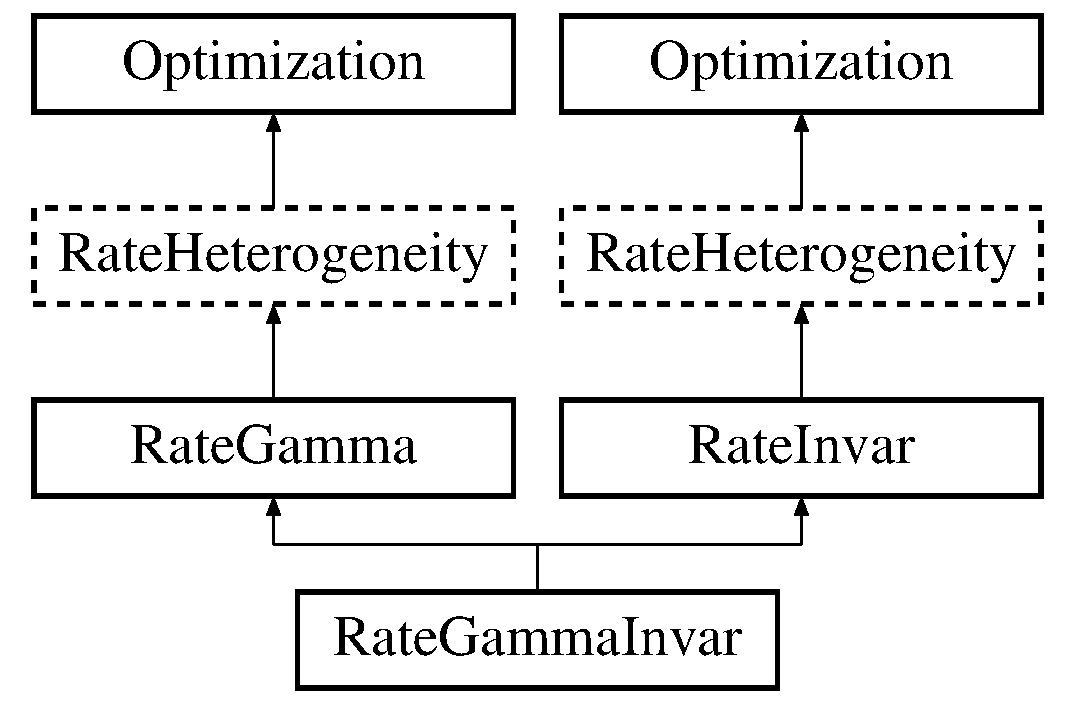
\includegraphics[height=4cm]{classRateGammaInvar}
\end{center}
\end{figure}
\subsection*{Public Member Functions}
\begin{DoxyCompactItemize}
\item 
\hyperlink{classRateGammaInvar_ada238d8306a13a7a9ad57fcb88349e48}{RateGammaInvar} (int ncat, \hyperlink{classPhyloTree}{PhyloTree} $\ast$tree)
\item 
virtual double \hyperlink{classRateGammaInvar_a48fde92a023867c5d0656572f8dc0f71}{computeFunction} (double value)
\item 
virtual double \hyperlink{classRateGammaInvar_ab72a2559cea978d312a243d521c2abef}{optimizeParameters} ()
\item 
virtual int \hyperlink{classRateGammaInvar_a4f276d1639a79eece217b365439049c7}{getNDim} ()
\item 
virtual void \hyperlink{classRateGammaInvar_a428c3ac79ba1bf28da546f602d4b0f7b}{writeInfo} (ostream \&out)
\item 
virtual void \hyperlink{classRateGammaInvar_a13b6629de9e3579aacff555f1bd76db5}{writeParameters} (ostream \&out)
\end{DoxyCompactItemize}


\subsection{Detailed Description}
class for I+G rate heterogeneity

\begin{DoxyAuthor}{Author}
BUI Quang Minh $<$\href{mailto:minh.bui@univie.ac.at}{\tt minh.bui@univie.ac.at}$>$ 
\end{DoxyAuthor}


\subsection{Constructor \& Destructor Documentation}
\hypertarget{classRateGammaInvar_ada238d8306a13a7a9ad57fcb88349e48}{
\index{RateGammaInvar@{RateGammaInvar}!RateGammaInvar@{RateGammaInvar}}
\index{RateGammaInvar@{RateGammaInvar}!RateGammaInvar@{RateGammaInvar}}
\subsubsection[{RateGammaInvar}]{\setlength{\rightskip}{0pt plus 5cm}RateGammaInvar::RateGammaInvar (int {\em ncat}, \/  {\bf PhyloTree} $\ast$ {\em tree})}}
\label{classRateGammaInvar_ada238d8306a13a7a9ad57fcb88349e48}
constructor 
\begin{DoxyParams}{Parameters}
\item[{\em ncat}]number of rate categories \item[{\em tree}]associated phylogenetic tree \end{DoxyParams}


\subsection{Member Function Documentation}
\hypertarget{classRateGammaInvar_a48fde92a023867c5d0656572f8dc0f71}{
\index{RateGammaInvar@{RateGammaInvar}!computeFunction@{computeFunction}}
\index{computeFunction@{computeFunction}!RateGammaInvar@{RateGammaInvar}}
\subsubsection[{computeFunction}]{\setlength{\rightskip}{0pt plus 5cm}double RateGammaInvar::computeFunction (double {\em value})\hspace{0.3cm}{\ttfamily  \mbox{[}virtual\mbox{]}}}}
\label{classRateGammaInvar_a48fde92a023867c5d0656572f8dc0f71}
override function from \hyperlink{classOptimization}{Optimization} class, used by the \hyperlink{classOptimization_a59ccdfae81744716ce48226da029d470}{minimizeOneDimen()} to optimize p\_\-invar or gamma shape parameter. 
\begin{DoxyParams}{Parameters}
\item[{\em value}]value of p\_\-invar (if cur\_\-optimize == 1) or gamma shape (if cur\_\-optimize == 0). \end{DoxyParams}


Reimplemented from \hyperlink{classRateGamma_a24e01b7ec0d9170ceebcf03b603b2bbb}{RateGamma}.\hypertarget{classRateGammaInvar_a4f276d1639a79eece217b365439049c7}{
\index{RateGammaInvar@{RateGammaInvar}!getNDim@{getNDim}}
\index{getNDim@{getNDim}!RateGammaInvar@{RateGammaInvar}}
\subsubsection[{getNDim}]{\setlength{\rightskip}{0pt plus 5cm}virtual int RateGammaInvar::getNDim ()\hspace{0.3cm}{\ttfamily  \mbox{[}inline, virtual\mbox{]}}}}
\label{classRateGammaInvar_a4f276d1639a79eece217b365439049c7}
return the number of dimensions 

Reimplemented from \hyperlink{classRateGamma_af271c0115c8a81ff6fac32d1cfef6187}{RateGamma}.\hypertarget{classRateGammaInvar_ab72a2559cea978d312a243d521c2abef}{
\index{RateGammaInvar@{RateGammaInvar}!optimizeParameters@{optimizeParameters}}
\index{optimizeParameters@{optimizeParameters}!RateGammaInvar@{RateGammaInvar}}
\subsubsection[{optimizeParameters}]{\setlength{\rightskip}{0pt plus 5cm}double RateGammaInvar::optimizeParameters ()\hspace{0.3cm}{\ttfamily  \mbox{[}virtual\mbox{]}}}}
\label{classRateGammaInvar_ab72a2559cea978d312a243d521c2abef}
optimize parameters \begin{DoxyReturn}{Returns}
the best likelihood 
\end{DoxyReturn}


Reimplemented from \hyperlink{classRateGamma_aadba870d743295ef057f9c78ac7fdd06}{RateGamma}.\hypertarget{classRateGammaInvar_a428c3ac79ba1bf28da546f602d4b0f7b}{
\index{RateGammaInvar@{RateGammaInvar}!writeInfo@{writeInfo}}
\index{writeInfo@{writeInfo}!RateGammaInvar@{RateGammaInvar}}
\subsubsection[{writeInfo}]{\setlength{\rightskip}{0pt plus 5cm}void RateGammaInvar::writeInfo (ostream \& {\em out})\hspace{0.3cm}{\ttfamily  \mbox{[}virtual\mbox{]}}}}
\label{classRateGammaInvar_a428c3ac79ba1bf28da546f602d4b0f7b}
write information 
\begin{DoxyParams}{Parameters}
\item[{\em out}]output stream \end{DoxyParams}


Reimplemented from \hyperlink{classRateGamma_a835bb210fd8fb4552613fe49875cbfb5}{RateGamma}.\hypertarget{classRateGammaInvar_a13b6629de9e3579aacff555f1bd76db5}{
\index{RateGammaInvar@{RateGammaInvar}!writeParameters@{writeParameters}}
\index{writeParameters@{writeParameters}!RateGammaInvar@{RateGammaInvar}}
\subsubsection[{writeParameters}]{\setlength{\rightskip}{0pt plus 5cm}void RateGammaInvar::writeParameters (ostream \& {\em out})\hspace{0.3cm}{\ttfamily  \mbox{[}virtual\mbox{]}}}}
\label{classRateGammaInvar_a13b6629de9e3579aacff555f1bd76db5}
write parameters, used with modeltest 
\begin{DoxyParams}{Parameters}
\item[{\em out}]output stream \end{DoxyParams}


Reimplemented from \hyperlink{classRateGamma_a88ffb33131f2cf23cfd0525e092c7717}{RateGamma}.

The documentation for this class was generated from the following files:\begin{DoxyCompactItemize}
\item 
src/rategammainvar.h\item 
src/rategammainvar.cpp\end{DoxyCompactItemize}

\hypertarget{classRateHeterogeneity}{
\section{RateHeterogeneity Class Reference}
\label{classRateHeterogeneity}\index{RateHeterogeneity@{RateHeterogeneity}}
}


{\ttfamily \#include $<$rateheterogeneity.h$>$}Inheritance diagram for RateHeterogeneity::\begin{figure}[H]
\begin{center}
\leavevmode
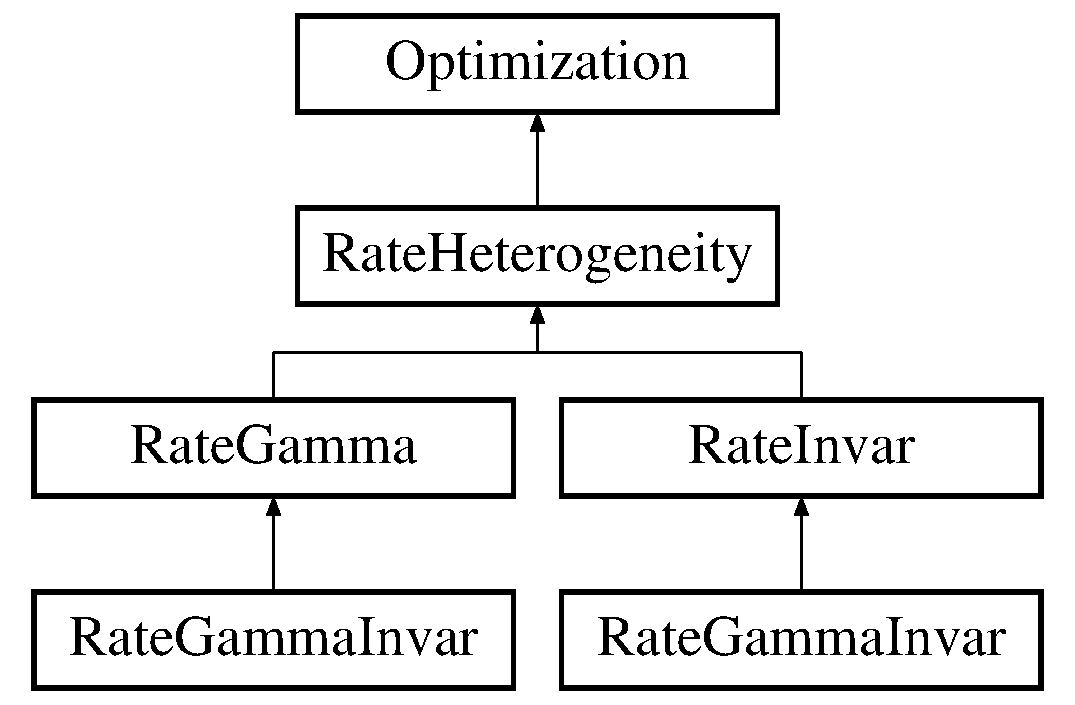
\includegraphics[height=4cm]{classRateHeterogeneity}
\end{center}
\end{figure}
\subsection*{Public Member Functions}
\begin{DoxyCompactItemize}
\item 
\hyperlink{classRateHeterogeneity_a9a1e70b493cfd7ce53bfbce242bbcb46}{RateHeterogeneity} ()
\item 
virtual \hyperlink{classRateHeterogeneity_a695587b35c973b88c6d669dd00ffd791}{$\sim$RateHeterogeneity} ()
\item 
void \hyperlink{classRateHeterogeneity_a5333e4d51b14b79dbaa32df641891cbb}{setTree} (\hyperlink{classPhyloTree}{PhyloTree} $\ast$tree)
\item 
virtual int \hyperlink{classRateHeterogeneity_ac61808650eab5d2187f3cc9b20694f80}{getNRate} ()
\item 
virtual double \hyperlink{classRateHeterogeneity_a87546419c324a62d31055d564ea07f5e}{getRate} (int category)
\item 
virtual double \hyperlink{classRateHeterogeneity_ada76d84ed7f66ddde02734d9c72f4e7b}{getPInvar} ()
\item 
virtual double \hyperlink{classRateHeterogeneity_a1305d5b8481dd5a2482917ddb5fe57bd}{optimizeParameters} ()
\item 
virtual void \hyperlink{classRateHeterogeneity_a520772859d465036b6620bdbf2977efe}{writeInfo} (ostream \&out)
\item 
virtual void \hyperlink{classRateHeterogeneity_ad2832e686971cf1f2cac2a6f842a3550}{writeParameters} (ostream \&out)
\end{DoxyCompactItemize}
\subsection*{Public Attributes}
\begin{DoxyCompactItemize}
\item 
string \hyperlink{classRateHeterogeneity_aec54d9090abff011fb0c437d51b1d759}{name}
\end{DoxyCompactItemize}
\subsection*{Protected Attributes}
\begin{DoxyCompactItemize}
\item 
\hyperlink{classPhyloTree}{PhyloTree} $\ast$ \hyperlink{classRateHeterogeneity_a15901cd491ded27a2d8cd4ddb731e647}{phylo\_\-tree}
\end{DoxyCompactItemize}


\subsection{Detailed Description}
class for among-\/site rate heterogeneity, the default is homogeneous (equal) rate model

\begin{DoxyAuthor}{Author}
BUI Quang Minh $<$\href{mailto:minh.bui@univie.ac.at}{\tt minh.bui@univie.ac.at}$>$ 
\end{DoxyAuthor}


\subsection{Constructor \& Destructor Documentation}
\hypertarget{classRateHeterogeneity_a9a1e70b493cfd7ce53bfbce242bbcb46}{
\index{RateHeterogeneity@{RateHeterogeneity}!RateHeterogeneity@{RateHeterogeneity}}
\index{RateHeterogeneity@{RateHeterogeneity}!RateHeterogeneity@{RateHeterogeneity}}
\subsubsection[{RateHeterogeneity}]{\setlength{\rightskip}{0pt plus 5cm}RateHeterogeneity::RateHeterogeneity ()}}
\label{classRateHeterogeneity_a9a1e70b493cfd7ce53bfbce242bbcb46}
constructor \hypertarget{classRateHeterogeneity_a695587b35c973b88c6d669dd00ffd791}{
\index{RateHeterogeneity@{RateHeterogeneity}!$\sim$RateHeterogeneity@{$\sim$RateHeterogeneity}}
\index{$\sim$RateHeterogeneity@{$\sim$RateHeterogeneity}!RateHeterogeneity@{RateHeterogeneity}}
\subsubsection[{$\sim$RateHeterogeneity}]{\setlength{\rightskip}{0pt plus 5cm}RateHeterogeneity::$\sim$RateHeterogeneity ()\hspace{0.3cm}{\ttfamily  \mbox{[}virtual\mbox{]}}}}
\label{classRateHeterogeneity_a695587b35c973b88c6d669dd00ffd791}
destructor 

\subsection{Member Function Documentation}
\hypertarget{classRateHeterogeneity_ac61808650eab5d2187f3cc9b20694f80}{
\index{RateHeterogeneity@{RateHeterogeneity}!getNRate@{getNRate}}
\index{getNRate@{getNRate}!RateHeterogeneity@{RateHeterogeneity}}
\subsubsection[{getNRate}]{\setlength{\rightskip}{0pt plus 5cm}virtual int RateHeterogeneity::getNRate ()\hspace{0.3cm}{\ttfamily  \mbox{[}inline, virtual\mbox{]}}}}
\label{classRateHeterogeneity_ac61808650eab5d2187f3cc9b20694f80}
get the number of rate categories. The default returns 1 category since it is homogeneous model \begin{DoxyReturn}{Returns}
the number of rate categories 
\end{DoxyReturn}


Reimplemented in \hyperlink{classRateGamma_a115dac63aaa8fc7ac256304506ef3307}{RateGamma}.\hypertarget{classRateHeterogeneity_ada76d84ed7f66ddde02734d9c72f4e7b}{
\index{RateHeterogeneity@{RateHeterogeneity}!getPInvar@{getPInvar}}
\index{getPInvar@{getPInvar}!RateHeterogeneity@{RateHeterogeneity}}
\subsubsection[{getPInvar}]{\setlength{\rightskip}{0pt plus 5cm}virtual double RateHeterogeneity::getPInvar ()\hspace{0.3cm}{\ttfamily  \mbox{[}inline, virtual\mbox{]}}}}
\label{classRateHeterogeneity_ada76d84ed7f66ddde02734d9c72f4e7b}
get the proportion of invariable sites. Default returns 0.0 since it is homogeneous model \begin{DoxyReturn}{Returns}
the proportion of invariable sites 
\end{DoxyReturn}


Reimplemented in \hyperlink{classRateInvar_a750aa513c32453d28cc50b14bb31a9a7}{RateInvar}.\hypertarget{classRateHeterogeneity_a87546419c324a62d31055d564ea07f5e}{
\index{RateHeterogeneity@{RateHeterogeneity}!getRate@{getRate}}
\index{getRate@{getRate}!RateHeterogeneity@{RateHeterogeneity}}
\subsubsection[{getRate}]{\setlength{\rightskip}{0pt plus 5cm}virtual double RateHeterogeneity::getRate (int {\em category})\hspace{0.3cm}{\ttfamily  \mbox{[}inline, virtual\mbox{]}}}}
\label{classRateHeterogeneity_a87546419c324a62d31055d564ea07f5e}
get the rate of a specified category. Default returns 1.0 since it is homogeneous model 
\begin{DoxyParams}{Parameters}
\item[{\em category}]category ID from 0 to category-\/1 \end{DoxyParams}
\begin{DoxyReturn}{Returns}
the rate of the specified category 
\end{DoxyReturn}


Reimplemented in \hyperlink{classRateGamma_a2e459469fd578b9d5d8bb18000d9d1d9}{RateGamma}.\hypertarget{classRateHeterogeneity_a1305d5b8481dd5a2482917ddb5fe57bd}{
\index{RateHeterogeneity@{RateHeterogeneity}!optimizeParameters@{optimizeParameters}}
\index{optimizeParameters@{optimizeParameters}!RateHeterogeneity@{RateHeterogeneity}}
\subsubsection[{optimizeParameters}]{\setlength{\rightskip}{0pt plus 5cm}virtual double RateHeterogeneity::optimizeParameters ()\hspace{0.3cm}{\ttfamily  \mbox{[}inline, virtual\mbox{]}}}}
\label{classRateHeterogeneity_a1305d5b8481dd5a2482917ddb5fe57bd}
optimize parameters. Default does nothing \begin{DoxyReturn}{Returns}
the best likelihood 
\end{DoxyReturn}


Reimplemented in \hyperlink{classRateGamma_aadba870d743295ef057f9c78ac7fdd06}{RateGamma}, \hyperlink{classRateGammaInvar_ab72a2559cea978d312a243d521c2abef}{RateGammaInvar}, and \hyperlink{classRateInvar_a593bcac4c771b4b69c2f286ed8789793}{RateInvar}.\hypertarget{classRateHeterogeneity_a5333e4d51b14b79dbaa32df641891cbb}{
\index{RateHeterogeneity@{RateHeterogeneity}!setTree@{setTree}}
\index{setTree@{setTree}!RateHeterogeneity@{RateHeterogeneity}}
\subsubsection[{setTree}]{\setlength{\rightskip}{0pt plus 5cm}void RateHeterogeneity::setTree ({\bf PhyloTree} $\ast$ {\em tree})}}
\label{classRateHeterogeneity_a5333e4d51b14b79dbaa32df641891cbb}
set phylogenetic tree 
\begin{DoxyParams}{Parameters}
\item[{\em tree}]associated phyogenetic tree \end{DoxyParams}
\hypertarget{classRateHeterogeneity_a520772859d465036b6620bdbf2977efe}{
\index{RateHeterogeneity@{RateHeterogeneity}!writeInfo@{writeInfo}}
\index{writeInfo@{writeInfo}!RateHeterogeneity@{RateHeterogeneity}}
\subsubsection[{writeInfo}]{\setlength{\rightskip}{0pt plus 5cm}virtual void RateHeterogeneity::writeInfo (ostream \& {\em out})\hspace{0.3cm}{\ttfamily  \mbox{[}inline, virtual\mbox{]}}}}
\label{classRateHeterogeneity_a520772859d465036b6620bdbf2977efe}
write information 
\begin{DoxyParams}{Parameters}
\item[{\em out}]output stream \end{DoxyParams}


Reimplemented in \hyperlink{classRateGamma_a835bb210fd8fb4552613fe49875cbfb5}{RateGamma}, \hyperlink{classRateGammaInvar_a428c3ac79ba1bf28da546f602d4b0f7b}{RateGammaInvar}, and \hyperlink{classRateInvar_a6b8c198319557891db9b91fb47b27428}{RateInvar}.\hypertarget{classRateHeterogeneity_ad2832e686971cf1f2cac2a6f842a3550}{
\index{RateHeterogeneity@{RateHeterogeneity}!writeParameters@{writeParameters}}
\index{writeParameters@{writeParameters}!RateHeterogeneity@{RateHeterogeneity}}
\subsubsection[{writeParameters}]{\setlength{\rightskip}{0pt plus 5cm}virtual void RateHeterogeneity::writeParameters (ostream \& {\em out})\hspace{0.3cm}{\ttfamily  \mbox{[}inline, virtual\mbox{]}}}}
\label{classRateHeterogeneity_ad2832e686971cf1f2cac2a6f842a3550}
write parameters, used with modeltest 
\begin{DoxyParams}{Parameters}
\item[{\em out}]output stream \end{DoxyParams}


Reimplemented in \hyperlink{classRateGamma_a88ffb33131f2cf23cfd0525e092c7717}{RateGamma}, \hyperlink{classRateGammaInvar_a13b6629de9e3579aacff555f1bd76db5}{RateGammaInvar}, and \hyperlink{classRateInvar_aabcef1cc18777b54b0f8644ccb00913c}{RateInvar}.

\subsection{Member Data Documentation}
\hypertarget{classRateHeterogeneity_aec54d9090abff011fb0c437d51b1d759}{
\index{RateHeterogeneity@{RateHeterogeneity}!name@{name}}
\index{name@{name}!RateHeterogeneity@{RateHeterogeneity}}
\subsubsection[{name}]{\setlength{\rightskip}{0pt plus 5cm}string {\bf RateHeterogeneity::name}}}
\label{classRateHeterogeneity_aec54d9090abff011fb0c437d51b1d759}
name of the rate heterogeneity type \hypertarget{classRateHeterogeneity_a15901cd491ded27a2d8cd4ddb731e647}{
\index{RateHeterogeneity@{RateHeterogeneity}!phylo\_\-tree@{phylo\_\-tree}}
\index{phylo\_\-tree@{phylo\_\-tree}!RateHeterogeneity@{RateHeterogeneity}}
\subsubsection[{phylo\_\-tree}]{\setlength{\rightskip}{0pt plus 5cm}{\bf PhyloTree}$\ast$ {\bf RateHeterogeneity::phylo\_\-tree}\hspace{0.3cm}{\ttfamily  \mbox{[}protected\mbox{]}}}}
\label{classRateHeterogeneity_a15901cd491ded27a2d8cd4ddb731e647}
phylogenetic tree associated 

The documentation for this class was generated from the following files:\begin{DoxyCompactItemize}
\item 
src/rateheterogeneity.h\item 
src/rateheterogeneity.cpp\end{DoxyCompactItemize}

\hypertarget{classRateInvar}{
\section{RateInvar Class Reference}
\label{classRateInvar}\index{RateInvar@{RateInvar}}
}


{\ttfamily \#include $<$rateinvar.h$>$}Inheritance diagram for RateInvar::\begin{figure}[H]
\begin{center}
\leavevmode
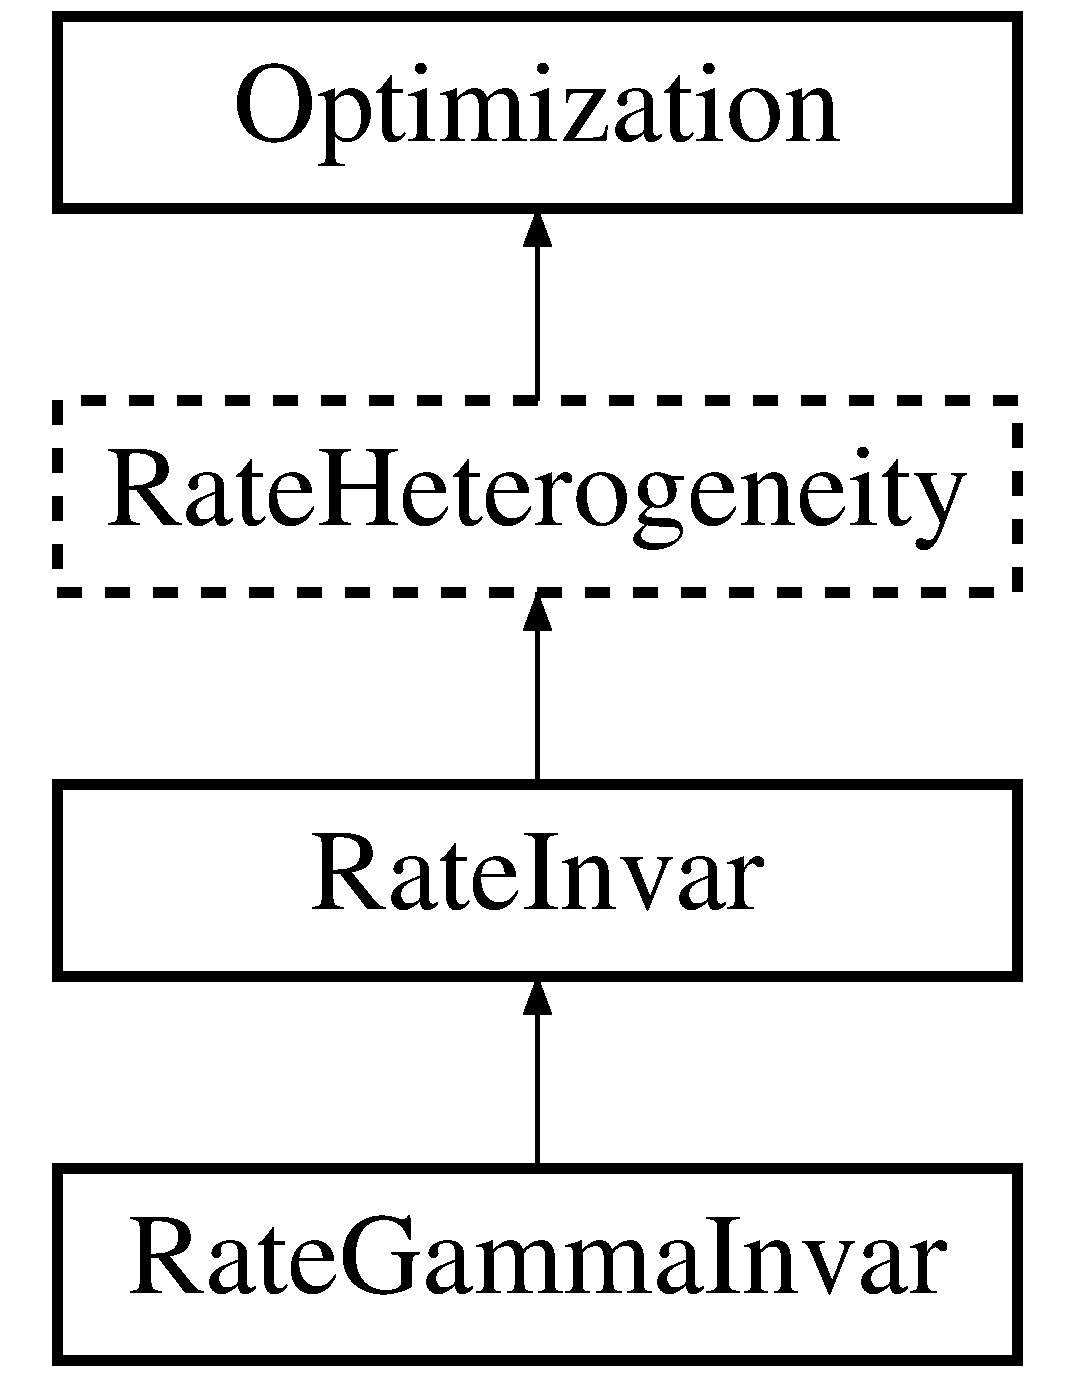
\includegraphics[height=4cm]{classRateInvar}
\end{center}
\end{figure}
\subsection*{Public Member Functions}
\begin{DoxyCompactItemize}
\item 
\hyperlink{classRateInvar_ae78abd45146e41b786f6e0a7b8bd5747}{RateInvar} (\hyperlink{classPhyloTree}{PhyloTree} $\ast$tree)
\item 
virtual double \hyperlink{classRateInvar_a750aa513c32453d28cc50b14bb31a9a7}{getPInvar} ()
\item 
virtual double \hyperlink{classRateInvar_a593bcac4c771b4b69c2f286ed8789793}{optimizeParameters} ()
\item 
virtual double \hyperlink{classRateInvar_a23d4b3aed6205e4f121a3aee43996a49}{computeFunction} (double p\_\-invar\_\-value)
\item 
virtual int \hyperlink{classRateInvar_a3ffa388d5aa7f56bb2c047c35bc3b453}{getNDim} ()
\item 
virtual void \hyperlink{classRateInvar_a6b8c198319557891db9b91fb47b27428}{writeInfo} (ostream \&out)
\item 
virtual void \hyperlink{classRateInvar_aabcef1cc18777b54b0f8644ccb00913c}{writeParameters} (ostream \&out)
\end{DoxyCompactItemize}
\subsection*{Public Attributes}
\begin{DoxyCompactItemize}
\item 
double \hyperlink{classRateInvar_af6b377196f15c6f58d115b8c24ddf00f}{p\_\-invar}
\end{DoxyCompactItemize}


\subsection{Detailed Description}
class for rate heterogeneity with a fraction of invariable sites

\begin{DoxyAuthor}{Author}
BUI Quang Minh $<$\href{mailto:minh.bui@univie.ac.at}{\tt minh.bui@univie.ac.at}$>$ 
\end{DoxyAuthor}


\subsection{Constructor \& Destructor Documentation}
\hypertarget{classRateInvar_ae78abd45146e41b786f6e0a7b8bd5747}{
\index{RateInvar@{RateInvar}!RateInvar@{RateInvar}}
\index{RateInvar@{RateInvar}!RateInvar@{RateInvar}}
\subsubsection[{RateInvar}]{\setlength{\rightskip}{0pt plus 5cm}RateInvar::RateInvar ({\bf PhyloTree} $\ast$ {\em tree})}}
\label{classRateInvar_ae78abd45146e41b786f6e0a7b8bd5747}
constructor 
\begin{DoxyParams}{Parameters}
\item[{\em tree}]associated phylogenetic tree \end{DoxyParams}


\subsection{Member Function Documentation}
\hypertarget{classRateInvar_a23d4b3aed6205e4f121a3aee43996a49}{
\index{RateInvar@{RateInvar}!computeFunction@{computeFunction}}
\index{computeFunction@{computeFunction}!RateInvar@{RateInvar}}
\subsubsection[{computeFunction}]{\setlength{\rightskip}{0pt plus 5cm}double RateInvar::computeFunction (double {\em p\_\-invar\_\-value})\hspace{0.3cm}{\ttfamily  \mbox{[}virtual\mbox{]}}}}
\label{classRateInvar_a23d4b3aed6205e4f121a3aee43996a49}
override function from \hyperlink{classOptimization}{Optimization} class, used by the \hyperlink{classOptimization_a59ccdfae81744716ce48226da029d470}{minimizeOneDimen()} to optimize p\_\-invar parameter 

Reimplemented from \hyperlink{classOptimization_ad7ca7b884076f8c76312d516e23c6609}{Optimization}.

Reimplemented in \hyperlink{classRateGammaInvar_a48fde92a023867c5d0656572f8dc0f71}{RateGammaInvar}.\hypertarget{classRateInvar_a3ffa388d5aa7f56bb2c047c35bc3b453}{
\index{RateInvar@{RateInvar}!getNDim@{getNDim}}
\index{getNDim@{getNDim}!RateInvar@{RateInvar}}
\subsubsection[{getNDim}]{\setlength{\rightskip}{0pt plus 5cm}virtual int RateInvar::getNDim ()\hspace{0.3cm}{\ttfamily  \mbox{[}inline, virtual\mbox{]}}}}
\label{classRateInvar_a3ffa388d5aa7f56bb2c047c35bc3b453}
return the number of dimensions 

Reimplemented from \hyperlink{classOptimization_a6d04cefb0969f3cac9b607aa1412eb57}{Optimization}.

Reimplemented in \hyperlink{classRateGammaInvar_a4f276d1639a79eece217b365439049c7}{RateGammaInvar}.\hypertarget{classRateInvar_a750aa513c32453d28cc50b14bb31a9a7}{
\index{RateInvar@{RateInvar}!getPInvar@{getPInvar}}
\index{getPInvar@{getPInvar}!RateInvar@{RateInvar}}
\subsubsection[{getPInvar}]{\setlength{\rightskip}{0pt plus 5cm}virtual double RateInvar::getPInvar ()\hspace{0.3cm}{\ttfamily  \mbox{[}inline, virtual\mbox{]}}}}
\label{classRateInvar_a750aa513c32453d28cc50b14bb31a9a7}
get the proportion of invariable sites \begin{DoxyReturn}{Returns}
the proportion of invariable sites 
\end{DoxyReturn}


Reimplemented from \hyperlink{classRateHeterogeneity_ada76d84ed7f66ddde02734d9c72f4e7b}{RateHeterogeneity}.\hypertarget{classRateInvar_a593bcac4c771b4b69c2f286ed8789793}{
\index{RateInvar@{RateInvar}!optimizeParameters@{optimizeParameters}}
\index{optimizeParameters@{optimizeParameters}!RateInvar@{RateInvar}}
\subsubsection[{optimizeParameters}]{\setlength{\rightskip}{0pt plus 5cm}double RateInvar::optimizeParameters ()\hspace{0.3cm}{\ttfamily  \mbox{[}virtual\mbox{]}}}}
\label{classRateInvar_a593bcac4c771b4b69c2f286ed8789793}
optimize parameters \begin{DoxyReturn}{Returns}
the best likelihood 
\end{DoxyReturn}


Reimplemented from \hyperlink{classRateHeterogeneity_a1305d5b8481dd5a2482917ddb5fe57bd}{RateHeterogeneity}.

Reimplemented in \hyperlink{classRateGammaInvar_ab72a2559cea978d312a243d521c2abef}{RateGammaInvar}.\hypertarget{classRateInvar_a6b8c198319557891db9b91fb47b27428}{
\index{RateInvar@{RateInvar}!writeInfo@{writeInfo}}
\index{writeInfo@{writeInfo}!RateInvar@{RateInvar}}
\subsubsection[{writeInfo}]{\setlength{\rightskip}{0pt plus 5cm}void RateInvar::writeInfo (ostream \& {\em out})\hspace{0.3cm}{\ttfamily  \mbox{[}virtual\mbox{]}}}}
\label{classRateInvar_a6b8c198319557891db9b91fb47b27428}
write information 
\begin{DoxyParams}{Parameters}
\item[{\em out}]output stream \end{DoxyParams}


Reimplemented from \hyperlink{classRateHeterogeneity_a520772859d465036b6620bdbf2977efe}{RateHeterogeneity}.

Reimplemented in \hyperlink{classRateGammaInvar_a428c3ac79ba1bf28da546f602d4b0f7b}{RateGammaInvar}.\hypertarget{classRateInvar_aabcef1cc18777b54b0f8644ccb00913c}{
\index{RateInvar@{RateInvar}!writeParameters@{writeParameters}}
\index{writeParameters@{writeParameters}!RateInvar@{RateInvar}}
\subsubsection[{writeParameters}]{\setlength{\rightskip}{0pt plus 5cm}void RateInvar::writeParameters (ostream \& {\em out})\hspace{0.3cm}{\ttfamily  \mbox{[}virtual\mbox{]}}}}
\label{classRateInvar_aabcef1cc18777b54b0f8644ccb00913c}
write parameters, used with modeltest 
\begin{DoxyParams}{Parameters}
\item[{\em out}]output stream \end{DoxyParams}


Reimplemented from \hyperlink{classRateHeterogeneity_ad2832e686971cf1f2cac2a6f842a3550}{RateHeterogeneity}.

Reimplemented in \hyperlink{classRateGammaInvar_a13b6629de9e3579aacff555f1bd76db5}{RateGammaInvar}.

\subsection{Member Data Documentation}
\hypertarget{classRateInvar_af6b377196f15c6f58d115b8c24ddf00f}{
\index{RateInvar@{RateInvar}!p\_\-invar@{p\_\-invar}}
\index{p\_\-invar@{p\_\-invar}!RateInvar@{RateInvar}}
\subsubsection[{p\_\-invar}]{\setlength{\rightskip}{0pt plus 5cm}double {\bf RateInvar::p\_\-invar}}}
\label{classRateInvar_af6b377196f15c6f58d115b8c24ddf00f}
proportion of invariable sites 

The documentation for this class was generated from the following files:\begin{DoxyCompactItemize}
\item 
src/rateinvar.h\item 
src/rateinvar.cpp\end{DoxyCompactItemize}

\hypertarget{classSplit}{
\section{Split Class Reference}
\label{classSplit}\index{Split@{Split}}
}


{\ttfamily \#include $<$split.h$>$}\subsection*{Public Member Functions}
\begin{DoxyCompactItemize}
\item 
\hyperlink{classSplit_a365a552fc4d3a0599c50ef629a691be4}{Split} ()
\item 
\hyperlink{classSplit_a94a33c0e8cfb74c40df1839c1a0bd843}{Split} (int antaxa, double aweight=0.0)
\item 
\hyperlink{classSplit_ad98691b8ee7de01dc6bb66eb5937f0ce}{Split} (const \hyperlink{classSplit}{Split} \&sp)
\item 
\hyperlink{classSplit_a9ef1d15c79111653ea9f2af81327630a}{Split} (int antaxa, double aweight, vector$<$ int $>$ taxa\_\-list)
\item 
void \hyperlink{classSplit_a62f6f9dd6849b2e3b5f4ff8d1a3131fd}{report} (ostream \&out)
\item 
\hyperlink{classSplit_a32ae47628734299802a079d19b70fc0a}{$\sim$Split} ()
\item 
int \hyperlink{classSplit_a3a2fd4ded9bc1d43c5cdb69b3d057e71}{getNTaxa} () const 
\item 
int \hyperlink{classSplit_af7441915bc8fed4333541b193e0394f4}{countTaxa} () const 
\item 
void \hyperlink{classSplit_a2d5be14eadb830619216ef12ddd512e7}{setNTaxa} (int antaxa)
\item 
int \hyperlink{classSplit_a2d63d14c00fa83c87afca7a412bced5d}{firstTaxon} ()
\item 
bool \hyperlink{classSplit_abb9262185c7f5bf5b9f6604c432a796f}{isEmpty} ()
\item 
double \hyperlink{classSplit_a08d9beb4e3b391de5b2aa13c57ea99ca}{getWeight} () const 
\item 
void \hyperlink{classSplit_a4c2f157bcf99e1522415915bb6823bb9}{setWeight} (double aweight)
\item 
bool \hyperlink{classSplit_a1e801d80a5667c140ee3f1ebe0137f07}{shouldInvert} ()
\item 
void \hyperlink{classSplit_aa1c5426a32b64ee0e56e980096a0074c}{invert} ()
\item 
bool \hyperlink{classSplit_afbf535c1d11bf7651ecd733045f2d688}{compatible} (\hyperlink{classSplit}{Split} \&sp)
\item 
bool \hyperlink{classSplit_a164299ace7e47de37ebe8f9daeda8fc8}{preserved} (\hyperlink{classSplit}{Split} \&taxa\_\-set)
\item 
int \hyperlink{classSplit_a96875580ea7a3e02f013951ba4b41596}{trivial} ()
\item 
void \hyperlink{classSplit_a35b159b165b623a7ee1d33bab6a1368f}{addTaxon} (int tax\_\-id)
\item 
void \hyperlink{classSplit_a35df7b8abdab57e1a8a097909a125396}{removeTaxon} (int tax\_\-id)
\item 
bool \hyperlink{classSplit_a080cf81fd05ba6487dfd9130b8b9787b}{containTaxon} (int tax\_\-id)
\item 
bool \hyperlink{classSplit_afffa3f41c2edcf5c66e8875a8151941d}{containAny} (IntVector \&tax\_\-id)
\item 
bool \hyperlink{classSplit_aaac9e8b488cf55b0d92bee3687abf40e}{containAll} (IntVector \&tax\_\-id)
\item 
void \hyperlink{classSplit_a6432380add76d5dd97ed106e2d6d10e6}{getTaxaList} (vector$<$ int $>$ \&invec)
\item 
void \hyperlink{classSplit_ab8f398ac2532dbeb5697cb2fc4e5ce6b}{getTaxaList} (vector$<$ int $>$ \&invec, vector$<$ int $>$ \&outvec)
\item 
bool \hyperlink{classSplit_ad74cb390339b148f3bc45e3e4db8ac58}{operator==} (const \hyperlink{classSplit}{Split} \&sp) const 
\item 
\hyperlink{classSplit}{Split} \& \hyperlink{classSplit_a553102b9ea76d19445a4071b822d17b0}{operator+=} (\hyperlink{classSplit}{Split} \&sp)
\item 
\hyperlink{classSplit}{Split} \& \hyperlink{classSplit_ac9be6ec283224b571f14353f348b251e}{operator$\ast$=} (\hyperlink{classSplit}{Split} \&sp)
\item 
\hyperlink{classSplit}{Split} \& \hyperlink{classSplit_a510547abdad1acc043c104810a936fa8}{operator-\/=} (\hyperlink{classSplit}{Split} \&sp)
\item 
bool \hyperlink{classSplit_a50109c1755bdaa7143295515bcd5be44}{overlap} (\hyperlink{classSplit}{Split} \&sp)
\item 
\hyperlink{classSplit}{Split} \& \hyperlink{classSplit_ab8d66a1714b54f7e1a1a0c714b2e1175}{operator=} (const \hyperlink{classSplit}{Split} \&sp)
\item 
bool \hyperlink{classSplit_a724c4b8226835191fb058048f5a5aff3}{subsetOf} (\hyperlink{classSplit}{Split} \&sp)
\item 
void \hyperlink{classSplit_aba2bc06ac8b0864cd7210e181de41275}{randomize} (int size)
\end{DoxyCompactItemize}
\subsection*{Protected Attributes}
\begin{DoxyCompactItemize}
\item 
int \hyperlink{classSplit_a41a18ab8832241bb319a4ddbca3af8b5}{ntaxa}
\item 
double \hyperlink{classSplit_aa8845f08e5d041e68ed0475fca6954c5}{weight}
\end{DoxyCompactItemize}
\subsection*{Friends}
\begin{DoxyCompactItemize}
\item 
\hypertarget{classSplit_ad180a9052e2cfb059a0ea9d7b370ec7b}{
class \hyperlink{classSplit_ad180a9052e2cfb059a0ea9d7b370ec7b}{MSplitsBlock}}
\label{classSplit_ad180a9052e2cfb059a0ea9d7b370ec7b}

\item 
\hypertarget{classSplit_ab8ea3e9164803ba3b6b59fab949bd0f3}{
class \hyperlink{classSplit_ab8ea3e9164803ba3b6b59fab949bd0f3}{SplitGraph}}
\label{classSplit_ab8ea3e9164803ba3b6b59fab949bd0f3}

\item 
\hypertarget{classSplit_aa341ce7452c8af86ea325aa7eff2f02d}{
class \hyperlink{classSplit_aa341ce7452c8af86ea325aa7eff2f02d}{PDNetwork}}
\label{classSplit_aa341ce7452c8af86ea325aa7eff2f02d}

\item 
\hypertarget{classSplit_a1615e6a0c22088bac5824899e6c3fa6e}{
class \hyperlink{classSplit_a1615e6a0c22088bac5824899e6c3fa6e}{CircularNetwork}}
\label{classSplit_a1615e6a0c22088bac5824899e6c3fa6e}

\item 
\hypertarget{classSplit_a5ea42f356770ae950d06d0e4917f93ad}{
class \hyperlink{classSplit_a5ea42f356770ae950d06d0e4917f93ad}{PDTree}}
\label{classSplit_a5ea42f356770ae950d06d0e4917f93ad}

\end{DoxyCompactItemize}


\subsection{Detailed Description}
Defining a split, also a set of taxa.

\begin{DoxyAuthor}{Author}
BUI Quang Minh, Steffen Klaere, Arndt von Haeseler 
\end{DoxyAuthor}


\subsection{Constructor \& Destructor Documentation}
\hypertarget{classSplit_a365a552fc4d3a0599c50ef629a691be4}{
\index{Split@{Split}!Split@{Split}}
\index{Split@{Split}!Split@{Split}}
\subsubsection[{Split}]{\setlength{\rightskip}{0pt plus 5cm}Split::Split ()}}
\label{classSplit_a365a552fc4d3a0599c50ef629a691be4}
empty constructor \hypertarget{classSplit_a94a33c0e8cfb74c40df1839c1a0bd843}{
\index{Split@{Split}!Split@{Split}}
\index{Split@{Split}!Split@{Split}}
\subsubsection[{Split}]{\setlength{\rightskip}{0pt plus 5cm}Split::Split (int {\em antaxa}, \/  double {\em aweight} = {\ttfamily 0.0})}}
\label{classSplit_a94a33c0e8cfb74c40df1839c1a0bd843}
constructor 
\begin{DoxyParams}{Parameters}
\item[{\em antaxa}]number of taxa \item[{\em aweight}]weight of split \end{DoxyParams}
\hypertarget{classSplit_ad98691b8ee7de01dc6bb66eb5937f0ce}{
\index{Split@{Split}!Split@{Split}}
\index{Split@{Split}!Split@{Split}}
\subsubsection[{Split}]{\setlength{\rightskip}{0pt plus 5cm}Split::Split (const {\bf Split} \& {\em sp})}}
\label{classSplit_ad98691b8ee7de01dc6bb66eb5937f0ce}
constructor copy from another split 
\begin{DoxyParams}{Parameters}
\item[{\em sp}]split to be copied from \end{DoxyParams}
\hypertarget{classSplit_a9ef1d15c79111653ea9f2af81327630a}{
\index{Split@{Split}!Split@{Split}}
\index{Split@{Split}!Split@{Split}}
\subsubsection[{Split}]{\setlength{\rightskip}{0pt plus 5cm}Split::Split (int {\em antaxa}, \/  double {\em aweight}, \/  vector$<$ int $>$ {\em taxa\_\-list})}}
\label{classSplit_a9ef1d15c79111653ea9f2af81327630a}
construct the split from a taxa list 
\begin{DoxyParams}{Parameters}
\item[{\em antaxa}]number of taxa \item[{\em aweight}]weight of split \item[{\em taxa\_\-list}]list of taxa in one side of split \end{DoxyParams}
\hypertarget{classSplit_a32ae47628734299802a079d19b70fc0a}{
\index{Split@{Split}!$\sim$Split@{$\sim$Split}}
\index{$\sim$Split@{$\sim$Split}!Split@{Split}}
\subsubsection[{$\sim$Split}]{\setlength{\rightskip}{0pt plus 5cm}Split::$\sim$Split ()}}
\label{classSplit_a32ae47628734299802a079d19b70fc0a}
destructor 

\subsection{Member Function Documentation}
\hypertarget{classSplit_a35b159b165b623a7ee1d33bab6a1368f}{
\index{Split@{Split}!addTaxon@{addTaxon}}
\index{addTaxon@{addTaxon}!Split@{Split}}
\subsubsection[{addTaxon}]{\setlength{\rightskip}{0pt plus 5cm}void Split::addTaxon (int {\em tax\_\-id})}}
\label{classSplit_a35b159b165b623a7ee1d33bab6a1368f}
add a taxon into the split 
\begin{DoxyParams}{Parameters}
\item[{\em tax\_\-id}]id of taxon from 0..ntaxa-\/1 \end{DoxyParams}
\hypertarget{classSplit_afbf535c1d11bf7651ecd733045f2d688}{
\index{Split@{Split}!compatible@{compatible}}
\index{compatible@{compatible}!Split@{Split}}
\subsubsection[{compatible}]{\setlength{\rightskip}{0pt plus 5cm}bool Split::compatible ({\bf Split} \& {\em sp})}}
\label{classSplit_afbf535c1d11bf7651ecd733045f2d688}

\begin{DoxyParams}{Parameters}
\item[{\em sp}]the other split \end{DoxyParams}
\begin{DoxyReturn}{Returns}
true if this split is compatible with sp 
\end{DoxyReturn}
\hypertarget{classSplit_aaac9e8b488cf55b0d92bee3687abf40e}{
\index{Split@{Split}!containAll@{containAll}}
\index{containAll@{containAll}!Split@{Split}}
\subsubsection[{containAll}]{\setlength{\rightskip}{0pt plus 5cm}bool Split::containAll (IntVector \& {\em tax\_\-id})}}
\label{classSplit_aaac9e8b488cf55b0d92bee3687abf40e}

\begin{DoxyParams}{Parameters}
\item[{\em tax\_\-id}]vector of id of taxa from 0..ntaxa-\/1 \end{DoxyParams}
\begin{DoxyReturn}{Returns}
true if ALL taxa in tax\_\-id is in the set 
\end{DoxyReturn}
\hypertarget{classSplit_afffa3f41c2edcf5c66e8875a8151941d}{
\index{Split@{Split}!containAny@{containAny}}
\index{containAny@{containAny}!Split@{Split}}
\subsubsection[{containAny}]{\setlength{\rightskip}{0pt plus 5cm}bool Split::containAny (IntVector \& {\em tax\_\-id})}}
\label{classSplit_afffa3f41c2edcf5c66e8875a8151941d}

\begin{DoxyParams}{Parameters}
\item[{\em tax\_\-id}]vector of id of taxa from 0..ntaxa-\/1 \end{DoxyParams}
\begin{DoxyReturn}{Returns}
true if SOME taxon in tax\_\-id is in the set 
\end{DoxyReturn}
\hypertarget{classSplit_a080cf81fd05ba6487dfd9130b8b9787b}{
\index{Split@{Split}!containTaxon@{containTaxon}}
\index{containTaxon@{containTaxon}!Split@{Split}}
\subsubsection[{containTaxon}]{\setlength{\rightskip}{0pt plus 5cm}bool Split::containTaxon (int {\em tax\_\-id})}}
\label{classSplit_a080cf81fd05ba6487dfd9130b8b9787b}

\begin{DoxyParams}{Parameters}
\item[{\em tax\_\-id}]id of taxon from 0..ntaxa-\/1 \end{DoxyParams}
\begin{DoxyReturn}{Returns}
true if tax\_\-id is in the set 
\end{DoxyReturn}
\hypertarget{classSplit_af7441915bc8fed4333541b193e0394f4}{
\index{Split@{Split}!countTaxa@{countTaxa}}
\index{countTaxa@{countTaxa}!Split@{Split}}
\subsubsection[{countTaxa}]{\setlength{\rightskip}{0pt plus 5cm}int Split::countTaxa () const}}
\label{classSplit_af7441915bc8fed4333541b193e0394f4}
get number of taxa being in the split \begin{DoxyReturn}{Returns}
number of taxa 
\end{DoxyReturn}
\hypertarget{classSplit_a2d63d14c00fa83c87afca7a412bced5d}{
\index{Split@{Split}!firstTaxon@{firstTaxon}}
\index{firstTaxon@{firstTaxon}!Split@{Split}}
\subsubsection[{firstTaxon}]{\setlength{\rightskip}{0pt plus 5cm}int Split::firstTaxon ()}}
\label{classSplit_a2d63d14c00fa83c87afca7a412bced5d}
get the first taxon in the set \begin{DoxyReturn}{Returns}
the first taxon or -\/1 if empty 
\end{DoxyReturn}
\hypertarget{classSplit_a3a2fd4ded9bc1d43c5cdb69b3d057e71}{
\index{Split@{Split}!getNTaxa@{getNTaxa}}
\index{getNTaxa@{getNTaxa}!Split@{Split}}
\subsubsection[{getNTaxa}]{\setlength{\rightskip}{0pt plus 5cm}int Split::getNTaxa () const\hspace{0.3cm}{\ttfamily  \mbox{[}inline\mbox{]}}}}
\label{classSplit_a3a2fd4ded9bc1d43c5cdb69b3d057e71}
get number of taxa \begin{DoxyReturn}{Returns}
number of taxa 
\end{DoxyReturn}
\hypertarget{classSplit_ab8f398ac2532dbeb5697cb2fc4e5ce6b}{
\index{Split@{Split}!getTaxaList@{getTaxaList}}
\index{getTaxaList@{getTaxaList}!Split@{Split}}
\subsubsection[{getTaxaList}]{\setlength{\rightskip}{0pt plus 5cm}void Split::getTaxaList (vector$<$ int $>$ \& {\em invec}, \/  vector$<$ int $>$ \& {\em outvec})}}
\label{classSplit_ab8f398ac2532dbeb5697cb2fc4e5ce6b}
get the list of taxa contained in split and not contained in split 
\begin{DoxyParams}{Parameters}
\item[{\em invec}](OUT) taxa in this side of split \item[{\em outvec}](OUT) taxa on the other side \end{DoxyParams}
\hypertarget{classSplit_a6432380add76d5dd97ed106e2d6d10e6}{
\index{Split@{Split}!getTaxaList@{getTaxaList}}
\index{getTaxaList@{getTaxaList}!Split@{Split}}
\subsubsection[{getTaxaList}]{\setlength{\rightskip}{0pt plus 5cm}void Split::getTaxaList (vector$<$ int $>$ \& {\em invec})}}
\label{classSplit_a6432380add76d5dd97ed106e2d6d10e6}
get the list of taxa contained in split 
\begin{DoxyParams}{Parameters}
\item[{\em invec}](OUT) taxa in this side of split \end{DoxyParams}
\hypertarget{classSplit_a08d9beb4e3b391de5b2aa13c57ea99ca}{
\index{Split@{Split}!getWeight@{getWeight}}
\index{getWeight@{getWeight}!Split@{Split}}
\subsubsection[{getWeight}]{\setlength{\rightskip}{0pt plus 5cm}double Split::getWeight () const\hspace{0.3cm}{\ttfamily  \mbox{[}inline\mbox{]}}}}
\label{classSplit_a08d9beb4e3b391de5b2aa13c57ea99ca}
get weight \begin{DoxyReturn}{Returns}
weight 
\end{DoxyReturn}
\hypertarget{classSplit_aa1c5426a32b64ee0e56e980096a0074c}{
\index{Split@{Split}!invert@{invert}}
\index{invert@{invert}!Split@{Split}}
\subsubsection[{invert}]{\setlength{\rightskip}{0pt plus 5cm}void Split::invert ()}}
\label{classSplit_aa1c5426a32b64ee0e56e980096a0074c}
invert the split (0-\/$>$1, 1-\/$>$0) \hypertarget{classSplit_abb9262185c7f5bf5b9f6604c432a796f}{
\index{Split@{Split}!isEmpty@{isEmpty}}
\index{isEmpty@{isEmpty}!Split@{Split}}
\subsubsection[{isEmpty}]{\setlength{\rightskip}{0pt plus 5cm}bool Split::isEmpty ()}}
\label{classSplit_abb9262185c7f5bf5b9f6604c432a796f}
\begin{DoxyReturn}{Returns}
TRUE if the set is empty 
\end{DoxyReturn}
\hypertarget{classSplit_ac9be6ec283224b571f14353f348b251e}{
\index{Split@{Split}!operator$\ast$=@{operator$\ast$=}}
\index{operator$\ast$=@{operator$\ast$=}!Split@{Split}}
\subsubsection[{operator$\ast$=}]{\setlength{\rightskip}{0pt plus 5cm}{\bf Split} \& Split::operator$\ast$= ({\bf Split} \& {\em sp})}}
\label{classSplit_ac9be6ec283224b571f14353f348b251e}
get the intersection with another split 
\begin{DoxyParams}{Parameters}
\item[{\em sp}]a split \end{DoxyParams}
\hypertarget{classSplit_a553102b9ea76d19445a4071b822d17b0}{
\index{Split@{Split}!operator+=@{operator+=}}
\index{operator+=@{operator+=}!Split@{Split}}
\subsubsection[{operator+=}]{\setlength{\rightskip}{0pt plus 5cm}{\bf Split} \& Split::operator+= ({\bf Split} \& {\em sp})}}
\label{classSplit_a553102b9ea76d19445a4071b822d17b0}
add all taxa from another split into this split (union) 
\begin{DoxyParams}{Parameters}
\item[{\em sp}]a split \end{DoxyParams}
\hypertarget{classSplit_a510547abdad1acc043c104810a936fa8}{
\index{Split@{Split}!operator-\/=@{operator-\/=}}
\index{operator-\/=@{operator-\/=}!Split@{Split}}
\subsubsection[{operator-\/=}]{\setlength{\rightskip}{0pt plus 5cm}{\bf Split} \& Split::operator-\/= ({\bf Split} \& {\em sp})}}
\label{classSplit_a510547abdad1acc043c104810a936fa8}
get the set difference with another split 
\begin{DoxyParams}{Parameters}
\item[{\em sp}]a split \end{DoxyParams}
\hypertarget{classSplit_ab8d66a1714b54f7e1a1a0c714b2e1175}{
\index{Split@{Split}!operator=@{operator=}}
\index{operator=@{operator=}!Split@{Split}}
\subsubsection[{operator=}]{\setlength{\rightskip}{0pt plus 5cm}{\bf Split} \& Split::operator= (const {\bf Split} \& {\em sp})}}
\label{classSplit_ab8d66a1714b54f7e1a1a0c714b2e1175}
assignment 
\begin{DoxyParams}{Parameters}
\item[{\em sp}]a split \end{DoxyParams}
\hypertarget{classSplit_ad74cb390339b148f3bc45e3e4db8ac58}{
\index{Split@{Split}!operator==@{operator==}}
\index{operator==@{operator==}!Split@{Split}}
\subsubsection[{operator==}]{\setlength{\rightskip}{0pt plus 5cm}bool Split::operator== (const {\bf Split} \& {\em sp}) const}}
\label{classSplit_ad74cb390339b148f3bc45e3e4db8ac58}
compare two split, do not compare the weight 
\begin{DoxyParams}{Parameters}
\item[{\em sp}]the target split \end{DoxyParams}
\begin{DoxyReturn}{Returns}
TRUE if equal, FALSE otherwise 
\end{DoxyReturn}
\hypertarget{classSplit_a50109c1755bdaa7143295515bcd5be44}{
\index{Split@{Split}!overlap@{overlap}}
\index{overlap@{overlap}!Split@{Split}}
\subsubsection[{overlap}]{\setlength{\rightskip}{0pt plus 5cm}bool Split::overlap ({\bf Split} \& {\em sp})}}
\label{classSplit_a50109c1755bdaa7143295515bcd5be44}
\begin{DoxyReturn}{Returns}
TRUE if there is overlapped taxon with sp, FALSE otherwise 
\end{DoxyReturn}

\begin{DoxyParams}{Parameters}
\item[{\em sp}]a split \end{DoxyParams}
\hypertarget{classSplit_a164299ace7e47de37ebe8f9daeda8fc8}{
\index{Split@{Split}!preserved@{preserved}}
\index{preserved@{preserved}!Split@{Split}}
\subsubsection[{preserved}]{\setlength{\rightskip}{0pt plus 5cm}bool Split::preserved ({\bf Split} \& {\em taxa\_\-set})}}
\label{classSplit_a164299ace7e47de37ebe8f9daeda8fc8}

\begin{DoxyParams}{Parameters}
\item[{\em taxa\_\-set}]set of taxa \end{DoxyParams}
\begin{DoxyReturn}{Returns}
true if this split is preserved in the set taxa\_\-set 
\end{DoxyReturn}
\hypertarget{classSplit_aba2bc06ac8b0864cd7210e181de41275}{
\index{Split@{Split}!randomize@{randomize}}
\index{randomize@{randomize}!Split@{Split}}
\subsubsection[{randomize}]{\setlength{\rightskip}{0pt plus 5cm}void Split::randomize (int {\em size})}}
\label{classSplit_aba2bc06ac8b0864cd7210e181de41275}
randomize the set of a specific size 
\begin{DoxyParams}{Parameters}
\item[{\em size}]number of taxa in the resulting set \end{DoxyParams}
\hypertarget{classSplit_a35df7b8abdab57e1a8a097909a125396}{
\index{Split@{Split}!removeTaxon@{removeTaxon}}
\index{removeTaxon@{removeTaxon}!Split@{Split}}
\subsubsection[{removeTaxon}]{\setlength{\rightskip}{0pt plus 5cm}void Split::removeTaxon (int {\em tax\_\-id})}}
\label{classSplit_a35df7b8abdab57e1a8a097909a125396}
remove a taxon from the split 
\begin{DoxyParams}{Parameters}
\item[{\em tax\_\-id}]id of taxon from 0..ntaxa-\/1 \end{DoxyParams}
\hypertarget{classSplit_a62f6f9dd6849b2e3b5f4ff8d1a3131fd}{
\index{Split@{Split}!report@{report}}
\index{report@{report}!Split@{Split}}
\subsubsection[{report}]{\setlength{\rightskip}{0pt plus 5cm}void Split::report (ostream \& {\em out})}}
\label{classSplit_a62f6f9dd6849b2e3b5f4ff8d1a3131fd}
print infos of split graph 
\begin{DoxyParams}{Parameters}
\item[{\em out}]the output stream \end{DoxyParams}
\hypertarget{classSplit_a2d5be14eadb830619216ef12ddd512e7}{
\index{Split@{Split}!setNTaxa@{setNTaxa}}
\index{setNTaxa@{setNTaxa}!Split@{Split}}
\subsubsection[{setNTaxa}]{\setlength{\rightskip}{0pt plus 5cm}void Split::setNTaxa (int {\em antaxa})}}
\label{classSplit_a2d5be14eadb830619216ef12ddd512e7}
copy from another split set number of taxa 
\begin{DoxyParams}{Parameters}
\item[{\em antaxa}]number of taxa\end{DoxyParams}
set number of taxa 
\begin{DoxyParams}{Parameters}
\item[{\em antaxa}]number of taxa \end{DoxyParams}
\hypertarget{classSplit_a4c2f157bcf99e1522415915bb6823bb9}{
\index{Split@{Split}!setWeight@{setWeight}}
\index{setWeight@{setWeight}!Split@{Split}}
\subsubsection[{setWeight}]{\setlength{\rightskip}{0pt plus 5cm}void Split::setWeight (double {\em aweight})\hspace{0.3cm}{\ttfamily  \mbox{[}inline\mbox{]}}}}
\label{classSplit_a4c2f157bcf99e1522415915bb6823bb9}
set weight 
\begin{DoxyParams}{Parameters}
\item[{\em aweight}]the new weight \end{DoxyParams}
\hypertarget{classSplit_a1e801d80a5667c140ee3f1ebe0137f07}{
\index{Split@{Split}!shouldInvert@{shouldInvert}}
\index{shouldInvert@{shouldInvert}!Split@{Split}}
\subsubsection[{shouldInvert}]{\setlength{\rightskip}{0pt plus 5cm}bool Split::shouldInvert ()}}
\label{classSplit_a1e801d80a5667c140ee3f1ebe0137f07}
check whether the split should be inverted (number of taxa $>$ ntaxa / 2) \begin{DoxyReturn}{Returns}
TRUE yes, should be inverted 
\end{DoxyReturn}
\hypertarget{classSplit_a724c4b8226835191fb058048f5a5aff3}{
\index{Split@{Split}!subsetOf@{subsetOf}}
\index{subsetOf@{subsetOf}!Split@{Split}}
\subsubsection[{subsetOf}]{\setlength{\rightskip}{0pt plus 5cm}bool Split::subsetOf ({\bf Split} \& {\em sp})}}
\label{classSplit_a724c4b8226835191fb058048f5a5aff3}
subset operator 
\begin{DoxyParams}{Parameters}
\item[{\em sp}]a split \end{DoxyParams}
\begin{DoxyReturn}{Returns}
TRUE of this set is a subset of sp 
\end{DoxyReturn}
\hypertarget{classSplit_a96875580ea7a3e02f013951ba4b41596}{
\index{Split@{Split}!trivial@{trivial}}
\index{trivial@{trivial}!Split@{Split}}
\subsubsection[{trivial}]{\setlength{\rightskip}{0pt plus 5cm}int Split::trivial ()}}
\label{classSplit_a96875580ea7a3e02f013951ba4b41596}
if the split is trivial (contains 1 taxon in 1 side), return the taxon id, otherwise return -\/1 \begin{DoxyReturn}{Returns}
the taxon id if the split is trivial 
\end{DoxyReturn}


\subsection{Member Data Documentation}
\hypertarget{classSplit_a41a18ab8832241bb319a4ddbca3af8b5}{
\index{Split@{Split}!ntaxa@{ntaxa}}
\index{ntaxa@{ntaxa}!Split@{Split}}
\subsubsection[{ntaxa}]{\setlength{\rightskip}{0pt plus 5cm}int {\bf Split::ntaxa}\hspace{0.3cm}{\ttfamily  \mbox{[}protected\mbox{]}}}}
\label{classSplit_a41a18ab8832241bb319a4ddbca3af8b5}
number of taxa \hypertarget{classSplit_aa8845f08e5d041e68ed0475fca6954c5}{
\index{Split@{Split}!weight@{weight}}
\index{weight@{weight}!Split@{Split}}
\subsubsection[{weight}]{\setlength{\rightskip}{0pt plus 5cm}double {\bf Split::weight}\hspace{0.3cm}{\ttfamily  \mbox{[}protected\mbox{]}}}}
\label{classSplit_aa8845f08e5d041e68ed0475fca6954c5}
weight of split 

The documentation for this class was generated from the following files:\begin{DoxyCompactItemize}
\item 
src/split.h\item 
src/split.cpp\end{DoxyCompactItemize}

\hypertarget{classSplitGraph}{
\section{SplitGraph Class Reference}
\label{classSplitGraph}\index{SplitGraph@{SplitGraph}}
}


{\ttfamily \#include $<$splitgraph.h$>$}Inheritance diagram for SplitGraph::\begin{figure}[H]
\begin{center}
\leavevmode
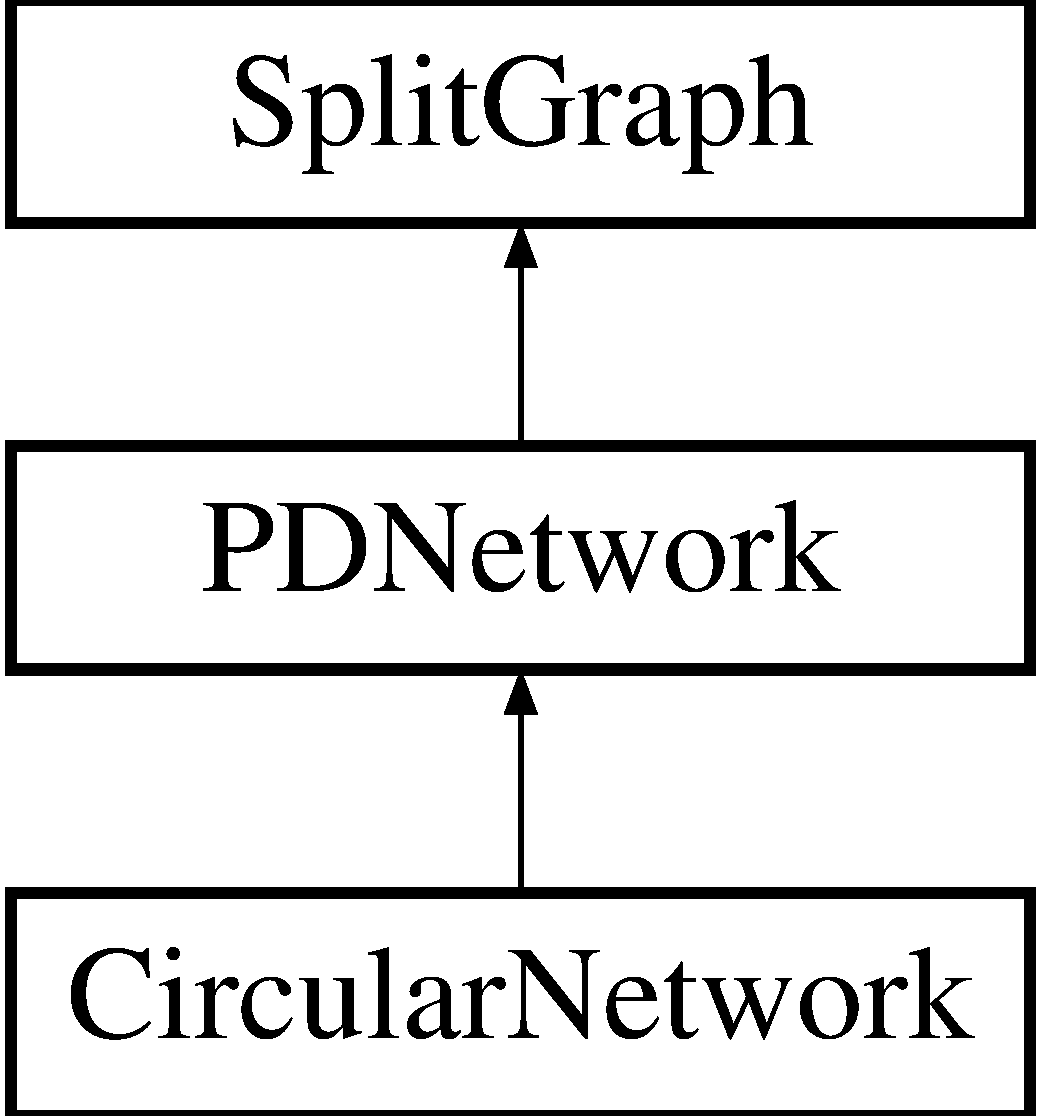
\includegraphics[height=3cm]{classSplitGraph}
\end{center}
\end{figure}
\subsection*{Public Member Functions}
\begin{DoxyCompactItemize}
\item 
\hyperlink{classSplitGraph_aea160f196766a6573809410979e0df5b}{SplitGraph} ()
\item 
\hyperlink{classSplitGraph_aec55fe3e947b56545f57c9c596ec20a3}{SplitGraph} (\hyperlink{structParams}{Params} \&params)
\item 
void \hyperlink{classSplitGraph_a0111a637ecb711d90f2f15ce734a96c8}{init} (\hyperlink{structParams}{Params} \&params)
\item 
void \hyperlink{classSplitGraph_adb64089273f29e935d82a5fc74289792}{AddTaxaFromSets} ()
\item 
void \hyperlink{classSplitGraph_af306b9e7b96b0fc89d664548e2b6769a}{createStarTree} ()
\item 
void \hyperlink{classSplitGraph_a05d34dc9d03a3aed2e195b64acd698b0}{createBlocks} ()
\item 
virtual \hyperlink{classSplitGraph_a40780d552131a67c8cdb5b20037dbd16}{$\sim$SplitGraph} ()
\item 
void \hyperlink{classSplitGraph_a9cc756e24638ce4b7f78605c8ccb6543}{convertFromTreesBlock} (int burnin, double split\_\-threshold)
\item 
void \hyperlink{classSplitGraph_abd01f1db37dbb2c97becef1b38032dd9}{report} (ostream \&out)
\item 
void \hyperlink{classSplitGraph_a1876d549d833982752e4ad2e263ec6d4}{reportConflict} (ostream \&out)
\item 
double \hyperlink{classSplitGraph_aaff18dd254098b4e1912593f0e2de524}{calcWeight} ()
\item 
double \hyperlink{classSplitGraph_a8ef03a25d1057fb09e2da7d9b3a28035}{calcTrivialWeight} ()
\item 
double \hyperlink{classSplitGraph_a9404a37b5c287146c432b7ca28c0ed6e}{calcWeight} (\hyperlink{classSplit}{Split} \&taxa\_\-set)
\item 
int \hyperlink{classSplitGraph_a9e3db1bb803fc6ee62082eae9978057d}{countSplits} (\hyperlink{classSplit}{Split} \&taxa\_\-set)
\item 
int \hyperlink{classSplitGraph_a8124b259486ab72f1a53119b11001805}{countInternalSplits} (\hyperlink{classSplit}{Split} \&taxa\_\-set)
\item 
void \hyperlink{classSplitGraph_aee545f263532bb4d56109fa43455a50a}{generateTaxaSet} (char $\ast$filename, int size, int overlap, int times)
\item 
void \hyperlink{classSplitGraph_aaa150a66ac97d6170336a9c74ffecc88}{scaleWeight} (double norm, bool make\_\-int=false)
\item 
bool \hyperlink{classSplitGraph_a43b37646702074556d3c7c894dbee9ca}{containSplit} (\hyperlink{classSplit}{Split} \&sp)
\item 
void \hyperlink{classSplitGraph_a870e02f7034993ce445ab9ae1964a781}{findMaxCompatibleSplits} (\hyperlink{classSplitGraph}{SplitGraph} \&maxsg)
\item 
bool \hyperlink{classSplitGraph_acaa3948107ecf6717cd11cd57829587e}{compatible} (\hyperlink{classSplit}{Split} $\ast$sp)
\item 
int \hyperlink{classSplitGraph_a779ae52f511731d598f6133ecb0deb51}{getNTaxa} ()
\item 
int \hyperlink{classSplitGraph_adfdcee57a677ea807d595328abb28481}{getNAreas} ()
\item 
int \hyperlink{classSplitGraph_a848a5f43fcb791dd99a1865d5fe9df46}{getNSplits} ()
\item 
int \hyperlink{classSplitGraph_a4e3c9a6363de8ac9d1bd15797306aaf1}{getNTrivialSplits} ()
\item 
\hyperlink{classNxsTaxaBlock}{NxsTaxaBlock} $\ast$ \hyperlink{classSplitGraph_a3f0181782d3b80190ea24a8eeb44b289}{getTaxa} ()
\item 
\hyperlink{classMSplitsBlock}{MSplitsBlock} $\ast$ \hyperlink{classSplitGraph_a4a4029deff1beb7089b3559790da4b2d}{getSplitsBlock} ()
\item 
\hyperlink{classMPdaBlock}{MPdaBlock} $\ast$ \hyperlink{classSplitGraph_a6eb74cff199a65a2e3b3a17c7a7c96e9}{getPdaBlock} ()
\item 
\hyperlink{classMSetsBlock}{MSetsBlock} $\ast$ \hyperlink{classSplitGraph_acafe07757402de0ed22320bcc2429f55}{getSetsBlock} ()
\item 
\hyperlink{classNxsTreesBlock}{NxsTreesBlock} $\ast$ \hyperlink{classSplitGraph_ad10d2632515ccf7b795cb9ace660e050}{getTreesBlock} ()
\item 
bool \hyperlink{classSplitGraph_ae7b98f722c61033d05cee4b1e2c68e54}{isCircular} ()
\item 
bool \hyperlink{classSplitGraph_a05cfb8141526a6cbc5905eb74dccc0fa}{isWeaklyCompatible} ()
\item 
bool \hyperlink{classSplitGraph_a93a2b7ec12a3f75f143a2dfada8d7a02}{isBudgetConstraint} ()
\item 
bool \hyperlink{classSplitGraph_aab13a9043727eb04c7afa61ddf489b8f}{checkCircular} (matrix(double)\&mat)
\item 
int \hyperlink{classSplitGraph_a3c7c98462a61153525cb22439f6872ff}{getCircleId} (int i)
\item 
void \hyperlink{classSplitGraph_a49e61357ca80dc01cc75891c1316a921}{generateCircular} (\hyperlink{structParams}{Params} \&params)
\item 
void \hyperlink{classSplitGraph_ac00dacfe044abd770bb24b5714035742}{saveFile} (ostream \&out)
\item 
void \hyperlink{classSplitGraph_aff71095a191dc17326d6da9441496c37}{calcDistance} (char $\ast$filename)
\item 
void \hyperlink{classSplitGraph_a1cbeb318350af0d36f70b03ae11bd46d}{calcDistance} (matrix(double)\&dist)
\item 
void \hyperlink{classSplitGraph_a9e96c1c785114aa2fc0c998702345228}{calcDistance} (matrix(double)\&dist, vector$<$ int $>$ \&taxa\_\-order)
\end{DoxyCompactItemize}
\subsection*{Protected Attributes}
\begin{DoxyCompactItemize}
\item 
\hyperlink{classNxsTaxaBlock}{NxsTaxaBlock} $\ast$ \hyperlink{classSplitGraph_a3166d128ac9e267baf86d309deadb988}{taxa}
\item 
\hyperlink{classMSplitsBlock}{MSplitsBlock} $\ast$ \hyperlink{classSplitGraph_a42f7001d83a322db0b47a4bab44eeebd}{splits}
\item 
\hyperlink{classMPdaBlock}{MPdaBlock} $\ast$ \hyperlink{classSplitGraph_ab5bb72994879bbc43abf1b48f1278c21}{pda}
\item 
\hyperlink{classMSetsBlock}{MSetsBlock} $\ast$ \hyperlink{classSplitGraph_ac46902cb0a5a2c914c657f0434d004bd}{sets}
\item 
\hyperlink{classNxsTreesBlock}{NxsTreesBlock} $\ast$ \hyperlink{classSplitGraph_ad3f25cc271cafddeb348ba92cbcb9f59}{trees}
\end{DoxyCompactItemize}
\subsection*{Friends}
\begin{DoxyCompactItemize}
\item 
\hypertarget{classSplitGraph_a7a747beac427dfc013c53501e474d452}{
class \hyperlink{classSplitGraph_a7a747beac427dfc013c53501e474d452}{MTree}}
\label{classSplitGraph_a7a747beac427dfc013c53501e474d452}

\item 
\hypertarget{classSplitGraph_a0f5ece1842cb079997e8b0826d310fcd}{
class \hyperlink{classSplitGraph_a0f5ece1842cb079997e8b0826d310fcd}{MTreeSet}}
\label{classSplitGraph_a0f5ece1842cb079997e8b0826d310fcd}

\end{DoxyCompactItemize}


\subsection{Detailed Description}
\hyperlink{classSplitGraph}{SplitGraph} class

\begin{DoxyAuthor}{Author}
BUI Quang Minh, Steffen Klaere, Arndt von Haeseler 
\end{DoxyAuthor}


\subsection{Constructor \& Destructor Documentation}
\hypertarget{classSplitGraph_aea160f196766a6573809410979e0df5b}{
\index{SplitGraph@{SplitGraph}!SplitGraph@{SplitGraph}}
\index{SplitGraph@{SplitGraph}!SplitGraph@{SplitGraph}}
\subsubsection[{SplitGraph}]{\setlength{\rightskip}{0pt plus 5cm}SplitGraph::SplitGraph ()}}
\label{classSplitGraph_aea160f196766a6573809410979e0df5b}
empty constructor \hypertarget{classSplitGraph_aec55fe3e947b56545f57c9c596ec20a3}{
\index{SplitGraph@{SplitGraph}!SplitGraph@{SplitGraph}}
\index{SplitGraph@{SplitGraph}!SplitGraph@{SplitGraph}}
\subsubsection[{SplitGraph}]{\setlength{\rightskip}{0pt plus 5cm}SplitGraph::SplitGraph ({\bf Params} \& {\em params})}}
\label{classSplitGraph_aec55fe3e947b56545f57c9c596ec20a3}
construct split graph from the parameters by calling init(params). 
\begin{DoxyParams}{Parameters}
\item[{\em params}]program parameters \end{DoxyParams}
\hypertarget{classSplitGraph_a40780d552131a67c8cdb5b20037dbd16}{
\index{SplitGraph@{SplitGraph}!$\sim$SplitGraph@{$\sim$SplitGraph}}
\index{$\sim$SplitGraph@{$\sim$SplitGraph}!SplitGraph@{SplitGraph}}
\subsubsection[{$\sim$SplitGraph}]{\setlength{\rightskip}{0pt plus 5cm}SplitGraph::$\sim$SplitGraph ()\hspace{0.3cm}{\ttfamily  \mbox{[}virtual\mbox{]}}}}
\label{classSplitGraph_a40780d552131a67c8cdb5b20037dbd16}
destructor 

\subsection{Member Function Documentation}
\hypertarget{classSplitGraph_adb64089273f29e935d82a5fc74289792}{
\index{SplitGraph@{SplitGraph}!AddTaxaFromSets@{AddTaxaFromSets}}
\index{AddTaxaFromSets@{AddTaxaFromSets}!SplitGraph@{SplitGraph}}
\subsubsection[{AddTaxaFromSets}]{\setlength{\rightskip}{0pt plus 5cm}void SplitGraph::AddTaxaFromSets ()}}
\label{classSplitGraph_adb64089273f29e935d82a5fc74289792}
if no taxa block found, but the sets block is present, then this function will be invoked. It takes the taxa names from the sets block. \hypertarget{classSplitGraph_a9e96c1c785114aa2fc0c998702345228}{
\index{SplitGraph@{SplitGraph}!calcDistance@{calcDistance}}
\index{calcDistance@{calcDistance}!SplitGraph@{SplitGraph}}
\subsubsection[{calcDistance}]{\setlength{\rightskip}{0pt plus 5cm}void SplitGraph::calcDistance (matrix(double)\& {\em dist}, \/  vector$<$ int $>$ \& {\em taxa\_\-order})}}
\label{classSplitGraph_a9e96c1c785114aa2fc0c998702345228}
calculate the distance matrix, based on the taxa\_\-order 
\begin{DoxyParams}{Parameters}
\item[{\em dist}](OUT) distance matrix \item[{\em taxa\_\-order}]an order of taxa \end{DoxyParams}
\hypertarget{classSplitGraph_a1cbeb318350af0d36f70b03ae11bd46d}{
\index{SplitGraph@{SplitGraph}!calcDistance@{calcDistance}}
\index{calcDistance@{calcDistance}!SplitGraph@{SplitGraph}}
\subsubsection[{calcDistance}]{\setlength{\rightskip}{0pt plus 5cm}void SplitGraph::calcDistance (matrix(double)\& {\em dist})}}
\label{classSplitGraph_a1cbeb318350af0d36f70b03ae11bd46d}
calculate the distance matrix 
\begin{DoxyParams}{Parameters}
\item[{\em dist}](OUT) distance matrix \end{DoxyParams}
\hypertarget{classSplitGraph_aff71095a191dc17326d6da9441496c37}{
\index{SplitGraph@{SplitGraph}!calcDistance@{calcDistance}}
\index{calcDistance@{calcDistance}!SplitGraph@{SplitGraph}}
\subsubsection[{calcDistance}]{\setlength{\rightskip}{0pt plus 5cm}void SplitGraph::calcDistance (char $\ast$ {\em filename})}}
\label{classSplitGraph_aff71095a191dc17326d6da9441496c37}
calculate the distance matrix, print to file in phylip format 
\begin{DoxyParams}{Parameters}
\item[{\em filename}]output file name \end{DoxyParams}
\hypertarget{classSplitGraph_a8ef03a25d1057fb09e2da7d9b3a28035}{
\index{SplitGraph@{SplitGraph}!calcTrivialWeight@{calcTrivialWeight}}
\index{calcTrivialWeight@{calcTrivialWeight}!SplitGraph@{SplitGraph}}
\subsubsection[{calcTrivialWeight}]{\setlength{\rightskip}{0pt plus 5cm}double SplitGraph::calcTrivialWeight ()}}
\label{classSplitGraph_a8ef03a25d1057fb09e2da7d9b3a28035}
calculate sum of weights of all trivial splits \hypertarget{classSplitGraph_a9404a37b5c287146c432b7ca28c0ed6e}{
\index{SplitGraph@{SplitGraph}!calcWeight@{calcWeight}}
\index{calcWeight@{calcWeight}!SplitGraph@{SplitGraph}}
\subsubsection[{calcWeight}]{\setlength{\rightskip}{0pt plus 5cm}double SplitGraph::calcWeight ({\bf Split} \& {\em taxa\_\-set})}}
\label{classSplitGraph_a9404a37b5c287146c432b7ca28c0ed6e}
calculate sum of weights of preserved splits in the taxa\_\-set 
\begin{DoxyParams}{Parameters}
\item[{\em taxa\_\-set}]a set of taxa \end{DoxyParams}
\hypertarget{classSplitGraph_aaff18dd254098b4e1912593f0e2de524}{
\index{SplitGraph@{SplitGraph}!calcWeight@{calcWeight}}
\index{calcWeight@{calcWeight}!SplitGraph@{SplitGraph}}
\subsubsection[{calcWeight}]{\setlength{\rightskip}{0pt plus 5cm}double SplitGraph::calcWeight ()}}
\label{classSplitGraph_aaff18dd254098b4e1912593f0e2de524}
calculate sum of weights of all splits \hypertarget{classSplitGraph_aab13a9043727eb04c7afa61ddf489b8f}{
\index{SplitGraph@{SplitGraph}!checkCircular@{checkCircular}}
\index{checkCircular@{checkCircular}!SplitGraph@{SplitGraph}}
\subsubsection[{checkCircular}]{\setlength{\rightskip}{0pt plus 5cm}bool SplitGraph::checkCircular (matrix(double)\& {\em mat})}}
\label{classSplitGraph_aab13a9043727eb04c7afa61ddf489b8f}
\begin{DoxyReturn}{Returns}
TRUE if the distance matrix presents for circular splits graph 
\end{DoxyReturn}

\begin{DoxyParams}{Parameters}
\item[{\em mat}]distance matrix \end{DoxyParams}
\hypertarget{classSplitGraph_acaa3948107ecf6717cd11cd57829587e}{
\index{SplitGraph@{SplitGraph}!compatible@{compatible}}
\index{compatible@{compatible}!SplitGraph@{SplitGraph}}
\subsubsection[{compatible}]{\setlength{\rightskip}{0pt plus 5cm}bool SplitGraph::compatible ({\bf Split} $\ast$ {\em sp})}}
\label{classSplitGraph_acaa3948107ecf6717cd11cd57829587e}
check the compatibility of sp against all splits in this set 
\begin{DoxyParams}{Parameters}
\item[{\em sp}]the target split \end{DoxyParams}
\begin{DoxyReturn}{Returns}
TRUE if sp is compatible with all splits here, otherwise FALSE 
\end{DoxyReturn}
\hypertarget{classSplitGraph_a43b37646702074556d3c7c894dbee9ca}{
\index{SplitGraph@{SplitGraph}!containSplit@{containSplit}}
\index{containSplit@{containSplit}!SplitGraph@{SplitGraph}}
\subsubsection[{containSplit}]{\setlength{\rightskip}{0pt plus 5cm}bool SplitGraph::containSplit ({\bf Split} \& {\em sp})}}
\label{classSplitGraph_a43b37646702074556d3c7c894dbee9ca}
\begin{DoxyReturn}{Returns}
TRUE if split sp is contained in the split system 
\end{DoxyReturn}

\begin{DoxyParams}{Parameters}
\item[{\em sp}]target split to search for \end{DoxyParams}
\hypertarget{classSplitGraph_a9cc756e24638ce4b7f78605c8ccb6543}{
\index{SplitGraph@{SplitGraph}!convertFromTreesBlock@{convertFromTreesBlock}}
\index{convertFromTreesBlock@{convertFromTreesBlock}!SplitGraph@{SplitGraph}}
\subsubsection[{convertFromTreesBlock}]{\setlength{\rightskip}{0pt plus 5cm}void SplitGraph::convertFromTreesBlock (int {\em burnin}, \/  double {\em split\_\-threshold})}}
\label{classSplitGraph_a9cc756e24638ce4b7f78605c8ccb6543}
convert the collection of trees in TREES block into this split graph 
\begin{DoxyParams}{Parameters}
\item[{\em burnin}]the number of beginning trees to be discarded \item[{\em split\_\-threshold}]only keep those splits which appear more than this threshold \end{DoxyParams}
\hypertarget{classSplitGraph_a8124b259486ab72f1a53119b11001805}{
\index{SplitGraph@{SplitGraph}!countInternalSplits@{countInternalSplits}}
\index{countInternalSplits@{countInternalSplits}!SplitGraph@{SplitGraph}}
\subsubsection[{countInternalSplits}]{\setlength{\rightskip}{0pt plus 5cm}int SplitGraph::countInternalSplits ({\bf Split} \& {\em taxa\_\-set})}}
\label{classSplitGraph_a8124b259486ab72f1a53119b11001805}
count how many internal splits are covered by the taxon set 
\begin{DoxyParams}{Parameters}
\item[{\em taxa\_\-set}]a set of taxa \end{DoxyParams}
\hypertarget{classSplitGraph_a9e3db1bb803fc6ee62082eae9978057d}{
\index{SplitGraph@{SplitGraph}!countSplits@{countSplits}}
\index{countSplits@{countSplits}!SplitGraph@{SplitGraph}}
\subsubsection[{countSplits}]{\setlength{\rightskip}{0pt plus 5cm}int SplitGraph::countSplits ({\bf Split} \& {\em taxa\_\-set})}}
\label{classSplitGraph_a9e3db1bb803fc6ee62082eae9978057d}
count how many splits are covered by the taxon set 
\begin{DoxyParams}{Parameters}
\item[{\em taxa\_\-set}]a set of taxa \end{DoxyParams}
\hypertarget{classSplitGraph_a05d34dc9d03a3aed2e195b64acd698b0}{
\index{SplitGraph@{SplitGraph}!createBlocks@{createBlocks}}
\index{createBlocks@{createBlocks}!SplitGraph@{SplitGraph}}
\subsubsection[{createBlocks}]{\setlength{\rightskip}{0pt plus 5cm}void SplitGraph::createBlocks ()}}
\label{classSplitGraph_a05d34dc9d03a3aed2e195b64acd698b0}
new all blocks: taxa, splits, pda \hypertarget{classSplitGraph_af306b9e7b96b0fc89d664548e2b6769a}{
\index{SplitGraph@{SplitGraph}!createStarTree@{createStarTree}}
\index{createStarTree@{createStarTree}!SplitGraph@{SplitGraph}}
\subsubsection[{createStarTree}]{\setlength{\rightskip}{0pt plus 5cm}void SplitGraph::createStarTree ()}}
\label{classSplitGraph_af306b9e7b96b0fc89d664548e2b6769a}
this function is invoked \hypertarget{classSplitGraph_a870e02f7034993ce445ab9ae1964a781}{
\index{SplitGraph@{SplitGraph}!findMaxCompatibleSplits@{findMaxCompatibleSplits}}
\index{findMaxCompatibleSplits@{findMaxCompatibleSplits}!SplitGraph@{SplitGraph}}
\subsubsection[{findMaxCompatibleSplits}]{\setlength{\rightskip}{0pt plus 5cm}void SplitGraph::findMaxCompatibleSplits ({\bf SplitGraph} \& {\em maxsg})}}
\label{classSplitGraph_a870e02f7034993ce445ab9ae1964a781}
find the maximum-\/weight set of compatible splits 
\begin{DoxyParams}{Parameters}
\item[{\em maxsg}](OUT) set of compatible splits in a split graph class \end{DoxyParams}
\hypertarget{classSplitGraph_a49e61357ca80dc01cc75891c1316a921}{
\index{SplitGraph@{SplitGraph}!generateCircular@{generateCircular}}
\index{generateCircular@{generateCircular}!SplitGraph@{SplitGraph}}
\subsubsection[{generateCircular}]{\setlength{\rightskip}{0pt plus 5cm}void SplitGraph::generateCircular ({\bf Params} \& {\em params})}}
\label{classSplitGraph_a49e61357ca80dc01cc75891c1316a921}
generate a random circular split graph 
\begin{DoxyParams}{Parameters}
\item[{\em params}]program parameters \end{DoxyParams}
\hypertarget{classSplitGraph_aee545f263532bb4d56109fa43455a50a}{
\index{SplitGraph@{SplitGraph}!generateTaxaSet@{generateTaxaSet}}
\index{generateTaxaSet@{generateTaxaSet}!SplitGraph@{SplitGraph}}
\subsubsection[{generateTaxaSet}]{\setlength{\rightskip}{0pt plus 5cm}void SplitGraph::generateTaxaSet (char $\ast$ {\em filename}, \/  int {\em size}, \/  int {\em overlap}, \/  int {\em times})}}
\label{classSplitGraph_aee545f263532bb4d56109fa43455a50a}
generate pairs of random taxa set with overlap of taxa in common 
\begin{DoxyParams}{Parameters}
\item[{\em filename}]output file name \item[{\em size}]size of the taxa set \item[{\em overlap}]number of taxa common in both sets \item[{\em times}]number of times repeated \end{DoxyParams}
\hypertarget{classSplitGraph_a3c7c98462a61153525cb22439f6872ff}{
\index{SplitGraph@{SplitGraph}!getCircleId@{getCircleId}}
\index{getCircleId@{getCircleId}!SplitGraph@{SplitGraph}}
\subsubsection[{getCircleId}]{\setlength{\rightskip}{0pt plus 5cm}int SplitGraph::getCircleId (int {\em i})\hspace{0.3cm}{\ttfamily  \mbox{[}inline\mbox{]}}}}
\label{classSplitGraph_a3c7c98462a61153525cb22439f6872ff}
get the ID of the taxon around the circle in a circular splits graph 
\begin{DoxyParams}{Parameters}
\item[{\em i}]a taxon \end{DoxyParams}
\begin{DoxyReturn}{Returns}
index of taxon on the circle 
\end{DoxyReturn}
\hypertarget{classSplitGraph_adfdcee57a677ea807d595328abb28481}{
\index{SplitGraph@{SplitGraph}!getNAreas@{getNAreas}}
\index{getNAreas@{getNAreas}!SplitGraph@{SplitGraph}}
\subsubsection[{getNAreas}]{\setlength{\rightskip}{0pt plus 5cm}int SplitGraph::getNAreas ()\hspace{0.3cm}{\ttfamily  \mbox{[}inline\mbox{]}}}}
\label{classSplitGraph_adfdcee57a677ea807d595328abb28481}
\begin{DoxyReturn}{Returns}
number of areas 
\end{DoxyReturn}
\hypertarget{classSplitGraph_a848a5f43fcb791dd99a1865d5fe9df46}{
\index{SplitGraph@{SplitGraph}!getNSplits@{getNSplits}}
\index{getNSplits@{getNSplits}!SplitGraph@{SplitGraph}}
\subsubsection[{getNSplits}]{\setlength{\rightskip}{0pt plus 5cm}int SplitGraph::getNSplits ()\hspace{0.3cm}{\ttfamily  \mbox{[}inline\mbox{]}}}}
\label{classSplitGraph_a848a5f43fcb791dd99a1865d5fe9df46}
\begin{DoxyReturn}{Returns}
number of splits 
\end{DoxyReturn}
\hypertarget{classSplitGraph_a779ae52f511731d598f6133ecb0deb51}{
\index{SplitGraph@{SplitGraph}!getNTaxa@{getNTaxa}}
\index{getNTaxa@{getNTaxa}!SplitGraph@{SplitGraph}}
\subsubsection[{getNTaxa}]{\setlength{\rightskip}{0pt plus 5cm}int SplitGraph::getNTaxa ()\hspace{0.3cm}{\ttfamily  \mbox{[}inline\mbox{]}}}}
\label{classSplitGraph_a779ae52f511731d598f6133ecb0deb51}
\begin{DoxyReturn}{Returns}
number of taxa 
\end{DoxyReturn}
\hypertarget{classSplitGraph_a4e3c9a6363de8ac9d1bd15797306aaf1}{
\index{SplitGraph@{SplitGraph}!getNTrivialSplits@{getNTrivialSplits}}
\index{getNTrivialSplits@{getNTrivialSplits}!SplitGraph@{SplitGraph}}
\subsubsection[{getNTrivialSplits}]{\setlength{\rightskip}{0pt plus 5cm}int SplitGraph::getNTrivialSplits ()}}
\label{classSplitGraph_a4e3c9a6363de8ac9d1bd15797306aaf1}
\begin{DoxyReturn}{Returns}
number of trivial splits 
\end{DoxyReturn}
\hypertarget{classSplitGraph_a6eb74cff199a65a2e3b3a17c7a7c96e9}{
\index{SplitGraph@{SplitGraph}!getPdaBlock@{getPdaBlock}}
\index{getPdaBlock@{getPdaBlock}!SplitGraph@{SplitGraph}}
\subsubsection[{getPdaBlock}]{\setlength{\rightskip}{0pt plus 5cm}{\bf MPdaBlock}$\ast$ SplitGraph::getPdaBlock ()\hspace{0.3cm}{\ttfamily  \mbox{[}inline\mbox{]}}}}
\label{classSplitGraph_a6eb74cff199a65a2e3b3a17c7a7c96e9}
\begin{DoxyReturn}{Returns}
PDA block 
\end{DoxyReturn}
\hypertarget{classSplitGraph_acafe07757402de0ed22320bcc2429f55}{
\index{SplitGraph@{SplitGraph}!getSetsBlock@{getSetsBlock}}
\index{getSetsBlock@{getSetsBlock}!SplitGraph@{SplitGraph}}
\subsubsection[{getSetsBlock}]{\setlength{\rightskip}{0pt plus 5cm}{\bf MSetsBlock}$\ast$ SplitGraph::getSetsBlock ()\hspace{0.3cm}{\ttfamily  \mbox{[}inline\mbox{]}}}}
\label{classSplitGraph_acafe07757402de0ed22320bcc2429f55}
\begin{DoxyReturn}{Returns}
SETS block 
\end{DoxyReturn}
\hypertarget{classSplitGraph_a4a4029deff1beb7089b3559790da4b2d}{
\index{SplitGraph@{SplitGraph}!getSplitsBlock@{getSplitsBlock}}
\index{getSplitsBlock@{getSplitsBlock}!SplitGraph@{SplitGraph}}
\subsubsection[{getSplitsBlock}]{\setlength{\rightskip}{0pt plus 5cm}{\bf MSplitsBlock}$\ast$ SplitGraph::getSplitsBlock ()\hspace{0.3cm}{\ttfamily  \mbox{[}inline\mbox{]}}}}
\label{classSplitGraph_a4a4029deff1beb7089b3559790da4b2d}
\begin{DoxyReturn}{Returns}
splits block 
\end{DoxyReturn}
\hypertarget{classSplitGraph_a3f0181782d3b80190ea24a8eeb44b289}{
\index{SplitGraph@{SplitGraph}!getTaxa@{getTaxa}}
\index{getTaxa@{getTaxa}!SplitGraph@{SplitGraph}}
\subsubsection[{getTaxa}]{\setlength{\rightskip}{0pt plus 5cm}{\bf NxsTaxaBlock}$\ast$ SplitGraph::getTaxa ()\hspace{0.3cm}{\ttfamily  \mbox{[}inline\mbox{]}}}}
\label{classSplitGraph_a3f0181782d3b80190ea24a8eeb44b289}
\begin{DoxyReturn}{Returns}
taxa block 
\end{DoxyReturn}
\hypertarget{classSplitGraph_ad10d2632515ccf7b795cb9ace660e050}{
\index{SplitGraph@{SplitGraph}!getTreesBlock@{getTreesBlock}}
\index{getTreesBlock@{getTreesBlock}!SplitGraph@{SplitGraph}}
\subsubsection[{getTreesBlock}]{\setlength{\rightskip}{0pt plus 5cm}{\bf NxsTreesBlock}$\ast$ SplitGraph::getTreesBlock ()\hspace{0.3cm}{\ttfamily  \mbox{[}inline\mbox{]}}}}
\label{classSplitGraph_ad10d2632515ccf7b795cb9ace660e050}
\begin{DoxyReturn}{Returns}
TREES block 
\end{DoxyReturn}
\hypertarget{classSplitGraph_a0111a637ecb711d90f2f15ce734a96c8}{
\index{SplitGraph@{SplitGraph}!init@{init}}
\index{init@{init}!SplitGraph@{SplitGraph}}
\subsubsection[{init}]{\setlength{\rightskip}{0pt plus 5cm}void SplitGraph::init ({\bf Params} \& {\em params})}}
\label{classSplitGraph_a0111a637ecb711d90f2f15ce734a96c8}
init split graph from the parameters 
\begin{DoxyParams}{Parameters}
\item[{\em params}]program parameters \end{DoxyParams}
\hypertarget{classSplitGraph_a93a2b7ec12a3f75f143a2dfada8d7a02}{
\index{SplitGraph@{SplitGraph}!isBudgetConstraint@{isBudgetConstraint}}
\index{isBudgetConstraint@{isBudgetConstraint}!SplitGraph@{SplitGraph}}
\subsubsection[{isBudgetConstraint}]{\setlength{\rightskip}{0pt plus 5cm}bool SplitGraph::isBudgetConstraint ()\hspace{0.3cm}{\ttfamily  \mbox{[}inline\mbox{]}}}}
\label{classSplitGraph_a93a2b7ec12a3f75f143a2dfada8d7a02}
\begin{DoxyReturn}{Returns}
TRUE if it is the cost-\/constrained PD problem 
\end{DoxyReturn}
\hypertarget{classSplitGraph_ae7b98f722c61033d05cee4b1e2c68e54}{
\index{SplitGraph@{SplitGraph}!isCircular@{isCircular}}
\index{isCircular@{isCircular}!SplitGraph@{SplitGraph}}
\subsubsection[{isCircular}]{\setlength{\rightskip}{0pt plus 5cm}bool SplitGraph::isCircular ()\hspace{0.3cm}{\ttfamily  \mbox{[}inline\mbox{]}}}}
\label{classSplitGraph_ae7b98f722c61033d05cee4b1e2c68e54}
\begin{DoxyReturn}{Returns}
TRUE if splits graph is circular 
\end{DoxyReturn}
\hypertarget{classSplitGraph_a05cfb8141526a6cbc5905eb74dccc0fa}{
\index{SplitGraph@{SplitGraph}!isWeaklyCompatible@{isWeaklyCompatible}}
\index{isWeaklyCompatible@{isWeaklyCompatible}!SplitGraph@{SplitGraph}}
\subsubsection[{isWeaklyCompatible}]{\setlength{\rightskip}{0pt plus 5cm}bool SplitGraph::isWeaklyCompatible ()}}
\label{classSplitGraph_a05cfb8141526a6cbc5905eb74dccc0fa}
\begin{DoxyReturn}{Returns}
TRUE if split system is weakly compatible 
\end{DoxyReturn}
\hypertarget{classSplitGraph_abd01f1db37dbb2c97becef1b38032dd9}{
\index{SplitGraph@{SplitGraph}!report@{report}}
\index{report@{report}!SplitGraph@{SplitGraph}}
\subsubsection[{report}]{\setlength{\rightskip}{0pt plus 5cm}void SplitGraph::report (ostream \& {\em out})}}
\label{classSplitGraph_abd01f1db37dbb2c97becef1b38032dd9}
print infos of split graph 
\begin{DoxyParams}{Parameters}
\item[{\em out}]the output stream \end{DoxyParams}
\hypertarget{classSplitGraph_a1876d549d833982752e4ad2e263ec6d4}{
\index{SplitGraph@{SplitGraph}!reportConflict@{reportConflict}}
\index{reportConflict@{reportConflict}!SplitGraph@{SplitGraph}}
\subsubsection[{reportConflict}]{\setlength{\rightskip}{0pt plus 5cm}void SplitGraph::reportConflict (ostream \& {\em out})}}
\label{classSplitGraph_a1876d549d833982752e4ad2e263ec6d4}
print infos of compatibility graph of splits 
\begin{DoxyParams}{Parameters}
\item[{\em out}]the output stream \end{DoxyParams}
\hypertarget{classSplitGraph_ac00dacfe044abd770bb24b5714035742}{
\index{SplitGraph@{SplitGraph}!saveFile@{saveFile}}
\index{saveFile@{saveFile}!SplitGraph@{SplitGraph}}
\subsubsection[{saveFile}]{\setlength{\rightskip}{0pt plus 5cm}void SplitGraph::saveFile (ostream \& {\em out})}}
\label{classSplitGraph_ac00dacfe044abd770bb24b5714035742}
save split systems to a file 
\begin{DoxyParams}{Parameters}
\item[{\em out}]output stream \end{DoxyParams}
\hypertarget{classSplitGraph_aaa150a66ac97d6170336a9c74ffecc88}{
\index{SplitGraph@{SplitGraph}!scaleWeight@{scaleWeight}}
\index{scaleWeight@{scaleWeight}!SplitGraph@{SplitGraph}}
\subsubsection[{scaleWeight}]{\setlength{\rightskip}{0pt plus 5cm}void SplitGraph::scaleWeight (double {\em norm}, \/  bool {\em make\_\-int} = {\ttfamily false})}}
\label{classSplitGraph_aaa150a66ac97d6170336a9c74ffecc88}
scale the weight of all splits to a norm factor 
\begin{DoxyParams}{Parameters}
\item[{\em norm}]normalized factor \item[{\em make\_\-int}]TRUE to round weights to int, FALSE otherwise \end{DoxyParams}


\subsection{Member Data Documentation}
\hypertarget{classSplitGraph_ab5bb72994879bbc43abf1b48f1278c21}{
\index{SplitGraph@{SplitGraph}!pda@{pda}}
\index{pda@{pda}!SplitGraph@{SplitGraph}}
\subsubsection[{pda}]{\setlength{\rightskip}{0pt plus 5cm}{\bf MPdaBlock}$\ast$ {\bf SplitGraph::pda}\hspace{0.3cm}{\ttfamily  \mbox{[}protected\mbox{]}}}}
\label{classSplitGraph_ab5bb72994879bbc43abf1b48f1278c21}
PDA block \hypertarget{classSplitGraph_ac46902cb0a5a2c914c657f0434d004bd}{
\index{SplitGraph@{SplitGraph}!sets@{sets}}
\index{sets@{sets}!SplitGraph@{SplitGraph}}
\subsubsection[{sets}]{\setlength{\rightskip}{0pt plus 5cm}{\bf MSetsBlock}$\ast$ {\bf SplitGraph::sets}\hspace{0.3cm}{\ttfamily  \mbox{[}protected\mbox{]}}}}
\label{classSplitGraph_ac46902cb0a5a2c914c657f0434d004bd}
SETS block \hypertarget{classSplitGraph_a42f7001d83a322db0b47a4bab44eeebd}{
\index{SplitGraph@{SplitGraph}!splits@{splits}}
\index{splits@{splits}!SplitGraph@{SplitGraph}}
\subsubsection[{splits}]{\setlength{\rightskip}{0pt plus 5cm}{\bf MSplitsBlock}$\ast$ {\bf SplitGraph::splits}\hspace{0.3cm}{\ttfamily  \mbox{[}protected\mbox{]}}}}
\label{classSplitGraph_a42f7001d83a322db0b47a4bab44eeebd}
splits block \hypertarget{classSplitGraph_a3166d128ac9e267baf86d309deadb988}{
\index{SplitGraph@{SplitGraph}!taxa@{taxa}}
\index{taxa@{taxa}!SplitGraph@{SplitGraph}}
\subsubsection[{taxa}]{\setlength{\rightskip}{0pt plus 5cm}{\bf NxsTaxaBlock}$\ast$ {\bf SplitGraph::taxa}\hspace{0.3cm}{\ttfamily  \mbox{[}protected\mbox{]}}}}
\label{classSplitGraph_a3166d128ac9e267baf86d309deadb988}
taxa block \hypertarget{classSplitGraph_ad3f25cc271cafddeb348ba92cbcb9f59}{
\index{SplitGraph@{SplitGraph}!trees@{trees}}
\index{trees@{trees}!SplitGraph@{SplitGraph}}
\subsubsection[{trees}]{\setlength{\rightskip}{0pt plus 5cm}{\bf NxsTreesBlock}$\ast$ {\bf SplitGraph::trees}\hspace{0.3cm}{\ttfamily  \mbox{[}protected\mbox{]}}}}
\label{classSplitGraph_ad3f25cc271cafddeb348ba92cbcb9f59}
TREES block 

The documentation for this class was generated from the following files:\begin{DoxyCompactItemize}
\item 
src/splitgraph.h\item 
src/splitgraph.cpp\end{DoxyCompactItemize}

\hypertarget{classSplitIntMap}{
\section{SplitIntMap Class Reference}
\label{classSplitIntMap}\index{SplitIntMap@{SplitIntMap}}
}


{\ttfamily \#include $<$hashsplitset.h$>$}\subsection*{Public Member Functions}
\begin{DoxyCompactItemize}
\item 
\hyperlink{classSplit}{Split} $\ast$ \hyperlink{classSplitIntMap_ae86934b3eb2efeafda55f0e6a26bec09}{findSplit} (\hyperlink{classSplit}{Split} $\ast$sp)
\item 
\hyperlink{classSplit}{Split} $\ast$ \hyperlink{classSplitIntMap_abb18e331d550b889839b0f6427636512}{findSplit} (\hyperlink{classSplit}{Split} $\ast$sp, int \&value)
\item 
\hypertarget{classSplitIntMap_a922b1cf7f9415bea8a6d7b0b332cf7ab}{
int {\bfseries getValue} (\hyperlink{classSplit}{Split} $\ast$sp)}
\label{classSplitIntMap_a922b1cf7f9415bea8a6d7b0b332cf7ab}

\item 
\hypertarget{classSplitIntMap_a28c14844f8a7a6e381fe115ff49632db}{
void {\bfseries setValue} (\hyperlink{classSplit}{Split} $\ast$sp, int value)}
\label{classSplitIntMap_a28c14844f8a7a6e381fe115ff49632db}

\item 
\hypertarget{classSplitIntMap_aef719a7b617fc527072cc1579a3d6f2d}{
void {\bfseries eraseSplit} (\hyperlink{classSplit}{Split} $\ast$sp)}
\label{classSplitIntMap_aef719a7b617fc527072cc1579a3d6f2d}

\item 
\hypertarget{classSplitIntMap_acb0ff284023aa3b7dd3449a20f49c087}{
void {\bfseries insertSplit} (\hyperlink{classSplit}{Split} $\ast$sp, int value)}
\label{classSplitIntMap_acb0ff284023aa3b7dd3449a20f49c087}

\end{DoxyCompactItemize}


\subsection{Detailed Description}
\hyperlink{classSplitSet}{SplitSet} for quick search purpose

\begin{DoxyAuthor}{Author}
BUI Quang Minh, Steffen Klaere, Arndt von Haeseler 
\end{DoxyAuthor}


\subsection{Member Function Documentation}
\hypertarget{classSplitIntMap_abb18e331d550b889839b0f6427636512}{
\index{SplitIntMap@{SplitIntMap}!findSplit@{findSplit}}
\index{findSplit@{findSplit}!SplitIntMap@{SplitIntMap}}
\subsubsection[{findSplit}]{\setlength{\rightskip}{0pt plus 5cm}{\bf Split} $\ast$ SplitIntMap::findSplit ({\bf Split} $\ast$ {\em sp}, \/  int \& {\em value})}}
\label{classSplitIntMap_abb18e331d550b889839b0f6427636512}
find a split 
\begin{DoxyParams}{Parameters}
\item[{\em sp}]target split \item[{\em value}](OUT) associated value \end{DoxyParams}
\begin{DoxyReturn}{Returns}
the split containing the same set of taxa with sp, NULL if not found 
\end{DoxyReturn}
\hypertarget{classSplitIntMap_ae86934b3eb2efeafda55f0e6a26bec09}{
\index{SplitIntMap@{SplitIntMap}!findSplit@{findSplit}}
\index{findSplit@{findSplit}!SplitIntMap@{SplitIntMap}}
\subsubsection[{findSplit}]{\setlength{\rightskip}{0pt plus 5cm}{\bf Split} $\ast$ SplitIntMap::findSplit ({\bf Split} $\ast$ {\em sp})}}
\label{classSplitIntMap_ae86934b3eb2efeafda55f0e6a26bec09}
find a split 
\begin{DoxyParams}{Parameters}
\item[{\em sp}]target split \end{DoxyParams}
\begin{DoxyReturn}{Returns}
the split containing the same set of taxa with sp, NULL if not found 
\end{DoxyReturn}


The documentation for this class was generated from the following files:\begin{DoxyCompactItemize}
\item 
src/hashsplitset.h\item 
src/hashsplitset.cpp\end{DoxyCompactItemize}

\hypertarget{classSplitSet}{
\section{SplitSet Class Reference}
\label{classSplitSet}\index{SplitSet@{SplitSet}}
}


{\ttfamily \#include $<$splitset.h$>$}\subsection*{Public Member Functions}
\begin{DoxyCompactItemize}
\item 
void \hyperlink{classSplitSet_a6d18de51f6ef06b6f507f911a07468dc}{removeAll} ()
\item 
double \hyperlink{classSplitSet_ac1eced61b59973480c01fec6ad6ee7b5}{getWeight} ()
\item 
bool \hyperlink{classSplitSet_a4f71eb2dc2d5fd83a17680a539c0afe6}{compatible} (\hyperlink{classSplit}{Split} $\ast$sp)
\end{DoxyCompactItemize}


\subsection{Detailed Description}
Vector of Splits

\begin{DoxyAuthor}{Author}
BUI Quang Minh, Steffen Klaere, Arndt von Haeseler 
\end{DoxyAuthor}


\subsection{Member Function Documentation}
\hypertarget{classSplitSet_a4f71eb2dc2d5fd83a17680a539c0afe6}{
\index{SplitSet@{SplitSet}!compatible@{compatible}}
\index{compatible@{compatible}!SplitSet@{SplitSet}}
\subsubsection[{compatible}]{\setlength{\rightskip}{0pt plus 5cm}bool SplitSet::compatible ({\bf Split} $\ast$ {\em sp})}}
\label{classSplitSet_a4f71eb2dc2d5fd83a17680a539c0afe6}
check the compatibility of sp against all splits in this set 
\begin{DoxyParams}{Parameters}
\item[{\em sp}]the target split \end{DoxyParams}
\begin{DoxyReturn}{Returns}
TRUE if sp is compatible with all splits here, otherwise FALSE 
\end{DoxyReturn}
\hypertarget{classSplitSet_ac1eced61b59973480c01fec6ad6ee7b5}{
\index{SplitSet@{SplitSet}!getWeight@{getWeight}}
\index{getWeight@{getWeight}!SplitSet@{SplitSet}}
\subsubsection[{getWeight}]{\setlength{\rightskip}{0pt plus 5cm}double SplitSet::getWeight ()}}
\label{classSplitSet_ac1eced61b59973480c01fec6ad6ee7b5}
get the weight of the first split in the vector \hypertarget{classSplitSet_a6d18de51f6ef06b6f507f911a07468dc}{
\index{SplitSet@{SplitSet}!removeAll@{removeAll}}
\index{removeAll@{removeAll}!SplitSet@{SplitSet}}
\subsubsection[{removeAll}]{\setlength{\rightskip}{0pt plus 5cm}void SplitSet::removeAll ()}}
\label{classSplitSet_a6d18de51f6ef06b6f507f911a07468dc}
release the memory of all element splits, then resize to 0 

The documentation for this class was generated from the following files:\begin{DoxyCompactItemize}
\item 
src/splitset.h\item 
src/splitset.cpp\end{DoxyCompactItemize}

\hypertarget{structSPR__compare}{
\section{SPR\_\-compare Struct Reference}
\label{structSPR__compare}\index{SPR\_\-compare@{SPR\_\-compare}}
}
\subsection*{Public Member Functions}
\begin{DoxyCompactItemize}
\item 
\hypertarget{structSPR__compare_a791560826623de2e1d44f40d50d358df}{
bool {\bfseries operator()} (\hyperlink{structSPRMove}{SPRMove} s1, \hyperlink{structSPRMove}{SPRMove} s2) const }
\label{structSPR__compare_a791560826623de2e1d44f40d50d358df}

\end{DoxyCompactItemize}


The documentation for this struct was generated from the following file:\begin{DoxyCompactItemize}
\item 
src/phylotree.h\end{DoxyCompactItemize}

\hypertarget{structSPRMove}{
\section{SPRMove Struct Reference}
\label{structSPRMove}\index{SPRMove@{SPRMove}}
}


{\ttfamily \#include $<$phylotree.h$>$}\subsection*{Public Attributes}
\begin{DoxyCompactItemize}
\item 
\hypertarget{structSPRMove_af376cb761f6ce516ed57e85e09fbbade}{
\hyperlink{classPhyloNode}{PhyloNode} $\ast$ {\bfseries prune\_\-dad}}
\label{structSPRMove_af376cb761f6ce516ed57e85e09fbbade}

\item 
\hypertarget{structSPRMove_ac984f5c782a61af1e776a5f468676248}{
\hyperlink{classPhyloNode}{PhyloNode} $\ast$ {\bfseries prune\_\-node}}
\label{structSPRMove_ac984f5c782a61af1e776a5f468676248}

\item 
\hypertarget{structSPRMove_ae662434f95ac35c25962321f5d4a9dc0}{
\hyperlink{classPhyloNode}{PhyloNode} $\ast$ {\bfseries regraft\_\-dad}}
\label{structSPRMove_ae662434f95ac35c25962321f5d4a9dc0}

\item 
\hypertarget{structSPRMove_a5ddd25a002ae15e3894d379349546e8e}{
\hyperlink{classPhyloNode}{PhyloNode} $\ast$ {\bfseries regraft\_\-node}}
\label{structSPRMove_a5ddd25a002ae15e3894d379349546e8e}

\item 
\hypertarget{structSPRMove_aba800bc1903d31eb0594abfcaa2df4e3}{
double {\bfseries score}}
\label{structSPRMove_aba800bc1903d31eb0594abfcaa2df4e3}

\end{DoxyCompactItemize}


\subsection{Detailed Description}
an SPR move. 

The documentation for this struct was generated from the following file:\begin{DoxyCompactItemize}
\item 
src/phylotree.h\end{DoxyCompactItemize}

\hypertarget{classSPRMoves}{
\section{SPRMoves Class Reference}
\label{classSPRMoves}\index{SPRMoves@{SPRMoves}}
}
\subsection*{Public Member Functions}
\begin{DoxyCompactItemize}
\item 
\hypertarget{classSPRMoves_a93955f968fb9d282961e412a7d8d327c}{
void {\bfseries add} (\hyperlink{classPhyloNode}{PhyloNode} $\ast$prune\_\-node, \hyperlink{classPhyloNode}{PhyloNode} $\ast$prune\_\-dad, \hyperlink{classPhyloNode}{PhyloNode} $\ast$regraft\_\-node, \hyperlink{classPhyloNode}{PhyloNode} $\ast$regraft\_\-dad, double score)}
\label{classSPRMoves_a93955f968fb9d282961e412a7d8d327c}

\end{DoxyCompactItemize}


The documentation for this class was generated from the following files:\begin{DoxyCompactItemize}
\item 
src/phylotree.h\item 
src/phylotree.cpp\end{DoxyCompactItemize}

\hypertarget{classSubstModel}{
\section{SubstModel Class Reference}
\label{classSubstModel}\index{SubstModel@{SubstModel}}
}


{\ttfamily \#include $<$substmodel.h$>$}Inheritance diagram for SubstModel::\begin{figure}[H]
\begin{center}
\leavevmode
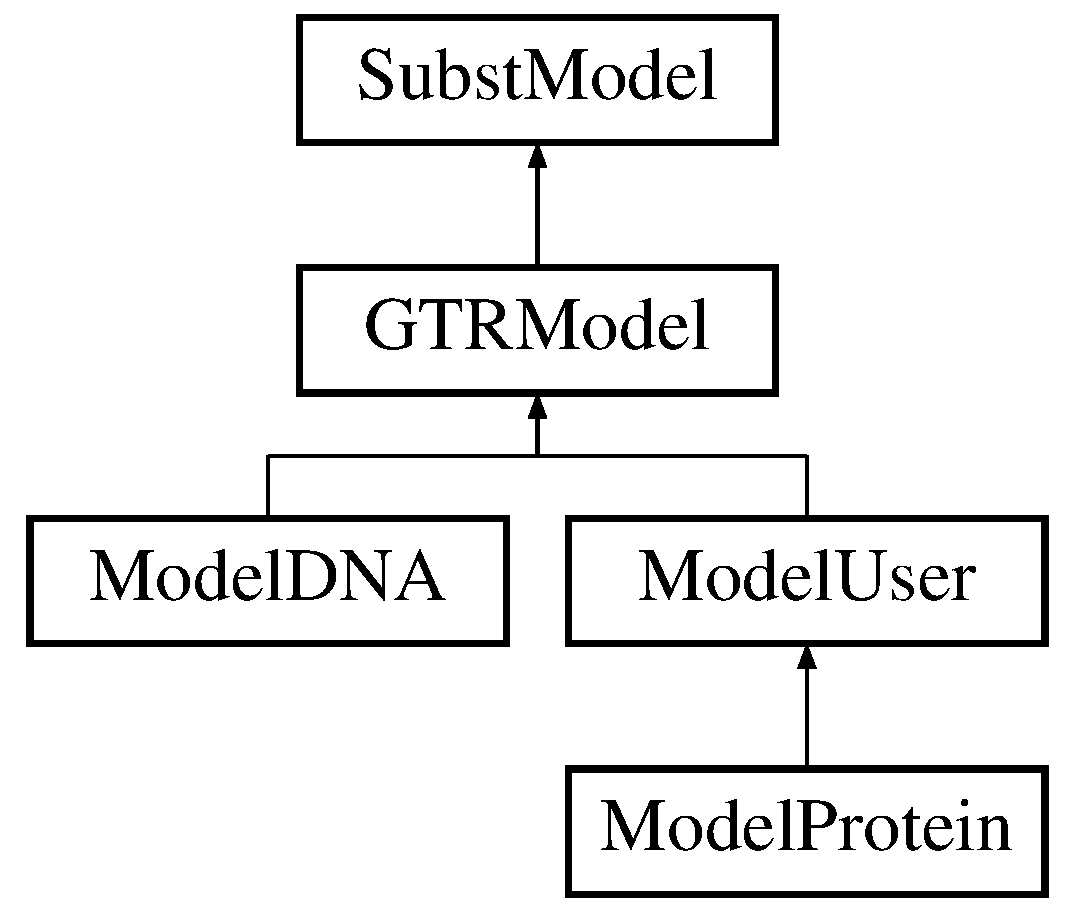
\includegraphics[height=4cm]{classSubstModel}
\end{center}
\end{figure}
\subsection*{Public Member Functions}
\begin{DoxyCompactItemize}
\item 
\hyperlink{classSubstModel_ad9629506c448db08c094f65569795242}{SubstModel} (int nstates)
\item 
virtual void \hyperlink{classSubstModel_a83997a2aaea95f2c994d88a9d1cb190e}{computeTransMatrix} (double time, double $\ast$trans\_\-matrix)
\item 
virtual void \hyperlink{classSubstModel_a18f98e25cacbd18e1b64b25d10a3e11f}{getStateFrequency} (double $\ast$state\_\-freq)
\item 
virtual double $\ast$ \hyperlink{classSubstModel_a3bea68a055833acb9dad99cb529681e5}{newTransMatrix} ()
\item 
virtual void \hyperlink{classSubstModel_ada88db5c6befc33de5ddb590667ba865}{computeTransDerv} (double time, double $\ast$trans\_\-matrix, double $\ast$trans\_\-derv1, double $\ast$trans\_\-derv2)
\item 
virtual double \hyperlink{classSubstModel_aa2d4bd724a699264b40dd5b2d129e29f}{optimizeParameters} ()
\item 
virtual void \hyperlink{classSubstModel_ac81144591a9eb6b6d9abc9e873a20af6}{writeInfo} (ostream \&out)
\item 
virtual \hyperlink{classSubstModel_accfa9c36ec87262ca1479fcdb4c95c3d}{$\sim$SubstModel} ()
\end{DoxyCompactItemize}
\subsection*{Public Attributes}
\begin{DoxyCompactItemize}
\item 
int \hyperlink{classSubstModel_abc3ccd407830f359e794ac3fd51a5559}{num\_\-states}
\item 
string \hyperlink{classSubstModel_a28fd43ca59508025c8faa9365861a3d8}{name}
\end{DoxyCompactItemize}


\subsection{Detailed Description}
Substitution model abstract class

\begin{DoxyAuthor}{Author}
BUI Quang Minh, Steffen Klaere, Arndt von Haeseler $<$\href{mailto:minh.bui@univie.ac.at}{\tt minh.bui@univie.ac.at}$>$ 
\end{DoxyAuthor}


\subsection{Constructor \& Destructor Documentation}
\hypertarget{classSubstModel_ad9629506c448db08c094f65569795242}{
\index{SubstModel@{SubstModel}!SubstModel@{SubstModel}}
\index{SubstModel@{SubstModel}!SubstModel@{SubstModel}}
\subsubsection[{SubstModel}]{\setlength{\rightskip}{0pt plus 5cm}SubstModel::SubstModel (int {\em nstates})}}
\label{classSubstModel_ad9629506c448db08c094f65569795242}
constructor 
\begin{DoxyParams}{Parameters}
\item[{\em nstates}]number of states, e.g. 4 for DNA, 20 for proteins. \end{DoxyParams}
\hypertarget{classSubstModel_accfa9c36ec87262ca1479fcdb4c95c3d}{
\index{SubstModel@{SubstModel}!$\sim$SubstModel@{$\sim$SubstModel}}
\index{$\sim$SubstModel@{$\sim$SubstModel}!SubstModel@{SubstModel}}
\subsubsection[{$\sim$SubstModel}]{\setlength{\rightskip}{0pt plus 5cm}SubstModel::$\sim$SubstModel ()\hspace{0.3cm}{\ttfamily  \mbox{[}virtual\mbox{]}}}}
\label{classSubstModel_accfa9c36ec87262ca1479fcdb4c95c3d}
destructor 

\subsection{Member Function Documentation}
\hypertarget{classSubstModel_ada88db5c6befc33de5ddb590667ba865}{
\index{SubstModel@{SubstModel}!computeTransDerv@{computeTransDerv}}
\index{computeTransDerv@{computeTransDerv}!SubstModel@{SubstModel}}
\subsubsection[{computeTransDerv}]{\setlength{\rightskip}{0pt plus 5cm}void SubstModel::computeTransDerv (double {\em time}, \/  double $\ast$ {\em trans\_\-matrix}, \/  double $\ast$ {\em trans\_\-derv1}, \/  double $\ast$ {\em trans\_\-derv2})\hspace{0.3cm}{\ttfamily  \mbox{[}virtual\mbox{]}}}}
\label{classSubstModel_ada88db5c6befc33de5ddb590667ba865}
compute the transition probability matrix.and the derivative 1 and 2 
\begin{DoxyParams}{Parameters}
\item[{\em time}]time between two events \item[{\em trans\_\-matrix}](OUT) the transition matrix between all pairs of states. Assume trans\_\-matrix has size of num\_\-states $\ast$ num\_\-states. \item[{\em trans\_\-derv1}](OUT) the 1st derivative matrix between all pairs of states. \item[{\em trans\_\-derv2}](OUT) the 2nd derivative matrix between all pairs of states. \end{DoxyParams}


Reimplemented in \hyperlink{classGTRModel_a9f6c7532d57b0e41d95dd95c5972cf5b}{GTRModel}.\hypertarget{classSubstModel_a83997a2aaea95f2c994d88a9d1cb190e}{
\index{SubstModel@{SubstModel}!computeTransMatrix@{computeTransMatrix}}
\index{computeTransMatrix@{computeTransMatrix}!SubstModel@{SubstModel}}
\subsubsection[{computeTransMatrix}]{\setlength{\rightskip}{0pt plus 5cm}void SubstModel::computeTransMatrix (double {\em time}, \/  double $\ast$ {\em trans\_\-matrix})\hspace{0.3cm}{\ttfamily  \mbox{[}virtual\mbox{]}}}}
\label{classSubstModel_a83997a2aaea95f2c994d88a9d1cb190e}
compute the transition probability matrix. One should override this function when defining new model. The default is the Juke-\/Cantor model, valid for all kind of data (DNA, AA, Codon, etc) 
\begin{DoxyParams}{Parameters}
\item[{\em time}]time between two events \item[{\em trans\_\-matrix}](OUT) the transition matrix between all pairs of states. Assume trans\_\-matrix has size of num\_\-states $\ast$ num\_\-states. \end{DoxyParams}


Reimplemented in \hyperlink{classGTRModel_aa779b66b3824c4e956db7b56dee668c2}{GTRModel}.\hypertarget{classSubstModel_a18f98e25cacbd18e1b64b25d10a3e11f}{
\index{SubstModel@{SubstModel}!getStateFrequency@{getStateFrequency}}
\index{getStateFrequency@{getStateFrequency}!SubstModel@{SubstModel}}
\subsubsection[{getStateFrequency}]{\setlength{\rightskip}{0pt plus 5cm}void SubstModel::getStateFrequency (double $\ast$ {\em state\_\-freq})\hspace{0.3cm}{\ttfamily  \mbox{[}virtual\mbox{]}}}}
\label{classSubstModel_a18f98e25cacbd18e1b64b25d10a3e11f}
compute the state frequency vector. One should override this function when defining new model. The default is equal state sequency, valid for all kind of data. 
\begin{DoxyParams}{Parameters}
\item[{\em state\_\-freq}](OUT) state frequency vector. Assume state\_\-freq has size of num\_\-states \end{DoxyParams}


Reimplemented in \hyperlink{classGTRModel_aa7cdd1fb6852faccc185284c075c918b}{GTRModel}.\hypertarget{classSubstModel_a3bea68a055833acb9dad99cb529681e5}{
\index{SubstModel@{SubstModel}!newTransMatrix@{newTransMatrix}}
\index{newTransMatrix@{newTransMatrix}!SubstModel@{SubstModel}}
\subsubsection[{newTransMatrix}]{\setlength{\rightskip}{0pt plus 5cm}double $\ast$ SubstModel::newTransMatrix ()\hspace{0.3cm}{\ttfamily  \mbox{[}virtual\mbox{]}}}}
\label{classSubstModel_a3bea68a055833acb9dad99cb529681e5}
allocate memory for a transition matrix. One should override this function when defining new model such as Gamma model. The default is to allocate a double vector of size num\_\-states $\ast$ num\_\-states. This is equivalent to the memory needed by a square matrix. \begin{DoxyReturn}{Returns}
the pointer to the newly allocated transition matrix 
\end{DoxyReturn}
\hypertarget{classSubstModel_aa2d4bd724a699264b40dd5b2d129e29f}{
\index{SubstModel@{SubstModel}!optimizeParameters@{optimizeParameters}}
\index{optimizeParameters@{optimizeParameters}!SubstModel@{SubstModel}}
\subsubsection[{optimizeParameters}]{\setlength{\rightskip}{0pt plus 5cm}virtual double SubstModel::optimizeParameters ()\hspace{0.3cm}{\ttfamily  \mbox{[}inline, virtual\mbox{]}}}}
\label{classSubstModel_aa2d4bd724a699264b40dd5b2d129e29f}
optimize model parameters. One should override this function when defining new model. The default does nothing since it is a Juke-\/Cantor type model, hence no parameters involved. \begin{DoxyReturn}{Returns}
the best likelihood 
\end{DoxyReturn}


Reimplemented in \hyperlink{classGTRModel_a01c47ec7ac4b856e60aa3e4339e0044a}{GTRModel}.\hypertarget{classSubstModel_ac81144591a9eb6b6d9abc9e873a20af6}{
\index{SubstModel@{SubstModel}!writeInfo@{writeInfo}}
\index{writeInfo@{writeInfo}!SubstModel@{SubstModel}}
\subsubsection[{writeInfo}]{\setlength{\rightskip}{0pt plus 5cm}virtual void SubstModel::writeInfo (ostream \& {\em out})\hspace{0.3cm}{\ttfamily  \mbox{[}inline, virtual\mbox{]}}}}
\label{classSubstModel_ac81144591a9eb6b6d9abc9e873a20af6}
write information 
\begin{DoxyParams}{Parameters}
\item[{\em out}]output stream \end{DoxyParams}


Reimplemented in \hyperlink{classGTRModel_a233f9b473e4e3c549d801ff8a084e35e}{GTRModel}.

\subsection{Member Data Documentation}
\hypertarget{classSubstModel_a28fd43ca59508025c8faa9365861a3d8}{
\index{SubstModel@{SubstModel}!name@{name}}
\index{name@{name}!SubstModel@{SubstModel}}
\subsubsection[{name}]{\setlength{\rightskip}{0pt plus 5cm}string {\bf SubstModel::name}}}
\label{classSubstModel_a28fd43ca59508025c8faa9365861a3d8}
name of the model \hypertarget{classSubstModel_abc3ccd407830f359e794ac3fd51a5559}{
\index{SubstModel@{SubstModel}!num\_\-states@{num\_\-states}}
\index{num\_\-states@{num\_\-states}!SubstModel@{SubstModel}}
\subsubsection[{num\_\-states}]{\setlength{\rightskip}{0pt plus 5cm}int {\bf SubstModel::num\_\-states}}}
\label{classSubstModel_abc3ccd407830f359e794ac3fd51a5559}
number of states 

The documentation for this class was generated from the following files:\begin{DoxyCompactItemize}
\item 
src/substmodel.h\item 
src/substmodel.cpp\end{DoxyCompactItemize}

\hypertarget{structTaxaSetName}{
\section{TaxaSetName Struct Reference}
\label{structTaxaSetName}\index{TaxaSetName@{TaxaSetName}}
}


{\ttfamily \#include $<$msetsblock.h$>$}\subsection*{Public Attributes}
\begin{DoxyCompactItemize}
\item 
\hyperlink{classNxsString}{NxsString} \hyperlink{structTaxaSetName_a9adc1c9de597527395035d3cc40b7142}{name}
\item 
vector$<$ \hyperlink{classNxsString}{NxsString} $>$ \hyperlink{structTaxaSetName_a4471e5498ef139c69206baed2675c84d}{taxlist}
\end{DoxyCompactItemize}


\subsection{Detailed Description}
a taxa set with name 

\subsection{Member Data Documentation}
\hypertarget{structTaxaSetName_a9adc1c9de597527395035d3cc40b7142}{
\index{TaxaSetName@{TaxaSetName}!name@{name}}
\index{name@{name}!TaxaSetName@{TaxaSetName}}
\subsubsection[{name}]{\setlength{\rightskip}{0pt plus 5cm}{\bf NxsString} {\bf TaxaSetName::name}}}
\label{structTaxaSetName_a9adc1c9de597527395035d3cc40b7142}
set name \hypertarget{structTaxaSetName_a4471e5498ef139c69206baed2675c84d}{
\index{TaxaSetName@{TaxaSetName}!taxlist@{taxlist}}
\index{taxlist@{taxlist}!TaxaSetName@{TaxaSetName}}
\subsubsection[{taxlist}]{\setlength{\rightskip}{0pt plus 5cm}vector$<${\bf NxsString}$>$ {\bf TaxaSetName::taxlist}}}
\label{structTaxaSetName_a4471e5498ef139c69206baed2675c84d}
string vector of taxa names 

The documentation for this struct was generated from the following file:\begin{DoxyCompactItemize}
\item 
src/msetsblock.h\end{DoxyCompactItemize}

\printindex
\end{document}
